% =================================================================================
% Hier ausw�hlen, ob TUD-Design oder nicht
% =================================================================================
\newif\ifTUDdesign
\TUDdesigntrue					% TUD-Design
%\TUDdesignfalse				% F�r Rechner ohne installierte TUDdesign-Pakete
% =================================================================================


% =================================================================================
% Hier Daten f�r studentische Arbeit eingeben
% =================================================================================
\newcommand{\SADATyp}{Projektseminar}
\newcommand{\SADATitel}{Aufbau und Regelung eines Ballbots}
\newcommand{\SADAStadt}{Darmstadt}
\newcommand{\SADAAutor}{Florian M�ller \newline Markus Lamprecht \newline Michael Suffel}
\newcommand{\SADABetreuer}{Dr.-Ing. Eric Lenz}
\newcommand{\SADABetreuerII}{}
\newcommand{\SADABetreuerIII}{}
\newcommand{\SADABegin}{16. Oktober 2017}
\newcommand{\SADAAbgabe}{16. Februar 2018}
\newcommand{\SADASeminar}{09. April 2018} %Pr�si
% =================================================================================


% =================================================================================
% Auswahl des IAT-Fachgebiets (rtm / rtp)
% =================================================================================
\newif\ifrtm
\rtmtrue	% rtm
%\rtmfalse	% rtp
% =================================================================================


% =================================================================================
% Erkl�rung, dass die Arbeit ohne Hilfe Dritter etc. erstellt wurde
% =================================================================================
\def\SADAVarianteErklaerung{ETIT}		% FB 18, Elektrotechnik
%\def\SADAVarianteErklaerung{MBDA}		% FB 16, Maschinenbau, Diplomarbeit
%\def\SADAVarianteErklaerung{MBSA}		% FB 16, Maschinenbau, Studienarbeit
% =================================================================================


% =================================================================================
% Ausnahmen von der automatischen Silbentrennung
% =================================================================================
\hyphenation{Aktu-ali-sie-rung Screen-shots Pa-rallel-ro-bo-ter Zu-stands-raum-mo-del-le nach-voll-zieh-bar Pro-jekt-se-mi-nar}
% =================================================================================


% =================================================================================
% Hier NIICHTS �ndern!
% =================================================================================
\ifTUDdesign
	\documentclass[11pt, twoside, colorback, accentcolor=tud2c, nopartpage, bigchapter, fleqn, ngerman, longdoc]{tudreport}
\else
	\documentclass[11pt, a4paper, twoside, fleqn, ngerman]{scrreprt}
  % F�r Entwurf auf Rechnern ohne installierte TUDdesign-Pakete	
	\usepackage{exscale}	% Korrektur math-Zeichen
	\usepackage{eurosym}
\fi
% Dieses File dient zum einbinden wichtiger und n�tzlicher Pakete.
% Nicht alle Pakete m�ssen verwendet werden.
%
\usepackage{t1enc}			% evtl. dc-Fonts
\usepackage[T1]{fontenc}	% F�r Silbentrennung bei W�rten mit Sonderzeichen (z.B. Umlaute)
\usepackage[latin1]{inputenc}
							% Um Sonderzeichen (�, �, �, ...) direkt eingeben zu k�nnen
\usepackage[english,ngerman]{babel}
							% F�r Sprachenspezifisches
							% ngerman ist schon als globale Option definiert

\usepackage{helvet}			% Helvetica als Standard-Sans-Schriftart
\usepackage[stable]{footmisc}
\usepackage{booktabs}


\usepackage{graphicx}		% zum Einbinden von Postscript
\usepackage{psfrag}			% Beschriftung der Bilder
\usepackage{amsmath}		% Mehr mathematischen Formelsatz
%\usepackage{amssymb}		% Mehr mathematische Symbole
%\usepackage{amsthm}

\usepackage{float}			% F�r Parameter [H] bei Flie�objekten

\usepackage{epsfig}			% Um eps-Bilder einzubinden
\usepackage{scrhack}    % Um Warnung "float@addtolists detected" zu unterdr�cken 
\usepackage{subfig}			% F�r Unterabbildungen
\usepackage{ltxtable} 		% Vereinigt TabularX und Longtable
\usepackage{longtable}
\usepackage{rotating}		% Zum Drehen von Objekten
\usepackage{bibgerm}		% F�r deutsche Literaturverwaltung
%\usepackage{wrapfig}		% F�r kleine Bilder am Rand
%\usepackage{floatflt}		% Alternative zu wrapfig
%\usepackage[hang]{caption}	% Damit mehrzeilige Bildunterschriften gut aussehen
\usepackage{upgreek}		% F�r nicht-kursive kleine griechischen Buchstaben

\usepackage{multirow}		% F�r mehrzeilige Felder in Tabellen

\usepackage{textcomp}		% F�r Sonderzeichen im normalen Text
							% (offensichtlich in tudreport schon eingebunden)
\usepackage[ngerman]{varioref}		% F�r vref
\usepackage{color}			% F�r farbigen Text
\usepackage{placeins}		% F�r \FloatBarrier
\usepackage{xspace}
\usepackage{icomma}			% Damit nach Dezimalkommas kein Abstand eingef�gt wird
							% (in math-Umgebungen)

\usepackage{cancel}			% Zum Wegstreichen von Gleichungstermen

\usepackage{array}			% F�r Zellentyp "m{}" in tabular-Umgebungen (Vertikal zentriert)

\usepackage{listings}		% Um formatierten Quellcode einzubinden
\usepackage{moreverb}		% F�r Umgebung "`verbatimtab"' (Verbatim mit Tabs)
\renewcommand{\verbatimtabsize}{4\relax}	% Standardtabweite in "`verbatimtab"'

											% ist 4 Zeichen


% Das Packet hyperref immer als letztes einbinden (nur bookmark darf danach kommen)!
%\usepackage[ps2pdf, colorlinks=false, pdfborder={0 0 0}]{hyperref}
%\usepackage[ps2pdf]{hyperref}	% F�r Verlinkungen im erzeugten pdf
\usepackage{hyperref}	% F�r Verlinkungen im erzeugten pdf
\usepackage{bookmark}
\usepackage{url}

% Markus includes:
\usepackage{array}
\newcolumntype{L}[1]{>{\raggedright\let\newline\\\arraybackslash\hspace{0pt}}m{#1}}
\newcolumntype{C}[1]{>{\centering\let\newline\\\arraybackslash\hspace{0pt}}m{#1}}
\newcolumntype{R}[1]{>{\raggedleft\let\newline\\\arraybackslash\hspace{0pt}}m{#1}}
\usepackage{footnote}
\makesavenoteenv{tabular} % footnotes in tabular env.

% Florian includes:
\usepackage{tikz}
%\usepackage{etoolbox}
%\makeatletter
%\AtBeginDocument{
%\patchcmd{\use@@tikzlibrary}{\global}{}{}{}
%}
%\makeatother
\usepackage{pgfplots} 
\usepackage{pgfgantt}
\usepackage{pdflscape}
\pgfplotsset{compat=newest} 
\pgfplotsset{plot coordinates/math parser=false}
\newlength\figH
\newlength\figW
\setlength{\figH}{7cm}
\setlength{\figW}{14cm}				% verwendete Pakete einbinden
% =================================================================================
% Definitionen f�r rtm / rtp
% =================================================================================
\ifrtm
	\newcommand{\SADAProf}{Prof. Dr.-Ing. Ulrich Konigorski}
  \newcommand{\SADAinstitut}{Institut f�r Automatisierungstechnik und Mechatronik\\
                             Fachgebiet Regelungstechnik und Mechatronik\\
                             \SADAProf}
  \newcommand{\SADAwebsite}{www.rtm.tu-darmstadt.de}
  \newcommand{\SADAtel}{06151/16-4167}
  \newcommand{\SADAlogo}{
\includegraphics[width=3cm]{./common/IAT_rtm}}
\else
  \newcommand{\SADAProf}{Prof. Dr.-Ing. Dr. h.c. Rolf Isermann}
  \newcommand{\SADAinstitut}{Institut f�r Automatisierungstechnik\\
                             und Mechatronik\\
                             FG Regelungstechnik und Prozessautomatisierung\\
                             \SADAProf}
  \newcommand{\SADAwebsite}{http://www.rtm.tu-darmstadt.de/rtp.html}
  \newcommand{\SADAtel}{06151/16-5465}
  \newcommand{\SADAlogo}{
\includegraphics[width=3cm]{./common/rtplogo}}
\fi
%\institution{\SADAinstitut}
% =================================================================================		
		
		
% =================================================================================
% Definitionen f�r die Erkl�rung, dass die Arbeit ohne Hilfe Dritter etc. erstellt wurde
% =================================================================================
% Die folgende Zeile deklariert die m�glichen Varianten der Erkl�rung, dass die
% Arbeit ohne Hilfe Dritter etc. erstellt wurde.
\def\ETIT{ETIT}\def\MBSA{MBSA}\def\MBDA{MBDA}
% =================================================================================


% =================================================================================
% Definitionen aus tudreport-Vorlage
% =================================================================================
\newif\ifTUDmargin
%\TUDmargintrue		% Sehr breiter rechter Rand
\TUDmarginfalse		% Schmaler (normaler) rechter Rand

\ifTUDmargin	% ggf. breiten Rand setzen
  \geometry{marginparsep=4.2mm,marginparwidth=28.64mm}
\fi

\newlength{\longtablewidth}
\setlength{\longtablewidth}{0.7\linewidth}
\addtolength{\longtablewidth}{-\marginparsep}
\addtolength{\longtablewidth}{-\marginparwidth}
% =================================================================================


% =================================================================================
% Farbige Deckseite, graue Balken auf allen anderen Seiten
% =================================================================================
\newif\ifOnlyColorFront
\OnlyColorFronttrue	    % Balken nur auf Deckblatt farbig
% \OnlyColorFrontfalse		% alle Balken farbig
% =================================================================================


% =================================================================================
% Befehle, die in scrreprt nicht exisiteren werden hier definiert, wenn diese
% Klasse verwendet wird.
% Auch die Seitenr�nder werden angepasst, so dass es grob wie mit tudreport
% aussieht.
% =================================================================================
\ifTUDdesign
	\title{\SADATitel}
	\subtitle{\SADAAutor}
	\subsubtitle{\SADATyp\ -- \SADAAbgabe  \\Betreuer: \SADABetreuer{} \SADABetreuerII{} \SADABetreuerIII{}}
	\setinstitutionlogo[height]{common/rtm_mit_schrift}
	\geometry{left=30mm, right=20mm, top=15mm, bottom=20mm}
\else
	\title{\SADATitel}
	\subtitle{}
	\author{\SADAAutor}	% scrreprt erwartet Autor
	
	\newcommand{\subsubtitle}[1]{}
	\newcommand{\settitlepicture}[1]{}
	\newcommand{\printpicturesize}{}
	\newcommand{\institution}[1]{}
    \pagestyle{headings}

  % Diese Pakete nur extra einbinden, wenn NICHT tudreport als Basis.
	\usepackage{amssymb}
	\usepackage{geometry}
	
% \settitlepicture{}	% Bild f�r Deckblatt
% \printpicturesize
\fi
% =================================================================================


% =================================================================================
% Anpassung Absatzformat
% =================================================================================
% Der Abstand der Zeilen betr�gt das 1,25-fache des Standard-Abstands von
% LaTeX. Da technische Arbeiten viele Formeln und Bilder enthalten, werden
% Abs�tze durch einen zus�tzlichen vertikalen Zwischenraum statt durch einen
% Einzug getrennt.
\linespread{1.25}
\setlength{\parindent}{0mm}
\setlength{\parskip}{1ex}
% =================================================================================


% =================================================================================
% Texte f�r die R�ckseite des Titelblatts vorgeben
% =================================================================================
\uppertitleback{}
\lowertitleback{}
\dedication{}
% =================================================================================


% =================================================================================
% Informationen (Meta-Daten) f�r pdf
% =================================================================================
\hypersetup{
	pdftitle = {\SADATitel},
	pdfsubject = {},
	pdfauthor = {\SADAAutor},
	pdfkeywords = {},
	pdfcreator = {},
	pdfproducer = {LaTeX with hyperref},
	pdfstartview = {Fit},
	pdfpagelayout = {SinglePage}
}
% =================================================================================
					% LaTeX-Einstellungen
% Dieses File dient zum definieren n�tzlicher Befehle.
% Es soll lediglich als Beispiel dienen, wie Befehle definiert werden, und welche Befehle n�tzlich sein k�nnen
%


% Inhalt
% ======
%	Allgemeine Abk�rzungen
%	Makros f�r Referenzen (Abbildungen, Zitate, ...)
%	Makros f�r Abbildungen
%	Makros f�r Einheiten, Exponenten
%	Makros f�r Formeln
%	Makros f�r Entwurf
%   Definitionen f�r Umgebungen



% Allgemeine Abk�rzungen
% ======================
	\newcommand{\bzw}{bzw.\@\xspace}
	\newcommand{\Bzw}{Bzw.\@\xspace}
	\newcommand{\bzgl}{bzgl.\@\xspace}
	\newcommand{\ca}{ca.\@\xspace}
	\newcommand{\evtl}{evtl.\@\xspace}
	\newcommand{\usw}{usw.\@\xspace}
	\newcommand{\etc}{etc.\@\xspace}
	\newcommand{\vgl}{vgl.\@\xspace}
	\newcommand{\Vgl}{Vgl.\@\xspace}
	\newcommand{\bspw}{bspw.\@\xspace}
	\newcommand{\Bspw}{Bspw.\@\xspace}
	\newcommand{\ggf}{ggf.\@\xspace}
	\newcommand{\Ggf}{Ggf.\@\xspace}



	\newcommand{\dah}{d.\thinspace{}h.\@\xspace}
	\newcommand{\Dah}{D.\thinspace{}h.\@\xspace}
	\newcommand{\iA}{i.\thinspace{}A.\@\xspace}
	\newcommand{\IA}{i.\thinspace{}A.\@\xspace}
	\newcommand{\ua}{u.\thinspace{}a.\@\xspace}
	\newcommand{\Ua}{U.\thinspace{}a.\@\xspace}
	\newcommand{\uU}{u.\thinspace{}U.\@\xspace}
	\newcommand{\UU}{u.\thinspace{}U.\@\xspace}
	\newcommand{\zB}{z.\thinspace{}B.\@\xspace}
	\newcommand{\ZB}{Zum Beispiel\xspace}
	\newcommand{\zT}{z.\thinspace{}T.\@\xspace}
	\newcommand{\ZT}{Z.\thinspace{}T.\@\xspace}



% Makros f�r Referenzen (Abbildungen, Zitate, ...)
% ================================================

	% Referenzierung auf Abbildungen, Tabellen, etc. (Hyperref-f�hig)
	\newcommand{\figref}[1]{\hyperref[#1]{\figurename\ \ref*{#1}}}
	\newcommand{\tabref}[1]{\hyperref[#1]{\tablename\ \ref*{#1}}}
	\newcommand{\equref}[1]{\hyperref[#1]{Gl.~(\ref*{#1})}}
	\newcommand{\defref}[1]{\hyperref[#1]{Definition~\ref*{#1}}}
	\newcommand{\figvref}[1]{\hyperref[#1]{\figurename}\vref{#1}}
	\newcommand{\tabvref}[1]{\hyperref[#1]{\tablename}\vref{#1}}
	\newcommand{\equvref}[1]{\hyperref[#1]{Gl.~(\ref*{#1}) auf Seite \pageref*{#1}}}
	\newcommand{\pagerefh}[1]{\hyperref[#1]{Seite~\pageref*{#1}}}
	\newcommand{\secref}[1]{\hyperref[#1]{Abschnitt~\ref*{#1}}}
	\newcommand{\charef}[1]{\hyperref[#1]{Kapitel~\ref*{#1}}}
	\newcommand{\lstref}[1]{\hyperref[#1]{Listing~\ref*{#1}}}


	% Zitate mit Seitenangabe in Fu�note
%	\newcommand{\citep}[2]{\cite{#1}\footnote{Seite #2}}
%	\newcommand{\citepp}[2]{\cite{#1}\footnote{Seiten #2}}
	\newcommand{\citep}[2]{\cite{#1} (S. #2)}
	\newcommand{\citepp}[2]{\cite{#1} (S. #2)}
	
	
% Makros f�r Abbildungen
% ======================
	% zum Skalieren nach Ersetzen durch psfrag
	\newcommand{\incgraphicsw}[2]{\resizebox{#1}{!}{\includegraphics{#2}}}


% Textbausteine
% =============
	% Produktnamen
	\newcommand{\Matlab}{\textsc{Matlab}}
	\newcommand{\Matlabreg}{\textsc{Matlab}\textsuperscript{\tiny \textregistered}}
	\newcommand{\MatSim}{\textsc{Matlab/Simulink}}
	\newcommand{\Simulink}{\textsc{Simulink}}
	\newcommand{\Simulinkreg}{\textsc{Simulink}\textsuperscript{\tiny \textregistered}}



% Makros f�r Einheiten, Exponenten
% ================================

	\newcommand{\unit}[1] { \ensuremath{\mathrm{#1}}}
	
	% Wert mit Einheit (mit kleinem Leerzeichen dazwischen), aus Text- UND Math-Modus
	\newcommand{\valunit}[2]{\ensuremath{#1\,\mrm{#2}}}


	% "�C", im Text- oder Mathe-Modus
	\newcommand{\degC}{
		\ifmmode
			^\circ \mrm{C}%
		\else
			\textdegree C%
		\fi}

	\newcommand{\degree}{
		\ifmmode
			^\circ%
		\else
			\textdegree%
		\fi}
	
	% F�r Exponentenschreibweise ( Anwendung: 123\E{3} )
	\newcommand{\E}[1]{ \ensuremath{\cdot 10^{#1}} }
	
	\newcommand{\eexp}[1]{ \mathrm{e}^{#1} }
	\newcommand{\iu}{ \mathrm{j} }

	\newcommand{\todots}{ ,\,\hdots,\, }


% Makros f�r Formeln
% ==================

    \newcommand{\mat}[1]{{\ensuremath{\boldsymbol{\mathrm{#1}}}}}

	\newcommand{\AP} { \mathrm{AP} }
	\newcommand{\doti} {(i)^\cdot}

	% Definition f�r Vektor und Matizen
	\newcommand{\ve}[1]{\ensuremath{\mathbf{#1}}}
	\newcommand{\ma}[1]{\ensuremath{\mathbf{#1}}}

	% Definition f�r Vektor und Matizen
	\newcommand{\ves}[1]{\ensuremath{\boldsymbol{#1}}}
	\newcommand{\mas}[1]{\ensuremath{\boldsymbol{#1}}}
	
	
	\newcommand{\inprod}[2]{\langle #1,\,#2 \rangle}
	
	\newcommand{\ul}[1]{\underline{#1}}

	% gerades "d" (z.B. f�r Integral)
	\newcommand{\ud} { \mathrm{d} }
	
	% normaler Text in Formeln
	\newcommand{\tn}[1] { \textnormal{#1} }
	
	% nicht-kursive Schrift in Formeln
	\newcommand{\mrm}[1] { \mathrm{#1}}
	
	% gerades "T" f�r Transponiert
	\newcommand{\transp}{\mathrm{T}}
	
	% gerades "rg"
	\newcommand{\rang}[1]{\mathrm{rg}(#1)}

	% F�r geklammerte Ausdr�cke mit Index (Subscript)
	% (einmal mit kursiven Index, einmal mit geradem Index)
	\newcommand{\grpsb}[2] { \left( #1 \right)_{#2} }
	\newcommand{\grprsb}[2] { \left( #1 \right)_{\mathrm{#2}} }

	% Ableitungen und Integrale
		% "normale" Ableitung (mit geraden "d"s)
		\newcommand{\normd}[2] { \frac{\mathrm{d} #1 }{\mathrm{d} #2 } }
		\newcommand{\normdat}[3] { \left. \frac{\mathrm{d} #1 }{\mathrm{d} #2 } \right|_{#3} }
	
		% Materielle Ableitung
		\newcommand{\matd}[2] { \frac{\mathrm{D} #1 }{\mathrm{D} #2 } }
		\newcommand{\matdat}[3] { \left. \frac{\mathrm{D} #1 }{\mathrm{D} #2 } \right|_{#3} }
	
		% Partielle Ableitung
		\newcommand{\partiald}[2] { \frac{\partial #1 }{\partial #2 } }
		\newcommand{\partialdat}[3] { \left. \frac{\partial #1 }{\partial #2 } \right|_{#3} }
	
	
	% Transformationen
	\newcommand{\FT}[1] { \mathfrak{F} \left\{ #1 \right\} }
	\newcommand{\FTabs}[1]{\left| \mathfrak{F} \left\{ #1 \right\} \right|}
	\newcommand{\IFT}[1] { \mathfrak{F}^{-1} \left\{ #1 \right\} }
	\newcommand{\DFT}[1]{\mathrm{DFT} \left\{ #1 \right\}}
	\newcommand{\DFTabs}[1]{\left| \mathrm{DFT} \left\{ #1 \right\} \right|}

	\newcommand{\Laplace}[1]{\mathfrak{L}\left (#1\right)} % L-Transformation
	\newcommand{\InvLaplace}[1]{\mathfrak{L^{-1}}\left (#1\right )} % L-Transformation, invers
	\newcommand{\invtrans}{\quad\bullet\!\!-\!\!\!-\!\!\circ\quad}
	\newcommand{\trans}{\quad\circ\!\!-\!\!\!-\!\!\bullet\quad}


	\newcommand{\mlfct}[1]{{\tt #1}}
	\newcommand{\mlvar}[1]{{\tt #1}}


	% Manche textcomp-Zeichen funktionieren mit dem TU-Design nicht, diese k�nnen dann mit diesem
	% Befehl gesetzt werden.
	\newcommand{\textcompstdfont}[1]{{\fontfamily{cmr} \fontseries{m} \fontshape{n} \selectfont #1}}
	


% =================================================================================
% Defintionen f�r Mathe-Umgebungen
% =================================================================================
	
\newtheorem{theorem}{Satz}
\newtheorem{lemma}[theorem]{Lemma}	% Selber Z�hler wie theorem
\newtheorem{definition}{Definition}
% =================================================================================


% =================================================================================
% Defintionen f�r Beispiel-Umgebung
% =================================================================================
\newcounter{examplenumber}[chapter]      % Neuer Counter bspnummer nummeriert nach Kapitel
\def\theexamplenumber{\thechapter.\arabic{examplenumber}}

\newenvironment{example}[1][]
{\vskip 3\parskip plus 1pt minus 1pt \refstepcounter{examplenumber}
\vspace{.3cm} \begin{addmargin}[1cm]{0cm} \noindent \textbf{Beispiel \theexamplenumber}: \textbf{#1}\par}
{\end{addmargin} \par \vspace{.3cm}}

% Alternative, einfachere Beispielumgebung:
% \newtheorem{example}{Beispiel}
% =================================================================================




% =================================================================================
% Definitionen f�r Listingsumgebung
% =================================================================================

\lstloadlanguages{Matlab}

\lstdefinestyle{Matlab_colored_smallfont}
{
	language = Matlab,
	tabsize = 4,
	framesep = 3mm,
	frame=tb,
	classoffset = 0,	
	basicstyle = \footnotesize\ttfamily,
	keywordstyle = \bfseries\color[rgb]{0,0,1},
	commentstyle = \itshape\color[rgb]{0.133,0.545,0.133},
	stringstyle = \color[rgb]{0.627,0.126,0.941},
	extendedchars = true,
	breaklines = true,
	prebreak = \textrightarrow,
	postbreak = \textleftarrow,
	%escapeinside = {(*@}{@*)},
	%moredelim = [s][\itshape\color[rgb]{0.5,0.5,0.5}]{[.}{.]},
	numbers = left,
	numberstyle = \tiny,
	stepnumber = 5
}

\lstdefinestyle{Matlab_colored}
{
	language = Matlab,
	tabsize = 4,
	framesep = 3mm,
	frame=tb,
	classoffset = 0,	
	basicstyle = \ttfamily,
	keywordstyle = \bfseries\color[rgb]{0,0,1},
	commentstyle = \itshape\color[rgb]{0.133,0.545,0.133},
	stringstyle = \color[rgb]{0.627,0.126,0.941},
	extendedchars = true,
	breaklines = true,
	prebreak = \textrightarrow,
	postbreak = \textleftarrow,
	%escapeinside = {(*@}{@*)},
	%moredelim = [s][\itshape\color[rgb]{0.5,0.5,0.5}]{[.}{.]},
	numbers = left,
	numberstyle = \tiny,
	stepnumber = 5
}


\lstdefinestyle{C_colored_smallfont}
{
	language=C,
	tabsize = 4,
	framesep = 3mm,
	frame=tb,	
	classoffset = 0,	
	basicstyle = \footnotesize\ttfamily,
	keywordstyle = \bfseries\color[rgb]{0,0,1},
	commentstyle = \itshape\color[rgb]{0.133,0.545,0.133},
	stringstyle = \color[rgb]{0.627,0.126,0.941},
	extendedchars = true,
	breaklines = true,
	prebreak = \textrightarrow,
	postbreak = \textleftarrow,
	%escapeinside = {(*@}{@*)},
	%moredelim = [s][\itshape\color[rgb]{0.5,0.5,0.5}]{[.}{.]},
	numbers = left,
	numberstyle = \tiny,
	stepnumber = 5
}

\lstdefinestyle{C_colored}
{
	language=C,
	tabsize = 4,
	framesep = 3mm,
	frame=tb,
	classoffset = 0,	
	basicstyle = \ttfamily,
	keywordstyle = \bfseries\color[rgb]{0,0,1},
	commentstyle = \itshape\color[rgb]{0.133,0.545,0.133},
	stringstyle = \color[rgb]{0.627,0.126,0.941},
	extendedchars = true,
	breaklines = true,
	prebreak = \textrightarrow,
	postbreak = \textleftarrow,
	%escapeinside = {(*@}{@*)},
	%moredelim = [s][\itshape\color[rgb]{0.5,0.5,0.5}]{[.}{.]},
	numbers = left,
	numberstyle = \tiny,
	stepnumber = 5
}
		% oft verwendete Befehle
\settitlepicture{Bilder/Markus/title_pic.png}
% =================================================================================


% =================================================================================
% Hier beginnt das eigentliche Dokument
% =================================================================================
\begin{document}

\selectlanguage{ngerman}
\maketitle

% Die Farbe der Identit�tsleiste wird auf Grau umgestellt, damit nicht alle Seiten
% farbig gedruckt werden m�ssen
\ifTUDdesign
	\ifOnlyColorFront	% ggf. nachfolgende Balken andere Farbe zuweisen
		\makeatletter 	% ben�tigt, um die @-Befehle auszuf�hren
    \renewcommand{\@TUD@largerulecolor}{\color{tud0b}}% am besten gleiche Farbe wie in der ersten Zeile und die Zahl durch die 0 ersetzen, dann hat das Grau die richtige Intensit�t
    \makeatother
	\fi
\fi


\pagenumbering{roman}	% Bis zum Hauptteil werden r�mische Seitenzahlen verwendet

% =================================================================================
% Spezielle Seiten f�r studentische Arbeiten
% =================================================================================
\cleardoublepage
\section*{Aufgabenstellung}
F�r schriftliche Arbeiten (Pro-/Projektseminar, Studien-, Bachelor-, Master-, Diplomarbeiten, \etc) soll Studierenden ein \LaTeX-Dokument zur Verf�gung gestellt werden, das die Vorgaben aus den \emph{Richtlinien zur Anfertigung von Studien- und Diplomarbeiten}~\cite{Richtlinien} umsetzt. Die Dokumentation soll die Funktionen des Dokumentes beschreiben und Hinweise zu ihrer Anwendung geben.

Grundlage ist die \verb|tudreport|-Klasse. Die damit erstellten Arbeiten m�ssen sowohl zum Ausdrucken geeignet sein als auch f�r die Bildschirmdarstellung und die elektronische Archivierung als PDF-Datei.

\vspace{0.5cm}
\begin{tabular}{ll}
Beginn: & \SADABegin \\
Ende:   & \SADAAbgabe \\
Seminar:& \SADASeminar
\end{tabular}

\vspace{1cm}

\begin{tabular}{ll}
\rule{7cm}{0.4pt} \hspace{1cm} & \rule{7cm}{0.4pt} \\
\SADAProf & \SADABetreuer\\
 &\SADABetreuerII\\
 &\SADABetreuerIII
\end{tabular}

\vfill
{\renewcommand{\baselinestretch}{1} % f�r diesen Abschnitt einfacher Zeilenabstand
\normalsize % anwenden des Zeilenabstandes
\begin{minipage}{0.8\textwidth}
	Technische Universit�t Darmstadt\\
	\SADAinstitut\\[0.5cm]
%
	Landgraf-Georg-Stra�e 4\\
	64283 Darmstadt\\
	Telefon \SADAtel\\
	\SADAwebsite
\end{minipage}
\begin{minipage}{0.2\textwidth}
\flushright  % rechtsb�ndig
\ \\[2.7cm]
\SADAlogo\;
\end{minipage}}



\cleardoublepage
\ \\[3cm]	% Diese Zeile erzeugt einen Abstand von 4cm zur ersten Zeile, die nur ein Leerzeichen
			% enth�lt

\ifx\SADAVarianteErklaerung\ETIT
	\section*{Erkl�rung}
	\noindent
	Hiermit versichere ich, dass ich die vorliegende Arbeit ohne Hilfe Dritter und nur mit den angegebenen Quellen und Hilfsmitteln angefertigt habe. Alle Stellen, die aus den Quellen entnommen wurden, sind als solche kenntlich gemacht. Diese Arbeit hat in gleicher oder �hnlicher Form noch keiner Pr�fungsbeh�rde vorgelegen.\vspace*{20mm} \\
	\noindent
	\begin{tabular}{ll}
		\SADAStadt, den \SADAAbgabe	\hspace{1cm}	& \rule{0.4\textwidth}{0.4pt}\\
		& Florian M�ller\\ & \\ &\rule{0.4\textwidth}{0.4pt} \\ & Markus Lamprecht\\ & \\ & \rule{0.4\textwidth}{0.4pt} \\ & Michael Suffel
	\end{tabular}
	


\else\ifx\SADAVarianteErklaerung\MBDA
	\section*{Erkl�rungen}
	\noindent
	Hiermit erkl�re ich an Eides statt, dass ich die vorliegende \SADATyp\ mit dem Titel\ \glqq\SADATitel\grqq\ selb\-st�ndig und ohne fremde Hilfe verfasst, andere als die angegebenen Quellen und Hilfsmittel nicht benutzt und die aus anderen	Quellen entnommenen Stellen als solche gekennzeichnet habe.\\
	Diese Arbeit hat in gleicher oder �hnlicher Form noch keiner Pr�fungsbeh�rde vorgelegen.\vspace*{20mm} \\
	\noindent
	\begin{tabular}{ll}
		\SADAStadt, den \SADAAbgabe	\hspace{1cm}	& \rule{0.4\textwidth}{0.4pt}\\
										& \SADAAutor
	\end{tabular}
	
	
	\vspace{40mm}
	\noindent
	Ich bin damit einverstanden, dass die TU Darmstadt das Urheberrecht an meiner \SADATyp\ zu wissenschaftlichen Zwecken nutzen kann.\vspace*{20mm} \\
	\noindent
	\begin{tabular}{ll}
		\SADAStadt, den \SADAAbgabe	\hspace{1cm}	& \rule{0.4\textwidth}{0.4pt}\\
										& \SADAAutor
	\end{tabular}

	{\huge Hier fehlt noch was!}
	
	
\else\ifx\SADAVarianteErklaerung\MBSA
	\section*{Erkl�rungen}
	\noindent
	Hiermit erkl�re ich an Eides statt, dass ich die vorliegende \SADATyp\ mit dem Titel\ \glqq\SADATitel\grqq\ selb\-st�ndig und ohne fremde Hilfe verfasst, andere als die angegebenen Quellen und Hilfsmittel nicht benutzt und die aus anderen	Quellen entnommenen Stellen als solche gekennzeichnet habe.\\
	Diese Arbeit hat in gleicher oder �hnlicher Form noch keiner Pr�fungsbeh�rde vorgelegen.\vspace*{20mm} \\
	\noindent
	\begin{tabular}{ll}
		\SADAStadt, den \SADAAbgabe	\hspace{1cm}	& \rule{0.4\textwidth}{0.4pt}\\
										& \SADAAutor
	\end{tabular}
	
	
	\vspace{40mm}
	\noindent
	Ich bin damit einverstanden, dass die TU Darmstadt das Urheberrecht an meiner \SADATyp\ zu wissenschaftlichen Zwecken nutzen kann.\vspace*{20mm} \\
	\noindent
	\begin{tabular}{ll}
		\SADAStadt, den \SADAAbgabe	\hspace{1cm}	& \rule{0.4\textwidth}{0.4pt}\\
										& \SADAAutor
	\end{tabular}


\else
	{\huge Unbekannte Variante der Erkl�rung!}

\fi\fi\fi






\clearpage
\section*{Kurzfassung}
Inhalt dieser Arbeit ist der mechanische Aufbau, die Modellierung, der Reglerentwurf und die Simulation eines Ballbots. Aufgebaut wurde der Ballbot mittels Komponenten eines Turtlebot3 Roboter's, der um einen selbst entwickelten Unterbau erg�nzt wurde. Anschlie�end erfolgte die mathematische Modellbildung und eine linear-quadratische Reglerauslegung(LQR) in MATLAB/Simulink. Bei der Modellbildung wurde das reale dreidimensionale System durch zwei unabh�ngige planare Ebenen ($xz$ und $yz$) approximiert. Der entworfene Regler wurde schie�lich mit dem 3D-Simulator Gazebo validiert. 

Es konnte gezeigt werden, dass sich das System mittels der entworfenen Regelung in der $xz$- und $yz$-Ebene stabilisieren l�sst. Essentiell f�r das Balancieren des Ballbot's ist eine optimale Abstimmung des Roboters auf den Ball. Es sollte darauf geachtet werden dass:
\begin{itemize}
	\item Der Reibkoeffizient im Kontaktpunkt zwischen Boden und Ball, sowie zwischen Ball und omnidirekionalem Rad muss m�glichst gro� sein.
	\item Die Motoren eine hohe maximale Drehzahl($>4.5 rad/sec$) aufweisen.
	\item Die Abtastrate des Systems m�glichst hoch($>130 Hz$) ist.
\end{itemize}

Weiterhin kann das System durch eine genauere Modellierung (3D Modellierung) sowie der Ber�cksichtigung der Ball Odometrie stabilisiert werden.

\textbf{Schl�sselw�rter:} Ballbot, Omnidirektionale R�der, Gazebo, Matlab, Arduino


\newpage
\selectlanguage{english}
\section*{Abstract}
Goal of this ressearch project was the construction, modelling, 
controller implementation and the simulation of a Ballbot. This Ballbot was built by using components of a Turtlebot3 Robot. Additionally a specific designed strucutre was created to attach the omnidirectional wheels to the ballbot. After that MATLAB/Simulink was used to design a linear-quadratic Regulator(LQR). The Modelling was done by approximating the real three dimensional System with two planes (xz and yz). At the end the Ballbot was validated with the 3D-Simulator Gazebo.

This project revealed, that the system could be stabilized around the xz- and the yz-plane. Essential for the balancing behaviour of the ballbot was an optimal adaption of the Robot to the ball. Thereby it should be considered:
\begin{itemize}
	\item The friction coefficient between the ball and the surface and between the ball and the omnidirectional wheel should be as high as possible.
	\item The maximum revolution speed of the motors should be as high as possible ($>4.5 rad/sec$).
	\item The Sampling Frequenzy of the System should be higher than $130 Hz$.
\end{itemize}

In order to improve the Stabilization of the System the 2D-Modelling can be replaced by a more exact 3D-Modelling. Additionally the Ball's Odometry can be included in the design of the controller.

\textbf{Keywords:} Ballbot, Omnidirectional Wheels, Gazebo, Matlab, Arduino 
\selectlanguage{ngerman} 
% =================================================================================

% =================================================================================
% Inhaltsverzeichnis
% =================================================================================
\cleardoublepage	% Auf einer leeren rechten Seite beginnen
\phantomsection		% Diese und die n�chste Zeile dient dazu, f�r das Inhalts-
					% verzeichnis einen Eintrag in das pdf-Inhaltsverzeichnis,
					% aber nicht in das normale Verzeichnis zu erzeugen.
\pdfbookmark[0]{\contentsname}{pdf:toc}	
\tableofcontents	% Inhaltsverzeichnis einf�gen
\clearpage	% Sonst kommt nichts mehr auf die Seite
% =================================================================================


% =================================================================================
% Symbole und Abk�rzungen
% =================================================================================
% Nach dem Inhaltsverzeichnis kommt ein Verzeichnis der h�ufig verwendeten
% Symbole und Abk�rzungen. Dazu kann man das Paket 'nomencl' verwenden, oder man
% erstellt es von Hand.
\chapter*{Symbole und Abk�rzungen}
\addcontentsline{toc}{chapter}{Symbole und Abk�rzungen} % erzeugt einen Eintrag im Inhaltsverzeichnis
%
\paragraph*{Lateinische Symbole und Formelzeichen}
\begin{tabularx}{\textwidth}{@{}l@{\qquad}X@{\quad}p{18mm}}
	Symbol & Beschreibung & Einheit\\ \midrule
	$\mathbf{A}$	& Systemmatrix linearisierten Modell &\\
	$\mathbf{A}^{*}$	& Systemmatrix reduziertes Modell &\\
	$\mathbf{B}$	& Eingangsmatrix linearisierten Modell& \\
	$\mathbf{B}^{*}$	& Eingangsmatrix reduziertes Modell &\\
	$\mathbf{C}$	& Ausgangsmatrix linearisierten Modell& \\
	$\mathbf{C}^{*}$	& Ausgangsmatrix reduziertes Modell &\\
	
	$\mathbf{C}_{x}$	& Corioliskraft-Matrix der $yz$-Ebene & \\
	
	$\mathbf{D}$	& Durchgangsmatrix linearisierten Modell& \\
	$\mathbf{D}^{*}$	& Durchgangsmatrix reduziertes Modell &\\
	
	$\mathbf{f}_{\text{NP,yz1}}$	& Kraftvektor des virtuellen Drehmomentes in $yz$-Ebene &  \unit{Nm} \\
	$\mathbf{f}_{\text{NP,yz2}}$	& Kraftvektor des Gegendrehmoments in der $yz$-Ebene &  \unit{Nm} \\
	$\mathbf{f}_{\text{NP,yz}}$	& Summe der einzelnen Kraftvektoren in  der $yz$-Ebene &  \unit{Nm} \\
	
	$\mathbf{G}_{x}$	& Gravitationskraft-Matrix der $yz$-Ebene &  \unit{N}\\
	
  $I_{\text{B,yz}}$ & Massentr�gheitsmoment K�rper in der $yz$-Ebene 			& \unit{kg\cdot m^{2}}\\
	$I_{\text{B,xz}}$ & Massentr�gheitsmoment K�rper in der $xz$-Ebene	 			& \unit{kg\cdot m^{2}}\\
	$I_{\text{B,xy}}$ & Massentr�gheitsmoment K�rper in der $xy$-Ebene				& \unit{kg\cdot m^{2}}\\
	
	$I_{\text{S}}$ 		& Massentr�gheitsmoment Ball 													& \unit{kg\cdot m^{2}}\\
	
	$I_{\text{W,yz}}$ & Massentr�gheitsmoment virtuelles Rad in der $yz$-Ebene	 			& \unit{kg\cdot m^{2}}\\
	$I_{\text{W,xz}}$ & Massentr�gheitsmoment virtuelles Rad in der $xz$-Ebene	 			& \unit{kg\cdot m^{2}}\\
	$I_{\text{W,xy}}$ & Massentr�gheitsmoment virtuelles Rad in der $xy$-Ebene	 			& \unit{kg\cdot m^{2}}\\
	
	$J$ 			& G�tema� f�r den linear-quadratischen Regelentwurf &\\
	$k_{\text{motor}}$		& Drehmomentkonstante & \unit{Nm/A}	\\
	$k_{\text{unit}}$		& Umrechungskonstante Drehmoment-Unit &	\unit{Nm/Unit}\\
	$\mathbf{\text{K}}$ & Matrix mit den Verst�rkungsfaktoren des Regler &\\
	
	$l$				& Pendell�nge & \unit{m} \\
	$l_{\text{pruef}}$		& L�nge Hebelarm des Pr�fhammers & \unit{m} \\
	$L$				& LANGRANGEsche Funktion & \unit{J} \\
	
	$\mathbf{M}_{\text{x}}$	& Massentr�gheitsmatrix der $yz$-Ebene & \\
	
	$m_{\text{B}}$ & Masse K�rper des Roboters 			& \unit{kg}\\
	$m_{\text{S}}$ & Masse Ball								 			& \unit{kg}\\
	$m_{\text{W}}$ & Masse virtuelles Rad			 			& \unit{kg}\\
	
	$r_{\text{B}}$ & Radius K�rper des Roboters			& \unit{m}\\
	$r_{\text{S}}$ & Radius Ball								 			& \unit{m}\\
	$r_{\text{W}}$ & Radius virtuelles Rad			 			& \unit{m}\\
	
	$\mathbf{\text{R}}$ & Gewichtungsmatrix der Stellgr��en &\\
	
	
	
	\end{tabularx}
	
	\begin{tabularx}{\textwidth}{@{}l@{\qquad}X@{\quad}p{18mm}}
	Symbol & Beschreibung & Einheit\\ \midrule
	$\mathbf{q}_{\text{yz,xz,xy}}$	& minimaler Koordinatenvektor der jeweiligen Ebene & \\
	
	$\mathbf{Q}$ 	& Gewichtungsmatrix der Zust�nde &\\
	
	$T_{\text{1,2,3}}$	& reale Drehmomente der einzelnen Motoren 	& \unit{Nm} \\
	$T_{\text{x,y,z}}$	& virtuelle Drehmomente 									 	& \unit{Nm} \\
	
	$T_{\text{B,yz}}$ & kinetische Energie K�rper des Roboters in der $yz$-Ebene &\unit{J} \\
	$T_{\text{S,yz}}$ & kinetische Energie Ball in der $yz$-Ebene 								&\unit{J} \\
	$T_{\text{W,yz}}$ & kinetische Energie virtuelles Rad in der $yz$-Ebene 			&\unit{J} \\
	
	$\mathbf{u}$ & Stellgr��envektor &\\
	
	$V_{\text{B,yz}}$ & potentielle Energie K�rper des Roboters in der $yz$-Ebene &\unit{J} \\
	$V_{\text{S,yz}}$ & potentielle Energie Ball in der $yz$-Ebene 							&\unit{J} \\
	$V_{\text{W,yz}}$ & potentielle Energie virtuelles Rad in der $yz$-Ebene 		&\unit{J} \\
	
	$\mathbf{x}$ & Zustandsvektor urspr�ngliches System &\\
	$\mathbf{x}^{*}$ & Zustandsvektor reduziertes System &\\
	
	$\dot{\mathbf{x}}$ & zeitliche Ableitung des Zustandsvektors des linearisierten Systems &\\
		$\dot{\mathbf{x}}_{nl}$ & zeitliche Ableitung des Zustandsvektors des urspr�nglichen nichtlinearen Systems &\\
	$\dot{\mathbf{x}}^{*}$ & zeitliche Ableitung des Zustandsvektors des reduzierten Systems &\\
	
	
	
	
\end{tabularx}
%
\paragraph*{Griechische Symbole und Formelzeichen}
\begin{tabularx}{\textwidth}{@{}l@{\qquad}X@{\quad}p{18mm}}
	Symbol & Beschreibung & Einheit\\ \midrule
  $\vartheta_{\text{x,y,z}}$ 	& Orientierung des Roboters 	& \unit{rad}\\
	$\varphi_{\text{x,y,z}}$ 		& Orientierung des Balles		 	& \unit{rad}\\
	$\psi_{\text{x,y,z}}$ 				& Orientierung des virtuellen Rades 	& \unit{rad}\\
	$\mathbf{\lambda}$ 		& Eigenwerte urspr�ngliches System 	&   \\
	$\mathbf{\lambda}^{*}$	& Eigenwerte reduziertes System 	&   \\
  
\end{tabularx}
%
\paragraph*{Abk�rzungen}
\begin{tabularx}{\textwidth}{@{}l@{\qquad}X}
K�rzel & vollst�ndige Bezeichnung  \\ \midrule
  CAD & Computer Aided Design \\
  CMU & Carnegie Mellon University \\
  EVA & Einlesen-Verarbeiten-Ausgeben\\
  ETHZ & Eidgen�ssische Technische Hochschule Z�rich \\
  IMU & inertiale Messeinheit\\
  LQR & linear-quadratische Regelung  \\
  ODE & Open Dynamics Engine \\
  PLA & Polylacide \\
  ROS & Robot Operating System \\
  
  
	
\end{tabularx}
%
\cleardoublepage

% =================================================================================
% Hauptteil
% =================================================================================
\pagenumbering{arabic}	% Hauptteil bekommt arabische Seitenzahlen % Titelseite, Aufgabenstellung, Erkl�rung, Abstract, Inhaltsverzeichnis, etc.

\chapter{Einleitung}
4 und 3 ballbots


\chapter{Konstruktion} \label{ch:konstruktion}

\section{Konzeptionierung} \label{sec:konzeptionierung}

\begin{figure}[H]%
	\centering
	{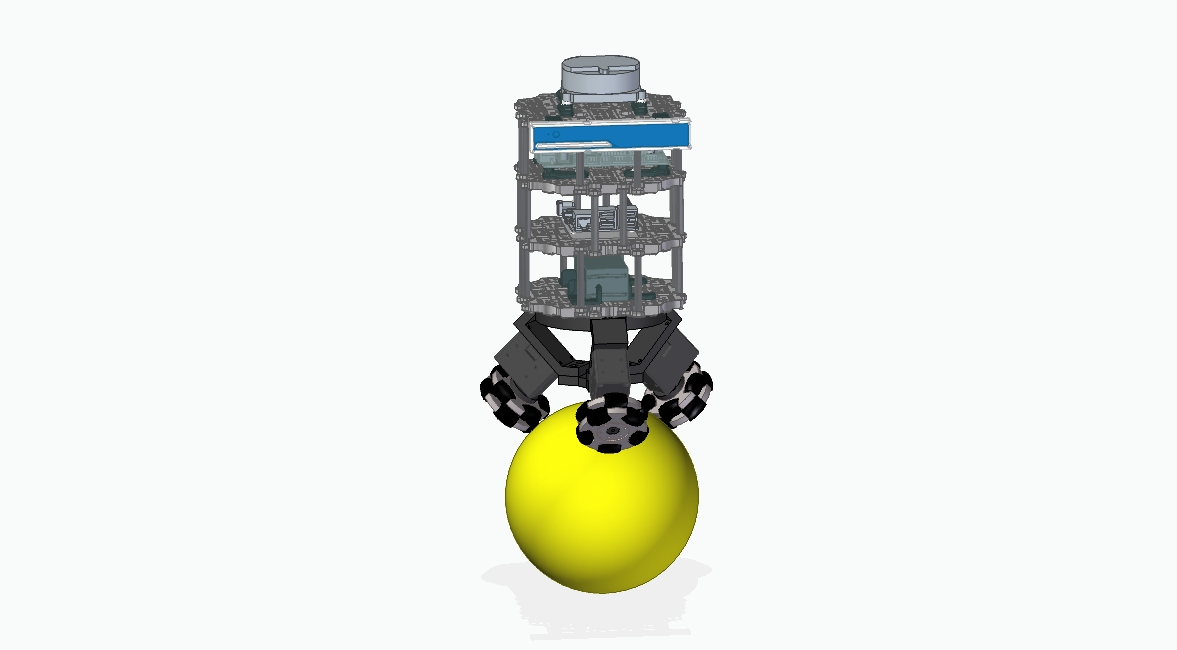
\includegraphics[scale=6.4]{Bilder/Michael/TUD_Ballbot_V30_MS_mit_Raeder_BAll.jpg} }
	\caption{Oberbau, bestehend aus vier Etagen}
	\label{fig:oberbau}
\end{figure}

F�r den Entwurf eines auf einem Ball balancierenden Roboters kann das System zur Vereinfachung als ein inverses Pendel betrachtet werden, dessen Drehachse auf einer beweglichen Plattform gelagert ist. Dies ist in Abbildung \ref{fig:invPendulum} beispielhaft dargestellt. Unter dieser Annahme k�nnen erste Absch�tzungen �ber das dynamische Verhalten getroffen werden. Aus der Anschauung heraus kann direkt gefolgert werden, dass der Pendelarm mit der L�nge $l$ einen Einfluss auf die Pendeldynamik des Systems haben muss. Leitet man nun wie in \cite{pendel}, unter Verwendung der Momentenbilanz das nichtlineare Differenzialgleichungssstem zweiter Ordnung des Auslenkwinkels $\vartheta$ sowie der Schlittenstrecke $x_w$ her, so erh�lt man die Gleichungen: 

        \begin{align} \label{eq:InvPendelThetaDotDot}
            \ddot{\vartheta} &= \frac{l\cdot m}{I}\cdot [-\cos{\vartheta} \cdot \ddot{x}_{w}+g\cdot  \sin{\vartheta}] ,\\   
            \label{eq:InvPendelXDotDot}
            \ddot{x}_w &= \frac{F_{motor}-F_{Reib}}{M+m} + \frac{m\cdot l}{M+m}\dot{\vartheta}^2 \cdot \sin{\vartheta} - \ddot{\vartheta}\cdot cos(\vartheta) . 
        \end{align}


Setzt man nun das Massentr�gheitsmoment des inversen Pendels

        \begin{align} \label{eq:tr�gheitsmoment}
            I &= \frac{4}{3}m\cdot l^2 ,   
        \end{align}
in Gl.\,\ref{eq:InvPendelThetaDotDot} ein, so ergibt sich:  

        \begin{align} \label{eq:InvPendelThetaDotDot_Neu}
            \ddot{\vartheta} &= \frac{3}{4\cdot l}\cdot[-\cos{\vartheta} \cdot \ddot{x}_w+g \cdot  \sin{\vartheta}] . 
        \end{align}

\begin{figure}[H]%
	\centering
	{ \scalebox{1}{{\input{./Bilder/Michael/Schlitten.pdf_tex}}}}%
	\caption{Darstellung eines Ballbots als inverses Pendel}%
	\label{fig:invPendulum}%
\end{figure}%\newline

Anhand der Gleichung (\ref{eq:InvPendelThetaDotDot_Neu}) l�sst sich wie bereits vermutet eine Abh"angikeit der Winkelbeschleunigung $\ddot{\vartheta}$ von der Hebelarml"ange $l$ erkennen. Da sich die Hebelarml�nge jedoch aus der Distanz zwischen Drehachse und Massenschwerpunkt zusammensetzt, bestimmt die Verteilung der Ballbotmasse die Hebelarml�nge des inversen Pendels. Durch das Vergr��ern der Hebelarml�nge $l$ kann so die Winkelbeschleunigung $\ddot{\vartheta}$ f�r kleine Winkelauslenkungen $\Delta \vartheta$ verringert werden. Dadurch ist das System leichter zu stabilisieren. Bei Betrachtung der Gleichung (\ref{eq:InvPendelXDotDot}) l�sst sich jedoch erkennen, dass mit einer Verl�ngerung des Hebelarms $l$ eine gr��ere Beschleunigung $\ddot{x}_w$  des Schlittens einhergehen muss, die durch entsprechend starke Drehmomente realisiert werden kann.

Wendet man dieses Prinzip eines gro�en Hebelarms auf den Ballbot an, so stellt sich jedoch heraus, dass es nur bedingt anwendbar ist. Ursache hierf�r ist die Schnittstelle zwischen omnidirektionalen R�dern und Ball, da hier aufgrund des Reibkoeffizienten nur ein begrenztes Drehmoment �bertragen werden kann. Der Reibkoeffizient begrenzt somit die gew�nschte Sollbeschleunigung des Balles. 

Da eine optimale Auslegung der Pendelarml�nge rechnerisch nur schwer zu bestimmen ist, w�re es w�nschenswert, die Hebelarml�nge durch eine flexible Hardware ver�ndern zu k�nnen. Durch das Hinzuf�gen bzw. Entfernen von weiteren Ebenen im Aufbau des Ballbots kann der Massenschwerpunkt und somit die Pendelarml�nge des Ballbots variabel eingestellt werden. So kann die optimale Konfiguration sehr einfach experimentell bestimmt werden. 

Als Hardware f�r den Ballbot hat man sich daher f�r das TurtleBot3-Paket in der Burger-Variante entschieden. Auf diese soll im Kapitel \ref{sec:Hardware} tiefer eingegangen werden. Bei der Wahl des Balles sowie der Antriebsanordnung hat man sich die Konzepte bereits funktionierender Ballbots als Grundlage hergenommen. Die folgenden Kapitel gehen dabei n�her auf die einzelnen Konstruktionsschritte ein. 

\section{Verwendete Hardware} \label{sec:Hardware}
 Beim Entwurf des Ballbots wurde, wie bereits erw�hnt, auf die leistungsf"ahige Hardware eines TurtleBot3 in der \glqq Burger\grqq-Variante zur"uck gegriffen. Dieses Paket umfasst neben einem robusten mechanischen Aufbau auch alle grundlegenden elektronischen Komponenten wie Sensoren, Mikrocontrollern und Antriebseinheiten, die f�r die Entwicklung eines auf einem Ball balancierenden Roboters ben�tigt werden. Die wichtigsten Komponenten werden in den nachfolgenden Unterkapitel n�her erl�utert.

\subsection{OpenCR-Board} \label{sec:openCr}

Das im Projekt verwendete OpenCR-Board (in der Version 1.0), wie in Abbildung \ref{fig:opencr_board} dargestellt, ist ein Mikrocontroller, der f�r Roboterprojekte in der Gr��e des TurtleBot3-Pakets perfekt geeignet ist. Das gesamte Board, von der Hardware bis zur Software, ist durch Open-Source-Lizenzen frei verf�gbar. Es bietet mit insgesamt 10 verschiedenen Kommunikationsstellen und einer integrierten inertialen Messeinheit (IMU)\footnote{Die verwendete IMU ist die MPU-9250 siehe \url{https://www.invensense.com/products/motion-tracking/9-axis/mpu-9250/}.} bei der Entwicklung von Robotersystemen. Dar�ber hinaus ist das OpenCR-Board mit einem leistungsstarken ARM Cortex-M7 Prozessor ausgestattet.

\begin{figure}[H]%H !htbp
	\centering
	{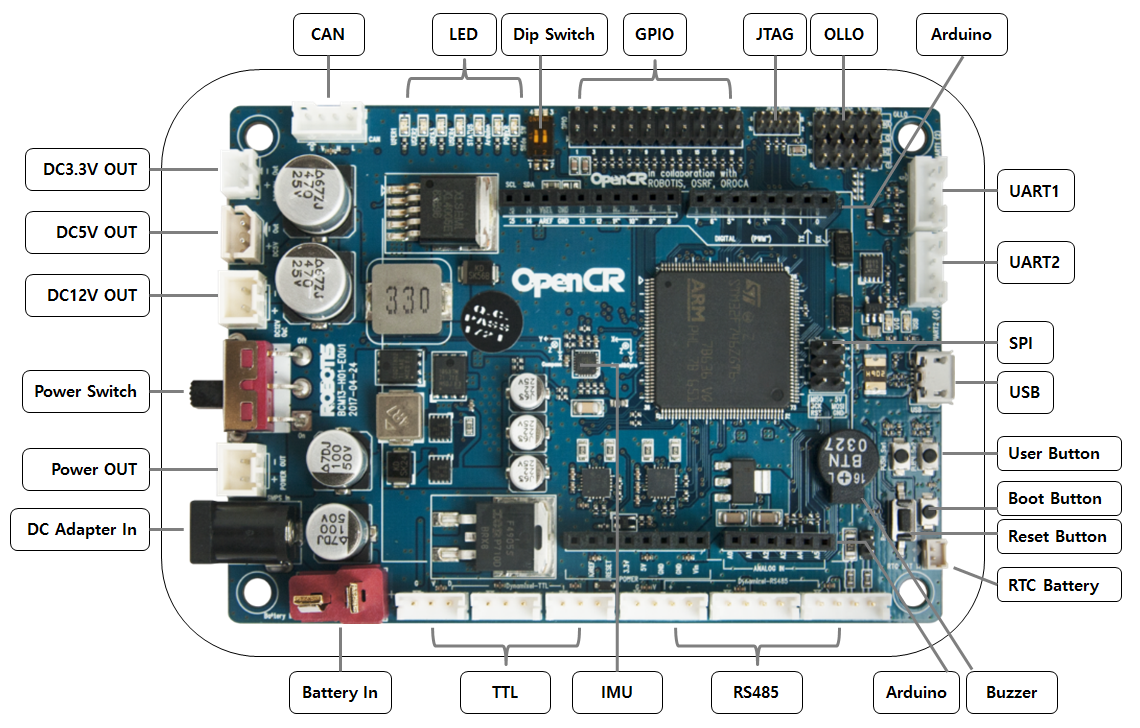
\includegraphics[scale=0.45]{Bilder/Michael/opencr.png} }
	\caption{�bersicht der Schnittstellen des OpenCR-Boards \cite{openCR}}
	\label{fig:opencr_board}
\end{figure}

%https://github.com/ROBOTIS-GIT/emanual/blob/master/docs/en/platform/turtlebot3/appendix_opencr1_0.md

\subsection{Sensorik} \label{sec:sensoren}
Am Ballbot wurden mehrere Sensoren verbaut, die f�r verschiedene Aufgabenbereiche ben�tigt werden. Tabelle \ref{tab:sensoren} zeigt dabei eine �bersicht der Sensoren, die zur Stabilisierung bzw. zur Lokalisation verwendet werden.  


\begin{table}[H]
	\caption["Ubersicht Sensoren]{Sensoren, die im Ballbot verbaut wurden} \label{tab:sensoren}
  		\begin{center}				
		\begin{longtable}{|c||c|c|c|}
		\hline 
  		\multicolumn{4}{|c|}{�bersicht Sensoren} \\ 
  		\hline
  		Kategorie & Stabilisierung & \multicolumn{2}{c|}{Lokalisierung/Interaktion} \\ 
  		\hline
  		\hline
  		Bezeichnung & IMU & Kamera & Laser Distance Sensor\\
  		& MPU-9250 & Intel Realsense R200 & LDS-01\\
  		\hline	\hline
  		
  		 & & & \\
         Taktfrequenz: & 4Hz - 8kHz & 2.5GHz & 1,8 kHz\\
         & & & \\
         Features: & Gyroskop & IR Laser Projector System & DA: 120mm - 3500mm\\
                  & Accelerometer & Full HD RGB Color Stream & Scan Rate: 300$\pm$10 rpm\\
                  & Magnetometer & Onboard Imaging ASIC & Angular Resolution: $1^{\circ}$\\	
  		\hline
		\end{longtable}
  		\end{center}
\end{table} 


\subsection{Motoren} \label{sec:Motoren}

\begin{figure}[H]%
	\centering
	{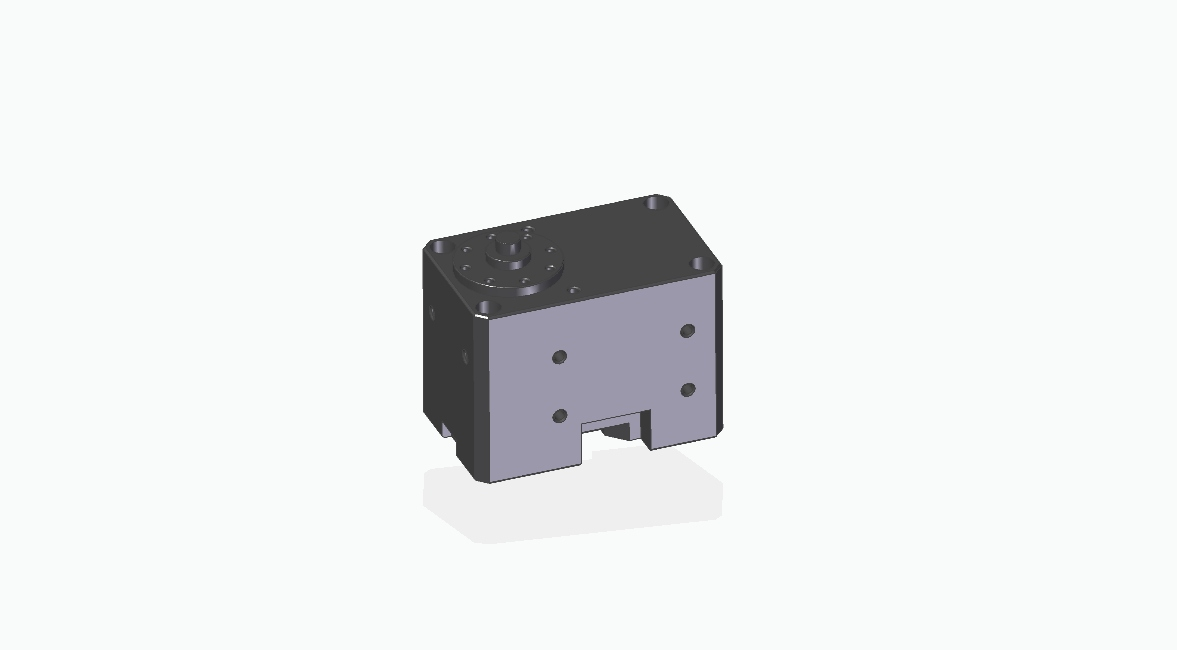
\includegraphics[scale=6.4]{Bilder/Michael/Motoren.jpg} }
	\caption{Motorenspezifikationen}
	\label{fig:motorenspezifikationen}
\end{figure}


Im TurtleBot3-Paket enthalten sind weiterhin auch die Motoren, welche f"ur den Ballbotaufbau verwendet werden. Es handelt sich dabei um Dynamixel Servomotoren der Baureihe XM430-W350-T. Die Motoren haben sich als sehr robust erwiesen und k"onnen durch eine hohe "Ubersetzung von $i=1:353.5$ ein variables ausgangsseitiges Drehmoment von bis zu $3.8$\,Nm bei $11.1$\,V \cite{XM430} erzeugen. Dies ist f"ur die gegebenen Systemkonfiguration mehr als ausreichend. Weiterhin werden von Dynamixel bereits verschiedene Betriebsarten bereitgestellt, in denen die Motoren betrieben werden k"onnen. So bieten die Motoren neben einer Positionsregelung, einer Geschwindigkeitsregelung auch eine Stromregelung. Durch die lineare Abh"angikeit zwischen Drehmoment und Strom kann somit das abtriebseitige Drehmoment geregelt werden.
 
Vom OpenCR-Board werden mittels dem RS485-Protokoll sogennante Units �bertragen. Die Units werden dann intern im Motor in einen realen Sollstrom umgewandelt. Der Strom kann �ber die Formel 

\begin{align} \label{eq:CurrentUnit}
I &= k_{unit}\cdot Units, && \text{mit}  & k_{unit} &= 2,69\cdot 10^{-3} \frac{A}{Unit}
\end{align}

berechnet werden. Anschlie�end kann mit Hilfe der Drehmoment(Nm)-Strom(A)-Kennlinie aus dem Datenblatt \cite{XM430} die spezifische Motorkonstante zu $k_{motor} = 1,63$\,Nm/A bestimmt werden.  
  bestimmt.  Dadurch kann das vom Motor erzeugte Drehmoment aus den Units mittels der Formel 
  \begin{align} \label{eq:CurrentTorque}
  M &= k_{motor} \cdot I \\
    &= k_{motor}\cdot k_{unit} \cdot Units
  \end{align}
  berechnet werden. Insgesamt ergibt sich folgender Gesamtumrechnungsfaktor 
    \begin{align} \label{eq:CurrentTorque}
    k &= k_{motor}\cdot k_{unit} = 228\cdot \frac{Nm}{Unit} 
    \end{align}
    
In der technischen Umsetzung hat sich herausgestellt, dass die Motoren zueinander ein unterschiedliches Verhalten aufweisen und somit die Konstante $k$ nicht f�r alle drei Motoren verwendet werden kann. Daher wurde die Konstante $k$ experimentell bestimmt.
Hierzu wird ein Pr�fhebel der L�nge $l_{pruef}$ f�r die Motoren konstruiert, der w�hrend des Betriebs der Motoren auf eine Waage dr�ckt. Die Motoren werden mit einer bestimmten Folge von dimensionslosen Einheiten angesteuert und jeweils das angezeigte Gewicht der Waage $m$ notiert.
Mit der Beziehung
\begin{align} \label{eq:FMG}
F &= m \cdot g \nonumber
\end{align}
eingesetzt in
\begin{align} 
 M &= F \cdot l_{\text{pruef}}
\end{align}
kann das resultierende Drehmoment $M$ berechnet werden und somit die Konstante $k$ f�r jeden einzelnen Motor.

Bei den Messungen wurde festgestellt, dass das von den Motoren erzeugte Drehmoment einen Drift\footnote{Unter einem Drift ist hier gemeint, dass bei konstantem Anlegen von Units (Stromwert) das Drehmoment �ber die Zeit abnimmt.} aufweist. Dieser Drift konnte reduziert werden, in dem man statt einmaligen Drehmomentbefehlen, die Befehle in Form einer Pulsung wiederkehrend an den Motor �bergeben hat. Die neuen $k$-Faktoren sind �ber die Ergebnisse der Messungen, dargestellt in den Abbildungen \ref{fig:Motorkonstante1}, \ref{fig:Motorkonstante2} und \ref{fig:Motorkonstante3}, mittels der Methode der kleinsten Quadrate berechnet worden. Aus diesen Abbildungen ist zu erkennen, dass sich die Drehmoment-Unit-Konstanten f�r die einzelnen baugleichen Motoren unterscheiden. Dieses Verhalten wurde bei der Implementierung in Kapitel \ref{ch:Implementierung} ber�cksichtigt.
\begin{figure}[!htbp]%
	\centering
	{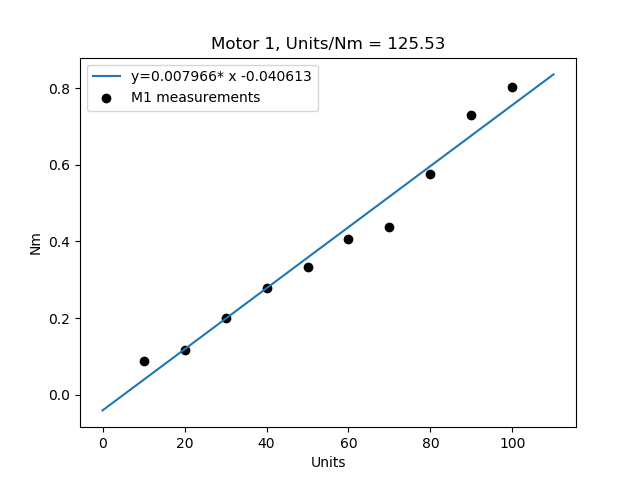
\includegraphics[scale=0.55]{Bilder/Michael/Motor1.png} }
	\caption{Bestimmung der Drehmoment-Unit-Konstante f�r Motor 1}
	\label{fig:Motorkonstante1}
\end{figure}

\begin{figure}[!htbp]%
	\centering
	{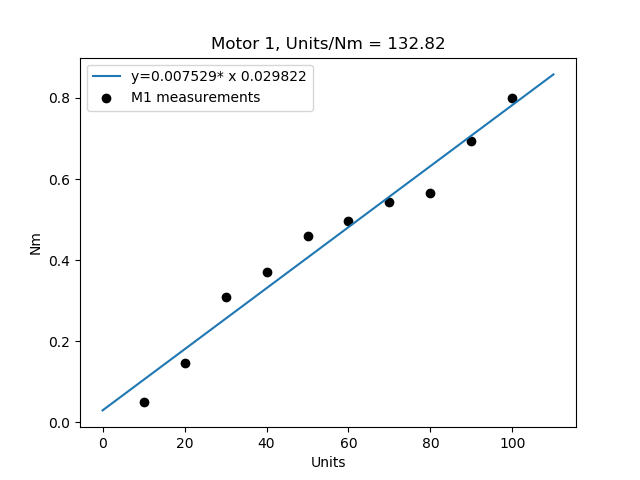
\includegraphics[scale=0.55]{Bilder/Michael/Motor2.png} }
	\caption{Bestimmung der Drehmoment-Unit-Konstante f�r Motor 2}
	\label{fig:Motorkonstante2}
\end{figure}

\begin{figure}[!htbp]%
	\centering
	{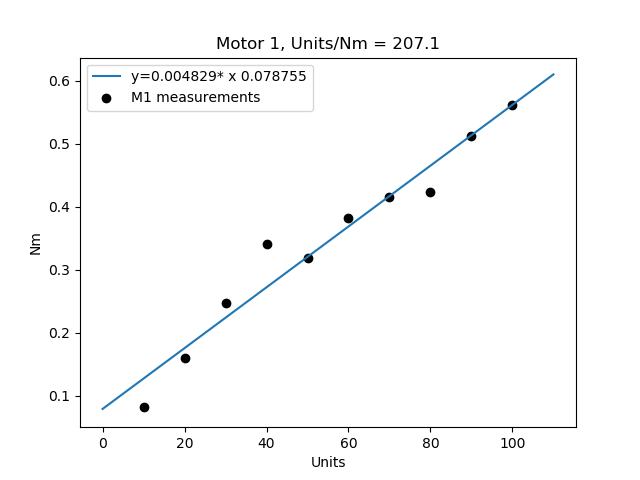
\includegraphics[scale=0.55]{Bilder/Michael/Motor3.png} }
	\caption{Bestimmung der Drehmoment-Unit-Konstante f�r Motor 3}
	\label{fig:Motorkonstante3}
\end{figure}      
            
\section{Ballbot-Design} \label{sec:entwurf}
Die mechanische Systemkonfiguration kann in drei Teile untergliedert werden. Dies ist zum einen der Oberbau (Kap.\ref{sec:oberbau}), der Unterbau (Kap.\ref{sec:unterbau}) sowie der Ball (Kap.\ref{sec:ball}), auf dem das Gesamtsystem bestehend aus Ober- und Unterbau balancieren wird. Nachfolgende Kapitel dokumentieren die Entwicklungsprozesse der einzelnen Teile. 

\subsection{Oberbau} \label{sec:oberbau}

\begin{figure}[H]%
	\centering
	{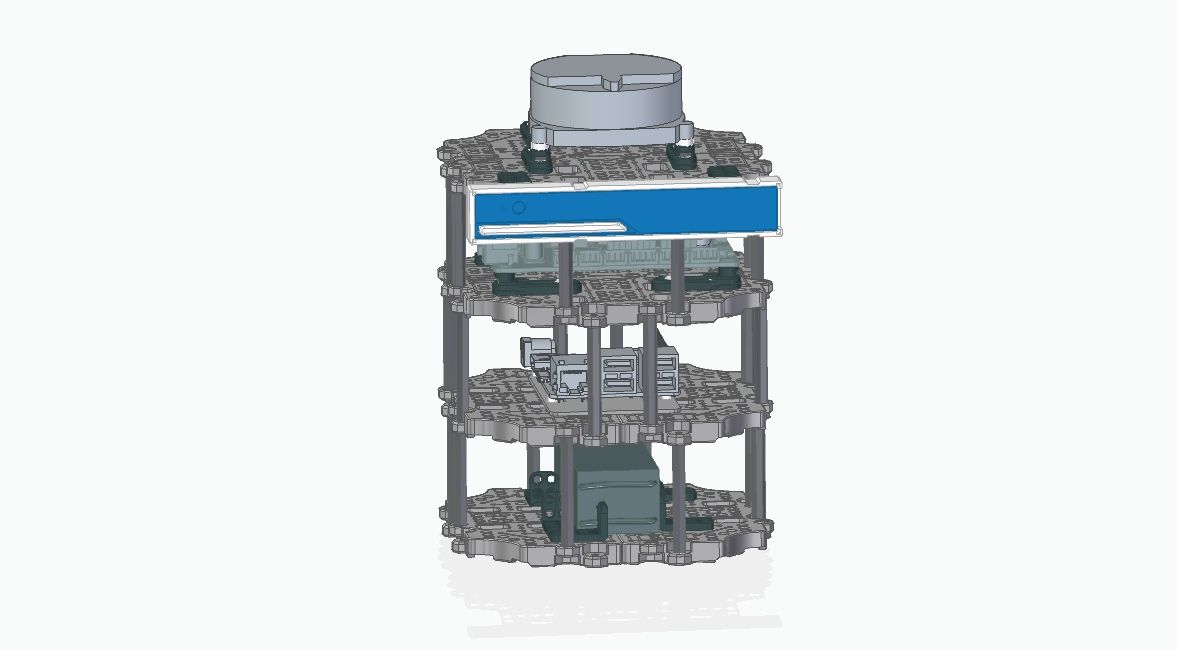
\includegraphics[scale=6.4]{Bilder/Michael/Oberbau.jpg} }
	\caption{Oberbau, bestehend aus vier Etagen}
	\label{fig:oberbau}
\end{figure}

Die Konfiguration des Oberbaus hat sich experimentell unter Ber�cksichtigung der in Kapitel \ref{ch:Modellierung} hergeleiteten Beziehungen ergeben. In der untersten Ebene ist die Batterie platziert. Dar�ber folgt eine Ebene mit einem Up-Level Computer, der f�r rechenintensiver Aufgaben wie der Lokalisation ben�tigt wird. Dieser wird jedoch in dieser Arbeit nicht weiter ber�cksichtigt. Anschlie�end folgt das OpenCR-Board mit den dar�ber platzierten Sensoren zur Lokalisierung des Roboters im Raum, vgl. Abbildung \ref{fig:oberbau}. 


\subsection{Unterbau} \label{sec:unterbau}

\begin{figure}[htb!]%
	\centering
	{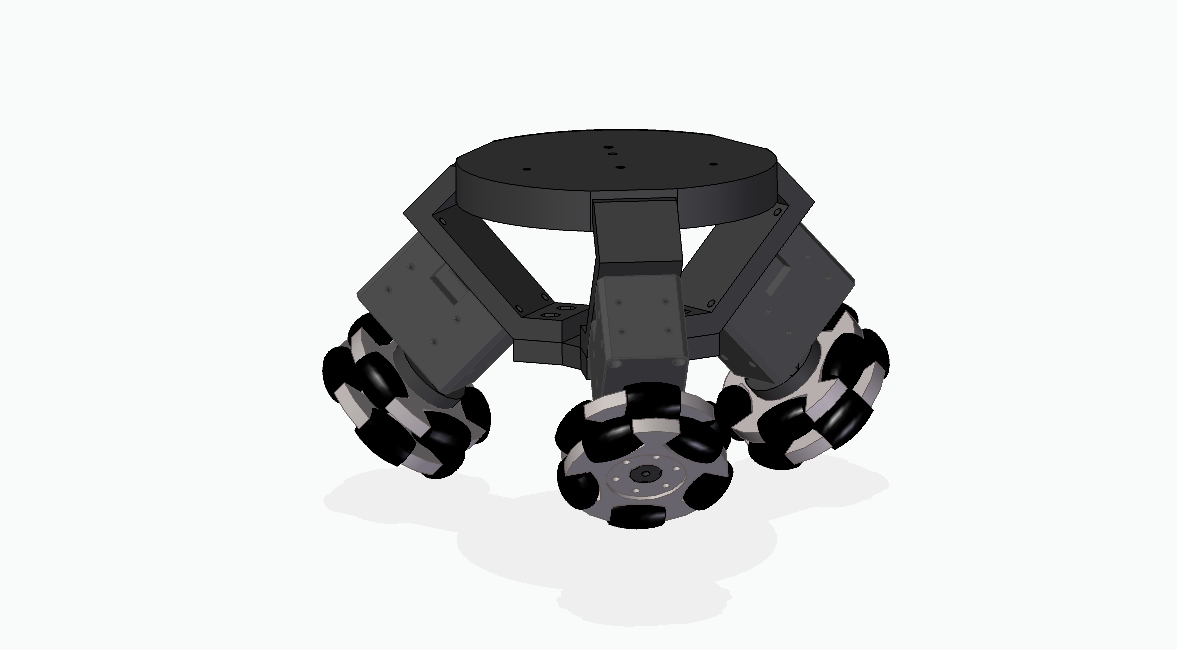
\includegraphics[scale=6.4]{Bilder/Michael/Unterbau.jpg} }
	\caption{Unterbau}
	\label{fig:Unterbau}
\end{figure}

Die Aufgabe des Unterbaus besteht in der Positionierung der Antriebe. Dabei sollte dieser m�glichst leicht und zugleich stabil konstruiert werden. 

Damit das Drehmoment der Motoren optimal auf den Ball �bertragen werden kann, m�ssen die R�der gegen�ber der z-Achse\footnote{Die z-Achse ist die zum Ballbot vertikale Achse.} des Ballbots einen Winkel von $\alpha=45^{\circ}$ einschlie�en. Weiterhin wurden die R�der um einen Winkel von $\beta=120^{\circ}$ zueinander versetzt befestigt. Diese konstruktionsbedingten Winkel sind in Abbildung \ref{fig:konstruktions�bersicht} dargestellt.

\begin{figure}[H]%
	\centering
	{ \scalebox{1}{{\chapter{Konstruktion} \label{ch:konstruktion}

\section{Konzeptionierung} \label{sec:konzeptionierung}

\begin{figure}[H]%
	\centering
	{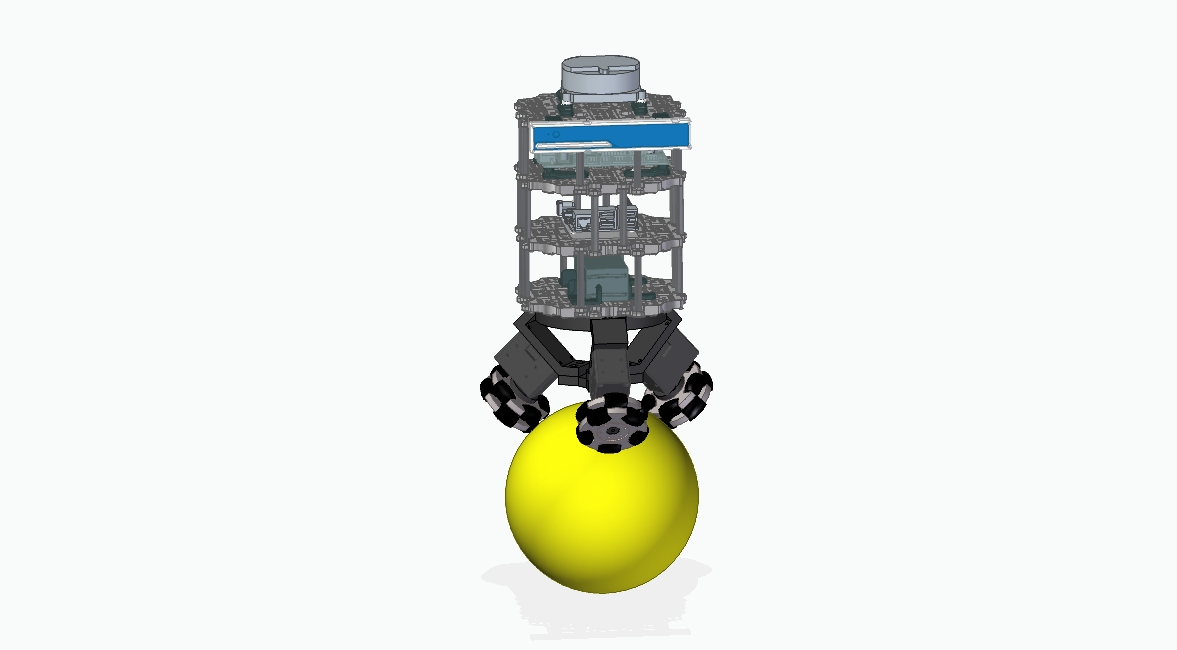
\includegraphics[scale=6.4]{Bilder/Michael/TUD_Ballbot_V30_MS_mit_Raeder_BAll.jpg} }
	\caption{Oberbau, bestehend aus vier Etagen}
	\label{fig:oberbau}
\end{figure}

F�r den Entwurf eines auf einem Ball balancierenden Roboters kann das System zur Vereinfachung als ein inverses Pendel betrachtet werden, dessen Drehachse auf einer beweglichen Plattform gelagert ist. Dies ist in Abbildung \ref{fig:invPendulum} beispielhaft dargestellt. Unter dieser Annahme k�nnen erste Absch�tzungen �ber das dynamische Verhalten getroffen werden. Aus der Anschauung heraus kann direkt gefolgert werden, dass der Pendelarm mit der L�nge $l$ einen Einfluss auf die Pendeldynamik des Systems haben muss. Leitet man nun wie in \cite{pendel}, unter Verwendung der Momentenbilanz das nichtlineare Differenzialgleichungssstem zweiter Ordnung des Auslenkwinkels $\vartheta$ sowie der Schlittenstrecke $x_w$ her, so erh�lt man die Gleichungen: 

        \begin{align} \label{eq:InvPendelThetaDotDot}
            \ddot{\vartheta} &= \frac{l\cdot m}{I}\cdot [-\cos{\vartheta} \cdot \ddot{x}_{w}+g\cdot  \sin{\vartheta}] ,\\   
            \label{eq:InvPendelXDotDot}
            \ddot{x}_w &= \frac{F_{motor}-F_{Reib}}{M+m} + \frac{m\cdot l}{M+m}\dot{\vartheta}^2 \cdot \sin{\vartheta} - \ddot{\vartheta}\cdot cos(\vartheta) . 
        \end{align}


Setzt man nun das Massentr�gheitsmoment des inversen Pendels

        \begin{align} \label{eq:tr�gheitsmoment}
            I &= \frac{4}{3}m\cdot l^2 ,   
        \end{align}
in Gl.\,\ref{eq:InvPendelThetaDotDot} ein, so ergibt sich:  

        \begin{align} \label{eq:InvPendelThetaDotDot_Neu}
            \ddot{\vartheta} &= \frac{3}{4\cdot l}\cdot[-\cos{\vartheta} \cdot \ddot{x}_w+g \cdot  \sin{\vartheta}] . 
        \end{align}

\begin{figure}[H]%
	\centering
	{ \scalebox{1}{{\input{./Bilder/Michael/Schlitten.pdf_tex}}}}%
	\caption{Darstellung eines Ballbots als inverses Pendel}%
	\label{fig:invPendulum}%
\end{figure}%\newline

Anhand der Gleichung (\ref{eq:InvPendelThetaDotDot_Neu}) l�sst sich wie bereits vermutet eine Abh"angikeit der Winkelbeschleunigung $\ddot{\vartheta}$ von der Hebelarml"ange $l$ erkennen. Da sich die Hebelarml�nge jedoch aus der Distanz zwischen Drehachse und Massenschwerpunkt zusammensetzt, bestimmt die Verteilung der Ballbotmasse die Hebelarml�nge des inversen Pendels. Durch das Vergr��ern der Hebelarml�nge $l$ kann so die Winkelbeschleunigung $\ddot{\vartheta}$ f�r kleine Winkelauslenkungen $\Delta \vartheta$ verringert werden. Dadurch ist das System leichter zu stabilisieren. Bei Betrachtung der Gleichung (\ref{eq:InvPendelXDotDot}) l�sst sich jedoch erkennen, dass mit einer Verl�ngerung des Hebelarms $l$ eine gr��ere Beschleunigung $\ddot{x}_w$  des Schlittens einhergehen muss, die durch entsprechend starke Drehmomente realisiert werden kann.

Wendet man dieses Prinzip eines gro�en Hebelarms auf den Ballbot an, so stellt sich jedoch heraus, dass es nur bedingt anwendbar ist. Ursache hierf�r ist die Schnittstelle zwischen omnidirektionalen R�dern und Ball, da hier aufgrund des Reibkoeffizienten nur ein begrenztes Drehmoment �bertragen werden kann. Der Reibkoeffizient begrenzt somit die gew�nschte Sollbeschleunigung des Balles. 

Da eine optimale Auslegung der Pendelarml�nge rechnerisch nur schwer zu bestimmen ist, w�re es w�nschenswert, die Hebelarml�nge durch eine flexible Hardware ver�ndern zu k�nnen. Durch das Hinzuf�gen bzw. Entfernen von weiteren Ebenen im Aufbau des Ballbots kann der Massenschwerpunkt und somit die Pendelarml�nge des Ballbots variabel eingestellt werden. So kann die optimale Konfiguration sehr einfach experimentell bestimmt werden. 

Als Hardware f�r den Ballbot hat man sich daher f�r das TurtleBot3-Paket in der Burger-Variante entschieden. Auf diese soll im Kapitel \ref{sec:Hardware} tiefer eingegangen werden. Bei der Wahl des Balles sowie der Antriebsanordnung hat man sich die Konzepte bereits funktionierender Ballbots als Grundlage hergenommen. Die folgenden Kapitel gehen dabei n�her auf die einzelnen Konstruktionsschritte ein. 

\section{Verwendete Hardware} \label{sec:Hardware}
 Beim Entwurf des Ballbots wurde, wie bereits erw�hnt, auf die leistungsf"ahige Hardware eines TurtleBot3 in der \glqq Burger\grqq-Variante zur"uck gegriffen. Dieses Paket umfasst neben einem robusten mechanischen Aufbau auch alle grundlegenden elektronischen Komponenten wie Sensoren, Mikrocontrollern und Antriebseinheiten, die f�r die Entwicklung eines auf einem Ball balancierenden Roboters ben�tigt werden. Die wichtigsten Komponenten werden in den nachfolgenden Unterkapitel n�her erl�utert.

\subsection{OpenCR-Board} \label{sec:openCr}

Das im Projekt verwendete OpenCR-Board (in der Version 1.0), wie in Abbildung \ref{fig:opencr_board} dargestellt, ist ein Mikrocontroller, der f�r Roboterprojekte in der Gr��e des TurtleBot3-Pakets perfekt geeignet ist. Das gesamte Board, von der Hardware bis zur Software, ist durch Open-Source-Lizenzen frei verf�gbar. Es bietet mit insgesamt 10 verschiedenen Kommunikationsstellen und einer integrierten inertialen Messeinheit (IMU)\footnote{Die verwendete IMU ist die MPU-9250 siehe \url{https://www.invensense.com/products/motion-tracking/9-axis/mpu-9250/}.} bei der Entwicklung von Robotersystemen. Dar�ber hinaus ist das OpenCR-Board mit einem leistungsstarken ARM Cortex-M7 Prozessor ausgestattet.

\begin{figure}[H]%H !htbp
	\centering
	{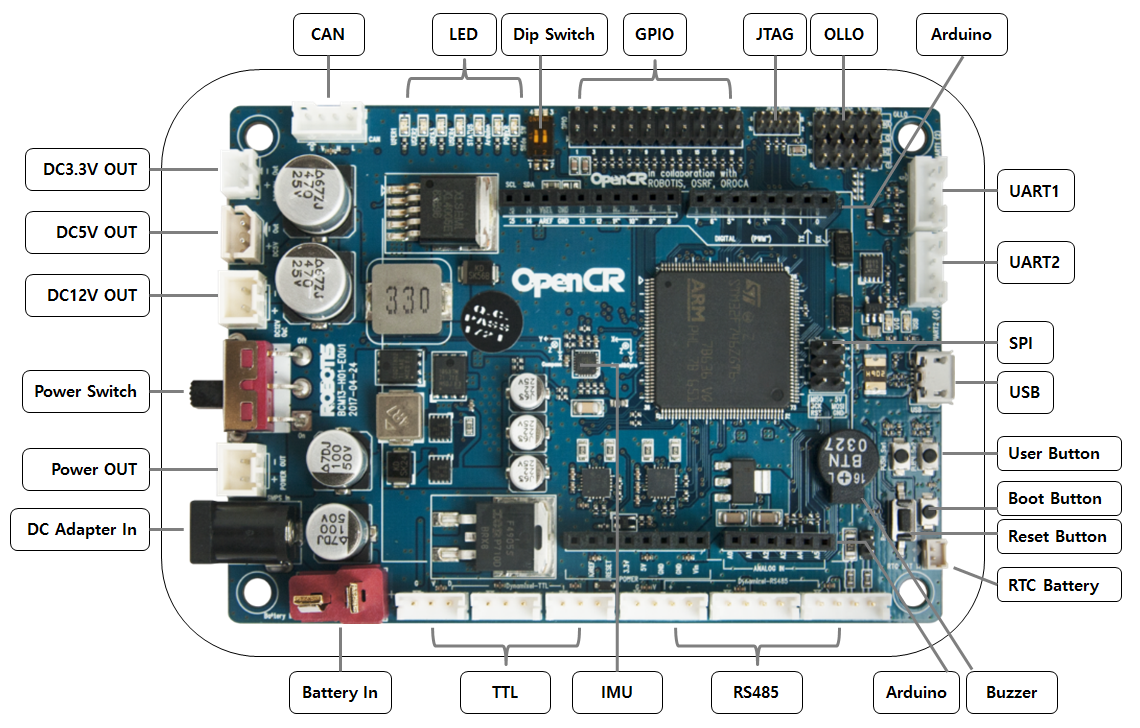
\includegraphics[scale=0.45]{Bilder/Michael/opencr.png} }
	\caption{�bersicht der Schnittstellen des OpenCR-Boards \cite{openCR}}
	\label{fig:opencr_board}
\end{figure}

%https://github.com/ROBOTIS-GIT/emanual/blob/master/docs/en/platform/turtlebot3/appendix_opencr1_0.md

\subsection{Sensorik} \label{sec:sensoren}
Am Ballbot wurden mehrere Sensoren verbaut, die f�r verschiedene Aufgabenbereiche ben�tigt werden. Tabelle \ref{tab:sensoren} zeigt dabei eine �bersicht der Sensoren, die zur Stabilisierung bzw. zur Lokalisation verwendet werden.  


\begin{table}[H]
	\caption["Ubersicht Sensoren]{Sensoren, die im Ballbot verbaut wurden} \label{tab:sensoren}
  		\begin{center}				
		\begin{longtable}{|c||c|c|c|}
		\hline 
  		\multicolumn{4}{|c|}{�bersicht Sensoren} \\ 
  		\hline
  		Kategorie & Stabilisierung & \multicolumn{2}{c|}{Lokalisierung/Interaktion} \\ 
  		\hline
  		\hline
  		Bezeichnung & IMU & Kamera & Laser Distance Sensor\\
  		& MPU-9250 & Intel Realsense R200 & LDS-01\\
  		\hline	\hline
  		
  		 & & & \\
         Taktfrequenz: & 4Hz - 8kHz & 2.5GHz & 1,8 kHz\\
         & & & \\
         Features: & Gyroskop & IR Laser Projector System & DA: 120mm - 3500mm\\
                  & Accelerometer & Full HD RGB Color Stream & Scan Rate: 300$\pm$10 rpm\\
                  & Magnetometer & Onboard Imaging ASIC & Angular Resolution: $1^{\circ}$\\	
  		\hline
		\end{longtable}
  		\end{center}
\end{table} 


\subsection{Motoren} \label{sec:Motoren}

\begin{figure}[H]%
	\centering
	{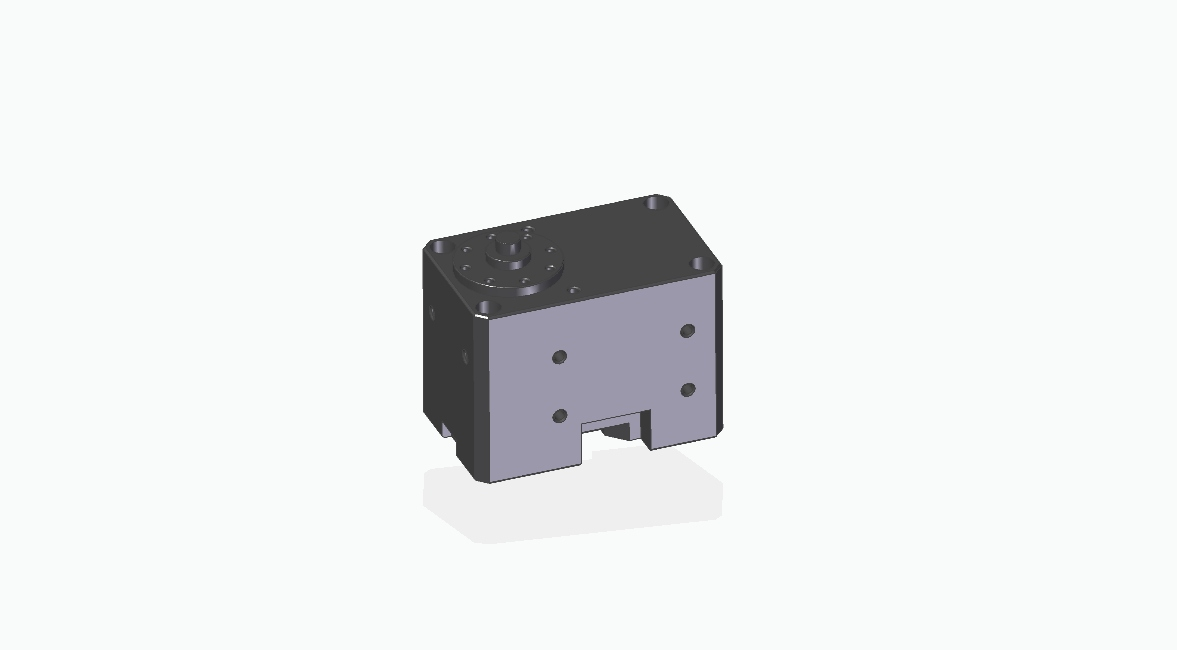
\includegraphics[scale=6.4]{Bilder/Michael/Motoren.jpg} }
	\caption{Motorenspezifikationen}
	\label{fig:motorenspezifikationen}
\end{figure}


Im TurtleBot3-Paket enthalten sind weiterhin auch die Motoren, welche f"ur den Ballbotaufbau verwendet werden. Es handelt sich dabei um Dynamixel Servomotoren der Baureihe XM430-W350-T. Die Motoren haben sich als sehr robust erwiesen und k"onnen durch eine hohe "Ubersetzung von $i=1:353.5$ ein variables ausgangsseitiges Drehmoment von bis zu $3.8$\,Nm bei $11.1$\,V \cite{XM430} erzeugen. Dies ist f"ur die gegebenen Systemkonfiguration mehr als ausreichend. Weiterhin werden von Dynamixel bereits verschiedene Betriebsarten bereitgestellt, in denen die Motoren betrieben werden k"onnen. So bieten die Motoren neben einer Positionsregelung, einer Geschwindigkeitsregelung auch eine Stromregelung. Durch die lineare Abh"angikeit zwischen Drehmoment und Strom kann somit das abtriebseitige Drehmoment geregelt werden.
 
Vom OpenCR-Board werden mittels dem RS485-Protokoll sogennante Units �bertragen. Die Units werden dann intern im Motor in einen realen Sollstrom umgewandelt. Der Strom kann �ber die Formel 

\begin{align} \label{eq:CurrentUnit}
I &= k_{unit}\cdot Units, && \text{mit}  & k_{unit} &= 2,69\cdot 10^{-3} \frac{A}{Unit}
\end{align}

berechnet werden. Anschlie�end kann mit Hilfe der Drehmoment(Nm)-Strom(A)-Kennlinie aus dem Datenblatt \cite{XM430} die spezifische Motorkonstante zu $k_{motor} = 1,63$\,Nm/A bestimmt werden.  
  bestimmt.  Dadurch kann das vom Motor erzeugte Drehmoment aus den Units mittels der Formel 
  \begin{align} \label{eq:CurrentTorque}
  M &= k_{motor} \cdot I \\
    &= k_{motor}\cdot k_{unit} \cdot Units
  \end{align}
  berechnet werden. Insgesamt ergibt sich folgender Gesamtumrechnungsfaktor 
    \begin{align} \label{eq:CurrentTorque}
    k &= k_{motor}\cdot k_{unit} = 228\cdot \frac{Nm}{Unit} 
    \end{align}
    
In der technischen Umsetzung hat sich herausgestellt, dass die Motoren zueinander ein unterschiedliches Verhalten aufweisen und somit die Konstante $k$ nicht f�r alle drei Motoren verwendet werden kann. Daher wurde die Konstante $k$ experimentell bestimmt.
Hierzu wird ein Pr�fhebel der L�nge $l_{pruef}$ f�r die Motoren konstruiert, der w�hrend des Betriebs der Motoren auf eine Waage dr�ckt. Die Motoren werden mit einer bestimmten Folge von dimensionslosen Einheiten angesteuert und jeweils das angezeigte Gewicht der Waage $m$ notiert.
Mit der Beziehung
\begin{align} \label{eq:FMG}
F &= m \cdot g \nonumber
\end{align}
eingesetzt in
\begin{align} 
 M &= F \cdot l_{\text{pruef}}
\end{align}
kann das resultierende Drehmoment $M$ berechnet werden und somit die Konstante $k$ f�r jeden einzelnen Motor.

Bei den Messungen wurde festgestellt, dass das von den Motoren erzeugte Drehmoment einen Drift\footnote{Unter einem Drift ist hier gemeint, dass bei konstantem Anlegen von Units (Stromwert) das Drehmoment �ber die Zeit abnimmt.} aufweist. Dieser Drift konnte reduziert werden, in dem man statt einmaligen Drehmomentbefehlen, die Befehle in Form einer Pulsung wiederkehrend an den Motor �bergeben hat. Die neuen $k$-Faktoren sind �ber die Ergebnisse der Messungen, dargestellt in den Abbildungen \ref{fig:Motorkonstante1}, \ref{fig:Motorkonstante2} und \ref{fig:Motorkonstante3}, mittels der Methode der kleinsten Quadrate berechnet worden. Aus diesen Abbildungen ist zu erkennen, dass sich die Drehmoment-Unit-Konstanten f�r die einzelnen baugleichen Motoren unterscheiden. Dieses Verhalten wurde bei der Implementierung in Kapitel \ref{ch:Implementierung} ber�cksichtigt.
\begin{figure}[!htbp]%
	\centering
	{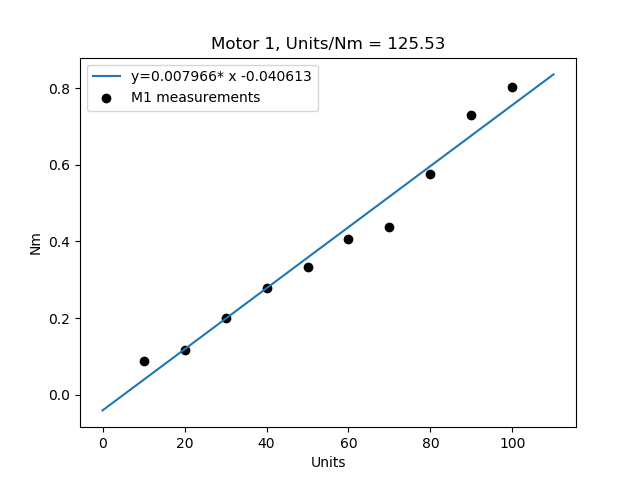
\includegraphics[scale=0.55]{Bilder/Michael/Motor1.png} }
	\caption{Bestimmung der Drehmoment-Unit-Konstante f�r Motor 1}
	\label{fig:Motorkonstante1}
\end{figure}

\begin{figure}[!htbp]%
	\centering
	{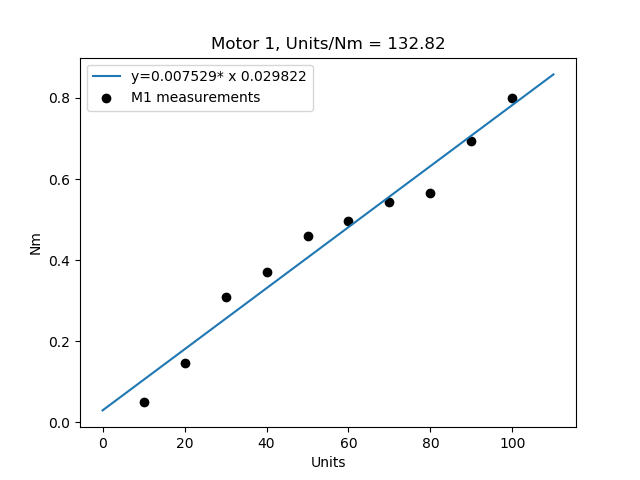
\includegraphics[scale=0.55]{Bilder/Michael/Motor2.png} }
	\caption{Bestimmung der Drehmoment-Unit-Konstante f�r Motor 2}
	\label{fig:Motorkonstante2}
\end{figure}

\begin{figure}[!htbp]%
	\centering
	{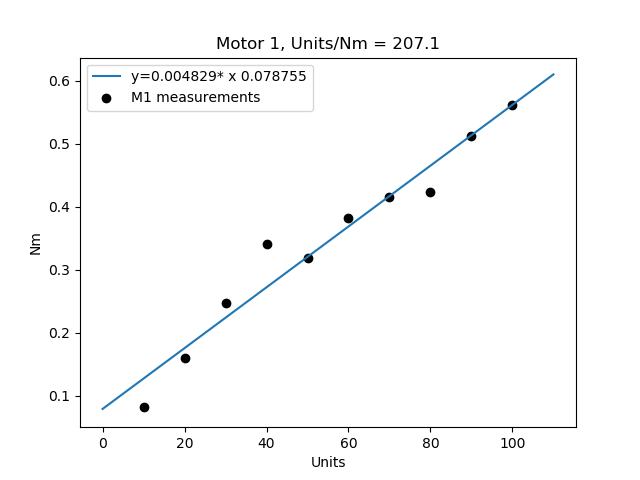
\includegraphics[scale=0.55]{Bilder/Michael/Motor3.png} }
	\caption{Bestimmung der Drehmoment-Unit-Konstante f�r Motor 3}
	\label{fig:Motorkonstante3}
\end{figure}      
            
\section{Ballbot-Design} \label{sec:entwurf}
Die mechanische Systemkonfiguration kann in drei Teile untergliedert werden. Dies ist zum einen der Oberbau (Kap.\ref{sec:oberbau}), der Unterbau (Kap.\ref{sec:unterbau}) sowie der Ball (Kap.\ref{sec:ball}), auf dem das Gesamtsystem bestehend aus Ober- und Unterbau balancieren wird. Nachfolgende Kapitel dokumentieren die Entwicklungsprozesse der einzelnen Teile. 

\subsection{Oberbau} \label{sec:oberbau}

\begin{figure}[H]%
	\centering
	{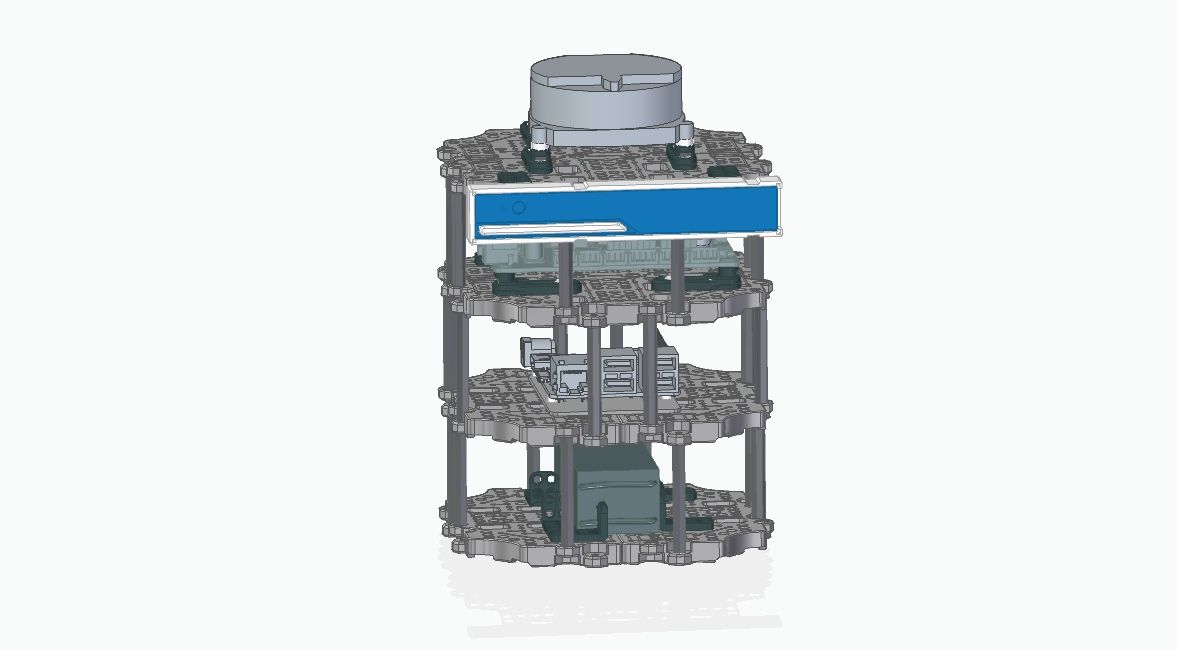
\includegraphics[scale=6.4]{Bilder/Michael/Oberbau.jpg} }
	\caption{Oberbau, bestehend aus vier Etagen}
	\label{fig:oberbau}
\end{figure}

Die Konfiguration des Oberbaus hat sich experimentell unter Ber�cksichtigung der in Kapitel \ref{ch:Modellierung} hergeleiteten Beziehungen ergeben. In der untersten Ebene ist die Batterie platziert. Dar�ber folgt eine Ebene mit einem Up-Level Computer, der f�r rechenintensiver Aufgaben wie der Lokalisation ben�tigt wird. Dieser wird jedoch in dieser Arbeit nicht weiter ber�cksichtigt. Anschlie�end folgt das OpenCR-Board mit den dar�ber platzierten Sensoren zur Lokalisierung des Roboters im Raum, vgl. Abbildung \ref{fig:oberbau}. 


\subsection{Unterbau} \label{sec:unterbau}

\begin{figure}[htb!]%
	\centering
	{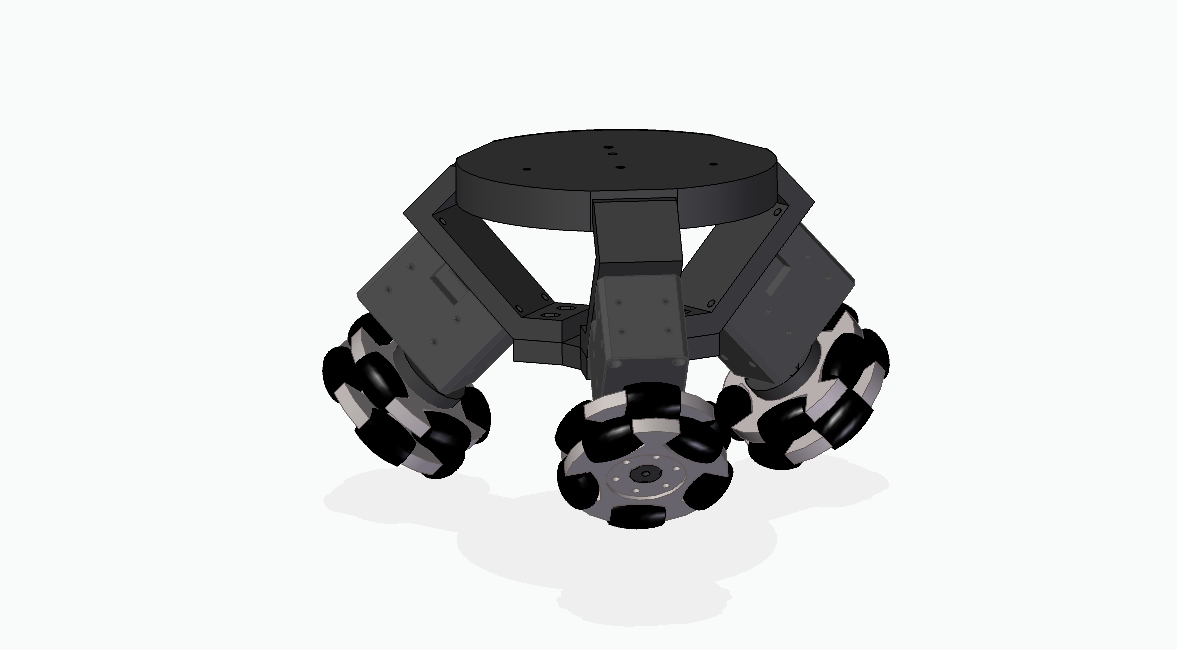
\includegraphics[scale=6.4]{Bilder/Michael/Unterbau.jpg} }
	\caption{Unterbau}
	\label{fig:Unterbau}
\end{figure}

Die Aufgabe des Unterbaus besteht in der Positionierung der Antriebe. Dabei sollte dieser m�glichst leicht und zugleich stabil konstruiert werden. 

Damit das Drehmoment der Motoren optimal auf den Ball �bertragen werden kann, m�ssen die R�der gegen�ber der z-Achse\footnote{Die z-Achse ist die zum Ballbot vertikale Achse.} des Ballbots einen Winkel von $\alpha=45^{\circ}$ einschlie�en. Weiterhin wurden die R�der um einen Winkel von $\beta=120^{\circ}$ zueinander versetzt befestigt. Diese konstruktionsbedingten Winkel sind in Abbildung \ref{fig:konstruktions�bersicht} dargestellt.

\begin{figure}[H]%
	\centering
	{ \scalebox{1}{{\chapter{Konstruktion} \label{ch:konstruktion}

\section{Konzeptionierung} \label{sec:konzeptionierung}

\begin{figure}[H]%
	\centering
	{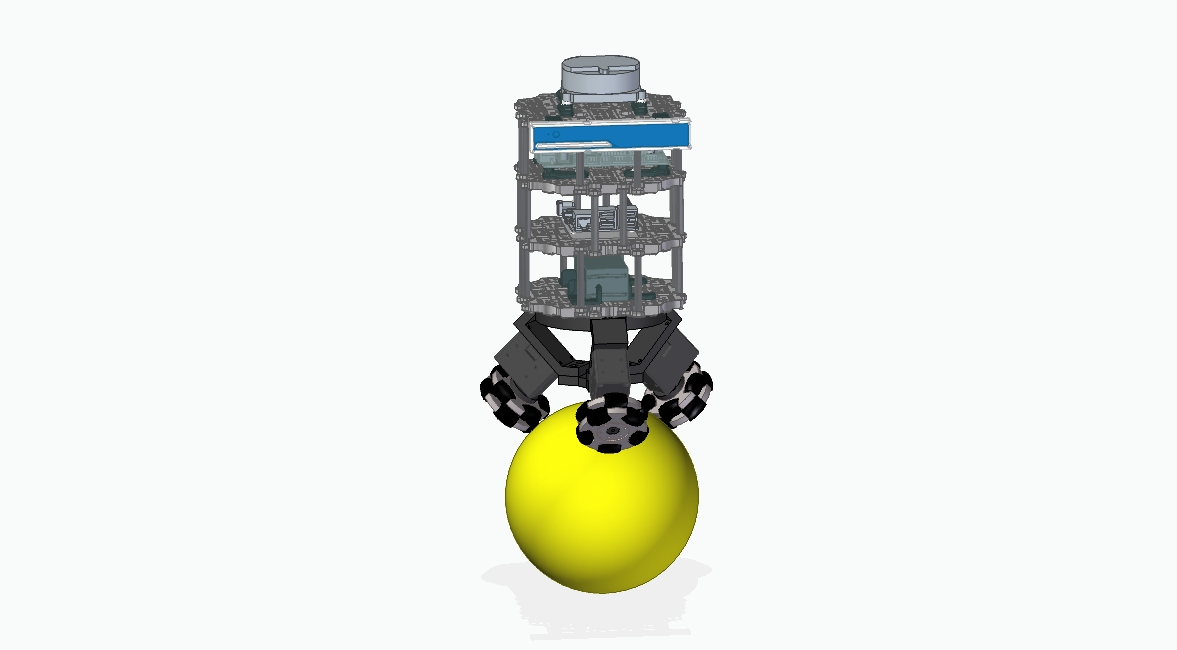
\includegraphics[scale=6.4]{Bilder/Michael/TUD_Ballbot_V30_MS_mit_Raeder_BAll.jpg} }
	\caption{Oberbau, bestehend aus vier Etagen}
	\label{fig:oberbau}
\end{figure}

F�r den Entwurf eines auf einem Ball balancierenden Roboters kann das System zur Vereinfachung als ein inverses Pendel betrachtet werden, dessen Drehachse auf einer beweglichen Plattform gelagert ist. Dies ist in Abbildung \ref{fig:invPendulum} beispielhaft dargestellt. Unter dieser Annahme k�nnen erste Absch�tzungen �ber das dynamische Verhalten getroffen werden. Aus der Anschauung heraus kann direkt gefolgert werden, dass der Pendelarm mit der L�nge $l$ einen Einfluss auf die Pendeldynamik des Systems haben muss. Leitet man nun wie in \cite{pendel}, unter Verwendung der Momentenbilanz das nichtlineare Differenzialgleichungssstem zweiter Ordnung des Auslenkwinkels $\vartheta$ sowie der Schlittenstrecke $x_w$ her, so erh�lt man die Gleichungen: 

        \begin{align} \label{eq:InvPendelThetaDotDot}
            \ddot{\vartheta} &= \frac{l\cdot m}{I}\cdot [-\cos{\vartheta} \cdot \ddot{x}_{w}+g\cdot  \sin{\vartheta}] ,\\   
            \label{eq:InvPendelXDotDot}
            \ddot{x}_w &= \frac{F_{motor}-F_{Reib}}{M+m} + \frac{m\cdot l}{M+m}\dot{\vartheta}^2 \cdot \sin{\vartheta} - \ddot{\vartheta}\cdot cos(\vartheta) . 
        \end{align}


Setzt man nun das Massentr�gheitsmoment des inversen Pendels

        \begin{align} \label{eq:tr�gheitsmoment}
            I &= \frac{4}{3}m\cdot l^2 ,   
        \end{align}
in Gl.\,\ref{eq:InvPendelThetaDotDot} ein, so ergibt sich:  

        \begin{align} \label{eq:InvPendelThetaDotDot_Neu}
            \ddot{\vartheta} &= \frac{3}{4\cdot l}\cdot[-\cos{\vartheta} \cdot \ddot{x}_w+g \cdot  \sin{\vartheta}] . 
        \end{align}

\begin{figure}[H]%
	\centering
	{ \scalebox{1}{{\input{./Bilder/Michael/Schlitten.pdf_tex}}}}%
	\caption{Darstellung eines Ballbots als inverses Pendel}%
	\label{fig:invPendulum}%
\end{figure}%\newline

Anhand der Gleichung (\ref{eq:InvPendelThetaDotDot_Neu}) l�sst sich wie bereits vermutet eine Abh"angikeit der Winkelbeschleunigung $\ddot{\vartheta}$ von der Hebelarml"ange $l$ erkennen. Da sich die Hebelarml�nge jedoch aus der Distanz zwischen Drehachse und Massenschwerpunkt zusammensetzt, bestimmt die Verteilung der Ballbotmasse die Hebelarml�nge des inversen Pendels. Durch das Vergr��ern der Hebelarml�nge $l$ kann so die Winkelbeschleunigung $\ddot{\vartheta}$ f�r kleine Winkelauslenkungen $\Delta \vartheta$ verringert werden. Dadurch ist das System leichter zu stabilisieren. Bei Betrachtung der Gleichung (\ref{eq:InvPendelXDotDot}) l�sst sich jedoch erkennen, dass mit einer Verl�ngerung des Hebelarms $l$ eine gr��ere Beschleunigung $\ddot{x}_w$  des Schlittens einhergehen muss, die durch entsprechend starke Drehmomente realisiert werden kann.

Wendet man dieses Prinzip eines gro�en Hebelarms auf den Ballbot an, so stellt sich jedoch heraus, dass es nur bedingt anwendbar ist. Ursache hierf�r ist die Schnittstelle zwischen omnidirektionalen R�dern und Ball, da hier aufgrund des Reibkoeffizienten nur ein begrenztes Drehmoment �bertragen werden kann. Der Reibkoeffizient begrenzt somit die gew�nschte Sollbeschleunigung des Balles. 

Da eine optimale Auslegung der Pendelarml�nge rechnerisch nur schwer zu bestimmen ist, w�re es w�nschenswert, die Hebelarml�nge durch eine flexible Hardware ver�ndern zu k�nnen. Durch das Hinzuf�gen bzw. Entfernen von weiteren Ebenen im Aufbau des Ballbots kann der Massenschwerpunkt und somit die Pendelarml�nge des Ballbots variabel eingestellt werden. So kann die optimale Konfiguration sehr einfach experimentell bestimmt werden. 

Als Hardware f�r den Ballbot hat man sich daher f�r das TurtleBot3-Paket in der Burger-Variante entschieden. Auf diese soll im Kapitel \ref{sec:Hardware} tiefer eingegangen werden. Bei der Wahl des Balles sowie der Antriebsanordnung hat man sich die Konzepte bereits funktionierender Ballbots als Grundlage hergenommen. Die folgenden Kapitel gehen dabei n�her auf die einzelnen Konstruktionsschritte ein. 

\section{Verwendete Hardware} \label{sec:Hardware}
 Beim Entwurf des Ballbots wurde, wie bereits erw�hnt, auf die leistungsf"ahige Hardware eines TurtleBot3 in der \glqq Burger\grqq-Variante zur"uck gegriffen. Dieses Paket umfasst neben einem robusten mechanischen Aufbau auch alle grundlegenden elektronischen Komponenten wie Sensoren, Mikrocontrollern und Antriebseinheiten, die f�r die Entwicklung eines auf einem Ball balancierenden Roboters ben�tigt werden. Die wichtigsten Komponenten werden in den nachfolgenden Unterkapitel n�her erl�utert.

\subsection{OpenCR-Board} \label{sec:openCr}

Das im Projekt verwendete OpenCR-Board (in der Version 1.0), wie in Abbildung \ref{fig:opencr_board} dargestellt, ist ein Mikrocontroller, der f�r Roboterprojekte in der Gr��e des TurtleBot3-Pakets perfekt geeignet ist. Das gesamte Board, von der Hardware bis zur Software, ist durch Open-Source-Lizenzen frei verf�gbar. Es bietet mit insgesamt 10 verschiedenen Kommunikationsstellen und einer integrierten inertialen Messeinheit (IMU)\footnote{Die verwendete IMU ist die MPU-9250 siehe \url{https://www.invensense.com/products/motion-tracking/9-axis/mpu-9250/}.} bei der Entwicklung von Robotersystemen. Dar�ber hinaus ist das OpenCR-Board mit einem leistungsstarken ARM Cortex-M7 Prozessor ausgestattet.

\begin{figure}[H]%H !htbp
	\centering
	{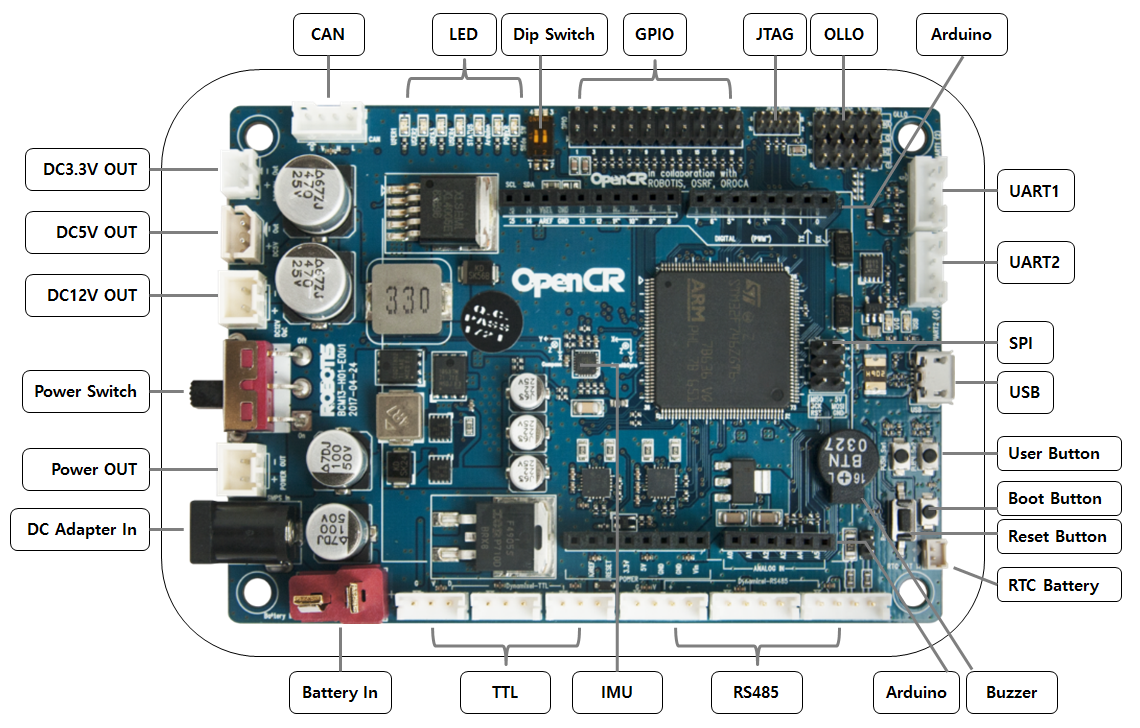
\includegraphics[scale=0.45]{Bilder/Michael/opencr.png} }
	\caption{�bersicht der Schnittstellen des OpenCR-Boards \cite{openCR}}
	\label{fig:opencr_board}
\end{figure}

%https://github.com/ROBOTIS-GIT/emanual/blob/master/docs/en/platform/turtlebot3/appendix_opencr1_0.md

\subsection{Sensorik} \label{sec:sensoren}
Am Ballbot wurden mehrere Sensoren verbaut, die f�r verschiedene Aufgabenbereiche ben�tigt werden. Tabelle \ref{tab:sensoren} zeigt dabei eine �bersicht der Sensoren, die zur Stabilisierung bzw. zur Lokalisation verwendet werden.  


\begin{table}[H]
	\caption["Ubersicht Sensoren]{Sensoren, die im Ballbot verbaut wurden} \label{tab:sensoren}
  		\begin{center}				
		\begin{longtable}{|c||c|c|c|}
		\hline 
  		\multicolumn{4}{|c|}{�bersicht Sensoren} \\ 
  		\hline
  		Kategorie & Stabilisierung & \multicolumn{2}{c|}{Lokalisierung/Interaktion} \\ 
  		\hline
  		\hline
  		Bezeichnung & IMU & Kamera & Laser Distance Sensor\\
  		& MPU-9250 & Intel Realsense R200 & LDS-01\\
  		\hline	\hline
  		
  		 & & & \\
         Taktfrequenz: & 4Hz - 8kHz & 2.5GHz & 1,8 kHz\\
         & & & \\
         Features: & Gyroskop & IR Laser Projector System & DA: 120mm - 3500mm\\
                  & Accelerometer & Full HD RGB Color Stream & Scan Rate: 300$\pm$10 rpm\\
                  & Magnetometer & Onboard Imaging ASIC & Angular Resolution: $1^{\circ}$\\	
  		\hline
		\end{longtable}
  		\end{center}
\end{table} 


\subsection{Motoren} \label{sec:Motoren}

\begin{figure}[H]%
	\centering
	{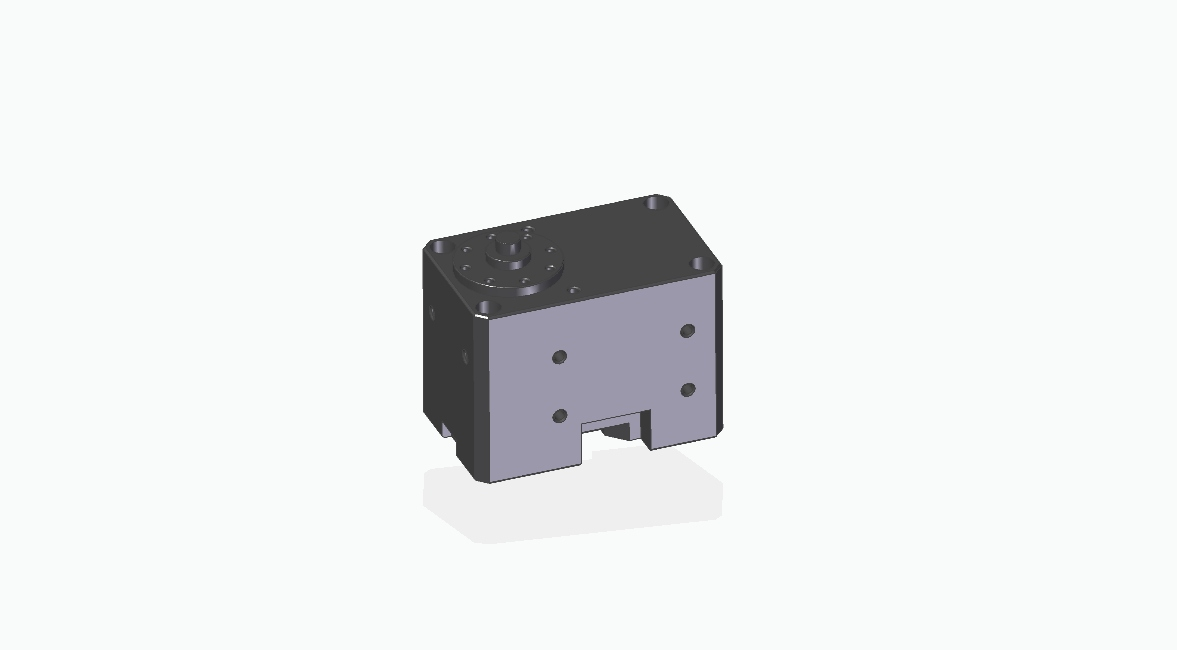
\includegraphics[scale=6.4]{Bilder/Michael/Motoren.jpg} }
	\caption{Motorenspezifikationen}
	\label{fig:motorenspezifikationen}
\end{figure}


Im TurtleBot3-Paket enthalten sind weiterhin auch die Motoren, welche f"ur den Ballbotaufbau verwendet werden. Es handelt sich dabei um Dynamixel Servomotoren der Baureihe XM430-W350-T. Die Motoren haben sich als sehr robust erwiesen und k"onnen durch eine hohe "Ubersetzung von $i=1:353.5$ ein variables ausgangsseitiges Drehmoment von bis zu $3.8$\,Nm bei $11.1$\,V \cite{XM430} erzeugen. Dies ist f"ur die gegebenen Systemkonfiguration mehr als ausreichend. Weiterhin werden von Dynamixel bereits verschiedene Betriebsarten bereitgestellt, in denen die Motoren betrieben werden k"onnen. So bieten die Motoren neben einer Positionsregelung, einer Geschwindigkeitsregelung auch eine Stromregelung. Durch die lineare Abh"angikeit zwischen Drehmoment und Strom kann somit das abtriebseitige Drehmoment geregelt werden.
 
Vom OpenCR-Board werden mittels dem RS485-Protokoll sogennante Units �bertragen. Die Units werden dann intern im Motor in einen realen Sollstrom umgewandelt. Der Strom kann �ber die Formel 

\begin{align} \label{eq:CurrentUnit}
I &= k_{unit}\cdot Units, && \text{mit}  & k_{unit} &= 2,69\cdot 10^{-3} \frac{A}{Unit}
\end{align}

berechnet werden. Anschlie�end kann mit Hilfe der Drehmoment(Nm)-Strom(A)-Kennlinie aus dem Datenblatt \cite{XM430} die spezifische Motorkonstante zu $k_{motor} = 1,63$\,Nm/A bestimmt werden.  
  bestimmt.  Dadurch kann das vom Motor erzeugte Drehmoment aus den Units mittels der Formel 
  \begin{align} \label{eq:CurrentTorque}
  M &= k_{motor} \cdot I \\
    &= k_{motor}\cdot k_{unit} \cdot Units
  \end{align}
  berechnet werden. Insgesamt ergibt sich folgender Gesamtumrechnungsfaktor 
    \begin{align} \label{eq:CurrentTorque}
    k &= k_{motor}\cdot k_{unit} = 228\cdot \frac{Nm}{Unit} 
    \end{align}
    
In der technischen Umsetzung hat sich herausgestellt, dass die Motoren zueinander ein unterschiedliches Verhalten aufweisen und somit die Konstante $k$ nicht f�r alle drei Motoren verwendet werden kann. Daher wurde die Konstante $k$ experimentell bestimmt.
Hierzu wird ein Pr�fhebel der L�nge $l_{pruef}$ f�r die Motoren konstruiert, der w�hrend des Betriebs der Motoren auf eine Waage dr�ckt. Die Motoren werden mit einer bestimmten Folge von dimensionslosen Einheiten angesteuert und jeweils das angezeigte Gewicht der Waage $m$ notiert.
Mit der Beziehung
\begin{align} \label{eq:FMG}
F &= m \cdot g \nonumber
\end{align}
eingesetzt in
\begin{align} 
 M &= F \cdot l_{\text{pruef}}
\end{align}
kann das resultierende Drehmoment $M$ berechnet werden und somit die Konstante $k$ f�r jeden einzelnen Motor.

Bei den Messungen wurde festgestellt, dass das von den Motoren erzeugte Drehmoment einen Drift\footnote{Unter einem Drift ist hier gemeint, dass bei konstantem Anlegen von Units (Stromwert) das Drehmoment �ber die Zeit abnimmt.} aufweist. Dieser Drift konnte reduziert werden, in dem man statt einmaligen Drehmomentbefehlen, die Befehle in Form einer Pulsung wiederkehrend an den Motor �bergeben hat. Die neuen $k$-Faktoren sind �ber die Ergebnisse der Messungen, dargestellt in den Abbildungen \ref{fig:Motorkonstante1}, \ref{fig:Motorkonstante2} und \ref{fig:Motorkonstante3}, mittels der Methode der kleinsten Quadrate berechnet worden. Aus diesen Abbildungen ist zu erkennen, dass sich die Drehmoment-Unit-Konstanten f�r die einzelnen baugleichen Motoren unterscheiden. Dieses Verhalten wurde bei der Implementierung in Kapitel \ref{ch:Implementierung} ber�cksichtigt.
\begin{figure}[!htbp]%
	\centering
	{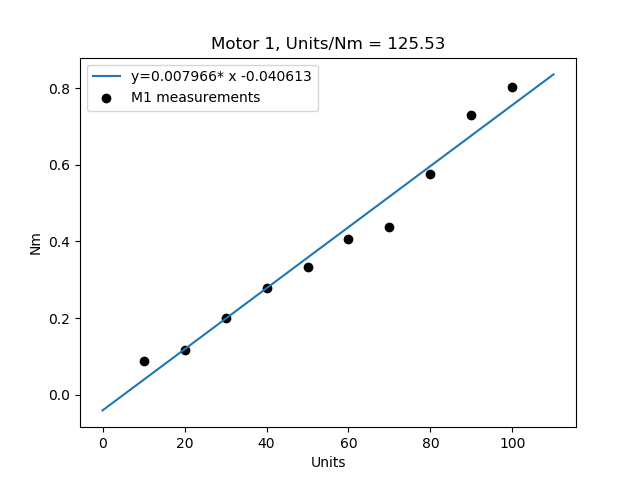
\includegraphics[scale=0.55]{Bilder/Michael/Motor1.png} }
	\caption{Bestimmung der Drehmoment-Unit-Konstante f�r Motor 1}
	\label{fig:Motorkonstante1}
\end{figure}

\begin{figure}[!htbp]%
	\centering
	{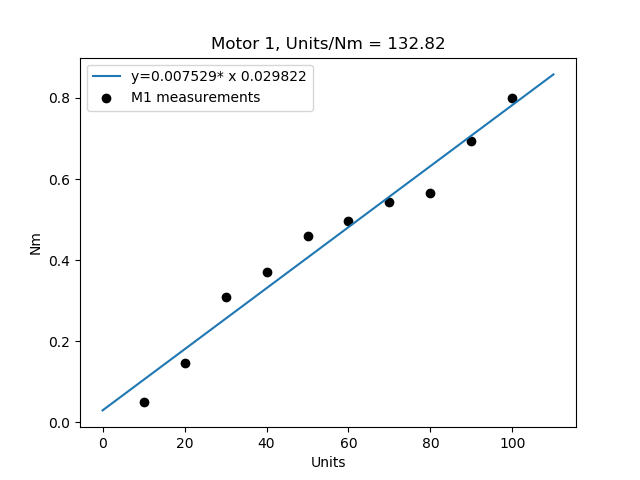
\includegraphics[scale=0.55]{Bilder/Michael/Motor2.png} }
	\caption{Bestimmung der Drehmoment-Unit-Konstante f�r Motor 2}
	\label{fig:Motorkonstante2}
\end{figure}

\begin{figure}[!htbp]%
	\centering
	{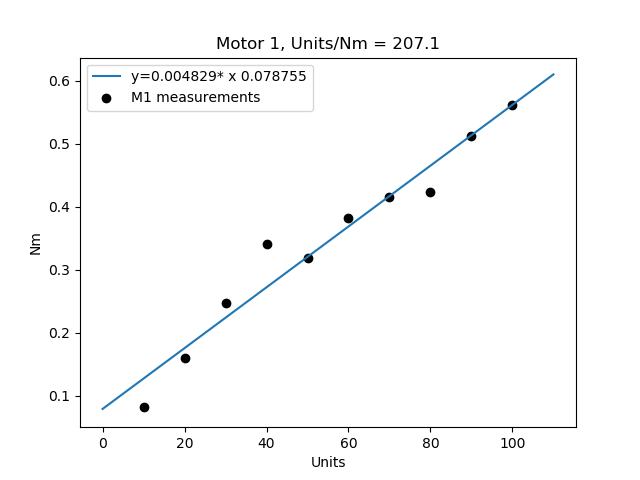
\includegraphics[scale=0.55]{Bilder/Michael/Motor3.png} }
	\caption{Bestimmung der Drehmoment-Unit-Konstante f�r Motor 3}
	\label{fig:Motorkonstante3}
\end{figure}      
            
\section{Ballbot-Design} \label{sec:entwurf}
Die mechanische Systemkonfiguration kann in drei Teile untergliedert werden. Dies ist zum einen der Oberbau (Kap.\ref{sec:oberbau}), der Unterbau (Kap.\ref{sec:unterbau}) sowie der Ball (Kap.\ref{sec:ball}), auf dem das Gesamtsystem bestehend aus Ober- und Unterbau balancieren wird. Nachfolgende Kapitel dokumentieren die Entwicklungsprozesse der einzelnen Teile. 

\subsection{Oberbau} \label{sec:oberbau}

\begin{figure}[H]%
	\centering
	{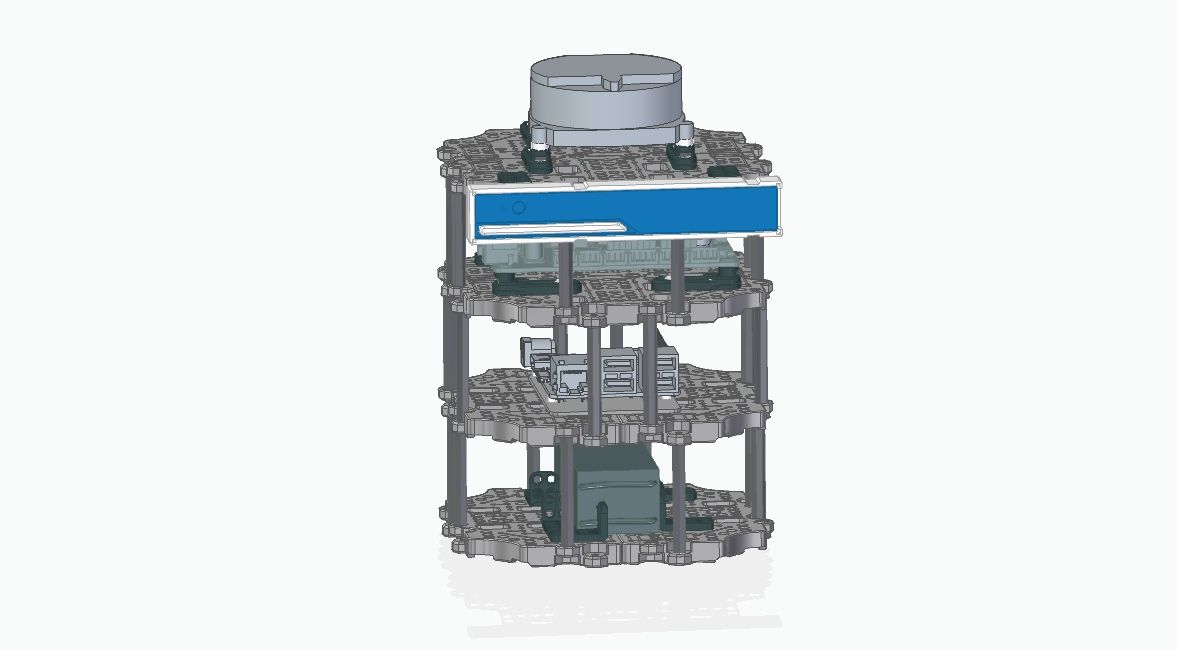
\includegraphics[scale=6.4]{Bilder/Michael/Oberbau.jpg} }
	\caption{Oberbau, bestehend aus vier Etagen}
	\label{fig:oberbau}
\end{figure}

Die Konfiguration des Oberbaus hat sich experimentell unter Ber�cksichtigung der in Kapitel \ref{ch:Modellierung} hergeleiteten Beziehungen ergeben. In der untersten Ebene ist die Batterie platziert. Dar�ber folgt eine Ebene mit einem Up-Level Computer, der f�r rechenintensiver Aufgaben wie der Lokalisation ben�tigt wird. Dieser wird jedoch in dieser Arbeit nicht weiter ber�cksichtigt. Anschlie�end folgt das OpenCR-Board mit den dar�ber platzierten Sensoren zur Lokalisierung des Roboters im Raum, vgl. Abbildung \ref{fig:oberbau}. 


\subsection{Unterbau} \label{sec:unterbau}

\begin{figure}[htb!]%
	\centering
	{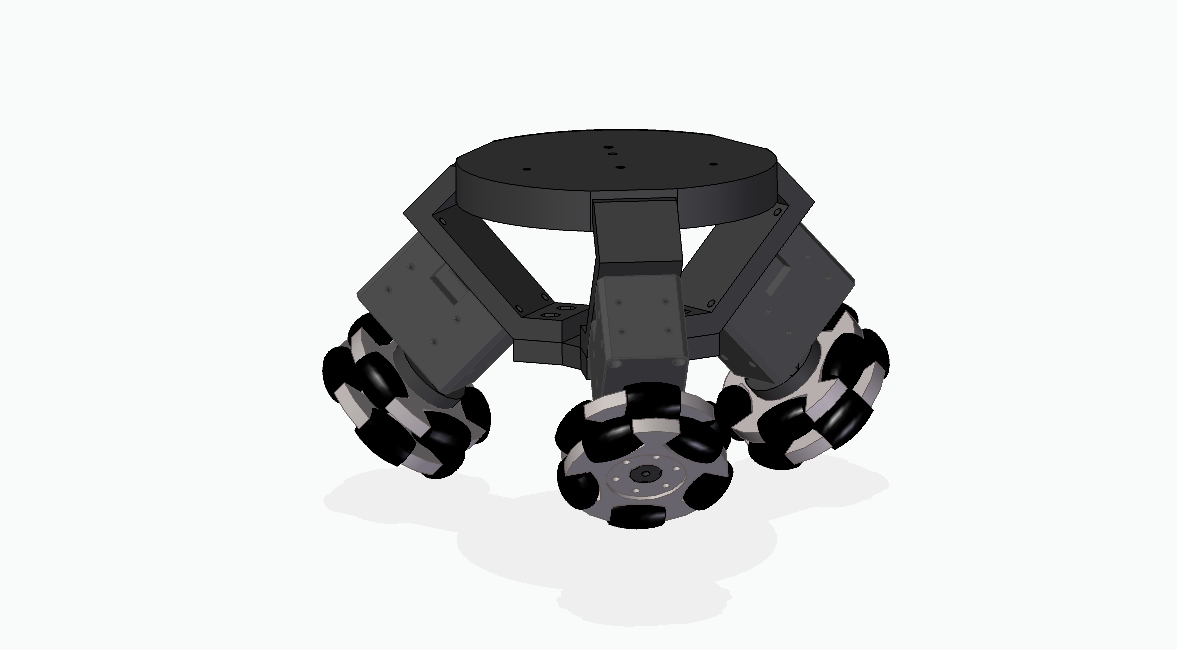
\includegraphics[scale=6.4]{Bilder/Michael/Unterbau.jpg} }
	\caption{Unterbau}
	\label{fig:Unterbau}
\end{figure}

Die Aufgabe des Unterbaus besteht in der Positionierung der Antriebe. Dabei sollte dieser m�glichst leicht und zugleich stabil konstruiert werden. 

Damit das Drehmoment der Motoren optimal auf den Ball �bertragen werden kann, m�ssen die R�der gegen�ber der z-Achse\footnote{Die z-Achse ist die zum Ballbot vertikale Achse.} des Ballbots einen Winkel von $\alpha=45^{\circ}$ einschlie�en. Weiterhin wurden die R�der um einen Winkel von $\beta=120^{\circ}$ zueinander versetzt befestigt. Diese konstruktionsbedingten Winkel sind in Abbildung \ref{fig:konstruktions�bersicht} dargestellt.

\begin{figure}[H]%
	\centering
	{ \scalebox{1}{{\input{./Bilder/Michael/Konstruktion.pdf_tex}}}}%
	\caption{Links: Seitenansicht der Ball-Rad- Konfiguration. \\Rechts: Draufsicht der Ball-Rad -Konfiguration  }%
	\label{fig:konstruktions�bersicht}
\end{figure}%\newline

Unter Ber�cksichtigung dieser Vorgaben ist der Unterbau entwickelt worden. Die daf�r notwendigen Konstruktionen sind mit dem CAD-Tool SolidEdge durchgef�hrt und anschlie�end auf einen 3D-Drucker �bertragen und gedruckt worden. Auf diesem Weg war es m�glich schnell und kosteng�nstig neue Ideen und Designs umzusetzen. Diese Schritte werden im Kapitel \ref{sec:SolidEdge} erl�utert. Zun�chst soll jedoch noch auf die Wahl des Balls eingegangen werden. 

\subsection{Wahl des Balls} \label{sec:ball}
Der Ball stellt eine weitere Schl�sselkomponente bei der Entwicklung eines Ballbots dar. Im Verlauf der Balancierungstest sind einige verschiede B�lle zum Einsatz gekommen. Die Suche nach einem optimalen Ball hat sich dabei als �u�erst schwierig herausgestellt, da mehrere Parameter des Balls Einfluss auf das Balancierverhalten haben. Neben der Gr��e und Kompressibilit�t spielen besonders auch der Reibkoeffizient und das Tr�gheitsmoment eine gro�e Rolle. 

Die Gr��e des Balles muss auf die Auslegung des Unterbaus ausgerichtet werden, da sich sonst ein falscher Winkel $\alpha$ f�r das reale System ergibt. Weiterhin ist bei vielen B�llen immer wieder Schlupf zwischen Omniwheels und Ball aufgetreten. Sobald Schlupf auftrat, konnte der Ballbot durch die Regelung nicht mehr stabilisiert werden. Dies gilt es daher unbedingt zu vermeiden. Zudem d�rfen keine Verformungen des Balles bei Belastungen durch den Ballbot auftreten, da sich der Ballbot sonst aufschaukelt und das Regelverhalten einer unged�mpften Schwingung gleicht.
Am Ende der Experimente hat sich ein Handball der Gr��e II auf einer d�nnen Schaumstoffmatte als bester Kompromiss herausgestellt. Die Schaumstoffmatte wurde dabei zur D�mpfung der Ballbewegung verwendet.

\section{Konstruktion mittels SolidEdge} \label{sec:SolidEdge}
SolidEdge ist eine Computer gest�tztes Design(CAD)-Software, die ein rechnergest�tztes Konstruieren einzelner Bauteile sowie ganzer Baugruppen eines Produktes, einer Maschine, etc. erm�glicht. Weiterhin gibt es auch Tools zur Bauteil-Optimierung und Simulation von Str�mungen. SolidEdge wird f�r Studenten kostenlos von der Siemens Industry Software GmbH zur Verf�gung gestellt und kann unter Angabe der pers�nlichen Daten heruntergeladen werden\footnote{\url{https://www.plm.automation.siemens.com/plmapp/education/solid-edge/en_us/free-software/student} (Stand: 07.02.2018)}. \\

\subsection{SolidEdge - Eine kurze Einf�hrung} \label{whatIs}
Bei der Konstruktion der einzelnen Unterbaukomponenten des Ballbots sind haupts�chlich zwei Funktionen von SolidEdge genutzt worden. Zum einen die Erzeugung einzelner Bauteile, worunter im Folgenden ein einzelner K�rper\footnote{Unter dem Begriff K�rper soll in diesem Anwendungsfall ein einzelnes, nicht aus mehreren Teilkomponenten bestehendes, Werkst�ck verstanden werden.} verstanden wird, sowie die Erzeugung von Baugruppen \footnote{Zusammensetzung/Montage einzelner K�rper zu einer Gruppe.}. Bei einer Baugruppe werden die Bauteile automatisch je nach Montagevorschrift zusammengef�gt und �ber sogenannte Beziehungen miteinander verbunden. Wird eine Baugruppe in eine neue Datei geladen, verh�lt sich die Baugruppe durch die definierten Beziehungen wie ein einzelner K�rper. Auf diesem Weg k�nnen in eine Baugruppe auch andere Baugruppen geladen und miteinander in Beziehung gestellt werden. Das macht ein schrittweises und �bersichtliches Zusammensetzen der Gesamtkonstruktion m�glich.  

\subsection{SolidEdge - Umsetzung} \label{subsec:Umsetzung}
Es soll nun ein Einblick in die Vorgehensweise bei der Konstruktion des Unterbaus mit SolidEdge gegeben werden. Abbildung \ref{fig:Unterbau} zeigt die Baugruppe \glqq Unterbau\grqq. Folgende Kriterien galt es dabei zu erf�llen: Die Baugruppe sollte aus mehreren K�rpern besteht, sodass ein einfaches Montieren der einzelnen Komponenten m�glich ist. Weiterhin sollte eine flexible Konstruktion entwickelt werden, um den Ballbot auf B�llen mit verschiedenen Radien testen zu k�nnen. Dies wurde durch eine Teleskopsystem erm�glicht, sodass die Motoren inklusive R�der radial nach au�en bzw. innen geschoben werden k�nnen. Dies ist in Abbildung \ref{fig:Motorenhalter} dargestellt. 
\begin{figure}[!htbp]%
	\centering
	{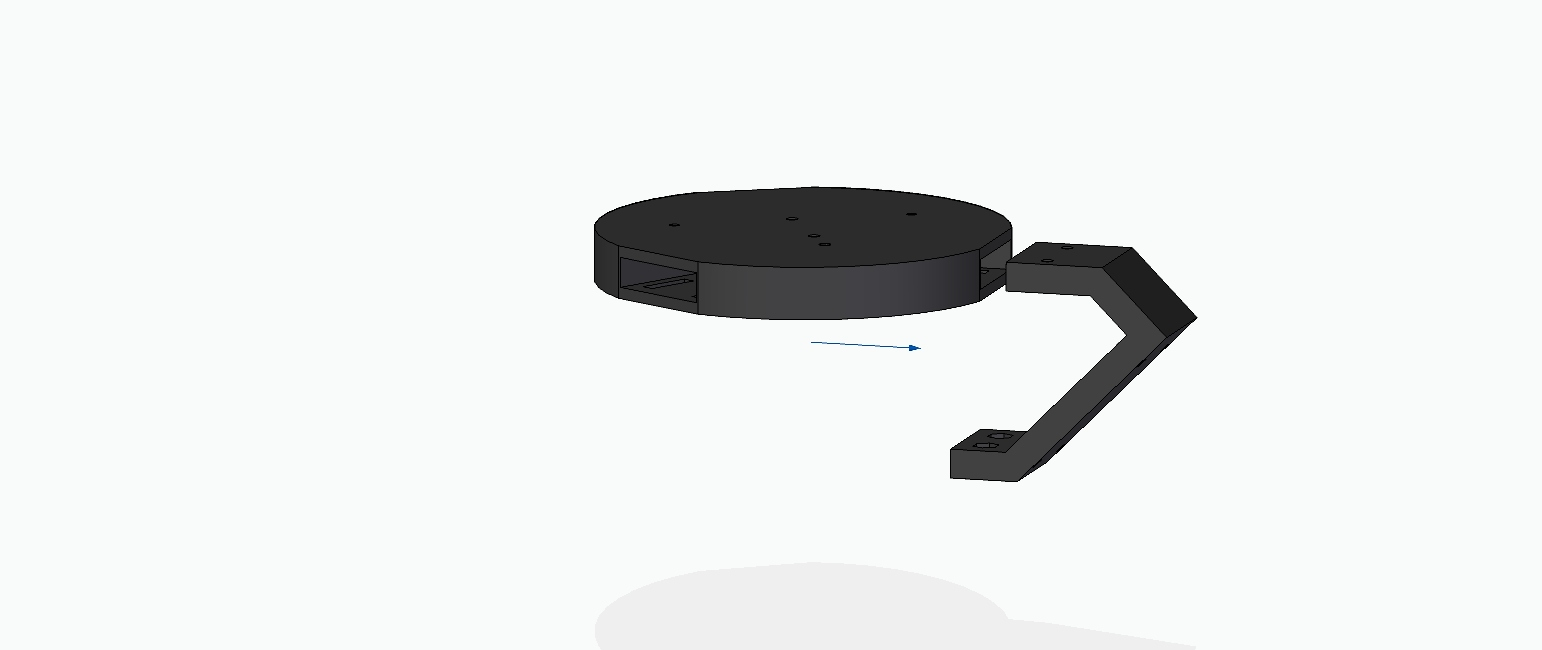
\includegraphics[scale=4.9]{Bilder/Michael/Traeger_Halterung_Explosion.jpg} }
	\caption{Teleskopsystem bestehend aus Tr�gerplatte(links) und Motorenhalter(rechts)}
	\label{fig:Motorenhalter}
\end{figure}

R�cksicht wurde weiterhin auf eine stabile Integration der Motoren in die Gesamtkonstruktion genommen. So soll bei den wirkenden Kr�ften und Momenten, Bewegungen der Unterbaukomponenten relativ zu einander vermieden werden. Integriert wurden die Motoren daher �ber vier M3 Zylinderkopfschrauben an den sogenannten Motorenhaltern, wie in Abbildung \ref{fig:antrieb} dargestellt. Die F�hrungsschiene des Motorenhalters  wird in eine F�hrungsnut der Tr�gerplatte passgenau eingef�hrt und verschraubt.


\begin{figure}[!htbp]%
	\centering
	{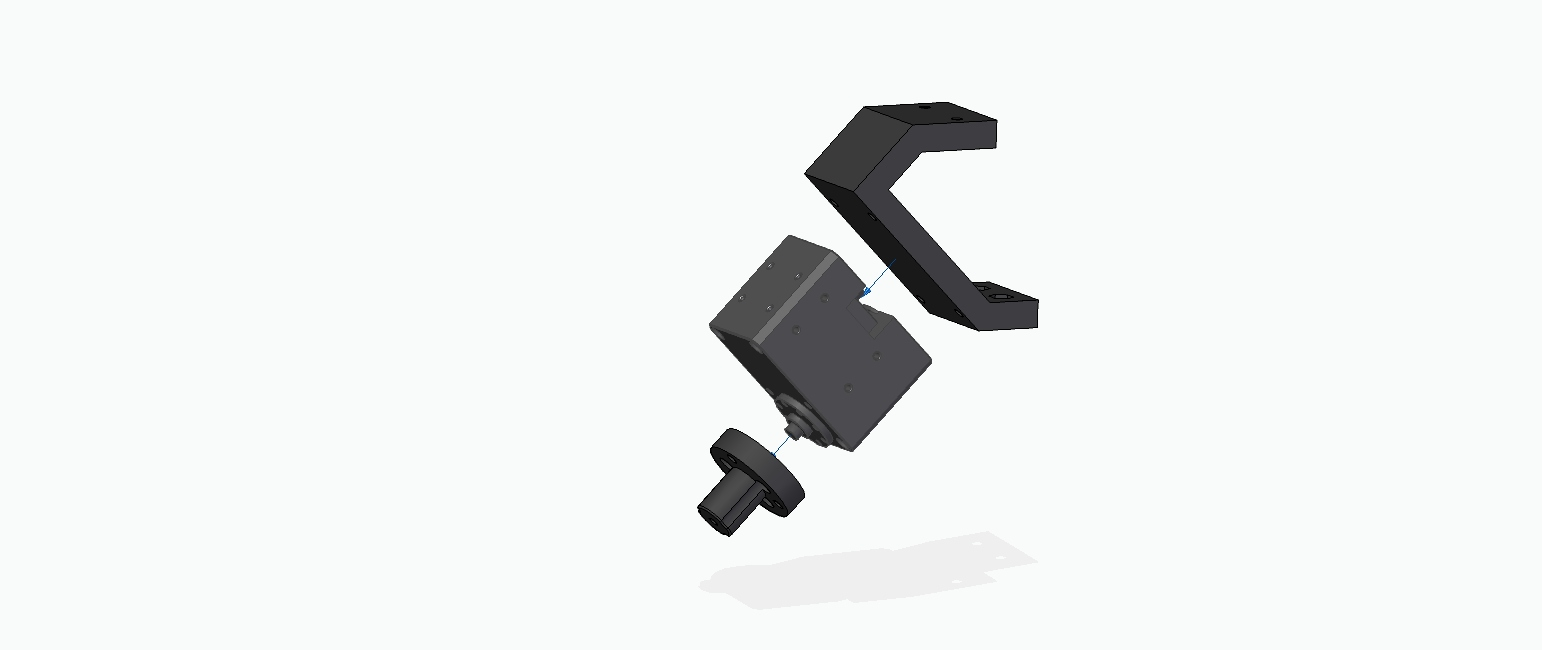
\includegraphics[scale=4.8]{Bilder/Michael/Motor_Mitnehmer_Halterung_Explosion.jpg} }
	\caption{Antriebsvorrichtung bestehend aus Mitnehmer (unten), Motor (mitte) und Motorenhalter (oben). }
	\label{fig:antrieb}
\end{figure}

Um die R�der, dargestellt in Abbildung \ref{fig:wheel} an die Motorwellen zu befestigen, sind spezielle Mitnehmer konstruiert worden, die in Abbildung \ref{fig:antrieb} dargestellt sind.

Wichtige Kriterien, die es hierbei zu erf�llen gab, waren eine spielfrei �bertragung der Momente und Kr�fte sowie eine m�glichst kurze Distanz zwischen den R�dern und den Motoren.

Nach einigen Tests hat sich herausgestellt, dass die gew�nschte Stabilit�t es Unterbaus nicht gegeben war. Die Konstruktion musste also noch verst�rkt werden. Um die n�tige Stabilit�t herzustellen, sind die Motorenhalter um eine Anflanschfl�che erweitert worden. So k�nnen die Motorenhalter �ber ein Y-f�rmiges Verbindungsst�ck, dargestellt in Abbildung \ref{fig:kreisring}, miteinander gekoppelt werden. Hierbei wurde eine flexible Anpassung an unterschiedlichen Ballradien ber�cksichtigt.
\begin{figure}[!htbp]%
	\centering
	{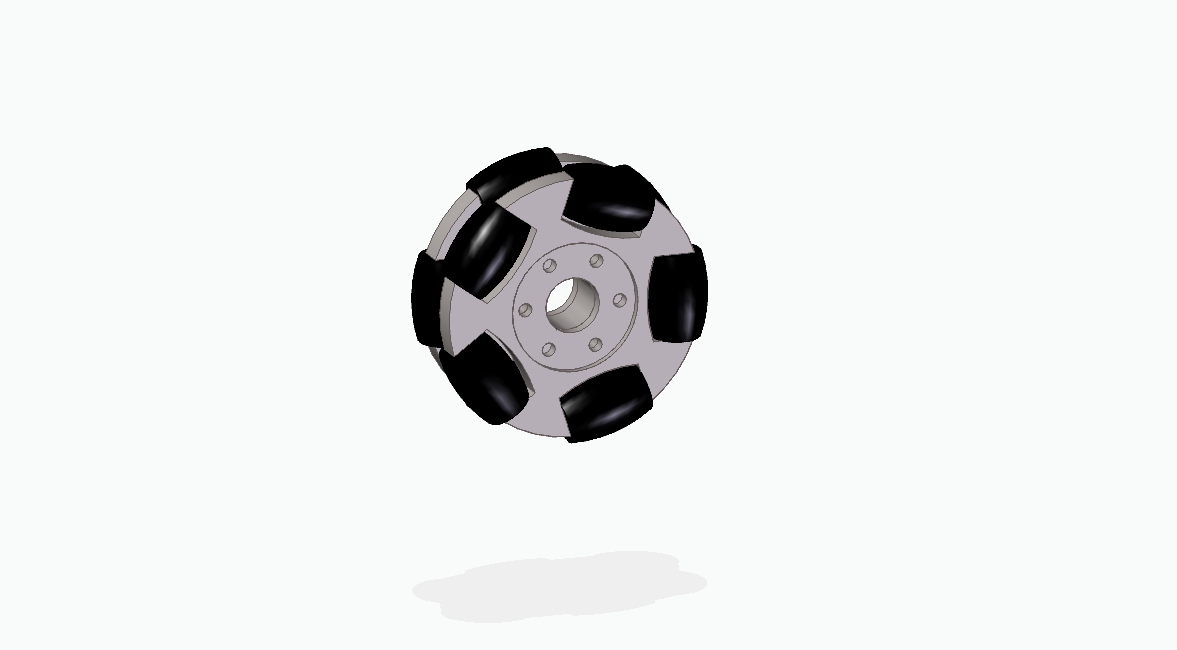
\includegraphics[scale=6.4]{Bilder/Michael/Wheel2_Double.jpg} }
	\caption{Modell eines omnidirektionalen Rades}
	\label{fig:wheel}
\end{figure}

\begin{figure}[!htbp]%
	\centering
	{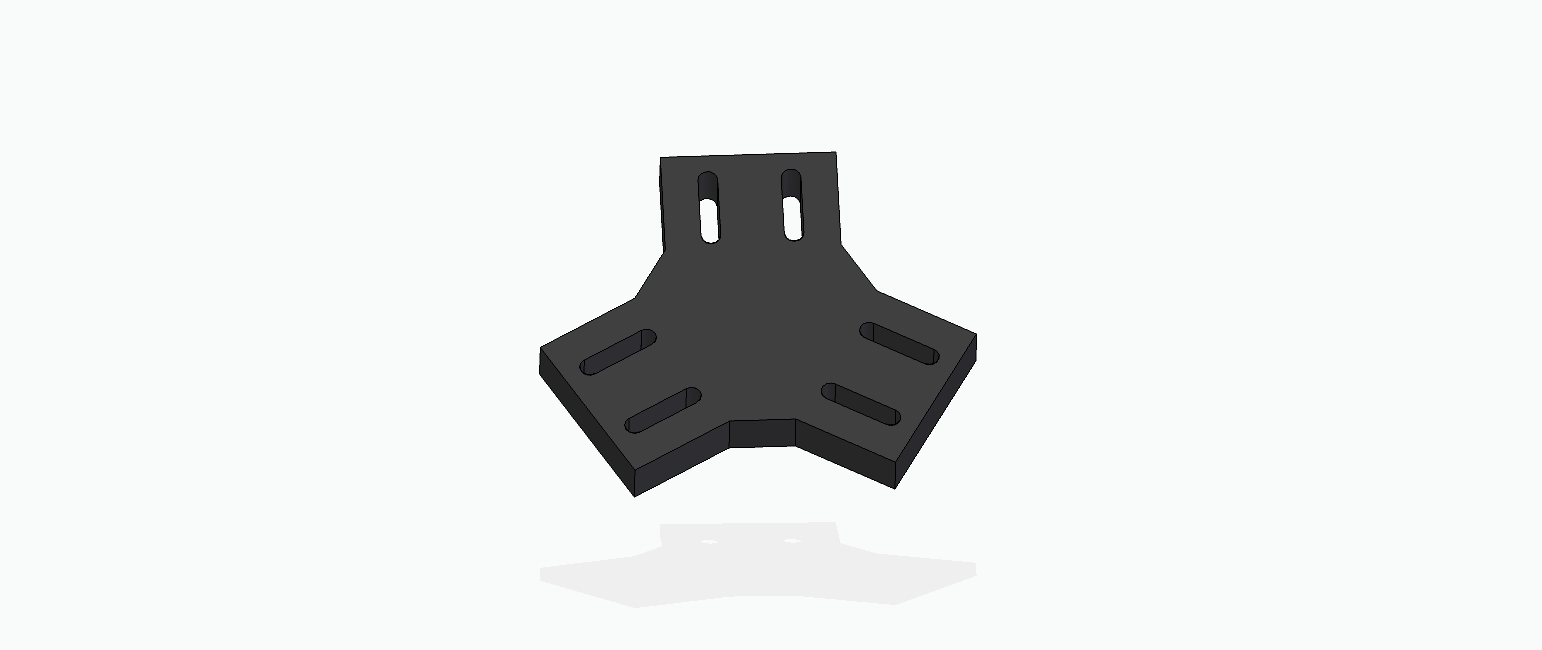
\includegraphics[scale=4.8]{Bilder/Michael/Kreisring_Stabi.jpg} }
	\caption{Y-f�rmiges Verbindungsst�ck des Unterbaus.}
	\label{fig:kreisring}
\end{figure}

\section{Fertigung der Komponenten} \label{sec:Fertigung}
Neben dem Zugang zu einem professionellen CAD-Tool bestand auch Zugang zu einem 3D-Drucker der Firma Oktoprint. Dies erm�glichte eine kosteng�nstige und schnelle Fertigung der konstruierten Bauteile. Verwendete wurde dabei das Filament Polylactide (PLA). PLA ist ein sehr verbreiteter biokompatibler Kunstoff, der eine hohe Oberfl�chenh�rte, hohe Steifigkeit und eine hohe Zugfestigkeit bietet \cite{pla}. 

Der fertige Entwurf wurde schlie�lich als .stl exportiert und in das 3D-Druckprogramm CURA geladen. Mit CURA konnte anschlie�end die F�lldichte, die Qualit�t, Druckgeschwindigkeit und der Einsatz von St�tzhilfen f�r den jeweiligen Druck eingestellt werden. Die gew�nschten Genauigkeiten konnten mittels dieser Fertigungsweise eingehalten werden. So hat der Druck auch an kritischen Stellen wie der Einschubverbindung zwischen Tr�gerplatte und Motorenhalter �berzeugt. Es war nach Einschub und Verschraubung der Motorenhalter mit der Tr�gerplatte kein Spiel vorhanden. }}}%
	\caption{Links: Seitenansicht der Ball-Rad- Konfiguration. \\Rechts: Draufsicht der Ball-Rad -Konfiguration  }%
	\label{fig:konstruktions�bersicht}
\end{figure}%\newline

Unter Ber�cksichtigung dieser Vorgaben ist der Unterbau entwickelt worden. Die daf�r notwendigen Konstruktionen sind mit dem CAD-Tool SolidEdge durchgef�hrt und anschlie�end auf einen 3D-Drucker �bertragen und gedruckt worden. Auf diesem Weg war es m�glich schnell und kosteng�nstig neue Ideen und Designs umzusetzen. Diese Schritte werden im Kapitel \ref{sec:SolidEdge} erl�utert. Zun�chst soll jedoch noch auf die Wahl des Balls eingegangen werden. 

\subsection{Wahl des Balls} \label{sec:ball}
Der Ball stellt eine weitere Schl�sselkomponente bei der Entwicklung eines Ballbots dar. Im Verlauf der Balancierungstest sind einige verschiede B�lle zum Einsatz gekommen. Die Suche nach einem optimalen Ball hat sich dabei als �u�erst schwierig herausgestellt, da mehrere Parameter des Balls Einfluss auf das Balancierverhalten haben. Neben der Gr��e und Kompressibilit�t spielen besonders auch der Reibkoeffizient und das Tr�gheitsmoment eine gro�e Rolle. 

Die Gr��e des Balles muss auf die Auslegung des Unterbaus ausgerichtet werden, da sich sonst ein falscher Winkel $\alpha$ f�r das reale System ergibt. Weiterhin ist bei vielen B�llen immer wieder Schlupf zwischen Omniwheels und Ball aufgetreten. Sobald Schlupf auftrat, konnte der Ballbot durch die Regelung nicht mehr stabilisiert werden. Dies gilt es daher unbedingt zu vermeiden. Zudem d�rfen keine Verformungen des Balles bei Belastungen durch den Ballbot auftreten, da sich der Ballbot sonst aufschaukelt und das Regelverhalten einer unged�mpften Schwingung gleicht.
Am Ende der Experimente hat sich ein Handball der Gr��e II auf einer d�nnen Schaumstoffmatte als bester Kompromiss herausgestellt. Die Schaumstoffmatte wurde dabei zur D�mpfung der Ballbewegung verwendet.

\section{Konstruktion mittels SolidEdge} \label{sec:SolidEdge}
SolidEdge ist eine Computer gest�tztes Design(CAD)-Software, die ein rechnergest�tztes Konstruieren einzelner Bauteile sowie ganzer Baugruppen eines Produktes, einer Maschine, etc. erm�glicht. Weiterhin gibt es auch Tools zur Bauteil-Optimierung und Simulation von Str�mungen. SolidEdge wird f�r Studenten kostenlos von der Siemens Industry Software GmbH zur Verf�gung gestellt und kann unter Angabe der pers�nlichen Daten heruntergeladen werden\footnote{\url{https://www.plm.automation.siemens.com/plmapp/education/solid-edge/en_us/free-software/student} (Stand: 07.02.2018)}. \\

\subsection{SolidEdge - Eine kurze Einf�hrung} \label{whatIs}
Bei der Konstruktion der einzelnen Unterbaukomponenten des Ballbots sind haupts�chlich zwei Funktionen von SolidEdge genutzt worden. Zum einen die Erzeugung einzelner Bauteile, worunter im Folgenden ein einzelner K�rper\footnote{Unter dem Begriff K�rper soll in diesem Anwendungsfall ein einzelnes, nicht aus mehreren Teilkomponenten bestehendes, Werkst�ck verstanden werden.} verstanden wird, sowie die Erzeugung von Baugruppen \footnote{Zusammensetzung/Montage einzelner K�rper zu einer Gruppe.}. Bei einer Baugruppe werden die Bauteile automatisch je nach Montagevorschrift zusammengef�gt und �ber sogenannte Beziehungen miteinander verbunden. Wird eine Baugruppe in eine neue Datei geladen, verh�lt sich die Baugruppe durch die definierten Beziehungen wie ein einzelner K�rper. Auf diesem Weg k�nnen in eine Baugruppe auch andere Baugruppen geladen und miteinander in Beziehung gestellt werden. Das macht ein schrittweises und �bersichtliches Zusammensetzen der Gesamtkonstruktion m�glich.  

\subsection{SolidEdge - Umsetzung} \label{subsec:Umsetzung}
Es soll nun ein Einblick in die Vorgehensweise bei der Konstruktion des Unterbaus mit SolidEdge gegeben werden. Abbildung \ref{fig:Unterbau} zeigt die Baugruppe \glqq Unterbau\grqq. Folgende Kriterien galt es dabei zu erf�llen: Die Baugruppe sollte aus mehreren K�rpern besteht, sodass ein einfaches Montieren der einzelnen Komponenten m�glich ist. Weiterhin sollte eine flexible Konstruktion entwickelt werden, um den Ballbot auf B�llen mit verschiedenen Radien testen zu k�nnen. Dies wurde durch eine Teleskopsystem erm�glicht, sodass die Motoren inklusive R�der radial nach au�en bzw. innen geschoben werden k�nnen. Dies ist in Abbildung \ref{fig:Motorenhalter} dargestellt. 
\begin{figure}[!htbp]%
	\centering
	{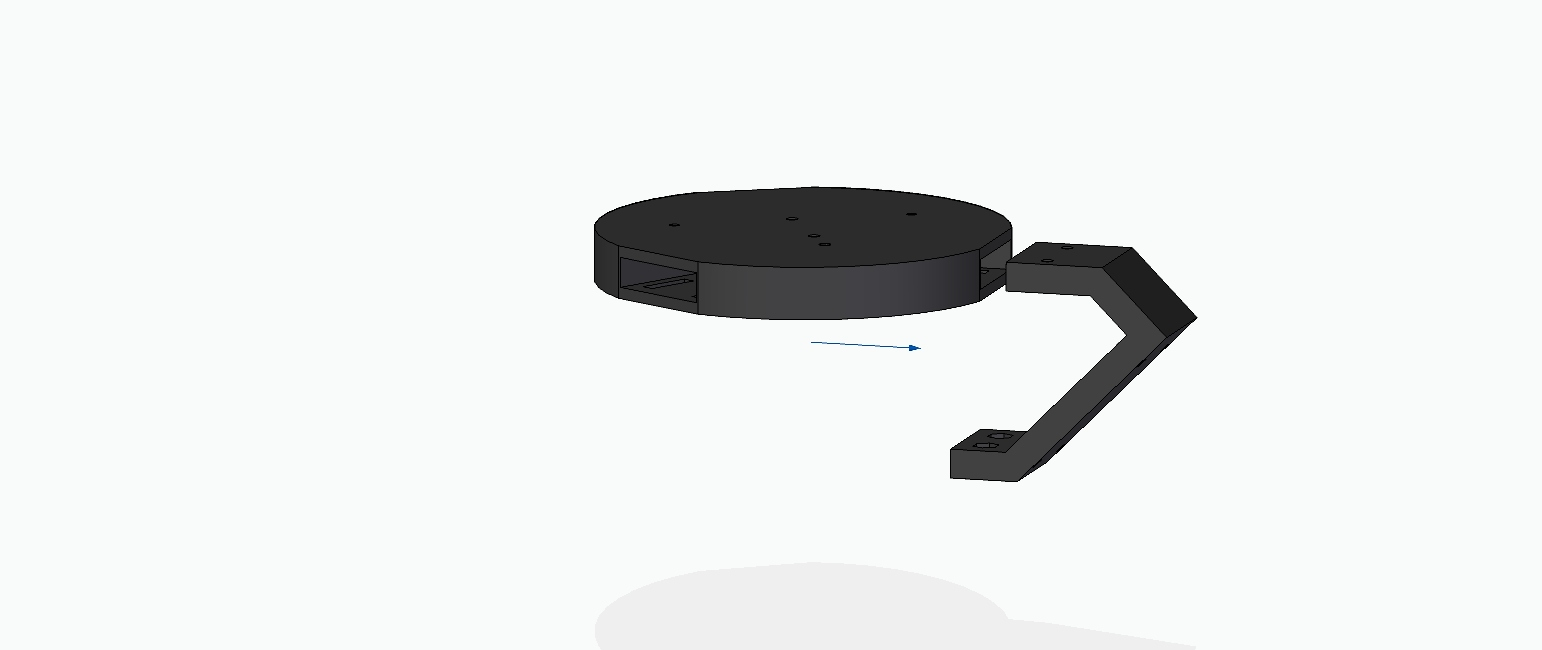
\includegraphics[scale=4.9]{Bilder/Michael/Traeger_Halterung_Explosion.jpg} }
	\caption{Teleskopsystem bestehend aus Tr�gerplatte(links) und Motorenhalter(rechts)}
	\label{fig:Motorenhalter}
\end{figure}

R�cksicht wurde weiterhin auf eine stabile Integration der Motoren in die Gesamtkonstruktion genommen. So soll bei den wirkenden Kr�ften und Momenten, Bewegungen der Unterbaukomponenten relativ zu einander vermieden werden. Integriert wurden die Motoren daher �ber vier M3 Zylinderkopfschrauben an den sogenannten Motorenhaltern, wie in Abbildung \ref{fig:antrieb} dargestellt. Die F�hrungsschiene des Motorenhalters  wird in eine F�hrungsnut der Tr�gerplatte passgenau eingef�hrt und verschraubt.


\begin{figure}[!htbp]%
	\centering
	{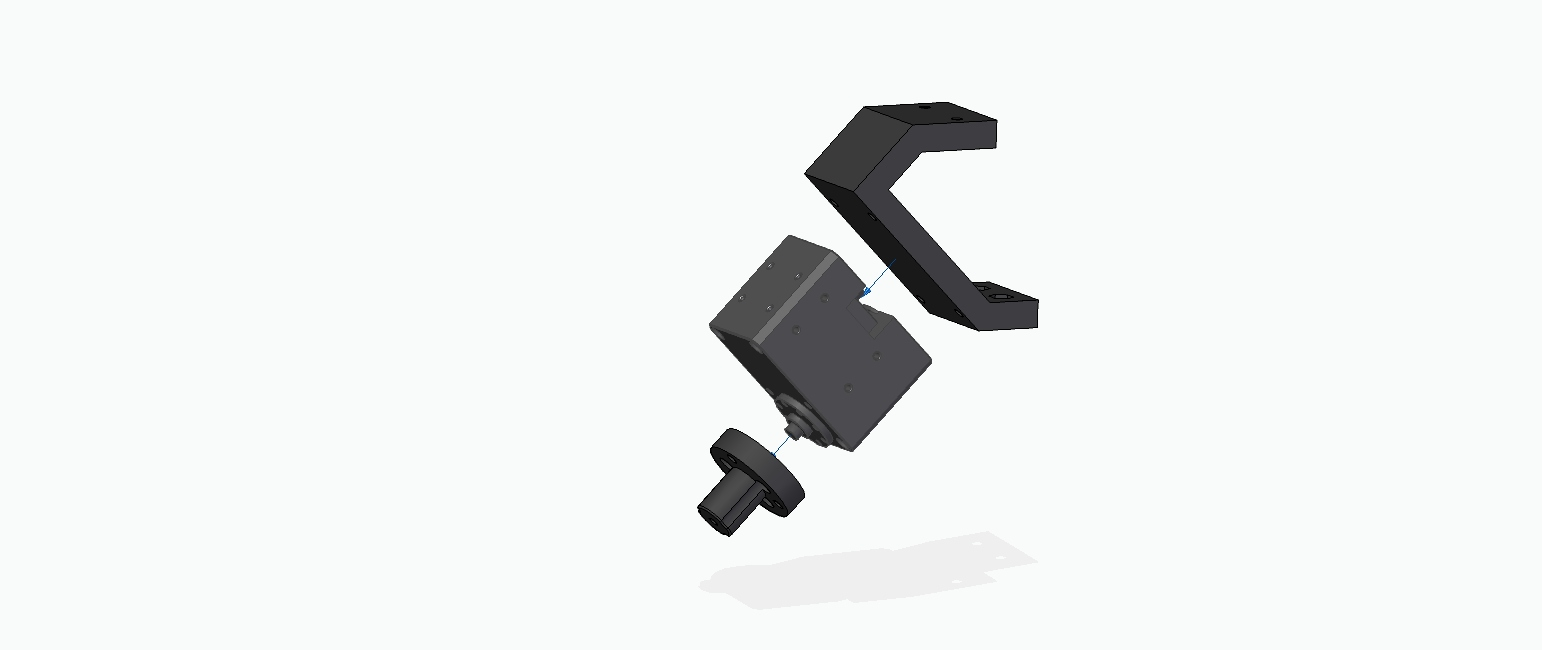
\includegraphics[scale=4.8]{Bilder/Michael/Motor_Mitnehmer_Halterung_Explosion.jpg} }
	\caption{Antriebsvorrichtung bestehend aus Mitnehmer (unten), Motor (mitte) und Motorenhalter (oben). }
	\label{fig:antrieb}
\end{figure}

Um die R�der, dargestellt in Abbildung \ref{fig:wheel} an die Motorwellen zu befestigen, sind spezielle Mitnehmer konstruiert worden, die in Abbildung \ref{fig:antrieb} dargestellt sind.

Wichtige Kriterien, die es hierbei zu erf�llen gab, waren eine spielfrei �bertragung der Momente und Kr�fte sowie eine m�glichst kurze Distanz zwischen den R�dern und den Motoren.

Nach einigen Tests hat sich herausgestellt, dass die gew�nschte Stabilit�t es Unterbaus nicht gegeben war. Die Konstruktion musste also noch verst�rkt werden. Um die n�tige Stabilit�t herzustellen, sind die Motorenhalter um eine Anflanschfl�che erweitert worden. So k�nnen die Motorenhalter �ber ein Y-f�rmiges Verbindungsst�ck, dargestellt in Abbildung \ref{fig:kreisring}, miteinander gekoppelt werden. Hierbei wurde eine flexible Anpassung an unterschiedlichen Ballradien ber�cksichtigt.
\begin{figure}[!htbp]%
	\centering
	{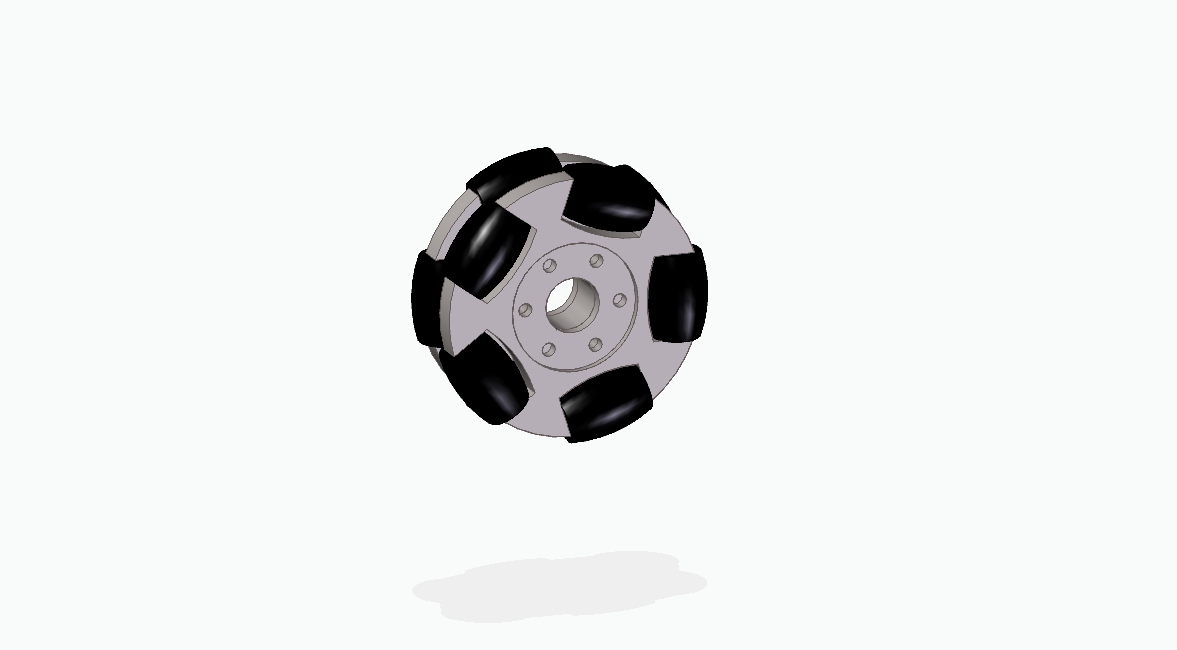
\includegraphics[scale=6.4]{Bilder/Michael/Wheel2_Double.jpg} }
	\caption{Modell eines omnidirektionalen Rades}
	\label{fig:wheel}
\end{figure}

\begin{figure}[!htbp]%
	\centering
	{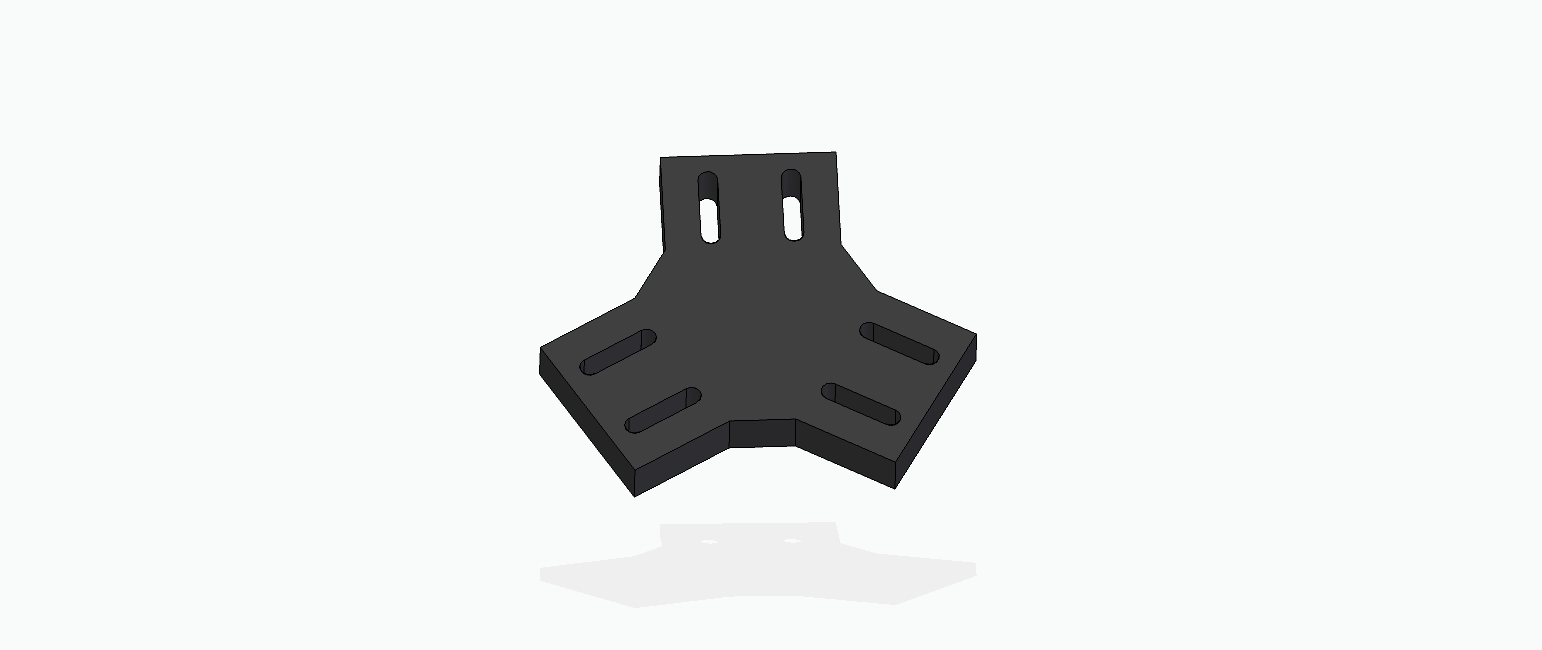
\includegraphics[scale=4.8]{Bilder/Michael/Kreisring_Stabi.jpg} }
	\caption{Y-f�rmiges Verbindungsst�ck des Unterbaus.}
	\label{fig:kreisring}
\end{figure}

\section{Fertigung der Komponenten} \label{sec:Fertigung}
Neben dem Zugang zu einem professionellen CAD-Tool bestand auch Zugang zu einem 3D-Drucker der Firma Oktoprint. Dies erm�glichte eine kosteng�nstige und schnelle Fertigung der konstruierten Bauteile. Verwendete wurde dabei das Filament Polylactide (PLA). PLA ist ein sehr verbreiteter biokompatibler Kunstoff, der eine hohe Oberfl�chenh�rte, hohe Steifigkeit und eine hohe Zugfestigkeit bietet \cite{pla}. 

Der fertige Entwurf wurde schlie�lich als .stl exportiert und in das 3D-Druckprogramm CURA geladen. Mit CURA konnte anschlie�end die F�lldichte, die Qualit�t, Druckgeschwindigkeit und der Einsatz von St�tzhilfen f�r den jeweiligen Druck eingestellt werden. Die gew�nschten Genauigkeiten konnten mittels dieser Fertigungsweise eingehalten werden. So hat der Druck auch an kritischen Stellen wie der Einschubverbindung zwischen Tr�gerplatte und Motorenhalter �berzeugt. Es war nach Einschub und Verschraubung der Motorenhalter mit der Tr�gerplatte kein Spiel vorhanden. }}}%
	\caption{Links: Seitenansicht der Ball-Rad- Konfiguration. \\Rechts: Draufsicht der Ball-Rad -Konfiguration  }%
	\label{fig:konstruktions�bersicht}
\end{figure}%\newline

Unter Ber�cksichtigung dieser Vorgaben ist der Unterbau entwickelt worden. Die daf�r notwendigen Konstruktionen sind mit dem CAD-Tool SolidEdge durchgef�hrt und anschlie�end auf einen 3D-Drucker �bertragen und gedruckt worden. Auf diesem Weg war es m�glich schnell und kosteng�nstig neue Ideen und Designs umzusetzen. Diese Schritte werden im Kapitel \ref{sec:SolidEdge} erl�utert. Zun�chst soll jedoch noch auf die Wahl des Balls eingegangen werden. 

\subsection{Wahl des Balls} \label{sec:ball}
Der Ball stellt eine weitere Schl�sselkomponente bei der Entwicklung eines Ballbots dar. Im Verlauf der Balancierungstest sind einige verschiede B�lle zum Einsatz gekommen. Die Suche nach einem optimalen Ball hat sich dabei als �u�erst schwierig herausgestellt, da mehrere Parameter des Balls Einfluss auf das Balancierverhalten haben. Neben der Gr��e und Kompressibilit�t spielen besonders auch der Reibkoeffizient und das Tr�gheitsmoment eine gro�e Rolle. 

Die Gr��e des Balles muss auf die Auslegung des Unterbaus ausgerichtet werden, da sich sonst ein falscher Winkel $\alpha$ f�r das reale System ergibt. Weiterhin ist bei vielen B�llen immer wieder Schlupf zwischen Omniwheels und Ball aufgetreten. Sobald Schlupf auftrat, konnte der Ballbot durch die Regelung nicht mehr stabilisiert werden. Dies gilt es daher unbedingt zu vermeiden. Zudem d�rfen keine Verformungen des Balles bei Belastungen durch den Ballbot auftreten, da sich der Ballbot sonst aufschaukelt und das Regelverhalten einer unged�mpften Schwingung gleicht.
Am Ende der Experimente hat sich ein Handball der Gr��e II auf einer d�nnen Schaumstoffmatte als bester Kompromiss herausgestellt. Die Schaumstoffmatte wurde dabei zur D�mpfung der Ballbewegung verwendet.

\section{Konstruktion mittels SolidEdge} \label{sec:SolidEdge}
SolidEdge ist eine Computer gest�tztes Design(CAD)-Software, die ein rechnergest�tztes Konstruieren einzelner Bauteile sowie ganzer Baugruppen eines Produktes, einer Maschine, etc. erm�glicht. Weiterhin gibt es auch Tools zur Bauteil-Optimierung und Simulation von Str�mungen. SolidEdge wird f�r Studenten kostenlos von der Siemens Industry Software GmbH zur Verf�gung gestellt und kann unter Angabe der pers�nlichen Daten heruntergeladen werden\footnote{\url{https://www.plm.automation.siemens.com/plmapp/education/solid-edge/en_us/free-software/student} (Stand: 07.02.2018)}. \\

\subsection{SolidEdge - Eine kurze Einf�hrung} \label{whatIs}
Bei der Konstruktion der einzelnen Unterbaukomponenten des Ballbots sind haupts�chlich zwei Funktionen von SolidEdge genutzt worden. Zum einen die Erzeugung einzelner Bauteile, worunter im Folgenden ein einzelner K�rper\footnote{Unter dem Begriff K�rper soll in diesem Anwendungsfall ein einzelnes, nicht aus mehreren Teilkomponenten bestehendes, Werkst�ck verstanden werden.} verstanden wird, sowie die Erzeugung von Baugruppen \footnote{Zusammensetzung/Montage einzelner K�rper zu einer Gruppe.}. Bei einer Baugruppe werden die Bauteile automatisch je nach Montagevorschrift zusammengef�gt und �ber sogenannte Beziehungen miteinander verbunden. Wird eine Baugruppe in eine neue Datei geladen, verh�lt sich die Baugruppe durch die definierten Beziehungen wie ein einzelner K�rper. Auf diesem Weg k�nnen in eine Baugruppe auch andere Baugruppen geladen und miteinander in Beziehung gestellt werden. Das macht ein schrittweises und �bersichtliches Zusammensetzen der Gesamtkonstruktion m�glich.  

\subsection{SolidEdge - Umsetzung} \label{subsec:Umsetzung}
Es soll nun ein Einblick in die Vorgehensweise bei der Konstruktion des Unterbaus mit SolidEdge gegeben werden. Abbildung \ref{fig:Unterbau} zeigt die Baugruppe \glqq Unterbau\grqq. Folgende Kriterien galt es dabei zu erf�llen: Die Baugruppe sollte aus mehreren K�rpern besteht, sodass ein einfaches Montieren der einzelnen Komponenten m�glich ist. Weiterhin sollte eine flexible Konstruktion entwickelt werden, um den Ballbot auf B�llen mit verschiedenen Radien testen zu k�nnen. Dies wurde durch eine Teleskopsystem erm�glicht, sodass die Motoren inklusive R�der radial nach au�en bzw. innen geschoben werden k�nnen. Dies ist in Abbildung \ref{fig:Motorenhalter} dargestellt. 
\begin{figure}[!htbp]%
	\centering
	{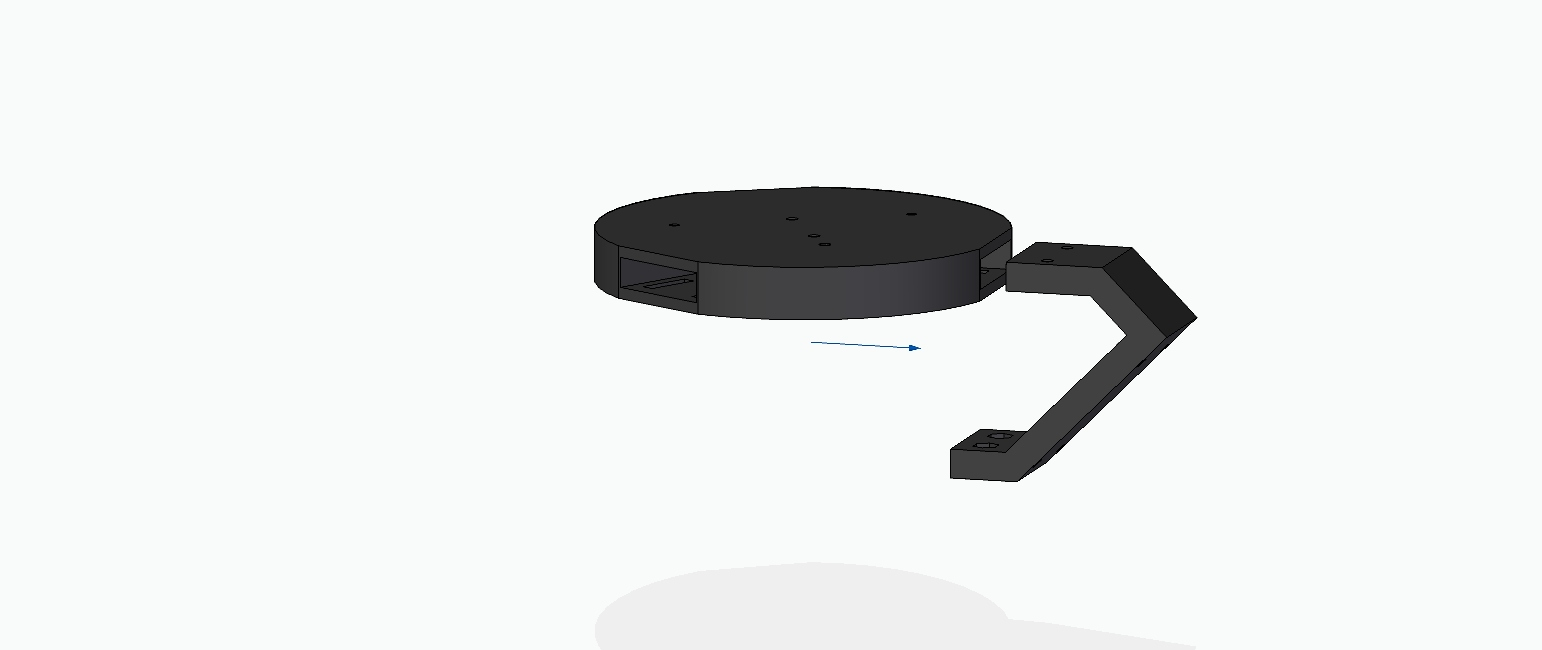
\includegraphics[scale=4.9]{Bilder/Michael/Traeger_Halterung_Explosion.jpg} }
	\caption{Teleskopsystem bestehend aus Tr�gerplatte(links) und Motorenhalter(rechts)}
	\label{fig:Motorenhalter}
\end{figure}

R�cksicht wurde weiterhin auf eine stabile Integration der Motoren in die Gesamtkonstruktion genommen. So soll bei den wirkenden Kr�ften und Momenten, Bewegungen der Unterbaukomponenten relativ zu einander vermieden werden. Integriert wurden die Motoren daher �ber vier M3 Zylinderkopfschrauben an den sogenannten Motorenhaltern, wie in Abbildung \ref{fig:antrieb} dargestellt. Die F�hrungsschiene des Motorenhalters  wird in eine F�hrungsnut der Tr�gerplatte passgenau eingef�hrt und verschraubt.


\begin{figure}[!htbp]%
	\centering
	{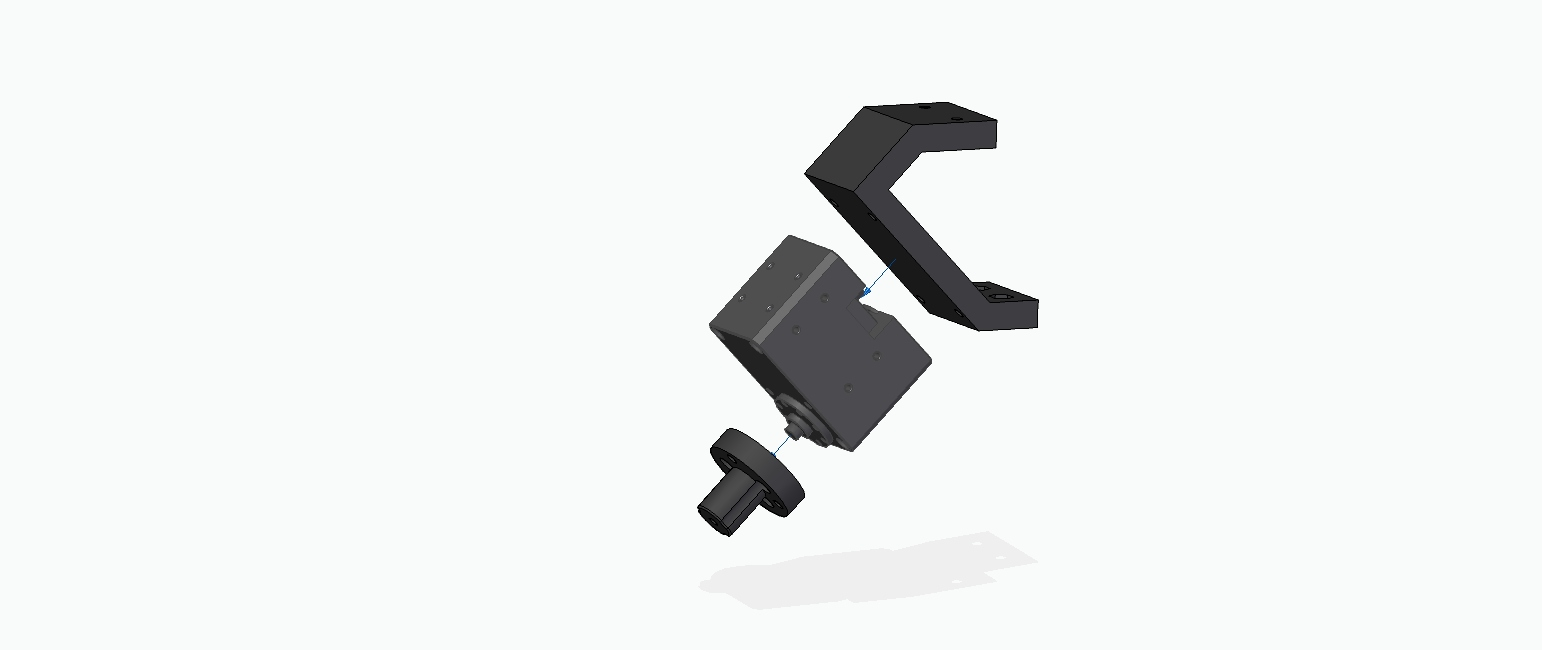
\includegraphics[scale=4.8]{Bilder/Michael/Motor_Mitnehmer_Halterung_Explosion.jpg} }
	\caption{Antriebsvorrichtung bestehend aus Mitnehmer (unten), Motor (mitte) und Motorenhalter (oben). }
	\label{fig:antrieb}
\end{figure}

Um die R�der, dargestellt in Abbildung \ref{fig:wheel} an die Motorwellen zu befestigen, sind spezielle Mitnehmer konstruiert worden, die in Abbildung \ref{fig:antrieb} dargestellt sind.

Wichtige Kriterien, die es hierbei zu erf�llen gab, waren eine spielfrei �bertragung der Momente und Kr�fte sowie eine m�glichst kurze Distanz zwischen den R�dern und den Motoren.

Nach einigen Tests hat sich herausgestellt, dass die gew�nschte Stabilit�t es Unterbaus nicht gegeben war. Die Konstruktion musste also noch verst�rkt werden. Um die n�tige Stabilit�t herzustellen, sind die Motorenhalter um eine Anflanschfl�che erweitert worden. So k�nnen die Motorenhalter �ber ein Y-f�rmiges Verbindungsst�ck, dargestellt in Abbildung \ref{fig:kreisring}, miteinander gekoppelt werden. Hierbei wurde eine flexible Anpassung an unterschiedlichen Ballradien ber�cksichtigt.
\begin{figure}[!htbp]%
	\centering
	{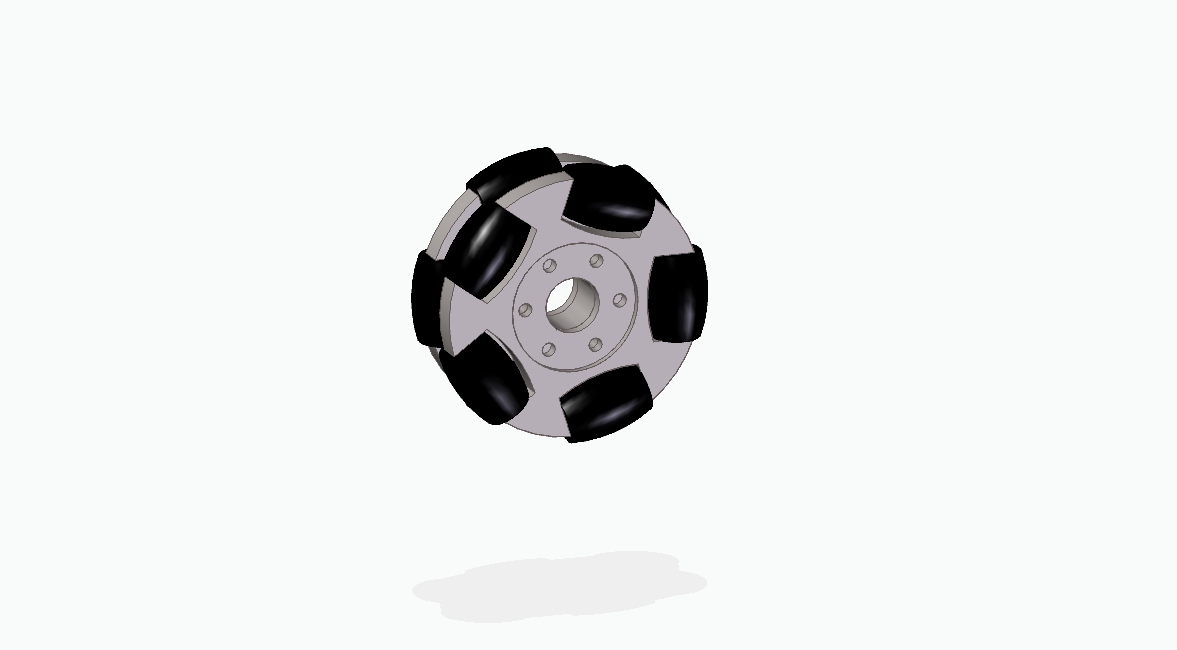
\includegraphics[scale=6.4]{Bilder/Michael/Wheel2_Double.jpg} }
	\caption{Modell eines omnidirektionalen Rades}
	\label{fig:wheel}
\end{figure}

\begin{figure}[!htbp]%
	\centering
	{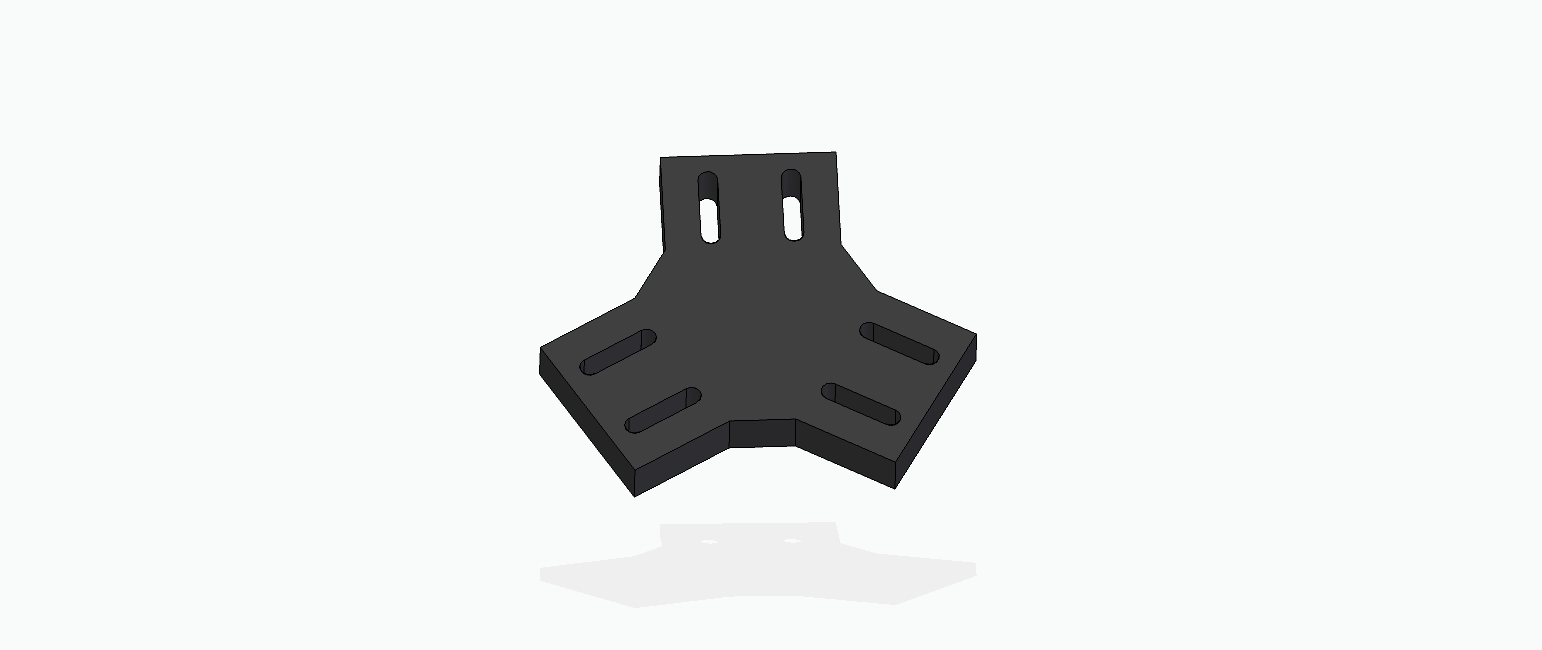
\includegraphics[scale=4.8]{Bilder/Michael/Kreisring_Stabi.jpg} }
	\caption{Y-f�rmiges Verbindungsst�ck des Unterbaus.}
	\label{fig:kreisring}
\end{figure}

\section{Fertigung der Komponenten} \label{sec:Fertigung}
Neben dem Zugang zu einem professionellen CAD-Tool bestand auch Zugang zu einem 3D-Drucker der Firma Oktoprint. Dies erm�glichte eine kosteng�nstige und schnelle Fertigung der konstruierten Bauteile. Verwendete wurde dabei das Filament Polylactide (PLA). PLA ist ein sehr verbreiteter biokompatibler Kunstoff, der eine hohe Oberfl�chenh�rte, hohe Steifigkeit und eine hohe Zugfestigkeit bietet \cite{pla}. 

Der fertige Entwurf wurde schlie�lich als .stl exportiert und in das 3D-Druckprogramm CURA geladen. Mit CURA konnte anschlie�end die F�lldichte, die Qualit�t, Druckgeschwindigkeit und der Einsatz von St�tzhilfen f�r den jeweiligen Druck eingestellt werden. Die gew�nschten Genauigkeiten konnten mittels dieser Fertigungsweise eingehalten werden. So hat der Druck auch an kritischen Stellen wie der Einschubverbindung zwischen Tr�gerplatte und Motorenhalter �berzeugt. Es war nach Einschub und Verschraubung der Motorenhalter mit der Tr�gerplatte kein Spiel vorhanden. 
\chapter{Modellbildung und Regelung} \label{ch:Modellierung}
In diesem Kapitel wird anhand des Vorgehens in \cite{ETHZ} die Modellbildung des Ballbot's erl�utert, die f�r die Auslegung eines geeigneten Regler ben�tigt wird. Im Anschluss kann mit Hilfe der Simulationsumgebung MATLAB/Simulink sowohl das Modell als auch der Regler verifiziert werden. 

\section{Model}\label{sec:Model}
F�r die Modellbildung wird der dreidimensionale Ballbot in die $yz$-, $xz$- und $xy$-Ebenen aufgeteilt, das in Abbildung \ref{fig:2D_Modell} dargestellt ist. In jeder Ebene wird das System vereinfacht als Zusammensetzung von drei starren K�rpern, bestehend aus einer Kugel, einem virtuellem Rad und einem K�rper betrachtet. Das Modell jeder Ebene besitzt somit zwei Freiheitsgrade, die sich in eine Translation bzw. Rotation des Balles und eine Rotation des K�rpers aufteilen lassen \cite{ETHZ}.

\begin{figure}[h!]%
	\centering
	\subfloat[Darstellung der $yz$-Ebene mit Parameter (gleicher Aufbau auch f�r die $xz$-Ebene]{ \scalebox{.7}{{\input{./Bilder/Florian/Modell_2.pdf_tex} }}}%
	\qquad \qquad
	\subfloat[Darstellung der $xz$-Ebene]{ \scalebox{.7}{{\input{./Bilder/Florian/xyPlane.pdf_tex}}}}%
	\caption{Aufteilung des Ballbot's in drei unabh�ngigen Ebenen \cite{ETHZ}}%
	\label{fig:2D_Modell}%
\end{figure}%\newline

Um m�glichst vereinfachte Modelle der drei Ebenen zu erhalten, werden weitere Annahmen getroffen, die im Folgenden erl�utert werden \cite{ETHZ}: 
\begin{itemize}
	\item Kein Schlupf: Das System besitzt zwei Kontaktpunkte, in denen ein Schlupf auftreten kann. Hierzu z�hlt zum einen der Kontaktpunkt von Ball und Boden und zum anderen der Kontaktpunkt zwischen R�dern und Ball. Damit kein Schlupf auftritt, m�ssen die angelegten Drehmomente begrenzt werden.
	\item Keine Reibung: F�r die Modellierung wird ein reibungsfreies System angenommen. Lediglich bei der Rotation des Balles um die $z$-Achse wird die Reibung ber�cksichtigt. 
	\item Keine Deformation: Der Ball wird als nicht deformierbar angenommen. 
	\item Schnelle Motorendynamik: F�r die Gleichgewichtsstabilisierung des Roboters ist es wichtig, dass die Motoren eine schnellere Dynamik als das Gesamtsystem aufweisen. 
	\item Horizontale Bewegung: Die Ballbewegung wird f�r die horizontale Bewegung auf einer flachen Oberfl�che ohne starken Neigungen eingeschr�nkt. Somit wird die vertikale Bewegung vernachl�ssigt. 
\end{itemize}
Mit den getroffenen Annahmen ist es m�glich, das Modell des Ballbot's aufzustellen. 

\section{Minimalkoordinaten}
F�r die Beschreibung der einzelnen Modellebenen werden bestimmte Winkel verwendet, die in Abbildung \ref{fig:2D_Modell} zu sehen sind. Dabei beschreiben die Winkel $\vartheta_{xyz}$ die Orientierung des Roboters, die Winkel $\varphi_{xyz}$ die Orientierung des Balles und die Winkel $\psi_{xyz}$ die Orientierung des virtuellen Rades in den jeweiligen planaren Ebenen. Unter Verwendung folgender minimalen Koordinaten 
\begin{align}
	\mathbf{q}_{yz} &= \begin{bmatrix} \varphi_{x} \\ \vartheta_{x} \end{bmatrix} &
	\mathbf{q}_{xz} &= \begin{bmatrix} \varphi_{y} \\ \vartheta_{y} \end{bmatrix} &
	\mathbf{q}_{xy} &= \begin{bmatrix} \varphi_{z} \\ \vartheta_{z} \end{bmatrix}
\end{align}
kann das komplette System mit Hilfe von Energien beschrieben werden \cite{ETHZ}. 

\section{Energien}
Das Aufstellen der Bewegungsgleichungen f�r die einzelnen Ebenen wird anhand der LAGRANGEschen Gleichungen zweiter Art durchgef�hrt. Dazu m�ssen im Voraus die potentiellen und kinetischen Energien der einzelnen K�rper aufgestellt werden. Dabei ist darauf zu achten, dass die Formeln der potentiellen und kinetischen Energien f�r die $yz$- und der $xz$-Ebene identisch sind und sich nur durch die entsprechenden Winkel der Ebenen unterscheiden. Damit der Ballbot zun�chst seine Gleichgewichtslage halten kann, hat die Orientierung um die $z$-Achse eine vernachl�ssigbare Bedeutung. Aus diesem Grund wird die $xy$-Ebene f�r den Entwurf eines Reglers nicht ber�cksichtigt und somit auch f�r die Herleitung der Bewegungsgleichungen. \newline
Die Herleitung der Bewegungsgleichungen wird nachfolgend f�r die $yz$-Ebene durchgef�hrt.  %Zun�chst werden die kinetischen und potentiellen Energien des Balles in den entsprechenden Ebenen betrachten. 
Die kinetische und potentielle Energie des Balles entsprechen folgenden Formeln: 
\begin{align} 
	T_{S,yz} &= \frac{1}{2} \cdot m_{S} \cdot (r_{S} \cdot \dot \varphi_{x})^2 + \frac{1}{2} \cdot I_{S} \cdot \dot\varphi_{x}^2 \\
	V_{S,yz} &=0
\end{align}
%\begin{equation}
	%T_{S,xy} =\frac{1}{2} \cdot I_{S} \cdot \dot\varphi_{z}^2
%\end{equation}
Die potentielle Energie kann mit Null gleichgesetzt werden, da der Ursprung des Weltkoordinatensystems in den Mittelpunkt des Balles gelegt wird.

Die kinetische und potentielle Energie des virtuellen Rades in der $yz$-Ebene wird mit 
\begin{align}
\begin{split}
	T_{W,yz} &= \frac{1}{2} \cdot m_{W} \cdot ((r_{S} \cdot \dot \varphi_{x})^2 + 2 \cdot (r_{S}+r_{W}) \cdot \cos(\vartheta_{x})\cdot \dot \vartheta_{x} \cdot (r_{S}\cdot\dot\varphi_{x})+(r_{S} + r_{W})^2\cdot\dot\vartheta_{x}^2) \\ & + \frac{1}{2} \cdot I_{W}\cdot(\frac{r_{S}}{r_{W}}\cdot(\dot\varphi_{x}-\dot\vartheta_{x})-\dot\vartheta_{x})^2 	\end{split} \\
	V_{W,yz} &= m_{W} \cdot g \cdot (r_{S} + r_{W})\cdot \cos(\vartheta_{x})
\end{align}
berechnet. Dabei besteht die kinetische Energie ebenfalls aus einem translatorischem und rotatorischem Teil und einem zus�tzlichem Kopplungsteil. Die potentielle Energie ist abh�ngig von dem Winkel $\vartheta_{x}$.

F�r den K�rper bzw. den Roboter sind die Formeln f�r die kinetische und potentielle Energie �hnlich zu denen des virtuellen Rads und lauten: 
\begin{align}
T_{B,yz} &= \frac{1}{2} \cdot m_{A} \cdot ((r_{S} \cdot \dot \varphi_{x})^2 + 2 \cdot l \cdot \cos(\vartheta_{x})\cdot \dot \vartheta_{x} \cdot (r_{S}\cdot\dot\varphi_{x}) + l^2\cdot\dot\vartheta_{x}^2)+\frac{1}{2} \cdot I_{A}\cdot\dot\vartheta_{x}^2 \\
V_{B,yz} &= m_{A} \cdot g \cdot l \cdot \cos(\vartheta_{x})
\end{align}

Die Gesamtenergie setzt sich aus allen Teilenergien der einzelnen Komponenten des Ballbot's zusammen \cite{ETHZ}. 

\subsection{Externe Kr�fte und Drehmomente}
Die Krafteinwirkung auf das Gesamtsystem erfolgt �ber das Drehmoment der Motoren. F�r die einzelnen Ebenen der Modellbildung wirkt daher �ber das entsprechende virtuelle Rad ein virtuelles Drehmoment $T_{x,y,z}$. Daher kann die resultierende Krafteinwirkung in zwei Teile aufgeteilt werden. Ein Teil resultiert aus dem Effekt der Motordrehmomente und der andere Teil beschreibt die Krafteinwirkung durch das erzeugte Gegendrehmoment. Die gesamte Krafteinwirkung kann durch die Summe von
\begin{align}
\mathbf{f}_{NP,yz1} &= \begin{bmatrix}  \frac{r_{S}}{r_{W}} \cdot T_{x} \\ -\left(1+\frac{r_{S}}{r_{W}}\right) \cdot T_{x} \end{bmatrix}&  
	\mathbf{f}_{NP,yz2} &= \begin{bmatrix} 0 \\ T_{x} \end{bmatrix}
 \end{align}

f�r die $yz$-Ebene angeben werden und f�r die Modellierung als Kraftanregung genutzt werden.

Ein weiterer, wichtiger Punkt in Bezug auf die sp�tere Simulation und Implementierung ist die Umrechnung von den virtuellen Drehmomenten $T_{x,y,z}$ auf die realen Drehmomente $T_{1,2,3}$ der Motoren. Die Umrechnung erfolgt mit 
\begin{equation}
\label{eq:realeDrehmomente}
\begin{bmatrix} T_{1}\\ T_{2} \\ T_{3} \end{bmatrix} = \frac{1}{3} \cdot
\begin{bmatrix} \frac{2 \cdot \cos{\beta}}{\cos{\alpha}} & \frac{- 2 \cdot \sin{\beta}}{\cos{\alpha}} & 1 \\ 
\frac{-\sin{\beta} \cdot \sqrt{3} - \cos{\beta}}{\cos{\alpha}} & \frac{\sin{\beta} - \cos{\beta}\cdot \sqrt{3}}{\cos{\alpha}} & 1 \\
\frac{\sin{\beta} \cdot \sqrt{3} - \cos{\beta}}{\cos{\alpha}} & \frac{\sin{\beta} + \cos{\beta}\cdot \sqrt{3}}{\cos{\alpha}} & 1\end{bmatrix} \cdot 
\begin{bmatrix} T_{x}\\ T_{y} \\ T_{z} \end{bmatrix}
\end{equation} 
F�r die genaue Herleitung der in diesem Kapitel beschriebenen Gleichungen ist auf \cite{ETHZ} verwiesen. 

\section{Bewegungsgleichungen}
Mit den kinetischen und potentiellen Energien k�nnen nun die Bewegungsgleichungen des Ballbot's f�r die jeweiligen Ebenen mit Hilfe der LAGRANGEschen Gleichungen zweiter Art hergeleitet werden. Als Beispiel wird auch hier die Herleitung f�r die $yz$-Ebene angegeben.\newline
Zun�chst wird aus den einzelnen Summen der kinetischen und potentiellen Energien die LANGRANGEsche Funktion gebildet \cite{MatPrakt}. 	
\begin{align}
		L = T - V 
\end{align}
Die Bewegungsgleichungen f�r den Ballbot resultieren aus dem L�sen der LAGRANGEschen Gleichungen zweiter Art. 
	\begin{align}
		\frac{d}{dt}\left(\frac{\partial L}{\partial \dot{\mathbf{q}}}\right)^{T} - \left(\frac{\partial L}{\partial \mathbf{q}}\right)^{T} = \mathbf{f}_{NP,yz}
\end{align}

Mit mathematische Umformungen k�nnen diese Bewegungsgleichungen in eine Matrixform �berf�hrt werden:
\begin{align}
	\mathbf{M}_x(\mathbf{q}, \dot{\mathbf{q}}) \cdot \ddot{\mathbf{q}}+\mathbf{C}_x(\mathbf{q}, \dot{\mathbf{q}})+\mathbf{G}_x(\mathbf{q})=\mathbf{f}_{NP, yz}
\end{align}
Hierbei ist:
\begin{align}
\label{eq:MatrizenDGL}
\mathbf{M}_{x} &=\begin{bmatrix} m_{tot} \cdot r_{S}^{2} + I_{S} + (\frac{r_{S}}{r_{W}})^{2} \cdot I_{W}  & -\frac{r_{S}}{r_{W}^2}\cdot r_{tot} \cdot I_{W} + \gamma \cdot r_{S} \cdot \cos{\vartheta_{x}} m_{tot} \\ -\frac{r_{S}}{r_{W}^2}\cdot r_{tot} \cdot I_{W} + \gamma \cdot r_{S} \cdot \cos{\vartheta_{x}} m_{tot}	& \frac{r_{S}^2}{r_{W}^2} \cdot I_{W} + I_{B} + m_{b}\cdot l^2 + m_{W}\cdot r_{tot}^2  \\ \end{bmatrix} &,& \mathbf{M}_{x} \in \mathbb{R}\textsuperscript{2$\times$2} \nonumber \\ 
\mathbf{C}_{x} &=\begin{bmatrix}  -r_{S} \cdot \gamma \cdot \sin{\vartheta_{x}} \cdot \dot \vartheta_{x}^{2} \\ 0 \\ \end{bmatrix} &,& \mathbf{C}_{x} \in \mathbb{R}\textsuperscript{\textit{2$\times$1}} \nonumber \\
\mathbf{G}_{x} &=\begin{bmatrix}  0 \\ -g\cdot \sin{\theta_{x}}\cdot \gamma  \\ \end{bmatrix}  &,&  \mathbf{G}_{x} \in \mathbb{R}\textsuperscript{\textit{2$\times$1}} \nonumber \\ 
\end{align}
mit den Substitutionen:
\begin{align}
	m_{tot}&=m_{B}+m_S+m_W \nonumber\\
	r_{tot}&=r_S+r_W \nonumber\\
	\gamma&=l\cdot m_B+(r_S+r_W)m_W
\end{align}	

\section{Zustandsraumdarstellung}
Bei den hergeleiteten Bewegungsgleichungen f�r die $yz$-Ebene handelt es sich um nichtlineare Funktionen. Um ein lineares Zustandsraummodell zu erhalten, m�ssen zun�chst die Zust�nde bzw. der Zustandsvektor festgelegt werden. Mit $\mathbf{x} = \begin{bmatrix}\varphi_{x} \quad \vartheta_{x} \quad  \dot\varphi_{x} \quad \dot\vartheta_{x}\end{bmatrix}^{T}$ k�nnen die nichtlinearen Funktionen in folgende Form �berf�hrt werden.
\begin{equation}
\dot{\mathbf{x}}_{nl} = \begin{bmatrix} \mathbf{q}\\ \dot{\mathbf{q}}\\ \end{bmatrix} = \begin{bmatrix} \dot{\mathbf{q}}\\  \mathbf{M_{x}}^{-1}\cdot (\mathbf{f}_{NP,yz}-(\mathbf{C_{x}}+\mathbf{G_{x}}))\\ \end{bmatrix}
\end{equation}

Das Ziel dieser Arbeit ist das Auslegen eines Reglers, damit der Roboter innerhalb eines kleinen Bereiches um den Arbeitspunkt $\mathbf{x}_{0}= \left[0 \quad 0 \quad 0 \quad 0\right]^{T}$ auf dem einen Ball balanciert. Hierzu muss zun�chst das nichtlineare Modell um den Arbeitspunkt mit der Taylor-Reihenentwicklung linearisiert werden, um die lineare Zustandsraumdarstellung 
\begin{align}
\label{eq:LZRD}
\dot{\mathbf{x}} &=\mathbf{A}\cdot\mathbf{x} + \mathbf{B} \cdot \mathbf{u} \nonumber \\
\mathbf{y} &=\mathbf{C} \cdot \mathbf{x} + \mathbf{D} \cdot \mathbf{u} 
\end{align}
zu erhalten. Mit den zum Roboter dazugeh�rigen Parametern (siehe Anhang \ref{ch:Parameterliste}) und dem eingesetzten Arbeitspunkt lauten die konkreten Matrizen f�r die lineare Zustandsraumdarstellung der $yz$-Ebene folgenderma�en:

\begin{align}
%\label{eq:konkZRD}
\mathbf{A} &=\begin{bmatrix} 0 & 0 & 1 & 0 \\ 0 & 0 & 0 & 1 \\ 0 & 0.4886 & 0 & 0 \\ 0 & 17.1119 & 0 & 0\end{bmatrix} & 
\mathbf{B} &=\begin{bmatrix} 0 \\ 0 \\ 63.5516 \\ -10.6945 \end{bmatrix} &
\mathbf{C} &=\begin{bmatrix} 1 & 0 & 0 & 0 \\ 0 & 1 & 0 & 0 \\ 0 & 0 & 1 & 0\\ 0 & 0 & 0 & 1 \end{bmatrix} &
\mathbf{D} &=\begin{bmatrix} 0 \\ 0 \\ 0\\ 0 \end{bmatrix} \nonumber 
\end{align} 

Damit der Roboter auf einen Ball die eigene Gleichgewichtslage einhalten kann, ist es zun�chst nebens�chlich, welche Position und Geschwindigkeit der Ball dabei einnimmt. Vielmehr von Bedeutung ist die aufrechte Haltung des Ballbots. Dadurch sind f�r den sp�teren Entwurf einer Regelung nur die Zust�nde des Roboters von Bedeutung und die Zust�nde f�r den Ball m�ssen nicht f�r eine Regelung ber�cksichtigt werden. Mit dem neuem Zustandsvektor $\mathbf{x}^{*}=\left[\vartheta_{x} \quad \dot{\vartheta_{x}}\right]^{T}$ wird die Ordnung des Modells \ref{eq:LZRD} reduziert, das zu folgenden Zustandsraummatrizen f�hrt: 

\begin{align}
%\label{eq:redZRD}
\mathbf{A}^{*} &=\begin{bmatrix} 0 & 1 \\ 17.1119 & 0 \end{bmatrix} & 
\mathbf{B}^{*} &=\begin{bmatrix} 0 \\ -10.6945 \end{bmatrix} &
\mathbf{C}^{*} &=\begin{bmatrix} 1 & 0 \\ 0 & 1 \end{bmatrix} &
\mathbf{D}^{*} &=\begin{bmatrix} 0 \\ 0 \end{bmatrix} \nonumber 
\end{align}

Die Pr�fung auf Stabilit�t des Modells erfolgt anhand der Lage der Eigenwerte. Das urspr�ngliche und das reduzierte Modell besitzt folgende Eigenwerte: 

\begin{align}
\label{eq:EW}
\mathbf{\lambda} &=\begin{pmatrix} 0 \\ 0 \\  4.1367\\ -4.1367 \end{pmatrix} & 
\mathbf{\lambda}^{*} &=\begin{pmatrix} 4.1367 \\ -4.1367 \end{pmatrix} & 
\end{align}

Das urspr�nglich Modell besitzt zwei Eigenwerte $\lambda_{1,2} = 0$ auf der imagin�ren Achse und einen instabilen Eigenwert $\lambda_{3} = 4.1367$ in der rechten Halbebene des Bildbereiches. Somit ist das Modell instabil. Bei dem reduzierten Modell handelt es sich ebenfalls um ein instabiles System, da es auch einen Eigenwert $\lambda_{1}^{*} = 4.1367$ besitzt.

Die Untersuchung der Steuer- und Beobachtbarkeit erfolgt in beiden Modelle mit den entsprechenden Kriterien von KALMANN. In beiden F�llen besitzen die Steuerbarkeits- und Beobachtbarkeitsmatrizen vollen Rang, wodurch beide Modelle vollst�ndig steuer- und beobachtbar sind. Mit diesen Systemeigenschaften ist es mit Hilfe eines Reglers m�glich, das entsprechende instabile System zu stabilisieren. Das Auslegen eines geeigneten Regler wird nachfolgend erl�utert \cite{ETHZ}\cite{MGR}.   
  
\section{Reglerentwurf}

\begin{figure}[h!] 
		\centering
\begin{tikzpicture}[auto, thick, node distance=0.5cm]
% Definition of blocks:
\usetikzlibrary{positioning,arrows,calc}
\tikzset{%
  block/.style    = {draw, thick, rectangle, minimum height = 3em, minimum width = 3em, node distance = 1.5cm},
  sum/.style      = {draw, circle, node distance = 1.5cm}, % Adder
	%join/.style			= {coordinate}, 
  input/.style    = {coordinate}, % Input
  output/.style   = {coordinate} % Output
}
\draw
	node [input](w){0}
	node [sum, right = of w](s1){}
	node [block, right = of s1] (B) {$\mathbf{B}$}
	node [sum, right = of B] (s2) {}
	node [block, right = of s2] (I) {$\mathbf{\int}$}
	node [input, right = of I] (temp) {}
	node [block, right = of temp] (C) {$\mathbf{C}$}
	node [output, right = of C] (y) {}
	node [block, below = of I] (A) {$\mathbf{A}$}
	node [block, below = of A] (K) {$\mathbf{K}$};
	
	
	\draw[->](w) -- node {$\mathbf{w} = 0$}(s1);	
	\draw[->](s1) --node {$\mathbf{u}$} (B);
	\draw[->](B) -- (s2);
	\draw[->](s2) -- node {$\dot{\mathbf{x}}$}(I);
	\draw[-](I) -- node {$\dot{\mathbf{x}}$}(temp);
	\draw[->](temp) --(C);
	\draw[->](C) -- node (y_temp) {$\mathbf{y}$}(y);
	\draw[->](temp) |- node[very near end] {} (A);
	\draw[->](temp) |- node[very near end] {} (K);
	\draw[->](A) -| node[pos=0.99] {$+$} node[very near end] {} (s2);
	\draw[->](K) -| node[pos=0.99] {$-$} node[very near end] {} (s1);
	%
\end{tikzpicture}
\caption{Linearisierte Zustandsraumdarstellung mit r�ckgekoppelter Reglerverst�rkung \cite{ETHZ}}
	\label{fig:LQR1}
\end{figure}

Der Entwurf eines geeigneten Reglers zur Stabilisierung der Gleichgewichtslage des Roboters wird im Folgenden auf das reduzierte Model beschr�nkt. F�r die beiden Modelle der $yz$- und $xz$-Ebene wird jeweils ein linear-quadratischer Zustandsregler (LQR) ausgelegt, dessen Funktionsweise in Abbildung \ref{fig:LQR1} dargestellt ist und auf der Minimierung des G�tema�
\begin{equation}
	J = \int_{0}^{\infty} \mathbf{x}^{T}(t)\cdot \mathbf{Q} \cdot \mathbf{x}(t) + \mathbf{u}^{T}(t)\cdot \mathbf{R} \cdot \mathbf{u}(t)
\end{equation}
durch einen vorgegebenen Stellgr��enverlauf basiert. In das G�teintegral geht quadratisch der Trajektorienverlauf $\mathbf{x}(t)$ und der Stellgr��enverlauf $\mathbf{u}(t)$ ein. Dabei handelt es sich bei der symmetrischen und positiv semidefiniten Matrix $\mathbf{Q}$ um eine Gewichtungsmatrix f�r den Trajektorienverlauf. F�r ein rasches Einschwingen eines bestimmten Zustandes ist dieser entsprechend mit einem gr��eren Gewicht in der Gewichtungsmatrix zu versehen. Die symmetrische und positiv definite Matrix $\mathbf{R}$ gewichtet dagegen die Stellgr��e. M�ssen Stellgr��enbeschr�nkungen ber�cksichtigt werden, sind die entsprechenden Stellgr��en in dieser Matrix mit gr��eren Gewichten zu versehen. Wird insgesamt die Gewichtungsmatrix $\mathbf{Q}$ im Verh�ltnis zur der Gewichtungsmatrix $\mathbf{R}$ vergr��ert, f�hrt das zu einem schnelleren Einschwingen der Zust�nde mit h�heren Stellgr��en. Im umgekehrten Fall stabilisiert sich das System langsamer, da die H�he der Stellgr��en abnimmt \cite{SDRTII}\cite{AUGS}.

Das Regelgesetz, das aus der Minimierung des G�tema� resultiert, ergibt sich zu 
 \begin{align}
\label{eq:Regelgesetz}
\mathbf{u}(t) &= -\mathbf{K}\cdot\mathbf{x}(t) &&mit & \mathbf{K} &=\mathbf{R}^{-1}\cdot\mathbf{B}^{T}\cdot\mathbf{P}. 
\end{align}
Die symmetrisch positiv definite Matrix $\mathbf{P}$ errechnet sich aus dem algebraischen Teil der Riccati-Differentialgleichung 
\begin{align}
	\mathbf{A}^{T} \cdot \mathbf{P} + \mathbf{P} \cdot \mathbf{A} - \mathbf{P} \cdot \mathbf{B} \cdot \mathbf{R}^{-1} \cdot \mathbf{B}^{T} \cdot \mathbf{P} = - \mathbf{Q}.
\end{align}
Das L�sen der Riccati-Differentialgleichung und somit die Berechnung der Reglermatrix $\mathbf{K}$ kann mit Hilfe 
von MATLAB und dem dazugeh�rigen Befehl \textit{lqr()} durchgef�hrt werden. Zu Beginn werden die einzelnen Gewichtungen der einzelnen Zust�nde und Stellgr��en zu 
 \begin{align}
%\label{eq:redZRD}
\mathbf{Q} = \begin{bmatrix}  100 & 0 \\ 0 & 50 \end{bmatrix} \nonumber & &
\mathbf{R} = 200 \nonumber 
\end{align}
festgelegt. Mit dieser Konfiguration werden die einzelnen Verst�rkungsfaktoren des Regler zu 
\begin{equation}
	\mathbf{K} = \begin{bmatrix} -3.3494 & -0.9362 \end{bmatrix}
\end{equation}
 berechnet.
 
Diese Verst�rkungsfaktoren sind nicht ideal f�r das System. Durch manuelles Anpassen der Werte kann das Balancieren des Roboters um die Gleichgewichtslage schrittweise angepasst werden, das schlie�lich zu folgende Reglermatrix 
\begin{equation}
	\mathbf{K} = \begin{bmatrix} -8.6953 & -2.0932 \end{bmatrix}
\end{equation}
f�hrt. 

\section{Simulation des Modells}
Mit dem Aufbau und Durchf�hrung einer Simulation mittels MATLAB/Simulink k�nnen sowohl die nichtlinearen Bewegungsgleichungen und somit das dynamische Systemverhalten des Ballbots als auch der entworfene Zustandsregler verifiziert werden. Weiterhin besteht die M�glichkeit, sowohl die Verst�rkungsfaktoren des Regler zu optimieren, um die Dynamik des Systems zu erh�hen oder Stellgr��en zu beschr�nken, als auch Grenzsituationen zu testen. Dadurch entf�llt das Testen am realen System, das zeitaufwendig ist und zu eventuellen Besch�digungen f�hren kann \cite{M&S}. \newline
Im Folgenden wird zun�chst die allgemeine Implementierung in MATLAB/Simulink erl�utert, die dann schrittweise an die realen Gegebenheiten angepasst wird.

\subsection{Implementierung ideales Modell}
Ein wichtiger Bestandteil im Aufbau der Simulation besteht in dem L�sen der nichtlinearen Differentialgleichungen. F�r diese Aufgabe wird in MATLAB/Simulink f�r jede Ebene ein MATLAB-Funktion-Block eingesetzt. Die Programmierung bzw. Parametrierung dieses Blockes erfolgt nicht grafisch, sondern mit Unterst�tzung eines Editors. Als Eingang wird dem Block in jedem Berechnungsschritt der aktuelle Zustandsvektor $\mathbf{x}$ und das aktuelle, virtuelle Drehmoment $T$  der entsprechenden Ebene �bergeben. Mit den Werten wird dann die Bewegungsdifferentialgleichung f�r den aktuellen Schritt berechnet. Als R�ckgabewert bzw. Ausgang wird die berechnete, zeitliche Ableitung des Zustandsvektors $\dot{\mathbf{x}}$ zur�ckgegeben. Die Abbildung \ref{fig:simple_Simulink} (a) zeigt die Funktionsweise des L�sens der nichtlinearen Bewegungsgleichungen f�r die $yz$-Ebene \cite{MatPrakt}.

\begin{figure}[!htbp]%
	\centering
	\subfloat[Aufbau Matlab-Funktion-Block mit anschlie�enden Integrierer f�r $yz$-Ebene]{{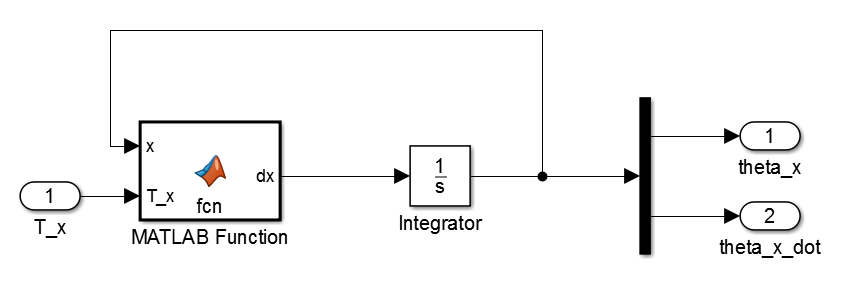
\includegraphics[width=0.45\textwidth]{./Bilder/Florian/Matlab_Funktion_Block.PNG} }}%
	\qquad 
	\subfloat[Aufbau Gesamtsystem inklusive Regler f�r $yz$-Ebene]{{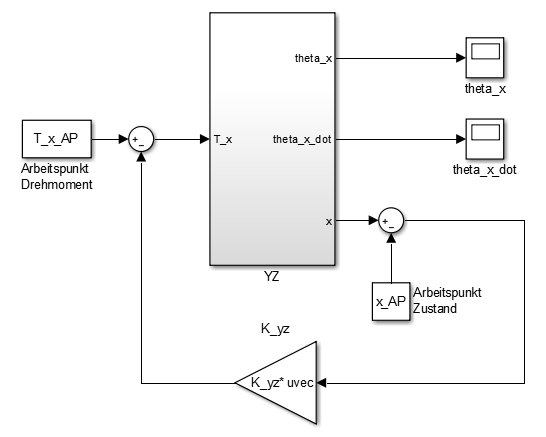
\includegraphics[width=0.45\textwidth]{./Bilder/Florian/Gesamtsystem.PNG} }}%
	\caption{Aufbau Simulinkmodell f�r $yz$-Ebene bestehen aus Subsystem und Gesamtsystem mit Regler}%
	\label{fig:simple_Simulink}%
\end{figure}

Mit der Hinzunahme der Reglerverst�rkungsfaktoren als Zustandsr�ckf�hrung ergibt sich das Gesamtsystem, das in der Abbildung \ref{fig:simple_Simulink} (b) abgebildet ist. Hier ist zu beachten, dass der Zustandsregler f�r das linearisierte Modell ausgelegt wurde. Deshalb muss der Arbeitspunkt des Zustandes vor der R�ckf�hrung abgezogen werden. Nach dem Regler muss der Arbeitspunkt des Drehmomentes analog wieder auf das $\Delta u$ addiert werden. Im Anhang \ref{ch:gesamtbild} ist eine komplette �bersicht des Simulink-Simulationsaufbaus zu sehen.

\subsection{Reale Gegebenheiten}
Die inertiale Messeinheit liefert in der Realit�t verrauschte Signale, die f�r die Berechnung des Regelgesetzes ben�tigt werden. Die St�rke dieses Rauschen kann dem Datenblatt der IMU entnommen werden und in der Simulation durch ein wei�es Rauschen integriert werden. Die Abbildung \ref{fig:Rauschen} zeigt den Einfluss des Rauschen auf den Winkel $\vartheta_{x}$ und das reale Drehmoment $T_{1}$ in der Simulation.  
\begin{figure}[h!]
\centering
% This file was created by matlab2tikz.
%
%The latest updates can be retrieved from
%  http://www.mathworks.com/matlabcentral/fileexchange/22022-matlab2tikz-matlab2tikz
%where you can also make suggestions and rate matlab2tikz.
%
\definecolor{mycolor1}{rgb}{0.00000,0.44700,0.74100}%
%
\begin{tikzpicture}

\begin{axis}[%
width=0.951\figW,
height=0.419\figH,
at={(0\figW,0.581\figH)},
scale only axis,
xmin=0,
xmax=4,
xtick={0,1,2,3,4},
xticklabels={\empty},
ymin=-1,
ymax=1,
ytick={-1,-0.5,0,0.5,1},
yticklabels={{-1},{-0,5},{0},{0,5}},
ylabel style={font=\color{white!15!black}},
ylabel={$\vartheta_{x}$ [$^{\circ}$]},
axis background/.style={fill=white},
xmajorgrids,
ymajorgrids
]
\addplot [color=mycolor1, line width=1.2pt, forget plot]
  table[row sep=crcr]{%
0	0\\
0.0058764	0.0115124409775636\\
0.01087	0.0212888198358809\\
0.021739	0.163762797004292\\
0.032609	0.112179406708664\\
0.043478	0.188354145571307\\
0.05	0.194880134857847\\
0.054348	0.199160129587474\\
0.065217	0.174763586670804\\
0.076087	0.118367350896077\\
0.086957	0.125030850053448\\
0.097826	0.157821224668785\\
0.1	0.160479748838192\\
0.1087	0.171045090580405\\
0.11957	0.199572659199968\\
0.13043	0.227023067164686\\
0.1413	0.216285838083934\\
0.15	0.274057172566975\\
0.15217	0.288472790692467\\
0.16304	0.254616714578187\\
0.17391	0.124652697908662\\
0.18478	0.0291555303630271\\
0.19565	0.134496112829009\\
0.2	0.123077063972052\\
0.20652	0.105974273787397\\
0.21739	0.0458612607956565\\
0.22826	-0.00681304114190062\\
0.23913	-0.0536970316018656\\
0.25	-0.0844998156258938\\
0.26087	-0.115439536562958\\
0.27174	-0.129391058874394\\
0.28261	-0.0411481099729103\\
0.29348	-0.0373769017653593\\
0.3	0.00815605421368727\\
0.30435	0.0385205255244404\\
0.31522	0.0839898831882274\\
0.32609	0.103407422865211\\
0.33696	0.0676090198254371\\
0.34783	0.0393180827752625\\
0.35	0.0363415670295579\\
0.3587	0.0244418065824858\\
0.36957	-0.0515891198735793\\
0.38043	0.0759512853225419\\
0.3913	0.134261200133006\\
0.4	0.101161428308298\\
0.40217	0.0928707290127551\\
0.41304	0.033491101998782\\
0.42391	0.023457465090451\\
0.43478	0.067568912779778\\
0.44565	0.0504936245692892\\
0.45	0.0193396174168458\\
0.45652	-0.0273696209156043\\
0.46739	-0.0826949985712317\\
0.47826	-0.0849409931281445\\
0.48913	-0.015845720782138\\
0.5	-0.0190623058440025\\
0.51087	0.0358132999424472\\
0.52174	0.00436490707486564\\
0.53261	0.00255161024483561\\
0.54348	0.0106524313270723\\
0.55	-0.0482172632492344\\
0.55435	-0.0874390891149149\\
0.56522	-0.223063928800332\\
0.57609	-0.19874759997498\\
0.58696	-0.207072676738231\\
0.59783	-0.136226445370305\\
0.6	-0.136736377807971\\
0.6087	-0.138730270935026\\
0.61957	-0.160926655918394\\
0.63043	-0.191196016235156\\
0.6413	-0.150378502910036\\
0.65	-0.124801666935396\\
0.65217	-0.118401728363785\\
0.66304	-0.0649963322796406\\
0.67391	0.0538901183788247\\
0.68478	0.0919769148523511\\
0.69565	-0.00891980695459666\\
0.7	-0.00523689154327524\\
0.70652	0.00025200402703239\\
0.71739	0.0908997541975051\\
0.72826	0.032150953715971\\
0.73913	0.0313213108286216\\
0.75	-0.057662472501966\\
0.76087	-0.0346874378750152\\
0.77174	-0.0628935771715105\\
0.78261	-0.155202807545037\\
0.79348	-0.120865446882847\\
0.8	-0.0439303930260656\\
0.80435	0.00736021583625056\\
0.81522	0.0467653881963729\\
0.82609	0.0370548994844957\\
0.83696	0.222273247043052\\
0.84783	0.182389654923995\\
0.85	0.195647898303322\\
0.8587	0.248520443637995\\
0.86957	0.2934346051983\\
0.88043	0.33731744272737\\
0.8913	0.340090558455803\\
0.9	0.27342118941438\\
0.90217	0.256713740108365\\
0.91304	0.294374255982314\\
0.92391	0.305065648439455\\
0.93478	0.217706773415859\\
0.94565	0.382334736690798\\
0.95	0.418677449635946\\
0.95652	0.473039685237959\\
0.96739	0.471945335849259\\
0.97826	0.399701087461214\\
0.98913	0.358453855789746\\
1	0.335758997524614\\
1.0109	0.330694050615657\\
1.0217	0.274933797993526\\
1.0326	0.217351539582878\\
1.0435	0.182607378886145\\
1.05	0.147897595657119\\
1.0543	0.124813126091299\\
1.0652	0.190485548569194\\
1.0761	0.132467842234246\\
1.087	0.166461428219358\\
1.0978	0.291876159995544\\
1.1	0.279889882921407\\
1.1087	0.231910397157152\\
1.1196	0.258512827585076\\
1.1304	0.218233894587379\\
1.1413	0.200374800113151\\
1.15	0.132055312621752\\
1.1522	0.114986899904805\\
1.163	0.216767122631844\\
1.1739	0.219311055242225\\
1.1848	0.208464964180399\\
1.1957	0.205869465368456\\
1.2	0.201056619889357\\
1.2065	0.193837351670709\\
1.2174	0.127861261561394\\
1.2283	0.117972010017437\\
1.2391	0.178304465844712\\
1.25	0.303100403202157\\
1.2609	0.30442966528686\\
1.2717	0.156961787976089\\
1.2826	0.23930155271434\\
1.2935	0.228764858861884\\
1.3	0.275529674100462\\
1.3043	0.306681389421724\\
1.3152	0.360780064437977\\
1.3261	0.349229235288139\\
1.337	0.296207720926733\\
1.3478	0.374932121977708\\
1.35	0.364424076015009\\
1.3587	0.322317407650845\\
1.3696	0.280273764644145\\
1.3804	0.335432411581389\\
1.3913	0.354087917390849\\
1.4	0.274710344453425\\
1.4022	0.254863086430093\\
1.413	0.239450521741074\\
1.4239	0.226553241772679\\
1.4348	0.213936711123898\\
1.4457	0.231348898517924\\
1.45	0.19620939694255\\
1.4565	0.143554575570028\\
1.4674	0.113875361782251\\
1.4783	0.0267577019904046\\
1.4891	0.0687377466818449\\
1.5	0.136839510211095\\
1.5109	0.121948337115644\\
1.5217	0.141102316206868\\
1.5326	0.179381626499558\\
1.5435	0.205067324455273\\
1.55	0.22423849228035\\
1.5543	0.236998262377914\\
1.5652	0.221385162460599\\
1.5761	0.242962753025226\\
1.587	0.16331588992409\\
1.5978	0.189408387914348\\
1.6	0.203336991913978\\
1.6087	0.259022760022743\\
1.6196	0.244412336246907\\
1.6304	0.240859997917095\\
1.6413	0.352982108846246\\
1.65	0.339890023227507\\
1.6522	0.336589786327553\\
1.663	0.342571465708719\\
1.6739	0.382695700101731\\
1.6848	0.325371272698892\\
1.6957	0.336796051133801\\
1.7	0.362057760321119\\
1.7065	0.399884433955655\\
1.7174	0.41947959054913\\
1.7283	0.425845151653033\\
1.7391	0.323010686582953\\
1.75	0.24946582399996\\
1.7609	0.120997227175727\\
1.7717	0.0555373720398258\\
1.7826	0.0695570763288819\\
1.7935	0.0605845572571332\\
1.8	0.0229796182893119\\
1.8043	-0.0020015134657305\\
1.8152	0.138260445543019\\
1.8261	0.0990930506678759\\
1.837	0.0995113098583214\\
1.8478	0.0960964813993417\\
1.85	0.0975059575753635\\
1.8587	0.103206887636915\\
1.8696	0.151982784736402\\
1.8804	0.0130703132225243\\
1.8913	-0.0817725365210711\\
1.9	-0.164639422430842\\
1.9022	-0.185294550945308\\
1.913	-0.164032087168003\\
1.9239	-0.166203597211549\\
1.9348	-0.16813446498114\\
1.9457	-0.164713906944209\\
1.95	-0.137910941287989\\
1.9565	-0.0976090899784871\\
1.9674	-0.119920066520881\\
1.9783	-0.217168193088436\\
1.9891	-0.27933411386013\\
2	-0.346650925210051\\
2.0109	-0.425048740317801\\
2.0217	-0.417955522814082\\
2.0326	-0.508362533307774\\
2.0435	-0.520847283663675\\
2.05	-0.469613397623077\\
2.0543	-0.435344791896302\\
2.0652	-0.505056566829869\\
2.0761	-0.522508861269554\\
2.087	-0.57605176722453\\
2.0978	-0.637931209098659\\
2.1	-0.619596559654472\\
2.1087	-0.546028778759675\\
2.1196	-0.578458189964079\\
2.1304	-0.644291040624611\\
2.1413	-0.70542563736507\\
2.15	-0.735162146932359\\
2.1522	-0.742496006710034\\
2.163	-0.721754934526298\\
2.1739	-0.763752740909387\\
2.1848	-0.686747213243805\\
2.1957	-0.69167465028193\\
2.2	-0.680272790158826\\
2.2065	-0.663026760525389\\
2.2174	-0.725536455974162\\
2.2283	-0.744959725229096\\
2.2391	-0.714249187410084\\
2.25	-0.752522768124823\\
2.2609	-0.787759672525369\\
2.2717	-0.781743615676495\\
2.2826	-0.77217522049781\\
2.2935	-0.837549704922237\\
2.3	-0.822710098028349\\
2.3043	-0.812740632393073\\
2.3152	-0.72141115984922\\
2.3261	-0.606819600823055\\
2.337	-0.692304903856574\\
2.3478	-0.585448275064675\\
2.35	-0.563137298522281\\
2.3587	-0.473956417710168\\
2.3696	-0.436421952551148\\
2.3804	-0.474603860018666\\
2.3913	-0.423920013461393\\
2.4	-0.406943273991667\\
2.4022	-0.402743493353358\\
2.413	-0.462749363237409\\
2.4239	-0.474666885376131\\
2.4348	-0.487925128755458\\
2.4457	-0.434628594652389\\
2.45	-0.427581213772279\\
2.4565	-0.417078897387531\\
2.4674	-0.461729498362077\\
2.4783	-0.382094094416843\\
2.4891	-0.3013185044593\\
2.5	-0.285877291880524\\
2.5109	-0.242315310716728\\
2.5217	-0.212779336377734\\
2.5326	-0.198501228123074\\
2.5435	-0.294104965818603\\
2.55	-0.247512037918564\\
2.5543	-0.216503562046084\\
2.5652	-0.27017824829394\\
2.5761	-0.279849775875748\\
2.587	-0.230947828061332\\
2.5978	-0.150951460705167\\
2.6	-0.167011467702684\\
2.6087	-0.23137754640768\\
2.6196	-0.249620522604646\\
2.6304	-0.329720022363935\\
2.6413	-0.24872097886629\\
2.65	-0.254559418798673\\
2.6522	-0.25603192033216\\
2.663	-0.289939562648002\\
2.6739	-0.413520829479769\\
2.6848	-0.485799455335522\\
2.6957	-0.512436263231154\\
2.7	-0.47269591056088\\
2.7065	-0.413005167464151\\
2.7174	-0.413767201331675\\
2.7283	-0.426458216493823\\
2.7391	-0.406536473957124\\
2.75	-0.408438693836959\\
2.7609	-0.393014669992037\\
2.7717	-0.345808677251208\\
2.7826	-0.334716214337476\\
2.7935	-0.288146204749242\\
2.8	-0.289085855533257\\
2.8043	-0.289739027419706\\
2.8152	-0.31778531149136\\
2.8261	-0.246394770218059\\
2.837	-0.219969956706626\\
2.8478	-0.262724067379288\\
2.85	-0.271868473789576\\
2.8587	-0.308486206476387\\
2.8696	-0.188548951221651\\
2.8804	-0.16217570391178\\
2.8913	-0.302750898947127\\
2.9	-0.312325023703763\\
2.9022	-0.314714257709459\\
2.913	-0.246566657556598\\
2.9239	-0.218520373484945\\
2.9348	-0.251253452320769\\
2.9457	-0.232145309853156\\
2.95	-0.281866587314609\\
2.9565	-0.356437044350885\\
2.9674	-0.308085136019795\\
2.9783	-0.243323716436158\\
2.9891	-0.277219899596098\\
3	-0.25677676546583\\
3.0109	-0.151157725511414\\
3.0217	-0.173462972475857\\
3.0326	-0.124939176806227\\
3.0435	-0.115422347829104\\
3.05	-0.105361208946607\\
3.0543	-0.0987034393671869\\
3.0652	0.0637186363964989\\
3.0761	0.154480880723173\\
3.087	0.107945248602647\\
3.0978	0.0482906018470112\\
3.1	0.0322088224532792\\
3.1087	-0.0322300218916991\\
3.1196	-0.00192450793806492\\
3.1304	0.0982679914428875\\
3.1413	0.0610715713829945\\
3.15	0.0424928419180824\\
3.1522	0.0378255277189467\\
3.163	0.0899543738355393\\
3.1739	0.131992287264288\\
3.1848	0.187912968069056\\
3.1957	0.225017714881728\\
3.2	0.222760261168913\\
3.2065	0.219248029884761\\
3.2174	0.197246450551737\\
3.2283	0.16152253202533\\
3.2391	0.161029788321518\\
3.25	0.11154915313402\\
3.2609	0.112998736355701\\
3.2717	0.0767935332813842\\
3.2826	0.0143457172744856\\
3.2935	0.0342995454477116\\
3.3	0.0635811265256675\\
3.3043	0.0831132577616772\\
3.3152	0.220955444114251\\
3.3261	0.288604570985347\\
3.337	0.209977572759544\\
3.3478	0.249001728185904\\
3.35	0.225378678292661\\
3.3587	0.130829182940172\\
3.3696	0.115307756270078\\
3.3804	0.106489935803015\\
3.3913	0.116705773290197\\
3.4	0.144591629179215\\
3.4022	0.151564525545957\\
3.413	0.185775835493218\\
3.4239	0.165980143671448\\
3.4348	0.205468394911865\\
3.4457	0.197441256202082\\
3.45	0.182865209893954\\
3.4565	0.160978222119956\\
3.4674	0.147359015329696\\
3.4783	0.0322569509080702\\
3.4891	0.0782259277692113\\
3.5	0.0788619109218065\\
3.5109	0.152509905907923\\
3.5217	0.144144722099013\\
3.5326	-0.00730635780350826\\
3.5435	0.0453622145560975\\
3.55	0.0434645783386243\\
3.5543	0.0422287083745271\\
3.5652	0.125042309209351\\
3.5761	0.148625252056936\\
3.587	0.0775154601032491\\
3.5978	0.013856984275239\\
3.6	0.0185884697474293\\
3.6087	0.0375791558670404\\
3.6196	0.0889287793822551\\
3.6304	0.0804891110599781\\
3.6413	0.0713504342276414\\
3.65	0.0612377291435824\\
3.6522	0.0587167148450068\\
3.663	0.00639592786704538\\
3.6739	0.0708003947443158\\
3.6848	0.03994203381416\\
3.6957	-0.0106243563951109\\
3.7	-0.0386127717294564\\
3.7065	-0.0805234885276859\\
3.7174	-0.0178928989841405\\
3.7283	-0.0498066481729273\\
3.7391	-0.0934035797622268\\
3.75	-0.118711125573155\\
3.7609	-0.170162735575903\\
3.7717	-0.189379740024591\\
3.7826	-0.219563156672083\\
3.7935	-0.256169430202991\\
3.8	-0.265119030962934\\
3.8043	-0.270997577940977\\
3.8152	-0.220308001805753\\
3.8261	-0.329628349116714\\
3.837	-0.323262788012811\\
3.8478	-0.401924163706321\\
3.85	-0.444328770123953\\
3.8587	-0.613637798585112\\
3.8696	-0.624523996692597\\
3.8804	-0.57530692209086\\
3.8913	-0.513226944988435\\
3.9	-0.46814089608959\\
3.9022	-0.456830709213708\\
3.913	-0.430549135151057\\
3.9239	-0.500306746708235\\
3.9348	-0.431145011257993\\
3.9457	-0.491987399522935\\
3.95	-0.496078318180169\\
3.9565	-0.502134482074702\\
3.9674	-0.495499630807087\\
3.9783	-0.552652170871387\\
3.9891	-0.571978037301149\\
4	-0.631857856470272\\
4.0109	-0.496937754872866\\
4.0217	-0.551305720052829\\
4.0326	-0.550623900276624\\
4.0435	-0.572654127499404\\
4.05	-0.582640781868534\\
4.0543	-0.589229796512539\\
4.0652	-0.600803543974181\\
4.0761	-0.580005176010932\\
4.087	-0.518755987711447\\
4.0978	-0.632258926926863\\
4.1	-0.628248222360948\\
4.1087	-0.612148108317772\\
4.1196	-0.588026585142764\\
4.1304	-0.616502587560766\\
4.1413	-0.733271386208428\\
4.15	-0.631055715557089\\
4.1522	-0.605501797894254\\
4.163	-0.631399490234167\\
4.1739	-0.573301569807902\\
4.1848	-0.570133113200828\\
4.1957	-0.513221215410484\\
4.2	-0.517329322801572\\
4.2065	-0.523528726144887\\
4.2174	-0.519735745541121\\
4.2283	-0.489815889479389\\
4.2391	-0.456716117654682\\
4.25	-0.407602175456068\\
4.2609	-0.445039237789916\\
4.2717	-0.403877949787717\\
4.2826	-0.409693471408295\\
4.2935	-0.501234938336347\\
4.3	-0.498221180333959\\
4.3043	-0.496210098473049\\
4.3152	-0.434760374945269\\
4.3261	-0.38597874826783\\
4.337	-0.351721601696958\\
4.3478	-0.310027462945288\\
4.35	-0.30683608802641\\
4.3587	-0.294213827799678\\
4.3696	-0.209668175550173\\
4.3804	-0.123151548485419\\
4.3913	-0.150166508525837\\
4.4	-0.179032122244528\\
4.4022	-0.186291497508836\\
4.413	-0.207009651380766\\
4.4239	-0.228168982754948\\
4.4348	-0.310119136192509\\
4.4457	-0.314553829526822\\
4.45	-0.305180239998482\\
4.4565	-0.291119855705971\\
4.4674	-0.27701363478985\\
4.4783	-0.176660076972687\\
4.4891	-0.169091304499009\\
4.5	-0.161854847546506\\
4.5109	-0.141050750005306\\
4.5217	-0.181570325276958\\
4.5326	-0.144328068593454\\
4.5435	-0.0535778563804784\\
4.55	-0.0167395349425421\\
4.5543	0.00773263840308559\\
4.5652	0.0890032638956221\\
4.5761	0.0944177150596084\\
4.587	0.0228329410937584\\
4.5978	-0.0831247169175798\\
4.6	-0.0772862769851967\\
4.6087	-0.0539548626096745\\
4.6196	-0.0152040080515915\\
4.6304	-0.0398675493007929\\
4.6413	-0.0271392918819617\\
4.65	-0.0738428006364605\\
4.6522	-0.0855196805012267\\
4.663	-0.117427700112062\\
4.6739	-0.0360103974239722\\
4.6848	0.0101132780418542\\
4.6957	-0.0498719653615722\\
4.7	-0.0431477326779169\\
4.7065	-0.0330814371752635\\
4.7174	-0.161190216504154\\
4.7283	-0.142041966990882\\
4.7391	-0.116430753548535\\
4.75	-0.177192927722158\\
4.7609	-0.276452136150622\\
4.7717	-0.205772062543284\\
4.7826	-0.11286122648487\\
4.7935	-0.119364297459604\\
4.8	-0.137641651124278\\
4.8043	-0.149817004270808\\
4.8152	-0.226060498068866\\
4.8261	-0.1946738700516\\
4.837	-0.213913792812093\\
4.8478	-0.296093129367707\\
4.85	-0.301026295983783\\
4.8587	-0.32063291173316\\
4.8696	-0.275483837476851\\
4.8804	-0.28704039620464\\
4.8913	-0.269966253909741\\
4.9	-0.306555338706796\\
4.9022	-0.31568255638323\\
4.913	-0.338297200557043\\
4.9239	-0.280371167469317\\
4.9348	-0.281442598546212\\
4.9457	-0.238923400569553\\
4.95	-0.220966903270153\\
4.9565	-0.194049346054907\\
4.9674	-0.184801807241496\\
4.9783	-0.130330709658408\\
4.9891	-0.100789005741463\\
5	-0.15609089212749\\
5.0109	-0.0858691847562565\\
5.0217	-0.118361621318125\\
5.0326	-0.234339738208507\\
5.0435	-0.190812134512418\\
5.05	-0.216085302855639\\
5.0543	-0.232918802876582\\
5.0652	-0.135619110107466\\
5.0761	-0.219196463683199\\
5.087	-0.331255549254885\\
5.0978	-0.373534104957589\\
5.1	-0.380518460480234\\
5.1087	-0.408318372699981\\
5.1196	-0.401735087633928\\
5.1304	-0.347911432359338\\
5.1413	-0.28660494828034\\
5.15	-0.327359436247996\\
5.1522	-0.337535166689519\\
5.163	-0.342330823434764\\
5.1739	-0.381733131005911\\
5.1848	-0.319091655264258\\
5.1957	-0.243587277021918\\
5.2	-0.2301514167261\\
5.2065	-0.210040598117009\\
5.2174	-0.296540036447909\\
5.2283	-0.303077484890352\\
5.2391	-0.240544871129774\\
5.25	-0.229589918086872\\
5.2609	-0.229165929318475\\
5.2717	-0.216371781753204\\
5.2826	-0.134398710003837\\
5.2935	-0.115382240783445\\
5.3	-0.165521777435344\\
5.3043	-0.198988242248935\\
5.3152	-0.301221101634128\\
5.3261	-0.312342212437617\\
5.337	-0.249036105653612\\
5.3478	-0.213489804043696\\
5.35	-0.211673527833131\\
5.3587	-0.204425611724726\\
5.3696	-0.257664850048283\\
5.3804	-0.216102491589493\\
5.3913	-0.248497525326189\\
5.4	-0.290678678203721\\
5.4022	-0.301209642478225\\
5.413	-0.30193156930009\\
5.4239	-0.337993532925624\\
5.4348	-0.349234964866091\\
5.4457	-0.269158383418607\\
5.45	-0.286960182113321\\
5.4565	-0.313654285788467\\
5.4674	-0.396652951991118\\
5.4783	-0.438072071001125\\
5.4891	-0.424246599404618\\
5.5	-0.302693603167614\\
5.5109	-0.256358506275384\\
5.5217	-0.253671334216221\\
5.5326	-0.219700666542914\\
5.5435	-0.165126436556703\\
5.55	-0.144740598205949\\
5.5543	-0.131207335084959\\
5.5652	-0.179118065913798\\
5.5761	-0.0728802315406407\\
5.587	-0.135842563647567\\
5.5978	-0.136839510211095\\
5.6	-0.152693252402364\\
5.6087	-0.216154057791054\\
5.6196	-0.19108142467613\\
5.6304	-0.199177318321328\\
5.6413	-0.211925629262989\\
5.65	-0.157975923273471\\
5.6522	-0.144499955931994\\
5.663	-0.199051267606399\\
5.6739	-0.0839555057205195\\
5.6848	-0.0255436044225224\\
5.6957	-0.015433764127439\\
5.7	-0.0292890295292926\\
5.7065	-0.0501572983435474\\
5.7174	0.00530891233812318\\
5.7283	0.0269467780627977\\
5.7391	0.017330254429322\\
5.75	0.107326454183906\\
5.7609	0.171698262466854\\
5.7717	0.144075967163597\\
5.7826	0.226008931867305\\
5.7935	0.201979081939518\\
5.8	0.141509116241411\\
5.8043	0.101132780418542\\
5.8152	0.0762377642201073\\
5.8261	0.0955464419160161\\
5.837	0.0914440641028794\\
5.8478	0.0411429533527542\\
5.85	0.0214354970314344\\
5.8587	-0.0573588048705467\\
5.8696	-0.0257790900763211\\
5.8804	-0.0437779862525608\\
5.8913	-0.0615413967750017\\
5.9	-0.138174501873749\\
5.9022	-0.157305562653168\\
5.913	-0.0959933489962181\\
5.9239	-0.108162972564797\\
5.9348	-0.0294059129194992\\
5.9457	-0.0855368692350806\\
5.95	-0.0633404842517125\\
5.9565	-0.0300252802960357\\
5.9674	-0.0815261646691648\\
5.9783	-0.197744923833501\\
5.9891	-0.210023409383155\\
6	-0.221763314605385\\
6.0109	-0.190073018956699\\
6.0217	-0.177021040383619\\
6.0326	-0.104708037060158\\
6.0435	-0.0975804420887305\\
6.05	-0.100794735319414\\
6.0543	-0.102943327051155\\
6.0652	-0.211071922148244\\
6.0761	-0.244360770045345\\
6.087	-0.240676651422654\\
6.0978	-0.224003579584347\\
6.1	-0.241937158571941\\
6.1087	-0.313585530853051\\
6.1196	-0.247259936488707\\
6.1304	-0.193722760111683\\
6.1413	-0.259183188205379\\
6.15	-0.351652846761543\\
6.1522	-0.374737316327364\\
6.163	-0.346421742091998\\
6.1739	-0.345843054718916\\
6.1848	-0.347223883005181\\
6.1957	-0.425759207983763\\
6.2	-0.372307975276009\\
6.2065	-0.292070965645888\\
6.2174	-0.332985881796181\\
6.2283	-0.32361229226784\\
6.2391	-0.372697586576698\\
6.25	-0.506786899371164\\
6.2609	-0.541267499482137\\
6.2717	-0.509313643247691\\
6.2826	-0.557092593783651\\
6.2935	-0.586536894875424\\
6.3	-0.592495655944784\\
6.3043	-0.596391768951674\\
6.3152	-0.537583380859446\\
6.3261	-0.511181485659818\\
6.337	-0.462119109662765\\
6.3478	-0.415377212735993\\
6.35	-0.420493725846511\\
6.3587	-0.440959778288584\\
6.3696	-0.341477116320019\\
6.3804	-0.292987698118098\\
6.3913	-0.382426409938019\\
6.4	-0.336469465190576\\
6.4022	-0.324993120554106\\
6.413	-0.394000157399662\\
6.4239	-0.318999982017037\\
6.4348	-0.301009107249929\\
6.4457	-0.280978502732156\\
6.45	-0.264408563296972\\
6.4565	-0.239622409079613\\
6.4674	-0.170901851131622\\
6.4783	-0.18841144135082\\
6.4891	-0.230987935106991\\
6.5	-0.144459848886334\\
6.5109	-0.0952485038625481\\
6.5217	-0.200174264884856\\
6.5326	-0.194565008070525\\
6.5435	-0.197985566107456\\
6.55	-0.229681591334093\\
6.5543	-0.25082373397442\\
6.5652	-0.283505246608683\\
6.5761	-0.236390927115075\\
6.587	-0.102496419970953\\
6.5978	-0.0336509572236235\\
6.6	-0.0400445932594884\\
6.6087	-0.0657755548810185\\
6.6196	-0.0760143106800063\\
6.6304	-0.0918680528712762\\
6.6413	-0.0868031059623197\\
6.65	-0.0925785205372384\\
6.6522	-0.094039562914822\\
6.663	-0.129104579976828\\
6.6739	-0.140506440099932\\
6.6848	-0.172895744258677\\
6.6957	-0.0931457487544179\\
6.7	-0.0772920065631481\\
6.7065	-0.0535549380686732\\
6.7174	-0.00411504018040909\\
6.7283	-0.00977294111154645\\
6.7391	-0.0252330612975615\\
6.75	0.0185638325622387\\
6.7609	-0.0615070193072939\\
6.7717	0.0478053065945354\\
6.7826	0.126675238925474\\
6.7935	0.235153338277592\\
6.8	0.24044173872665\\
6.8043	0.24385656718563\\
6.8152	0.289985399271612\\
6.8261	0.197401149156423\\
6.837	0.125065227521156\\
6.8478	0.117651153652163\\
6.85	0.104226752512248\\
6.8587	0.0505142510499139\\
6.8696	0.0155517934332359\\
6.8804	0.0258140405018241\\
6.8913	0.0259171729049477\\
6.9	0.00677236113844633\\
6.9022	0.0019949244510865\\
6.913	-0.116774528225613\\
6.9239	-0.151415556519223\\
6.9348	-0.225080740239193\\
6.9457	-0.223419162633313\\
6.95	-0.242647626237904\\
6.9565	-0.271347082196007\\
6.9674	-0.210963060167169\\
6.9783	-0.217277055069511\\
6.9891	-0.181106229462902\\
7	-0.172752504809895\\
7.0109	-0.141698192313804\\
7.0217	-0.224416109196841\\
7.0326	-0.188090584985547\\
7.0435	-0.209318671295144\\
7.05	-0.254989137145022\\
7.0543	-0.285384548176712\\
7.0652	-0.268493752376255\\
7.0761	-0.342875133340139\\
7.087	-0.269387566536659\\
7.0978	-0.336160067981205\\
7.1	-0.327571430632194\\
7.1087	-0.293102289677124\\
7.1196	-0.2132892688154\\
7.1304	-0.177846099608608\\
7.1413	-0.285373089020809\\
7.15	-0.322449187943725\\
7.1522	-0.331702456335087\\
7.163	-0.253911976490176\\
7.1739	-0.217076519841215\\
7.1848	-0.128084715101496\\
7.1957	-0.0867916468064171\\
7.2	-0.0615815038206609\\
7.2065	-0.0238665569561744\\
7.2174	0.0171474808926753\\
7.2283	-0.00255562094940152\\
7.2391	0.0307678335985252\\
7.25	0.0497751354941951\\
7.2609	0.147697060428824\\
7.2717	0.20050085082808\\
7.2826	0.137538518721154\\
7.2935	0.212601719461243\\
7.3	0.218606317154214\\
7.3043	0.222513889317007\\
7.3152	0.242756488218978\\
7.3261	0.249981486015578\\
7.337	0.297485416809875\\
7.3478	0.329255926549879\\
7.35	0.319343756694116\\
7.3587	0.279523189932523\\
7.3696	0.206522637254905\\
7.3804	0.200357611379298\\
7.3913	0.266522777561005\\
7.4	0.330396112562189\\
7.4022	0.346330068844777\\
7.413	0.332441571890806\\
7.4239	0.342187583985982\\
7.4348	0.398039509855334\\
7.4457	0.381670105648447\\
7.45	0.376542133382026\\
7.4565	0.368749907368246\\
7.4674	0.370571913156763\\
7.4783	0.360986329244224\\
7.4891	0.358597095238528\\
7.5	0.398664033852027\\
7.5109	0.394206422205909\\
7.5217	0.41615070575942\\
7.5326	0.451960567955096\\
7.5435	0.308497665632289\\
7.55	0.307781468388376\\
7.5543	0.30731737257432\\
7.5652	0.321887689304496\\
7.5761	0.439859699321933\\
7.587	0.470025927235571\\
7.5978	0.43130543944063\\
7.6	0.416488750858547\\
7.6087	0.357187619062507\\
7.6196	0.439899806367592\\
7.6304	0.425650346002689\\
7.6413	0.287080503250299\\
7.65	0.305397963960631\\
7.6522	0.309993085477581\\
7.663	0.274807747278597\\
7.6739	0.359594041802056\\
7.6848	0.357485557115975\\
7.6957	0.316118004307529\\
7.7	0.27004646800106\\
7.7065	0.200987864953941\\
7.7174	0.178550837696618\\
7.7283	0.0840471789677405\\
7.7391	-0.0149249776053628\\
7.75	0.0686059663889648\\
7.7609	0.0632258926926863\\
7.7717	0.00761632797067403\\
7.7826	0.0242263744515166\\
7.7935	0.0101167157886249\\
7.8	0.0456807790901903\\
7.8043	0.0694424847698558\\
7.8152	-0.0547925269061558\\
7.8261	-0.0107229051358734\\
7.837	0.0354855680836324\\
7.8478	0.042661864467646\\
7.85	0.0403047160984778\\
7.8587	0.0309339913591131\\
7.8696	-0.0112895603952577\\
7.8804	-0.0328018337712396\\
7.8913	-8.07698603795922e-05\\
7.9	-0.0108317671169482\\
7.9022	-0.0135034693156432\\
7.913	-0.0717343159503791\\
7.9239	-0.0990071069986063\\
7.9348	-0.0666922873532278\\
7.9457	-0.0295239422252962\\
7.95	-0.0616559883340279\\
7.9565	-0.109807361436822\\
7.9674	-0.126778371328597\\
7.9783	-0.112632043366817\\
7.9891	-0.09175346131225\\
8	-0.113543046261075\\
8.0109	-0.0239530735832392\\
8.0217	-0.0558748441811579\\
8.0326	-0.0726109413769292\\
8.0435	-0.0600803543974181\\
8.05	-0.0366876335378169\\
8.0543	-0.0210945871433315\\
8.0652	-0.0487071421640713\\
8.0761	-0.0325468675524064\\
8.087	-0.0859322101137209\\
8.0978	-0.0804203561245624\\
8.1	-0.0673110817719691\\
8.1087	-0.0148510660497909\\
8.1196	0.0303753575088606\\
8.1304	0.0371975659754833\\
8.1413	0.175966798040578\\
8.15	0.161035517899469\\
8.1522	0.157259726029557\\
8.163	0.111646555959192\\
8.1739	0.122463999131262\\
8.1848	0.0899371851016853\\
8.1957	0.0709321750371959\\
8.2	0.0909685091329208\\
8.2065	0.120980038441873\\
8.2174	0.00593928050432611\\
8.2283	0.0682965691795941\\
8.2391	-0.117141221214497\\
8.25	-0.156342993557348\\
8.2609	-0.0527568078600559\\
8.2717	-0.0577484161712357\\
8.2826	-0.105613310376465\\
8.2935	-0.0536603623029773\\
8.3	-0.0412947871684638\\
8.3043	-0.0330396112562189\\
8.3152	-0.0230856154814111\\
8.3261	-0.00750574711621379\\
8.337	0.0143107668489826\\
8.3478	0.0955063348703569\\
8.35	0.100937974768197\\
8.3587	0.122549942800532\\
8.3696	0.346026401213358\\
8.3804	0.390505114849364\\
8.3913	0.474071009269194\\
8.4	0.419565534218399\\
8.4022	0.405871842914773\\
8.413	0.415062085948671\\
8.4239	0.390917644461858\\
8.4348	0.393163639018771\\
8.4457	0.355675010483361\\
8.45	0.334194822743907\\
8.4565	0.301908650988285\\
8.4674	0.378805316672792\\
8.4783	0.449640088884816\\
8.4891	0.451404798893819\\
8.5	0.458956382633643\\
8.5109	0.50475289919845\\
8.5217	0.537692242840521\\
8.5326	0.501681845416549\\
8.5435	0.352460717252677\\
8.55	0.339804079558237\\
8.5543	0.331375870391863\\
8.5652	0.246280178659033\\
8.5761	0.204723549778194\\
8.587	0.433419653704663\\
8.5978	0.369689558152261\\
8.6	0.35185911156779\\
8.6087	0.280543054807856\\
8.6196	0.27595939244681\\
8.6304	0.157660796486149\\
8.6413	0.0963199349394427\\
8.65	0.112763823659697\\
8.6522	0.116912038096444\\
8.663	0.132336061941366\\
8.6739	0.18052754208982\\
8.6848	0.0683825128488638\\
8.6957	0.153781872213113\\
8.7	0.167756312836354\\
8.7065	0.18876094560585\\
8.7174	0.312983925168163\\
8.7283	0.263761120988474\\
8.7391	0.220760638463906\\
8.75	0.138839132916101\\
8.7609	0.139045397722348\\
8.7717	0.00802943054096336\\
8.7826	0.0382294629645139\\
8.7935	0.0127202360096994\\
8.8	0.00209387426230559\\
8.8043	-0.00492119179815815\\
8.8152	-0.00475056496676819\\
8.8261	0.035413948359241\\
8.837	-0.0684398086283768\\
8.8478	-0.0516848038253662\\
8.85	-0.0496021022400656\\
8.8587	-0.0411544125086568\\
8.8696	-0.0798875053750907\\
8.8804	-0.0977867068949776\\
8.8913	-0.175451136024961\\
8.9	-0.166547371888628\\
8.9022	-0.164284188597861\\
8.913	-0.224387461307084\\
8.9239	-0.233056312747414\\
8.9348	-0.300155400135184\\
8.9457	-0.302424313003902\\
8.95	-0.337477870910006\\
8.9565	-0.389897779586525\\
8.9674	-0.40866214737706\\
8.9783	-0.335976721486763\\
8.9891	-0.301089321341248\\
9	-0.27201744281631\\
9.0109	-0.285957505971843\\
9.0217	-0.209524936101391\\
9.0326	-0.14575473350333\\
9.0435	-0.0696544791540542\\
9.05	-0.0727026146241502\\
9.0543	-0.0747824514204751\\
9.0652	-0.023286723667502\\
9.0761	0.0645150477317307\\
9.087	0.0536362980755818\\
9.0978	0.0131407870313254\\
9.1	0.0268768772117918\\
9.1087	0.0816923224297528\\
9.1196	0.114305080128599\\
9.1304	0.130983881544858\\
9.1413	0.0615528559309043\\
9.15	0.0482149714180539\\
9.1522	0.0448625953587435\\
9.163	0.105166403296263\\
9.1739	0.0802541983639744\\
9.1848	0.099001377420655\\
9.1957	0.10611751323618\\
9.2	0.125844450122534\\
9.2065	0.155357506149723\\
9.2174	0.0825689478563029\\
9.2283	0.143073291022118\\
9.2391	0.165378537986561\\
9.25	0.169503834111503\\
9.2609	0.179192550427165\\
9.2717	0.118493401611006\\
9.2826	0.110884522091668\\
9.2935	0.0744042992756887\\
9.3	0.0909398612431643\\
9.3043	0.10195783964353\\
9.3152	0.0734360006019176\\
9.3261	0.14951906621734\\
9.337	0.164140949149078\\
9.3478	0.170265867979027\\
9.35	0.160210458674481\\
9.3587	0.119948714410638\\
9.3696	0.196707870224314\\
9.3804	0.26409343650965\\
9.3913	0.259549881194263\\
9.4	0.275483837476851\\
9.4022	0.279442975841205\\
9.413	0.410163296800302\\
9.4239	0.401809572147295\\
9.4348	0.371070386438526\\
9.4457	0.343327769998292\\
9.45	0.382185767664064\\
9.4565	0.440381090915502\\
9.4674	0.447726409849079\\
9.4783	0.458297481169243\\
9.4891	0.478351003998822\\
9.5	0.496313230876173\\
9.5109	0.376777046078029\\
9.5217	0.280755049192055\\
9.5326	0.256129323157332\\
9.5435	0.269043791859581\\
9.55	0.252479582002349\\
9.5543	0.241467333179934\\
9.5652	0.187763999042322\\
9.5761	0.0862244185892376\\
9.587	0.0946812756453685\\
9.5978	0.236287794711951\\
9.6	0.235978397502581\\
9.6087	0.234752267821001\\
9.6196	0.148648170368741\\
9.6304	0.137968237067502\\
9.6413	0.122842151276049\\
9.65	0.136020180564057\\
9.6522	0.139337606197865\\
9.663	0.209335860028998\\
9.6739	0.21398827732546\\
9.6848	0.239101017486044\\
9.6957	0.223952013382785\\
9.7	0.210252592501207\\
9.7065	0.189712055545767\\
9.7174	0.138449521615412\\
9.7283	0.222765990746864\\
9.7391	0.275317679716263\\
9.75	0.228105957397483\\
9.7609	0.149490418327583\\
9.7717	0.246182775833861\\
9.7826	0.161224593971862\\
9.7935	0.140558006301494\\
9.8	0.12626270931298\\
9.8043	0.11676306906971\\
9.8152	0.151902570645084\\
9.8261	0.201532174859316\\
9.837	0.233314143755223\\
9.8478	0.168564183327488\\
9.85	0.176339220607413\\
9.8587	0.207445099305066\\
9.8696	0.152349477725286\\
9.8804	0.141543493709119\\
9.8913	0.223344678119946\\
9.9	0.247483390028808\\
9.9022	0.253505176455633\\
9.913	0.184125717043241\\
9.9239	0.210315617858671\\
9.9348	0.244658708098813\\
9.9457	0.183930911392897\\
9.95	0.178608133476132\\
9.9565	0.170644020123813\\
9.9674	0.219454294691008\\
9.9783	0.283677133947222\\
9.9891	0.262116732116449\\
10	0.309912871386262\\
};
\end{axis}

\begin{axis}[%
width=0.951\figW,
height=0.419\figH,
at={(0\figW,0\figH)},
scale only axis,
xmin=0,
xmax=4,
xtick={0,1,2,3,4},
xlabel style={font=\color{white!15!black}},
xlabel={t [$s$]},
ymin=-0.1,
ymax=0.1,
ytick={-0.1,-0.05,0,0.05,0.1},
yticklabels={{-0,1},{-0,05},{0},{0,05},{0,1}},
ylabel style={font=\color{white!15!black}},
ylabel={$T_{1}$ [$Nm$]},
axis background/.style={fill=white},
xmajorgrids,
ymajorgrids
]
\addplot [color=red, line width=1.2pt, forget plot]
  table[row sep=crcr]{%
0	0\\
0.0058764	0.00062495\\
0.01087	0.0011412\\
0.021739	0.0087183\\
0.032609	0.005499\\
0.043478	0.0093197\\
0.05	0.0093976\\
0.054348	0.0094492\\
0.065217	0.0077079\\
0.076087	0.0043644\\
0.086957	0.0045927\\
0.097826	0.0062163\\
0.1	0.0063176\\
0.1087	0.0067128\\
0.11957	0.008014\\
0.13043	0.0092008\\
0.1413	0.008293\\
0.15	0.01119\\
0.15217	0.011894\\
0.16304	0.0096363\\
0.17391	0.0023672\\
0.18478	-0.0026573\\
0.19565	0.0033424\\
0.2	0.0027288\\
0.20652	0.001834\\
0.21739	-0.0012895\\
0.22826	-0.0038555\\
0.23913	-0.0059896\\
0.25	-0.0071689\\
0.26087	-0.0083174\\
0.27174	-0.0085209\\
0.28261	-0.0032634\\
0.29348	-0.0028365\\
0.3	-0.0002517\\
0.30435	0.001423\\
0.31522	0.003818\\
0.32609	0.0046932\\
0.33696	0.0025713\\
0.34783	0.00097305\\
0.35	0.00081126\\
0.3587	0.00018204\\
0.36957	-0.0038459\\
0.38043	0.0032473\\
0.3913	0.0062441\\
0.4	0.0042342\\
0.40217	0.0037461\\
0.41304	0.00042902\\
0.42391	-6.2099e-05\\
0.43478	0.0023726\\
0.44565	0.001396\\
0.45	-0.00030463\\
0.45652	-0.0027846\\
0.46739	-0.0055375\\
0.47826	-0.0053112\\
0.48913	-0.0012904\\
0.5	-0.0013728\\
0.51087	0.0016586\\
0.52174	-0.00010097\\
0.53261	-0.00017591\\
0.54348	0.00028339\\
0.55	-0.0029072\\
0.55435	-0.0049751\\
0.56522	-0.011969\\
0.57609	-0.010037\\
0.58696	-0.009988\\
0.59783	-0.0057224\\
0.6	-0.0057046\\
0.6087	-0.0056365\\
0.61957	-0.0066219\\
0.63043	-0.0079985\\
0.6413	-0.0055046\\
0.65	-0.0039974\\
0.65217	-0.0036313\\
0.66304	-0.0007154\\
0.67391	0.0055545\\
0.68478	0.0071695\\
0.69565	0.0012715\\
0.7	0.0014081\\
0.70652	0.0016078\\
0.71739	0.0063017\\
0.72826	0.0027495\\
0.73913	0.0025088\\
0.75	-0.0024347\\
0.76087	-0.0011087\\
0.77174	-0.0026004\\
0.78261	-0.0074512\\
0.79348	-0.0052635\\
0.8	-0.00096249\\
0.80435	0.0018244\\
0.81522	0.0037685\\
0.82609	0.0029864\\
0.83696	0.012707\\
0.84783	0.0098625\\
0.85	0.01048\\
0.8587	0.012885\\
0.86957	0.014639\\
0.88043	0.016278\\
0.8913	0.015664\\
0.9	0.011511\\
0.90217	0.010503\\
0.91304	0.012136\\
0.92391	0.012257\\
0.93478	0.007138\\
0.94565	0.015818\\
0.95	0.017553\\
0.95652	0.020087\\
0.96739	0.019241\\
0.97826	0.014666\\
0.98913	0.012028\\
1	0.010544\\
1.0109	0.010097\\
1.0217	0.0069645\\
1.0326	0.0039062\\
1.0435	0.002231\\
1.05	0.00051302\\
1.0543	-0.00060113\\
1.0652	0.0033199\\
1.0761	0.00038498\\
1.087	0.002527\\
1.0978	0.0094411\\
1.1	0.0087464\\
1.1087	0.0060455\\
1.1196	0.0074779\\
1.1304	0.0052494\\
1.1413	0.0043436\\
1.15	0.00073881\\
1.1522	-0.00013739\\
1.163	0.0056446\\
1.1739	0.0057875\\
1.1848	0.0052048\\
1.1957	0.005095\\
1.2	0.0048463\\
1.2065	0.0044835\\
1.2174	0.0010108\\
1.2283	0.00072371\\
1.2391	0.0042036\\
1.25	0.010944\\
1.2609	0.010709\\
1.2717	0.0025268\\
1.2826	0.0071061\\
1.2935	0.0064582\\
1.3	0.0089651\\
1.3043	0.01059\\
1.3152	0.01323\\
1.3261	0.012227\\
1.337	0.0090717\\
1.3478	0.01316\\
1.35	0.012514\\
1.3587	0.010001\\
1.3696	0.0075909\\
1.3804	0.010526\\
1.3913	0.011351\\
1.4	0.0069037\\
1.4022	0.0058231\\
1.413	0.0050885\\
1.4239	0.0045227\\
1.4348	0.0039951\\
1.4457	0.0050973\\
1.45	0.0032247\\
1.4565	0.00049366\\
1.4674	-0.0007584\\
1.4783	-0.0050407\\
1.4891	-0.0021978\\
1.5	0.0018659\\
1.5109	0.0012466\\
1.5217	0.0024759\\
1.5326	0.0046557\\
1.5435	0.0060395\\
1.55	0.0070379\\
1.5543	0.0076852\\
1.5652	0.0066991\\
1.5761	0.0077662\\
1.587	0.0033554\\
1.5978	0.0048516\\
1.6	0.0056178\\
1.6087	0.0085971\\
1.6196	0.0076306\\
1.6304	0.0073169\\
1.6413	0.013226\\
1.65	0.012193\\
1.6522	0.011942\\
1.663	0.011945\\
1.6739	0.013794\\
1.6848	0.010338\\
1.6957	0.010768\\
1.7	0.012064\\
1.7065	0.013954\\
1.7174	0.014651\\
1.7283	0.01462\\
1.7391	0.0087565\\
1.75	0.0047882\\
1.7609	-0.0019147\\
1.7717	-0.0048975\\
1.7826	-0.0034902\\
1.7935	-0.0034224\\
1.8	-0.0051431\\
1.8043	-0.0062597\\
1.8152	0.001899\\
1.8261	-2.1042e-05\\
1.837	0.00027276\\
1.8478	0.00033185\\
1.85	0.00045641\\
1.8587	0.00093958\\
1.8696	0.0037374\\
1.8804	-0.0036815\\
1.8913	-0.0083502\\
1.9	-0.0123\\
1.9022	-0.01326\\
1.913	-0.011256\\
1.9239	-0.010657\\
1.9348	-0.010113\\
1.9457	-0.0093433\\
1.95	-0.0076691\\
1.9565	-0.0052298\\
1.9674	-0.0061515\\
1.9783	-0.011055\\
1.9891	-0.013837\\
2	-0.016777\\
2.0109	-0.020191\\
2.0217	-0.018883\\
2.0326	-0.022916\\
2.0435	-0.022603\\
2.05	-0.019264\\
2.0543	-0.017103\\
2.0652	-0.020258\\
2.0761	-0.020476\\
2.087	-0.022654\\
2.0978	-0.025197\\
2.1	-0.024012\\
2.1087	-0.019405\\
2.1196	-0.020626\\
2.1304	-0.023598\\
2.1413	-0.02619\\
2.15	-0.027157\\
2.1522	-0.027393\\
2.163	-0.025472\\
2.1739	-0.027056\\
2.1848	-0.022213\\
2.1957	-0.022051\\
2.2	-0.021264\\
2.2065	-0.020118\\
2.2174	-0.023195\\
2.2283	-0.023813\\
2.2391	-0.021736\\
2.25	-0.023485\\
2.2609	-0.024996\\
2.2717	-0.024233\\
2.2826	-0.023345\\
2.2935	-0.026539\\
2.3	-0.02545\\
2.3043	-0.024746\\
2.3152	-0.019504\\
2.3261	-0.013311\\
2.337	-0.018166\\
2.3478	-0.012447\\
2.35	-0.011287\\
2.3587	-0.0067755\\
2.3696	-0.0053517\\
2.3804	-0.0080317\\
2.3913	-0.005775\\
2.4	-0.0053094\\
2.4022	-0.0051955\\
2.413	-0.0089699\\
2.4239	-0.0099402\\
2.4348	-0.010915\\
2.4457	-0.008257\\
2.45	-0.0080085\\
2.4565	-0.0076448\\
2.4674	-0.010382\\
2.4783	-0.0062967\\
2.4891	-0.0023549\\
2.5	-0.0021026\\
2.5109	-0.0003269\\
2.5217	0.00063227\\
2.5326	0.00075468\\
2.5435	-0.0049871\\
2.55	-0.0026361\\
2.5543	-0.0011117\\
2.5652	-0.0044618\\
2.5761	-0.0052538\\
2.587	-0.0028506\\
2.5978	0.0011043\\
2.6	0.00011484\\
2.6087	-0.0037304\\
2.6196	-0.0049519\\
2.6304	-0.0094127\\
2.6413	-0.0049954\\
2.65	-0.0054397\\
2.6522	-0.0055475\\
2.663	-0.0074883\\
2.6739	-0.014128\\
2.6848	-0.017668\\
2.6957	-0.018593\\
2.7	-0.01621\\
2.7065	-0.012737\\
2.7174	-0.012586\\
2.7283	-0.013092\\
2.7391	-0.011831\\
2.75	-0.011817\\
2.7609	-0.010881\\
2.7717	-0.0082953\\
2.7826	-0.0077843\\
2.7935	-0.005394\\
2.8	-0.0055834\\
2.8043	-0.0057056\\
2.8152	-0.0074074\\
2.8261	-0.0036794\\
2.837	-0.0025526\\
2.8478	-0.0051785\\
2.85	-0.0057171\\
2.8587	-0.0078107\\
2.8696	-0.0014138\\
2.8804	-0.00036639\\
2.8913	-0.008304\\
2.9	-0.0087925\\
2.9022	-0.0089112\\
2.913	-0.0051936\\
2.9239	-0.0038241\\
2.9348	-0.0057777\\
2.9457	-0.0048398\\
2.95	-0.0076037\\
2.9565	-0.011634\\
2.9674	-0.0088098\\
2.9783	-0.0052664\\
2.9891	-0.0072009\\
3	-0.0061152\\
3.0109	-0.00052019\\
3.0217	-0.0020726\\
3.0326	0.00027107\\
3.0435	0.00041392\\
3.05	0.00074109\\
3.0543	0.00095407\\
3.0652	0.0092943\\
3.0761	0.013374\\
3.087	0.0099197\\
3.0978	0.005992\\
3.1	0.005009\\
3.1087	0.001189\\
3.1196	0.0026033\\
3.1304	0.0077002\\
3.1413	0.0051792\\
3.15	0.00388\\
3.1522	0.0035648\\
3.163	0.006094\\
3.1739	0.0079634\\
3.1848	0.010498\\
3.1957	0.011915\\
3.2	0.011537\\
3.2065	0.010987\\
3.2174	0.0092703\\
3.2283	0.0069351\\
3.2391	0.0066321\\
3.25	0.0037328\\
3.2609	0.0037285\\
3.2717	0.0017101\\
3.2826	-0.0016051\\
3.2935	-0.00033105\\
3.3	0.001334\\
3.3043	0.0024128\\
3.3152	0.0097785\\
3.3261	0.012996\\
3.337	0.0082251\\
3.3478	0.010039\\
3.35	0.0086691\\
3.3587	0.0033452\\
3.3696	0.0025234\\
3.3804	0.0021035\\
3.3913	0.0027232\\
3.4	0.0042555\\
3.4022	0.0046279\\
3.413	0.0063961\\
3.4239	0.0051799\\
3.4348	0.007213\\
3.4457	0.0065968\\
3.45	0.0057427\\
3.4565	0.0044979\\
3.4674	0.0037413\\
3.4783	-0.0024144\\
3.4891	0.00038627\\
3.5	0.00059285\\
3.5109	0.0046937\\
3.5217	0.0041752\\
3.5326	-0.0039821\\
3.5435	-0.00076809\\
3.55	-0.00074689\\
3.5543	-0.00073368\\
3.5652	0.0038958\\
3.5761	0.0050977\\
3.587	0.0011638\\
3.5978	-0.0021581\\
3.6	-0.0018445\\
3.6087	-0.00062633\\
3.6196	0.0022929\\
3.6304	0.0018453\\
3.6413	0.0013837\\
3.65	0.00088014\\
3.6522	0.00075769\\
3.663	-0.0019657\\
3.6739	0.0017067\\
3.6848	6.8853e-05\\
3.6957	-0.0025403\\
3.7	-0.0039693\\
3.7065	-0.0060541\\
3.7174	-0.0022911\\
3.7283	-0.0038141\\
3.7391	-0.0058931\\
3.75	-0.0068954\\
3.7609	-0.0092647\\
3.7717	-0.0098012\\
3.7826	-0.010923\\
3.7935	-0.012355\\
3.8	-0.012485\\
3.8043	-0.012571\\
3.8152	-0.0092932\\
3.8261	-0.014793\\
3.837	-0.013821\\
3.8478	-0.01749\\
3.85	-0.019665\\
3.8587	-0.028128\\
3.8696	-0.027476\\
3.8804	-0.023701\\
3.8913	-0.01949\\
3.9	-0.016562\\
3.9022	-0.015851\\
3.913	-0.014048\\
3.9239	-0.017507\\
3.9348	-0.013353\\
3.9457	-0.016408\\
3.95	-0.016484\\
3.9565	-0.016596\\
3.9674	-0.015892\\
3.9783	-0.018662\\
3.9891	-0.019274\\
4	-0.02205\\
4.0109	-0.014259\\
4.0217	-0.017052\\
4.0326	-0.016754\\
4.0435	-0.017702\\
4.05	-0.018076\\
4.0543	-0.01832\\
4.0652	-0.01865\\
4.0761	-0.017245\\
4.087	-0.013758\\
4.0978	-0.019831\\
4.1	-0.019544\\
4.1087	-0.018426\\
4.1196	-0.016896\\
4.1304	-0.018275\\
4.1413	-0.024322\\
4.15	-0.018398\\
4.1522	-0.016959\\
4.163	-0.018241\\
4.1739	-0.014961\\
4.1848	-0.014804\\
4.1957	-0.011775\\
4.2	-0.012073\\
4.2065	-0.012506\\
4.2174	-0.012435\\
4.2283	-0.01096\\
4.2391	-0.0093856\\
4.25	-0.0070252\\
4.2609	-0.0094142\\
4.2717	-0.0074452\\
4.2826	-0.0080858\\
4.2935	-0.013271\\
4.3	-0.013103\\
4.3043	-0.012994\\
4.3152	-0.0097077\\
4.3261	-0.0072721\\
4.337	-0.005734\\
4.3478	-0.0038627\\
4.35	-0.0037805\\
4.3587	-0.0034586\\
4.3696	0.00063136\\
4.3804	0.0046343\\
4.3913	0.0023741\\
4.4	0.00029057\\
4.4022	-0.00021492\\
4.413	-0.0018093\\
4.4239	-0.0033188\\
4.4348	-0.0079892\\
4.4457	-0.008245\\
4.45	-0.0077356\\
4.4565	-0.0069926\\
4.4674	-0.0063059\\
4.4783	-0.0010282\\
4.4891	-0.00099643\\
4.5	-0.00096491\\
4.5109	-0.0001897\\
4.5217	-0.0027251\\
4.5326	-0.00094077\\
4.5435	0.003629\\
4.55	0.0053069\\
4.5543	0.0063957\\
4.5652	0.010113\\
4.5761	0.0096025\\
4.587	0.0050313\\
4.5978	-0.0011053\\
4.6	-0.00080846\\
4.6087	0.00034665\\
4.6196	0.0022416\\
4.6304	0.00064705\\
4.6413	0.0011544\\
4.65	-0.0015185\\
4.6522	-0.0021679\\
4.663	-0.0038869\\
4.6739	0.00055946\\
4.6848	0.0028764\\
4.6957	-0.00060824\\
4.7	-0.0002718\\
4.7065	0.00021911\\
4.7174	-0.0067605\\
4.7283	-0.0054745\\
4.7391	-0.0039227\\
4.75	-0.0070914\\
4.7609	-0.012162\\
4.7717	-0.0078697\\
4.7826	-0.0026365\\
4.7935	-0.0030195\\
4.8	-0.0040178\\
4.8043	-0.0046647\\
4.8152	-0.0086772\\
4.8261	-0.0067138\\
4.837	-0.0075814\\
4.8478	-0.011785\\
4.85	-0.01197\\
4.8587	-0.012689\\
4.8696	-0.0098313\\
4.8804	-0.010185\\
4.8913	-0.0089986\\
4.9	-0.010813\\
4.9022	-0.011254\\
4.913	-0.012163\\
4.9239	-0.0087222\\
4.9348	-0.0086415\\
4.9457	-0.0062352\\
4.95	-0.005259\\
4.9565	-0.0038355\\
4.9674	-0.0034712\\
4.9783	-0.00069532\\
4.9891	0.00060609\\
5	-0.0026946\\
5.0109	0.00092389\\
5.0217	-0.0011462\\
5.0326	-0.0075665\\
5.0435	-0.0050891\\
5.05	-0.0064546\\
5.0543	-0.0073396\\
5.0652	-0.0019995\\
5.0761	-0.0066415\\
5.087	-0.012559\\
5.0978	-0.014429\\
5.1	-0.014713\\
5.1087	-0.01582\\
5.1196	-0.014944\\
5.1304	-0.011609\\
5.1413	-0.0080701\\
5.15	-0.010223\\
5.1522	-0.010746\\
5.163	-0.010811\\
5.1739	-0.012738\\
5.1848	-0.0091033\\
5.1957	-0.0049835\\
5.2	-0.0043122\\
5.2065	-0.0033327\\
5.2174	-0.008196\\
5.2283	-0.0085065\\
5.2391	-0.0051002\\
5.25	-0.00464\\
5.2609	-0.0047624\\
5.2717	-0.0042076\\
5.2826	3.2753e-05\\
5.2935	0.00068398\\
5.3	-0.0022688\\
5.3043	-0.0041814\\
5.3152	-0.0097706\\
5.3261	-0.010177\\
5.337	-0.0065821\\
5.3478	-0.0046742\\
5.35	-0.0045949\\
5.3587	-0.004286\\
5.3696	-0.0072529\\
5.3804	-0.0049767\\
5.3913	-0.0067867\\
5.4	-0.0090396\\
5.4022	-0.0095872\\
5.413	-0.009455\\
5.4239	-0.011233\\
5.4348	-0.011595\\
5.4457	-0.0070547\\
5.45	-0.0080263\\
5.4565	-0.0094432\\
5.4674	-0.01377\\
5.4783	-0.015647\\
5.4891	-0.014482\\
5.5	-0.0076247\\
5.5109	-0.0051766\\
5.5217	-0.005195\\
5.5326	-0.0035269\\
5.5435	-0.00083445\\
5.55	4.8428e-05\\
5.5543	0.00062159\\
5.5652	-0.0023671\\
5.5761	0.0030855\\
5.587	-0.00080563\\
5.5978	-0.0011449\\
5.6	-0.0020667\\
5.6087	-0.0056499\\
5.6196	-0.0043101\\
5.6304	-0.0048186\\
5.6413	-0.0055458\\
5.65	-0.0026409\\
5.6522	-0.0019349\\
5.663	-0.0050518\\
5.6739	0.0010981\\
5.6848	0.003888\\
5.6957	0.0039596\\
5.7	0.0030185\\
5.7065	0.001648\\
5.7174	0.0043151\\
5.7283	0.0050443\\
5.7391	0.0040818\\
5.75	0.0085319\\
5.7609	0.011394\\
5.7717	0.0092046\\
5.7826	0.013039\\
5.7935	0.01102\\
5.8	0.0073818\\
5.8043	0.0050257\\
5.8152	0.0034476\\
5.8261	0.0043342\\
5.837	0.0039267\\
5.8478	0.0010736\\
5.85	-6.2036e-06\\
5.8587	-0.0042055\\
5.8696	-0.0022347\\
5.8804	-0.003039\\
5.8913	-0.0037966\\
5.9	-0.0077455\\
5.9022	-0.0087055\\
5.913	-0.0049482\\
5.9239	-0.0053511\\
5.9348	-0.00087119\\
5.9457	-0.0038701\\
5.95	-0.0025915\\
5.9565	-0.00072754\\
5.9674	-0.0034946\\
5.9783	-0.0095854\\
5.9891	-0.009792\\
6	-0.0099817\\
6.0109	-0.0078558\\
6.0217	-0.0068621\\
6.0326	-0.0027587\\
6.0435	-0.0023766\\
6.05	-0.0025631\\
6.0543	-0.0026839\\
6.0652	-0.0084827\\
6.0761	-0.0099656\\
6.087	-0.0094037\\
6.0978	-0.0081937\\
6.1	-0.0091273\\
6.1087	-0.012759\\
6.1196	-0.0087393\\
6.1304	-0.0056398\\
6.1413	-0.0090929\\
6.15	-0.013887\\
6.1522	-0.015053\\
6.163	-0.013\\
6.1739	-0.012569\\
6.1848	-0.012286\\
6.1957	-0.016172\\
6.2	-0.013048\\
6.2065	-0.0084938\\
6.2174	-0.010604\\
6.2283	-0.0099123\\
6.2391	-0.0124\\
6.25	-0.019321\\
6.2609	-0.020553\\
6.2717	-0.01819\\
6.2826	-0.020258\\
6.2935	-0.02126\\
6.3	-0.021216\\
6.3043	-0.021189\\
6.3152	-0.01747\\
6.3261	-0.015713\\
6.337	-0.012851\\
6.3478	-0.010275\\
6.35	-0.010569\\
6.3587	-0.011714\\
6.3696	-0.006371\\
6.3804	-0.0040419\\
6.3913	-0.0092149\\
6.4	-0.0068091\\
6.4022	-0.0062243\\
6.413	-0.010164\\
6.4239	-0.0061654\\
6.4348	-0.0054313\\
6.4457	-0.0046149\\
6.45	-0.0038304\\
6.4565	-0.0026851\\
6.4674	0.00062489\\
6.4783	-0.00084215\\
6.4891	-0.0035493\\
6.5	0.00082806\\
6.5109	0.0029883\\
6.5217	-0.0032031\\
6.5326	-0.0031157\\
6.5435	-0.003506\\
6.55	-0.0053316\\
6.5543	-0.0065143\\
6.5652	-0.0082753\\
6.5761	-0.0056662\\
6.587	0.0014534\\
6.5978	0.0047156\\
6.6	0.0042446\\
6.6087	0.0024161\\
6.6196	0.0014395\\
6.6304	0.00023464\\
6.6413	0.00023252\\
6.65	-0.00028862\\
6.6522	-0.00041492\\
6.663	-0.0025072\\
6.6739	-0.0032104\\
6.6848	-0.0049969\\
6.6957	-0.00067634\\
6.7	0.00011219\\
6.7065	0.0012628\\
6.7174	0.0036373\\
6.7283	0.0029478\\
6.7391	0.0017885\\
6.75	0.0038832\\
6.7609	-0.00075909\\
6.7717	0.0050119\\
6.7826	0.0088525\\
6.7935	0.014098\\
6.8	0.013885\\
6.8043	0.013749\\
6.8152	0.015466\\
6.8261	0.0096958\\
6.837	0.0053545\\
6.8478	0.0047445\\
6.85	0.0039734\\
6.8587	0.00097581\\
6.8696	-0.00086175\\
6.8804	-0.00018056\\
6.8913	-8.6327e-05\\
6.9	-0.0010541\\
6.9022	-0.0012894\\
6.913	-0.0075175\\
6.9239	-0.0089161\\
6.9348	-0.012357\\
6.9457	-0.011604\\
6.95	-0.012408\\
6.9565	-0.013583\\
6.9674	-0.0096824\\
6.9783	-0.0095951\\
6.9891	-0.0072568\\
7	-0.0065523\\
7.0109	-0.0046811\\
7.0217	-0.009017\\
7.0326	-0.0067493\\
7.0435	-0.007702\\
7.05	-0.010038\\
7.0543	-0.011553\\
7.0652	-0.010231\\
7.0761	-0.013892\\
7.087	-0.0094516\\
7.0978	-0.012788\\
7.1	-0.012232\\
7.1087	-0.010073\\
7.1196	-0.0055524\\
7.1304	-0.0036589\\
7.1413	-0.0095282\\
7.15	-0.011359\\
7.1522	-0.011804\\
7.163	-0.0073174\\
7.1739	-0.0052779\\
7.1848	-0.00055252\\
7.1957	0.00137\\
7.2	0.0025882\\
7.2065	0.0043661\\
7.2174	0.0060495\\
7.2283	0.004416\\
7.2391	0.0057399\\
7.25	0.0062504\\
7.2609	0.01099\\
7.2717	0.013088\\
7.2826	0.0089078\\
7.2935	0.012386\\
7.3	0.012283\\
7.3043	0.012217\\
7.3152	0.012647\\
7.3261	0.012389\\
7.337	0.014337\\
7.3478	0.015369\\
7.35	0.014681\\
7.3587	0.012012\\
7.3696	0.0076191\\
7.3804	0.0070636\\
7.3913	0.010426\\
7.4	0.013584\\
7.4022	0.014352\\
7.413	0.013068\\
7.4239	0.013146\\
7.4348	0.015713\\
7.4457	0.014296\\
7.45	0.013835\\
7.4565	0.013165\\
7.4674	0.012906\\
7.4783	0.012068\\
7.4891	0.011675\\
7.5	0.013593\\
7.5109	0.013035\\
7.5217	0.013937\\
7.5326	0.015549\\
7.5435	0.0074827\\
7.55	0.0074845\\
7.5543	0.0074855\\
7.5652	0.0083291\\
7.5761	0.014668\\
7.587	0.015967\\
7.5978	0.013521\\
7.6	0.012662\\
7.6087	0.0093246\\
7.6196	0.013766\\
7.6304	0.012777\\
7.6413	0.0051876\\
7.65	0.0063726\\
7.6522	0.0066603\\
7.663	0.0049291\\
7.6739	0.0097118\\
7.6848	0.0095735\\
7.6957	0.0073395\\
7.7	0.0048705\\
7.7065	0.0012697\\
7.7174	0.00048167\\
7.7283	-0.004149\\
7.7391	-0.0087981\\
7.75	-0.0034537\\
7.7609	-0.0031996\\
7.7717	-0.0056789\\
7.7826	-0.0041822\\
7.7935	-0.0044414\\
7.8	-0.0022164\\
7.8043	-0.00077573\\
7.8152	-0.0071667\\
7.8261	-0.0042141\\
7.837	-0.0013317\\
7.8478	-0.00071332\\
7.85	-0.00080296\\
7.8587	-0.0011526\\
7.8696	-0.0032131\\
7.8804	-0.0040655\\
7.8913	-0.0019813\\
7.9	-0.0023957\\
7.9022	-0.0024967\\
7.913	-0.0053972\\
7.9239	-0.0064974\\
7.9348	-0.004364\\
7.9457	-0.0021026\\
7.95	-0.0037974\\
7.9565	-0.0062695\\
7.9674	-0.0068308\\
7.9783	-0.0057122\\
7.9891	-0.0043098\\
8	-0.0052826\\
8.0109	-0.00024366\\
8.0217	-0.0019947\\
8.0326	-0.0028378\\
8.0435	-0.0020706\\
8.05	-0.00077196\\
8.0543	6.9559e-05\\
8.0652	-0.001475\\
8.0761	-0.00058891\\
8.087	-0.0034783\\
8.0978	-0.0030575\\
8.1	-0.0023186\\
8.1087	0.00055433\\
8.1196	0.0028811\\
8.1304	0.0030322\\
8.1413	0.010259\\
8.15	0.008985\\
8.1522	0.0086762\\
8.163	0.0057632\\
8.1739	0.006052\\
8.1848	0.0040167\\
8.1957	0.0028281\\
8.2	0.003879\\
8.2065	0.0054118\\
8.2174	-0.00098452\\
8.2283	0.0024757\\
8.2391	-0.0075343\\
8.25	-0.0091769\\
8.2609	-0.0031022\\
8.2717	-0.0031931\\
8.2826	-0.0055865\\
8.2935	-0.0025122\\
8.3	-0.0017725\\
8.3043	-0.0012935\\
8.3152	-0.00071618\\
8.3261	0.00013014\\
8.337	0.0012658\\
8.3478	0.0055266\\
8.35	0.0057592\\
8.3587	0.0066655\\
8.3696	0.01829\\
8.3804	0.019728\\
8.3913	0.023233\\
8.4	0.019399\\
8.4022	0.018468\\
8.413	0.018159\\
8.4239	0.016119\\
8.4348	0.015638\\
8.4457	0.013084\\
8.45	0.011755\\
8.4565	0.0098179\\
8.4674	0.013747\\
8.4783	0.017155\\
8.4891	0.016701\\
8.5	0.01661\\
8.5109	0.018598\\
8.5217	0.019816\\
8.5326	0.017302\\
8.5435	0.0088814\\
8.55	0.0082206\\
8.5543	0.0077922\\
8.5652	0.0033271\\
8.5761	0.001425\\
8.587	0.014093\\
8.5978	0.0104\\
8.6	0.0094086\\
8.6087	0.0055527\\
8.6196	0.0054963\\
8.6304	-0.0006625\\
8.6413	-0.003454\\
8.65	-0.0020684\\
8.6522	-0.0017325\\
8.663	-0.00040953\\
8.6739	0.0025752\\
8.6848	-0.0032115\\
8.6957	0.0018828\\
8.7	0.0027369\\
8.7065	0.0039814\\
8.7174	0.010742\\
8.7283	0.0078457\\
8.7391	0.0054477\\
8.75	0.0010941\\
8.7609	0.0013694\\
8.7717	-0.0054173\\
8.7826	-0.003218\\
8.7935	-0.0041497\\
8.8	-0.0044421\\
8.8043	-0.0046329\\
8.8152	-0.0041593\\
8.8261	-0.0015903\\
8.837	-0.0068971\\
8.8478	-0.0054735\\
8.85	-0.0052708\\
8.8587	-0.0044849\\
8.8696	-0.0062104\\
8.8804	-0.0067463\\
8.8913	-0.010479\\
8.9	-0.0095108\\
8.9022	-0.0092762\\
8.913	-0.011987\\
8.9239	-0.011825\\
8.9348	-0.014835\\
8.9457	-0.014242\\
8.95	-0.015885\\
8.9565	-0.018283\\
8.9674	-0.018462\\
8.9783	-0.013772\\
8.9891	-0.011394\\
9	-0.0094779\\
9.0109	-0.0099864\\
9.0217	-0.0056357\\
9.0326	-0.0022051\\
9.0435	0.0017056\\
9.05	0.0013168\\
9.0543	0.0010658\\
9.0652	0.0035132\\
9.0761	0.0077942\\
9.087	0.0065823\\
9.0978	0.0038785\\
9.1	0.0045552\\
9.1087	0.0071887\\
9.1196	0.0084173\\
9.1304	0.0087537\\
9.1413	0.0044848\\
9.15	0.0035272\\
9.1522	0.0032948\\
9.163	0.0063095\\
9.1739	0.0046089\\
9.1848	0.0053564\\
9.1957	0.0054541\\
9.2	0.0064159\\
9.2065	0.0078195\\
9.2174	0.003533\\
9.2283	0.0066363\\
9.2391	0.0075358\\
9.25	0.0074288\\
9.2609	0.0076425\\
9.2717	0.0040872\\
9.2826	0.0035795\\
9.2935	0.0015561\\
9.3	0.0024776\\
9.3043	0.0030746\\
9.3152	0.0015053\\
9.3261	0.0056279\\
9.337	0.0062373\\
9.3478	0.0063679\\
9.35	0.0057763\\
9.3587	0.0034764\\
9.3696	0.0075581\\
9.3804	0.010925\\
9.3913	0.010272\\
9.4	0.010844\\
9.4022	0.010984\\
9.413	0.017617\\
9.4239	0.016466\\
9.4348	0.014211\\
9.4457	0.012266\\
9.45	0.014246\\
9.4565	0.017136\\
9.4674	0.016958\\
9.4783	0.016992\\
9.4891	0.017559\\
9.5	0.018009\\
9.5109	0.011092\\
9.5217	0.0058245\\
9.5326	0.0046662\\
9.5435	0.0055727\\
9.55	0.0047704\\
9.5543	0.0042501\\
9.5652	0.0015888\\
9.5761	-0.0035081\\
9.587	-0.0024588\\
9.5978	0.0056425\\
9.6	0.0056379\\
9.6087	0.0056198\\
9.6196	0.0010622\\
9.6304	0.00078391\\
9.6413	0.00026683\\
9.65	0.0012246\\
9.6522	0.0014569\\
9.663	0.0054372\\
9.6739	0.0056942\\
9.6848	0.0070343\\
9.6957	0.0061461\\
9.7	0.0053889\\
9.7065	0.004285\\
9.7174	0.0016103\\
9.7283	0.0063399\\
9.7391	0.0091078\\
9.75	0.0063854\\
9.7609	0.0021323\\
9.7717	0.0075012\\
9.7826	0.0028422\\
9.7935	0.001879\\
9.8	0.0012193\\
9.8043	0.00079119\\
9.8152	0.0029104\\
9.8261	0.0056829\\
9.837	0.0073478\\
9.8478	0.0037526\\
9.85	0.0041935\\
9.8587	0.0059076\\
9.8696	0.0029082\\
9.8804	0.0024429\\
9.8913	0.0069599\\
9.9	0.0081711\\
9.9022	0.0084656\\
9.913	0.0045616\\
9.9239	0.005995\\
9.9348	0.007789\\
9.9457	0.0043946\\
9.95	0.0041238\\
9.9565	0.0037288\\
9.9674	0.0064239\\
9.9783	0.0098\\
9.9891	0.0084036\\
10	0.010811\\
};
\end{axis}
\end{tikzpicture}%
\caption{Rauscheinfluss der Winkel $\vartheta_{x}$ und reales Drehmoment $T_{1}$ in der Simulation }
\label{fig:Rauschen}
\end{figure}

Ein weiterer Effekt, der in der Realit�t auftritt, ist das Auslesen der Sensorsignale, die nur in bestimmten Zeitabst�nden aktualisiert ausgelesen werden k�nnen. Daraus ergibt sich eine Abtastfrequenz, die sich additiv aus der Aktualisierungsfrequenz der IMU, der ben�tigten Zeit f�r das Auslesen/ Verarbeiten der Sensordaten und dem Ausgeben der Drehmomente zusammen setzt. Mit der eingesetzten Hardware des Ballbot's ergibt sich eine Abtastfrequenz (engl. Sampling Time) von $f = 200 \,\text{Hz}$.

In der Realit�t ergibt sich durch das Schreiben der Motorenmomente eine Totzeit von $t_{V,Motoren} = 3 \,\text{ms}$. 

Diese Auswirkungen werden in der Simulation durch ein Abtast-Halteglied und ein Totzeitglied ber�cksichtigt. Sie sind anhand des Winkels $\vartheta_{x}$ und des Drehmoments $T_{1}$ in der Abbildung \ref{fig:Abtastung} dargestellt.
  
Durch die zus�tzliche, integrierte Abtastung des Sensorsignals der IMU ist zu erkennen, dass der Verlauf des Drehmomentes $T_{1}$ und somit auch der anderen Drehmomente einen Treppenf�rmigen-Effekt hat. Durch das L�sen der nichtlinearen Bewegungsgleichungen mit Hilfe des Matlab-Funktion-Blocks stellt sich f�r den Ausgang des Systems, den Sensorsignalen, ein rampenf�rmiger Verlauf ein.

Der Verlauf des Winkels $\vartheta_{x}$ und des Drehmomentes $T_{1}$ in Abbildung \ref{fig:Abtastung} ist zur besseren �bersicht f�r den Zeitraum $\Delta t = \left[2\quad 3 \right]$ dargestellt. Zudem wurde eine Anfangsauslenkung von $5^\circ$ um die $x$-Achse vorgegeben, die mit Hilfe des Reglers ausgeregelt werden kann, damit das System stabilisiert werden kann.

Als Ergebnis der Simulation unter Einbinden m�glichst aller realen Gegebenheiten f�hrt zu einer Stabilisierung des System, d.h. der Roboter kann um seine Gleichgewichtslage balancieren ohne Stellgr��en�berschreitung. Eine Erkl�rung liegt hierbei in der Vernachl�ssigung der Reib- und Schlupfeffekte, die im Kapitel \ref{sec:Model} eingef�hrt wurden. 
  
\begin{figure}[h!]
\centering
% This file was created by matlab2tikz.
%
%The latest updates can be retrieved from
%  http://www.mathworks.com/matlabcentral/fileexchange/22022-matlab2tikz-matlab2tikz
%where you can also make suggestions and rate matlab2tikz.
%
\definecolor{mycolor1}{rgb}{0.00000,0.44700,0.74100}%
%
\begin{tikzpicture}

\begin{axis}[%
width=0.951\figW,
height=0.419\figH,
at={(0\figW,0.581\figH)},
scale only axis,
xmin=2,
xmax=3,
xtick={2,2.25,2.5,2.75,3},
xticklabels={\empty},
ymin=-0.9,
ymax=0.1,
ytick={-0.8,-0.6,-0.4,-0.2,0},
ylabel style={font=\color{white!15!black}},
ylabel={$\vartheta_{x}$ [$^{\circ}$]},
axis background/.style={fill=white},
xmajorgrids,
ymajorgrids
]
\addplot [color=mycolor1, line width=1.2pt, forget plot]
  table[row sep=crcr]{%
0	11.2500263073937\\
3.0521e-05	11.2500263073937\\
0.00018313	11.2505992651888\\
0.00094616	11.2517451807791\\
0.0026037	11.255755885345\\
0.0029044	11.2563288431402\\
0.0032052	11.2574747587304\\
0.0034678	11.2580477165255\\
0.004781	11.2609125055012\\
0.01087	11.2706527880184\\
0.021739	11.3898280094056\\
0.032609	11.2918522264383\\
0.043478	11.2970088465944\\
0.05	11.2500263073937\\
0.054348	11.2139299663005\\
0.061525	11.1274133392357\\
0.065217	11.0798578422399\\
0.076087	10.8999490945688\\
0.086957	10.7687417594838\\
0.097826	10.6489935803015\\
0.1	10.6191997749547\\
0.1087	10.4977327223869\\
0.11957	10.3636605983263\\
0.13043	10.2232859385193\\
0.1413	10.0387935284872\\
0.15	9.95284985921753\\
0.15217	9.93050450520743\\
0.15727	9.82909097546927\\
0.16304	9.71335350085285\\
0.17391	9.39822671353089\\
0.18478	9.114039647146\\
0.19565	9.02752302008125\\
0.2	8.93814160404084\\
0.20652	8.80406947998023\\
0.21739	8.55139509232754\\
0.22826	8.30616915601154\\
0.23913	8.06781871323712\\
0.25	7.84493813093123\\
0.26087	7.6232034642156\\
0.27174	7.42266823591982\\
0.28261	7.32698428413297\\
0.29348	7.14879440984728\\
0.3	7.08691496797315\\
0.30435	7.04566200672373\\
0.31522	6.91560058722904\\
0.32609	6.76319381372424\\
0.33696	6.55864788086253\\
0.34783	6.36441518831318\\
0.35	6.32889180501507\\
0.3587	6.18679827182263\\
0.36957	5.95303149140925\\
0.38043	5.92552951724297\\
0.3913	5.83213739663665\\
0.4	5.68024628514747\\
0.40217	5.64248836644835\\
0.40908	5.51214046805609\\
0.41304	5.43782784202762\\
0.42391	5.28570754742038\\
0.43478	5.19053925764915\\
0.44565	5.03681468121555\\
0.45	4.95167315285911\\
0.45652	4.82482029701715\\
0.46739	4.6388954924972\\
0.47826	4.50894866456153\\
0.48913	4.45314257531578\\
0.5	4.32766481818213\\
0.51087	4.26326436200943\\
0.52174	4.11635798333789\\
0.53261	4.00228208632734\\
0.54348	3.90109773970724\\
0.55	3.77796910953362\\
0.55435	3.69643721528651\\
0.56522	3.45694085692182\\
0.57609	3.37964885035867\\
0.58696	3.27176089753554\\
0.59783	3.24494647272342\\
0.6	3.22512213301189\\
0.6087	3.14708528131507\\
0.61957	3.03318127164307\\
0.63043	2.91389145869683\\
0.6413	2.86805483508636\\
0.65	2.82605702870327\\
0.65217	2.81580108417043\\
0.66087	2.7928827723652\\
0.66304	2.78743967331146\\
0.67391	2.82720294429353\\
0.68478	2.78910125091733\\
0.69565	2.61480748963854\\
0.7	2.58982652977083\\
0.70652	2.55292804776441\\
0.71739	2.57452855664084\\
0.72826	2.44882161638914\\
0.73913	2.38281687839007\\
0.75	2.23018092176722\\
0.76087	2.19099060858027\\
0.77174	2.10258322079158\\
0.78261	1.9515515459951\\
0.79348	1.9283467552923\\
0.8	1.9712612941476\\
0.80435	2.00013836702219\\
0.81522	1.98489768967171\\
0.82609	1.92233069844343\\
0.83696	2.05657470984258\\
0.84783	1.96788084315633\\
0.85	1.97166236460419\\
0.8587	1.98707492929321\\
0.86957	1.98575712636441\\
0.88043	1.98472580233317\\
0.8913	1.94398850309937\\
0.9	1.84343441005391\\
0.90217	1.81833885862718\\
0.91177	1.81513029497445\\
0.91304	1.81472922451786\\
0.91942	1.79731130754588\\
0.92391	1.78516460228911\\
0.93478	1.65848363378568\\
0.94565	1.78441975715544\\
0.95	1.80556189979576\\
0.95652	1.83747564898455\\
0.96739	1.79988961762397\\
0.97826	1.69211625635986\\
0.98913	1.61602746116649\\
1	1.55878897743292\\
1.0109	1.51982784736402\\
1.0217	1.43130586801631\\
1.0326	1.34158067729882\\
1.0435	1.27500298150462\\
1.05	1.22131683610086\\
1.0543	1.1855642696847\\
1.0652	1.22045739940817\\
1.0761	1.13273756097364\\
1.087	1.13800877268884\\
1.0978	1.23581266831767\\
1.1	1.21845204712521\\
1.1087	1.14941063281194\\
1.1196	1.14975440748902\\
1.1304	1.08380696526947\\
1.1413	1.04066324329611\\
1.15	0.952370447066454\\
1.1522	0.930311571953918\\
1.1595	0.982278843972283\\
1.163	1.00771817007609\\
1.1739	0.987034393671869\\
1.1848	0.954089320451847\\
1.1957	0.93054075507197\\
1.2	0.917649204681526\\
1.2065	0.89856971010367\\
1.2174	0.813084407070151\\
1.2283	0.783978151077505\\
1.2391	0.825345703885951\\
1.25	0.931572079103205\\
1.2609	0.915013598823925\\
1.2717	0.750059049605761\\
1.2826	0.81491787201457\\
1.2935	0.786957531612186\\
1.3	0.823397647382506\\
1.3043	0.847691057896053\\
1.3152	0.885277089256635\\
1.3261	0.858118889767434\\
1.337	0.790280686823944\\
1.3478	0.854853030335188\\
1.35	0.841617705267666\\
1.3587	0.788733700777091\\
1.3696	0.733099498869888\\
1.3804	0.774753530575899\\
1.3913	0.780082038070616\\
1.4	0.690127664235077\\
1.4022	0.667667718665948\\
1.4101	0.647098533820752\\
1.413	0.639363603586486\\
1.4239	0.613866981703164\\
1.4348	0.588943317614973\\
1.4457	0.59427182510969\\
1.45	0.554399692146536\\
1.4565	0.49468030116005\\
1.4674	0.453519013157852\\
1.4783	0.355039027330766\\
1.4891	0.385554759499434\\
1.5	0.442203096704018\\
1.5109	0.416213731116884\\
1.5217	0.424853934667457\\
1.5326	0.453198156792579\\
1.5435	0.469653504668736\\
1.55	0.483662322759684\\
1.5543	0.493127585535246\\
1.5652	0.469510265219953\\
1.5761	0.483398762173924\\
1.587	0.396337825203796\\
1.5978	0.415096463416379\\
1.6	0.427564025038426\\
1.6087	0.477548863085639\\
1.6196	0.456332235931944\\
1.6304	0.446609142148574\\
1.6413	0.553036052594125\\
1.65	0.535916073675616\\
1.6522	0.531676185991647\\
1.66	0.532661673399272\\
1.663	0.533016907232253\\
1.6739	0.568574667998072\\
1.6848	0.506798358527067\\
1.6957	0.51373114784815\\
1.7	0.537170851246952\\
1.7065	0.572304623244374\\
1.7174	0.587625514686172\\
1.7283	0.589974641646209\\
1.7391	0.483312818504655\\
1.75	0.405808817557308\\
1.7609	0.273123251360912\\
1.7717	0.203239589088806\\
1.7826	0.21223502647236\\
1.7935	0.197658980164231\\
1.8	0.156417478070715\\
1.8043	0.128932692638289\\
1.8152	0.263268377284662\\
1.8261	0.218950091831293\\
1.837	0.215008142200793\\
1.8478	0.20798940921044\\
1.85	0.208774361389769\\
1.8587	0.212045950399966\\
1.8696	0.257407019040474\\
1.8804	0.115284837958273\\
1.8913	0.0170134087686147\\
1.9	-0.069018496001459\\
1.9022	-0.0905387907865727\\
1.9092	-0.0796869701467949\\
1.913	-0.0734818372255281\\
1.9239	-0.0795551898539148\\
1.9348	-0.0850154776415115\\
1.9457	-0.0847289987439461\\
1.95	-0.0590490303661826\\
1.9565	-0.0203239589088806\\
1.9674	-0.0451198534087572\\
1.9783	-0.144671843270533\\
1.9891	-0.209272834671533\\
2	-0.279402868795546\\
2.0109	-0.360854548951344\\
2.0217	-0.35663185000123\\
2.0326	-0.449960945250089\\
2.0435	-0.465625611368966\\
2.05	-0.41641426634518\\
2.0543	-0.383497841014914\\
2.0652	-0.456337965509895\\
2.0761	-0.476718074282699\\
2.087	-0.533079932589718\\
2.0978	-0.597766867659988\\
2.1	-0.580005176010932\\
2.1087	-0.508706307984853\\
2.1196	-0.543232744719436\\
2.1304	-0.610658418050431\\
2.1413	-0.673110817719691\\
2.15	-0.703878651318216\\
2.1522	-0.711498989993456\\
2.163	-0.691961129179495\\
2.1739	-0.735047555373333\\
2.1848	-0.65895876017996\\
2.1957	-0.664401859233703\\
2.2	-0.653057294890112\\
2.2065	-0.635868561036188\\
2.2174	-0.6985501438235\\
2.2283	-0.718317187755513\\
2.2391	-0.688179607731632\\
2.25	-0.727198033580041\\
2.2609	-0.76323707889377\\
2.2717	-0.757965867178566\\
2.2826	-0.749256908692578\\
2.2935	-0.815490829809701\\
2.3	-0.80116688493143\\
2.3043	-0.791598489752745\\
2.3152	-0.701128453901588\\
2.3261	-0.586880669552502\\
2.337	-0.67179301479089\\
2.3478	-0.563715985895363\\
2.35	-0.541021127630231\\
2.3587	-0.450333367816924\\
2.3696	-0.411922277231354\\
2.3804	-0.449090049401491\\
2.3913	-0.397323312611421\\
2.4	-0.379384004045875\\
2.4022	-0.374926392399757\\
2.4108	-0.421593804813162\\
2.413	-0.4338035354274\\
2.4239	-0.445039237789916\\
2.4348	-0.458165700876363\\
2.4457	-0.405316073853496\\
2.45	-0.398578090182757\\
2.4565	-0.388608624547481\\
2.4674	-0.434055636857258\\
2.4783	-0.355296858338575\\
2.4891	-0.275231736046994\\
2.5	-0.260094191099637\\
2.5109	-0.216578046559451\\
2.5217	-0.187150934201532\\
2.5326	-0.172832718901213\\
2.5435	-0.268310405881813\\
2.55	-0.221711748403823\\
2.5543	-0.190720461265197\\
2.5652	-0.244440984136663\\
2.5761	-0.25432450610267\\
2.587	-0.205846547056651\\
2.5978	-0.126325734670444\\
2.6	-0.142465955759279\\
2.6087	-0.2071586204075\\
2.6196	-0.226203737517649\\
2.6304	-0.307558014848275\\
2.6413	-0.228438272918659\\
2.65	-0.236138825685217\\
2.6522	-0.238104070922516\\
2.66	-0.264122084399407\\
2.663	-0.274423865555859\\
2.6739	-0.400405825549224\\
2.6848	-0.47549767417907\\
2.6957	-0.505635254202952\\
2.7	-0.467510642514947\\
2.7065	-0.410277888359329\\
2.7174	-0.414420373218124\\
2.7283	-0.429787101283533\\
2.7391	-0.411853522295938\\
2.75	-0.415004790169158\\
2.7609	-0.400365718503565\\
2.7717	-0.353898841318456\\
2.7826	-0.343207448861314\\
2.7935	-0.296591602649471\\
2.8	-0.297233315380017\\
2.8043	-0.297611467524804\\
2.8152	-0.325033227599765\\
2.8261	-0.2531442130447\\
2.837	-0.226157900894039\\
2.8478	-0.268218732634592\\
2.85	-0.277219899596098\\
2.8587	-0.313304781533437\\
2.8696	-0.192806027639473\\
2.8804	-0.165676476040029\\
2.8913	-0.305248994933897\\
2.9	-0.314141299914328\\
2.9022	-0.316387294471241\\
2.912	-0.254404720193988\\
2.913	-0.247517767496516\\
2.9185	-0.233079231059219\\
2.9239	-0.218583398842409\\
2.9348	-0.250159102932069\\
2.9457	-0.229698780067947\\
2.95	-0.278824181422464\\
2.9565	-0.352529472188093\\
2.9674	-0.303083214468303\\
2.9783	-0.237473817347872\\
2.9891	-0.270585048328483\\
3	-0.249442905688155\\
3.0109	-0.143136316379582\\
3.0217	-0.164513371715913\\
3.0326	-0.114786364676509\\
3.0435	-0.103682442606874\\
3.05	-0.0924639289782123\\
3.0543	-0.084986829751755\\
3.0652	0.0794234095610347\\
3.0761	0.172529051269793\\
3.087	0.128972799683948\\
3.0978	0.0727541808257119\\
3.1	0.0573931823382546\\
3.1087	-0.00434296279131213\\
3.1196	0.0283241686022922\\
3.1304	0.130302061768652\\
3.1413	0.0945724136642937\\
3.15	0.0768737473727025\\
3.1522	0.0723874878368282\\
3.1611	0.115966657734479\\
3.163	0.12530014021716\\
3.1727	0.163155461741453\\
3.1739	0.168117276247286\\
3.1802	0.20111391566887\\
3.1848	0.224960419102215\\
3.1957	0.263319943486224\\
3.2	0.26168128419215\\
3.2065	0.259125892425866\\
3.2174	0.238344713196471\\
3.2283	0.203411476427345\\
3.2391	0.203113538373877\\
3.25	0.15315734821642\\
3.2609	0.153713117277697\\
3.2717	0.116814635271272\\
3.2826	0.0534964963735698\\
3.2935	0.0722270596541916\\
3.3	0.100622847980875\\
3.3043	0.119530455220192\\
3.3152	0.256037649910111\\
3.3261	0.323027875316807\\
3.337	0.244624330631105\\
3.3478	0.284559488951723\\
3.35	0.261205729222191\\
3.3587	0.167658910011181\\
3.3696	0.152194779120601\\
3.3804	0.142735245922991\\
3.3913	0.151587443857762\\
3.4	0.177897665810169\\
3.4022	0.184417925518758\\
3.4098	0.206998192224864\\
3.413	0.216520750779938\\
3.4239	0.194903053169652\\
3.4348	0.232838588785264\\
3.4457	0.223613968283658\\
3.45	0.208648310674841\\
3.4565	0.186228472151371\\
3.4674	0.171646696265292\\
3.4783	0.0553866841397064\\
3.4891	0.0997233042425198\\
3.5	0.0983195576444493\\
3.5109	0.169870527100386\\
3.5217	0.160009923446185\\
3.5326	0.00743183556064191\\
3.5435	0.0589573571189617\\
3.55	0.0563859225344146\\
3.5543	0.054719188308379\\
3.5652	0.136581679203286\\
3.5761	0.159608852989593\\
3.587	0.0884188469445886\\
3.5978	0.0249179345102395\\
3.6	0.0296866622391133\\
3.6087	0.0488217337230974\\
3.6196	0.100387935284872\\
3.6304	0.0923894444648452\\
3.6413	0.0839383169866656\\
3.65	0.0745246204126662\\
3.6522	0.0721926821864837\\
3.6613	0.0287538869486404\\
3.663	0.0207003921802815\\
3.6715	0.071453566630765\\
3.6739	0.0856686495279607\\
3.6848	0.0552405799019481\\
3.6957	0.00490159664156468\\
3.7	-0.0230953557639284\\
3.7065	-0.0651109238386668\\
3.7174	-0.00265101842229081\\
3.7283	-0.0346983240731227\\
3.7391	-0.0784493813093123\\
3.75	-0.104066324329611\\
3.7609	-0.155976300568464\\
3.7717	-0.175720426188672\\
3.7826	-0.206660147125737\\
3.7935	-0.244320662999686\\
3.8	-0.254089593406666\\
3.8043	-0.260575475647547\\
3.8152	-0.211243809486783\\
3.8261	-0.321658506186444\\
3.837	-0.316352917003533\\
3.8478	-0.396102912507792\\
3.85	-0.438748161199379\\
3.8587	-0.609111432003578\\
3.8696	-0.621200841480839\\
3.8804	-0.573702640264493\\
3.8913	-0.513473316840341\\
3.9	-0.469808203273421\\
3.9022	-0.458830331918715\\
3.913	-0.434032718545453\\
3.9239	-0.504959164004697\\
3.9348	-0.436765727228227\\
3.9457	-0.498238369067813\\
3.95	-0.50251836379744\\
3.9565	-0.508815169965928\\
3.9674	-0.502547011687196\\
3.9783	-0.560008948960867\\
3.9891	-0.579718697113367\\
4	-0.640223040279182\\
4.0109	-0.505858707743053\\
4.0217	-0.560134999675795\\
4.0326	-0.558845844636751\\
4.0435	-0.57977599289288\\
4.05	-0.58888602183546\\
4.0543	-0.594844782904821\\
4.0652	-0.604928840099123\\
4.0761	-0.5829272607661\\
4.087	-0.520446213207083\\
4.0978	-0.632659997383455\\
4.1	-0.628420109699487\\
4.1087	-0.611460558963615\\
4.1196	-0.586135824418832\\
4.1304	-0.613351319687546\\
4.1413	-0.728916906965433\\
4.15	-0.626070982739451\\
4.1522	-0.60040247351759\\
4.163	-0.62549802494432\\
4.1739	-0.566655259384384\\
4.1848	-0.562581529461004\\
4.1957	-0.504563823126057\\
4.2	-0.508127620611771\\
4.2065	-0.513473316840341\\
4.2174	-0.508511502334508\\
4.2283	-0.477606158865152\\
4.2391	-0.44361257288004\\
4.25	-0.39355325031946\\
4.2609	-0.430050661869293\\
4.2717	-0.388304956916061\\
4.2826	-0.393753785547756\\
4.2935	-0.485203579228586\\
4.3	-0.482390356454494\\
4.3043	-0.480602728133686\\
4.3152	-0.419640018731766\\
4.3261	-0.371070386438526\\
4.337	-0.3365725975937\\
4.3478	-0.29404767003909\\
4.35	-0.290604193690354\\
4.3587	-0.276984986900094\\
4.3696	-0.191969509258582\\
4.3804	-0.104828358197135\\
4.3913	-0.130823453362221\\
4.4	-0.158652013471725\\
4.4022	-0.16563636899437\\
4.4111	-0.181702105569838\\
4.413	-0.185145581918574\\
4.4225	-0.202804141164506\\
4.4239	-0.205439747022108\\
4.4309	-0.257550258489256\\
4.4348	-0.28704039620464\\
4.4457	-0.291893348729398\\
4.45	-0.282915100079698\\
4.4565	-0.269576642609052\\
4.4674	-0.256415802054897\\
4.4783	-0.156761252747793\\
4.4891	-0.149375826768557\\
4.5	-0.14172684020356\\
4.5109	-0.120240922886155\\
4.5217	-0.160365157279166\\
4.5326	-0.122928094945318\\
4.5435	-0.0320638641311111\\
4.55	0.00492812458747924\\
4.5543	0.0295485794104868\\
4.5652	0.111222567190795\\
4.5761	0.117273001507377\\
4.587	0.0465178704288764\\
4.5978	-0.058739633156812\\
4.6	-0.0528078011038226\\
4.6087	-0.0291916267041203\\
4.6196	0.0102679766465395\\
4.6304	-0.013589985942708\\
4.6413	-1.02622470685882e-05\\
4.65	-0.0460136675691613\\
4.6522	-0.057530692209086\\
4.663	-0.0887568920437158\\
4.6739	-0.00690643326250694\\
4.6848	0.0396297718158137\\
4.6957	-0.0198300692894778\\
4.7	-0.0128989988417802\\
4.7065	-0.0025471984698131\\
4.7174	-0.130353627970214\\
4.7283	-0.111411643263189\\
4.7391	-0.0865280862206569\\
4.75	-0.148482012608153\\
4.7609	-0.249259559193713\\
4.7717	-0.180086364587569\\
4.7826	-0.088630841328787\\
4.7935	-0.0962282616922218\\
4.8	-0.114969711170951\\
4.8043	-0.127414354481192\\
4.8152	-0.204379775101116\\
4.8261	-0.173984364069426\\
4.837	-0.194433227777645\\
4.8478	-0.278125172912404\\
4.85	-0.283419302939413\\
4.8587	-0.304464042754568\\
4.8696	-0.260409317886959\\
4.8804	-0.272768017527931\\
4.8913	-0.256186618936845\\
4.9	-0.292918943182682\\
4.9022	-0.302057620015019\\
4.9116	-0.321669965342347\\
4.913	-0.324763937436053\\
4.9205	-0.285304334085393\\
4.9239	-0.267004062108915\\
4.9348	-0.268149977699177\\
4.9457	-0.225527647319395\\
4.95	-0.207445099305066\\
4.9565	-0.180281170237914\\
4.9674	-0.170684127169472\\
4.9783	-0.115766122506183\\
4.9891	-0.0855082213453241\\
5	-0.139778783700116\\
5.0109	-0.0684283494724742\\
5.0217	-0.0998264366456433\\
5.0326	-0.214813336550448\\
5.0435	-0.170701315903326\\
5.05	-0.195808326485959\\
5.0543	-0.212601719461243\\
5.0652	-0.115204623866955\\
5.0761	-0.19852987601283\\
5.087	-0.310434262979831\\
5.0978	-0.353033675047808\\
5.1	-0.360161270019235\\
5.1087	-0.388568517501822\\
5.1196	-0.38220868597587\\
5.1304	-0.328556918039819\\
5.1413	-0.267147301557698\\
5.15	-0.307477800756956\\
5.1522	-0.317516021327648\\
5.1604	-0.320684477934722\\
5.163	-0.321681424498249\\
5.1739	-0.360648284145097\\
5.1848	-0.297806273175148\\
5.1957	-0.222130007594269\\
5.2	-0.208562367005571\\
5.2065	-0.188210906122524\\
5.2174	-0.274463972601518\\
5.2283	-0.281081635135279\\
5.2391	-0.218995928454903\\
5.25	-0.208671228986646\\
5.2609	-0.208940519150357\\
5.2717	-0.196765166003827\\
5.2826	-0.115313485848029\\
5.2935	-0.0964689039661767\\
5.3	-0.146522496948805\\
5.3043	-0.179897288515176\\
5.3152	-0.282130147900369\\
5.3261	-0.293824216498989\\
5.337	-0.231709861928856\\
5.3478	-0.19778503087916\\
5.35	-0.196323988501577\\
5.3587	-0.190479818991242\\
5.3696	-0.245031130665648\\
5.3804	-0.204757927245902\\
5.3913	-0.238361901930325\\
5.4	-0.28152281263753\\
5.4022	-0.292317337497795\\
5.4113	-0.293973185525723\\
5.413	-0.294276853157142\\
5.4218	-0.324162331751166\\
5.4239	-0.331513380262694\\
5.4348	-0.343980941884741\\
5.4457	-0.265136219696788\\
5.45	-0.283390655049656\\
5.4565	-0.310709282721494\\
5.4674	-0.394819487046699\\
5.4783	-0.437653811810679\\
5.4891	-0.425678993892445\\
5.5	-0.306303237276938\\
5.5109	-0.262025058869228\\
5.5217	-0.260959357370285\\
5.5326	-0.228157523599045\\
5.5435	-0.174190628875673\\
5.55	-0.153816249680821\\
5.5543	-0.140174124578756\\
5.5652	-0.187838483555689\\
5.5761	-0.0814287618439926\\
5.587	-0.144110344631305\\
5.5978	-0.144855189764975\\
5.6	-0.160668824910585\\
5.6087	-0.224003579584347\\
5.6196	-0.198856461956055\\
5.6304	-0.207072676738231\\
5.6413	-0.220159032779019\\
5.65	-0.1666447747138\\
5.6522	-0.153283398931349\\
5.663	-0.20838475008908\\
5.6739	-0.0938275685306236\\
5.6848	-0.035619640207693\\
5.6957	-0.0251688900245068\\
5.7	-0.0387256444150972\\
5.7065	-0.0590719486779879\\
5.7174	-0.00293554926335277\\
5.7283	0.0193802974203001\\
5.7391	0.010506900047109\\
5.75	0.101327586068886\\
5.7609	0.166661963447654\\
5.7717	0.139950671038655\\
5.7826	0.22283474568228\\
5.7935	0.199945081766803\\
5.8	0.140202772468512\\
5.8043	0.100290532459699\\
5.8152	0.0763351670452796\\
5.8261	0.0961881546465626\\
5.837	0.0922519345940138\\
5.8478	0.04169413875167\\
5.85	0.0218692260823484\\
5.8587	-0.057456207695719\\
5.8696	-0.0261211458800142\\
5.8804	-0.0445050696945818\\
5.8913	-0.0628190926581435\\
5.9	-0.140076721753584\\
5.9022	-0.159402588183346\\
5.9101	-0.115582776011741\\
5.913	-0.0990071069986063\\
5.9239	-0.111824172875683\\
5.9348	-0.0333604676214922\\
5.9457	-0.0892496357475283\\
5.95	-0.0668297972240592\\
5.9565	-0.0330928963311661\\
5.9674	-0.0839726944543735\\
5.9783	-0.199750276116459\\
5.9891	-0.212114705335382\\
6	-0.224547889489721\\
6.0109	-0.193808703780952\\
6.0217	-0.181249468911685\\
6.0326	-0.109039597991347\\
6.0435	-0.10139061142635\\
6.05	-0.103963191926488\\
6.0543	-0.105584662486708\\
6.0652	-0.212590260305341\\
6.0761	-0.245294691251408\\
6.087	-0.241685057142084\\
6.0978	-0.225733912125642\\
6.1	-0.243885215075386\\
6.1087	-0.316421671938948\\
6.1196	-0.25069195368154\\
6.1304	-0.197601684384718\\
6.1413	-0.263199622349246\\
6.15	-0.355692199217215\\
6.1522	-0.37879385751689\\
6.1616	-0.354294182197096\\
6.163	-0.350587145262599\\
6.1701	-0.350289207209131\\
6.1739	-0.350060024091079\\
6.1848	-0.351372097441929\\
6.1957	-0.429741264659923\\
6.2	-0.376249924906509\\
6.2065	-0.295915512451216\\
6.2174	-0.336480924346479\\
6.2283	-0.326534377023007\\
6.2391	-0.374846178308438\\
6.25	-0.508173457235381\\
6.2609	-0.542104017863028\\
6.2717	-0.509600122145257\\
6.2826	-0.556863410665598\\
6.2935	-0.58590664130078\\
6.3	-0.591750810811114\\
6.3043	-0.595589628038491\\
6.3152	-0.536546327250259\\
6.3261	-0.509697524970429\\
6.337	-0.459769982702729\\
6.3478	-0.411549854664519\\
6.35	-0.416276756474348\\
6.3587	-0.435213011603422\\
6.3696	-0.334796428428794\\
6.3804	-0.285310063663345\\
6.3913	-0.373574212003248\\
6.4	-0.326689075627693\\
6.4022	-0.314977818295219\\
6.412	-0.376100955879775\\
6.413	-0.382942071953637\\
6.4185	-0.344880485623096\\
6.4239	-0.307191321859391\\
6.4348	-0.288587382251493\\
6.4457	-0.267978090360637\\
6.45	-0.25117323822945\\
6.4565	-0.22603185017911\\
6.4674	-0.156715416124183\\
6.4783	-0.173440054164052\\
6.4891	-0.215111274603916\\
6.5	-0.127649267177196\\
6.5109	-0.077458164323736\\
6.5217	-0.181604702744666\\
6.5326	-0.175588645895792\\
6.5435	-0.179049310978382\\
6.55	-0.211003167212828\\
6.5543	-0.232403140860965\\
6.5652	-0.265783662005286\\
6.5761	-0.219523049626424\\
6.587	-0.0864249538175334\\
6.5978	-0.0178762832080817\\
6.6	-0.0242441361431657\\
6.6087	-0.0498461822607914\\
6.6196	-0.060710607972062\\
6.6304	-0.0774696234796386\\
6.6413	-0.0736594541420186\\
6.65	-0.0807125646000791\\
6.6522	-0.0825231112326925\\
6.6602	-0.109750065657309\\
6.663	-0.11930127210214\\
6.6739	-0.132404816876782\\
6.6848	-0.166576019778384\\
6.6957	-0.0887454328878132\\
6.7	-0.0736365358302134\\
6.7065	-0.0509708984126332\\
6.7174	-0.0030657252744065\\
6.7283	-0.00983825830019137\\
6.7391	-0.0260168675613004\\
6.75	0.0174167710563868\\
6.7609	-0.0628420109699487\\
6.7717	0.0459609554520092\\
6.7826	0.124400596478804\\
6.7935	0.232872966252972\\
6.8	0.238499411801156\\
6.8043	0.242246555781312\\
6.8152	0.289166069624575\\
6.8261	0.197309475909202\\
6.837	0.125317328951014\\
6.8478	0.117565209982894\\
6.85	0.103980380660342\\
6.8587	0.0495705895613334\\
6.8696	0.0143308203718122\\
6.8804	0.0240711028890361\\
6.8913	0.0234196498759724\\
6.9	0.00350409528346109\\
6.9022	-0.00148854435174988\\
6.9108	-0.0961595067568061\\
6.913	-0.121363920164611\\
6.9239	-0.157420154212194\\
6.9348	-0.233016205701754\\
6.9457	-0.233984504375526\\
6.95	-0.254467745551453\\
6.9565	-0.285120987590952\\
6.9674	-0.22752154044645\\
6.9783	-0.236075800327753\\
6.9891	-0.201537904437267\\
7	-0.194072264366712\\
7.0109	-0.163413292749262\\
7.0217	-0.246538009666842\\
7.0326	-0.210636474223945\\
7.0435	-0.232242712678328\\
7.05	-0.278136632068307\\
7.0543	-0.308698200860585\\
7.0652	-0.29220847551672\\
7.0761	-0.366973738203341\\
7.087	-0.293973185525723\\
7.0978	-0.361192594050471\\
7.1	-0.352695629948681\\
7.1087	-0.318558804514786\\
7.1196	-0.238745783653063\\
7.1304	-0.202701008761383\\
7.1413	-0.308967491024296\\
7.15	-0.34476589406407\\
7.1522	-0.353675387778355\\
7.1613	-0.287292497634497\\
7.163	-0.274229059905515\\
7.172	-0.242504386789121\\
7.1739	-0.235588786201892\\
7.1836	-0.154263156761023\\
7.1848	-0.144408282684773\\
7.1906	-0.120670641232503\\
7.1957	-0.100261884569943\\
7.2	-0.0736823724538239\\
7.2065	-0.03378904005225\\
7.2174	0.0104564797611375\\
7.2283	-0.00614841009954886\\
7.2391	0.0301009107249929\\
7.25	0.0519220083525503\\
7.2609	0.152538553797679\\
7.2717	0.208000868366343\\
7.2826	0.147851759033509\\
7.2935	0.225733912125642\\
7.3	0.233491760671713\\
7.3043	0.238573896314523\\
7.3152	0.26150939685361\\
7.3261	0.271089251188198\\
7.337	0.320650100467014\\
7.3478	0.354276993463242\\
7.35	0.34472005744046\\
7.3587	0.306211564029717\\
7.3696	0.234345467786458\\
7.3804	0.228575782789491\\
7.3913	0.29435706724846\\
7.4	0.35750847542778\\
7.4022	0.373224707748218\\
7.4109	0.361267078563838\\
7.413	0.35829915718506\\
7.4239	0.367042493138757\\
7.4348	0.421937579490241\\
7.4457	0.404783223104024\\
7.45	0.399368771940038\\
7.4565	0.391169745891716\\
7.4674	0.392281284014269\\
7.4783	0.381927936656255\\
7.4891	0.378656347646058\\
7.5	0.417732069273981\\
7.5109	0.412277511064335\\
7.5217	0.433293602989734\\
7.5326	0.468266946804519\\
7.5435	0.324059199348042\\
7.55	0.322764314731047\\
7.5543	0.321853311836789\\
7.5652	0.335398034113681\\
7.5761	0.452556444062032\\
7.587	0.482487759279666\\
7.5978	0.444208448986976\\
7.6	0.429552188587529\\
7.6087	0.370858392054328\\
7.6196	0.453633604716878\\
7.6304	0.439338307728364\\
7.6413	0.300527822702019\\
7.65	0.318237948149513\\
7.6522	0.322626804860215\\
7.66	0.296711923786448\\
7.663	0.286438790519752\\
7.6739	0.370268245525343\\
7.6848	0.367472211485105\\
7.6957	0.325720776953922\\
7.7	0.279540378666377\\
7.7065	0.21030988828072\\
7.7174	0.187385846897536\\
7.7283	0.0920170218980102\\
7.7391	-0.00850555846871707\\
7.75	0.0725536455974161\\
7.7609	0.0644291040624611\\
7.7717	0.00660391154667787\\
7.7826	0.0211719364456742\\
7.7935	0.00523076089486734\\
7.8	0.0398085346478945\\
7.8043	0.0629737912628288\\
7.8152	-0.0626414757416529\\
7.8261	-0.0200357611379298\\
7.837	0.0247294313956415\\
7.8478	0.0306738685201238\\
7.85	0.0281030068933717\\
7.8587	0.0179404544811363\\
7.8696	-0.0252989514440015\\
7.8804	-0.0478608835006631\\
7.8913	-0.0162668447615592\\
7.9	-0.0279139308209786\\
7.9022	-0.030806221770799\\
7.913	-0.0900861541284193\\
7.9239	-0.1184704832992\\
7.9348	-0.0873817933354018\\
7.9457	-0.0514349942266891\\
7.95	-0.0840242606559352\\
7.9565	-0.13283453522313\\
7.9674	-0.150888435347702\\
7.9783	-0.137865104664379\\
7.9891	-0.118092331154414\\
8	-0.140890321822669\\
8.0109	-0.0521282731587974\\
8.0217	-0.0843794944889163\\
8.0326	-0.101023918437467\\
8.0435	-0.0880235060659484\\
8.05	-0.0641540843207983\\
8.0543	-0.0481708536678288\\
8.0652	-0.0748225584661342\\
8.0761	-0.0577656049050896\\
8.087	-0.110328753030391\\
8.0978	-0.104198104622492\\
8.1	-0.0909856978667747\\
8.1087	-0.0381200280256439\\
8.1196	0.00793030884240572\\
8.1304	0.0159517179742372\\
8.1413	0.156428937226617\\
8.15	0.143480091056661\\
8.1522	0.140277256981879\\
8.1592	0.112654961678622\\
8.163	0.0973397998147756\\
8.1739	0.110363130498099\\
8.1848	0.0795265419641583\\
8.1957	0.0615815038206609\\
8.2	0.0818470210344381\\
8.2065	0.112099192617346\\
8.2174	-0.00246772922362846\\
8.2283	0.0600918135533207\\
8.2391	-0.125449109243894\\
8.25	-0.165556154903051\\
8.2609	-0.0632430814265403\\
8.2717	-0.0686346142787213\\
8.2826	-0.116304702833606\\
8.2935	-0.0636384223051805\\
8.3	-0.0505417530240802\\
8.3043	-0.0416970035406457\\
8.3152	-0.0303455637035138\\
8.3261	-0.0134163797307834\\
8.337	0.0097700763225708\\
8.3478	0.0924868472900175\\
8.35	0.0982565322869849\\
8.3587	0.121232139871731\\
8.3696	0.345963375855894\\
8.3804	0.392350038949685\\
8.3913	0.478746344877462\\
8.4	0.42727754614086\\
8.4022	0.414420373218124\\
8.409	0.422728261247521\\
8.413	0.427512458836864\\
8.4239	0.406685442983858\\
8.4348	0.41155558424247\\
8.4457	0.375923338963284\\
8.45	0.354935894927642\\
8.4565	0.323194033077395\\
8.4674	0.400961594610501\\
8.4783	0.472661533093173\\
8.4891	0.47549767417907\\
8.5	0.484361331269744\\
8.5109	0.531521487386962\\
8.5217	0.565641124087003\\
8.5326	0.530799560565097\\
8.5435	0.382523812763191\\
8.55	0.370113546920658\\
8.5543	0.361725444799943\\
8.5652	0.276595375599405\\
8.5761	0.23457465090451\\
8.587	0.462388399826477\\
8.5978	0.397930647874259\\
8.6	0.379968420996908\\
8.6087	0.308119513487503\\
8.6196	0.302647766544003\\
8.6304	0.183082933856103\\
8.6413	0.119748179182342\\
8.65	0.133917425455927\\
8.6522	0.137423927162128\\
8.6591	0.145279178533372\\
8.663	0.149811274692856\\
8.6739	0.195407256029367\\
8.6848	0.0812053083038916\\
8.6957	0.164880064704797\\
8.7	0.178304465844712\\
8.7065	0.1986158196821\\
8.7174	0.321824663947032\\
8.7283	0.2721950597328\\
8.7391	0.229286250455453\\
8.75	0.147754356208337\\
8.7609	0.148367421049127\\
8.7717	0.0176035552975994\\
8.7826	0.0476082091130104\\
8.7935	0.0214658637945763\\
8.8	0.0102404746723732\\
8.8043	0.00275942203712956\\
8.8152	0.00184543976233687\\
8.8261	0.0410782091219044\\
8.837	-0.0634894532784465\\
8.8478	-0.0474494998037591\\
8.85	-0.0455111835828316\\
8.8587	-0.0376089496723872\\
8.8696	-0.0769138544183617\\
8.8804	-0.0953745545774768\\
8.8913	-0.173692155593909\\
8.9	-0.16550458870149\\
8.9022	-0.163441940639019\\
8.911	-0.212922575826517\\
8.913	-0.224524971177916\\
8.9239	-0.234225146649481\\
8.9348	-0.302475879205464\\
8.9457	-0.306154268250204\\
8.95	-0.341855268464806\\
8.9565	-0.395283582860755\\
8.9674	-0.415612125431997\\
8.9783	-0.344439308120846\\
8.9891	-0.310749389767153\\
9	-0.28235360144047\\
9.0109	-0.296608791383325\\
9.0217	-0.22056010323561\\
9.0326	-0.15683573726116\\
9.0435	-0.0801567955388022\\
9.05	-0.0824371675634229\\
9.0543	-0.0838867507851038\\
9.0652	-0.0309145107940787\\
9.0761	0.0584187767915387\\
9.087	0.0493608870083156\\
9.0978	0.010936045435662\\
9.1	0.0251007080468862\\
9.1087	0.0815834604486779\\
9.1196	0.115989576046284\\
9.1304	0.134524760718766\\
9.1413	0.0669844958287445\\
9.15	0.0550417635470377\\
9.1522	0.0520113897685907\\
9.163	0.113835254736592\\
9.1739	0.0904070104936926\\
9.1848	0.110569395304346\\
9.1957	0.119043441094331\\
9.2	0.139308958308108\\
9.2065	0.169618425670529\\
9.2174	0.0979929717012247\\
9.2283	0.159362481137687\\
9.2391	0.182349547878336\\
9.25	0.187064990532262\\
9.2609	0.197252180129689\\
9.2717	0.136919724302413\\
9.2826	0.129362410984637\\
9.2935	0.0925269543356766\\
9.3	0.108598420489096\\
9.3043	0.119243976322627\\
9.3152	0.0898397822765131\\
9.3261	0.165103518244898\\
9.337	0.179163902537408\\
9.3478	0.185053908671353\\
9.35	0.174998499366807\\
9.3587	0.134713836791159\\
9.3696	0.211071922148244\\
9.3804	0.278153820802161\\
9.3913	0.273615995064725\\
9.4	0.289784864043316\\
9.4022	0.29382994607694\\
9.4107	0.396807650595803\\
9.413	0.425054469895753\\
9.4239	0.417537263623636\\
9.4348	0.387978370972837\\
9.4457	0.361605123662965\\
9.45	0.40104180870182\\
9.4565	0.460108027801856\\
9.4674	0.468834175021699\\
9.4783	0.48079753378403\\
9.4891	0.502271991945534\\
9.5	0.521712449934322\\
9.5109	0.403516986376785\\
9.5217	0.308022110662331\\
9.5326	0.282811967676574\\
9.5435	0.293927348902112\\
9.55	0.275707291016952\\
9.5543	0.263423075889347\\
9.5652	0.206711713327298\\
9.5761	0.102169834027728\\
9.587	0.107332183761857\\
9.5978	0.245455119434045\\
9.6	0.244463902448468\\
9.6087	0.240665192266751\\
9.6196	0.151604632591616\\
9.6304	0.13800261453521\\
9.6413	0.11991433694293\\
9.65	0.130668754757536\\
9.6522	0.133378845128504\\
9.661	0.187953075114715\\
9.663	0.200609712809155\\
9.6739	0.203102079217974\\
9.6848	0.226753777000975\\
9.6957	0.210888575653802\\
9.7	0.197103211102955\\
9.7065	0.176539755835709\\
9.7174	0.125076686677059\\
9.7283	0.20903792197553\\
9.7391	0.261314591203266\\
9.75	0.214079950572681\\
9.7609	0.135498788970488\\
9.7717	0.232013529560276\\
9.7826	0.146866271625884\\
9.7935	0.125804343076875\\
9.8	0.111119434787672\\
9.8043	0.101310397335032\\
9.8152	0.135779538290103\\
9.8261	0.184990883313889\\
9.837	0.216795770521601\\
9.8478	0.152578660843338\\
9.85	0.160508396727949\\
9.8587	0.192255988156148\\
9.8696	0.137670299014034\\
9.8804	0.127265385454458\\
9.8913	0.209341589606949\\
9.9	0.233789698725181\\
9.9022	0.239908887977178\\
9.9115	0.18083693929919\\
9.913	0.170964876489086\\
9.9208	0.189866754150452\\
9.9239	0.197361042110763\\
9.9348	0.231738509818613\\
9.9457	0.170919039865476\\
9.95	0.165493129545587\\
9.9565	0.157322751387021\\
9.9674	0.205921031570018\\
9.9783	0.270183977871891\\
9.9891	0.249099131011077\\
10	0.297817732331051\\
};
\end{axis}

\begin{axis}[%
width=0.951\figW,
height=0.419\figH,
at={(0\figW,0\figH)},
scale only axis,
xmin=2,
xmax=3,
xtick={2,2.25,2.5,2.75,3},
xticklabels={{2},{2,25},{2,5},{2,75},{3}},
xlabel style={font=\color{white!15!black}},
xlabel={t [$s$]},
ymin=-0.05,
ymax=0.05,
ytick={-0.04,-0.02,0,0.02,0.04},
ylabel style={font=\color{white!15!black}},
ylabel={$T_{1}$ [$Nm$]},
axis background/.style={fill=white},
xmajorgrids,
ymajorgrids
]
\addplot [color=red, line width=1.2pt, forget plot]
  table[row sep=crcr]{%
0	0\\
3.0521e-05	0\\
0.00018313	0\\
0.00094616	0\\
0.0026037	0\\
0.0029044	0\\
0.0032052	0.62004\\
0.0034678	0.62004\\
0.004781	0.62004\\
0.01087	0.62004\\
0.021739	0.62004\\
0.032609	0.62004\\
0.043478	0.62004\\
0.05	0.62004\\
0.054348	0.45275\\
0.061525	0.4814\\
0.065217	0.4814\\
0.076087	0.4814\\
0.086957	0.4814\\
0.097826	0.4814\\
0.1	0.4814\\
0.1087	0.01183\\
0.11957	0.35169\\
0.13043	0.35169\\
0.1413	0.35169\\
0.15	0.35169\\
0.15217	0.29285\\
0.15727	0.28667\\
0.16304	0.28667\\
0.17391	0.28667\\
0.18478	0.28667\\
0.19565	0.28667\\
0.2	0.28667\\
0.20652	0.15138\\
0.21739	0.21193\\
0.22826	0.21193\\
0.23913	0.21193\\
0.25	0.21193\\
0.26087	0.11791\\
0.27174	0.15739\\
0.28261	0.15739\\
0.29348	0.15739\\
0.3	0.15739\\
0.30435	0.13186\\
0.31522	0.13623\\
0.32609	0.13623\\
0.33696	0.13623\\
0.34783	0.13623\\
0.35	0.13623\\
0.3587	0.060334\\
0.36957	0.11527\\
0.38043	0.11527\\
0.3913	0.11527\\
0.4	0.11527\\
0.40217	0.10368\\
0.40908	0.10246\\
0.41304	0.10246\\
0.42391	0.10246\\
0.43478	0.10246\\
0.44565	0.10246\\
0.45	0.10246\\
0.45652	0.063396\\
0.46739	0.080878\\
0.47826	0.080878\\
0.48913	0.080878\\
0.5	0.080878\\
0.51087	0.056508\\
0.52174	0.066742\\
0.53261	0.066742\\
0.54348	0.066742\\
0.55	0.066742\\
0.55435	0.055312\\
0.56522	0.05727\\
0.57609	0.05727\\
0.58696	0.05727\\
0.59783	0.05727\\
0.6	0.05727\\
0.6087	0.0061028\\
0.61957	0.043135\\
0.63043	0.043135\\
0.6413	0.043135\\
0.65	0.043135\\
0.65217	0.040488\\
0.66087	0.04021\\
0.66304	0.04021\\
0.67391	0.04021\\
0.68478	0.04021\\
0.69565	0.04021\\
0.7	0.04021\\
0.70652	0.046168\\
0.71739	0.043501\\
0.72826	0.043501\\
0.73913	0.043501\\
0.75	0.043501\\
0.76087	0.027757\\
0.77174	0.034369\\
0.78261	0.034369\\
0.79348	0.034369\\
0.8	0.034369\\
0.80435	0.029486\\
0.81522	0.030322\\
0.82609	0.030322\\
0.83696	0.030322\\
0.84783	0.030322\\
0.85	0.030322\\
0.8587	0.070135\\
0.86957	0.04132\\
0.88043	0.04132\\
0.8913	0.04132\\
0.9	0.04132\\
0.90217	0.03881\\
0.91177	0.038547\\
0.91304	0.038547\\
0.91942	0.038547\\
0.92391	0.038547\\
0.93478	0.038547\\
0.94565	0.038547\\
0.95	0.038547\\
0.95652	0.042053\\
0.96739	0.040484\\
0.97826	0.040484\\
0.98913	0.040484\\
1	0.040484\\
1.0109	0.021089\\
1.0217	0.029234\\
1.0326	0.029234\\
1.0435	0.029234\\
1.05	0.029234\\
1.0543	0.011791\\
1.0652	0.014778\\
1.0761	0.014778\\
1.087	0.014778\\
1.0978	0.014778\\
1.1	0.014778\\
1.1087	0.043447\\
1.1196	0.022698\\
1.1304	0.022698\\
1.1413	0.022698\\
1.15	0.022698\\
1.1522	0.011701\\
1.1595	0.010547\\
1.163	0.010547\\
1.1739	0.010547\\
1.1848	0.010547\\
1.1957	0.010547\\
1.2	0.010547\\
1.2065	0.020391\\
1.2174	0.015986\\
1.2283	0.015986\\
1.2391	0.015986\\
1.25	0.015986\\
1.2609	0.022597\\
1.2717	0.01982\\
1.2826	0.01982\\
1.2935	0.01982\\
1.3	0.01982\\
1.3043	0.013755\\
1.3152	0.014794\\
1.3261	0.014794\\
1.337	0.014794\\
1.3478	0.014794\\
1.35	0.014794\\
1.3587	0.031852\\
1.3696	0.019506\\
1.3804	0.019506\\
1.3913	0.019506\\
1.4	0.019506\\
1.4022	0.011921\\
1.4101	0.011125\\
1.413	0.011125\\
1.4239	0.011125\\
1.4348	0.011125\\
1.4457	0.011125\\
1.45	0.011125\\
1.4565	0.0021206\\
1.4674	0.0061502\\
1.4783	0.0061502\\
1.4891	0.0061502\\
1.5	0.0061502\\
1.5109	3.5035e-05\\
1.5217	0.0026031\\
1.5326	0.0026031\\
1.5435	0.0026031\\
1.55	0.0026031\\
1.5543	0.010931\\
1.5652	0.009505\\
1.5761	0.009505\\
1.587	0.009505\\
1.5978	0.009505\\
1.6	0.009505\\
1.6087	0.0028327\\
1.6196	0.0076618\\
1.6304	0.0076618\\
1.6413	0.0076618\\
1.65	0.0076618\\
1.6522	0.015479\\
1.66	0.0163\\
1.663	0.0163\\
1.6739	0.0163\\
1.6848	0.0163\\
1.6957	0.0163\\
1.7	0.0163\\
1.7065	0.014459\\
1.7174	0.015283\\
1.7283	0.015283\\
1.7391	0.015283\\
1.75	0.015283\\
1.7609	0.0018938\\
1.7717	0.0075165\\
1.7826	0.0075165\\
1.7935	0.0075165\\
1.8	0.0075165\\
1.8043	-0.0095898\\
1.8152	-0.00666\\
1.8261	-0.00666\\
1.837	-0.00666\\
1.8478	-0.00666\\
1.85	-0.00666\\
1.8587	0.025566\\
1.8696	0.0022422\\
1.8804	0.0022422\\
1.8913	0.0022422\\
1.9	0.0022422\\
1.9022	-0.011652\\
1.9092	-0.013111\\
1.913	-0.013111\\
1.9239	-0.013111\\
1.9348	-0.013111\\
1.9457	-0.013111\\
1.95	-0.013111\\
1.9565	-0.0023455\\
1.9674	-0.0071631\\
1.9783	-0.0071631\\
1.9891	-0.0071631\\
2	-0.0071631\\
2.0109	-0.024852\\
2.0217	-0.017423\\
2.0326	-0.017423\\
2.0435	-0.017423\\
2.05	-0.017423\\
2.0543	-0.021949\\
2.0652	-0.021174\\
2.0761	-0.021174\\
2.087	-0.021174\\
2.0978	-0.021174\\
2.1	-0.021174\\
2.1087	-0.038702\\
2.1196	-0.026016\\
2.1304	-0.026016\\
2.1413	-0.026016\\
2.15	-0.026016\\
2.1522	-0.027127\\
2.163	-0.027243\\
2.1739	-0.027243\\
2.1848	-0.027243\\
2.1957	-0.027243\\
2.2	-0.027243\\
2.2065	-0.013994\\
2.2174	-0.019923\\
2.2283	-0.019923\\
2.2391	-0.019923\\
2.25	-0.019923\\
2.2609	-0.025576\\
2.2717	-0.023202\\
2.2826	-0.023202\\
2.2935	-0.023202\\
2.3	-0.023202\\
2.3043	-0.026207\\
2.3152	-0.025692\\
2.3261	-0.025692\\
2.337	-0.025692\\
2.3478	-0.025692\\
2.35	-0.025692\\
2.3587	0.040911\\
2.3696	-0.0072937\\
2.3804	-0.0072937\\
2.3913	-0.0072937\\
2.4	-0.0072937\\
2.4022	-0.0024739\\
2.4108	-0.0019679\\
2.413	-0.0019679\\
2.4239	-0.0019679\\
2.4348	-0.0019679\\
2.4457	-0.0019679\\
2.45	-0.0019679\\
2.4565	-0.012214\\
2.4674	-0.007629\\
2.4783	-0.007629\\
2.4891	-0.007629\\
2.5	-0.007629\\
2.5109	0.0041849\\
2.5217	-0.00077636\\
2.5326	-0.00077636\\
2.5435	-0.00077636\\
2.55	-0.00077636\\
2.5543	-0.0013709\\
2.5652	-0.0012691\\
2.5761	-0.0012691\\
2.587	-0.0012691\\
2.5978	-0.0012691\\
2.6	-0.0012691\\
2.6087	0.0067454\\
2.6196	0.00094489\\
2.6304	0.00094489\\
2.6413	0.00094489\\
2.65	0.00094489\\
2.6522	-0.0071144\\
2.66	-0.0079604\\
2.663	-0.0079604\\
2.6739	-0.0079604\\
2.6848	-0.0079604\\
2.6957	-0.0079604\\
2.7	-0.0079604\\
2.7065	-0.033088\\
2.7174	-0.021843\\
2.7283	-0.021843\\
2.7391	-0.021843\\
2.75	-0.021843\\
2.7609	-0.0073067\\
2.7717	-0.013411\\
2.7826	-0.013411\\
2.7935	-0.013411\\
2.8	-0.013411\\
2.8043	-0.0033668\\
2.8152	-0.0050871\\
2.8261	-0.0050871\\
2.837	-0.0050871\\
2.8478	-0.0050871\\
2.85	-0.0050871\\
2.8587	-0.0047825\\
2.8696	-0.005003\\
2.8804	-0.005003\\
2.8913	-0.005003\\
2.9	-0.005003\\
2.9022	-0.0075709\\
2.912	-0.0078405\\
2.913	-0.0078405\\
2.9185	-0.0078405\\
2.9239	-0.0078405\\
2.9348	-0.0078405\\
2.9457	-0.0078405\\
2.95	-0.0078405\\
2.9565	-0.003234\\
2.9674	-0.0052955\\
2.9783	-0.0052955\\
2.9891	-0.0052955\\
3	-0.0052955\\
3.0109	-0.0044072\\
3.0217	-0.0047802\\
3.0326	-0.0047802\\
3.0435	-0.0047802\\
3.05	-0.0047802\\
3.0543	0.0062576\\
3.0652	0.0043671\\
3.0761	0.0043671\\
3.087	0.0043671\\
3.0978	0.0043671\\
3.1	0.0043671\\
3.1087	0.030193\\
3.1196	0.011501\\
3.1304	0.011501\\
3.1413	0.011501\\
3.15	0.011501\\
3.1522	0.0074889\\
3.1611	0.0070676\\
3.163	0.0070676\\
3.1727	0.0070676\\
3.1739	0.0070676\\
3.1802	0.0070676\\
3.1848	0.0070676\\
3.1957	0.0070676\\
3.2	0.0070676\\
3.2065	0.023226\\
3.2174	0.015995\\
3.2283	0.015995\\
3.2391	0.015995\\
3.25	0.015995\\
3.2609	-0.003299\\
3.2717	0.0048035\\
3.2826	0.0048035\\
3.2935	0.0048035\\
3.3	0.0048035\\
3.3043	0.00042638\\
3.3152	0.001176\\
3.3261	0.001176\\
3.337	0.001176\\
3.3478	0.001176\\
3.35	0.001176\\
3.3587	0.042671\\
3.3696	0.012639\\
3.3804	0.012639\\
3.3913	0.012639\\
3.4	0.012639\\
3.4022	0.0038626\\
3.4098	0.0029413\\
3.413	0.0029413\\
3.4239	0.0029413\\
3.4348	0.0029413\\
3.4457	0.0029413\\
3.45	0.0029413\\
3.4565	0.0082607\\
3.4674	0.0058802\\
3.4783	0.0058802\\
3.4891	0.0058802\\
3.5	0.0058802\\
3.5109	-0.0068266\\
3.5217	-0.0014903\\
3.5326	-0.0014903\\
3.5435	-0.0014903\\
3.55	-0.0014903\\
3.5543	-0.0016047\\
3.5652	-0.0015851\\
3.5761	-0.0015851\\
3.587	-0.0015851\\
3.5978	-0.0015851\\
3.6	-0.0015851\\
3.6087	0.00064667\\
3.6196	-0.00096862\\
3.6304	-0.00096862\\
3.6413	-0.00096862\\
3.65	-0.00096862\\
3.6522	0.002578\\
3.6613	0.0029503\\
3.663	0.0029503\\
3.6715	0.0029503\\
3.6739	0.0029503\\
3.6848	0.0029503\\
3.6957	0.0029503\\
3.7	0.0029503\\
3.7065	-0.008317\\
3.7174	-0.0032747\\
3.7283	-0.0032747\\
3.7391	-0.0032747\\
3.75	-0.0032747\\
3.7609	-0.0091545\\
3.7717	-0.0066853\\
3.7826	-0.0066853\\
3.7935	-0.0066853\\
3.8	-0.0066853\\
3.8043	-0.015505\\
3.8152	-0.013994\\
3.8261	-0.013994\\
3.837	-0.013994\\
3.8478	-0.013994\\
3.85	-0.013994\\
3.8587	-0.039775\\
3.8696	-0.021116\\
3.8804	-0.021116\\
3.8913	-0.021116\\
3.9	-0.021116\\
3.9022	-0.019226\\
3.913	-0.019027\\
3.9239	-0.019027\\
3.9348	-0.019027\\
3.9457	-0.019027\\
3.95	-0.019027\\
3.9565	-0.016161\\
3.9674	-0.017444\\
3.9783	-0.017444\\
3.9891	-0.017444\\
4	-0.017444\\
4.0109	-0.027949\\
4.0217	-0.023537\\
4.0326	-0.023537\\
4.0435	-0.023537\\
4.05	-0.023537\\
4.0543	-0.014667\\
4.0652	-0.016186\\
4.0761	-0.016186\\
4.087	-0.016186\\
4.0978	-0.016186\\
4.1	-0.016186\\
4.1087	-0.022447\\
4.1196	-0.017916\\
4.1304	-0.017916\\
4.1413	-0.017916\\
4.15	-0.017916\\
4.1522	-0.017093\\
4.163	-0.017007\\
4.1739	-0.017007\\
4.1848	-0.017007\\
4.1957	-0.017007\\
4.2	-0.017007\\
4.2065	-0.0034707\\
4.2174	-0.0095281\\
4.2283	-0.0095281\\
4.2391	-0.0095281\\
4.25	-0.0095281\\
4.2609	-0.0013647\\
4.2717	-0.004793\\
4.2826	-0.004793\\
4.2935	-0.004793\\
4.3	-0.004793\\
4.3043	-0.014658\\
4.3152	-0.012969\\
4.3261	-0.012969\\
4.337	-0.012969\\
4.3478	-0.012969\\
4.35	-0.012969\\
4.3587	0.030316\\
4.3696	-0.0010117\\
4.3804	-0.0010117\\
4.3913	-0.0010117\\
4.4	-0.0010117\\
4.4022	0.0029434\\
4.4111	0.0033585\\
4.413	0.0033585\\
4.4225	0.0033585\\
4.4239	0.0033585\\
4.4309	0.0033585\\
4.4348	0.0033585\\
4.4457	0.0033585\\
4.45	0.0033585\\
4.4565	-0.01749\\
4.4674	-0.0081598\\
4.4783	-0.0081598\\
4.4891	-0.0081598\\
4.5	-0.0081598\\
4.5109	0.0078843\\
4.5217	0.0011465\\
4.5326	0.0011465\\
4.5435	0.0011465\\
4.55	0.0011465\\
4.5543	0.0082103\\
4.5652	0.0070005\\
4.5761	0.0070005\\
4.587	0.0070005\\
4.5978	0.0070005\\
4.6	0.0070005\\
4.6087	-0.014427\\
4.6196	0.0010812\\
4.6304	0.0010812\\
4.6413	0.0010812\\
4.65	0.0010812\\
4.6522	0.0011956\\
4.663	0.0012076\\
4.6739	0.0012076\\
4.6848	0.0012076\\
4.6957	0.0012076\\
4.7	0.0012076\\
4.7065	0.0028399\\
4.7174	0.0021094\\
4.7283	0.0021094\\
4.7391	0.0021094\\
4.75	0.0021094\\
4.7609	-0.014627\\
4.7717	-0.0075982\\
4.7826	-0.0075982\\
4.7935	-0.0075982\\
4.8	-0.0075982\\
4.8043	-0.0029277\\
4.8152	-0.0037276\\
4.8261	-0.0037276\\
4.837	-0.0037276\\
4.8478	-0.0037276\\
4.85	-0.0037276\\
4.8587	-0.039632\\
4.8696	-0.013646\\
4.8804	-0.013646\\
4.8913	-0.013646\\
4.9	-0.013646\\
4.9022	-0.010482\\
4.9116	-0.01015\\
4.913	-0.01015\\
4.9205	-0.01015\\
4.9239	-0.01015\\
4.9348	-0.01015\\
4.9457	-0.01015\\
4.95	-0.01015\\
4.9565	0.001031\\
4.9674	-0.0039726\\
4.9783	-0.0039726\\
4.9891	-0.0039726\\
5	-0.0039726\\
5.0109	0.0025755\\
5.0217	-0.00017444\\
5.0326	-0.00017444\\
5.0435	-0.00017444\\
5.05	-0.00017444\\
5.0543	-0.0061481\\
5.0652	-0.005125\\
5.0761	-0.005125\\
5.087	-0.005125\\
5.0978	-0.005125\\
5.1	-0.005125\\
5.1087	-0.039723\\
5.1196	-0.014682\\
5.1304	-0.014682\\
5.1413	-0.014682\\
5.15	-0.014682\\
5.1522	-0.0087518\\
5.1604	-0.0081292\\
5.163	-0.0081292\\
5.1739	-0.0081292\\
5.1848	-0.0081292\\
5.1957	-0.0081292\\
5.2	-0.0081292\\
5.2065	0.0019314\\
5.2174	-0.0025709\\
5.2283	-0.0025709\\
5.2391	-0.0025709\\
5.25	-0.0025709\\
5.2609	-0.0058528\\
5.2717	-0.0044745\\
5.2826	-0.0044745\\
5.2935	-0.0044745\\
5.3	-0.0044745\\
5.3043	-0.00016373\\
5.3152	-0.00090204\\
5.3261	-0.00090204\\
5.337	-0.00090204\\
5.3478	-0.00090204\\
5.35	-0.00090204\\
5.3587	-0.020551\\
5.3696	-0.00633\\
5.3804	-0.00633\\
5.3913	-0.00633\\
5.4	-0.00633\\
5.4022	-0.009967\\
5.4113	-0.010349\\
5.413	-0.010349\\
5.4218	-0.010349\\
5.4239	-0.010349\\
5.4348	-0.010349\\
5.4457	-0.010349\\
5.45	-0.010349\\
5.4565	-0.00855\\
5.4674	-0.009355\\
5.4783	-0.009355\\
5.4891	-0.009355\\
5.5	-0.009355\\
5.5109	-0.012096\\
5.5217	-0.010945\\
5.5326	-0.010945\\
5.5435	-0.010945\\
5.55	-0.010945\\
5.5543	0.0020863\\
5.5652	-0.00014555\\
5.5761	-0.00014555\\
5.587	-0.00014555\\
5.5978	-0.00014555\\
5.6	-0.00014555\\
5.6087	-0.0077212\\
5.6196	-0.0022383\\
5.6304	-0.0022383\\
5.6413	-0.0022383\\
5.65	-0.0022383\\
5.6522	-0.0037937\\
5.663	-0.003957\\
5.6739	-0.003957\\
5.6848	-0.003957\\
5.6957	-0.003957\\
5.7	-0.003957\\
5.7065	0.0099203\\
5.7174	0.00371\\
5.7283	0.00371\\
5.7391	0.00371\\
5.75	0.00371\\
5.7609	0.013775\\
5.7717	0.0095484\\
5.7826	0.0095484\\
5.7935	0.0095484\\
5.8	0.0095484\\
5.8043	0.0088992\\
5.8152	0.0090104\\
5.8261	0.0090104\\
5.837	0.0090104\\
5.8478	0.0090104\\
5.85	0.0090104\\
5.8587	-0.026889\\
5.8696	-0.00090657\\
5.8804	-0.00090657\\
5.8913	-0.00090657\\
5.9	-0.00090657\\
5.9022	-0.0084154\\
5.9101	-0.0092036\\
5.913	-0.0092036\\
5.9239	-0.0092036\\
5.9348	-0.0092036\\
5.9457	-0.0092036\\
5.95	-0.0092036\\
5.9565	0.0041119\\
5.9674	-0.001847\\
5.9783	-0.001847\\
5.9891	-0.001847\\
6	-0.001847\\
6.0109	-0.018601\\
6.0217	-0.011565\\
6.0326	-0.011565\\
6.0435	-0.011565\\
6.05	-0.011565\\
6.0543	0.0012752\\
6.0652	-0.00092397\\
6.0761	-0.00092397\\
6.087	-0.00092397\\
6.0978	-0.00092397\\
6.1	-0.00092397\\
6.1087	-0.036845\\
6.1196	-0.010847\\
6.1304	-0.010847\\
6.1413	-0.010847\\
6.15	-0.010847\\
6.1522	-0.013902\\
6.1616	-0.014223\\
6.163	-0.014223\\
6.1701	-0.014223\\
6.1739	-0.014223\\
6.1848	-0.014223\\
6.1957	-0.014223\\
6.2	-0.014223\\
6.2065	-0.012199\\
6.2174	-0.013105\\
6.2283	-0.013105\\
6.2391	-0.013105\\
6.25	-0.013105\\
6.2609	-0.022459\\
6.2717	-0.018531\\
6.2826	-0.018531\\
6.2935	-0.018531\\
6.3	-0.018531\\
6.3043	-0.02141\\
6.3152	-0.020917\\
6.3261	-0.020917\\
6.337	-0.020917\\
6.3478	-0.020917\\
6.35	-0.020917\\
6.3587	0.027779\\
6.3696	-0.0074653\\
6.3804	-0.0074653\\
6.3913	-0.0074653\\
6.4	-0.0074653\\
6.4022	-0.0048909\\
6.412	-0.0046206\\
6.413	-0.0046206\\
6.4185	-0.0046206\\
6.4239	-0.0046206\\
6.4348	-0.0046206\\
6.4457	-0.0046206\\
6.45	-0.0046206\\
6.4565	-0.00032317\\
6.4674	-0.0022463\\
6.4783	-0.0022463\\
6.4891	-0.0022463\\
6.5	-0.0022463\\
6.5109	0.0071142\\
6.5217	0.0031832\\
6.5326	0.0031832\\
6.5435	0.0031832\\
6.55	0.0031832\\
6.5543	-0.0068796\\
6.5652	-0.0051561\\
6.5761	-0.0051561\\
6.587	-0.0051561\\
6.5978	-0.0051561\\
6.6	-0.0051561\\
6.6087	0.033088\\
6.6196	0.0054085\\
6.6304	0.0054085\\
6.6413	0.0054085\\
6.65	0.0054085\\
6.6522	-0.0014065\\
6.6602	-0.0021219\\
6.663	-0.0021219\\
6.6739	-0.0021219\\
6.6848	-0.0021219\\
6.6957	-0.0021219\\
6.7	-0.0021219\\
6.7065	-0.0024524\\
6.7174	-0.0023045\\
6.7283	-0.0023045\\
6.7391	-0.0023045\\
6.75	-0.0023045\\
6.7609	0.0078793\\
6.7717	0.0036026\\
6.7826	0.0036026\\
6.7935	0.0036026\\
6.8	0.0036026\\
6.8043	0.017249\\
6.8152	0.014912\\
6.8261	0.014912\\
6.837	0.014912\\
6.8478	0.014912\\
6.85	0.014912\\
6.8587	-0.029278\\
6.8696	0.0027049\\
6.8804	0.0027049\\
6.8913	0.0027049\\
6.9	0.0027049\\
6.9022	-0.002234\\
6.9108	-0.0027525\\
6.913	-0.0027525\\
6.9239	-0.0027525\\
6.9348	-0.0027525\\
6.9457	-0.0027525\\
6.95	-0.0027525\\
6.9565	-0.029831\\
6.9674	-0.017713\\
6.9783	-0.017713\\
6.9891	-0.017713\\
7	-0.017713\\
7.0109	-0.0016979\\
7.0217	-0.0084234\\
7.0326	-0.0084234\\
7.0435	-0.0084234\\
7.05	-0.0084234\\
7.0543	-0.012611\\
7.0652	-0.011894\\
7.0761	-0.011894\\
7.087	-0.011894\\
7.0978	-0.011894\\
7.1	-0.011894\\
7.1087	-0.020606\\
7.1196	-0.014301\\
7.1304	-0.014301\\
7.1413	-0.014301\\
7.15	-0.014301\\
7.1522	-0.010579\\
7.1613	-0.010188\\
7.163	-0.010188\\
7.172	-0.010188\\
7.1739	-0.010188\\
7.1836	-0.010188\\
7.1848	-0.010188\\
7.1906	-0.010188\\
7.1957	-0.010188\\
7.2	-0.010188\\
7.2065	0.021024\\
7.2174	0.007056\\
7.2283	0.007056\\
7.2391	0.007056\\
7.25	0.007056\\
7.2609	0.012657\\
7.2717	0.010305\\
7.2826	0.010305\\
7.2935	0.010305\\
7.3	0.010305\\
7.3043	0.018775\\
7.3152	0.017324\\
7.3261	0.017324\\
7.337	0.017324\\
7.3478	0.017324\\
7.35	0.017324\\
7.3587	0.021897\\
7.3696	0.018587\\
7.3804	0.018587\\
7.3913	0.018587\\
7.4	0.018587\\
7.4022	0.014041\\
7.4109	0.013564\\
7.413	0.013564\\
7.4239	0.013564\\
7.4348	0.013564\\
7.4457	0.013564\\
7.45	0.013564\\
7.4565	0.014569\\
7.4674	0.014119\\
7.4783	0.014119\\
7.4891	0.014119\\
7.5	0.014119\\
7.5109	0.012534\\
7.5217	0.0132\\
7.5326	0.0132\\
7.5435	0.0132\\
7.55	0.0132\\
7.5543	0.0054337\\
7.5652	0.0067638\\
7.5761	0.0067638\\
7.587	0.0067638\\
7.5978	0.0067638\\
7.6	0.0067638\\
7.6087	0.035074\\
7.6196	0.014584\\
7.6304	0.014584\\
7.6413	0.014584\\
7.65	0.014584\\
7.6522	0.0064962\\
7.66	0.0056471\\
7.663	0.0056471\\
7.6739	0.0056471\\
7.6848	0.0056471\\
7.6957	0.0056471\\
7.7	0.0056471\\
7.7065	0.0045128\\
7.7174	0.0050205\\
7.7283	0.0050205\\
7.7391	0.0050205\\
7.75	0.0050205\\
7.7609	-0.016206\\
7.7717	-0.0072918\\
7.7826	-0.0072918\\
7.7935	-0.0072918\\
7.8	-0.0072918\\
7.8043	-0.0042036\\
7.8152	-0.0047325\\
7.8261	-0.0047325\\
7.837	-0.0047325\\
7.8478	-0.0047325\\
7.85	-0.0047325\\
7.8587	0.0017175\\
7.8696	-0.0029508\\
7.8804	-0.0029508\\
7.8913	-0.0029508\\
7.9	-0.0029508\\
7.9022	-0.0047276\\
7.913	-0.0049141\\
7.9239	-0.0049141\\
7.9348	-0.0049141\\
7.9457	-0.0049141\\
7.95	-0.0049141\\
7.9565	-0.0080035\\
7.9674	-0.006621\\
7.9783	-0.006621\\
7.9891	-0.006621\\
8	-0.006621\\
8.0109	-0.0092881\\
8.0217	-0.008168\\
8.0326	-0.008168\\
8.0435	-0.008168\\
8.05	-0.008168\\
8.0543	0.00053938\\
8.0652	-0.00095194\\
8.0761	-0.00095194\\
8.087	-0.00095194\\
8.0978	-0.00095194\\
8.1	-0.00095194\\
8.1087	-0.0081787\\
8.1196	-0.0029483\\
8.1304	-0.0029483\\
8.1413	-0.0029483\\
8.15	-0.0029483\\
8.1522	0.010624\\
8.1592	0.012049\\
8.163	0.012049\\
8.1739	0.012049\\
8.1848	0.012049\\
8.1957	0.012049\\
8.2	0.012049\\
8.2065	-0.0025245\\
8.2174	0.0039974\\
8.2283	0.0039974\\
8.2391	0.0039974\\
8.25	0.0039974\\
8.2609	-0.022999\\
8.2717	-0.011662\\
8.2826	-0.011662\\
8.2935	-0.011662\\
8.3	-0.011662\\
8.3043	0.0021184\\
8.3152	-0.00024173\\
8.3261	-0.00024173\\
8.337	-0.00024173\\
8.3478	-0.00024173\\
8.35	-0.00024173\\
8.3587	0.030033\\
8.3696	0.0081215\\
8.3804	0.0081215\\
8.3913	0.0081215\\
8.4	0.0081215\\
8.4022	0.024085\\
8.409	0.025761\\
8.413	0.025761\\
8.4239	0.025761\\
8.4348	0.025761\\
8.4457	0.025761\\
8.45	0.025761\\
8.4565	0.0051232\\
8.4674	0.014359\\
8.4783	0.014359\\
8.4891	0.014359\\
8.5	0.014359\\
8.5109	0.024128\\
8.5217	0.020025\\
8.5326	0.020025\\
8.5435	0.020025\\
8.55	0.020025\\
8.5543	0.0080731\\
8.5652	0.01012\\
8.5761	0.01012\\
8.587	0.01012\\
8.5978	0.01012\\
8.6	0.01012\\
8.6087	0.0099095\\
8.6196	0.010062\\
8.6304	0.010062\\
8.6413	0.010062\\
8.65	0.010062\\
8.6522	-0.0039735\\
8.6591	-0.0054469\\
8.663	-0.0054469\\
8.6739	-0.0054469\\
8.6848	-0.0054469\\
8.6957	-0.0054469\\
8.7	-0.0054469\\
8.7065	0.0072194\\
8.7174	0.001551\\
8.7283	0.001551\\
8.7391	0.001551\\
8.75	0.001551\\
8.7609	0.0026676\\
8.7717	0.0021987\\
8.7826	0.0021987\\
8.7935	0.0021987\\
8.8	0.0021987\\
8.8043	-0.0072299\\
8.8152	-0.0056151\\
8.8261	-0.0056151\\
8.837	-0.0056151\\
8.8478	-0.0056151\\
8.85	-0.0056151\\
8.8587	-0.0072377\\
8.8696	-0.0060633\\
8.8804	-0.0060633\\
8.8913	-0.0060633\\
8.9	-0.0060633\\
8.9022	-0.010427\\
8.911	-0.010885\\
8.913	-0.010885\\
8.9239	-0.010885\\
8.9348	-0.010885\\
8.9457	-0.010885\\
8.95	-0.010885\\
8.9565	-0.024683\\
8.9674	-0.018508\\
8.9783	-0.018508\\
8.9891	-0.018508\\
9	-0.018508\\
9.0109	-0.004806\\
9.0217	-0.01056\\
9.0326	-0.01056\\
9.0435	-0.01056\\
9.05	-0.01056\\
9.0543	0.0057541\\
9.0652	0.0029599\\
9.0761	0.0029599\\
9.087	0.0029599\\
9.0978	0.0029599\\
9.1	0.0029599\\
9.1087	0.019439\\
9.1196	0.007512\\
9.1304	0.007512\\
9.1413	0.007512\\
9.15	0.007512\\
9.1522	0.0063402\\
9.163	0.0062172\\
9.1739	0.0062172\\
9.1848	0.0062172\\
9.1957	0.0062172\\
9.2	0.0062172\\
9.2065	0.011374\\
9.2174	0.0090663\\
9.2283	0.0090663\\
9.2391	0.0090663\\
9.25	0.0090663\\
9.2609	0.0092413\\
9.2717	0.0091678\\
9.2826	0.0091678\\
9.2935	0.0091678\\
9.3	0.0091678\\
9.3043	0.00070391\\
9.3152	0.0021535\\
9.3261	0.0021535\\
9.337	0.0021535\\
9.3478	0.0021535\\
9.35	0.0021535\\
9.3587	0.018282\\
9.3696	0.006609\\
9.3804	0.006609\\
9.3913	0.006609\\
9.4	0.006609\\
9.4022	0.01171\\
9.4107	0.012245\\
9.413	0.012245\\
9.4239	0.012245\\
9.4348	0.012245\\
9.4457	0.012245\\
9.45	0.012245\\
9.4565	0.021494\\
9.4674	0.017355\\
9.4783	0.017355\\
9.4891	0.017355\\
9.5	0.017355\\
9.5109	0.024628\\
9.5217	0.021574\\
9.5326	0.021574\\
9.5435	0.021574\\
9.55	0.021574\\
9.5543	-0.0025023\\
9.5652	0.0016213\\
9.5761	0.0016213\\
9.587	0.0016213\\
9.5978	0.0016213\\
9.6	0.0016213\\
9.6087	0.0006267\\
9.6196	0.0013465\\
9.6304	0.0013465\\
9.6413	0.0013465\\
9.65	0.0013465\\
9.6522	-0.0029376\\
9.661	-0.0033873\\
9.663	-0.0033873\\
9.6739	-0.0033873\\
9.6848	-0.0033873\\
9.6957	-0.0033873\\
9.7	-0.0033873\\
9.7065	0.010972\\
9.7174	0.0045459\\
9.7283	0.0045459\\
9.7391	0.0045459\\
9.75	0.0045459\\
9.7609	0.0065574\\
9.7717	0.0057126\\
9.7826	0.0057126\\
9.7935	0.0057126\\
9.8	0.0057126\\
9.8043	-0.0020081\\
9.8152	-0.00068579\\
9.8261	-0.00068579\\
9.837	-0.00068579\\
9.8478	-0.00068579\\
9.85	-0.00068579\\
9.8587	0.017938\\
9.8696	0.0044589\\
9.8804	0.0044589\\
9.8913	0.0044589\\
9.9	0.0044589\\
9.9022	0.0077409\\
9.9115	0.0080854\\
9.913	0.0080854\\
9.9208	0.0080854\\
9.9239	0.0080854\\
9.9348	0.0080854\\
9.9457	0.0080854\\
9.95	0.0080854\\
9.9565	-0.0012361\\
9.9674	0.0029354\\
9.9783	0.0029354\\
9.9891	0.0029354\\
10	0.0029354\\
};
\end{axis}
\end{tikzpicture}%
\caption{Ber�cksichtung von Rauschen, Abtastung und Zeitverzug im Bezug auf Winkel $\vartheta_{x}$ und reales Drehmoment $T_{1}$ in der Simulation}
\label{fig:Abtastung}
\end{figure}
  

\chapter{Simulation}
Die Simulation des Ballbot's wurde mittels Gazebo realisiert und kann mittels eines globalen ROS launch files gestartet werden. Sie steht frei zur Verf�gung und der Programmcode kann �ber \cite{simulation_code} abgerufen werden. Zudem gibt es ein Youtube Video \cite{gazebo_anleitung} das zeigt, wie man die Simulation auf einem Ubuntu-Betriebssystem mit ROS-Kinetic und Gazebo7 testen kann.

\section{3D Simulatoren}
F�r eine 3D Simulation des Ballbot's bieten sich grunds�tzlich zwei 3D Simulatoren an: Gazebo und V-Rep. 
Die Unterschiede dieser beiden Simulatoren sind in Tabelle \ref{table:vrep_gazebo} aufgef�hrt.

\begin{table}
	\caption{Unterschiede zwischen den 3D Simulatoren V-REP und Gazebo.}
    \label{table:vrep_gazebo}
	\begin{tabular}{L{2cm}|L{6cm}|L{6cm}}
		Kriterium&Gazebo-Simulator&V-Rep-Simulator\\ \hline
		Lizenz&Open Source Programm&Kommerzielle und kostenlose Version\\ 
		ROS Integration&Gazebo ist der Standart Simulator von ROS. \newline Gazebo wird als ein ROS Node behandelt und kann daher sehr gut in ROS integriert werden.& V-REP hat keine direkte Anbindung an ROS. Es l�uft neben ROS in einem extra Terminal. \newline Jedoch existiert ein Plugin mit dem auf ROS Topics und Services zugegriffen werden kann.\\
		Plugins f�r Sensoren&Gazebo stellt bereits einige Plugins f�r Kameras, Laser Scanner etc. bereit. Diese k�nnen in einem xml file definiert werden.&V-REP stellt eine sehr benutzerfreundliche graphische Methode zur Verf�gung um ein Modell mit Sensoren auszustatten.\\
		CPU Auslastung&Gazebo lastet die Hardware sehr stark aus und ist bis zu 20\%  langsamer als V-REP.&V-REP hat im Gegensatz zu Gazebo eine konstante CPU Auslastung beim Zugriff auf ROS Nodes. \\
		Community&Gazebo hat eine rie�ige Community die sehr viele Plugins f�r neue Sensoren selbst entwickelt und zur Verf�gung stellt. Fragen gestellt werden.&V-REP ist nicht ganz so bekannt und hat lediglich 2570(01.2018) Forenmitglieder. Gazebo hat dagegen 3200.\\
	\end{tabular}
\end{table}


Auf dem Up-level Computer (dem UP-Board) des Ballbots soll ROS\footnote{Das Robot Operating System (ROS) ist eine Open Source Middelware. ROS hat eine rie�ige Community und erm�glicht es die verschiedenen Komponenten eines Roboters (Sensoren und Aktoren) geschickt miteinander zu verbinden. So ist es m�glich einen Roboter sehr elegant zu simulieren und mittels eins UP-Level Computers zu steueren.} laufen. Aus diesem Grund haben wir uns f�r den Gazebo Simulator entschieden, denn dieser ist der standart Simulator von ROS und daher besser integriert als V-REP.\cite[S. 1]{serena_vrep_vs_gz}

\section{Simulation von omnidirektionalen R�dern}
Bei der Simulation des Ballbot's in Gazebo stellt sich zun�chst die Frage wie man die omnidirektionalen R�der simulieren soll. Hierzu gibt es zwei M�glichkeiten: 

Die erste M�glichkeit besteht darin, das Omnidirektionale Rad ohne freidrehende kleine R�der zu simulieren. Um die freidrehenden kleinen R�der zu simulieren gibt man dem Rad zwei verschiedene Reibungskoeffizienten f�r die unterschiedlichen Reibungsrichtungen vor. Die Reibungskoeffizienten werden in gazebo mu1 und mu2 genannt. Der erste Reibungskoeffizient muss hierbei so gew�hlt werden, dass er der Reibung des Balls entspricht. Der zweite Reibungskoeffizient muss zu 0 gew�hlt werden, denn dieser simuliert die freidrehenden kleinen R�der des Omnidirektionalen Rades. Zus�tzlich muss man noch den fdir1 parameter von gazebo setzen. Dieser gibt an in welche Richtung des aktuellen Gelenks (Joints) der mu1 parameter zeigen soll. 

In Abbildung \ref{fig:simple_simulation} a) ist die einfachste Modellierungs-M�glichkeit eines Ballbot's dargestellt. In dem Ausschnitt in Abbildung \ref{fig:simple_simulation} b) sieht man, wie man die Reibungskoeffizienten Mu1 und Mu2 sowie den fdir1 Parameter f�r dieses Rad einstellen m�sste, um unendlich viele freie R�der zu simulieren. Leider hat diese einfache Modellierungsm�glichkeit beim Testen nicht funktioniert, da in Gazebo7 der fdir1 Parameter nicht richtig funktioniert (siehe ....).\footnote{Seit Gazebo8 sollte der fdir1 Parameter wieder richtig funktionieren. Dies wurde jedoch in dieser Arbeit nicht weiter betrachtet.} %https://bitbucket.org/osrf/gazebo/issues/463/ode-fdir1-parameter-broken )

\begin{figure}[!htbp]%
	\centering
	\subfloat[�bersicht des gesamten Aufbau's des Ballbots.]{{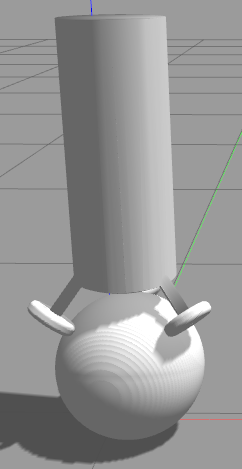
\includegraphics[width=5cm]{./Bilder/Markus/easy_model.png} }}%
	\qquad \qquad
	\subfloat[Simulation der freien R�der des Omnidirektionalen Rades.]{{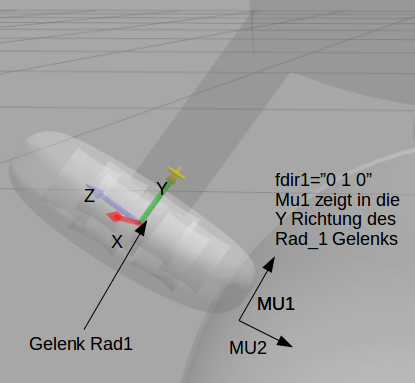
\includegraphics[width=6cm]{./Bilder/Markus/simulation_easy.png} }}%
	\caption{Die einfachste Simulations M�glichkeit eines Ballbots in Gazebo7.}%
	\label{fig:simple_simulation}%
\end{figure}

Die zweite M�glichkeit ist sehr viel aufwendiger, denn sie besteht darin, das echte Omnidirektionale Rad mit allen kleinen R�dern zu simulieren. Hierf�r muss zun�chst das Omnidirektionale Rad ohne die freilaufenden kleine Subr�der in die Gazebo Simulation geladen werden. Anschlie�end m�ssen die Subr�der mit richtiger Orientierung und Position ebenfalls in die Simulation geladen werden. Das Omnidirektionale Rad sowie ein einzelnes Subrad wurde hierf�r zun�chst in Solid Edge konstruiert und anschlie�end als .stl exportiert. Diese .stl Dateinen werden dann mittels einer .xml Datei in die Gazebo Simulation geladen. 

F�r unsere finale Ballbot Simulation haben wir die zweite M�glichkeit benutzt, denn sie ist der Realit�t sehr viel N�her als die Modellierung von unendlich vielen kleinen Subr�dern. Nachteilig bei der Simulation aller 30 Subr�der ist jedoch, der deutlich gr��ere Berechnungsaufwand, der in unserem Falle die Simulation auf einen RealTime Faktor von 0.2 verlangsamt hat. Das hei�t die Simulation lief f�nf mal langsamer als sie in Echtzeit laufen w�rde.

\section{Simulations Aufbau}
Dieses Kapitel zeigt zun�chst exemplarisch die Kommunikation zwischen ROS und Gazebo. Anschlie�end wird n�her auf die verwendeten Plugins eingeganen.
Zudem wird auf dynamische Eigenschaften der Simulation wie etwa die Steifigkeit einzelner Elemente eingeganen. Zum Schluss wird noch auf zwei Visualisierungsprogramme(RVIZ und PlotJuggler)  eingegangen. 

\subsection{Kommunikation zwischen ROS und Gazebo}
Die Simulation mittels Gazebo wurde komplett in ROS aufgebaut. Sie besteht aus mehreren Nodes (Teilprogrammen) die alle durch ein globales ROS launch file gestartet werden. Beim Ausf�hren der Simulation sind sehr viele Teilprogramme(Nodes) aktiv die untereinander �ber sogenannte Topics Nachrichten austauschen. 
\begin{figure}[htbp]%
	{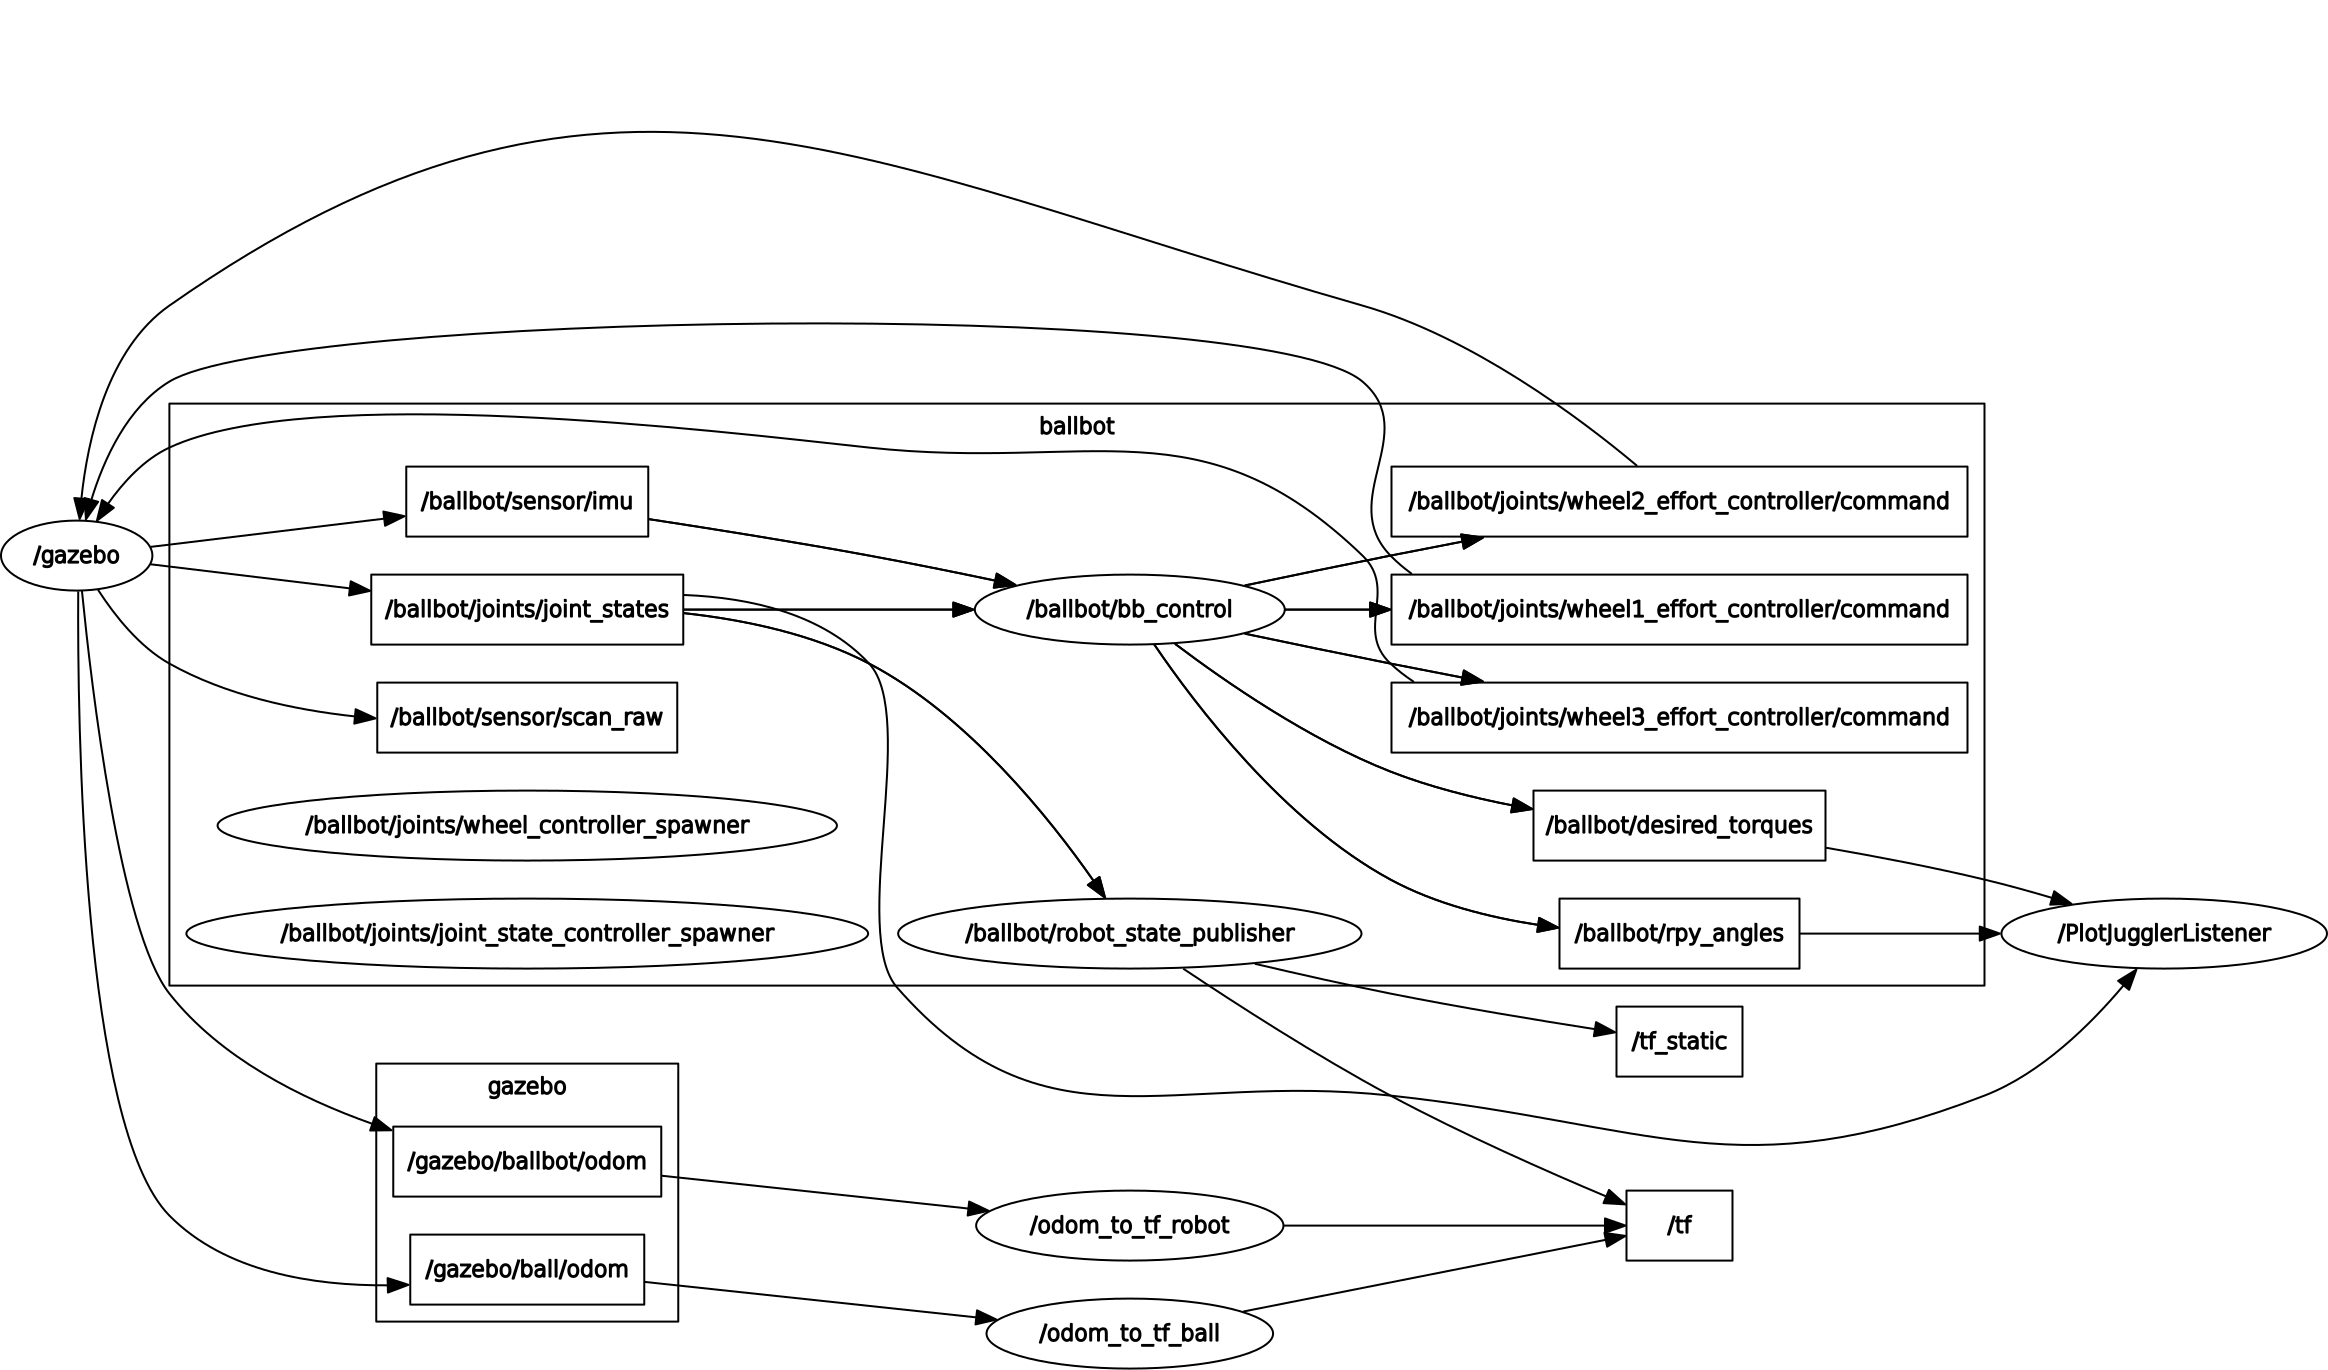
\includegraphics[scale=0.28]{./Bilder/Markus/rosgraph.png} }
	\caption{�bersicht aller Teilprogramme(Nodes) und deren Topics, die beim Starten der Simulation aktiv sind und Nachrichten austauschen. Hierbei sind die Nodes mit Ellipsen und die Topics mit Rechtecken gekennzeichnet. Das Bild wurde mit dem ROS Programm rqt\_graph erstellt.}
	\label{fig:ros_graph}
\end{figure}
Abbildung \ref{fig:ros_graph} zeigt den sogenannten ROS Graph der aktiven Nodes und deren Topics nach dem Starten des globalen ROS launch files. In der Mitte dieser Abbildung sieht man das den Node /ballbot/bb\_control des namspaces ballbot. Dies ist das Teilprogramm das die Regelung des simulierten Ballbots beinhaltet. Hierf�r liest(subscribt) es Nachrichten der Topics /ballbot/joints/joint\_states\footnote{Dieses Topic enth�lt eine Nachricht die die aktuellen Rad Drehmomente, Geschwindigkeiten [rad/sec] und deren absolute Positionen enth�lt. F�r die Regelung der Odometrie werden jedoch nur die Rad Drehgeschwindigkeiten verwendet. } und /ballbot/sensor/imu ein, berechnet damit die entsprechenden Drehmomente f�r die einzelnen R�der und ver�ffentlicht (published) die Nachrichten mit den berechneten Drehmomenten auf den Topics /ballbot/wheelx\_effort\_controller/command. Der Node /gazebo wiederum liest diese Drehmoment Befehle der einzelnen Omnidirektionalen R�der ein und dreht entsprechend in der sichtbaren Simulation die R�der. 

Es sei noch darauf hingewiesen, dass es m�glich ist Gazebo mit ROS zu synchronisieren. M�chte man zum Beispiel einen Regler implementieren, der eine sehr gro�e Update Frequenz (bzw. eine geringe Sample Time) aufwei�t, die Berechnung der Verst�rkungsfaktoren dieser Regelung jedoch l�nger dauert als die Sample Time, so muss die Regelung mit Gazebo synronisiert werden. Hierf�r gibt es die M�glichkeit, Gazebo pausiert zu starten und auch die ganze Zeit pausiert zu lassen. Ist nun die Berechnung der Regelung fertig, schickt man einen rosservice call an gazebo um die Simulation einen Schritt weiterlaufen zu lassen. Anschlie�end wird der n�chste Regelunswert berechnet. Bei dem simulierten Ballbot wurde eine Update Frequenz von 100Hz benutzt. Die Verst�rkungsfaktoren der 2D Regelung wurden jedoch mit mindestens 1000Hz berechnet. Daher musste Gazebo nicht mit dem entsprechendem ROS Node, der die Regelung darstellt (/ballbot\_controll) synronisiert werden. 


\subsection{Plugins der Simulation}
Die Sensoren des Ballbot's k�nnen in Gazebo durch Plugins simuliert werden. Abbildung \ref{fig:plugins_simulation} zeigt die simulierten Sensoren und deren Plugin Bibliotheken. Hierbei wurde die IMU mit einer update\_rate von 200Hz sowie mit einem Gau�schen Rausschen von 0.01 simuliert. Als Motoren Interface wurde das Joint Effort Interface verwendet, welches �ber das ros\_control Paket\footnote{Dieses Paket ist standardm��ig bei der ROS-Kinetic Version dabei. Weitere Informationen zu diesem Paket gibt es hier: http://wiki.ros.org/ros\_control .} zur Verf�gung steht. Die Motoren wurden dabei mit einem PID Regler simuliert. Dabei wurden die Verst�rkungsfaktoren zu P=100, I=0.01 und D=10 gew�hlt. F�r weitere Details zur Implementierung der Real-Sense Kamera sowie des LDS Laser Scanners sei auf den Programmcode\footnote{siehe: https://github.com/CesMak/bb/blob/master/src/ballbot/bb\_descrpition/urdf/bb\_double\_wheel.gazebo.xacro} verwiesen.

\begin{figure}[!htbp]%
	\centering
	{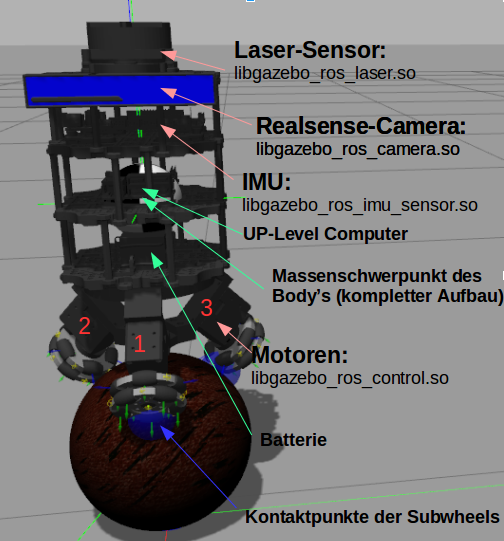
\includegraphics[scale=0.65]{./Bilder/Markus/simulation_plugins.png} }
	\caption{Der Simulierte Ballbot mit den simulierten Sensoren und deren Plugin Bibliotheken.}
	\label{fig:plugins_simulation}
\end{figure}
\subsection{Simulierte Dynamik-Eigenschaften}


%see here:http://ode.org/ode-latest-userguide.html
Nicht an dieser tabelle orientieren.
\begin{tabular}{l l l l}
	name(xacro)&description&value&sdf group\\
	mu1&is the Coulomb friction coefficient for the first friction direction&1.0&ode\\
	mu2& is the friction coefficient for the second friction direction (perpendicular to the first friction direction)&2.0&ode\\
	fdir1& 3-tuple specifying direction of mu1 in the collision local reference frame. fdir1 is the vector that defines the direction of mu1, which is the principal contact direction &0 0 0&ode\\
	kp&spring constant equivalents of a contact as a function of SurfaceParams::cfm and SurfaceParams::erp & &ode \\
	kd&spring damping constant equivalents of a contact as a function of SurfaceParams::cfm and SurfaceParams::erp.   & &ode \\
	cfm&Constraint Force Mixing parameter.& &ode \\
	erp&Error Reduction Parameter.& &ode \\
	min\_depth&Minimum depth before ERP takes effect.   & &ode \\
	max\_Vel& Maximum interpenetration error correction velocity.
	If set to 0, two objects interpenetrating each other will not be pushed apart.  & &ode \\
	slip1&Artificial contact slip in the primary friction direction  & &ode \\
	slip2&Artificial contact slip in the secondary friction dirction.& &ode \\
\end{tabular}

Ball so hart wie m�glich machen! in der simulation da wie in annahmen gesagt.

\subsection{Visualisierungsprogramme}
RVIZ, RQT-Multiplot


\chapter{Implementierung} \label{ch:Implementierung}
In diesem Kapitel wird zun�chst die eingesetzte Entwicklungsumgebung f�r die Programmierung des Regelgesetzes vorgestellt. Daraufhin wird die allgemeine Vorgehensweise der praktischen Umsetzung der Implementierung des Ballbot's erl�utert.   

\section{Entwicklungsumgebung}
Als Entwicklungsumgebung f�r den Zustandsregler des Ballbot's wird die ArduinoIDE \footnote{https://www.arduino.cc/en/Main/Software} eingesetzt, die in Abbildung \ref{fig:IDE} abgebildet ist. Die Hauptbestandteile dieser Entwicklungsumgebung umfassen einen Texteditor f�r das eigentliche Programm, eine Konsole f�r Fehler- und Kompilierungsmeldungen und einen seriellen Monitor f�r das Senden und Empfangen von Daten zwischen Computer und Board. Weiterhin eignet sich die Entwicklungsumgebung f�r den Einsatz, da ab der Version 1.6.4 das eingesetzte OpenCR-Board unterst�tzt wird. Allerdings muss die daf�r n�tige Bibliothek �ber den Boardverwalter nachinstalliert werden \cite{openCR} \cite{Arduino}.
\begin{figure}[htbp]
	\centering
		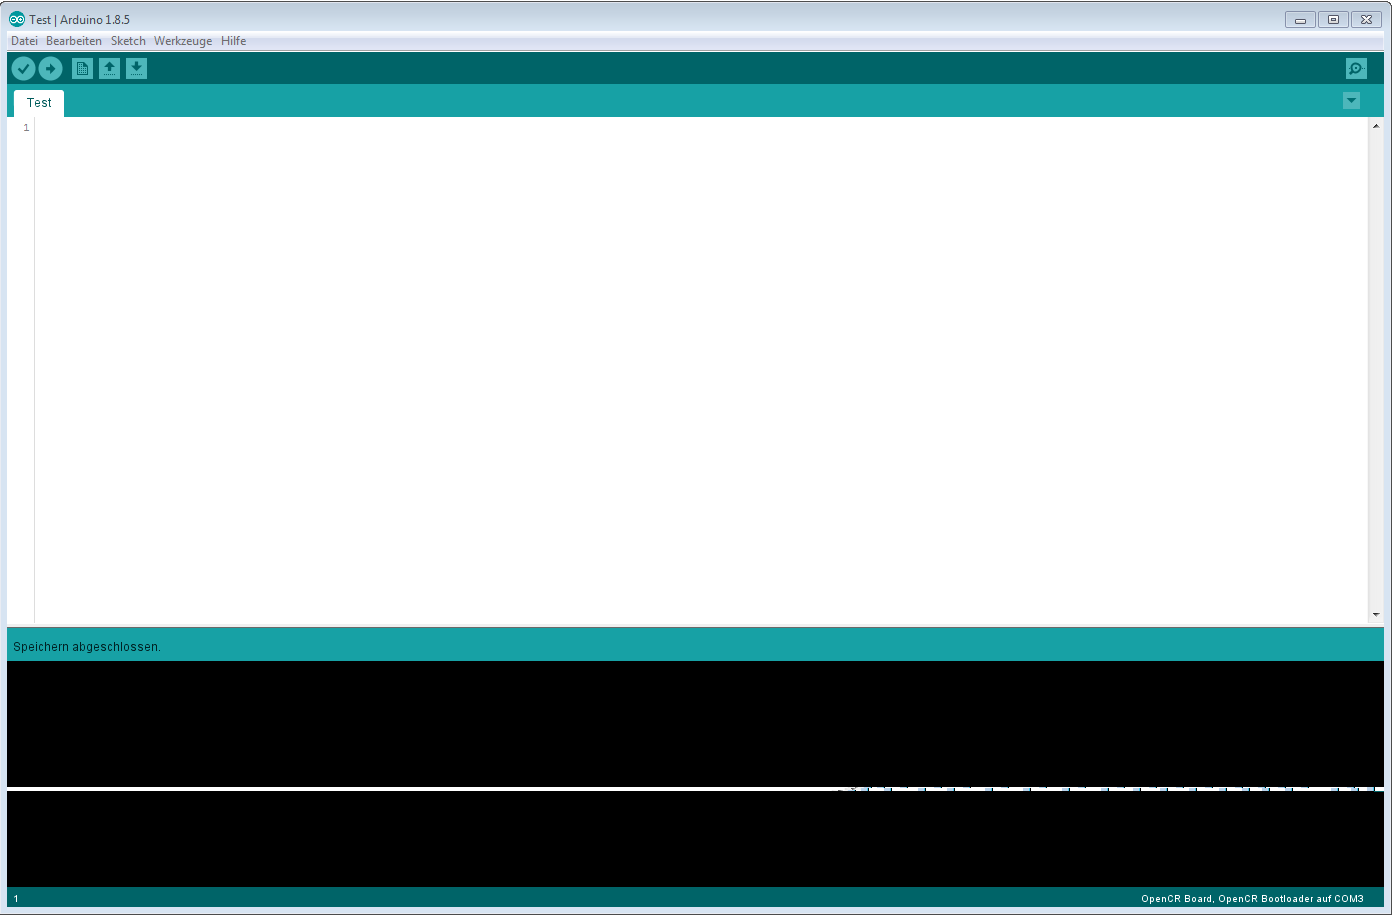
\includegraphics[width=0.70\textwidth]{Bilder/Florian/ArduinoIDE.PNG}
	\caption{Arduino Entwicklungsumgebung}
	\label{fig:IDE}
\end{figure}

Die Grundstruktur eines Programms, die im Listing \ref{lst:Programm} dargestellt ist, gliedert sich in zwei Bereiche. In der Setup-Funktionen, die nur einmal beim Start des Board ausgef�hrt wird, werden verschieden Initialisierungen f�r den sp�teren Programmablauf festgelegt. Bei der Loop-Funktion handelt es sich um das eigentliche Programm, die als endlose Schleife durchlaufen wird. Werden f�r das Programm noch weitere Funktionen bzw. Variablen ben�tigt, m�ssen diese am Anfang oder am Ende eines Programms definiert werden \cite{bruehl}.

\begin{lstlisting}[label=lst:Programm, style = C_colored_smallfont, caption=Grundstruktur eines Arduino-Programmes\cite{bruehl} ]
void setup()	{
		// Diese Funktion wird nur beim Starten 
		// des entsprechen Boards einmal ausgef�hrt
}

void loop()	{
		// Diese Funktion in einer endlosen Schleife 
		// durchlaufen
}
\end{lstlisting}
Um die �bersichtlichkeit zu steigern, k�nnen Funktionen und Klassendefinitionen in separaten Dateien ausgelagert werden und im Hauptprogramm eingebunden werden. 

\section{Hauptprogramm}
Die ben�tigten Daten f�r die Regelung werden nach dem EVA-Prinzip (Eingabe, Verarbeitung, Ausgabe) in einem Interrupt verarbeitet. Das bedeutet, dass das OpenCR-Board die ben�tigten Sensordaten des Gyroskops empf�ngt, entsprechend dem Regelgesetz aus Gl. \ref{eq:Regelgesetz} verarbeitet und die entsprechenden Stellgr��en an die einzelnen Motoren weiterleitet. Im Hauptprogramm sind folgende Bibliotheken aus der OpenCR-Bibliothek inkludiert worden:
\begin{itemize}
	\item IMU.h : Schnittstelle zur IMU.
	\item DynamixelSDK.h : Schnittstelle zu den Motoren.
\end{itemize}
Nachfolgend wird das Hauptprogramm n�her erl�utert.

\subsection{Initialisierung Komponenten}
F�r die Implementierung der Zustandsregelung m�ssen zun�chst die inertiale Messeinheit, die Motoren und der Hardware-Interrupt initialisiert werden. Hierzu wird die Setup-Funktion benutzt.

Bei der Initialisierung der IMU bzw. des gesamten Systems muss darauf geachtet werden, die richtige Update-Frequenz festzulegen bzw. zu �bergeben, damit das Gyroskop in m�glichst kurzen Zeitabst�nden aktualisierte Daten zur Verf�gung stellt und das System die aktuellen Stellgr��en berechnen kann.

Da der Ballbot seine Gleichgewichtslage durch das Aufbringen von entsprechenden Drehmomenten auf den Ball versucht zu halten, stellen diese  gleichzeitig die Stellgr��e des Systems dar. Daher m�ssen die drei Motoren zu Beginn auf die stromgeregelte Betriebsart konfiguriert und f�r den Einsatz freigeben werden. Die entsprechenden Adressen und Werte sind dem Datenblatt \cite{XM430} zu entnehmen.

Damit die Berechnung des Regelgesetzes nach Gl. \ref{eq:Regelgesetz} zu den Zeitpunkten der Aktualisierungsfrequenz durchgef�hrt werden kann, wird ein Hardware-Timer initialisiert, der als Interrupt arbeitet und in festgelegten Zeitabst�nden das Hauptprogramm des Mikrocontrollers unterbricht und einen Interrupt (Ausnahmeroutine) aufruft. Die auszuf�hrenden Funktionen der Routine sind f�r das Einlesen der Daten und die Berechnung der Stellgr��e zust�ndig. Die Abbildung \ref{fig:ISP} zeigt die Funktionsweise eines Interrupts.   

\begin{figure}[h!]
\centering
\scalebox{0.7}{
\begin{tikzpicture}[auto, thick ,node distance=0.5cm]
% Definition of blocks:
\usetikzlibrary{positioning,arrows,calc}
\tikzset{%
  block/.style    = {draw, thick, rectangle,  rounded corners, minimum height = 1.5em, minimum width = 8em, node distance = 1.5cm},
  %sum/.style      = {draw, circle, node distance = 1.5cm}, % Adder
	%join/.style			= {coordinate}, 
  input/.style    = {coordinate, node distance = 2cm} % Input
  %output/.style   = {coordinate} % Output
}

\draw
	node [block](Reset){Reset}
	node [block, below = of Reset] (Setup){setup()}
	node [input, below = of Setup] (Verzweigung) {}
	node [block, below = of Verzweigung] (Loop) {loop()}
	node [input, below = of Loop] (Temp1) {}
	node [input, right = of Temp1] (Temp2) {}
	node [input, right = of Verzweigung] (Temp3) {};
	
	
\draw[->](Reset) -- (Setup);	
\draw[-](Setup) -- (Verzweigung);
\draw[->](Verzweigung) -- (Loop);
\draw[-](Loop) -- (Temp1);
\draw[-](Temp1) -- (Temp2);
\draw[-](Temp2) -- (Temp3);
\draw[->](Temp3) -- (Verzweigung);


\draw
	node [input, right = of Reset] (Temp4) {}
	node [block, right = of Temp4] (Int) {Interrupt}
	node [block, below = of Int] (IMU){readIMU()}
	node [block, below = of IMU] (Regler){computeControler()}
	node [block, below = of Regler] (Torque) {computeTorques()}
	node [block, below = of Torque] (Return) {Return};

\draw[->](Int) -- (IMU);	
\draw[->](IMU) -- (Regler);
\draw[->](Regler) -- (Torque);
\draw[->](Torque) -- (Return);

\end{tikzpicture}
}
\caption{Links: Hauptprogramm. Rechts: Aufrufen und Abarbeiten der Serviceroutine}
\label{fig:ISP}
\end{figure}

\subsection{Einlesen der Sensordaten}
Der Zugriff auf die Winkel und Winkelgeschwindigkeiten wird durch das Einbinden der Bibliothek der inertialen Messeinheit hergestellt.

F�r die weitere Datenverarbeitung m�ssen die Winkel und Winkelgeschwindigkeiten, die in der Einheit Grad und Umdrehungen pro Minute angegeben sind, mit einer entsprechenden Funktion in die Einheit $\text{rad}$ und $\text{rad/s}$ konvertiert werden. Die Abbildung \ref{fig:Winkel} zeigt die Winkel $\vartheta_{x}$ und die entsprechenden Winkelgeschwindigkeiten $\dot{\vartheta}_{x}$. Aufgrund der h�heren �bersichtlichkeit sind diese in $\text{Grad}$ und $\text{Grad/s}$ angeben. Zudem ist zu erkennen, dass die Winkel mit einem Rauschen �berlagert sind. Zu beachten ist, dass die eingebundene IMU Bibliothek (IMU.h) intern einen MadgwickAHRS-Filter\footnote{F�r weitere Informationen siehe: \url{https://github.com/arduino-libraries/MadgwickAHRS}.} verwendet. Dieser wurde so �bernommen. Abbildung \ref{fig:Winkel} zeigt eine beispielhafte Ausgabe dieses Filters bei aufrechter Ruhelage des Roboters.

\begin{figure}[h!]
\centering
% This file was created by matlab2tikz.
%
%The latest updates can be retrieved from
%  http://www.mathworks.com/matlabcentral/fileexchange/22022-matlab2tikz-matlab2tikz
%where you can also make suggestions and rate matlab2tikz.
%
\definecolor{mycolor1}{rgb}{0.00000,0.44700,0.74100}%
%
\begin{tikzpicture}

\begin{axis}[%
width=0.951\figW,
height=0.419\figH,
at={(0\figW,0.581\figH)},
scale only axis,
scaled ticks=false,
xmin=0.015,
xmax=0.025,
xtick={0.015,0.0175,0.02,0.0225,0.025},
xticklabels={\empty},
ymin=-3,
ymax=1,
ytick={-3,-2,-1,0,1},
ylabel style={font=\color{white!15!black}},
ylabel={$\vartheta_{x}$ [$^{\circ}$]},
axis background/.style={fill=white},
xmajorgrids,
ymajorgrids
]
\addplot [color=mycolor1, line width=1.2pt, forget plot]
  table[row sep=crcr]{%
0.009443	-40.1\\
0.009542	-39.24\\
0.009641	-38.37\\
0.00974	-37.5\\
0.009839	-36.61\\
0.009938	-35.72\\
0.010037	-34.82\\
0.010136	-33.91\\
0.010235	-33\\
0.010334	-32.07\\
0.010433	-31.14\\
0.010532	-30.2\\
0.010631	-29.25\\
0.01073	-28.29\\
0.010829	-27.33\\
0.010928	-26.35\\
0.011027	-25.37\\
0.011126	-24.38\\
0.011225	-23.39\\
0.011324	-22.38\\
0.011423	-21.37\\
0.011522	-20.35\\
0.011621	-19.33\\
0.01172	-18.29\\
0.011819	-17.25\\
0.011918	-16.2\\
0.012017	-15.15\\
0.012116	-14.09\\
0.012215	-13.03\\
0.012314	-11.96\\
0.012413	-10.88\\
0.012512	-9.8\\
0.012611	-8.71\\
0.01271	-7.62\\
0.012809	-6.53\\
0.012908	-5.44\\
0.013007	-4.33\\
0.013106	-3.23\\
0.013205	-2.13\\
0.013304	-1.01\\
0.013403	-1.61\\
0.013502	-1.02\\
0.013601	-0.7\\
0.0137	-0.97\\
0.013799	-0.81\\
0.013898	-0.95\\
0.013997	-0.7\\
0.014096	-1.02\\
0.014195	-0.52\\
0.014294	-0.99\\
0.014393	-0.22\\
0.014492	-0.95\\
0.014591	-1.31\\
0.01469	-1.03\\
0.014789	-1.59\\
0.014888	-0.89\\
0.014987	-2.02\\
0.015086	-0.9\\
0.015185	-1.31\\
0.015284	-0.9\\
0.015383	-2.03\\
0.015482	-0.92\\
0.015581	-2.01\\
0.01568	-0.96\\
0.015779	-0.51\\
0.015878	-0.94\\
0.015977	0.12\\
0.016076	-0.98\\
0.016175	-0.54\\
0.016274	-0.97\\
0.016373	0.08\\
0.016472	-0.99\\
0.016571	-1.81\\
0.01667	-0.98\\
0.016769	-1.56\\
0.016868	-0.98\\
0.016967	-1.96\\
0.017066	-0.97\\
0.017165	-2.1\\
0.017264	-0.97\\
0.017363	-0.14\\
0.017462	-0.95\\
0.017561	-1.83\\
0.01766	-0.95\\
0.017759	-1.14\\
0.017858	-0.83\\
0.017957	-1.94\\
0.018056	-0.82\\
0.018155	-1.9\\
0.018254	-0.8\\
0.018353	-1.9\\
0.018452	-0.8\\
0.018551	-1.76\\
0.01865	-0.86\\
0.018749	-1.41\\
0.018848	-0.96\\
0.018947	-0.86\\
0.019046	-1.09\\
0.019145	-0.46\\
0.019244	-1.17\\
0.019343	-0.51\\
0.019442	-0.85\\
0.019541	-1.67\\
0.01964	-0.85\\
0.019739	-1.58\\
0.019838	-0.95\\
0.019937	-1.27\\
0.020036	-0.91\\
0.020135	-1.14\\
0.020234	-0.84\\
0.020333	-1.42\\
0.020432	-0.79\\
0.020531	-1.62\\
0.02063	-0.67\\
0.020729	-1.78\\
0.020828	-0.67\\
0.020927	-1.72\\
0.021026	-0.77\\
0.021125	-1.48\\
0.021224	-0.89\\
0.021323	-1.29\\
0.021422	-0.84\\
0.021521	-1.36\\
0.02162	-0.84\\
0.021719	-1\\
0.021818	-0.84\\
0.021917	-1.49\\
0.022016	-0.78\\
0.022115	-1.37\\
0.022214	-0.61\\
0.022313	-1.58\\
0.022412	-0.62\\
0.022511	-1.58\\
0.02261	-0.66\\
0.022709	-1.67\\
0.022808	-0.65\\
0.022907	-1.56\\
0.023006	-0.7\\
0.023105	-1.45\\
0.023204	-0.87\\
0.023303	-1.21\\
0.023402	-1.05\\
0.023501	-0.81\\
0.0236	-1.25\\
0.023699	-0.53\\
0.023798	-1.25\\
0.023897	-0.56\\
0.023996	-1.28\\
0.024095	-0.52\\
0.024194	-1.32\\
0.024293	-0.46\\
0.024392	-1.47\\
0.024491	-0.34\\
0.02459	-1.47\\
0.024689	-0.35\\
0.024788	-1.45\\
0.024887	-0.4\\
0.024986	-1.4\\
0.025085	-0.56\\
0.025184	-1.17\\
0.025283	-0.67\\
0.025382	-1.23\\
0.025481	-0.5\\
0.02558	-1.3\\
0.025679	-0.49\\
0.025778	-1.33\\
0.025877	-0.4\\
0.025976	-1.37\\
0.026075	-0.61\\
0.026174	-1.33\\
0.026273	-0.63\\
0.026372	-1.22\\
0.026471	-0.9\\
0.02657	-1.06\\
0.026669	-0.75\\
0.026768	-1.3\\
0.026867	-0.45\\
0.026966	-1.33\\
0.027065	-0.6\\
0.027164	-1.31\\
0.027263	-0.36\\
0.027362	-1.32\\
0.027461	-0.49\\
0.02756	-1.38\\
0.027659	-0.4\\
0.027758	-1.38\\
0.027857	-0.4\\
0.027956	-1.36\\
0.028055	-0.32\\
0.028154	-1.35\\
0.028253	-0.33\\
0.028352	-1.37\\
0.028451	-0.37\\
0.02855	-1.32\\
0.028649	-0.67\\
0.028748	-1.14\\
0.028847	-0.68\\
0.028946	-1.22\\
0.029045	-0.59\\
0.029144	-1.16\\
0.029243	-0.73\\
0.029342	-1.17\\
0.029441	-0.62\\
0.02954	-1.4\\
0.029639	-0.34\\
0.029738	-1.4\\
0.029837	-0.3\\
0.029936	-1.43\\
0.030035	-0.31\\
0.030134	-1.44\\
0.030233	-0.32\\
0.030332	-1.4\\
0.030431	-0.37\\
0.03053	-1.44\\
0.030629	-0.32\\
0.030728	-1.43\\
0.030827	-0.45\\
0.030926	-1.34\\
0.031025	-0.61\\
0.031124	-1.14\\
0.031223	-0.78\\
0.031322	-0.9\\
0.031421	-0.96\\
0.03152	-0.97\\
0.031619	-0.89\\
0.031718	-0.87\\
0.031817	-0.78\\
0.031916	-1.04\\
0.032015	-0.82\\
0.032114	-1.14\\
0.032213	-0.71\\
0.032312	-1.09\\
0.032411	-0.94\\
0.03251	-1.08\\
0.032609	-1.01\\
0.032708	-1.09\\
0.032807	-1.02\\
0.032906	-0.95\\
0.033005	-0.93\\
0.033104	-1.1\\
0.033203	-0.86\\
0.033302	-1.11\\
0.033401	-0.98\\
0.0335	-0.69\\
};
\end{axis}

\begin{axis}[%
width=0.951\figW,
height=0.419\figH,
at={(0\figW,0.1\figH)},
scale only axis,
scaled ticks=false,
xmin=0.015,
xmax=0.025,
xtick={0.015,0.0175,0.02,0.0225,0.025},
xticklabels={{0,015},{0,0175},{0,02},{0,0225},{0,025}},
xlabel style={font=\color{white!15!black}},
xlabel={t [$s$]},
ymin=-1,
ymax=1,
ytick={-0.5,0,0.5,1},
yticklabels={{-0,5},{0},{0,5},{1}},
ylabel style={font=\color{white!15!black}},
ylabel={$\dot{\vartheta_{x}}$ [$\frac{^{\circ}}{s}$]},
axis background/.style={fill=white},
xmajorgrids,
ymajorgrids
]
\addplot [color=mycolor1, line width=1.2pt, forget plot]
  table[row sep=crcr]{%
0.009443	0\\
0.009542	0\\
0.009641	0\\
0.00974	0\\
0.009839	0\\
0.009938	0\\
0.010037	0\\
0.010136	0\\
0.010235	0\\
0.010334	0\\
0.010433	0\\
0.010532	0\\
0.010631	0\\
0.01073	0\\
0.010829	0\\
0.010928	0\\
0.011027	0\\
0.011126	0\\
0.011225	0\\
0.011324	0\\
0.011423	0\\
0.011522	0\\
0.011621	0\\
0.01172	0\\
0.011819	0\\
0.011918	0\\
0.012017	0\\
0.012116	0\\
0.012215	0\\
0.012314	0\\
0.012413	0\\
0.012512	0\\
0.012611	0\\
0.01271	0\\
0.012809	0\\
0.012908	0\\
0.013007	0\\
0.013106	0\\
0.013205	0\\
0.013304	0\\
0.013403	0\\
0.013502	0\\
0.013601	0\\
0.0137	0\\
0.013799	0\\
0.013898	0\\
0.013997	0\\
0.014096	0\\
0.014195	0\\
0.014294	0\\
0.014393	0\\
0.014492	0\\
0.014591	0\\
0.01469	0\\
0.014789	0\\
0.014888	0\\
0.014987	0\\
0.015086	0\\
0.015185	0\\
0.015284	0\\
0.015383	0\\
0.015482	0\\
0.015581	0\\
0.01568	0\\
0.015779	0\\
0.015878	0\\
0.015977	0\\
0.016076	0\\
0.016175	0\\
0.016274	0\\
0.016373	0\\
0.016472	0\\
0.016571	0\\
0.01667	0\\
0.016769	0\\
0.016868	0\\
0.016967	0\\
0.017066	0\\
0.017165	0\\
0.017264	0\\
0.017363	0\\
0.017462	0\\
0.017561	0\\
0.01766	0\\
0.017759	0\\
0.017858	0\\
0.017957	0\\
0.018056	0\\
0.018155	0\\
0.018254	0\\
0.018353	0\\
0.018452	0\\
0.018551	0\\
0.01865	0\\
0.018749	0\\
0.018848	0\\
0.018947	0\\
0.019046	0\\
0.019145	0\\
0.019244	0\\
0.019343	0\\
0.019442	0\\
0.019541	0\\
0.01964	0\\
0.019739	0\\
0.019838	0\\
0.019937	0\\
0.020036	0\\
0.020135	0\\
0.020234	0\\
0.020333	0\\
0.020432	0\\
0.020531	0\\
0.02063	0\\
0.020729	0\\
0.020828	0\\
0.020927	0\\
0.021026	0\\
0.021125	0\\
0.021224	0\\
0.021323	0\\
0.021422	0\\
0.021521	0\\
0.02162	0\\
0.021719	0\\
0.021818	0\\
0.021917	0\\
0.022016	0\\
0.022115	0\\
0.022214	0\\
0.022313	0\\
0.022412	0\\
0.022511	0\\
0.02261	0\\
0.022709	0\\
0.022808	0\\
0.022907	0\\
0.023006	0\\
0.023105	0\\
0.023204	0\\
0.023303	0\\
0.023402	0\\
0.023501	0\\
0.0236	0\\
0.023699	0\\
0.023798	0\\
0.023897	0\\
0.023996	0\\
0.024095	0\\
0.024194	0\\
0.024293	0\\
0.024392	0\\
0.024491	0\\
0.02459	0\\
0.024689	0\\
0.024788	0\\
0.024887	0\\
0.024986	0\\
0.025085	0\\
0.025184	0\\
0.025283	0\\
0.025382	0\\
0.025481	0\\
0.02558	0\\
0.025679	0\\
0.025778	0\\
0.025877	0\\
0.025976	0\\
0.026075	0\\
0.026174	0\\
0.026273	0\\
0.026372	0\\
0.026471	0\\
0.02657	0\\
0.026669	0\\
0.026768	0\\
0.026867	0\\
0.026966	0\\
0.027065	0\\
0.027164	0\\
0.027263	0\\
0.027362	0\\
0.027461	0\\
0.02756	0\\
0.027659	0\\
0.027758	0\\
0.027857	0\\
0.027956	0\\
0.028055	0\\
0.028154	0\\
0.028253	0\\
0.028352	0\\
0.028451	0\\
0.02855	0\\
0.028649	0\\
0.028748	0\\
0.028847	0\\
0.028946	0\\
0.029045	0\\
0.029144	0\\
0.029243	0\\
0.029342	0\\
0.029441	0\\
0.02954	0\\
0.029639	0\\
0.029738	0\\
0.029837	0\\
0.029936	0\\
0.030035	0\\
0.030134	0\\
0.030233	0\\
0.030332	0\\
0.030431	0\\
0.03053	0\\
0.030629	0\\
0.030728	0\\
0.030827	0\\
0.030926	0\\
0.031025	0\\
0.031124	0\\
0.031223	0\\
0.031322	0\\
0.031421	0\\
0.03152	0\\
0.031619	0\\
0.031718	0\\
0.031817	0\\
0.031916	0\\
0.032015	0\\
0.032114	0\\
0.032213	0\\
0.032312	0\\
0.032411	0\\
0.03251	0\\
0.032609	0\\
0.032708	0\\
0.032807	0\\
0.032906	0\\
0.033005	0\\
0.033104	0\\
0.033203	0\\
0.033302	0\\
0.033401	0\\
0.0335	0\\
};
\end{axis}
\end{tikzpicture}%
\caption{Darstellung der Winkel $\vartheta_{x}$ und Winkelgeschwindigkeit $\dot{\vartheta}_{x}$}
\label{fig:Winkel}
\end{figure}

Um das Rauschen zu verringern, werden die letzten drei Sensorwerte der Winkel und Winkelgeschwindigkeiten gespeichert, aufsummiert und davon der Mittelwert gebildet. Das Ergebnis ist in Abbildung \ref{fig:Filter} zu sehen. 

\begin{figure}[h!]
	\centering
	% This file was created by matlab2tikz.
%
%The latest updates can be retrieved from
%  http://www.mathworks.com/matlabcentral/fileexchange/22022-matlab2tikz-matlab2tikz
%where you can also make suggestions and rate matlab2tikz.
%
\begin{tikzpicture}

\begin{axis}[%
width=0.951\figW,
height=\figH,
at={(0\figW,0\figH)},
scale only axis,
xmin=31,
xmax=33,
xtick={31,31.5,32,32.5,33},
xticklabels={{31},{31,5},{32},{32,5},{33}},
xlabel style={font=\color{white!15!black}},
xlabel={t in [s]},
ymin=-1,
ymax=0,
ytick={-1,-0.75,-0.5,-0.25,0},
yticklabels={{-1},{-0,75},{-0,5},{-0,25},{0}},
ylabel style={font=\color{white!15!black}},
ylabel={$\vartheta_{x}$ [$^{\circ}$]},
axis background/.style={fill=white},
xmajorgrids,
ymajorgrids,
legend style={legend cell align=left, align=left, draw=white!15!black}
]
\addplot [color=blue, line width=1.2pt]
  table[row sep=crcr]{%
30	-0.24\\
30.03	-0.49\\
30.06	-0.37\\
30.1	-0.56\\
30.13	-0.19\\
30.16	-0.56\\
30.2	-0.26\\
30.23	-0.42\\
30.26	-0.41\\
30.29	-0.47\\
30.33	-0.72\\
30.36	-0.4\\
30.39	-0.14\\
30.43	-0.4\\
30.46	-0.73\\
30.49	-0.43\\
30.53	-0.76\\
30.56	-0.51\\
30.59	-0.22\\
30.62	-0.52\\
30.66	-0.77\\
30.69	-0.45\\
30.72	-0.14\\
30.76	-0.49\\
30.79	-0.86\\
30.82	-0.57\\
30.86	-0.22\\
30.89	-0.44\\
30.92	-0.47\\
30.95	-0.82\\
30.99	-0.44\\
31.02	-0.07\\
31.05	-0.42\\
31.09	-0.34\\
31.12	-0.54\\
31.15	-0.17\\
31.19	-0.45\\
31.22	-0.28\\
31.25	-0.66\\
31.28	-0.46\\
31.32	-0.14\\
31.35	-0.51\\
31.38	-0.58\\
31.42	-0.47\\
31.45	-0.4\\
31.48	-0.46\\
31.52	-0.25\\
31.55	-0.45\\
31.58	-0.71\\
31.61	-0.46\\
31.65	-0.83\\
31.68	-0.5\\
31.71	-0.16\\
31.75	-0.51\\
31.78	-0.59\\
31.81	-0.54\\
31.85	-0.18\\
31.88	-0.54\\
31.91	-0.37\\
31.94	-0.42\\
31.98	-0.73\\
32.01	-0.39\\
32.04	-0.61\\
32.08	-0.36\\
32.11	-0.5\\
32.14	-0.47\\
32.18	-0.1\\
32.21	-0.45\\
32.24	-0.48\\
32.27	-0.8\\
32.31	-0.44\\
32.34	-0.47\\
32.37	-0.37\\
32.41	-0.39\\
32.44	-0.51\\
32.47	-0.25\\
32.51	-0.56\\
32.54	-0.19\\
32.57	-0.56\\
32.6	-0.32\\
32.64	-0.4\\
32.67	-0.48\\
32.7	-0.48\\
32.74	-0.41\\
32.77	-0.78\\
32.8	-0.46\\
32.84	-0.79\\
32.87	-0.5\\
32.9	-0.24\\
32.93	-0.53\\
32.97	-0.26\\
33	-0.44\\
33.03	-0.75\\
33.07	-0.39\\
33.1	-0.72\\
33.13	-0.39\\
33.17	-0.49\\
33.2	-0.5\\
33.23	-0.23\\
33.26	-0.37\\
33.3	-0.67\\
33.33	-0.4\\
33.36	-0.77\\
33.4	-0.39\\
33.43	-0.77\\
33.46	-0.4\\
33.5	-0.73\\
33.53	-0.41\\
33.56	-0.79\\
33.59	-0.42\\
33.63	-0.67\\
33.66	-0.48\\
33.69	-0.2\\
33.73	-0.58\\
33.76	-0.35\\
33.79	-0.59\\
33.83	-0.36\\
33.86	-0.62\\
33.89	-0.24\\
33.92	-0.54\\
33.96	-0.35\\
33.99	-0.4\\
34.02	-0.49\\
34.06	-0.39\\
34.09	-0.42\\
34.12	-0.78\\
34.16	-0.41\\
34.19	-0.04\\
34.22	-0.4\\
34.25	-0.54\\
34.29	-0.51\\
34.32	-0.45\\
34.35	-0.53\\
34.39	-0.18\\
34.42	-0.52\\
34.45	-0.51\\
34.49	-0.14\\
34.52	-0.52\\
34.55	-0.41\\
34.58	-0.5\\
34.62	-0.54\\
34.65	-0.47\\
34.68	-0.13\\
34.72	-0.47\\
34.75	-0.56\\
34.78	-0.3\\
34.82	-0.42\\
34.85	-0.38\\
34.88	-0.75\\
34.91	-0.38\\
34.95	-0.58\\
34.98	-0.48\\
35.01	-0.6\\
};
\addlegendentry{ungefiltert}

\addplot [color=red, dashdotted, line width=2.0pt]
  table[row sep=crcr]{%
30	-0.41\\
30.03	-0.34\\
30.06	-0.37\\
30.1	-0.47\\
30.13	-0.37\\
30.16	-0.44\\
30.2	-0.34\\
30.23	-0.41\\
30.26	-0.37\\
30.29	-0.43\\
30.33	-0.53\\
30.36	-0.53\\
30.39	-0.42\\
30.43	-0.31\\
30.46	-0.42\\
30.49	-0.52\\
30.53	-0.64\\
30.56	-0.57\\
30.59	-0.5\\
30.62	-0.42\\
30.66	-0.5\\
30.69	-0.58\\
30.72	-0.45\\
30.76	-0.36\\
30.79	-0.49\\
30.82	-0.64\\
30.86	-0.55\\
30.89	-0.41\\
30.92	-0.38\\
30.95	-0.58\\
30.99	-0.58\\
31.02	-0.44\\
31.05	-0.31\\
31.09	-0.28\\
31.12	-0.43\\
31.15	-0.35\\
31.19	-0.39\\
31.22	-0.3\\
31.25	-0.46\\
31.28	-0.47\\
31.32	-0.42\\
31.35	-0.37\\
31.38	-0.41\\
31.42	-0.52\\
31.45	-0.48\\
31.48	-0.44\\
31.52	-0.37\\
31.55	-0.39\\
31.58	-0.47\\
31.61	-0.54\\
31.65	-0.67\\
31.68	-0.6\\
31.71	-0.5\\
31.75	-0.39\\
31.78	-0.42\\
31.81	-0.54\\
31.85	-0.44\\
31.88	-0.42\\
31.91	-0.36\\
31.94	-0.44\\
31.98	-0.51\\
32.01	-0.52\\
32.04	-0.58\\
32.08	-0.46\\
32.11	-0.49\\
32.14	-0.45\\
32.18	-0.36\\
32.21	-0.34\\
32.24	-0.34\\
32.27	-0.58\\
32.31	-0.58\\
32.34	-0.57\\
32.37	-0.43\\
32.41	-0.41\\
32.44	-0.43\\
32.47	-0.38\\
32.51	-0.44\\
32.54	-0.33\\
32.57	-0.44\\
32.6	-0.36\\
32.64	-0.43\\
32.67	-0.4\\
32.7	-0.45\\
32.74	-0.46\\
32.77	-0.56\\
32.8	-0.55\\
32.84	-0.68\\
32.87	-0.59\\
32.9	-0.51\\
32.93	-0.43\\
32.97	-0.35\\
33	-0.41\\
33.03	-0.48\\
33.07	-0.52\\
33.1	-0.62\\
33.13	-0.5\\
33.17	-0.53\\
33.2	-0.46\\
33.23	-0.41\\
33.26	-0.37\\
33.3	-0.42\\
33.33	-0.48\\
33.36	-0.61\\
33.4	-0.52\\
33.43	-0.64\\
33.46	-0.52\\
33.5	-0.63\\
33.53	-0.51\\
33.56	-0.65\\
33.59	-0.54\\
33.63	-0.63\\
33.66	-0.53\\
33.69	-0.45\\
33.73	-0.42\\
33.76	-0.38\\
33.79	-0.51\\
33.83	-0.43\\
33.86	-0.52\\
33.89	-0.41\\
33.92	-0.47\\
33.96	-0.38\\
33.99	-0.43\\
34.02	-0.41\\
34.06	-0.43\\
34.09	-0.43\\
34.12	-0.53\\
34.16	-0.54\\
34.19	-0.41\\
34.22	-0.28\\
34.25	-0.32\\
34.29	-0.48\\
34.32	-0.5\\
34.35	-0.5\\
34.39	-0.39\\
34.42	-0.41\\
34.45	-0.4\\
34.49	-0.39\\
34.52	-0.39\\
34.55	-0.36\\
34.58	-0.48\\
34.62	-0.48\\
34.65	-0.5\\
34.68	-0.38\\
34.72	-0.36\\
34.75	-0.38\\
34.78	-0.44\\
34.82	-0.42\\
34.85	-0.37\\
34.88	-0.52\\
34.91	-0.5\\
34.95	-0.57\\
34.98	-0.48\\
35.01	-0.55\\
};
\addlegendentry{gefiltert}

\end{axis}
\end{tikzpicture}%
	\caption{Beispielhafter Vergleich zwischen ungefilterten(blau) und gefilterten Messwinkel}
	\label{fig:Filter}
\end{figure}


\subsection{Verarbeitung Sensordaten}
Mit den ausgelesenen Sensordaten k�nnen die einzelnen virtuellen Drehmomente f�r die entsprechenden Ebenen berechnet werden. Das virtuelle Drehmoment f�r die $xy$-Ebene wird auf Null gesetzt, da diese Orientierung um die $z$-Achse f�r die Regelung nicht ber�cksichtigt wird.\newline
Mit den berechneten, virtuellen Drehmomenten kann auf die realen Drehmomente f�r die einzelnen Motoren nach Gl. \ref{eq:realeDrehmomente} umgerechnet werden. Damit der Zeitaufwand f�r Berechnung m�glichst klein ist, werden konstante, mathematische Operationen durch feste Zahlenwerte festgelegt. Das Listing \ref{lst:Defines} zeigt einen Ausschnitt dieser Definitionen. 

\begin{lstlisting}[label=lst:Defines, style = C_colored_smallfont, caption=Zuweisen fester Zahlenwerte f�r eine k�rzerer Berechnungsdauer]
#define ALPHA                           PI/4
#define BETA                            0
#define COS_ALPHA                       0.70710678118      
#define SIN_ALPHA                       0.70710678118 
#define SIN_BETA                        0.0
#define COS_BETA                        1.0
#define SQRT3                           1.73205080757
\end{lstlisting}

 
\subsection{Ausgabe Drehmomente}
Das OpenCR-Board kommuniziert mit den Motoren �ber die RS485-Schnittstelle. Daher m�ssen f�r die �bertragung die berechneten Drehmomente in �quivalente, dimensionslose Einheiten (Unit) umgerechnet werden.
Diese Umrechnungskonstanten sind experimentell im Kapitel \ref{sec:Motoren} bestimmt worden. 

Da in der Modellbildung die Reibung zwischen Motor und Ball vernachl�ssigt wurde, muss ein Offset der Drehmomente eingestellt werden, damit diese Reibung �berwunden werden kann \cite{ETHZ}.

\section{Auswertung}
Nach der Implementierung des Mikrocontroller-Programms wurde die Regelung, wie in Kapitel \ref{ch:Modellierung} beschrieben, am realen Ballbot getestet. Abbildung \ref{fig:ballbot_real} zeigt den Aufbau des Ballbots wie er auf dem Ball balanciert. F�r dieses balancierende Experiment wurden zus�tzlich die Winkel der IMU und die realen Drehmomente der Motoren aufgenommen. Abbildung \ref{fig:Momente_bal} zeigt, dass die Motorendrehmomente nach Ausregelung einer kleinen Anfangsst�rung\footnote{Die kleine Anfangsst�rung hat die Ursache, dass der Ballbot nicht perfekt vertikal auf dem Ball platziert wurde.}, zwischen $-0.7$\,Nm und $+0.7$\,Nm pendeln. Anhand der Winkel $\vartheta_x, \vartheta_y$ in Abbildung \ref{fig:Winkel_bal} sieht man, dass eine Anfangsauslenkung von $5^\circ$ ausgeregelt werden konnte. Balanciert der Roboter so wurde ein maximaler Winkel von $|\vartheta|_{max} \ 2^\circ$ nicht �berschritten. Die 
Standardabweichungen der Auslenkungswinkel des balancierenden Roboters lagen bei: $\sigma_{\vartheta_x}=1.19^\circ$ und $\sigma_{\vartheta_y}=1.11^\circ$. Die Standardabweichungen der Motoren lagen bei $\sigma_{T1}=0.24$\,Nm $\sigma_{T2}=0.23$\,Nm und $\sigma_{T3}=0.28$\,Nm. Insgesamt hat sich ein stabiles Verhalten ergeben.

\begin{figure}[h!]
	\centering
	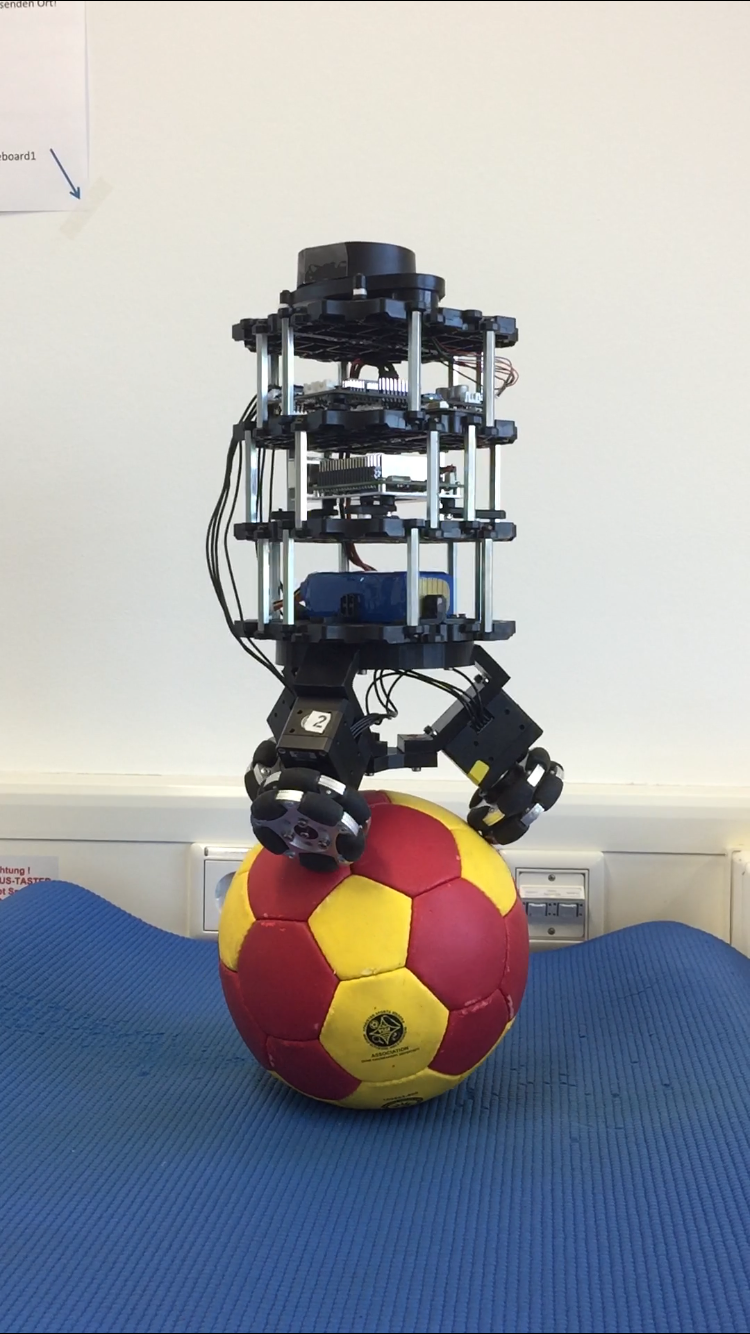
\includegraphics[scale=0.2]{./Bilder/Florian/ballbot_real.png}
	\caption{Aufbau des realen Ballbots.}
	\label{fig:ballbot_real}
\end{figure}

Das Regelverhalten weist jedoch Grenzen auf. Weitere Optimierungen f�r ein robusteres Regelverhalten sind:

\begin{itemize}\itemsep-0.5\parsep
	\item \text{Ball:}\
	\ Es konnte zwar ein Ball gefunden werden, der einen guten Kompromiss(vgl. Kapitel \ref{sec:ball}) zwischen den gew�nschten Eigenschaften bietet, allerdings k�nnte dieser Kompromiss noch weiter verbessert werden. So kann zum Beispiel mit einer ma�genauen Aluminiumhohlkugel mit Gummibeschichtung die n�tige notwendige Steifigkeit und den Reibwert bereitstellen.
	
	\item \text{Filterung des Messdaten:}\
	\ Auch die Filterung hat einen gro�en Einfluss auf die Regelg�te. Im bestehenden Ballbot ist ein einfacher Mittelwertfilter verwendet worden. Dadurch konnte das Rauschen in einigen F�llen schon um den Faktor 2 reduziert werden, jedoch ist das Rauschen weiterhin im Regelverhalten zu sp�ren. Eine Verbesserung in diesem Verhalten k�nnte durch ein besseres Filter beispielsweise ein Kalmanfilter erzielt werden. Dies h�tte zudem den Vorteil, dass kein Zeitverzug entstehen w�rde.
	
	\item \text{Modellierung:}\
	\ Auch bei der Modellierung des Ballbots sind Vereinfachungen getroffen worden. Es hat sich gezeigt, dass die Vereinfachung zul�ssig sind und eine zweckm��ige Regelung implementiert werden kann. Allerdings werden damit Verkopplungen zwischen der xz- und yz-Ebene vernachl�ssigt. Diese sind zwar relativ klein, bei Ber�cksichtigung dieser Verkopplungen k�nnte jedoch sicherlich ein noch besseres Regelverhalten erzielt werden. Dies k�nnte durch eine 3D-Regelung erzielen werden. 
	
	\item \text{Motoren:}\
	\ Die im Projekt verwendeten Motoren weisen Drehzahlbegrenzungen auf. Sowohl Experimente als auch Simulation konnten zeigen, dass das System nicht wie vorgesehen stabilisiert werden kann. Durch die Verwendung anderer Motoren, die eine h�here Drehzahlbegrenzung aufweisen kann dieser Effekt umgangen werden.
\end{itemize}

\begin{figure}[h!]
	\centering
	% This file was created by matlab2tikz.
%
%The latest updates can be retrieved from
%  http://www.mathworks.com/matlabcentral/fileexchange/22022-matlab2tikz-matlab2tikz
%where you can also make suggestions and rate matlab2tikz.
%
\definecolor{mycolor1}{rgb}{0.00000,0.44700,0.74100}%
\definecolor{mycolor2}{rgb}{0.85000,0.32500,0.09800}%
%
\begin{tikzpicture}

\begin{axis}[%
width=0.951\figW,
height=\figH,
at={(0\figW,0\figH)},
scale only axis,
xmin=0,
xmax=46.67,
xtick={0,5,10,15,20,25,30,35,40,45},
xlabel style={font=\color{white!15!black}},
xlabel={t [$s$]},
ymin=-10,
ymax=5,
ytick={-10,-5,0,5},
ylabel style={font=\color{white!15!black}},
ylabel={$\vartheta_{x,y}$ [$^{\circ}$]},
axis background/.style={fill=white},
xmajorgrids,
ymajorgrids,
legend style={legend cell align=left, align=left, draw=white!15!black}
]
\addplot [color=mycolor1, line width=1.2pt, forget plot]
  table[row sep=crcr]{%
0	0.67\\
0.0100000000000051	0.59\\
0.0200000000000031	0.5\\
0.0300000000000011	0.4\\
0.0300000000000011	0.29\\
0.0399999999999991	0.16\\
0.0500000000000043	0.04\\
0.0500000000000043	-0.08\\
0.0600000000000023	-0.19\\
0.0700000000000003	-0.29\\
0.0700000000000003	-0.39\\
0.0799999999999983	-0.49\\
0.0900000000000034	-0.55\\
0.0900000000000034	-0.55\\
0.100000000000001	-0.56\\
0.109999999999999	-0.6\\
0.120000000000005	-0.65\\
0.120000000000005	-0.66\\
0.130000000000003	-0.62\\
0.140000000000001	-0.58\\
0.140000000000001	-0.55\\
0.149999999999999	-0.52\\
0.160000000000004	-0.48\\
0.160000000000004	-0.46\\
0.170000000000002	-0.46\\
0.18	-0.47\\
0.18	-0.51\\
0.190000000000005	-0.58\\
0.200000000000003	-0.66\\
0.210000000000001	-0.76\\
0.210000000000001	-0.88\\
0.219999999999999	-1.02\\
0.230000000000004	-1.16\\
0.230000000000004	-1.32\\
0.240000000000002	-1.5\\
0.25	-1.68\\
0.25	-1.87\\
0.260000000000005	-2.07\\
0.270000000000003	-2.27\\
0.280000000000001	-2.47\\
0.280000000000001	-2.69\\
0.289999999999999	-2.9\\
0.300000000000004	-3.11\\
0.300000000000004	-3.32\\
0.310000000000002	-3.56\\
0.32	-3.8\\
0.32	-4.03\\
0.329999999999998	-4.27\\
0.340000000000003	-4.52\\
0.340000000000003	-4.78\\
0.350000000000001	-5.03\\
0.359999999999999	-5.28\\
0.370000000000005	-5.5\\
0.370000000000005	-5.7\\
0.380000000000003	-5.86\\
0.390000000000001	-6\\
0.390000000000001	-6.11\\
0.399999999999999	-6.19\\
0.410000000000004	-6.24\\
0.410000000000004	-6.25\\
0.420000000000002	-6.23\\
0.43	-6.17\\
0.440000000000005	-6.08\\
0.440000000000005	-5.97\\
0.450000000000003	-5.84\\
0.460000000000001	-5.69\\
0.460000000000001	-5.51\\
0.469999999999999	-5.33\\
0.480000000000004	-5.12\\
0.480000000000004	-4.87\\
0.490000000000002	-4.63\\
0.5	-4.37\\
0.510000000000005	-4.06\\
0.510000000000005	-3.76\\
0.520000000000003	-3.46\\
0.530000000000001	-3.17\\
0.530000000000001	-2.86\\
0.539999999999999	-2.54\\
0.550000000000004	-2.22\\
0.550000000000004	-1.88\\
0.560000000000002	-1.54\\
0.57	-1.2\\
0.57	-0.86\\
0.579999999999998	-0.54\\
0.590000000000003	-0.24\\
0.600000000000001	0.05\\
0.600000000000001	0.3\\
0.609999999999999	0.53\\
0.620000000000005	0.74\\
0.620000000000005	0.92\\
0.630000000000003	1.04\\
0.640000000000001	1.17\\
0.640000000000001	1.31\\
0.649999999999999	1.43\\
0.660000000000004	1.54\\
0.670000000000002	1.62\\
0.670000000000002	1.67\\
0.68	1.69\\
0.690000000000005	1.69\\
0.690000000000005	1.68\\
0.700000000000003	1.66\\
0.710000000000001	1.63\\
0.710000000000001	1.6\\
0.719999999999999	1.58\\
0.730000000000004	1.57\\
0.740000000000002	1.55\\
0.740000000000002	1.51\\
0.75	1.46\\
0.760000000000005	1.39\\
0.760000000000005	1.32\\
0.770000000000003	1.24\\
0.780000000000001	1.17\\
0.780000000000001	1.09\\
0.789999999999999	1.02\\
0.800000000000004	0.96\\
0.810000000000002	0.91\\
0.810000000000002	0.86\\
0.82	0.82\\
0.829999999999998	0.76\\
0.829999999999998	0.69\\
0.840000000000003	0.6\\
0.850000000000001	0.49\\
0.850000000000001	0.37\\
0.859999999999999	0.24\\
0.870000000000005	0.1\\
0.880000000000003	-0.03\\
0.880000000000003	-0.16\\
0.890000000000001	-0.28\\
0.899999999999999	-0.4\\
0.899999999999999	-0.5\\
0.910000000000004	-0.59\\
0.920000000000002	-0.69\\
0.920000000000002	-0.82\\
0.93	-0.97\\
0.940000000000005	-1.13\\
0.950000000000003	-1.28\\
0.950000000000003	-1.44\\
0.960000000000001	-1.59\\
0.969999999999999	-1.74\\
0.969999999999999	-1.86\\
0.980000000000004	-1.97\\
0.990000000000002	-2.1\\
0.990000000000002	-2.24\\
1	-2.38\\
1.01000000000001	-2.51\\
1.01000000000001	-2.66\\
1.02	-2.81\\
1.03	-2.95\\
1.04	-3.08\\
1.04	-3.2\\
1.05	-3.3\\
1.06	-3.38\\
1.06	-3.46\\
1.07	-3.53\\
1.08	-3.61\\
1.08	-3.68\\
1.09	-3.77\\
1.1	-3.87\\
1.11	-3.97\\
1.11	-4.07\\
1.12	-4.19\\
1.13	-4.31\\
1.13	-4.45\\
1.14	-4.59\\
1.15	-4.74\\
1.15	-4.93\\
1.16	-5.14\\
1.17	-5.39\\
1.18	-5.64\\
1.18	-5.89\\
1.19	-6.13\\
1.2	-6.37\\
1.2	-6.59\\
1.21	-6.8\\
1.22	-7\\
1.22	-7.18\\
1.23	-7.36\\
1.24	-7.53\\
1.24	-7.68\\
1.25	-7.83\\
1.26000000000001	-7.95\\
1.27	-8.06\\
1.27	-8.16\\
1.28	-8.22\\
1.29	-8.21\\
1.29	-8.18\\
1.3	-8.18\\
1.31	-8.17\\
1.31	-8.16\\
1.32	-8.13\\
1.33	-8.08\\
1.34	-8\\
1.34	-7.89\\
1.35	-7.74\\
1.36	-7.56\\
1.36	-7.37\\
1.37	-7.18\\
1.38	-6.98\\
1.38	-6.79\\
1.39	-6.6\\
1.4	-6.43\\
1.41	-6.25\\
1.41	-6.08\\
1.42	-5.91\\
1.43	-5.75\\
1.43	-5.59\\
1.44	-5.43\\
1.45	-5.28\\
1.45	-5.14\\
1.46	-5\\
1.47	-4.87\\
1.48	-4.75\\
1.48	-4.64\\
1.49	-4.54\\
1.5	-4.44\\
1.5	-4.36\\
1.51000000000001	-4.28\\
1.52	-4.21\\
1.52	-4.18\\
1.53	-4.15\\
1.54	-4.12\\
1.54	-4.11\\
1.55	-4.09\\
1.56	-4.07\\
1.57	-4.05\\
1.57	-4.02\\
1.58	-4\\
1.59	-3.97\\
1.59	-3.95\\
1.6	-3.91\\
1.61	-3.88\\
1.61	-3.85\\
1.62	-3.81\\
1.63	-3.8\\
1.64	-3.8\\
1.64	-3.83\\
1.65	-3.8\\
1.66	-3.7\\
1.66	-3.59\\
1.67	-3.48\\
1.68	-3.38\\
1.68	-3.29\\
1.69	-3.22\\
1.7	-3.16\\
1.71	-3.1\\
1.71	-3.06\\
1.72	-3.03\\
1.73	-3.01\\
1.73	-2.98\\
1.74	-2.93\\
1.75	-2.87\\
1.75	-2.79\\
1.76000000000001	-2.68\\
1.77	-2.59\\
1.78	-2.52\\
1.78	-2.45\\
1.79	-2.37\\
1.8	-2.28\\
1.8	-2.17\\
1.81	-2.05\\
1.82	-1.92\\
1.82	-1.79\\
1.83	-1.74\\
1.84	-1.64\\
1.84	-1.46\\
1.85	-1.2\\
1.86	-0.91\\
1.87	-0.64\\
1.87	-0.37\\
1.88	-0.09\\
1.89	0.21\\
1.89	0.51\\
1.9	0.8\\
1.91	1.09\\
1.91	1.37\\
1.92	1.66\\
1.93	1.94\\
1.94	2.21\\
1.94	2.48\\
1.95	2.73\\
1.96	2.97\\
1.96	3.2\\
1.97	3.43\\
1.98	3.65\\
1.98	3.85\\
1.99	4.02\\
2	4.18\\
2	4.26\\
2.01000000000001	4.17\\
2.02	3.99\\
2.03	3.78\\
2.03	3.57\\
2.04	3.38\\
2.05	3.18\\
2.05	2.95\\
2.06	2.7\\
2.07	2.45\\
2.07	2.21\\
2.08	1.98\\
2.09	1.76\\
2.1	1.54\\
2.1	1.35\\
2.11	1.17\\
2.12	1.04\\
2.12	0.9\\
2.13	0.7\\
2.14	0.48\\
2.14	0.26\\
2.15	0.05\\
2.16	-0.17\\
2.16	-0.4\\
2.17	-0.63\\
2.18	-0.86\\
2.19	-1.05\\
2.19	-1.17\\
2.2	-1.21\\
2.21	-1.19\\
2.21	-1.1\\
2.22	-0.94\\
2.23	-0.74\\
2.23	-0.49\\
2.24	-0.18\\
2.25	0.12\\
2.25	0.28\\
2.26000000000001	0.31\\
2.27	0.28\\
2.28	0.22\\
2.28	0.18\\
2.29	0.16\\
2.3	0.16\\
2.3	0.21\\
2.31	0.31\\
2.32	0.44\\
2.32	0.53\\
2.33	0.6\\
2.34	0.64\\
2.34	0.65\\
2.35	0.61\\
2.36	0.52\\
2.37	0.33\\
2.37	0.06\\
2.38	-0.25\\
2.39	-0.55\\
2.39	-0.82\\
2.4	-1\\
2.41	-1.08\\
2.41	-1.07\\
2.42	-1.02\\
2.43	-1.02\\
2.44	-1.02\\
2.44	-0.99\\
2.45	-0.95\\
2.46	-0.9\\
2.46	-0.85\\
2.47	-0.8\\
2.48	-0.75\\
2.48	-0.67\\
2.49	-0.65\\
2.5	-0.65\\
2.5	-0.63\\
2.51000000000001	-0.61\\
2.52	-0.62\\
2.53	-0.67\\
2.53	-0.75\\
2.54	-0.84\\
2.55	-0.95\\
2.55	-1.03\\
2.56	-1.08\\
2.57	-1.08\\
2.57	-1.06\\
2.58	-1.01\\
2.59	-0.95\\
2.59	-0.88\\
2.6	-0.77\\
2.61	-0.69\\
2.62	-0.65\\
2.62	-0.62\\
2.63	-0.6\\
2.64	-0.61\\
2.64	-0.66\\
2.65	-0.74\\
2.66	-0.84\\
2.66	-0.95\\
2.67	-1.07\\
2.68	-1.18\\
2.68	-1.28\\
2.69	-1.33\\
2.7	-1.35\\
2.71	-1.35\\
2.71	-1.31\\
2.72	-1.23\\
2.73	-1.13\\
2.73	-0.97\\
2.74	-0.81\\
2.75	-0.7\\
2.75	-0.64\\
2.76000000000001	-0.63\\
2.77	-0.63\\
2.77	-0.61\\
2.78	-0.57\\
2.79	-0.59\\
2.8	-0.66\\
2.8	-0.75\\
2.81	-0.83\\
2.82	-0.88\\
2.82	-0.91\\
2.83	-0.95\\
2.84	-0.99\\
2.84	-1.02\\
2.85	-1.02\\
2.86	-0.96\\
2.87	-0.87\\
2.87	-0.82\\
2.88	-0.79\\
2.89	-0.76\\
2.89	-0.74\\
2.9	-0.73\\
2.91	-0.74\\
2.91	-0.76\\
2.92	-0.78\\
2.93	-0.77\\
2.93	-0.78\\
2.94	-0.79\\
2.95	-0.77\\
2.96	-0.72\\
2.96	-0.66\\
2.97	-0.61\\
2.98	-0.55\\
2.98	-0.49\\
2.99	-0.42\\
3	-0.36\\
3	-0.29\\
3.01000000000001	-0.22\\
3.02	-0.16\\
3.02	-0.1\\
3.03	-0.04\\
3.04	0.01\\
3.05	0.06\\
3.05	0.11\\
3.06	0.15\\
3.07	0.19\\
3.07	0.24\\
3.08	0.28\\
3.09	0.31\\
3.09	0.34\\
3.1	0.38\\
3.11	0.39\\
3.12	0.31\\
3.12	0.2\\
3.13	0.07\\
3.14	-0.06\\
3.14	-0.18\\
3.15	-0.29\\
3.16	-0.4\\
3.16	-0.51\\
3.17	-0.62\\
3.18	-0.73\\
3.18	-0.83\\
3.19	-0.94\\
3.2	-1.04\\
3.21	-1.14\\
3.21	-1.23\\
3.22	-1.31\\
3.23	-1.39\\
3.23	-1.45\\
3.24	-1.51\\
3.25	-1.56\\
3.25	-1.6\\
3.26000000000001	-1.64\\
3.27	-1.68\\
3.27	-1.71\\
3.28	-1.74\\
3.29	-1.77\\
3.3	-1.8\\
3.3	-1.83\\
3.31	-1.85\\
3.32	-1.86\\
3.32	-1.88\\
3.33	-1.89\\
3.34	-1.9\\
3.34	-1.92\\
3.35	-1.94\\
3.36	-1.97\\
3.37	-2\\
3.37	-2.04\\
3.38	-2.08\\
3.39	-2.12\\
3.39	-2.16\\
3.4	-2.19\\
3.41	-2.23\\
3.41	-2.26\\
3.42	-2.27\\
3.43	-2.26\\
3.43	-2.2\\
3.44	-2.08\\
3.45	-1.95\\
3.46	-1.81\\
3.46	-1.68\\
3.47	-1.55\\
3.48	-1.42\\
3.48	-1.29\\
3.49	-1.17\\
3.5	-1.05\\
3.5	-0.94\\
3.51000000000001	-0.83\\
3.52	-0.73\\
3.52	-0.64\\
3.53	-0.56\\
3.54	-0.48\\
3.55	-0.39\\
3.55	-0.31\\
3.56	-0.22\\
3.57	-0.13\\
3.57	-0.04\\
3.58	0.05\\
3.59	0.14\\
3.59	0.23\\
3.6	0.3\\
3.61	0.39\\
3.62	0.47\\
3.62	0.53\\
3.63	0.58\\
3.64	0.64\\
3.64	0.71\\
3.65	0.79\\
3.66	0.84\\
3.66	0.85\\
3.67	0.86\\
3.68	0.91\\
3.68	0.97\\
3.69	1.02\\
3.7	1.04\\
3.71	1.01\\
3.71	0.98\\
3.72	0.95\\
3.73	0.92\\
3.73	0.88\\
3.74	0.83\\
3.75	0.78\\
3.75	0.77\\
3.76000000000001	0.81\\
3.77	0.8\\
3.77	0.77\\
3.78	0.77\\
3.79	0.77\\
3.8	0.72\\
3.8	0.69\\
3.81	0.73\\
3.82	0.78\\
3.82	0.72\\
3.83	0.61\\
3.84	0.5\\
3.84	0.39\\
3.85	0.28\\
3.86	0.22\\
3.87	0.21\\
3.87	0.2\\
3.88	0.17\\
3.89	0.14\\
3.89	0.15\\
3.9	0.12\\
3.91	0.05\\
3.91	0.04\\
3.92	-0.03\\
3.93	-0.13\\
3.93	-0.24\\
3.94	-0.34\\
3.95	-0.36\\
3.96	-0.34\\
3.96	-0.35\\
3.97	-0.36\\
3.98	-0.4\\
3.98	-0.46\\
3.99	-0.53\\
4	-0.62\\
4	-0.72\\
4.01000000000001	-0.79\\
4.02	-0.85\\
4.03	-0.86\\
4.03	-0.88\\
4.04	-0.91\\
4.05	-0.97\\
4.05	-1.03\\
4.06	-1.09\\
4.07	-1.16\\
4.07	-1.22\\
4.08	-1.26\\
4.09	-1.25\\
4.09	-1.25\\
4.1	-1.26\\
4.11	-1.27\\
4.12	-1.29\\
4.12	-1.31\\
4.13	-1.36\\
4.14	-1.44\\
4.14	-1.54\\
4.15	-1.63\\
4.16	-1.72\\
4.16	-1.77\\
4.17	-1.81\\
4.18	-1.81\\
4.18	-1.78\\
4.19	-1.74\\
4.2	-1.71\\
4.21	-1.67\\
4.21	-1.61\\
4.22	-1.53\\
4.23	-1.5\\
4.23	-1.5\\
4.24	-1.53\\
4.25	-1.49\\
4.25	-1.44\\
4.26000000000001	-1.39\\
4.27	-1.34\\
4.27	-1.3\\
4.28	-1.23\\
4.29	-1.18\\
4.3	-1.14\\
4.3	-1.13\\
4.31	-1.14\\
4.32	-1.14\\
4.32	-1.14\\
4.33	-1.13\\
4.34	-1.14\\
4.34	-1.21\\
4.35	-1.29\\
4.36	-1.37\\
4.37	-1.46\\
4.37	-1.53\\
4.38	-1.6\\
4.39	-1.65\\
4.39	-1.69\\
4.4	-1.71\\
4.41	-1.72\\
4.41	-1.74\\
4.42	-1.76\\
4.43	-1.71\\
4.43	-1.6\\
4.44	-1.46\\
4.45	-1.33\\
4.46	-1.21\\
4.46	-1.11\\
4.47	-1.02\\
4.48	-0.95\\
4.48	-1\\
4.49	-1.09\\
4.5	-1.17\\
4.5	-1.24\\
4.51000000000001	-1.28\\
4.52	-1.28\\
4.52	-1.3\\
4.53	-1.36\\
4.54	-1.39\\
4.55	-1.44\\
4.55	-1.51\\
4.56	-1.58\\
4.57	-1.64\\
4.57	-1.62\\
4.58	-1.54\\
4.59	-1.45\\
4.59	-1.36\\
4.6	-1.27\\
4.61	-1.18\\
4.61	-1.09\\
4.62	-1.01\\
4.63	-1.02\\
4.64	-1.07\\
4.64	-1.07\\
4.65	-1.09\\
4.66	-1.14\\
4.66	-1.11\\
4.67	-1.11\\
4.68	-1.11\\
4.68	-1.07\\
4.69	-0.99\\
4.7	-0.95\\
4.71	-0.95\\
4.71	-0.93\\
4.72	-0.94\\
4.73	-0.95\\
4.73	-0.95\\
4.74	-1.01\\
4.75	-1.1\\
4.75	-1.17\\
4.76000000000001	-1.2\\
4.77	-1.21\\
4.77	-1.19\\
4.78	-1.13\\
4.79	-1.07\\
4.8	-1.05\\
4.8	-1.01\\
4.81	-1.04\\
4.82	-1.02\\
4.82	-0.99\\
4.83	-0.93\\
4.84	-0.9\\
4.84	-0.95\\
4.85	-1.02\\
4.86	-1.07\\
4.86	-1.12\\
4.87	-1.12\\
4.88	-1.12\\
4.89	-1.13\\
4.89	-1.11\\
4.9	-1.04\\
4.91	-1.05\\
4.91	-1.08\\
4.92	-1.07\\
4.93	-1.04\\
4.93	-1.03\\
4.94	-1.02\\
4.95	-1.05\\
4.96	-1.08\\
4.96	-1.1\\
4.97	-1.08\\
4.98	-1.08\\
4.98	-1.08\\
4.99	-1.13\\
5	-1.14\\
5	-1.14\\
5.01000000000001	-1.1\\
5.02	-1.03\\
5.02	-0.94\\
5.03	-0.86\\
5.04	-0.88\\
5.05	-0.92\\
5.05	-0.9\\
5.06	-0.93\\
5.07	-0.96\\
5.07	-0.96\\
5.08	-0.95\\
5.09	-0.99\\
5.09	-1\\
5.1	-1.01\\
5.11	-1.03\\
5.11	-1.08\\
5.12	-1.04\\
5.13	-0.96\\
5.14	-0.88\\
5.14	-0.89\\
5.15	-0.88\\
5.16	-0.89\\
5.16	-0.92\\
5.17	-0.92\\
5.18	-0.92\\
5.18	-0.97\\
5.19	-0.93\\
5.2	-0.84\\
5.2	-0.75\\
5.21	-0.74\\
5.22	-0.68\\
5.23	-0.69\\
5.23	-0.65\\
5.24	-0.61\\
5.25	-0.61\\
5.25	-0.61\\
5.26000000000001	-0.6\\
5.27	-0.59\\
5.27	-0.61\\
5.28	-0.64\\
5.29	-0.69\\
5.3	-0.67\\
5.3	-0.61\\
5.31	-0.55\\
5.32	-0.58\\
5.32	-0.6\\
5.33	-0.63\\
5.34	-0.64\\
5.34	-0.59\\
5.35	-0.5\\
5.36	-0.5\\
5.36	-0.52\\
5.37	-0.54\\
5.38	-0.51\\
5.39	-0.42\\
5.39	-0.32\\
5.4	-0.23\\
5.41	-0.24\\
5.41	-0.29\\
5.42	-0.35\\
5.43	-0.41\\
5.43	-0.44\\
5.44	-0.41\\
5.45	-0.36\\
5.46	-0.31\\
5.46	-0.29\\
5.47	-0.28\\
5.48	-0.23\\
5.48	-0.25\\
5.49	-0.23\\
5.5	-0.21\\
5.5	-0.25\\
5.51000000000001	-0.25\\
5.52	-0.18\\
5.52	-0.13\\
5.53	-0.16\\
5.54	-0.21\\
5.55	-0.16\\
5.55	-0.06\\
5.56	0.04\\
5.57	0.09\\
5.57	0.05\\
5.58	0\\
5.59	-0.04\\
5.59	-0.09\\
5.6	-0.06\\
5.61	0.04\\
5.61	0.14\\
5.62	0.25\\
5.63	0.35\\
5.64	0.44\\
5.64	0.53\\
5.65	0.62\\
5.66	0.71\\
5.66	0.8\\
5.67	0.88\\
5.68	0.88\\
5.68	0.82\\
5.69	0.74\\
5.7	0.66\\
5.7	0.68\\
5.71	0.65\\
5.72	0.62\\
5.73	0.67\\
5.73	0.72\\
5.74	0.69\\
5.75	0.71\\
5.75	0.68\\
5.76000000000001	0.7\\
5.77	0.77\\
5.77	0.84\\
5.78	0.83\\
5.79	0.84\\
5.8	0.85\\
5.8	0.9\\
5.81	0.95\\
5.82	1\\
5.82	0.96\\
5.83	0.96\\
5.84	0.96\\
5.84	0.95\\
5.85	1\\
5.86	1.06\\
5.86	1.02\\
5.87	0.95\\
5.88	0.87\\
5.89	0.89\\
5.89	0.86\\
5.9	0.85\\
5.91	0.83\\
5.91	0.84\\
5.92	0.84\\
5.93	0.88\\
5.93	0.92\\
5.94	0.98\\
5.95	1.04\\
5.95	1\\
5.96	0.95\\
5.97	0.9\\
5.98	0.83\\
5.98	0.8\\
5.99	0.8\\
6	0.84\\
6	0.88\\
6.01000000000001	0.88\\
6.02	0.88\\
6.02	0.9\\
6.03	0.85\\
6.04	0.82\\
6.04	0.76\\
6.05	0.75\\
6.06	0.7\\
6.07	0.63\\
6.07	0.64\\
6.08	0.65\\
6.09	0.63\\
6.09	0.64\\
6.1	0.59\\
6.11	0.57\\
6.11	0.58\\
6.12	0.61\\
6.13	0.62\\
6.14	0.62\\
6.14	0.6\\
6.15	0.56\\
6.16	0.52\\
6.16	0.55\\
6.17	0.57\\
6.18	0.57\\
6.18	0.53\\
6.19	0.46\\
6.2	0.41\\
6.2	0.35\\
6.21	0.27\\
6.22	0.24\\
6.23	0.25\\
6.23	0.25\\
6.24	0.29\\
6.25	0.3\\
6.25	0.33\\
6.26000000000001	0.31\\
6.27	0.24\\
6.27	0.16\\
6.28	0.14\\
6.29	0.07\\
6.3	-0.04\\
6.3	-0.15\\
6.31	-0.25\\
6.32	-0.32\\
6.32	-0.4\\
6.33	-0.4\\
6.34	-0.41\\
6.34	-0.47\\
6.35	-0.55\\
6.36	-0.61\\
6.36	-0.59\\
6.37	-0.53\\
6.38	-0.46\\
6.39	-0.39\\
6.39	-0.42\\
6.4	-0.47\\
6.41	-0.51\\
6.41	-0.56\\
6.42	-0.59\\
6.43	-0.62\\
6.43	-0.64\\
6.44	-0.64\\
6.45	-0.6\\
6.45	-0.59\\
6.46	-0.6\\
6.47	-0.62\\
6.48	-0.66\\
6.48	-0.73\\
6.49	-0.82\\
6.5	-0.9\\
6.5	-0.98\\
6.51000000000001	-1.04\\
6.52	-1.08\\
6.52	-1.12\\
6.53	-1.16\\
6.54	-1.18\\
6.54	-1.11\\
6.55	-1\\
6.56	-0.9\\
6.57	-0.81\\
6.57	-0.73\\
6.58	-0.68\\
6.59	-0.63\\
6.59	-0.61\\
6.6	-0.62\\
6.61	-0.63\\
6.61	-0.64\\
6.62	-0.66\\
6.63	-0.68\\
6.64	-0.72\\
6.64	-0.77\\
6.65	-0.83\\
6.66	-0.91\\
6.66	-0.98\\
6.67	-1.05\\
6.68	-1.12\\
6.68	-1.16\\
6.69	-1.16\\
6.7	-1.15\\
6.7	-1.13\\
6.71	-1.08\\
6.72	-1.03\\
6.73	-0.95\\
6.73	-0.88\\
6.74	-0.8\\
6.75	-0.76\\
6.75	-0.78\\
6.76000000000001	-0.75\\
6.77	-0.78\\
6.77	-0.76\\
6.78	-0.78\\
6.79	-0.82\\
6.79	-0.84\\
6.8	-0.91\\
6.81	-0.98\\
6.82	-1.06\\
6.82	-1.15\\
6.83	-1.23\\
6.84	-1.24\\
6.84	-1.18\\
6.85	-1.1\\
6.86	-1.02\\
6.86	-1\\
6.87	-0.95\\
6.88	-0.93\\
6.88	-0.87\\
6.89	-0.88\\
6.9	-0.94\\
6.91	-0.98\\
6.91	-0.96\\
6.92	-0.89\\
6.93	-0.92\\
6.93	-0.91\\
6.94	-0.89\\
6.95	-0.89\\
6.95	-0.93\\
6.96	-0.98\\
6.97	-1.04\\
6.98	-1.07\\
6.98	-1.11\\
6.99	-1.16\\
7	-1.22\\
7	-1.2\\
7.01000000000001	-1.11\\
7.02	-1.02\\
7.02	-0.96\\
7.03	-0.91\\
7.04	-0.94\\
7.04	-0.95\\
7.05	-0.98\\
7.06	-1.03\\
7.07	-1.04\\
7.07	-1.03\\
7.08	-1.04\\
7.09	-1\\
7.09	-0.94\\
7.1	-0.89\\
7.11	-0.83\\
7.11	-0.77\\
7.12	-0.72\\
7.13	-0.68\\
7.13	-0.68\\
7.14	-0.7\\
7.15	-0.73\\
7.16	-0.73\\
7.16	-0.71\\
7.17	-0.69\\
7.18	-0.66\\
7.18	-0.64\\
7.19	-0.6\\
7.2	-0.57\\
7.2	-0.52\\
7.21	-0.46\\
7.22	-0.42\\
7.22	-0.39\\
7.23	-0.36\\
7.24	-0.34\\
7.25	-0.33\\
7.25	-0.37\\
7.26000000000001	-0.42\\
7.27	-0.44\\
7.27	-0.43\\
7.28	-0.41\\
7.29	-0.39\\
7.29	-0.36\\
7.3	-0.33\\
7.31	-0.31\\
7.32	-0.29\\
7.32	-0.26\\
7.33	-0.23\\
7.34	-0.14\\
7.34	-0.05\\
7.35	0.02\\
7.36	0.08\\
7.36	0.13\\
7.37	0.21\\
7.38	0.25\\
7.38	0.27\\
7.39	0.27\\
7.4	0.26\\
7.41	0.22\\
7.41	0.16\\
7.42	0.11\\
7.43	0.12\\
7.43	0.14\\
7.44	0.13\\
7.45	0.11\\
7.45	0.11\\
7.46	0.13\\
7.47	0.17\\
7.47	0.24\\
7.48	0.34\\
7.49	0.44\\
7.5	0.5\\
7.5	0.53\\
7.51000000000001	0.53\\
7.52	0.5\\
7.52	0.47\\
7.53	0.43\\
7.54	0.45\\
7.54	0.53\\
7.55	0.62\\
7.56	0.68\\
7.56	0.71\\
7.57	0.73\\
7.58	0.77\\
7.59	0.84\\
7.59	0.92\\
7.6	1\\
7.61	1.07\\
7.61	1.13\\
7.62	1.15\\
7.63	1.12\\
7.63	1.07\\
7.64	1.03\\
7.65	0.96\\
7.66	0.93\\
7.66	0.93\\
7.67	0.97\\
7.68	1.05\\
7.68	1.13\\
7.69	1.19\\
7.7	1.24\\
7.7	1.27\\
7.71	1.25\\
7.72	1.19\\
7.72	1.13\\
7.73	1.06\\
7.74	1.01\\
7.75	0.95\\
7.75	0.9\\
7.76000000000001	0.91\\
7.77	0.95\\
7.77	0.99\\
7.78	1.04\\
7.79	1.09\\
7.79	1.12\\
7.8	1.16\\
7.81	1.18\\
7.81	1.19\\
7.82	1.15\\
7.83	1.05\\
7.84	0.9\\
7.84	0.73\\
7.85	0.58\\
7.86	0.45\\
7.86	0.36\\
7.87	0.32\\
7.88	0.32\\
7.88	0.39\\
7.89	0.5\\
7.9	0.63\\
7.9	0.75\\
7.91	0.85\\
7.92	0.91\\
7.93	0.93\\
7.93	0.9\\
7.94	0.77\\
7.95	0.57\\
7.95	0.37\\
7.96	0.2\\
7.97	0.07\\
7.97	-0.01\\
7.98	-0.04\\
7.99	0.01\\
7.99	0.13\\
8	0.27\\
8.01000000000001	0.38\\
8.02	0.46\\
8.02	0.52\\
8.03	0.56\\
8.04	0.54\\
8.04	0.47\\
8.05	0.38\\
8.06	0.29\\
8.06	0.18\\
8.07	0.06\\
8.08	-0.05\\
8.08	-0.14\\
8.09	-0.18\\
8.1	-0.21\\
8.11	-0.21\\
8.11	-0.2\\
8.12	-0.18\\
8.13	-0.16\\
8.13	-0.11\\
8.14	-0.06\\
8.15	-0.01\\
8.15	0.03\\
8.16	0.03\\
8.17	-0.07\\
8.18	-0.21\\
8.18	-0.36\\
8.19	-0.48\\
8.2	-0.58\\
8.2	-0.65\\
8.21	-0.7\\
8.22	-0.7\\
8.22	-0.61\\
8.23	-0.47\\
8.24	-0.33\\
8.24	-0.22\\
8.25	-0.13\\
8.26000000000001	-0.1\\
8.27	-0.12\\
8.27	-0.19\\
8.28	-0.3\\
8.29	-0.42\\
8.29	-0.53\\
8.3	-0.62\\
8.31	-0.69\\
8.31	-0.67\\
8.32	-0.6\\
8.33	-0.53\\
8.33	-0.48\\
8.34	-0.45\\
8.35	-0.43\\
8.36	-0.43\\
8.36	-0.46\\
8.37	-0.52\\
8.38	-0.61\\
8.38	-0.7\\
8.39	-0.81\\
8.4	-0.91\\
8.4	-1.01\\
8.41	-1.07\\
8.42	-1.09\\
8.42	-1.1\\
8.43	-1.1\\
8.44	-1.11\\
8.45	-1.09\\
8.45	-1.11\\
8.46	-1.13\\
8.47	-1.17\\
8.47	-1.2\\
8.48	-1.2\\
8.49	-1.2\\
8.49	-1.19\\
8.5	-1.18\\
8.51000000000001	-1.16\\
8.52	-1.14\\
8.52	-1.14\\
8.53	-1.2\\
8.54	-1.25\\
8.54	-1.3\\
8.55	-1.34\\
8.56	-1.39\\
8.56	-1.45\\
8.57	-1.52\\
8.58	-1.54\\
8.58	-1.51\\
8.59	-1.5\\
8.6	-1.46\\
8.61	-1.38\\
8.61	-1.28\\
8.62	-1.18\\
8.63	-1.08\\
8.63	-1.01\\
8.64	-0.93\\
8.65	-0.85\\
8.65	-0.79\\
8.66	-0.73\\
8.67	-0.68\\
8.67	-0.64\\
8.68	-0.72\\
8.69	-0.85\\
8.7	-0.97\\
8.7	-1.09\\
8.71	-1.2\\
8.72	-1.29\\
8.72	-1.37\\
8.73	-1.44\\
8.74	-1.49\\
8.74	-1.49\\
8.75	-1.41\\
8.76000000000001	-1.29\\
8.76000000000001	-1.16\\
8.77	-1.05\\
8.78	-0.95\\
8.79	-0.87\\
8.79	-0.81\\
8.8	-0.79\\
8.81	-0.88\\
8.81	-1\\
8.82	-1.11\\
8.83	-1.22\\
8.83	-1.33\\
8.84	-1.43\\
8.85	-1.53\\
8.86	-1.61\\
8.86	-1.69\\
8.87	-1.75\\
8.88	-1.79\\
8.88	-1.81\\
8.89	-1.74\\
8.9	-1.63\\
8.9	-1.51\\
8.91	-1.39\\
8.92	-1.28\\
8.92	-1.17\\
8.93	-1.08\\
8.94	-1.01\\
8.95	-0.97\\
8.95	-0.96\\
8.96	-1.01\\
8.97	-1.09\\
8.97	-1.18\\
8.98	-1.25\\
8.99	-1.34\\
8.99	-1.42\\
9	-1.51\\
9.01000000000001	-1.59\\
9.01000000000001	-1.65\\
9.02	-1.71\\
9.03	-1.69\\
9.04	-1.63\\
9.04	-1.54\\
9.05	-1.43\\
9.06	-1.33\\
9.06	-1.23\\
9.07	-1.14\\
9.08	-1.05\\
9.08	-1\\
9.09	-0.99\\
9.1	-1.01\\
9.11	-1.05\\
9.11	-1.07\\
9.12	-1.05\\
9.13	-0.99\\
9.13	-0.95\\
9.14	-0.99\\
9.15	-1.04\\
9.15	-1.08\\
9.16	-1.1\\
9.17	-1.12\\
9.17	-1.17\\
9.18	-1.23\\
9.19	-1.29\\
9.2	-1.32\\
9.2	-1.28\\
9.21	-1.21\\
9.22	-1.12\\
9.22	-1.11\\
9.23	-1.06\\
9.24	-0.98\\
9.24	-0.98\\
9.25	-0.99\\
9.26000000000001	-0.95\\
9.26000000000001	-0.9\\
9.27	-0.85\\
9.28	-0.86\\
9.29	-0.88\\
9.29	-0.91\\
9.3	-0.92\\
9.31	-0.87\\
9.31	-0.89\\
9.32	-0.95\\
9.33	-1.02\\
9.33	-1\\
9.34	-1.02\\
9.35	-1.05\\
9.35	-1.09\\
9.36	-1.13\\
9.37	-1.17\\
9.38	-1.22\\
9.38	-1.27\\
9.39	-1.3\\
9.4	-1.31\\
9.4	-1.25\\
9.41	-1.19\\
9.42	-1.11\\
9.42	-1.02\\
9.43	-0.94\\
9.44	-0.87\\
9.44	-0.8\\
9.45	-0.73\\
9.46	-0.64\\
9.47	-0.56\\
9.47	-0.53\\
9.48	-0.54\\
9.49	-0.57\\
9.49	-0.52\\
9.5	-0.5\\
9.51000000000001	-0.53\\
9.51000000000001	-0.57\\
9.52	-0.63\\
9.53	-0.68\\
9.54	-0.71\\
9.54	-0.72\\
9.55	-0.77\\
9.56	-0.76\\
9.56	-0.71\\
9.57	-0.68\\
9.58	-0.63\\
9.58	-0.55\\
9.59	-0.46\\
9.6	-0.41\\
9.6	-0.32\\
9.61	-0.27\\
9.62	-0.24\\
9.63	-0.19\\
9.63	-0.21\\
9.64	-0.2\\
9.65	-0.13\\
9.65	-0.08\\
9.66	-0.01\\
9.67	0.06\\
9.67	0.05\\
9.68	0.01\\
9.69	0.03\\
9.69	0.08\\
9.7	0.15\\
9.71	0.23\\
9.72	0.3\\
9.72	0.38\\
9.73	0.46\\
9.74	0.43\\
9.74	0.36\\
9.75	0.37\\
9.76000000000001	0.36\\
9.76000000000001	0.35\\
9.77	0.35\\
9.78	0.31\\
9.78	0.33\\
9.79	0.38\\
9.8	0.37\\
9.81	0.32\\
9.81	0.33\\
9.82	0.33\\
9.83	0.36\\
9.83	0.43\\
9.84	0.5\\
9.85	0.57\\
9.85	0.64\\
9.86	0.71\\
9.87	0.68\\
9.87	0.64\\
9.88	0.63\\
9.89	0.65\\
9.9	0.69\\
9.9	0.73\\
9.91	0.78\\
9.92	0.83\\
9.92	0.86\\
9.93	0.85\\
9.94	0.8\\
9.94	0.74\\
9.95	0.67\\
9.96	0.57\\
9.96	0.47\\
9.97	0.38\\
9.98	0.3\\
9.99	0.22\\
9.99	0.22\\
10	0.28\\
10.01	0.33\\
10.01	0.37\\
10.02	0.4\\
10.03	0.41\\
10.03	0.41\\
10.04	0.41\\
10.05	0.42\\
10.06	0.43\\
10.06	0.44\\
10.07	0.44\\
10.08	0.4\\
10.08	0.36\\
10.09	0.37\\
10.1	0.44\\
10.1	0.53\\
10.11	0.63\\
10.12	0.71\\
10.12	0.75\\
10.13	0.72\\
10.14	0.68\\
10.15	0.68\\
10.15	0.72\\
10.16	0.77\\
10.17	0.79\\
10.17	0.79\\
10.18	0.82\\
10.19	0.84\\
10.19	0.84\\
10.2	0.84\\
10.21	0.84\\
10.21	0.84\\
10.22	0.83\\
10.23	0.8\\
10.24	0.79\\
10.24	0.77\\
10.25	0.77\\
10.26	0.82\\
10.26	0.84\\
10.27	0.87\\
10.28	0.94\\
10.28	0.95\\
10.29	0.95\\
10.3	0.99\\
10.3	1.07\\
10.31	1.15\\
10.32	1.21\\
10.33	1.28\\
10.33	1.33\\
10.34	1.39\\
10.35	1.36\\
10.35	1.3\\
10.36	1.23\\
10.37	1.14\\
10.37	1.07\\
10.38	1\\
10.39	0.94\\
10.39	0.92\\
10.4	0.9\\
10.41	0.91\\
10.42	0.97\\
10.42	1.06\\
10.43	1.15\\
10.44	1.23\\
10.44	1.31\\
10.45	1.38\\
10.46	1.45\\
10.46	1.5\\
10.47	1.55\\
10.48	1.6\\
10.48	1.62\\
10.49	1.57\\
10.5	1.56\\
10.51	1.58\\
10.51	1.6\\
10.52	1.64\\
10.53	1.67\\
10.53	1.69\\
10.54	1.68\\
10.55	1.58\\
10.55	1.45\\
10.56	1.32\\
10.57	1.21\\
10.58	1.13\\
10.58	1.16\\
10.59	1.25\\
10.6	1.35\\
10.6	1.44\\
10.61	1.52\\
10.62	1.57\\
10.62	1.52\\
10.63	1.42\\
10.64	1.32\\
10.64	1.22\\
10.65	1.23\\
10.66	1.29\\
10.67	1.34\\
10.67	1.38\\
10.68	1.38\\
10.69	1.34\\
10.69	1.35\\
10.7	1.29\\
10.71	1.27\\
10.71	1.25\\
10.72	1.18\\
10.73	1.07\\
10.74	1.06\\
10.74	1.04\\
10.75	0.95\\
10.76	0.85\\
10.76	0.77\\
10.77	0.77\\
10.78	0.81\\
10.78	0.83\\
10.79	0.85\\
10.8	0.85\\
10.8	0.76\\
10.81	0.63\\
10.82	0.5\\
10.83	0.37\\
10.83	0.25\\
10.84	0.15\\
10.85	0.1\\
10.85	0.08\\
10.86	0.12\\
10.87	0.17\\
10.87	0.21\\
10.88	0.25\\
10.89	0.2\\
10.89	0.09\\
10.9	-0.02\\
10.91	-0.14\\
10.92	-0.26\\
10.92	-0.38\\
10.93	-0.49\\
10.94	-0.6\\
10.94	-0.7\\
10.95	-0.8\\
10.96	-0.9\\
10.96	-0.98\\
10.97	-1.04\\
10.98	-1.12\\
10.98	-1.22\\
10.99	-1.28\\
11	-1.31\\
11.01	-1.33\\
11.01	-1.37\\
11.02	-1.42\\
11.03	-1.45\\
11.03	-1.5\\
11.04	-1.53\\
11.05	-1.47\\
11.05	-1.4\\
11.06	-1.34\\
11.07	-1.31\\
11.07	-1.29\\
11.08	-1.33\\
11.09	-1.39\\
11.1	-1.46\\
11.1	-1.51\\
11.11	-1.56\\
11.12	-1.61\\
11.12	-1.67\\
11.13	-1.64\\
11.14	-1.57\\
11.14	-1.5\\
11.15	-1.44\\
11.16	-1.46\\
11.17	-1.53\\
11.17	-1.6\\
11.18	-1.68\\
11.19	-1.73\\
11.19	-1.75\\
11.2	-1.74\\
11.21	-1.73\\
11.21	-1.67\\
11.22	-1.58\\
11.23	-1.51\\
11.23	-1.46\\
11.24	-1.39\\
11.25	-1.33\\
11.26	-1.25\\
11.26	-1.18\\
11.27	-1.13\\
11.28	-1.13\\
11.28	-1.23\\
11.29	-1.36\\
11.3	-1.5\\
11.3	-1.62\\
11.31	-1.7\\
11.32	-1.77\\
11.32	-1.84\\
11.33	-1.93\\
11.34	-2.01\\
11.35	-2.09\\
11.35	-2.14\\
11.36	-2.16\\
11.37	-2.16\\
11.37	-2.11\\
11.38	-1.99\\
11.39	-1.86\\
11.39	-1.73\\
11.4	-1.6\\
11.41	-1.5\\
11.41	-1.42\\
11.42	-1.36\\
11.43	-1.32\\
11.44	-1.33\\
11.44	-1.42\\
11.45	-1.56\\
11.46	-1.7\\
11.46	-1.82\\
11.47	-1.92\\
11.48	-1.99\\
11.48	-2.06\\
11.49	-2.02\\
11.5	-1.98\\
11.51	-1.96\\
11.51	-1.94\\
11.52	-1.9\\
11.53	-1.87\\
11.53	-1.81\\
11.54	-1.7\\
11.55	-1.6\\
11.55	-1.52\\
11.56	-1.45\\
11.57	-1.38\\
11.57	-1.33\\
11.58	-1.36\\
11.59	-1.42\\
11.6	-1.48\\
11.6	-1.54\\
11.61	-1.58\\
11.62	-1.6\\
11.62	-1.61\\
11.63	-1.53\\
11.64	-1.41\\
11.64	-1.28\\
11.65	-1.15\\
11.66	-1.04\\
11.66	-0.95\\
11.67	-0.85\\
11.68	-0.74\\
11.69	-0.64\\
11.69	-0.55\\
11.7	-0.48\\
11.71	-0.42\\
11.71	-0.39\\
11.72	-0.45\\
11.73	-0.53\\
11.73	-0.6\\
11.74	-0.66\\
11.75	-0.71\\
11.76	-0.73\\
11.76	-0.73\\
11.77	-0.7\\
11.78	-0.64\\
11.78	-0.55\\
11.79	-0.46\\
11.8	-0.37\\
11.8	-0.34\\
11.81	-0.36\\
11.82	-0.4\\
11.82	-0.43\\
11.83	-0.45\\
11.84	-0.46\\
11.85	-0.46\\
11.85	-0.45\\
11.86	-0.43\\
11.87	-0.37\\
11.87	-0.3\\
11.88	-0.27\\
11.89	-0.26\\
11.89	-0.26\\
11.9	-0.26\\
11.91	-0.28\\
11.91	-0.29\\
11.92	-0.31\\
11.93	-0.37\\
11.94	-0.38\\
11.94	-0.36\\
11.95	-0.35\\
11.96	-0.38\\
11.96	-0.36\\
11.97	-0.33\\
11.98	-0.29\\
11.98	-0.25\\
11.99	-0.23\\
12	-0.2\\
12	-0.18\\
12.01	-0.17\\
12.02	-0.21\\
12.03	-0.27\\
12.03	-0.32\\
12.04	-0.37\\
12.05	-0.41\\
12.05	-0.44\\
12.06	-0.45\\
12.07	-0.43\\
12.07	-0.36\\
12.08	-0.28\\
12.09	-0.21\\
12.1	-0.17\\
12.1	-0.13\\
12.11	-0.1\\
12.12	-0.11\\
12.12	-0.13\\
12.13	-0.14\\
12.14	-0.11\\
12.14	-0.07\\
12.15	-0.01\\
12.16	0.04\\
12.16	0.09\\
12.17	0.15\\
12.18	0.14\\
12.19	0.11\\
12.19	0.06\\
12.2	0\\
12.21	-0.05\\
12.21	-0.09\\
12.22	-0.09\\
12.23	-0.13\\
12.23	-0.18\\
12.24	-0.15\\
12.25	-0.08\\
12.25	-0.01\\
12.26	0.07\\
12.27	0.06\\
12.28	0.01\\
12.28	-0.06\\
12.29	-0.09\\
12.3	-0.12\\
12.3	-0.12\\
12.31	-0.14\\
12.32	-0.14\\
12.32	-0.13\\
12.33	-0.1\\
12.34	-0.04\\
12.35	0.01\\
12.35	0.02\\
12.36	-0.02\\
12.37	-0.08\\
12.37	-0.1\\
12.38	-0.09\\
12.39	-0.05\\
12.39	0.02\\
12.4	0.04\\
12.41	0.01\\
12.41	-0.02\\
12.42	-0.08\\
12.43	-0.12\\
12.44	-0.16\\
12.44	-0.16\\
12.45	-0.11\\
12.46	-0.04\\
12.46	-0.01\\
12.47	-0.06\\
12.48	-0.1\\
12.48	-0.17\\
12.49	-0.24\\
12.5	-0.29\\
12.5	-0.3\\
12.51	-0.3\\
12.52	-0.28\\
12.53	-0.27\\
12.53	-0.25\\
12.54	-0.21\\
12.55	-0.14\\
12.55	-0.08\\
12.56	-0.07\\
12.57	-0.1\\
12.57	-0.17\\
12.58	-0.25\\
12.59	-0.3\\
12.6	-0.31\\
12.6	-0.3\\
12.61	-0.3\\
12.62	-0.28\\
12.62	-0.28\\
12.63	-0.32\\
12.64	-0.35\\
12.64	-0.38\\
12.65	-0.38\\
12.66	-0.38\\
12.66	-0.34\\
12.67	-0.26\\
12.68	-0.18\\
12.69	-0.11\\
12.69	-0.03\\
12.7	0.04\\
12.71	0.05\\
12.71	0.02\\
12.72	-0.03\\
12.73	-0.07\\
12.73	-0.1\\
12.74	-0.11\\
12.75	-0.13\\
12.75	-0.16\\
12.76	-0.18\\
12.77	-0.12\\
12.78	-0.04\\
12.78	0.04\\
12.79	0.13\\
12.8	0.17\\
12.8	0.25\\
12.81	0.28\\
12.82	0.32\\
12.82	0.31\\
12.83	0.34\\
12.84	0.32\\
12.85	0.32\\
12.85	0.34\\
12.86	0.31\\
12.87	0.24\\
12.87	0.18\\
12.88	0.13\\
12.89	0.07\\
12.89	0.06\\
12.9	0.03\\
12.91	0.05\\
12.91	0.14\\
12.92	0.24\\
12.93	0.33\\
12.94	0.42\\
12.94	0.49\\
12.95	0.57\\
12.96	0.62\\
12.96	0.69\\
12.97	0.75\\
12.98	0.77\\
12.98	0.77\\
12.99	0.76\\
13	0.7\\
13	0.66\\
13.01	0.61\\
13.02	0.62\\
13.03	0.69\\
13.03	0.76\\
13.04	0.83\\
13.05	0.89\\
13.05	0.95\\
13.06	0.92\\
13.07	0.85\\
13.07	0.76\\
13.08	0.66\\
13.09	0.57\\
13.09	0.49\\
13.1	0.43\\
13.11	0.4\\
13.12	0.41\\
13.12	0.44\\
13.13	0.43\\
13.14	0.48\\
13.14	0.46\\
13.15	0.5\\
13.16	0.56\\
13.16	0.62\\
13.17	0.7\\
13.18	0.78\\
13.19	0.86\\
13.19	0.85\\
13.2	0.81\\
13.21	0.76\\
13.21	0.74\\
13.22	0.8\\
13.23	0.85\\
13.23	0.92\\
13.24	0.97\\
13.25	1.03\\
13.25	1.02\\
13.26	0.99\\
13.27	0.96\\
13.28	0.9\\
13.28	0.84\\
13.29	0.87\\
13.3	0.84\\
13.3	0.76\\
13.31	0.69\\
13.32	0.61\\
13.32	0.57\\
13.33	0.58\\
13.34	0.59\\
13.34	0.64\\
13.35	0.71\\
13.36	0.72\\
13.37	0.71\\
13.37	0.7\\
13.38	0.71\\
13.39	0.74\\
13.39	0.8\\
13.4	0.87\\
13.41	0.89\\
13.41	0.89\\
13.42	0.88\\
13.43	0.82\\
13.44	0.76\\
13.44	0.76\\
13.45	0.71\\
13.46	0.66\\
13.46	0.66\\
13.47	0.62\\
13.48	0.58\\
13.48	0.62\\
13.49	0.61\\
13.5	0.53\\
13.5	0.49\\
13.51	0.44\\
13.52	0.38\\
13.53	0.38\\
13.53	0.44\\
13.54	0.5\\
13.55	0.55\\
13.55	0.52\\
13.56	0.54\\
13.57	0.6\\
13.57	0.62\\
13.58	0.64\\
13.59	0.7\\
13.6	0.77\\
13.6	0.76\\
13.61	0.69\\
13.62	0.62\\
13.62	0.55\\
13.63	0.56\\
13.64	0.58\\
13.64	0.58\\
13.65	0.62\\
13.66	0.6\\
13.66	0.53\\
13.67	0.47\\
13.68	0.46\\
13.69	0.43\\
13.69	0.46\\
13.7	0.53\\
13.71	0.59\\
13.71	0.65\\
13.72	0.62\\
13.73	0.63\\
13.73	0.6\\
13.74	0.56\\
13.75	0.54\\
13.75	0.51\\
13.76	0.54\\
13.77	0.59\\
13.78	0.61\\
13.78	0.61\\
13.79	0.65\\
13.8	0.65\\
13.8	0.58\\
13.81	0.56\\
13.82	0.52\\
13.82	0.46\\
13.83	0.48\\
13.84	0.55\\
13.85	0.6\\
13.85	0.66\\
13.86	0.62\\
13.87	0.55\\
13.87	0.49\\
13.88	0.44\\
13.89	0.36\\
13.89	0.28\\
13.9	0.3\\
13.91	0.38\\
13.91	0.45\\
13.92	0.51\\
13.93	0.57\\
13.94	0.52\\
13.94	0.42\\
13.95	0.32\\
13.96	0.22\\
13.96	0.12\\
13.97	0.03\\
13.98	-0.03\\
13.98	-0\\
13.99	0.06\\
14	0.12\\
14	0.16\\
14.01	0.19\\
14.02	0.14\\
14.03	0.05\\
14.03	-0.02\\
14.04	-0.1\\
14.05	-0.19\\
14.05	-0.28\\
14.06	-0.36\\
14.07	-0.43\\
14.07	-0.4\\
14.08	-0.41\\
14.09	-0.38\\
14.1	-0.31\\
14.1	-0.29\\
14.11	-0.33\\
14.12	-0.3\\
14.12	-0.23\\
14.13	-0.15\\
14.14	-0.09\\
14.14	-0.03\\
14.15	-0.05\\
14.16	-0.14\\
14.16	-0.23\\
14.17	-0.33\\
14.18	-0.42\\
14.19	-0.52\\
14.19	-0.61\\
14.2	-0.7\\
14.21	-0.78\\
14.21	-0.81\\
14.22	-0.86\\
14.23	-0.86\\
14.23	-0.82\\
14.24	-0.79\\
14.25	-0.73\\
14.26	-0.72\\
14.26	-0.74\\
14.27	-0.79\\
14.28	-0.82\\
14.28	-0.8\\
14.29	-0.83\\
14.3	-0.87\\
14.3	-0.92\\
14.31	-0.92\\
14.32	-0.93\\
14.32	-0.92\\
14.33	-0.92\\
14.34	-0.88\\
14.35	-0.8\\
14.35	-0.71\\
14.36	-0.65\\
14.37	-0.59\\
14.37	-0.55\\
14.38	-0.57\\
14.39	-0.64\\
14.39	-0.72\\
14.4	-0.79\\
14.41	-0.83\\
14.42	-0.89\\
14.42	-0.9\\
14.43	-0.9\\
14.44	-0.85\\
14.44	-0.76\\
14.45	-0.68\\
14.46	-0.6\\
14.46	-0.53\\
14.47	-0.55\\
14.48	-0.61\\
14.48	-0.68\\
14.49	-0.75\\
14.5	-0.82\\
14.51	-0.8\\
14.51	-0.72\\
14.52	-0.63\\
14.53	-0.55\\
14.53	-0.46\\
14.54	-0.43\\
14.55	-0.46\\
14.55	-0.49\\
14.56	-0.53\\
14.57	-0.55\\
14.57	-0.59\\
14.58	-0.55\\
14.59	-0.55\\
14.6	-0.51\\
14.6	-0.5\\
14.61	-0.51\\
14.62	-0.53\\
14.62	-0.52\\
14.63	-0.45\\
14.64	-0.37\\
14.64	-0.36\\
14.65	-0.42\\
14.66	-0.42\\
14.67	-0.44\\
14.67	-0.45\\
14.68	-0.4\\
14.69	-0.32\\
14.69	-0.21\\
14.7	-0.15\\
14.71	-0.08\\
14.71	-0.01\\
14.72	0.01\\
14.73	0.03\\
14.73	0.01\\
14.74	0.02\\
14.75	0.1\\
14.76	0.18\\
14.76	0.26\\
14.77	0.35\\
14.78	0.42\\
14.78	0.5\\
14.79	0.48\\
14.8	0.42\\
14.8	0.42\\
14.81	0.4\\
14.82	0.39\\
14.82	0.4\\
14.83	0.46\\
14.84	0.54\\
14.85	0.58\\
14.85	0.61\\
14.86	0.58\\
14.87	0.59\\
14.87	0.59\\
14.88	0.64\\
14.89	0.64\\
14.89	0.66\\
14.9	0.69\\
14.91	0.72\\
14.92	0.78\\
14.92	0.85\\
14.93	0.91\\
14.94	0.97\\
14.94	0.96\\
14.95	0.95\\
14.96	0.95\\
14.96	0.92\\
14.97	0.85\\
14.98	0.84\\
14.98	0.82\\
14.99	0.79\\
15	0.81\\
15.01	0.88\\
15.01	0.86\\
15.02	0.86\\
15.03	0.87\\
15.03	0.9\\
15.04	0.89\\
15.05	0.86\\
15.05	0.87\\
15.06	0.91\\
15.07	0.97\\
15.07	0.95\\
15.08	0.94\\
15.09	0.99\\
15.1	0.96\\
15.1	0.88\\
15.11	0.79\\
15.12	0.79\\
15.12	0.79\\
15.13	0.83\\
15.14	0.8\\
15.14	0.79\\
15.15	0.81\\
15.16	0.77\\
15.17	0.74\\
15.17	0.67\\
15.18	0.63\\
15.19	0.62\\
15.19	0.63\\
15.2	0.58\\
15.21	0.55\\
15.21	0.53\\
15.22	0.51\\
15.23	0.44\\
15.23	0.37\\
15.24	0.3\\
15.25	0.26\\
15.26	0.22\\
15.26	0.24\\
15.27	0.3\\
15.28	0.34\\
15.28	0.36\\
15.29	0.34\\
15.3	0.38\\
15.3	0.35\\
15.31	0.32\\
15.32	0.32\\
15.33	0.35\\
15.33	0.38\\
15.34	0.33\\
15.35	0.26\\
15.35	0.19\\
15.36	0.13\\
15.37	0.06\\
15.37	0\\
15.38	-0.04\\
15.39	-0.09\\
15.39	-0.08\\
15.4	-0.08\\
15.41	-0.11\\
15.42	-0.07\\
15.42	-0.09\\
15.43	-0.14\\
15.44	-0.2\\
15.44	-0.25\\
15.45	-0.3\\
15.46	-0.32\\
15.46	-0.28\\
15.47	-0.22\\
15.48	-0.25\\
15.49	-0.31\\
15.49	-0.39\\
15.5	-0.37\\
15.51	-0.39\\
15.51	-0.43\\
15.52	-0.49\\
15.53	-0.46\\
15.53	-0.47\\
15.54	-0.43\\
15.55	-0.46\\
15.55	-0.44\\
15.56	-0.47\\
15.57	-0.45\\
15.58	-0.38\\
15.58	-0.34\\
15.59	-0.28\\
15.6	-0.25\\
15.6	-0.3\\
15.61	-0.36\\
15.62	-0.34\\
15.62	-0.36\\
15.63	-0.35\\
15.64	-0.37\\
15.65	-0.43\\
15.65	-0.5\\
15.66	-0.55\\
15.67	-0.52\\
15.67	-0.45\\
15.68	-0.42\\
15.69	-0.44\\
15.69	-0.48\\
15.7	-0.44\\
15.71	-0.44\\
15.71	-0.49\\
15.72	-0.52\\
15.73	-0.53\\
15.74	-0.52\\
15.74	-0.46\\
15.75	-0.37\\
15.76	-0.28\\
15.76	-0.19\\
15.77	-0.12\\
15.78	-0.16\\
15.78	-0.24\\
15.79	-0.33\\
15.8	-0.4\\
15.8	-0.45\\
15.81	-0.45\\
15.82	-0.41\\
15.83	-0.32\\
15.83	-0.22\\
15.84	-0.12\\
15.85	-0.03\\
15.85	0.06\\
15.86	0.15\\
15.87	0.22\\
15.87	0.29\\
15.88	0.3\\
15.89	0.25\\
15.9	0.17\\
15.9	0.1\\
15.91	0.11\\
15.92	0.17\\
15.92	0.23\\
15.93	0.29\\
15.94	0.34\\
15.94	0.38\\
15.95	0.39\\
15.96	0.43\\
15.96	0.43\\
15.97	0.46\\
15.98	0.51\\
15.99	0.55\\
15.99	0.52\\
16	0.42\\
16.01	0.43\\
16.01	0.38\\
16.02	0.32\\
16.03	0.26\\
16.03	0.22\\
16.04	0.18\\
16.05	0.13\\
16.06	0.07\\
16.06	0.03\\
16.07	0.08\\
16.08	0.15\\
16.08	0.22\\
16.09	0.29\\
16.1	0.32\\
16.1	0.29\\
16.11	0.21\\
16.12	0.12\\
16.12	0.06\\
16.13	0.08\\
16.14	0.06\\
16.15	-0.01\\
16.15	-0.1\\
16.16	-0.2\\
16.17	-0.19\\
16.17	-0.13\\
16.18	-0.18\\
16.19	-0.27\\
16.19	-0.36\\
16.2	-0.45\\
16.21	-0.54\\
16.22	-0.56\\
16.22	-0.6\\
16.23	-0.64\\
16.24	-0.7\\
16.24	-0.73\\
16.25	-0.74\\
16.26	-0.76\\
16.26	-0.79\\
16.27	-0.83\\
16.28	-0.87\\
16.28	-0.9\\
16.29	-0.92\\
16.3	-0.87\\
16.31	-0.77\\
16.31	-0.68\\
16.32	-0.59\\
16.33	-0.51\\
16.33	-0.54\\
16.34	-0.62\\
16.35	-0.69\\
16.35	-0.75\\
16.36	-0.8\\
16.37	-0.83\\
16.38	-0.84\\
16.38	-0.88\\
16.39	-0.94\\
16.4	-0.97\\
16.4	-1\\
16.41	-1.06\\
16.42	-1.13\\
16.42	-1.1\\
16.43	-1.11\\
16.44	-1.16\\
16.44	-1.23\\
16.45	-1.3\\
16.46	-1.34\\
16.47	-1.36\\
16.47	-1.34\\
16.48	-1.31\\
16.49	-1.26\\
16.49	-1.17\\
16.5	-1.07\\
16.51	-1.03\\
16.51	-1.06\\
16.52	-1.1\\
16.53	-1.12\\
16.53	-1.1\\
16.54	-1.06\\
16.55	-0.99\\
16.56	-0.95\\
16.56	-0.9\\
16.57	-0.81\\
16.58	-0.71\\
16.58	-0.62\\
16.59	-0.52\\
16.6	-0.45\\
16.6	-0.37\\
16.61	-0.37\\
16.62	-0.43\\
16.62	-0.5\\
16.63	-0.53\\
16.64	-0.53\\
16.65	-0.56\\
16.65	-0.58\\
16.66	-0.61\\
16.67	-0.61\\
16.67	-0.63\\
16.68	-0.57\\
16.69	-0.5\\
16.69	-0.43\\
16.7	-0.36\\
16.71	-0.25\\
16.72	-0.21\\
16.72	-0.13\\
16.73	-0.07\\
16.74	0.02\\
16.74	0.14\\
16.75	0.24\\
16.76	0.34\\
16.76	0.44\\
16.77	0.51\\
16.78	0.55\\
16.78	0.59\\
16.79	0.59\\
16.8	0.57\\
16.81	0.52\\
16.81	0.44\\
16.82	0.36\\
16.83	0.28\\
16.83	0.22\\
16.84	0.21\\
16.85	0.26\\
16.85	0.36\\
16.86	0.48\\
16.87	0.59\\
16.88	0.7\\
16.88	0.8\\
16.89	0.87\\
16.9	0.96\\
16.9	1.04\\
16.91	1.12\\
16.92	1.19\\
16.92	1.25\\
16.93	1.3\\
16.94	1.34\\
16.94	1.39\\
16.95	1.42\\
16.96	1.46\\
16.97	1.49\\
16.97	1.51\\
16.98	1.53\\
16.99	1.55\\
16.99	1.58\\
17	1.59\\
17.01	1.6\\
17.01	1.6\\
17.02	1.59\\
17.03	1.53\\
17.03	1.43\\
17.04	1.32\\
17.05	1.21\\
17.06	1.11\\
17.06	1.03\\
17.07	0.96\\
17.08	0.91\\
17.08	0.89\\
17.09	0.89\\
17.1	0.94\\
17.1	0.99\\
17.11	1.02\\
17.12	1.05\\
17.13	1.08\\
17.13	1.1\\
17.14	1.12\\
17.15	1.14\\
17.15	1.14\\
17.16	1.11\\
17.17	1.05\\
17.17	0.96\\
17.18	0.89\\
17.19	0.83\\
17.19	0.75\\
17.2	0.64\\
17.21	0.53\\
17.22	0.42\\
17.22	0.38\\
17.23	0.41\\
17.24	0.36\\
17.24	0.34\\
17.25	0.3\\
17.26	0.3\\
17.26	0.34\\
17.27	0.37\\
17.28	0.42\\
17.29	0.37\\
17.29	0.27\\
17.3	0.16\\
17.31	0.05\\
17.31	-0.06\\
17.32	-0.15\\
17.33	-0.23\\
17.33	-0.25\\
17.34	-0.22\\
17.35	-0.22\\
17.35	-0.25\\
17.36	-0.28\\
17.37	-0.33\\
17.38	-0.38\\
17.38	-0.46\\
17.39	-0.55\\
17.4	-0.64\\
17.4	-0.72\\
17.41	-0.8\\
17.42	-0.88\\
17.42	-0.95\\
17.43	-1.02\\
17.44	-1.09\\
17.44	-1.15\\
17.45	-1.2\\
17.46	-1.14\\
17.47	-1.03\\
17.47	-0.93\\
17.48	-0.83\\
17.49	-0.73\\
17.49	-0.63\\
17.5	-0.56\\
17.51	-0.52\\
17.51	-0.55\\
17.52	-0.64\\
17.53	-0.74\\
17.54	-0.83\\
17.54	-0.92\\
17.55	-0.99\\
17.56	-1.05\\
17.56	-1.1\\
17.57	-1.15\\
17.58	-1.21\\
17.58	-1.22\\
17.59	-1.21\\
17.6	-1.23\\
17.6	-1.26\\
17.61	-1.31\\
17.62	-1.36\\
17.63	-1.36\\
17.63	-1.34\\
17.64	-1.37\\
17.65	-1.4\\
17.65	-1.45\\
17.66	-1.48\\
17.67	-1.44\\
17.67	-1.39\\
17.68	-1.41\\
17.69	-1.47\\
17.69	-1.52\\
17.7	-1.54\\
17.71	-1.56\\
17.72	-1.56\\
17.72	-1.48\\
17.73	-1.37\\
17.74	-1.28\\
17.74	-1.21\\
17.75	-1.16\\
17.76	-1.13\\
17.76	-1.14\\
17.77	-1.18\\
17.78	-1.18\\
17.79	-1.14\\
17.79	-1.06\\
17.8	-0.99\\
17.81	-1.01\\
17.81	-1.04\\
17.82	-1.06\\
17.83	-1\\
17.83	-0.88\\
17.84	-0.76\\
17.85	-0.73\\
17.85	-0.75\\
17.86	-0.71\\
17.87	-0.62\\
17.88	-0.5\\
17.88	-0.37\\
17.89	-0.32\\
17.9	-0.33\\
17.9	-0.3\\
17.91	-0.27\\
17.92	-0.27\\
17.92	-0.2\\
17.93	-0.07\\
17.94	0.07\\
17.95	0.19\\
17.95	0.29\\
17.96	0.37\\
17.97	0.42\\
17.97	0.46\\
17.98	0.49\\
17.99	0.43\\
17.99	0.33\\
18	0.25\\
18.01	0.18\\
18.01	0.13\\
18.02	0.12\\
18.03	0.22\\
18.04	0.38\\
18.04	0.53\\
18.05	0.67\\
18.06	0.8\\
18.06	0.91\\
18.07	1\\
18.08	1.08\\
18.08	1.13\\
18.09	1.18\\
18.1	1.11\\
18.1	0.98\\
18.11	0.86\\
18.12	0.76\\
18.13	0.67\\
18.13	0.62\\
18.14	0.62\\
18.15	0.69\\
18.15	0.81\\
18.16	0.94\\
18.17	1.06\\
18.17	1.17\\
18.18	1.25\\
18.19	1.32\\
18.2	1.38\\
18.2	1.41\\
18.21	1.44\\
18.22	1.43\\
18.22	1.34\\
18.23	1.2\\
18.24	1.08\\
18.24	0.98\\
18.25	0.91\\
18.26	0.87\\
18.26	0.89\\
18.27	0.99\\
18.28	1.13\\
18.29	1.25\\
18.29	1.34\\
18.3	1.43\\
18.31	1.5\\
18.31	1.55\\
18.32	1.6\\
18.33	1.63\\
18.33	1.64\\
18.34	1.65\\
18.35	1.66\\
18.35	1.66\\
18.36	1.63\\
18.37	1.55\\
18.38	1.42\\
18.38	1.3\\
18.39	1.18\\
18.4	1.09\\
18.4	1.02\\
18.41	0.98\\
18.42	1.04\\
18.42	1.17\\
18.43	1.3\\
18.44	1.42\\
18.44	1.52\\
18.45	1.59\\
18.46	1.63\\
18.47	1.64\\
18.47	1.63\\
18.48	1.58\\
18.49	1.51\\
18.49	1.34\\
18.5	1.14\\
18.51	0.96\\
18.51	0.83\\
18.52	0.77\\
18.53	0.78\\
18.54	0.8\\
18.54	0.79\\
18.55	0.84\\
18.56	0.93\\
18.56	1.01\\
18.57	1.07\\
18.58	1.13\\
18.58	1.17\\
18.59	1.21\\
18.6	1.24\\
18.6	1.26\\
18.61	1.26\\
18.62	1.24\\
18.63	1.15\\
18.63	1\\
18.64	0.86\\
18.65	0.73\\
18.65	0.64\\
18.66	0.59\\
18.67	0.57\\
18.67	0.53\\
18.68	0.46\\
18.69	0.42\\
18.69	0.44\\
18.7	0.49\\
18.71	0.54\\
18.72	0.59\\
18.72	0.62\\
18.73	0.62\\
18.74	0.55\\
18.74	0.44\\
18.75	0.34\\
18.76	0.35\\
18.76	0.38\\
18.77	0.39\\
18.78	0.41\\
18.78	0.41\\
18.79	0.36\\
18.8	0.37\\
18.81	0.31\\
18.81	0.22\\
18.82	0.11\\
18.83	0.06\\
18.83	-0.03\\
18.84	-0.11\\
18.85	-0.1\\
18.85	-0.14\\
18.86	-0.14\\
18.87	-0.19\\
18.88	-0.3\\
18.88	-0.4\\
18.89	-0.48\\
18.9	-0.53\\
18.9	-0.5\\
18.91	-0.43\\
18.92	-0.37\\
18.92	-0.32\\
18.93	-0.32\\
18.94	-0.35\\
18.94	-0.38\\
18.95	-0.37\\
18.96	-0.41\\
18.97	-0.5\\
18.97	-0.51\\
18.98	-0.5\\
18.99	-0.5\\
18.99	-0.51\\
19	-0.58\\
19.01	-0.68\\
19.01	-0.76\\
19.02	-0.85\\
19.03	-0.94\\
19.03	-1.02\\
19.04	-1.09\\
19.05	-1.15\\
19.06	-1.21\\
19.06	-1.26\\
19.07	-1.29\\
19.08	-1.32\\
19.08	-1.33\\
19.09	-1.33\\
19.1	-1.34\\
19.1	-1.33\\
19.11	-1.28\\
19.12	-1.2\\
19.13	-1.12\\
19.13	-1.04\\
19.14	-0.97\\
19.15	-0.92\\
19.15	-0.88\\
19.16	-0.86\\
19.17	-0.94\\
19.17	-1.07\\
19.18	-1.19\\
19.19	-1.29\\
19.19	-1.37\\
19.2	-1.43\\
19.21	-1.47\\
19.22	-1.49\\
19.22	-1.49\\
19.23	-1.48\\
19.24	-1.42\\
19.24	-1.29\\
19.25	-1.16\\
19.26	-1.04\\
19.26	-0.96\\
19.27	-0.92\\
19.28	-0.92\\
19.28	-1\\
19.29	-1.13\\
19.3	-1.26\\
19.31	-1.36\\
19.31	-1.44\\
19.32	-1.5\\
19.33	-1.55\\
19.33	-1.57\\
19.34	-1.58\\
19.35	-1.6\\
19.35	-1.56\\
19.36	-1.47\\
19.37	-1.46\\
19.37	-1.39\\
19.38	-1.3\\
19.39	-1.2\\
19.4	-1.08\\
19.4	-0.98\\
19.41	-0.9\\
19.42	-0.86\\
19.42	-0.91\\
19.43	-0.98\\
19.44	-1.07\\
19.44	-1.15\\
19.45	-1.21\\
19.46	-1.25\\
19.47	-1.28\\
19.47	-1.3\\
19.48	-1.32\\
19.49	-1.35\\
19.49	-1.38\\
19.5	-1.42\\
19.51	-1.4\\
19.51	-1.33\\
19.52	-1.27\\
19.53	-1.21\\
19.53	-1.18\\
19.54	-1.18\\
19.55	-1.21\\
19.56	-1.22\\
19.56	-1.24\\
19.57	-1.26\\
19.58	-1.27\\
19.58	-1.29\\
19.59	-1.3\\
19.6	-1.3\\
19.6	-1.23\\
19.61	-1.18\\
19.62	-1.14\\
19.63	-1.12\\
19.63	-1.09\\
19.64	-1.07\\
19.65	-1.05\\
19.65	-1.07\\
19.66	-1.09\\
19.67	-1.12\\
19.67	-1.1\\
19.68	-1.1\\
19.69	-1.08\\
19.69	-0.99\\
19.7	-0.86\\
19.71	-0.73\\
19.72	-0.61\\
19.72	-0.49\\
19.73	-0.45\\
19.74	-0.48\\
19.74	-0.5\\
19.75	-0.47\\
19.76	-0.37\\
19.76	-0.26\\
19.77	-0.14\\
19.78	-0.01\\
19.78	0.12\\
19.79	0.23\\
19.8	0.34\\
19.81	0.4\\
19.81	0.47\\
19.82	0.56\\
19.83	0.64\\
19.83	0.68\\
19.84	0.72\\
19.85	0.76\\
19.85	0.78\\
19.86	0.76\\
19.87	0.71\\
19.87	0.75\\
19.88	0.84\\
19.89	0.91\\
19.9	0.98\\
19.9	1.03\\
19.91	1.08\\
19.92	1.15\\
19.92	1.22\\
19.93	1.29\\
19.94	1.35\\
19.94	1.41\\
19.95	1.46\\
19.96	1.5\\
19.97	1.55\\
19.97	1.58\\
19.98	1.62\\
19.99	1.66\\
19.99	1.59\\
20	1.49\\
20.01	1.38\\
20.01	1.28\\
20.02	1.17\\
20.03	1.08\\
20.03	1.04\\
20.04	1.01\\
20.05	1.05\\
20.06	1.12\\
20.06	1.21\\
20.07	1.29\\
20.08	1.36\\
20.08	1.42\\
20.09	1.48\\
20.1	1.53\\
20.1	1.57\\
20.11	1.6\\
20.12	1.58\\
20.12	1.52\\
20.13	1.41\\
20.14	1.27\\
20.15	1.15\\
20.15	1.04\\
20.16	0.95\\
20.17	0.92\\
20.17	0.98\\
20.18	1.09\\
20.19	1.18\\
20.19	1.26\\
20.2	1.29\\
20.21	1.3\\
20.22	1.31\\
20.22	1.32\\
20.23	1.34\\
20.24	1.36\\
20.24	1.39\\
20.25	1.33\\
20.26	1.31\\
20.26	1.25\\
20.27	1.16\\
20.28	1.08\\
20.28	1\\
20.29	0.91\\
20.3	0.81\\
20.31	0.73\\
20.31	0.64\\
20.32	0.64\\
20.33	0.68\\
20.33	0.72\\
20.34	0.75\\
20.35	0.76\\
20.35	0.75\\
20.36	0.72\\
20.37	0.71\\
20.37	0.69\\
20.38	0.63\\
20.39	0.56\\
20.4	0.5\\
20.4	0.51\\
20.41	0.45\\
20.42	0.34\\
20.42	0.24\\
20.43	0.13\\
20.44	0.13\\
20.44	0.18\\
20.45	0.22\\
20.46	0.23\\
20.47	0.16\\
20.47	0.05\\
20.48	-0.06\\
20.49	-0.16\\
20.49	-0.26\\
20.5	-0.35\\
20.51	-0.43\\
20.51	-0.41\\
20.52	-0.36\\
20.53	-0.3\\
20.53	-0.24\\
20.54	-0.18\\
20.55	-0.13\\
20.56	-0.12\\
20.56	-0.19\\
20.57	-0.29\\
20.58	-0.39\\
20.58	-0.5\\
20.59	-0.6\\
20.6	-0.69\\
20.6	-0.78\\
20.61	-0.86\\
20.62	-0.93\\
20.62	-0.99\\
20.63	-1.05\\
20.64	-1.13\\
20.65	-1.16\\
20.65	-1.15\\
20.66	-1.15\\
20.67	-1.2\\
20.67	-1.28\\
20.68	-1.32\\
20.69	-1.27\\
20.69	-1.29\\
20.7	-1.31\\
20.71	-1.34\\
20.72	-1.4\\
20.72	-1.46\\
20.73	-1.53\\
20.74	-1.59\\
20.74	-1.65\\
20.75	-1.71\\
20.76	-1.75\\
20.76	-1.73\\
20.77	-1.72\\
20.78	-1.75\\
20.78	-1.73\\
20.79	-1.71\\
20.8	-1.71\\
20.81	-1.72\\
20.81	-1.7\\
20.82	-1.68\\
20.83	-1.66\\
20.83	-1.67\\
20.84	-1.65\\
20.85	-1.67\\
20.85	-1.67\\
20.86	-1.66\\
20.87	-1.68\\
20.87	-1.65\\
20.88	-1.63\\
20.89	-1.57\\
20.9	-1.58\\
20.9	-1.63\\
20.91	-1.66\\
20.92	-1.71\\
20.92	-1.76\\
20.93	-1.78\\
20.94	-1.77\\
20.94	-1.75\\
20.95	-1.72\\
20.96	-1.66\\
20.97	-1.62\\
20.97	-1.61\\
20.98	-1.61\\
20.99	-1.6\\
20.99	-1.6\\
21	-1.54\\
21.01	-1.47\\
21.01	-1.37\\
21.02	-1.24\\
21.03	-1.12\\
21.03	-0.99\\
21.04	-0.87\\
21.05	-0.75\\
21.06	-0.67\\
21.06	-0.62\\
21.07	-0.64\\
21.08	-0.65\\
21.08	-0.66\\
21.09	-0.6\\
21.1	-0.53\\
21.1	-0.44\\
21.11	-0.38\\
21.12	-0.37\\
21.12	-0.38\\
21.13	-0.31\\
21.14	-0.18\\
21.15	-0.05\\
21.15	0.07\\
21.16	0.17\\
21.17	0.27\\
21.17	0.29\\
21.18	0.34\\
21.19	0.42\\
21.19	0.41\\
21.2	0.34\\
21.21	0.28\\
21.22	0.23\\
21.22	0.17\\
21.23	0.17\\
21.24	0.24\\
21.24	0.35\\
21.25	0.47\\
21.26	0.59\\
21.26	0.71\\
21.27	0.82\\
21.28	0.93\\
21.28	1.02\\
21.29	1.11\\
21.3	1.18\\
21.31	1.23\\
21.31	1.26\\
21.32	1.3\\
21.33	1.25\\
21.33	1.15\\
21.34	1.04\\
21.35	0.95\\
21.35	0.87\\
21.36	0.8\\
21.37	0.75\\
21.37	0.72\\
21.38	0.77\\
21.39	0.9\\
21.4	1.04\\
21.4	1.19\\
21.41	1.33\\
21.42	1.46\\
21.42	1.57\\
21.43	1.67\\
21.44	1.74\\
21.44	1.8\\
21.45	1.83\\
21.46	1.85\\
21.46	1.79\\
21.47	1.66\\
21.48	1.52\\
21.49	1.38\\
21.49	1.25\\
21.5	1.14\\
21.51	1.06\\
21.51	0.99\\
21.52	0.95\\
21.53	1.03\\
21.53	1.17\\
21.54	1.31\\
21.55	1.44\\
21.55	1.55\\
21.56	1.65\\
21.57	1.73\\
21.58	1.8\\
21.58	1.85\\
21.59	1.9\\
21.6	1.89\\
21.6	1.83\\
21.61	1.74\\
21.62	1.63\\
21.62	1.54\\
21.63	1.49\\
21.64	1.46\\
21.65	1.46\\
21.65	1.52\\
21.66	1.6\\
21.67	1.67\\
21.67	1.75\\
21.68	1.83\\
21.69	1.9\\
21.69	1.97\\
21.7	2.02\\
21.71	2.07\\
21.71	2.1\\
21.72	2.09\\
21.73	2.01\\
21.74	1.92\\
21.74	1.88\\
21.75	1.89\\
21.76	1.88\\
21.76	1.85\\
21.77	1.82\\
21.78	1.85\\
21.78	1.8\\
21.79	1.8\\
21.8	1.75\\
21.8	1.73\\
21.81	1.68\\
21.82	1.59\\
21.83	1.48\\
21.83	1.4\\
21.84	1.41\\
21.85	1.47\\
21.85	1.53\\
21.86	1.58\\
21.87	1.54\\
21.87	1.46\\
21.88	1.41\\
21.89	1.44\\
21.9	1.48\\
21.9	1.53\\
21.91	1.5\\
21.92	1.4\\
21.92	1.29\\
21.93	1.27\\
21.94	1.3\\
21.94	1.33\\
21.95	1.33\\
21.96	1.29\\
21.96	1.18\\
21.97	1.11\\
21.98	1.08\\
21.99	0.99\\
21.99	0.9\\
22	0.88\\
22.01	0.8\\
22.01	0.71\\
22.02	0.61\\
22.03	0.53\\
22.03	0.44\\
22.04	0.35\\
22.05	0.26\\
22.06	0.17\\
22.06	0.09\\
22.07	0\\
22.08	-0.07\\
22.08	-0.11\\
22.09	-0.08\\
22.1	-0.01\\
22.1	0.05\\
22.11	0.09\\
22.12	0.13\\
22.12	0.15\\
22.13	0.1\\
22.14	0.04\\
22.15	-0.05\\
22.15	-0.16\\
22.16	-0.26\\
22.17	-0.37\\
22.17	-0.48\\
22.18	-0.57\\
22.19	-0.66\\
22.19	-0.74\\
22.2	-0.82\\
22.21	-0.78\\
22.21	-0.74\\
22.22	-0.69\\
22.23	-0.63\\
22.24	-0.58\\
22.24	-0.55\\
22.25	-0.52\\
22.26	-0.5\\
22.26	-0.54\\
22.27	-0.62\\
22.28	-0.72\\
22.28	-0.84\\
22.29	-0.95\\
22.3	-1.05\\
22.31	-1.14\\
22.31	-1.22\\
22.32	-1.28\\
22.33	-1.34\\
22.33	-1.29\\
22.34	-1.22\\
22.35	-1.21\\
22.35	-1.24\\
22.36	-1.25\\
22.37	-1.23\\
22.37	-1.26\\
22.38	-1.26\\
22.39	-1.27\\
22.4	-1.29\\
22.4	-1.27\\
22.41	-1.25\\
22.42	-1.3\\
22.42	-1.37\\
22.43	-1.46\\
22.44	-1.52\\
22.44	-1.6\\
22.45	-1.68\\
22.46	-1.76\\
22.46	-1.84\\
22.47	-1.91\\
22.48	-1.94\\
22.49	-1.99\\
22.49	-2.04\\
22.5	-2.09\\
22.51	-2.14\\
22.51	-2.19\\
22.52	-2.24\\
22.53	-2.29\\
22.53	-2.29\\
22.54	-2.24\\
22.55	-2.24\\
22.56	-2.27\\
22.56	-2.19\\
22.57	-2.07\\
22.58	-1.96\\
22.58	-1.85\\
22.59	-1.73\\
22.6	-1.62\\
22.6	-1.56\\
22.61	-1.49\\
22.62	-1.51\\
22.62	-1.57\\
22.63	-1.63\\
22.64	-1.68\\
22.65	-1.73\\
22.65	-1.77\\
22.66	-1.79\\
22.67	-1.78\\
22.67	-1.7\\
22.68	-1.58\\
22.69	-1.48\\
22.69	-1.47\\
22.7	-1.51\\
22.71	-1.55\\
22.72	-1.59\\
22.72	-1.61\\
22.73	-1.6\\
22.74	-1.56\\
22.74	-1.48\\
22.75	-1.38\\
22.76	-1.35\\
22.76	-1.34\\
22.77	-1.23\\
22.78	-1.09\\
22.78	-0.94\\
22.79	-0.79\\
22.8	-0.66\\
22.81	-0.56\\
22.81	-0.45\\
22.82	-0.33\\
22.83	-0.21\\
22.83	-0.1\\
22.84	-0.01\\
22.85	0.06\\
22.85	0.1\\
22.86	0.12\\
22.87	0.11\\
22.87	0.13\\
22.88	0.2\\
22.89	0.27\\
22.9	0.32\\
22.9	0.37\\
22.91	0.42\\
22.92	0.48\\
22.92	0.54\\
22.93	0.6\\
22.94	0.69\\
22.94	0.78\\
22.95	0.87\\
22.96	0.97\\
22.97	1.04\\
22.97	1.13\\
22.98	1.16\\
22.99	1.17\\
22.99	1.23\\
23	1.32\\
23.01	1.41\\
23.01	1.5\\
23.02	1.58\\
23.03	1.66\\
23.03	1.73\\
23.04	1.79\\
23.05	1.84\\
23.06	1.87\\
23.06	1.89\\
23.07	1.91\\
23.08	1.92\\
23.08	1.9\\
23.09	1.87\\
23.1	1.79\\
23.1	1.67\\
23.11	1.55\\
23.12	1.45\\
23.12	1.37\\
23.13	1.31\\
23.14	1.28\\
23.15	1.28\\
23.15	1.36\\
23.16	1.48\\
23.17	1.61\\
23.17	1.73\\
23.18	1.84\\
23.19	1.94\\
23.19	2.02\\
23.2	2.08\\
23.21	2.12\\
23.21	2.15\\
23.22	2.1\\
23.23	1.98\\
23.24	1.85\\
23.24	1.72\\
23.25	1.61\\
23.26	1.51\\
23.26	1.43\\
23.27	1.39\\
23.28	1.43\\
23.28	1.53\\
23.29	1.66\\
23.3	1.78\\
23.31	1.9\\
23.31	2\\
23.32	2.1\\
23.33	2.2\\
23.33	2.27\\
23.34	2.34\\
23.35	2.4\\
23.35	2.44\\
23.36	2.49\\
23.37	2.55\\
23.37	2.59\\
23.38	2.55\\
23.39	2.46\\
23.4	2.37\\
23.4	2.27\\
23.41	2.18\\
23.42	2.08\\
23.42	1.98\\
23.43	1.87\\
23.44	1.8\\
23.44	1.74\\
23.45	1.72\\
23.46	1.73\\
23.46	1.74\\
23.47	1.79\\
23.48	1.83\\
23.49	1.87\\
23.49	1.92\\
23.5	1.96\\
23.51	1.92\\
23.51	1.88\\
23.52	1.86\\
23.53	1.81\\
23.53	1.76\\
23.54	1.67\\
23.55	1.6\\
23.55	1.54\\
23.56	1.47\\
23.57	1.48\\
23.58	1.51\\
23.58	1.55\\
23.59	1.54\\
23.6	1.53\\
23.6	1.51\\
23.61	1.47\\
23.62	1.41\\
23.62	1.33\\
23.63	1.25\\
23.64	1.16\\
23.65	1.09\\
23.65	1.01\\
23.66	0.93\\
23.67	0.84\\
23.67	0.77\\
23.68	0.73\\
23.69	0.7\\
23.69	0.69\\
23.7	0.68\\
23.71	0.72\\
23.71	0.79\\
23.72	0.81\\
23.73	0.82\\
23.74	0.79\\
23.74	0.73\\
23.75	0.67\\
23.76	0.6\\
23.76	0.54\\
23.77	0.47\\
23.78	0.43\\
23.78	0.45\\
23.79	0.51\\
23.8	0.54\\
23.8	0.59\\
23.81	0.6\\
23.82	0.55\\
23.83	0.48\\
23.83	0.41\\
23.84	0.35\\
23.85	0.29\\
23.85	0.23\\
23.86	0.25\\
23.87	0.24\\
23.87	0.19\\
23.88	0.19\\
23.89	0.26\\
23.89	0.34\\
23.9	0.42\\
23.91	0.49\\
23.92	0.54\\
23.92	0.57\\
23.93	0.53\\
23.94	0.42\\
23.94	0.29\\
23.95	0.16\\
23.96	0.04\\
23.96	-0.07\\
23.97	-0.16\\
23.98	-0.24\\
23.99	-0.27\\
23.99	-0.25\\
24	-0.21\\
24.01	-0.15\\
24.01	-0.1\\
24.02	-0.03\\
24.03	0.02\\
24.03	-0.02\\
24.04	-0.02\\
24.05	-0.06\\
24.05	-0.16\\
24.06	-0.27\\
24.07	-0.38\\
24.08	-0.48\\
24.08	-0.55\\
24.09	-0.56\\
24.1	-0.51\\
24.1	-0.44\\
24.11	-0.4\\
24.12	-0.37\\
24.12	-0.32\\
24.13	-0.28\\
24.14	-0.24\\
24.15	-0.2\\
24.15	-0.21\\
24.16	-0.29\\
24.17	-0.38\\
24.17	-0.48\\
24.18	-0.58\\
24.19	-0.65\\
24.19	-0.71\\
24.2	-0.75\\
24.21	-0.8\\
24.21	-0.82\\
24.22	-0.84\\
24.23	-0.83\\
24.24	-0.82\\
24.24	-0.79\\
24.25	-0.75\\
24.26	-0.71\\
24.26	-0.76\\
24.27	-0.86\\
24.28	-0.96\\
24.28	-1.07\\
24.29	-1.17\\
24.3	-1.26\\
24.3	-1.36\\
24.31	-1.37\\
24.32	-1.4\\
24.33	-1.47\\
24.33	-1.56\\
24.34	-1.63\\
24.35	-1.69\\
24.35	-1.72\\
24.36	-1.69\\
24.37	-1.63\\
24.37	-1.55\\
24.38	-1.47\\
24.39	-1.39\\
24.4	-1.33\\
24.4	-1.34\\
24.41	-1.34\\
24.42	-1.36\\
24.42	-1.41\\
24.43	-1.45\\
24.44	-1.46\\
24.44	-1.46\\
24.45	-1.41\\
24.46	-1.33\\
24.46	-1.25\\
24.47	-1.19\\
24.48	-1.17\\
24.49	-1.18\\
24.49	-1.22\\
24.5	-1.26\\
24.51	-1.29\\
24.51	-1.32\\
24.52	-1.35\\
24.53	-1.38\\
24.53	-1.42\\
24.54	-1.41\\
24.55	-1.36\\
24.56	-1.3\\
24.56	-1.24\\
24.57	-1.16\\
24.58	-1.09\\
24.58	-1.01\\
24.59	-0.92\\
24.6	-0.9\\
24.6	-0.93\\
24.61	-0.96\\
24.62	-0.98\\
24.62	-1.01\\
24.63	-1.03\\
24.64	-1.03\\
24.65	-0.98\\
24.65	-0.89\\
24.66	-0.79\\
24.67	-0.67\\
24.67	-0.57\\
24.68	-0.48\\
24.69	-0.4\\
24.69	-0.33\\
24.7	-0.25\\
24.71	-0.19\\
24.72	-0.14\\
24.72	-0.08\\
24.73	-0.01\\
24.74	0.06\\
24.74	0.13\\
24.75	0.16\\
24.76	0.13\\
24.76	0.08\\
24.77	0.02\\
24.78	-0.05\\
24.78	-0.1\\
24.79	-0.16\\
24.8	-0.15\\
24.81	-0.1\\
24.81	-0.03\\
24.82	0.05\\
24.83	0.12\\
24.83	0.19\\
24.84	0.24\\
24.85	0.29\\
24.85	0.31\\
24.86	0.31\\
24.87	0.24\\
24.87	0.14\\
24.88	0.06\\
24.89	-0.01\\
24.9	-0.07\\
24.9	-0.1\\
24.91	-0.08\\
24.92	-0.02\\
24.92	0.09\\
24.93	0.21\\
24.94	0.29\\
24.94	0.3\\
24.95	0.32\\
24.96	0.29\\
24.97	0.32\\
24.97	0.4\\
24.98	0.48\\
24.99	0.55\\
24.99	0.62\\
25	0.67\\
25.01	0.71\\
25.01	0.76\\
25.02	0.79\\
25.03	0.8\\
25.03	0.76\\
25.04	0.71\\
25.05	0.65\\
25.06	0.58\\
25.06	0.51\\
25.07	0.44\\
25.08	0.41\\
25.08	0.45\\
25.09	0.55\\
25.1	0.65\\
25.1	0.75\\
25.11	0.84\\
25.12	0.92\\
25.13	1\\
25.13	0.97\\
25.14	0.95\\
25.15	0.91\\
25.15	0.91\\
25.16	0.96\\
25.17	0.98\\
25.17	0.99\\
25.18	0.94\\
25.19	0.89\\
25.19	0.86\\
25.2	0.9\\
25.21	0.87\\
25.22	0.89\\
25.22	0.87\\
25.23	0.85\\
25.24	0.8\\
25.24	0.81\\
25.25	0.82\\
25.26	0.85\\
25.26	0.88\\
25.27	0.89\\
25.28	0.84\\
25.28	0.8\\
25.29	0.75\\
25.3	0.7\\
25.31	0.67\\
25.31	0.68\\
25.32	0.68\\
25.33	0.71\\
25.33	0.75\\
25.34	0.78\\
25.35	0.79\\
25.35	0.73\\
25.36	0.65\\
25.37	0.55\\
25.38	0.46\\
25.38	0.38\\
25.39	0.31\\
25.4	0.25\\
25.4	0.19\\
25.41	0.16\\
25.42	0.12\\
25.42	0.09\\
25.43	0.05\\
25.44	0.04\\
25.44	0.04\\
25.45	0.03\\
25.46	0.07\\
25.47	0.14\\
25.47	0.22\\
25.48	0.29\\
25.49	0.36\\
25.49	0.41\\
25.5	0.4\\
25.51	0.31\\
25.51	0.21\\
25.52	0.11\\
25.53	0.01\\
25.54	-0.09\\
25.54	-0.18\\
25.55	-0.28\\
25.56	-0.37\\
25.56	-0.45\\
25.57	-0.52\\
25.58	-0.59\\
25.58	-0.66\\
25.59	-0.71\\
25.6	-0.68\\
25.6	-0.62\\
25.61	-0.65\\
25.62	-0.72\\
25.63	-0.77\\
25.63	-0.79\\
25.64	-0.77\\
25.65	-0.78\\
25.65	-0.77\\
25.66	-0.75\\
25.67	-0.73\\
25.67	-0.67\\
25.68	-0.6\\
25.69	-0.56\\
25.7	-0.57\\
25.7	-0.58\\
25.71	-0.56\\
25.72	-0.52\\
25.72	-0.55\\
25.73	-0.62\\
25.74	-0.69\\
25.74	-0.71\\
25.75	-0.75\\
25.76	-0.74\\
25.76	-0.69\\
25.77	-0.61\\
25.78	-0.58\\
25.79	-0.6\\
25.79	-0.62\\
25.8	-0.67\\
25.81	-0.74\\
25.81	-0.79\\
25.82	-0.75\\
25.83	-0.68\\
25.83	-0.59\\
25.84	-0.6\\
25.85	-0.63\\
25.86	-0.62\\
25.86	-0.59\\
25.87	-0.58\\
25.88	-0.59\\
25.88	-0.62\\
25.89	-0.65\\
25.9	-0.65\\
25.9	-0.59\\
25.91	-0.49\\
25.92	-0.49\\
25.92	-0.5\\
25.93	-0.43\\
25.94	-0.32\\
25.95	-0.22\\
25.95	-0.18\\
25.96	-0.14\\
25.97	-0.14\\
25.97	-0.16\\
25.98	-0.15\\
25.99	-0.12\\
25.99	-0.16\\
26	-0.17\\
26.01	-0.19\\
26.01	-0.22\\
26.02	-0.24\\
26.03	-0.25\\
26.04	-0.21\\
26.04	-0.12\\
26.05	-0.02\\
26.06	0.05\\
26.06	0.09\\
26.07	0.13\\
26.08	0.16\\
26.08	0.21\\
26.09	0.26\\
26.1	0.31\\
26.11	0.34\\
26.11	0.4\\
26.12	0.45\\
26.13	0.51\\
26.13	0.56\\
26.14	0.63\\
26.15	0.69\\
26.15	0.75\\
26.16	0.81\\
26.17	0.87\\
26.17	0.92\\
26.18	0.97\\
26.19	1.01\\
26.2	1.04\\
26.2	1.02\\
26.21	0.92\\
26.22	0.8\\
26.22	0.68\\
26.23	0.57\\
26.24	0.47\\
26.24	0.39\\
26.25	0.42\\
26.26	0.5\\
26.26	0.58\\
26.27	0.66\\
26.28	0.72\\
26.29	0.77\\
26.29	0.8\\
26.3	0.79\\
26.31	0.76\\
26.31	0.73\\
26.32	0.7\\
26.33	0.67\\
26.33	0.62\\
26.34	0.52\\
26.35	0.44\\
26.36	0.37\\
26.36	0.32\\
26.37	0.26\\
26.38	0.21\\
26.38	0.16\\
26.39	0.16\\
26.4	0.17\\
26.4	0.18\\
26.41	0.2\\
26.42	0.23\\
26.42	0.29\\
26.43	0.33\\
26.44	0.35\\
26.45	0.36\\
26.45	0.36\\
26.46	0.35\\
26.47	0.35\\
26.47	0.35\\
26.48	0.33\\
26.49	0.23\\
26.49	0.12\\
26.5	0.01\\
26.51	-0.08\\
26.51	-0.15\\
26.52	-0.21\\
26.53	-0.27\\
26.54	-0.33\\
26.54	-0.4\\
26.55	-0.44\\
26.56	-0.42\\
26.56	-0.37\\
26.57	-0.29\\
26.58	-0.21\\
26.58	-0.13\\
26.59	-0.06\\
26.6	-0.02\\
26.61	0.02\\
26.61	-0.05\\
26.62	-0.17\\
26.63	-0.29\\
26.63	-0.41\\
26.64	-0.52\\
26.65	-0.63\\
26.65	-0.73\\
26.66	-0.81\\
26.67	-0.9\\
26.67	-0.97\\
26.68	-1.03\\
26.69	-1.09\\
26.7	-1.06\\
26.7	-1.02\\
26.71	-1\\
26.72	-0.99\\
26.72	-1.02\\
26.73	-1.07\\
26.74	-1.13\\
26.74	-1.19\\
26.75	-1.23\\
26.76	-1.24\\
26.76	-1.25\\
26.77	-1.25\\
26.78	-1.27\\
26.79	-1.28\\
26.79	-1.29\\
26.8	-1.32\\
26.81	-1.32\\
26.81	-1.32\\
26.82	-1.35\\
26.83	-1.38\\
26.83	-1.42\\
26.84	-1.46\\
26.85	-1.51\\
26.85	-1.56\\
26.86	-1.6\\
26.87	-1.63\\
26.88	-1.67\\
26.88	-1.68\\
26.89	-1.68\\
26.9	-1.65\\
26.9	-1.56\\
26.91	-1.48\\
26.92	-1.41\\
26.92	-1.32\\
26.93	-1.23\\
26.94	-1.13\\
26.95	-1.03\\
26.95	-1.02\\
26.96	-1.05\\
26.97	-1.07\\
26.97	-1.09\\
26.98	-1.1\\
26.99	-1.08\\
26.99	-1.05\\
27	-1.01\\
27.01	-0.97\\
27.01	-0.89\\
27.02	-0.8\\
27.03	-0.75\\
27.04	-0.71\\
27.04	-0.74\\
27.05	-0.81\\
27.06	-0.87\\
27.06	-0.93\\
27.07	-0.98\\
27.08	-1.01\\
27.08	-1.03\\
27.09	-1.03\\
27.1	-0.95\\
27.11	-0.82\\
27.11	-0.7\\
27.12	-0.59\\
27.13	-0.48\\
27.13	-0.38\\
27.14	-0.3\\
27.15	-0.23\\
27.15	-0.22\\
27.16	-0.23\\
27.17	-0.18\\
27.17	-0.07\\
27.18	0.01\\
27.19	0.11\\
27.2	0.22\\
27.2	0.3\\
27.21	0.39\\
27.22	0.45\\
27.22	0.48\\
27.23	0.5\\
27.24	0.56\\
27.24	0.6\\
27.25	0.63\\
27.26	0.62\\
27.26	0.57\\
27.27	0.55\\
27.28	0.5\\
27.29	0.55\\
27.29	0.66\\
27.3	0.77\\
27.31	0.87\\
27.31	0.98\\
27.32	1.08\\
27.33	1.18\\
27.33	1.27\\
27.34	1.36\\
27.35	1.44\\
27.36	1.51\\
27.36	1.57\\
27.37	1.61\\
27.38	1.65\\
27.38	1.7\\
27.39	1.73\\
27.4	1.74\\
27.4	1.76\\
27.41	1.73\\
27.42	1.66\\
27.42	1.58\\
27.43	1.51\\
27.44	1.45\\
27.45	1.36\\
27.45	1.27\\
27.46	1.2\\
27.47	1.18\\
27.47	1.19\\
27.48	1.22\\
27.49	1.28\\
27.49	1.35\\
27.5	1.41\\
27.51	1.47\\
27.51	1.51\\
27.52	1.54\\
27.53	1.56\\
27.54	1.59\\
27.54	1.6\\
27.55	1.58\\
27.56	1.54\\
27.56	1.51\\
27.57	1.48\\
27.58	1.39\\
27.58	1.31\\
27.59	1.23\\
27.6	1.15\\
27.61	1.07\\
27.61	1\\
27.62	0.93\\
27.63	0.95\\
27.63	1.01\\
27.64	1.07\\
27.65	1.12\\
27.65	1.17\\
27.66	1.21\\
27.67	1.23\\
27.67	1.24\\
27.68	1.24\\
27.69	1.23\\
27.7	1.21\\
27.7	1.17\\
27.71	1.11\\
27.72	1\\
27.72	0.87\\
27.73	0.74\\
27.74	0.62\\
27.74	0.5\\
27.75	0.39\\
27.76	0.33\\
27.76	0.35\\
27.77	0.41\\
27.78	0.46\\
27.79	0.41\\
};
\addplot [color=mycolor1, line width=1.2pt]
  table[row sep=crcr]{%
27.79	0.41\\
27.79	0.31\\
27.8	0.19\\
27.81	0.08\\
27.81	-0.03\\
27.82	-0.13\\
27.83	-0.22\\
27.83	-0.3\\
27.84	-0.38\\
27.85	-0.36\\
27.86	-0.29\\
27.86	-0.22\\
27.87	-0.24\\
27.88	-0.22\\
27.88	-0.25\\
27.89	-0.33\\
27.9	-0.32\\
27.9	-0.32\\
27.91	-0.38\\
27.92	-0.47\\
27.92	-0.57\\
27.93	-0.67\\
27.94	-0.76\\
27.95	-0.86\\
27.95	-0.96\\
27.96	-1.05\\
27.97	-1.14\\
27.97	-1.22\\
27.98	-1.3\\
27.99	-1.36\\
27.99	-1.42\\
28	-1.49\\
28.01	-1.55\\
28.01	-1.58\\
28.02	-1.61\\
28.03	-1.66\\
28.04	-1.61\\
28.04	-1.58\\
28.05	-1.59\\
28.06	-1.62\\
28.06	-1.63\\
28.07	-1.66\\
28.08	-1.72\\
28.08	-1.78\\
28.09	-1.73\\
28.1	-1.64\\
28.11	-1.64\\
28.11	-1.69\\
28.12	-1.74\\
28.13	-1.78\\
28.13	-1.84\\
28.14	-1.89\\
28.15	-1.94\\
28.15	-1.98\\
28.16	-2.01\\
28.17	-2.04\\
28.17	-2.08\\
28.18	-2.02\\
28.19	-1.96\\
28.2	-1.94\\
28.2	-1.89\\
28.21	-1.79\\
28.22	-1.68\\
28.22	-1.65\\
28.23	-1.58\\
28.24	-1.46\\
28.24	-1.36\\
28.25	-1.29\\
28.26	-1.25\\
28.27	-1.27\\
28.27	-1.3\\
28.28	-1.32\\
28.29	-1.36\\
28.29	-1.38\\
28.3	-1.4\\
28.31	-1.4\\
28.31	-1.42\\
28.32	-1.43\\
28.33	-1.45\\
28.33	-1.49\\
28.34	-1.43\\
28.35	-1.32\\
28.36	-1.2\\
28.36	-1.17\\
28.37	-1.19\\
28.38	-1.2\\
28.38	-1.11\\
28.39	-0.99\\
28.4	-0.87\\
28.4	-0.77\\
28.41	-0.64\\
28.42	-0.54\\
28.43	-0.52\\
28.43	-0.49\\
28.44	-0.39\\
28.45	-0.24\\
28.45	-0.1\\
28.46	0.03\\
28.47	0.15\\
28.47	0.24\\
28.48	0.32\\
28.49	0.38\\
28.49	0.41\\
28.5	0.37\\
28.51	0.3\\
28.52	0.24\\
28.52	0.2\\
28.53	0.2\\
28.54	0.21\\
28.54	0.26\\
28.55	0.35\\
28.56	0.47\\
28.56	0.61\\
28.57	0.74\\
28.58	0.87\\
28.58	0.99\\
28.59	1.1\\
28.6	1.19\\
28.61	1.28\\
28.61	1.35\\
28.62	1.42\\
28.63	1.49\\
28.63	1.53\\
28.64	1.54\\
28.65	1.57\\
28.65	1.63\\
28.66	1.7\\
28.67	1.77\\
28.67	1.84\\
28.68	1.91\\
28.69	1.98\\
28.7	2.06\\
28.7	2.12\\
28.71	2.17\\
28.72	2.22\\
28.72	2.26\\
28.73	2.28\\
28.74	2.3\\
28.74	2.24\\
28.75	2.12\\
28.76	1.99\\
28.76	1.88\\
28.77	1.84\\
28.78	1.77\\
28.79	1.65\\
28.79	1.53\\
28.8	1.42\\
28.81	1.32\\
28.81	1.23\\
28.82	1.16\\
28.83	1.11\\
28.83	1.16\\
28.84	1.27\\
28.85	1.38\\
28.86	1.49\\
28.86	1.59\\
28.87	1.68\\
28.88	1.75\\
28.88	1.82\\
28.89	1.89\\
28.9	1.94\\
28.9	1.99\\
28.91	1.94\\
28.92	1.83\\
28.92	1.72\\
28.93	1.63\\
28.94	1.55\\
28.95	1.49\\
28.95	1.49\\
28.96	1.54\\
28.97	1.62\\
28.97	1.69\\
28.98	1.76\\
28.99	1.83\\
28.99	1.87\\
29	1.84\\
29.01	1.77\\
29.01	1.73\\
29.02	1.68\\
29.03	1.6\\
29.04	1.52\\
29.04	1.52\\
29.05	1.57\\
29.06	1.57\\
29.06	1.58\\
29.07	1.58\\
29.08	1.58\\
29.08	1.58\\
29.09	1.58\\
29.1	1.58\\
29.11	1.57\\
29.11	1.52\\
29.12	1.44\\
29.13	1.37\\
29.13	1.31\\
29.14	1.23\\
29.15	1.14\\
29.15	1.05\\
29.16	0.95\\
29.17	0.86\\
29.17	0.78\\
29.18	0.77\\
29.19	0.78\\
29.2	0.8\\
29.2	0.81\\
29.21	0.78\\
29.22	0.76\\
29.22	0.76\\
29.23	0.76\\
29.24	0.76\\
29.24	0.71\\
29.25	0.66\\
29.26	0.6\\
29.26	0.55\\
29.27	0.49\\
29.28	0.46\\
29.29	0.46\\
29.29	0.41\\
29.3	0.37\\
29.31	0.36\\
29.31	0.35\\
29.32	0.27\\
29.33	0.15\\
29.33	0.04\\
29.34	-0.05\\
29.35	-0.13\\
29.36	-0.19\\
29.36	-0.26\\
29.37	-0.34\\
29.38	-0.35\\
29.38	-0.31\\
29.39	-0.27\\
29.4	-0.21\\
29.4	-0.15\\
29.41	-0.1\\
29.42	-0.05\\
29.42	-0.05\\
29.43	-0.13\\
29.44	-0.24\\
29.45	-0.36\\
29.45	-0.47\\
29.46	-0.58\\
29.47	-0.67\\
29.47	-0.67\\
29.48	-0.67\\
29.49	-0.69\\
29.49	-0.7\\
29.5	-0.77\\
29.51	-0.88\\
29.51	-0.97\\
29.52	-1.06\\
29.53	-1.15\\
29.54	-1.24\\
29.54	-1.31\\
29.55	-1.37\\
29.56	-1.32\\
29.56	-1.23\\
29.57	-1.14\\
29.58	-1.05\\
29.58	-0.97\\
29.59	-0.91\\
29.6	-0.86\\
29.61	-0.83\\
29.61	-0.82\\
29.62	-0.91\\
29.63	-1.04\\
29.63	-1.17\\
29.64	-1.29\\
29.65	-1.39\\
29.65	-1.5\\
29.66	-1.62\\
29.67	-1.73\\
29.67	-1.82\\
29.68	-1.91\\
29.69	-1.96\\
29.7	-1.98\\
29.7	-1.97\\
29.71	-1.89\\
29.72	-1.79\\
29.72	-1.68\\
29.73	-1.58\\
29.74	-1.48\\
29.74	-1.4\\
29.75	-1.34\\
29.76	-1.3\\
29.76	-1.31\\
29.77	-1.42\\
29.78	-1.56\\
29.79	-1.71\\
29.79	-1.84\\
29.8	-1.97\\
29.81	-2.07\\
29.81	-2.15\\
29.82	-2.2\\
29.83	-2.23\\
29.83	-2.24\\
29.84	-2.14\\
29.85	-2.01\\
29.86	-1.87\\
29.86	-1.74\\
29.87	-1.62\\
29.88	-1.51\\
29.88	-1.43\\
29.89	-1.36\\
29.9	-1.32\\
29.9	-1.38\\
29.91	-1.49\\
29.92	-1.61\\
29.92	-1.71\\
29.93	-1.8\\
29.94	-1.86\\
29.95	-1.91\\
29.95	-1.94\\
29.96	-1.87\\
29.97	-1.74\\
29.97	-1.62\\
29.98	-1.51\\
29.99	-1.43\\
29.99	-1.4\\
30	-1.4\\
30.01	-1.41\\
30.01	-1.43\\
30.02	-1.47\\
30.03	-1.51\\
30.04	-1.53\\
30.04	-1.52\\
30.05	-1.51\\
30.06	-1.54\\
30.06	-1.57\\
30.07	-1.59\\
30.08	-1.6\\
30.08	-1.61\\
30.09	-1.6\\
30.1	-1.55\\
30.11	-1.47\\
30.11	-1.38\\
30.12	-1.28\\
30.13	-1.18\\
30.13	-1.1\\
30.14	-1.02\\
30.15	-1\\
30.15	-1.02\\
30.16	-1.04\\
30.17	-1.06\\
30.17	-1.09\\
30.18	-1.09\\
30.19	-1.07\\
30.2	-1.01\\
30.2	-0.94\\
30.21	-0.91\\
30.22	-0.91\\
30.22	-0.92\\
30.23	-0.92\\
30.24	-0.9\\
30.24	-0.87\\
30.25	-0.83\\
30.26	-0.77\\
30.26	-0.7\\
30.27	-0.63\\
30.28	-0.54\\
30.29	-0.46\\
30.29	-0.43\\
30.3	-0.44\\
30.31	-0.46\\
30.31	-0.48\\
30.32	-0.5\\
30.33	-0.51\\
30.33	-0.52\\
30.34	-0.54\\
30.35	-0.5\\
30.36	-0.43\\
30.36	-0.35\\
30.37	-0.26\\
30.38	-0.17\\
30.38	-0.08\\
30.39	-0\\
30.4	0.07\\
30.4	0.15\\
30.41	0.22\\
30.42	0.29\\
30.42	0.35\\
30.43	0.32\\
30.44	0.28\\
30.45	0.23\\
30.45	0.17\\
30.46	0.12\\
30.47	0.07\\
30.47	0.04\\
30.48	-0\\
30.49	0.06\\
30.49	0.15\\
30.5	0.26\\
30.51	0.38\\
30.51	0.51\\
30.52	0.63\\
30.53	0.75\\
30.54	0.84\\
30.54	0.91\\
30.55	0.95\\
30.56	0.98\\
30.56	0.97\\
30.57	0.94\\
30.58	0.87\\
30.58	0.78\\
30.59	0.71\\
30.6	0.66\\
30.61	0.63\\
30.61	0.64\\
30.62	0.65\\
30.63	0.73\\
30.63	0.83\\
30.64	0.94\\
30.65	1.05\\
30.65	1.14\\
30.66	1.22\\
30.67	1.27\\
30.67	1.31\\
30.68	1.34\\
30.69	1.3\\
30.7	1.23\\
30.7	1.14\\
30.71	1.1\\
30.72	1.1\\
30.72	1.12\\
30.73	1.18\\
30.74	1.25\\
30.74	1.3\\
30.75	1.33\\
30.76	1.37\\
30.76	1.41\\
30.77	1.46\\
30.78	1.52\\
30.79	1.49\\
30.79	1.46\\
30.8	1.46\\
30.81	1.48\\
30.81	1.52\\
30.82	1.55\\
30.83	1.58\\
30.83	1.61\\
30.84	1.66\\
30.85	1.67\\
30.85	1.63\\
30.86	1.57\\
30.87	1.53\\
30.88	1.49\\
30.88	1.44\\
30.89	1.38\\
30.9	1.35\\
30.9	1.33\\
30.91	1.36\\
30.92	1.37\\
30.92	1.35\\
30.93	1.31\\
30.94	1.29\\
30.94	1.31\\
30.95	1.34\\
30.96	1.34\\
30.97	1.33\\
30.97	1.29\\
30.98	1.24\\
30.99	1.18\\
30.99	1.11\\
31	1.02\\
31.01	0.98\\
31.01	0.97\\
31.02	0.97\\
31.03	0.96\\
31.04	0.96\\
31.04	0.95\\
31.05	0.91\\
31.06	0.86\\
31.06	0.82\\
31.07	0.8\\
31.08	0.81\\
31.08	0.81\\
31.09	0.79\\
31.1	0.76\\
31.1	0.71\\
31.11	0.65\\
31.12	0.59\\
31.13	0.52\\
31.13	0.46\\
31.14	0.42\\
31.15	0.43\\
31.15	0.46\\
31.16	0.5\\
31.17	0.54\\
31.17	0.59\\
31.18	0.64\\
31.19	0.63\\
31.19	0.57\\
31.2	0.5\\
31.21	0.43\\
31.22	0.36\\
31.22	0.29\\
31.23	0.23\\
31.24	0.19\\
31.24	0.16\\
31.25	0.12\\
31.26	0.11\\
31.26	0.13\\
31.27	0.16\\
31.28	0.19\\
31.28	0.23\\
31.29	0.3\\
31.3	0.36\\
31.31	0.4\\
31.31	0.38\\
31.32	0.32\\
31.33	0.26\\
31.33	0.2\\
31.34	0.13\\
31.35	0.06\\
31.35	-0\\
31.36	-0.07\\
31.37	-0.14\\
31.38	-0.22\\
31.38	-0.28\\
31.39	-0.32\\
31.4	-0.28\\
31.4	-0.22\\
31.41	-0.16\\
31.42	-0.13\\
31.42	-0.12\\
31.43	-0.16\\
31.44	-0.23\\
31.44	-0.27\\
31.45	-0.32\\
31.46	-0.36\\
31.47	-0.4\\
31.47	-0.45\\
31.48	-0.5\\
31.49	-0.56\\
31.49	-0.63\\
31.5	-0.7\\
31.51	-0.71\\
31.51	-0.68\\
31.52	-0.64\\
31.53	-0.6\\
31.53	-0.55\\
31.54	-0.58\\
31.55	-0.64\\
31.56	-0.7\\
31.56	-0.76\\
31.57	-0.79\\
31.58	-0.8\\
31.58	-0.8\\
31.59	-0.76\\
31.6	-0.7\\
31.6	-0.69\\
31.61	-0.71\\
31.62	-0.69\\
31.63	-0.67\\
31.63	-0.64\\
31.64	-0.57\\
31.65	-0.53\\
31.65	-0.5\\
31.66	-0.52\\
31.67	-0.5\\
31.67	-0.45\\
31.68	-0.38\\
31.69	-0.36\\
31.69	-0.37\\
31.7	-0.37\\
31.71	-0.31\\
31.72	-0.21\\
31.72	-0.18\\
31.73	-0.12\\
31.74	-0.05\\
31.74	-0.04\\
31.75	0\\
31.76	0\\
31.76	0.05\\
31.77	0.13\\
31.78	0.22\\
31.79	0.32\\
31.79	0.4\\
31.8	0.47\\
31.81	0.51\\
31.81	0.5\\
31.82	0.46\\
31.83	0.37\\
31.83	0.27\\
31.84	0.19\\
31.85	0.11\\
31.85	0.06\\
31.86	0.07\\
31.87	0.16\\
31.88	0.26\\
31.88	0.36\\
31.89	0.46\\
31.9	0.56\\
31.9	0.65\\
31.91	0.74\\
31.92	0.83\\
31.92	0.9\\
31.93	0.97\\
31.94	1.04\\
31.94	1.11\\
31.95	1.14\\
31.96	1.17\\
31.97	1.17\\
31.97	1.16\\
31.98	1.13\\
31.99	1.11\\
31.99	1.11\\
32	1.13\\
32.01	1.17\\
32.01	1.19\\
32.02	1.21\\
32.03	1.17\\
32.04	1.09\\
32.04	0.98\\
32.05	0.85\\
32.06	0.73\\
32.06	0.61\\
32.07	0.49\\
32.08	0.39\\
32.08	0.32\\
32.09	0.27\\
32.1	0.24\\
32.1	0.26\\
32.11	0.32\\
32.12	0.41\\
32.13	0.49\\
32.13	0.56\\
32.14	0.6\\
32.15	0.59\\
32.15	0.5\\
32.16	0.35\\
32.17	0.21\\
32.17	0.08\\
32.18	-0.02\\
32.19	-0.1\\
32.19	-0.15\\
32.2	-0.23\\
32.21	-0.27\\
32.22	-0.28\\
32.22	-0.28\\
32.23	-0.25\\
32.24	-0.21\\
32.24	-0.19\\
32.25	-0.19\\
32.26	-0.22\\
32.26	-0.21\\
32.27	-0.16\\
32.28	-0.11\\
32.28	-0.07\\
32.29	-0.06\\
32.3	-0.09\\
32.31	-0.15\\
32.31	-0.25\\
32.32	-0.36\\
32.33	-0.48\\
32.33	-0.58\\
32.34	-0.64\\
32.35	-0.64\\
32.35	-0.58\\
32.36	-0.5\\
32.37	-0.42\\
32.37	-0.34\\
32.38	-0.26\\
32.39	-0.2\\
32.4	-0.14\\
32.4	-0.1\\
32.41	-0.09\\
32.42	-0.13\\
32.42	-0.2\\
32.43	-0.28\\
32.44	-0.38\\
32.44	-0.5\\
32.45	-0.62\\
32.46	-0.73\\
32.47	-0.83\\
32.47	-0.91\\
32.48	-0.99\\
32.49	-1.05\\
32.49	-1.07\\
32.5	-1.09\\
32.51	-1.08\\
32.51	-1.08\\
32.52	-1.07\\
32.53	-1.07\\
32.53	-1.09\\
32.54	-1.15\\
32.55	-1.21\\
32.56	-1.26\\
32.56	-1.31\\
32.57	-1.32\\
32.58	-1.33\\
32.58	-1.32\\
32.59	-1.31\\
32.6	-1.3\\
32.6	-1.32\\
32.61	-1.34\\
32.62	-1.37\\
32.62	-1.41\\
32.63	-1.46\\
32.64	-1.51\\
32.65	-1.58\\
32.65	-1.64\\
32.66	-1.67\\
32.67	-1.7\\
32.67	-1.75\\
32.68	-1.81\\
32.69	-1.85\\
32.69	-1.87\\
32.7	-1.88\\
32.71	-1.88\\
32.71	-1.87\\
32.72	-1.84\\
32.73	-1.8\\
32.74	-1.74\\
32.74	-1.67\\
32.75	-1.58\\
32.76	-1.49\\
32.76	-1.41\\
32.77	-1.38\\
32.78	-1.4\\
32.78	-1.47\\
32.79	-1.55\\
32.8	-1.63\\
32.81	-1.7\\
32.81	-1.77\\
32.82	-1.84\\
32.83	-1.9\\
32.83	-1.95\\
32.84	-1.96\\
32.85	-1.95\\
32.85	-1.91\\
32.86	-1.85\\
32.87	-1.76\\
32.87	-1.65\\
32.88	-1.52\\
32.89	-1.41\\
32.9	-1.3\\
32.9	-1.22\\
32.91	-1.15\\
32.92	-1.19\\
32.92	-1.3\\
32.93	-1.42\\
32.94	-1.52\\
32.94	-1.62\\
32.95	-1.7\\
32.96	-1.77\\
32.96	-1.83\\
32.97	-1.86\\
32.98	-1.83\\
32.99	-1.73\\
32.99	-1.62\\
33	-1.5\\
33.01	-1.38\\
33.01	-1.27\\
33.02	-1.17\\
33.03	-1.07\\
33.03	-1\\
33.04	-1.03\\
33.05	-1.12\\
33.06	-1.2\\
33.06	-1.29\\
33.07	-1.33\\
33.08	-1.32\\
33.08	-1.33\\
33.09	-1.4\\
33.1	-1.47\\
33.1	-1.54\\
33.11	-1.59\\
33.12	-1.64\\
33.12	-1.61\\
33.13	-1.54\\
33.14	-1.44\\
33.15	-1.34\\
33.15	-1.23\\
33.16	-1.16\\
33.17	-1.09\\
33.17	-1.01\\
33.18	-0.93\\
33.19	-0.9\\
33.19	-0.92\\
33.2	-0.98\\
33.21	-0.96\\
33.21	-0.92\\
33.22	-0.85\\
33.23	-0.77\\
33.24	-0.68\\
33.24	-0.62\\
33.25	-0.65\\
33.26	-0.72\\
33.26	-0.79\\
33.27	-0.85\\
33.28	-0.81\\
33.28	-0.74\\
33.29	-0.66\\
33.3	-0.59\\
33.31	-0.53\\
33.31	-0.45\\
33.32	-0.38\\
33.33	-0.34\\
33.33	-0.28\\
33.34	-0.24\\
33.35	-0.22\\
33.35	-0.2\\
33.36	-0.17\\
33.37	-0.13\\
33.37	-0.14\\
33.38	-0.19\\
33.39	-0.2\\
33.4	-0.14\\
33.4	-0.07\\
33.41	0\\
33.42	0.04\\
33.42	0.06\\
33.43	0.08\\
33.44	0.07\\
33.44	0.04\\
33.45	-0.03\\
33.46	-0.12\\
33.46	-0.18\\
33.47	-0.22\\
33.48	-0.29\\
33.49	-0.3\\
33.49	-0.34\\
33.5	-0.42\\
33.51	-0.49\\
33.51	-0.52\\
33.52	-0.49\\
33.53	-0.43\\
33.53	-0.34\\
33.54	-0.26\\
33.55	-0.19\\
33.55	-0.12\\
33.56	-0.04\\
33.57	0.01\\
33.58	0.06\\
33.58	0.08\\
33.59	0.11\\
33.6	0.08\\
33.6	-0\\
33.61	-0.08\\
33.62	-0.11\\
33.62	-0.15\\
33.63	-0.18\\
33.64	-0.23\\
33.65	-0.3\\
33.65	-0.38\\
33.66	-0.46\\
33.67	-0.49\\
33.67	-0.49\\
33.68	-0.49\\
33.69	-0.55\\
33.69	-0.62\\
33.7	-0.63\\
33.71	-0.57\\
33.71	-0.5\\
33.72	-0.44\\
33.73	-0.37\\
33.74	-0.29\\
33.74	-0.21\\
33.75	-0.13\\
33.76	-0.14\\
33.76	-0.21\\
33.77	-0.3\\
33.78	-0.38\\
33.78	-0.37\\
33.79	-0.31\\
33.8	-0.24\\
33.8	-0.26\\
33.81	-0.34\\
33.82	-0.43\\
33.83	-0.47\\
33.83	-0.45\\
33.84	-0.38\\
33.85	-0.41\\
33.85	-0.43\\
33.86	-0.48\\
33.87	-0.55\\
33.87	-0.53\\
33.88	-0.47\\
33.89	-0.51\\
33.9	-0.57\\
33.9	-0.55\\
33.91	-0.49\\
33.92	-0.42\\
33.92	-0.46\\
33.93	-0.55\\
33.94	-0.61\\
33.94	-0.59\\
33.95	-0.54\\
33.96	-0.48\\
33.96	-0.48\\
33.97	-0.55\\
33.98	-0.64\\
33.99	-0.72\\
33.99	-0.71\\
34	-0.73\\
34.01	-0.71\\
34.01	-0.74\\
34.02	-0.71\\
34.03	-0.68\\
34.03	-0.66\\
34.04	-0.68\\
34.05	-0.75\\
34.06	-0.83\\
34.06	-0.88\\
34.07	-0.85\\
34.08	-0.79\\
34.08	-0.74\\
34.09	-0.74\\
34.1	-0.76\\
34.1	-0.82\\
34.11	-0.88\\
34.12	-0.94\\
34.12	-0.96\\
34.13	-0.93\\
34.14	-0.89\\
34.15	-0.83\\
34.15	-0.78\\
34.16	-0.8\\
34.17	-0.88\\
34.17	-0.97\\
34.18	-1.02\\
34.19	-1.03\\
34.19	-1.03\\
34.2	-0.99\\
34.21	-0.95\\
34.21	-0.93\\
34.22	-0.96\\
34.23	-0.99\\
34.24	-1.01\\
34.24	-0.99\\
34.25	-1.01\\
34.26	-1.01\\
34.26	-1.01\\
34.27	-1.06\\
34.28	-1.14\\
34.28	-1.18\\
34.29	-1.25\\
34.3	-1.27\\
34.31	-1.32\\
34.31	-1.4\\
34.32	-1.38\\
34.33	-1.31\\
34.33	-1.24\\
34.34	-1.18\\
34.35	-1.11\\
34.35	-1.14\\
34.36	-1.17\\
34.37	-1.16\\
34.37	-1.16\\
34.38	-1.19\\
34.39	-1.26\\
34.4	-1.33\\
34.4	-1.41\\
34.41	-1.4\\
34.42	-1.33\\
34.42	-1.27\\
34.43	-1.2\\
34.44	-1.19\\
34.44	-1.25\\
34.45	-1.33\\
34.46	-1.39\\
34.46	-1.47\\
34.47	-1.55\\
34.48	-1.56\\
34.49	-1.57\\
34.49	-1.56\\
34.5	-1.58\\
34.51	-1.61\\
34.51	-1.62\\
34.52	-1.63\\
34.53	-1.59\\
34.53	-1.57\\
34.54	-1.54\\
34.55	-1.5\\
34.56	-1.46\\
34.56	-1.41\\
34.57	-1.38\\
34.58	-1.36\\
34.58	-1.38\\
34.59	-1.43\\
34.6	-1.47\\
34.6	-1.5\\
34.61	-1.48\\
34.62	-1.44\\
34.62	-1.37\\
34.63	-1.35\\
34.64	-1.38\\
34.65	-1.44\\
34.65	-1.52\\
34.66	-1.59\\
34.67	-1.65\\
34.67	-1.7\\
34.68	-1.73\\
34.69	-1.71\\
34.69	-1.64\\
34.7	-1.53\\
34.71	-1.41\\
34.71	-1.3\\
34.72	-1.19\\
34.73	-1.1\\
34.74	-1.03\\
34.74	-1.03\\
34.75	-1.09\\
34.76	-1.15\\
34.76	-1.23\\
34.77	-1.3\\
34.78	-1.37\\
34.78	-1.44\\
34.79	-1.48\\
34.8	-1.52\\
34.81	-1.56\\
34.81	-1.56\\
34.82	-1.53\\
34.83	-1.45\\
34.83	-1.33\\
34.84	-1.22\\
34.85	-1.11\\
34.85	-1\\
34.86	-0.9\\
34.87	-0.8\\
34.87	-0.82\\
34.88	-0.9\\
34.89	-0.97\\
34.9	-1.03\\
34.9	-1\\
34.91	-0.91\\
34.92	-0.82\\
34.92	-0.74\\
34.93	-0.72\\
34.94	-0.74\\
34.94	-0.77\\
34.95	-0.79\\
34.96	-0.73\\
34.96	-0.67\\
34.97	-0.65\\
34.98	-0.65\\
34.99	-0.69\\
34.99	-0.73\\
35	-0.69\\
35.01	-0.61\\
35.01	-0.55\\
35.02	-0.5\\
35.03	-0.48\\
35.03	-0.5\\
35.04	-0.45\\
35.05	-0.35\\
35.06	-0.26\\
35.06	-0.17\\
35.07	-0.12\\
35.08	-0.13\\
35.08	-0.19\\
35.09	-0.23\\
35.1	-0.18\\
35.1	-0.09\\
35.11	-0.01\\
35.12	-0.02\\
35.12	0.03\\
35.13	0.12\\
35.14	0.19\\
35.15	0.17\\
35.15	0.21\\
35.16	0.3\\
35.17	0.35\\
35.17	0.34\\
35.18	0.39\\
35.19	0.4\\
35.19	0.45\\
35.2	0.5\\
35.21	0.55\\
35.22	0.51\\
35.22	0.52\\
35.23	0.59\\
35.24	0.61\\
35.24	0.66\\
35.25	0.67\\
35.26	0.68\\
35.26	0.63\\
35.27	0.55\\
35.28	0.47\\
35.28	0.4\\
35.29	0.36\\
35.3	0.37\\
35.31	0.33\\
35.31	0.34\\
35.32	0.35\\
35.33	0.4\\
35.33	0.5\\
35.34	0.59\\
35.35	0.67\\
35.35	0.72\\
35.36	0.75\\
35.37	0.76\\
35.37	0.72\\
35.38	0.65\\
35.39	0.61\\
35.4	0.66\\
35.4	0.73\\
35.41	0.79\\
35.42	0.85\\
35.42	0.83\\
35.43	0.82\\
35.44	0.81\\
35.44	0.76\\
35.45	0.68\\
35.46	0.61\\
35.47	0.54\\
35.47	0.55\\
35.48	0.58\\
35.49	0.61\\
35.49	0.66\\
35.5	0.71\\
35.51	0.77\\
35.51	0.84\\
35.52	0.85\\
35.53	0.87\\
35.53	0.82\\
35.54	0.72\\
35.55	0.62\\
35.56	0.54\\
35.56	0.45\\
35.57	0.36\\
35.58	0.28\\
35.58	0.22\\
35.59	0.19\\
35.6	0.17\\
35.6	0.15\\
35.61	0.17\\
35.62	0.23\\
35.63	0.26\\
35.63	0.29\\
35.64	0.32\\
35.65	0.35\\
35.65	0.39\\
35.66	0.41\\
35.67	0.42\\
35.67	0.43\\
35.68	0.46\\
35.69	0.42\\
35.69	0.36\\
35.7	0.3\\
35.71	0.22\\
35.72	0.17\\
35.72	0.12\\
35.73	0.08\\
35.74	0.04\\
35.74	0.01\\
35.75	-0.01\\
35.76	0\\
35.76	0.04\\
35.77	0.05\\
35.78	0.05\\
35.79	0.02\\
35.79	-0.02\\
35.8	-0.07\\
35.81	-0.15\\
35.81	-0.14\\
35.82	-0.08\\
35.83	-0.05\\
35.83	-0.11\\
35.84	-0.2\\
35.85	-0.27\\
35.85	-0.29\\
35.86	-0.26\\
35.87	-0.21\\
35.88	-0.16\\
35.88	-0.16\\
35.89	-0.21\\
35.9	-0.28\\
35.9	-0.32\\
35.91	-0.35\\
35.92	-0.41\\
35.92	-0.46\\
35.93	-0.45\\
35.94	-0.5\\
35.95	-0.53\\
35.95	-0.57\\
35.96	-0.62\\
35.97	-0.63\\
35.97	-0.66\\
35.98	-0.74\\
35.99	-0.81\\
35.99	-0.88\\
36	-0.92\\
36.01	-0.89\\
36.01	-0.87\\
36.02	-0.82\\
36.03	-0.77\\
36.04	-0.76\\
36.04	-0.76\\
36.05	-0.77\\
36.06	-0.77\\
36.06	-0.77\\
36.07	-0.76\\
36.08	-0.77\\
36.08	-0.81\\
36.09	-0.88\\
36.1	-0.96\\
36.1	-1.01\\
36.11	-1.07\\
36.12	-1.05\\
36.13	-0.98\\
36.13	-0.9\\
36.14	-0.84\\
36.15	-0.78\\
36.15	-0.77\\
36.16	-0.81\\
36.17	-0.88\\
36.17	-0.94\\
36.18	-0.98\\
36.19	-1.03\\
36.19	-1.09\\
36.2	-1.14\\
36.21	-1.19\\
36.22	-1.24\\
36.22	-1.29\\
36.23	-1.29\\
36.24	-1.31\\
36.24	-1.28\\
36.25	-1.22\\
36.26	-1.13\\
36.26	-1.03\\
36.27	-0.94\\
36.28	-0.85\\
36.29	-0.77\\
36.29	-0.79\\
36.3	-0.85\\
36.31	-0.84\\
36.31	-0.79\\
36.32	-0.72\\
36.33	-0.69\\
36.33	-0.71\\
36.34	-0.74\\
36.35	-0.79\\
36.35	-0.86\\
36.36	-0.94\\
36.37	-0.97\\
36.38	-0.94\\
36.38	-0.98\\
36.39	-1.04\\
36.4	-1.11\\
36.4	-1.15\\
36.41	-1.2\\
36.42	-1.19\\
36.42	-1.12\\
36.43	-1.04\\
36.44	-0.95\\
36.45	-0.86\\
36.45	-0.79\\
36.46	-0.72\\
36.47	-0.65\\
36.47	-0.63\\
36.48	-0.67\\
36.49	-0.74\\
36.49	-0.78\\
36.5	-0.82\\
36.51	-0.83\\
36.51	-0.8\\
36.52	-0.72\\
36.53	-0.65\\
36.54	-0.6\\
36.54	-0.63\\
36.55	-0.69\\
36.56	-0.76\\
36.56	-0.82\\
36.57	-0.87\\
36.58	-0.89\\
36.58	-0.87\\
36.59	-0.78\\
36.6	-0.69\\
36.61	-0.59\\
36.61	-0.6\\
36.62	-0.61\\
36.63	-0.61\\
36.63	-0.57\\
36.64	-0.52\\
36.65	-0.48\\
36.65	-0.48\\
36.66	-0.51\\
36.67	-0.53\\
36.67	-0.54\\
36.68	-0.53\\
36.69	-0.47\\
36.7	-0.41\\
36.7	-0.39\\
36.71	-0.41\\
36.72	-0.39\\
36.72	-0.34\\
36.73	-0.28\\
36.74	-0.26\\
36.74	-0.3\\
36.75	-0.27\\
36.76	-0.23\\
36.77	-0.18\\
36.77	-0.1\\
36.78	-0.03\\
36.79	-0.02\\
36.79	-0.06\\
36.8	-0.01\\
36.81	0.05\\
36.81	0.05\\
36.82	0.11\\
36.83	0.2\\
36.83	0.27\\
36.84	0.31\\
36.85	0.35\\
36.86	0.38\\
36.86	0.38\\
36.87	0.31\\
36.88	0.2\\
36.88	0.11\\
36.89	0.03\\
36.9	-0.04\\
36.9	-0.09\\
36.91	-0.1\\
36.92	-0.05\\
36.93	0.06\\
36.93	0.16\\
36.94	0.25\\
36.95	0.32\\
36.95	0.3\\
36.96	0.24\\
36.97	0.22\\
36.97	0.29\\
36.98	0.39\\
36.99	0.48\\
36.99	0.57\\
37	0.65\\
37.01	0.72\\
37.02	0.79\\
37.02	0.85\\
37.03	0.81\\
37.04	0.71\\
37.04	0.6\\
37.05	0.5\\
37.06	0.4\\
37.06	0.31\\
37.07	0.22\\
37.08	0.16\\
37.08	0.2\\
37.09	0.3\\
37.1	0.4\\
37.11	0.5\\
37.11	0.55\\
37.12	0.51\\
37.13	0.45\\
37.13	0.38\\
37.14	0.32\\
37.15	0.35\\
37.15	0.44\\
37.16	0.52\\
37.17	0.61\\
37.18	0.68\\
37.18	0.66\\
37.19	0.58\\
37.2	0.5\\
37.2	0.42\\
37.21	0.34\\
37.22	0.37\\
37.22	0.45\\
37.23	0.54\\
37.24	0.62\\
37.24	0.7\\
37.25	0.77\\
37.26	0.77\\
37.27	0.7\\
37.27	0.62\\
37.28	0.54\\
37.29	0.45\\
37.29	0.42\\
37.3	0.37\\
37.31	0.39\\
37.31	0.46\\
37.32	0.47\\
37.33	0.42\\
37.33	0.44\\
37.34	0.43\\
37.35	0.47\\
37.36	0.54\\
37.36	0.54\\
37.37	0.47\\
37.38	0.48\\
37.38	0.45\\
37.39	0.36\\
37.4	0.27\\
37.4	0.28\\
37.41	0.24\\
37.42	0.15\\
37.43	0.06\\
37.43	-0.01\\
37.44	-0.09\\
37.45	-0.15\\
37.45	-0.11\\
37.46	-0.05\\
37.47	0.02\\
37.47	0.08\\
37.48	0.09\\
37.49	0.06\\
37.49	0.04\\
37.5	0.09\\
37.51	0.06\\
37.52	0.09\\
37.52	0.15\\
37.53	0.21\\
37.54	0.25\\
37.54	0.24\\
37.55	0.17\\
37.56	0.08\\
37.56	-0.01\\
37.57	-0.1\\
37.58	-0.17\\
37.58	-0.24\\
37.59	-0.28\\
37.6	-0.31\\
37.61	-0.29\\
37.61	-0.24\\
37.62	-0.18\\
37.63	-0.12\\
37.63	-0.07\\
37.64	-0.02\\
37.65	0.04\\
37.65	0.08\\
37.66	0.05\\
37.67	0.05\\
37.68	0.01\\
37.68	-0.01\\
37.69	-0.04\\
37.7	-0.08\\
37.7	-0.14\\
37.71	-0.2\\
37.72	-0.17\\
37.72	-0.09\\
37.73	-0.01\\
37.74	0.06\\
37.74	0.04\\
37.75	-0.03\\
37.76	-0.08\\
37.77	-0.14\\
37.77	-0.11\\
37.78	-0.02\\
37.79	-0\\
37.79	0.03\\
37.8	0.1\\
37.81	0.12\\
37.81	0.12\\
37.82	0.1\\
37.83	0.15\\
37.84	0.22\\
37.84	0.3\\
37.85	0.27\\
37.86	0.28\\
37.86	0.31\\
37.87	0.33\\
37.88	0.37\\
37.88	0.37\\
37.89	0.36\\
37.9	0.41\\
37.9	0.43\\
37.91	0.45\\
37.92	0.42\\
37.93	0.39\\
37.93	0.43\\
37.94	0.48\\
37.95	0.55\\
37.95	0.61\\
37.96	0.67\\
37.97	0.71\\
37.97	0.75\\
37.98	0.75\\
37.99	0.66\\
38	0.55\\
38	0.46\\
38.01	0.38\\
38.02	0.32\\
38.02	0.29\\
38.03	0.35\\
38.04	0.44\\
38.04	0.52\\
38.05	0.59\\
38.06	0.64\\
38.06	0.68\\
38.07	0.71\\
38.08	0.75\\
38.09	0.76\\
38.09	0.79\\
38.1	0.75\\
38.11	0.65\\
38.11	0.57\\
38.12	0.5\\
38.13	0.43\\
38.13	0.36\\
38.14	0.31\\
38.15	0.26\\
38.15	0.29\\
38.16	0.35\\
38.17	0.31\\
38.18	0.29\\
38.18	0.28\\
38.19	0.29\\
38.2	0.26\\
38.2	0.25\\
38.21	0.27\\
38.22	0.29\\
38.22	0.33\\
38.23	0.29\\
38.24	0.2\\
38.25	0.18\\
38.25	0.12\\
38.26	0.13\\
38.27	0.08\\
38.27	-0.01\\
38.28	-0.11\\
38.29	-0.15\\
38.29	-0.1\\
38.3	-0.15\\
38.31	-0.14\\
38.31	-0.2\\
38.32	-0.31\\
38.33	-0.41\\
38.34	-0.51\\
38.34	-0.59\\
38.35	-0.63\\
38.36	-0.64\\
38.36	-0.64\\
38.37	-0.59\\
38.38	-0.51\\
38.38	-0.46\\
38.39	-0.39\\
38.4	-0.36\\
38.41	-0.32\\
38.41	-0.27\\
38.42	-0.23\\
38.43	-0.18\\
38.43	-0.23\\
38.44	-0.32\\
38.45	-0.42\\
38.45	-0.51\\
38.46	-0.6\\
38.47	-0.68\\
38.47	-0.67\\
38.48	-0.7\\
38.49	-0.77\\
38.5	-0.85\\
38.5	-0.93\\
38.51	-1.01\\
38.52	-1.1\\
38.52	-1.18\\
38.53	-1.25\\
38.54	-1.31\\
38.54	-1.36\\
38.55	-1.41\\
38.56	-1.37\\
38.56	-1.28\\
38.57	-1.17\\
38.58	-1.06\\
38.59	-0.96\\
38.59	-0.87\\
38.6	-0.78\\
38.61	-0.71\\
38.61	-0.75\\
38.62	-0.84\\
38.63	-0.94\\
38.63	-1.03\\
38.64	-1.1\\
38.65	-1.17\\
38.66	-1.23\\
38.66	-1.29\\
38.67	-1.33\\
38.68	-1.34\\
38.68	-1.25\\
38.69	-1.13\\
38.7	-1.01\\
38.7	-0.9\\
38.71	-0.8\\
38.72	-0.76\\
38.72	-0.8\\
38.73	-0.88\\
38.74	-0.95\\
38.75	-0.99\\
38.75	-0.98\\
38.76	-0.93\\
38.77	-0.91\\
38.77	-0.9\\
38.78	-0.86\\
38.79	-0.79\\
38.79	-0.72\\
38.8	-0.74\\
38.81	-0.79\\
38.82	-0.83\\
38.82	-0.84\\
38.83	-0.84\\
38.84	-0.83\\
38.84	-0.84\\
38.85	-0.83\\
38.86	-0.78\\
38.86	-0.68\\
38.87	-0.59\\
38.88	-0.58\\
38.88	-0.55\\
38.89	-0.44\\
38.9	-0.33\\
38.91	-0.24\\
38.91	-0.14\\
38.92	-0.05\\
38.93	0.04\\
38.93	0.12\\
38.94	0.18\\
38.95	0.23\\
38.95	0.24\\
38.96	0.2\\
38.97	0.15\\
38.97	0.08\\
38.98	0.01\\
38.99	-0.03\\
39	-0.02\\
39	-0\\
39.01	0.01\\
39.02	0.03\\
39.02	0.1\\
39.03	0.18\\
39.04	0.26\\
39.04	0.34\\
39.05	0.42\\
39.06	0.49\\
39.07	0.57\\
39.07	0.64\\
39.08	0.71\\
39.09	0.77\\
39.09	0.83\\
39.1	0.89\\
39.11	0.92\\
39.11	0.86\\
39.12	0.76\\
39.13	0.66\\
39.13	0.57\\
39.14	0.5\\
39.15	0.45\\
39.16	0.47\\
39.16	0.53\\
39.17	0.62\\
39.18	0.72\\
39.18	0.81\\
39.19	0.89\\
39.2	0.92\\
39.2	0.93\\
39.21	0.91\\
39.22	0.89\\
39.22	0.84\\
39.23	0.86\\
39.24	0.9\\
39.25	0.96\\
39.25	1.02\\
39.26	1.09\\
39.27	1.15\\
39.27	1.22\\
39.28	1.28\\
39.29	1.27\\
39.29	1.28\\
39.3	1.28\\
39.31	1.21\\
39.32	1.12\\
39.32	1.06\\
39.33	1.03\\
39.34	1.05\\
39.34	1.1\\
39.35	1.14\\
39.36	1.12\\
39.36	1.05\\
39.37	0.96\\
39.38	0.85\\
39.38	0.74\\
39.39	0.62\\
39.4	0.51\\
39.41	0.4\\
39.41	0.29\\
39.42	0.19\\
39.43	0.09\\
39.43	0.02\\
39.44	0.04\\
39.45	0.04\\
39.45	0.02\\
39.46	-0.01\\
39.47	-0\\
39.47	-0.04\\
39.48	-0.13\\
39.49	-0.22\\
39.5	-0.3\\
39.5	-0.38\\
39.51	-0.46\\
39.52	-0.53\\
39.52	-0.59\\
39.53	-0.67\\
39.54	-0.64\\
39.54	-0.56\\
39.55	-0.59\\
39.56	-0.65\\
39.57	-0.71\\
39.57	-0.77\\
39.58	-0.84\\
39.59	-0.93\\
39.59	-1.01\\
39.6	-1.09\\
39.61	-1.14\\
39.61	-1.17\\
39.62	-1.2\\
39.63	-1.24\\
39.63	-1.28\\
39.64	-1.32\\
39.65	-1.38\\
39.66	-1.44\\
39.66	-1.49\\
39.67	-1.5\\
39.68	-1.47\\
39.68	-1.4\\
39.69	-1.32\\
39.7	-1.23\\
39.7	-1.14\\
39.71	-1.09\\
39.72	-1.12\\
39.72	-1.17\\
39.73	-1.23\\
39.74	-1.29\\
39.75	-1.35\\
39.75	-1.41\\
39.76	-1.46\\
39.77	-1.52\\
39.77	-1.47\\
39.78	-1.46\\
39.79	-1.4\\
39.79	-1.3\\
39.8	-1.19\\
39.81	-1.09\\
39.82	-0.99\\
39.82	-0.95\\
39.83	-0.99\\
39.84	-1.05\\
39.84	-1.06\\
39.85	-1.05\\
39.86	-1.05\\
39.86	-1.05\\
39.87	-1.08\\
39.88	-1.05\\
39.88	-0.97\\
39.89	-0.89\\
39.9	-0.81\\
39.91	-0.7\\
39.91	-0.69\\
39.92	-0.73\\
39.93	-0.67\\
39.93	-0.56\\
39.94	-0.45\\
39.95	-0.35\\
39.95	-0.27\\
39.96	-0.21\\
39.97	-0.16\\
39.98	-0.14\\
39.98	-0.12\\
39.99	-0.08\\
40	-0.02\\
40	0.06\\
40.01	0.14\\
40.02	0.21\\
40.02	0.27\\
40.03	0.31\\
40.04	0.3\\
40.04	0.21\\
40.05	0.12\\
40.06	0.03\\
40.07	-0.04\\
40.07	-0.1\\
40.08	-0.14\\
40.09	-0.08\\
40.09	0.02\\
40.1	0.12\\
40.11	0.21\\
40.11	0.3\\
40.12	0.38\\
40.13	0.44\\
40.13	0.5\\
40.14	0.56\\
40.15	0.62\\
40.16	0.67\\
40.16	0.71\\
40.17	0.75\\
40.18	0.77\\
40.18	0.76\\
40.19	0.71\\
40.2	0.61\\
40.2	0.51\\
40.21	0.44\\
40.22	0.38\\
40.23	0.34\\
40.23	0.32\\
40.24	0.34\\
40.25	0.41\\
40.25	0.46\\
40.26	0.51\\
40.27	0.56\\
40.27	0.61\\
40.28	0.62\\
40.29	0.66\\
40.29	0.7\\
40.3	0.74\\
40.31	0.77\\
40.32	0.82\\
40.32	0.87\\
40.33	0.91\\
40.34	0.95\\
40.34	0.95\\
40.35	0.87\\
40.36	0.77\\
40.36	0.69\\
40.37	0.63\\
40.38	0.58\\
40.38	0.52\\
40.39	0.52\\
40.4	0.56\\
40.41	0.61\\
40.41	0.66\\
40.42	0.7\\
40.43	0.71\\
40.43	0.65\\
40.44	0.58\\
40.45	0.53\\
40.45	0.56\\
40.46	0.61\\
40.47	0.66\\
40.48	0.64\\
40.48	0.61\\
40.49	0.57\\
40.5	0.52\\
40.5	0.47\\
40.51	0.48\\
40.52	0.5\\
40.52	0.5\\
40.53	0.45\\
40.54	0.4\\
40.54	0.35\\
40.55	0.26\\
40.56	0.19\\
40.57	0.14\\
40.57	0.11\\
40.58	0.07\\
40.59	0.01\\
40.59	-0.06\\
40.6	-0.14\\
40.61	-0.22\\
40.61	-0.24\\
40.62	-0.26\\
40.63	-0.33\\
40.64	-0.39\\
40.64	-0.44\\
40.65	-0.47\\
40.66	-0.48\\
40.66	-0.46\\
40.67	-0.39\\
40.68	-0.31\\
40.68	-0.22\\
40.69	-0.18\\
40.7	-0.16\\
40.7	-0.15\\
40.71	-0.14\\
40.72	-0.13\\
40.73	-0.15\\
40.73	-0.21\\
40.74	-0.27\\
40.75	-0.36\\
40.75	-0.4\\
40.76	-0.42\\
40.77	-0.47\\
40.77	-0.53\\
40.78	-0.59\\
40.79	-0.64\\
40.8	-0.7\\
40.8	-0.74\\
40.81	-0.77\\
40.82	-0.81\\
40.82	-0.87\\
40.83	-0.91\\
40.84	-0.91\\
40.84	-0.89\\
40.85	-0.85\\
40.86	-0.78\\
40.86	-0.7\\
40.87	-0.62\\
40.88	-0.58\\
40.89	-0.62\\
40.89	-0.7\\
40.9	-0.79\\
40.91	-0.79\\
40.91	-0.72\\
40.92	-0.67\\
40.93	-0.68\\
40.93	-0.71\\
40.94	-0.77\\
40.95	-0.83\\
40.95	-0.88\\
40.96	-0.91\\
40.97	-0.87\\
40.98	-0.89\\
40.98	-0.88\\
40.99	-0.84\\
41	-0.79\\
41	-0.74\\
41.01	-0.66\\
41.02	-0.58\\
41.02	-0.5\\
41.03	-0.51\\
41.04	-0.58\\
41.05	-0.65\\
41.05	-0.71\\
41.06	-0.68\\
41.07	-0.63\\
41.07	-0.56\\
41.08	-0.58\\
41.09	-0.65\\
41.09	-0.71\\
41.1	-0.67\\
41.11	-0.58\\
41.12	-0.51\\
41.12	-0.52\\
41.13	-0.58\\
41.14	-0.64\\
41.14	-0.62\\
41.15	-0.55\\
41.16	-0.5\\
41.16	-0.47\\
41.17	-0.5\\
41.18	-0.56\\
41.18	-0.61\\
41.19	-0.64\\
41.2	-0.64\\
41.21	-0.61\\
41.21	-0.59\\
41.22	-0.54\\
41.23	-0.55\\
41.23	-0.5\\
41.24	-0.41\\
41.25	-0.31\\
41.25	-0.23\\
41.26	-0.16\\
41.27	-0.11\\
41.28	-0.1\\
41.28	-0.11\\
41.29	-0.17\\
41.3	-0.28\\
41.3	-0.36\\
41.31	-0.41\\
41.32	-0.47\\
41.32	-0.53\\
41.33	-0.61\\
41.34	-0.64\\
41.34	-0.66\\
41.35	-0.63\\
41.36	-0.53\\
41.37	-0.42\\
41.37	-0.31\\
41.38	-0.22\\
41.39	-0.15\\
41.39	-0.16\\
41.4	-0.19\\
41.41	-0.17\\
41.41	-0.12\\
41.42	-0.06\\
41.43	-0\\
41.43	0.04\\
41.44	0.07\\
41.45	0.07\\
41.46	0.05\\
41.46	-0\\
41.47	-0.07\\
41.48	-0.13\\
41.48	-0.19\\
41.49	-0.23\\
41.5	-0.22\\
41.5	-0.22\\
41.51	-0.25\\
41.52	-0.28\\
41.53	-0.26\\
41.53	-0.18\\
41.54	-0.09\\
41.55	-0.01\\
41.55	0.07\\
41.56	0.08\\
41.57	0.04\\
41.57	0.02\\
41.58	0.02\\
41.59	0.04\\
41.59	0.1\\
41.6	0.15\\
41.61	0.21\\
41.62	0.19\\
41.62	0.16\\
41.63	0.09\\
41.64	0.04\\
41.64	0\\
41.65	-0.03\\
41.66	-0.07\\
41.66	-0.09\\
41.67	-0.07\\
41.68	-0.06\\
41.68	-0.1\\
41.69	-0.18\\
41.7	-0.26\\
41.71	-0.31\\
41.71	-0.33\\
41.72	-0.28\\
41.73	-0.2\\
41.73	-0.11\\
41.74	-0.04\\
41.75	0.03\\
41.75	0\\
41.76	-0.08\\
41.77	-0.17\\
41.78	-0.24\\
41.78	-0.21\\
41.79	-0.13\\
41.8	-0.07\\
41.8	-0.1\\
41.81	-0.18\\
41.82	-0.27\\
41.82	-0.36\\
41.83	-0.41\\
41.84	-0.48\\
41.84	-0.48\\
41.85	-0.44\\
41.86	-0.4\\
41.87	-0.41\\
41.87	-0.46\\
41.88	-0.5\\
41.89	-0.57\\
41.89	-0.61\\
41.9	-0.56\\
41.91	-0.48\\
41.91	-0.46\\
41.92	-0.42\\
41.93	-0.35\\
41.94	-0.32\\
41.94	-0.32\\
41.95	-0.32\\
41.96	-0.36\\
41.96	-0.41\\
41.97	-0.45\\
41.98	-0.5\\
41.98	-0.55\\
41.99	-0.51\\
42	-0.48\\
42	-0.47\\
42.01	-0.46\\
42.02	-0.42\\
42.03	-0.43\\
42.03	-0.4\\
42.04	-0.42\\
42.05	-0.45\\
42.05	-0.45\\
42.06	-0.44\\
42.07	-0.45\\
42.07	-0.47\\
42.08	-0.49\\
42.09	-0.49\\
42.1	-0.53\\
42.1	-0.5\\
42.11	-0.49\\
42.12	-0.49\\
42.12	-0.42\\
42.13	-0.37\\
42.14	-0.31\\
42.14	-0.29\\
42.15	-0.25\\
42.16	-0.22\\
42.16	-0.18\\
42.17	-0.14\\
42.18	-0.16\\
42.19	-0.22\\
42.19	-0.29\\
42.2	-0.35\\
42.21	-0.4\\
42.21	-0.36\\
42.22	-0.3\\
42.23	-0.23\\
42.23	-0.17\\
42.24	-0.19\\
42.25	-0.26\\
42.25	-0.3\\
42.26	-0.25\\
42.27	-0.17\\
42.28	-0.09\\
42.28	-0.08\\
42.29	-0.13\\
42.3	-0.19\\
42.3	-0.26\\
42.31	-0.28\\
42.32	-0.23\\
42.32	-0.18\\
42.33	-0.21\\
42.34	-0.2\\
42.35	-0.14\\
42.35	-0.07\\
42.36	-0.05\\
42.37	-0.09\\
42.37	-0.15\\
42.38	-0.14\\
42.39	-0.08\\
42.39	0\\
42.4	-0.02\\
42.41	-0.07\\
42.41	-0.05\\
42.42	-0.08\\
42.43	-0.07\\
42.44	-0.03\\
42.44	-0.07\\
42.45	-0.13\\
42.46	-0.09\\
42.46	-0.02\\
42.47	0.01\\
42.48	-0.02\\
42.48	0.01\\
42.49	0.09\\
42.5	0.18\\
42.51	0.24\\
42.51	0.22\\
42.52	0.24\\
42.53	0.24\\
42.53	0.27\\
42.54	0.23\\
42.55	0.23\\
42.55	0.28\\
42.56	0.32\\
42.57	0.28\\
42.57	0.2\\
42.58	0.11\\
42.59	0.06\\
42.6	0.08\\
42.6	0.14\\
42.61	0.2\\
42.62	0.27\\
42.62	0.34\\
42.63	0.33\\
42.64	0.25\\
42.64	0.16\\
42.65	0.09\\
42.66	0.04\\
42.67	-0.01\\
42.67	-0.08\\
42.68	-0.08\\
42.69	-0.02\\
42.69	0.05\\
42.7	0.1\\
42.71	0.11\\
42.71	0.06\\
42.72	-0.01\\
42.73	-0.07\\
42.73	-0.04\\
42.74	0.03\\
42.75	0.08\\
42.76	0.06\\
42.76	-0.01\\
42.77	-0.1\\
42.78	-0.12\\
42.78	-0.08\\
42.79	-0.02\\
42.8	0.04\\
42.8	0.01\\
42.81	-0.08\\
42.82	-0.17\\
42.83	-0.26\\
42.83	-0.3\\
42.84	-0.27\\
42.85	-0.19\\
42.85	-0.13\\
42.86	-0.15\\
42.87	-0.22\\
42.87	-0.3\\
42.88	-0.39\\
42.89	-0.48\\
42.89	-0.49\\
42.9	-0.48\\
42.91	-0.43\\
42.92	-0.37\\
42.92	-0.33\\
42.93	-0.32\\
42.94	-0.33\\
42.94	-0.4\\
42.95	-0.47\\
42.96	-0.54\\
42.96	-0.52\\
42.97	-0.5\\
42.98	-0.47\\
42.98	-0.52\\
42.99	-0.61\\
43	-0.69\\
43.01	-0.78\\
43.01	-0.78\\
43.02	-0.82\\
43.03	-0.87\\
43.03	-0.85\\
43.04	-0.8\\
43.05	-0.75\\
43.05	-0.69\\
43.06	-0.69\\
43.07	-0.66\\
43.08	-0.71\\
43.08	-0.7\\
43.09	-0.75\\
43.1	-0.84\\
43.1	-0.92\\
43.11	-0.9\\
43.12	-0.86\\
43.12	-0.82\\
43.13	-0.81\\
43.14	-0.89\\
43.14	-0.92\\
43.15	-0.92\\
43.16	-0.93\\
43.17	-1\\
43.17	-1.1\\
43.18	-1.19\\
43.19	-1.27\\
43.19	-1.35\\
43.2	-1.39\\
43.21	-1.43\\
43.21	-1.45\\
43.22	-1.5\\
43.23	-1.54\\
43.23	-1.59\\
43.24	-1.59\\
43.25	-1.56\\
43.26	-1.53\\
43.26	-1.57\\
43.27	-1.61\\
43.28	-1.61\\
43.28	-1.65\\
43.29	-1.62\\
43.3	-1.64\\
43.3	-1.7\\
43.31	-1.73\\
43.32	-1.77\\
43.33	-1.81\\
43.33	-1.85\\
43.34	-1.89\\
43.35	-1.85\\
43.35	-1.76\\
43.36	-1.68\\
43.37	-1.6\\
43.37	-1.53\\
43.38	-1.49\\
43.39	-1.47\\
43.39	-1.45\\
43.4	-1.46\\
43.41	-1.49\\
43.42	-1.57\\
43.42	-1.67\\
43.43	-1.73\\
43.44	-1.73\\
43.44	-1.69\\
43.45	-1.62\\
43.46	-1.56\\
43.46	-1.49\\
43.47	-1.48\\
43.48	-1.53\\
43.48	-1.6\\
43.49	-1.68\\
43.5	-1.76\\
43.51	-1.84\\
43.51	-1.92\\
43.52	-1.99\\
43.53	-2.04\\
43.53	-2.08\\
43.54	-2.04\\
43.55	-1.96\\
43.55	-1.87\\
43.56	-1.8\\
43.57	-1.73\\
43.57	-1.68\\
43.58	-1.72\\
43.59	-1.81\\
43.6	-1.87\\
43.6	-1.83\\
43.61	-1.83\\
43.62	-1.84\\
43.62	-1.84\\
43.63	-1.79\\
43.64	-1.79\\
43.64	-1.78\\
43.65	-1.78\\
43.66	-1.82\\
43.66	-1.87\\
43.67	-1.92\\
43.68	-1.98\\
43.69	-2.03\\
43.69	-2.06\\
43.7	-2.06\\
43.71	-2\\
43.71	-1.9\\
43.72	-1.77\\
43.73	-1.64\\
43.73	-1.52\\
43.74	-1.44\\
43.75	-1.43\\
43.76	-1.39\\
43.76	-1.38\\
43.77	-1.39\\
43.78	-1.43\\
43.78	-1.49\\
43.79	-1.54\\
43.8	-1.58\\
43.8	-1.59\\
43.81	-1.54\\
43.82	-1.49\\
43.82	-1.46\\
43.83	-1.43\\
43.84	-1.42\\
43.85	-1.39\\
43.85	-1.35\\
43.86	-1.29\\
43.87	-1.28\\
43.87	-1.28\\
43.88	-1.27\\
43.89	-1.21\\
43.89	-1.13\\
43.9	-1.07\\
43.91	-1.09\\
43.91	-1.09\\
43.92	-1.13\\
43.93	-1.18\\
43.94	-1.21\\
43.94	-1.2\\
43.95	-1.2\\
43.96	-1.16\\
43.96	-1.1\\
43.97	-1.03\\
43.98	-0.96\\
43.98	-0.91\\
43.99	-0.88\\
44	-0.86\\
44.01	-0.89\\
44.01	-0.92\\
44.02	-0.92\\
44.03	-0.88\\
44.03	-0.83\\
44.04	-0.8\\
44.05	-0.82\\
44.05	-0.89\\
44.06	-0.97\\
44.07	-1.05\\
44.07	-1.03\\
44.08	-0.96\\
44.09	-0.87\\
44.1	-0.87\\
44.1	-0.91\\
44.11	-0.97\\
44.12	-1.03\\
44.12	-1.1\\
44.13	-1.1\\
44.14	-1.05\\
44.14	-0.98\\
44.15	-0.9\\
44.16	-0.81\\
44.16	-0.73\\
44.17	-0.65\\
44.18	-0.68\\
44.19	-0.75\\
44.19	-0.84\\
44.2	-0.91\\
44.21	-0.95\\
44.21	-0.92\\
44.22	-0.87\\
44.23	-0.85\\
44.23	-0.89\\
44.24	-0.94\\
44.25	-0.99\\
44.25	-0.97\\
44.26	-0.92\\
44.27	-0.86\\
44.28	-0.87\\
44.28	-0.92\\
44.29	-1\\
44.3	-0.98\\
44.3	-0.92\\
44.31	-0.89\\
44.32	-0.84\\
44.32	-0.87\\
44.33	-0.95\\
44.34	-0.95\\
44.35	-0.9\\
44.35	-0.9\\
44.36	-0.86\\
44.37	-0.88\\
44.37	-0.9\\
44.38	-0.91\\
44.39	-0.88\\
44.39	-0.88\\
44.4	-0.87\\
44.41	-0.91\\
44.41	-1\\
44.42	-0.99\\
44.43	-0.93\\
44.44	-0.86\\
44.44	-0.89\\
44.45	-0.93\\
44.46	-0.99\\
44.46	-1.03\\
44.47	-1.05\\
44.48	-1.02\\
44.48	-1.05\\
44.49	-1.1\\
44.5	-1.18\\
44.5	-1.16\\
44.51	-1.19\\
44.52	-1.26\\
44.53	-1.31\\
44.53	-1.32\\
44.54	-1.26\\
44.55	-1.21\\
44.55	-1.24\\
44.56	-1.21\\
44.57	-1.14\\
44.57	-1.18\\
44.58	-1.18\\
44.59	-1.22\\
44.6	-1.3\\
44.6	-1.38\\
44.61	-1.46\\
44.62	-1.55\\
44.62	-1.6\\
44.63	-1.56\\
44.64	-1.49\\
44.64	-1.45\\
44.65	-1.49\\
44.66	-1.56\\
44.66	-1.53\\
44.67	-1.54\\
44.68	-1.58\\
44.69	-1.61\\
44.69	-1.59\\
44.7	-1.52\\
44.71	-1.44\\
44.71	-1.35\\
44.72	-1.28\\
44.73	-1.25\\
44.73	-1.22\\
44.74	-1.21\\
44.75	-1.25\\
44.75	-1.32\\
44.76	-1.37\\
44.77	-1.34\\
44.78	-1.29\\
44.78	-1.21\\
44.79	-1.16\\
44.8	-1.13\\
44.8	-1.06\\
44.81	-1.06\\
44.82	-1.1\\
44.82	-1.13\\
44.83	-1.18\\
44.84	-1.23\\
44.84	-1.28\\
44.85	-1.34\\
44.86	-1.39\\
44.87	-1.44\\
44.87	-1.4\\
44.88	-1.31\\
44.89	-1.22\\
44.89	-1.16\\
44.9	-1.09\\
44.91	-1.05\\
44.91	-0.99\\
44.92	-0.98\\
44.93	-0.94\\
44.94	-0.92\\
44.94	-0.93\\
44.95	-0.95\\
44.96	-0.97\\
44.96	-1\\
44.97	-1.04\\
44.98	-1.08\\
44.98	-1.11\\
44.99	-1.15\\
45	-1.11\\
45	-1.04\\
45.01	-0.97\\
45.02	-0.91\\
45.03	-0.89\\
45.03	-0.93\\
45.04	-0.99\\
45.05	-1.05\\
45.05	-1.11\\
45.06	-1.08\\
45.07	-1.06\\
45.07	-1\\
45.08	-0.94\\
45.09	-0.88\\
45.09	-0.87\\
45.1	-0.89\\
45.11	-0.89\\
45.12	-0.88\\
45.12	-0.88\\
45.13	-0.88\\
45.14	-0.89\\
45.14	-0.92\\
45.15	-0.95\\
45.16	-0.99\\
45.16	-0.99\\
45.17	-1.02\\
45.18	-0.99\\
45.19	-0.9\\
45.19	-0.82\\
45.2	-0.72\\
45.21	-0.63\\
45.21	-0.56\\
45.22	-0.5\\
45.23	-0.55\\
45.23	-0.63\\
45.24	-0.71\\
45.25	-0.75\\
45.25	-0.73\\
45.26	-0.67\\
45.27	-0.64\\
45.28	-0.65\\
45.28	-0.71\\
45.29	-0.79\\
45.3	-0.81\\
45.3	-0.77\\
45.31	-0.72\\
45.32	-0.72\\
45.32	-0.77\\
45.33	-0.82\\
45.34	-0.89\\
45.35	-0.88\\
45.35	-0.9\\
45.36	-0.91\\
45.37	-0.91\\
45.37	-0.92\\
45.38	-0.91\\
45.39	-0.89\\
45.39	-0.89\\
45.4	-0.93\\
45.41	-0.91\\
45.41	-0.94\\
45.42	-0.96\\
45.43	-0.98\\
45.44	-0.93\\
45.44	-0.85\\
45.45	-0.79\\
45.46	-0.73\\
45.46	-0.77\\
45.47	-0.77\\
45.48	-0.76\\
45.48	-0.7\\
45.49	-0.68\\
45.5	-0.74\\
45.51	-0.81\\
45.51	-0.89\\
45.52	-0.88\\
45.53	-0.83\\
45.53	-0.77\\
45.54	-0.8\\
45.55	-0.81\\
45.55	-0.82\\
45.56	-0.86\\
45.57	-0.85\\
45.57	-0.79\\
45.58	-0.72\\
45.59	-0.74\\
45.6	-0.82\\
45.6	-0.84\\
45.61	-0.79\\
45.62	-0.81\\
45.62	-0.82\\
45.63	-0.75\\
45.64	-0.67\\
45.64	-0.7\\
45.65	-0.78\\
45.66	-0.79\\
45.67	-0.74\\
45.67	-0.73\\
45.68	-0.7\\
45.69	-0.71\\
45.69	-0.78\\
45.7	-0.84\\
45.71	-0.82\\
45.71	-0.75\\
45.72	-0.77\\
45.73	-0.75\\
45.73	-0.77\\
45.74	-0.75\\
45.75	-0.79\\
45.76	-0.77\\
45.76	-0.8\\
45.77	-0.77\\
45.78	-0.7\\
45.78	-0.73\\
45.79	-0.81\\
45.8	-0.78\\
45.8	-0.7\\
45.81	-0.7\\
45.82	-0.68\\
45.82	-0.61\\
45.83	-0.58\\
45.84	-0.62\\
45.85	-0.67\\
45.85	-0.71\\
45.86	-0.68\\
45.87	-0.69\\
45.87	-0.66\\
45.88	-0.66\\
45.89	-0.69\\
45.89	-0.75\\
45.9	-0.74\\
45.91	-0.72\\
45.91	-0.76\\
45.92	-0.73\\
45.93	-0.72\\
45.94	-0.68\\
45.94	-0.71\\
45.95	-0.7\\
45.96	-0.71\\
45.96	-0.69\\
45.97	-0.64\\
45.98	-0.65\\
45.98	-0.72\\
45.99	-0.76\\
46	-0.75\\
46.01	-0.8\\
46.01	-0.78\\
46.02	-0.73\\
46.03	-0.77\\
46.03	-0.85\\
46.04	-0.83\\
46.05	-0.84\\
46.05	-0.81\\
46.06	-0.74\\
46.07	-0.67\\
46.07	-0.7\\
46.08	-0.79\\
46.09	-0.88\\
46.1	-0.89\\
46.1	-0.93\\
46.11	-0.9\\
46.12	-0.93\\
46.12	-0.91\\
46.13	-0.93\\
46.14	-0.91\\
46.14	-0.93\\
46.15	-0.95\\
46.16	-1.01\\
46.16	-1.03\\
46.17	-1.01\\
46.18	-0.99\\
46.19	-1.04\\
46.19	-1.11\\
46.2	-1.08\\
46.21	-1.01\\
46.21	-1.04\\
46.22	-1.04\\
46.23	-1.08\\
46.23	-1.05\\
46.24	-1.08\\
46.25	-1.06\\
46.25	-1.09\\
46.26	-1.13\\
46.27	-1.19\\
46.28	-1.26\\
46.28	-1.26\\
46.29	-1.29\\
46.3	-1.3\\
46.3	-1.28\\
46.31	-1.22\\
46.32	-1.25\\
46.32	-1.24\\
46.33	-1.27\\
46.34	-1.24\\
46.35	-1.27\\
46.35	-1.24\\
46.36	-1.17\\
46.37	-1.12\\
46.37	-1.16\\
46.38	-1.13\\
46.39	-1.05\\
46.39	-0.98\\
46.4	-1\\
46.41	-0.97\\
46.41	-1.01\\
46.42	-1.03\\
46.43	-1.05\\
46.44	-1.12\\
46.44	-1.13\\
46.45	-1.17\\
46.46	-1.17\\
46.46	-1.13\\
46.47	-1.18\\
46.48	-1.26\\
46.48	-1.34\\
46.49	-1.41\\
46.5	-1.42\\
46.51	-1.36\\
46.51	-1.3\\
46.52	-1.27\\
46.53	-1.26\\
46.53	-1.27\\
46.54	-1.29\\
46.55	-1.34\\
46.55	-1.41\\
46.56	-1.39\\
46.57	-1.36\\
46.57	-1.3\\
46.58	-1.21\\
46.59	-1.13\\
46.6	-1.06\\
46.6	-0.99\\
46.61	-0.93\\
46.62	-0.88\\
46.62	-0.82\\
46.63	-0.86\\
46.64	-0.96\\
46.64	-1.05\\
46.65	-1.15\\
46.66	-1.22\\
46.66	-1.24\\
46.67	-1.2\\
};
\addlegendentry{$\vartheta{}_{\text{x}}$}

\addplot [color=mycolor2, line width=1.2pt, forget plot]
  table[row sep=crcr]{%
0	0.03\\
0.0100000000000051	0.09\\
0.0200000000000031	0.15\\
0.0300000000000011	0.19\\
0.0300000000000011	0.22\\
0.0399999999999991	0.23\\
0.0500000000000043	0.24\\
0.0500000000000043	0.25\\
0.0600000000000023	0.27\\
0.0700000000000003	0.28\\
0.0700000000000003	0.29\\
0.0799999999999983	0.3\\
0.0900000000000034	0.25\\
0.0900000000000034	0.17\\
0.100000000000001	0.1\\
0.109999999999999	0.02\\
0.120000000000005	-0.05\\
0.120000000000005	-0.11\\
0.130000000000003	-0.09\\
0.140000000000001	-0.02\\
0.140000000000001	0.06\\
0.149999999999999	0.14\\
0.160000000000004	0.18\\
0.160000000000004	0.18\\
0.170000000000002	0.17\\
0.18	0.15\\
0.18	0.13\\
0.190000000000005	0.1\\
0.200000000000003	0.09\\
0.210000000000001	0.09\\
0.210000000000001	0.11\\
0.219999999999999	0.14\\
0.230000000000004	0.2\\
0.230000000000004	0.28\\
0.240000000000002	0.39\\
0.25	0.51\\
0.25	0.66\\
0.260000000000005	0.83\\
0.270000000000003	1.03\\
0.280000000000001	1.23\\
0.280000000000001	1.44\\
0.289999999999999	1.66\\
0.300000000000004	1.87\\
0.300000000000004	2.09\\
0.310000000000002	2.32\\
0.32	2.57\\
0.32	2.79\\
0.329999999999998	2.99\\
0.340000000000003	3.16\\
0.340000000000003	3.29\\
0.350000000000001	3.37\\
0.359999999999999	3.41\\
0.370000000000005	3.39\\
0.370000000000005	3.34\\
0.380000000000003	3.25\\
0.390000000000001	3.12\\
0.390000000000001	2.95\\
0.399999999999999	2.72\\
0.410000000000004	2.45\\
0.410000000000004	2.13\\
0.420000000000002	1.79\\
0.43	1.41\\
0.440000000000005	1.03\\
0.440000000000005	0.64\\
0.450000000000003	0.25\\
0.460000000000001	-0.13\\
0.460000000000001	-0.51\\
0.469999999999999	-0.88\\
0.480000000000004	-1.26\\
0.480000000000004	-1.67\\
0.490000000000002	-2.04\\
0.5	-2.33\\
0.510000000000005	-2.59\\
0.510000000000005	-2.84\\
0.520000000000003	-3.1\\
0.530000000000001	-3.36\\
0.530000000000001	-3.62\\
0.539999999999999	-3.87\\
0.550000000000004	-4.13\\
0.550000000000004	-4.39\\
0.560000000000002	-4.65\\
0.57	-4.92\\
0.57	-5.2\\
0.579999999999998	-5.48\\
0.590000000000003	-5.74\\
0.600000000000001	-6\\
0.600000000000001	-6.23\\
0.609999999999999	-6.44\\
0.620000000000005	-6.64\\
0.620000000000005	-6.81\\
0.630000000000003	-7.01\\
0.640000000000001	-7.27\\
0.640000000000001	-7.53\\
0.649999999999999	-7.77\\
0.660000000000004	-7.97\\
0.670000000000002	-8.14\\
0.670000000000002	-8.28\\
0.68	-8.36\\
0.690000000000005	-8.4\\
0.690000000000005	-8.39\\
0.700000000000003	-8.35\\
0.710000000000001	-8.27\\
0.710000000000001	-8.16\\
0.719999999999999	-8.01\\
0.730000000000004	-7.83\\
0.740000000000002	-7.64\\
0.740000000000002	-7.45\\
0.75	-7.27\\
0.760000000000005	-7.09\\
0.760000000000005	-6.91\\
0.770000000000003	-6.73\\
0.780000000000001	-6.56\\
0.780000000000001	-6.4\\
0.789999999999999	-6.23\\
0.800000000000004	-6.06\\
0.810000000000002	-5.89\\
0.810000000000002	-5.72\\
0.82	-5.56\\
0.829999999999998	-5.42\\
0.829999999999998	-5.29\\
0.840000000000003	-5.18\\
0.850000000000001	-5.09\\
0.850000000000001	-5.02\\
0.859999999999999	-4.96\\
0.870000000000005	-4.92\\
0.880000000000003	-4.87\\
0.880000000000003	-4.82\\
0.890000000000001	-4.77\\
0.899999999999999	-4.72\\
0.899999999999999	-4.65\\
0.910000000000004	-4.59\\
0.920000000000002	-4.52\\
0.920000000000002	-4.48\\
0.93	-4.44\\
0.940000000000005	-4.4\\
0.950000000000003	-4.38\\
0.950000000000003	-4.35\\
0.960000000000001	-4.31\\
0.969999999999999	-4.27\\
0.969999999999999	-4.3\\
0.980000000000004	-4.35\\
0.990000000000002	-4.38\\
0.990000000000002	-4.39\\
1	-4.4\\
1.01000000000001	-4.4\\
1.01000000000001	-4.38\\
1.02	-4.35\\
1.03	-4.31\\
1.04	-4.27\\
1.04	-4.21\\
1.05	-4.13\\
1.06	-4.03\\
1.06	-3.9\\
1.07	-3.75\\
1.08	-3.57\\
1.08	-3.36\\
1.09	-3.11\\
1.1	-2.86\\
1.11	-2.62\\
1.11	-2.39\\
1.12	-2.18\\
1.13	-1.99\\
1.13	-1.81\\
1.14	-1.63\\
1.15	-1.48\\
1.15	-1.34\\
1.16	-1.21\\
1.17	-1.07\\
1.18	-0.92\\
1.18	-0.76\\
1.19	-0.6\\
1.2	-0.44\\
1.2	-0.27\\
1.21	-0.1\\
1.22	0.03\\
1.22	0.15\\
1.23	0.25\\
1.24	0.33\\
1.24	0.4\\
1.25	0.46\\
1.26000000000001	0.48\\
1.27	0.48\\
1.27	0.46\\
1.28	0.41\\
1.29	0.33\\
1.29	0.24\\
1.3	0.12\\
1.31	-0.02\\
1.31	-0.15\\
1.32	-0.3\\
1.33	-0.44\\
1.34	-0.58\\
1.34	-0.71\\
1.35	-0.82\\
1.36	-0.91\\
1.36	-0.96\\
1.37	-1.01\\
1.38	-1.07\\
1.38	-1.13\\
1.39	-1.2\\
1.4	-1.28\\
1.41	-1.36\\
1.41	-1.42\\
1.42	-1.48\\
1.43	-1.53\\
1.43	-1.57\\
1.44	-1.59\\
1.45	-1.59\\
1.45	-1.58\\
1.46	-1.55\\
1.47	-1.53\\
1.48	-1.51\\
1.48	-1.5\\
1.49	-1.48\\
1.5	-1.43\\
1.5	-1.39\\
1.51000000000001	-1.37\\
1.52	-1.31\\
1.52	-1.22\\
1.53	-1.13\\
1.54	-1.05\\
1.54	-0.99\\
1.55	-0.94\\
1.56	-0.94\\
1.57	-0.97\\
1.57	-1\\
1.58	-1.02\\
1.59	-1.07\\
1.59	-1.12\\
1.6	-1.15\\
1.61	-1.14\\
1.61	-1.11\\
1.62	-1.09\\
1.63	-1.05\\
1.64	-0.98\\
1.64	-0.92\\
1.65	-0.86\\
1.66	-0.83\\
1.66	-0.84\\
1.67	-0.85\\
1.68	-0.8\\
1.68	-0.66\\
1.69	-0.47\\
1.7	-0.26\\
1.71	-0.04\\
1.71	0.18\\
1.72	0.4\\
1.73	0.62\\
1.73	0.82\\
1.74	1.01\\
1.75	1.19\\
1.75	1.35\\
1.76000000000001	1.49\\
1.77	1.64\\
1.78	1.79\\
1.78	1.95\\
1.79	2.12\\
1.8	2.29\\
1.8	2.44\\
1.81	2.58\\
1.82	2.7\\
1.82	2.81\\
1.83	2.92\\
1.84	2.94\\
1.84	2.89\\
1.85	2.86\\
1.86	2.85\\
1.87	2.83\\
1.87	2.81\\
1.88	2.79\\
1.89	2.79\\
1.89	2.81\\
1.9	2.85\\
1.91	2.86\\
1.91	2.88\\
1.92	2.93\\
1.93	3.02\\
1.94	3.15\\
1.94	3.27\\
1.95	3.36\\
1.96	3.42\\
1.96	3.47\\
1.97	3.54\\
1.98	3.59\\
1.98	3.62\\
1.99	3.63\\
2	3.69\\
2	3.81\\
2.01000000000001	3.87\\
2.02	3.88\\
2.03	3.86\\
2.03	3.79\\
2.04	3.64\\
2.05	3.42\\
2.05	3.17\\
2.06	2.89\\
2.07	2.59\\
2.07	2.27\\
2.08	1.93\\
2.09	1.6\\
2.1	1.32\\
2.1	1.07\\
2.11	0.88\\
2.12	0.7\\
2.12	0.56\\
2.13	0.48\\
2.14	0.46\\
2.14	0.49\\
2.15	0.59\\
2.16	0.74\\
2.16	0.9\\
2.17	1.04\\
2.18	1.18\\
2.19	1.32\\
2.19	1.46\\
2.2	1.6\\
2.21	1.8\\
2.21	2.11\\
2.22	2.51\\
2.23	2.92\\
2.23	3.3\\
2.24	3.6\\
2.25	3.77\\
2.25	3.79\\
2.26000000000001	3.75\\
2.27	3.67\\
2.28	3.58\\
2.28	3.51\\
2.29	3.45\\
2.3	3.36\\
2.3	3.22\\
2.31	3.01\\
2.32	2.7\\
2.32	2.29\\
2.33	1.85\\
2.34	1.47\\
2.34	1.21\\
2.35	1.13\\
2.36	1.27\\
2.37	1.59\\
2.37	2.02\\
2.38	2.46\\
2.39	2.88\\
2.39	3.25\\
2.4	3.51\\
2.41	3.66\\
2.41	3.69\\
2.42	3.6\\
2.43	3.39\\
2.44	3.02\\
2.44	2.59\\
2.45	2.19\\
2.46	1.88\\
2.46	1.68\\
2.47	1.61\\
2.48	1.64\\
2.48	1.78\\
2.49	2.04\\
2.5	2.34\\
2.5	2.63\\
2.51000000000001	2.87\\
2.52	3.06\\
2.53	3.16\\
2.53	3.18\\
2.54	3.1\\
2.55	2.92\\
2.55	2.63\\
2.56	2.29\\
2.57	1.96\\
2.57	1.67\\
2.58	1.46\\
2.59	1.34\\
2.59	1.3\\
2.6	1.39\\
2.61	1.58\\
2.62	1.8\\
2.62	2.01\\
2.63	2.2\\
2.64	2.35\\
2.64	2.45\\
2.65	2.5\\
2.66	2.48\\
2.66	2.42\\
2.67	2.3\\
2.68	2.13\\
2.68	1.93\\
2.69	1.7\\
2.7	1.46\\
2.71	1.24\\
2.71	1.05\\
2.72	0.91\\
2.73	0.81\\
2.73	0.79\\
2.74	0.84\\
2.75	0.96\\
2.75	1.11\\
2.76000000000001	1.26\\
2.77	1.38\\
2.77	1.48\\
2.78	1.46\\
2.79	1.37\\
2.8	1.33\\
2.8	1.29\\
2.81	1.27\\
2.82	1.18\\
2.82	1.05\\
2.83	0.92\\
2.84	0.81\\
2.84	0.7\\
2.85	0.61\\
2.86	0.55\\
2.87	0.55\\
2.87	0.51\\
2.88	0.43\\
2.89	0.35\\
2.89	0.27\\
2.9	0.2\\
2.91	0.13\\
2.91	0.07\\
2.92	0.01\\
2.93	-0.05\\
2.93	-0.12\\
2.94	-0.08\\
2.95	0.01\\
2.96	0.09\\
2.96	0.18\\
2.97	0.27\\
2.98	0.35\\
2.98	0.43\\
2.99	0.5\\
3	0.57\\
3	0.63\\
3.01000000000001	0.69\\
3.02	0.75\\
3.02	0.8\\
3.03	0.85\\
3.04	0.89\\
3.05	0.93\\
3.05	0.96\\
3.06	0.99\\
3.07	1\\
3.07	1\\
3.08	0.98\\
3.09	0.93\\
3.09	0.88\\
3.1	0.86\\
3.11	0.9\\
3.12	0.95\\
3.12	0.98\\
3.13	0.99\\
3.14	1\\
3.14	1.01\\
3.15	1.04\\
3.16	1.07\\
3.16	1.1\\
3.17	1.13\\
3.18	1.14\\
3.18	1.15\\
3.19	1.14\\
3.2	1.12\\
3.21	1.09\\
3.21	1.03\\
3.22	0.96\\
3.23	0.88\\
3.23	0.8\\
3.24	0.72\\
3.25	0.64\\
3.25	0.57\\
3.26000000000001	0.5\\
3.27	0.43\\
3.27	0.36\\
3.28	0.29\\
3.29	0.22\\
3.3	0.15\\
3.3	0.08\\
3.31	0.01\\
3.32	-0.07\\
3.32	-0.14\\
3.33	-0.21\\
3.34	-0.28\\
3.34	-0.34\\
3.35	-0.4\\
3.36	-0.45\\
3.37	-0.49\\
3.37	-0.52\\
3.38	-0.54\\
3.39	-0.56\\
3.39	-0.57\\
3.4	-0.57\\
3.41	-0.56\\
3.41	-0.53\\
3.42	-0.46\\
3.43	-0.37\\
3.43	-0.27\\
3.44	-0.22\\
3.45	-0.19\\
3.46	-0.15\\
3.46	-0.1\\
3.47	-0.04\\
3.48	0.02\\
3.48	0.1\\
3.49	0.19\\
3.5	0.26\\
3.5	0.34\\
3.51000000000001	0.41\\
3.52	0.46\\
3.52	0.52\\
3.53	0.58\\
3.54	0.62\\
3.55	0.65\\
3.55	0.68\\
3.56	0.68\\
3.57	0.69\\
3.57	0.69\\
3.58	0.69\\
3.59	0.69\\
3.59	0.69\\
3.6	0.73\\
3.61	0.76\\
3.62	0.8\\
3.62	0.85\\
3.63	0.92\\
3.64	0.97\\
3.64	1\\
3.65	0.98\\
3.66	1.02\\
3.66	1.08\\
3.67	1.14\\
3.68	1.17\\
3.68	1.18\\
3.69	1.13\\
3.7	1.02\\
3.71	0.91\\
3.71	0.8\\
3.72	0.68\\
3.73	0.57\\
3.73	0.46\\
3.74	0.37\\
3.75	0.38\\
3.75	0.44\\
3.76000000000001	0.48\\
3.77	0.52\\
3.77	0.47\\
3.78	0.36\\
3.79	0.26\\
3.8	0.25\\
3.8	0.2\\
3.81	0.16\\
3.82	0.13\\
3.82	0.09\\
3.83	0.09\\
3.84	0.11\\
3.84	0.15\\
3.85	0.17\\
3.86	0.11\\
3.87	0.02\\
3.87	-0.06\\
3.88	-0.05\\
3.89	0.02\\
3.89	0.07\\
3.9	0.03\\
3.91	-0.06\\
3.91	-0.13\\
3.92	-0.17\\
3.93	-0.2\\
3.93	-0.21\\
3.94	-0.24\\
3.95	-0.19\\
3.96	-0.11\\
3.96	-0.02\\
3.97	0.06\\
3.98	0.14\\
3.98	0.2\\
3.99	0.24\\
4	0.24\\
4	0.19\\
4.01000000000001	0.09\\
4.02	-0.02\\
4.03	-0.13\\
4.03	-0.24\\
4.04	-0.35\\
4.05	-0.44\\
4.05	-0.53\\
4.06	-0.6\\
4.07	-0.66\\
4.07	-0.72\\
4.08	-0.77\\
4.09	-0.72\\
4.09	-0.62\\
4.1	-0.51\\
4.11	-0.41\\
4.12	-0.31\\
4.12	-0.22\\
4.13	-0.15\\
4.14	-0.12\\
4.14	-0.14\\
4.15	-0.19\\
4.16	-0.26\\
4.16	-0.35\\
4.17	-0.45\\
4.18	-0.55\\
4.18	-0.65\\
4.19	-0.74\\
4.2	-0.82\\
4.21	-0.9\\
4.21	-0.88\\
4.22	-0.82\\
4.23	-0.73\\
4.23	-0.65\\
4.24	-0.59\\
4.25	-0.62\\
4.25	-0.69\\
4.26000000000001	-0.77\\
4.27	-0.84\\
4.27	-0.9\\
4.28	-0.93\\
4.29	-0.96\\
4.3	-0.88\\
4.3	-0.75\\
4.31	-0.61\\
4.32	-0.48\\
4.32	-0.37\\
4.33	-0.28\\
4.34	-0.22\\
4.34	-0.25\\
4.35	-0.34\\
4.36	-0.43\\
4.37	-0.5\\
4.37	-0.6\\
4.38	-0.69\\
4.39	-0.78\\
4.39	-0.87\\
4.4	-0.96\\
4.41	-1.03\\
4.41	-1.1\\
4.42	-1.08\\
4.43	-1.01\\
4.43	-0.98\\
4.44	-0.99\\
4.45	-1\\
4.46	-1\\
4.46	-1\\
4.47	-1\\
4.48	-1\\
4.48	-0.99\\
4.49	-0.92\\
4.5	-0.83\\
4.5	-0.74\\
4.51000000000001	-0.64\\
4.52	-0.54\\
4.52	-0.45\\
4.53	-0.42\\
4.54	-0.49\\
4.55	-0.5\\
4.55	-0.49\\
4.56	-0.48\\
4.57	-0.5\\
4.57	-0.57\\
4.58	-0.66\\
4.59	-0.74\\
4.59	-0.81\\
4.6	-0.87\\
4.61	-0.9\\
4.61	-0.9\\
4.62	-0.88\\
4.63	-0.82\\
4.64	-0.75\\
4.64	-0.77\\
4.65	-0.83\\
4.66	-0.81\\
4.66	-0.78\\
4.67	-0.74\\
4.68	-0.76\\
4.68	-0.74\\
4.69	-0.7\\
4.7	-0.64\\
4.71	-0.55\\
4.71	-0.47\\
4.72	-0.39\\
4.73	-0.41\\
4.73	-0.48\\
4.74	-0.52\\
4.75	-0.53\\
4.75	-0.49\\
4.76000000000001	-0.41\\
4.77	-0.33\\
4.77	-0.25\\
4.78	-0.2\\
4.79	-0.23\\
4.8	-0.31\\
4.8	-0.38\\
4.81	-0.4\\
4.82	-0.43\\
4.82	-0.5\\
4.83	-0.53\\
4.84	-0.59\\
4.84	-0.58\\
4.85	-0.51\\
4.86	-0.44\\
4.86	-0.36\\
4.87	-0.37\\
4.88	-0.33\\
4.89	-0.24\\
4.89	-0.16\\
4.9	-0.11\\
4.91	-0.13\\
4.91	-0.19\\
4.92	-0.26\\
4.93	-0.23\\
4.93	-0.14\\
4.94	-0.05\\
4.95	0.04\\
4.96	0.12\\
4.96	0.2\\
4.97	0.28\\
4.98	0.35\\
4.98	0.33\\
4.99	0.3\\
5	0.24\\
5	0.16\\
5.01000000000001	0.1\\
5.02	0.06\\
5.02	0.06\\
5.03	0.1\\
5.04	0.09\\
5.05	0.12\\
5.05	0.11\\
5.06	0.09\\
5.07	0.14\\
5.07	0.23\\
5.08	0.32\\
5.09	0.35\\
5.09	0.31\\
5.1	0.34\\
5.11	0.43\\
5.11	0.47\\
5.12	0.47\\
5.13	0.45\\
5.14	0.43\\
5.14	0.41\\
5.15	0.45\\
5.16	0.52\\
5.16	0.5\\
5.17	0.53\\
5.18	0.51\\
5.18	0.5\\
5.19	0.5\\
5.2	0.48\\
5.2	0.45\\
5.21	0.39\\
5.22	0.37\\
5.23	0.34\\
5.23	0.32\\
5.24	0.26\\
5.25	0.29\\
5.25	0.27\\
5.26000000000001	0.31\\
5.27	0.4\\
5.27	0.48\\
5.28	0.56\\
5.29	0.59\\
5.3	0.56\\
5.3	0.5\\
5.31	0.44\\
5.32	0.43\\
5.32	0.48\\
5.33	0.56\\
5.34	0.53\\
5.34	0.48\\
5.35	0.48\\
5.36	0.46\\
5.36	0.51\\
5.37	0.58\\
5.38	0.57\\
5.39	0.56\\
5.39	0.57\\
5.4	0.58\\
5.41	0.59\\
5.41	0.63\\
5.42	0.66\\
5.43	0.65\\
5.43	0.6\\
5.44	0.53\\
5.45	0.46\\
5.46	0.39\\
5.46	0.42\\
5.47	0.51\\
5.48	0.59\\
5.48	0.63\\
5.49	0.6\\
5.5	0.53\\
5.5	0.52\\
5.51000000000001	0.59\\
5.52	0.6\\
5.52	0.54\\
5.53	0.49\\
5.54	0.48\\
5.55	0.49\\
5.55	0.5\\
5.56	0.5\\
5.57	0.55\\
5.57	0.57\\
5.58	0.54\\
5.59	0.55\\
5.59	0.53\\
5.6	0.56\\
5.61	0.6\\
5.61	0.62\\
5.62	0.65\\
5.63	0.66\\
5.64	0.63\\
5.64	0.59\\
5.65	0.57\\
5.66	0.55\\
5.66	0.55\\
5.67	0.56\\
5.68	0.61\\
5.68	0.61\\
5.69	0.59\\
5.7	0.56\\
5.7	0.51\\
5.71	0.52\\
5.72	0.59\\
5.73	0.61\\
5.73	0.55\\
5.74	0.49\\
5.75	0.51\\
5.75	0.54\\
5.76000000000001	0.56\\
5.77	0.55\\
5.77	0.51\\
5.78	0.45\\
5.79	0.48\\
5.8	0.56\\
5.8	0.59\\
5.81	0.56\\
5.82	0.5\\
5.82	0.47\\
5.83	0.52\\
5.84	0.5\\
5.84	0.53\\
5.85	0.6\\
5.86	0.66\\
5.86	0.66\\
5.87	0.69\\
5.88	0.72\\
5.89	0.73\\
5.89	0.76\\
5.9	0.82\\
5.91	0.89\\
5.91	0.96\\
5.92	1.04\\
5.93	1.09\\
5.93	1.06\\
5.94	1.04\\
5.95	1.01\\
5.95	0.97\\
5.96	1.01\\
5.97	0.99\\
5.98	1.01\\
5.98	1.07\\
5.99	1.15\\
6	1.2\\
6	1.25\\
6.01000000000001	1.32\\
6.02	1.39\\
6.02	1.44\\
6.03	1.47\\
6.04	1.52\\
6.04	1.55\\
6.05	1.59\\
6.06	1.61\\
6.07	1.64\\
6.07	1.59\\
6.08	1.49\\
6.09	1.37\\
6.09	1.26\\
6.1	1.17\\
6.11	1.07\\
6.11	0.96\\
6.12	0.86\\
6.13	0.76\\
6.14	0.77\\
6.14	0.83\\
6.15	0.9\\
6.16	0.97\\
6.16	1\\
6.17	0.94\\
6.18	0.95\\
6.18	1\\
6.19	1.05\\
6.2	1.1\\
6.2	1.14\\
6.21	1.17\\
6.22	1.11\\
6.23	1.01\\
6.23	0.9\\
6.24	0.86\\
6.25	0.88\\
6.25	0.89\\
6.26000000000001	0.81\\
6.27	0.71\\
6.27	0.71\\
6.28	0.75\\
6.29	0.72\\
6.3	0.66\\
6.3	0.6\\
6.31	0.53\\
6.32	0.42\\
6.32	0.37\\
6.33	0.3\\
6.34	0.19\\
6.34	0.08\\
6.35	0.04\\
6.36	-0.03\\
6.36	-0.06\\
6.37	-0.06\\
6.38	-0.07\\
6.39	-0.11\\
6.39	-0.2\\
6.4	-0.32\\
6.41	-0.44\\
6.41	-0.55\\
6.42	-0.65\\
6.43	-0.74\\
6.43	-0.82\\
6.44	-0.89\\
6.45	-0.87\\
6.45	-0.78\\
6.46	-0.68\\
6.47	-0.59\\
6.48	-0.52\\
6.48	-0.48\\
6.49	-0.49\\
6.5	-0.55\\
6.5	-0.63\\
6.51000000000001	-0.72\\
6.52	-0.82\\
6.52	-0.91\\
6.53	-0.96\\
6.54	-1.03\\
6.54	-1.08\\
6.55	-1.14\\
6.56	-1.21\\
6.57	-1.27\\
6.57	-1.34\\
6.58	-1.41\\
6.59	-1.41\\
6.59	-1.44\\
6.6	-1.51\\
6.61	-1.59\\
6.61	-1.65\\
6.62	-1.71\\
6.63	-1.75\\
6.64	-1.68\\
6.64	-1.55\\
6.65	-1.43\\
6.66	-1.33\\
6.66	-1.25\\
6.67	-1.18\\
6.68	-1.2\\
6.68	-1.27\\
6.69	-1.37\\
6.7	-1.47\\
6.7	-1.56\\
6.71	-1.64\\
6.72	-1.71\\
6.73	-1.76\\
6.73	-1.8\\
6.74	-1.82\\
6.75	-1.77\\
6.75	-1.77\\
6.76000000000001	-1.78\\
6.77	-1.75\\
6.77	-1.7\\
6.78	-1.62\\
6.79	-1.63\\
6.79	-1.68\\
6.8	-1.7\\
6.81	-1.73\\
6.82	-1.73\\
6.82	-1.72\\
6.83	-1.71\\
6.84	-1.74\\
6.84	-1.75\\
6.85	-1.74\\
6.86	-1.71\\
6.86	-1.63\\
6.87	-1.54\\
6.88	-1.44\\
6.88	-1.37\\
6.89	-1.38\\
6.9	-1.37\\
6.91	-1.29\\
6.91	-1.19\\
6.92	-1.11\\
6.93	-1.06\\
6.93	-1.06\\
6.94	-1.1\\
6.95	-1.14\\
6.95	-1.16\\
6.96	-1.09\\
6.97	-1\\
6.98	-0.89\\
6.98	-0.78\\
6.99	-0.72\\
7	-0.71\\
7	-0.74\\
7.01000000000001	-0.74\\
7.02	-0.68\\
7.02	-0.58\\
7.03	-0.46\\
7.04	-0.39\\
7.04	-0.4\\
7.05	-0.41\\
7.06	-0.34\\
7.07	-0.23\\
7.07	-0.21\\
7.08	-0.15\\
7.09	-0.05\\
7.09	0.07\\
7.1	0.2\\
7.11	0.32\\
7.11	0.44\\
7.12	0.54\\
7.13	0.65\\
7.13	0.74\\
7.14	0.83\\
7.15	0.9\\
7.16	0.98\\
7.16	1.06\\
7.17	1.14\\
7.18	1.21\\
7.18	1.27\\
7.19	1.33\\
7.2	1.37\\
7.2	1.31\\
7.21	1.21\\
7.22	1.1\\
7.22	0.99\\
7.23	0.9\\
7.24	0.83\\
7.25	0.78\\
7.25	0.77\\
7.26000000000001	0.86\\
7.27	0.99\\
7.27	1.14\\
7.28	1.27\\
7.29	1.38\\
7.29	1.48\\
7.3	1.55\\
7.31	1.61\\
7.32	1.64\\
7.32	1.65\\
7.33	1.65\\
7.34	1.57\\
7.34	1.41\\
7.35	1.26\\
7.36	1.14\\
7.36	1.07\\
7.37	1.1\\
7.38	1.23\\
7.38	1.39\\
7.39	1.52\\
7.4	1.64\\
7.41	1.73\\
7.41	1.78\\
7.42	1.83\\
7.43	1.87\\
7.43	1.92\\
7.44	1.96\\
7.45	2\\
7.45	2.03\\
7.46	2.05\\
7.47	2.06\\
7.47	2.05\\
7.48	1.96\\
7.49	1.83\\
7.5	1.68\\
7.5	1.52\\
7.51000000000001	1.38\\
7.52	1.26\\
7.52	1.17\\
7.53	1.13\\
7.54	1.09\\
7.54	1.12\\
7.55	1.21\\
7.56	1.31\\
7.56	1.4\\
7.57	1.48\\
7.58	1.53\\
7.59	1.57\\
7.59	1.57\\
7.6	1.55\\
7.61	1.54\\
7.61	1.51\\
7.62	1.4\\
7.63	1.25\\
7.63	1.09\\
7.64	0.94\\
7.65	0.83\\
7.66	0.72\\
7.66	0.6\\
7.67	0.51\\
7.68	0.45\\
7.68	0.41\\
7.69	0.36\\
7.7	0.33\\
7.7	0.29\\
7.71	0.33\\
7.72	0.42\\
7.72	0.5\\
7.73	0.57\\
7.74	0.61\\
7.75	0.64\\
7.75	0.64\\
7.76000000000001	0.54\\
7.77	0.38\\
7.77	0.21\\
7.78	0.05\\
7.79	-0.1\\
7.79	-0.23\\
7.8	-0.34\\
7.81	-0.42\\
7.81	-0.47\\
7.82	-0.44\\
7.83	-0.38\\
7.84	-0.38\\
7.84	-0.42\\
7.85	-0.5\\
7.86	-0.59\\
7.86	-0.7\\
7.87	-0.82\\
7.88	-0.96\\
7.88	-1.09\\
7.89	-1.21\\
7.9	-1.3\\
7.9	-1.34\\
7.91	-1.38\\
7.92	-1.39\\
7.93	-1.39\\
7.93	-1.41\\
7.94	-1.44\\
7.95	-1.42\\
7.95	-1.37\\
7.96	-1.32\\
7.97	-1.3\\
7.97	-1.28\\
7.98	-1.28\\
7.99	-1.3\\
7.99	-1.27\\
8	-1.18\\
8.01000000000001	-1.08\\
8.02	-1\\
8.02	-0.95\\
8.03	-0.95\\
8.04	-1.08\\
8.04	-1.25\\
8.05	-1.42\\
8.06	-1.57\\
8.06	-1.68\\
8.07	-1.74\\
8.08	-1.81\\
8.08	-1.89\\
8.09	-1.99\\
8.1	-2.09\\
8.11	-2.18\\
8.11	-2.26\\
8.12	-2.31\\
8.13	-2.36\\
8.13	-2.37\\
8.14	-2.36\\
8.15	-2.31\\
8.15	-2.24\\
8.16	-2.12\\
8.17	-1.98\\
8.18	-1.86\\
8.18	-1.75\\
8.19	-1.67\\
8.2	-1.61\\
8.2	-1.59\\
8.21	-1.6\\
8.22	-1.65\\
8.22	-1.71\\
8.23	-1.74\\
8.24	-1.77\\
8.24	-1.81\\
8.25	-1.85\\
8.26000000000001	-1.9\\
8.27	-1.97\\
8.27	-2.01\\
8.28	-2.02\\
8.29	-1.99\\
8.29	-1.93\\
8.3	-1.86\\
8.31	-1.77\\
8.31	-1.65\\
8.32	-1.54\\
8.33	-1.44\\
8.33	-1.33\\
8.34	-1.23\\
8.35	-1.15\\
8.36	-1.08\\
8.36	-1.02\\
8.37	-1.07\\
8.38	-1.18\\
8.38	-1.28\\
8.39	-1.35\\
8.4	-1.39\\
8.4	-1.43\\
8.41	-1.49\\
8.42	-1.56\\
8.42	-1.63\\
8.43	-1.7\\
8.44	-1.76\\
8.45	-1.81\\
8.45	-1.84\\
8.46	-1.77\\
8.47	-1.68\\
8.47	-1.57\\
8.48	-1.44\\
8.49	-1.32\\
8.49	-1.19\\
8.5	-1.07\\
8.51000000000001	-0.97\\
8.52	-0.87\\
8.52	-0.79\\
8.53	-0.78\\
8.54	-0.84\\
8.54	-0.92\\
8.55	-0.98\\
8.56	-1.04\\
8.56	-1.07\\
8.57	-1.06\\
8.58	-0.99\\
8.58	-1\\
8.59	-1.05\\
8.6	-1.09\\
8.61	-1.13\\
8.61	-1.12\\
8.62	-1.07\\
8.63	-0.99\\
8.63	-0.88\\
8.64	-0.79\\
8.65	-0.7\\
8.65	-0.62\\
8.66	-0.55\\
8.67	-0.5\\
8.67	-0.49\\
8.68	-0.5\\
8.69	-0.52\\
8.7	-0.53\\
8.7	-0.54\\
8.71	-0.55\\
8.72	-0.55\\
8.72	-0.54\\
8.73	-0.52\\
8.74	-0.49\\
8.74	-0.42\\
8.75	-0.36\\
8.76000000000001	-0.32\\
8.76000000000001	-0.3\\
8.77	-0.29\\
8.78	-0.28\\
8.79	-0.28\\
8.79	-0.28\\
8.8	-0.32\\
8.81	-0.34\\
8.81	-0.32\\
8.82	-0.25\\
8.83	-0.22\\
8.83	-0.18\\
8.84	-0.17\\
8.85	-0.15\\
8.86	-0.13\\
8.86	-0.11\\
8.87	-0.08\\
8.88	-0.02\\
8.88	0.05\\
8.89	0.11\\
8.9	0.16\\
8.9	0.19\\
8.91	0.2\\
8.92	0.2\\
8.92	0.2\\
8.93	0.19\\
8.94	0.15\\
8.95	0.09\\
8.95	0.02\\
8.96	-0.05\\
8.97	-0.09\\
8.97	-0.05\\
8.98	0.03\\
8.99	0.11\\
8.99	0.17\\
9	0.2\\
9.01000000000001	0.23\\
9.01000000000001	0.26\\
9.02	0.29\\
9.03	0.35\\
9.04	0.43\\
9.04	0.48\\
9.05	0.51\\
9.06	0.54\\
9.06	0.56\\
9.07	0.54\\
9.08	0.5\\
9.08	0.44\\
9.09	0.35\\
9.1	0.27\\
9.11	0.2\\
9.11	0.13\\
9.12	0.07\\
9.13	0.05\\
9.13	0.12\\
9.14	0.2\\
9.15	0.28\\
9.15	0.36\\
9.16	0.46\\
9.17	0.55\\
9.17	0.61\\
9.18	0.67\\
9.19	0.73\\
9.2	0.8\\
9.2	0.79\\
9.21	0.79\\
9.22	0.78\\
9.22	0.73\\
9.23	0.7\\
9.24	0.67\\
9.24	0.68\\
9.25	0.64\\
9.26000000000001	0.56\\
9.26000000000001	0.5\\
9.27	0.43\\
9.28	0.36\\
9.29	0.3\\
9.29	0.33\\
9.3	0.42\\
9.31	0.48\\
9.31	0.53\\
9.32	0.59\\
9.33	0.64\\
9.33	0.7\\
9.34	0.77\\
9.35	0.75\\
9.35	0.79\\
9.36	0.86\\
9.37	0.94\\
9.38	1.01\\
9.38	1.02\\
9.39	1.07\\
9.4	1.15\\
9.4	1.16\\
9.41	1.1\\
9.42	1.05\\
9.42	0.99\\
9.43	0.93\\
9.44	0.86\\
9.44	0.8\\
9.45	0.73\\
9.46	0.69\\
9.47	0.64\\
9.47	0.58\\
9.48	0.52\\
9.49	0.55\\
9.49	0.59\\
9.5	0.66\\
9.51000000000001	0.75\\
9.51000000000001	0.81\\
9.52	0.81\\
9.53	0.85\\
9.54	0.93\\
9.54	1.02\\
9.55	1.07\\
9.56	1.14\\
9.56	1.13\\
9.57	1.17\\
9.58	1.16\\
9.58	1.18\\
9.59	1.16\\
9.6	1.1\\
9.6	1.06\\
9.61	1.01\\
9.62	0.94\\
9.63	0.88\\
9.63	0.89\\
9.64	0.98\\
9.65	1.07\\
9.65	1.16\\
9.66	1.25\\
9.67	1.25\\
9.67	1.22\\
9.68	1.27\\
9.69	1.35\\
9.69	1.44\\
9.7	1.49\\
9.71	1.56\\
9.72	1.55\\
9.72	1.55\\
9.73	1.6\\
9.74	1.61\\
9.74	1.62\\
9.75	1.58\\
9.76000000000001	1.6\\
9.76000000000001	1.67\\
9.77	1.74\\
9.78	1.79\\
9.78	1.84\\
9.79	1.89\\
9.8	1.95\\
9.81	1.99\\
9.81	2.04\\
9.82	2.1\\
9.83	2.14\\
9.83	2.17\\
9.84	2.17\\
9.85	2.1\\
9.85	2.06\\
9.86	2.05\\
9.87	2.04\\
9.87	2.05\\
9.88	2.08\\
9.89	2.09\\
9.9	2.08\\
9.9	2.06\\
9.91	2.01\\
9.92	1.94\\
9.92	1.82\\
9.93	1.65\\
9.94	1.49\\
9.94	1.34\\
9.95	1.23\\
9.96	1.17\\
9.96	1.2\\
9.97	1.29\\
9.98	1.37\\
9.99	1.42\\
9.99	1.49\\
10	1.58\\
10.01	1.67\\
10.01	1.74\\
10.02	1.8\\
10.03	1.84\\
10.03	1.75\\
10.04	1.61\\
10.05	1.46\\
10.06	1.33\\
10.06	1.21\\
10.07	1.12\\
10.08	1.09\\
10.08	1.15\\
10.09	1.24\\
10.1	1.34\\
10.1	1.4\\
10.11	1.45\\
10.12	1.5\\
10.12	1.56\\
10.13	1.61\\
10.14	1.65\\
10.15	1.7\\
10.15	1.73\\
10.16	1.76\\
10.17	1.78\\
10.17	1.79\\
10.18	1.78\\
10.19	1.67\\
10.19	1.51\\
10.2	1.36\\
10.21	1.23\\
10.21	1.13\\
10.22	1.04\\
10.23	1.08\\
10.24	1.18\\
10.24	1.28\\
10.25	1.37\\
10.26	1.39\\
10.26	1.33\\
10.27	1.25\\
10.28	1.19\\
10.28	1.2\\
10.29	1.26\\
10.3	1.3\\
10.3	1.26\\
10.31	1.17\\
10.32	1.08\\
10.33	1\\
10.33	0.93\\
10.34	0.88\\
10.35	0.91\\
10.35	0.96\\
10.36	1\\
10.37	0.96\\
10.37	0.87\\
10.38	0.77\\
10.39	0.67\\
10.39	0.56\\
10.4	0.45\\
10.41	0.34\\
10.42	0.29\\
10.42	0.29\\
10.43	0.3\\
10.44	0.3\\
10.44	0.27\\
10.45	0.24\\
10.46	0.19\\
10.46	0.13\\
10.47	0.06\\
10.48	0.04\\
10.48	0.07\\
10.49	0.02\\
10.5	-0.07\\
10.51	-0.16\\
10.51	-0.25\\
10.52	-0.3\\
10.53	-0.34\\
10.53	-0.39\\
10.54	-0.46\\
10.55	-0.46\\
10.55	-0.44\\
10.56	-0.45\\
10.57	-0.46\\
10.58	-0.45\\
10.58	-0.43\\
10.59	-0.42\\
10.6	-0.43\\
10.6	-0.43\\
10.61	-0.44\\
10.62	-0.49\\
10.62	-0.53\\
10.63	-0.56\\
10.64	-0.58\\
10.64	-0.6\\
10.65	-0.63\\
10.66	-0.66\\
10.67	-0.71\\
10.67	-0.77\\
10.68	-0.85\\
10.69	-0.83\\
10.69	-0.83\\
10.7	-0.83\\
10.71	-0.87\\
10.71	-0.84\\
10.72	-0.79\\
10.73	-0.79\\
10.74	-0.8\\
10.74	-0.75\\
10.75	-0.7\\
10.76	-0.65\\
10.76	-0.59\\
10.77	-0.58\\
10.78	-0.58\\
10.78	-0.63\\
10.79	-0.69\\
10.8	-0.77\\
10.8	-0.82\\
10.81	-0.84\\
10.82	-0.84\\
10.83	-0.86\\
10.83	-0.9\\
10.84	-0.93\\
10.85	-1\\
10.85	-0.97\\
10.86	-0.94\\
10.87	-0.9\\
10.87	-0.85\\
10.88	-0.81\\
10.89	-0.76\\
10.89	-0.73\\
10.9	-0.74\\
10.91	-0.76\\
10.92	-0.78\\
10.92	-0.81\\
10.93	-0.85\\
10.94	-0.87\\
10.94	-0.9\\
10.95	-0.93\\
10.96	-0.96\\
10.96	-1.02\\
10.97	-1.08\\
10.98	-1.1\\
10.98	-1.07\\
10.99	-1\\
11	-0.9\\
11.01	-0.8\\
11.01	-0.72\\
11.02	-0.64\\
11.03	-0.56\\
11.03	-0.5\\
11.04	-0.44\\
11.05	-0.42\\
11.05	-0.46\\
11.06	-0.53\\
11.07	-0.5\\
11.07	-0.43\\
11.08	-0.37\\
11.09	-0.34\\
11.1	-0.36\\
11.1	-0.42\\
11.11	-0.47\\
11.12	-0.51\\
11.12	-0.52\\
11.13	-0.48\\
11.14	-0.41\\
11.14	-0.36\\
11.15	-0.31\\
11.16	-0.36\\
11.17	-0.46\\
11.17	-0.53\\
11.18	-0.6\\
11.19	-0.67\\
11.19	-0.75\\
11.2	-0.83\\
11.21	-0.9\\
11.21	-0.95\\
11.22	-0.99\\
11.23	-0.93\\
11.23	-0.83\\
11.24	-0.73\\
11.25	-0.66\\
11.26	-0.66\\
11.26	-0.72\\
11.27	-0.8\\
11.28	-0.9\\
11.28	-0.93\\
11.29	-0.92\\
11.3	-0.93\\
11.3	-0.99\\
11.31	-1.08\\
11.32	-1.17\\
11.32	-1.25\\
11.33	-1.3\\
11.34	-1.33\\
11.35	-1.3\\
11.35	-1.22\\
11.36	-1.14\\
11.37	-1.06\\
11.37	-0.98\\
11.38	-0.95\\
11.39	-0.96\\
11.39	-0.99\\
11.4	-1.01\\
11.41	-1.04\\
11.41	-1.07\\
11.42	-1.11\\
11.43	-1.15\\
11.44	-1.22\\
11.44	-1.29\\
11.45	-1.35\\
11.46	-1.39\\
11.46	-1.42\\
11.47	-1.46\\
11.48	-1.5\\
11.48	-1.5\\
11.49	-1.5\\
11.5	-1.42\\
11.51	-1.31\\
11.51	-1.2\\
11.52	-1.11\\
11.53	-1.03\\
11.53	-0.97\\
11.54	-0.95\\
11.55	-1.01\\
11.55	-1.09\\
11.56	-1.18\\
11.57	-1.25\\
11.57	-1.32\\
11.58	-1.32\\
11.59	-1.28\\
11.6	-1.27\\
11.6	-1.28\\
11.61	-1.32\\
11.62	-1.37\\
11.62	-1.34\\
11.63	-1.35\\
11.64	-1.38\\
11.64	-1.39\\
11.65	-1.4\\
11.66	-1.43\\
11.66	-1.5\\
11.67	-1.54\\
11.68	-1.57\\
11.69	-1.59\\
11.69	-1.62\\
11.7	-1.66\\
11.71	-1.67\\
11.71	-1.7\\
11.72	-1.69\\
11.73	-1.62\\
11.73	-1.52\\
11.74	-1.42\\
11.75	-1.31\\
11.76	-1.21\\
11.76	-1.11\\
11.77	-1.02\\
11.78	-0.96\\
11.78	-0.94\\
11.79	-0.95\\
11.8	-0.99\\
11.8	-1.1\\
11.81	-1.22\\
11.82	-1.33\\
11.82	-1.44\\
11.83	-1.54\\
11.84	-1.62\\
11.85	-1.69\\
11.85	-1.75\\
11.86	-1.79\\
11.87	-1.79\\
11.87	-1.72\\
11.88	-1.59\\
11.89	-1.45\\
11.89	-1.31\\
11.9	-1.19\\
11.91	-1.09\\
11.91	-1\\
11.92	-0.94\\
11.93	-0.96\\
11.94	-1.07\\
11.94	-1.19\\
11.95	-1.32\\
11.96	-1.41\\
11.96	-1.51\\
11.97	-1.6\\
11.98	-1.68\\
11.98	-1.75\\
11.99	-1.82\\
12	-1.87\\
12	-1.9\\
12.01	-1.93\\
12.02	-1.86\\
12.03	-1.73\\
12.03	-1.59\\
12.04	-1.46\\
12.05	-1.33\\
12.05	-1.21\\
12.06	-1.11\\
12.07	-1.02\\
12.07	-0.96\\
12.08	-1\\
12.09	-1.09\\
12.1	-1.19\\
12.1	-1.28\\
12.11	-1.37\\
12.12	-1.35\\
12.12	-1.38\\
12.13	-1.46\\
12.14	-1.53\\
12.14	-1.58\\
12.15	-1.61\\
12.16	-1.64\\
12.16	-1.59\\
12.17	-1.54\\
12.18	-1.45\\
12.19	-1.31\\
12.19	-1.18\\
12.2	-1.07\\
12.21	-0.96\\
12.21	-0.86\\
12.22	-0.77\\
12.23	-0.74\\
12.23	-0.78\\
12.24	-0.83\\
12.25	-0.9\\
12.25	-0.95\\
12.26	-0.98\\
12.27	-0.93\\
12.28	-0.86\\
12.28	-0.84\\
12.29	-0.78\\
12.3	-0.69\\
12.3	-0.6\\
12.31	-0.5\\
12.32	-0.52\\
12.32	-0.58\\
12.33	-0.64\\
12.34	-0.66\\
12.35	-0.6\\
12.35	-0.51\\
12.36	-0.43\\
12.37	-0.43\\
12.37	-0.48\\
12.38	-0.53\\
12.39	-0.57\\
12.39	-0.54\\
12.4	-0.44\\
12.41	-0.33\\
12.41	-0.23\\
12.42	-0.16\\
12.43	-0.08\\
12.44	-0.07\\
12.44	-0.02\\
12.45	0.06\\
12.46	0.12\\
12.46	0.19\\
12.47	0.25\\
12.48	0.32\\
12.48	0.33\\
12.49	0.32\\
12.5	0.27\\
12.5	0.18\\
12.51	0.09\\
12.52	0\\
12.53	-0.08\\
12.53	-0.15\\
12.54	-0.2\\
12.55	-0.21\\
12.55	-0.14\\
12.56	-0.02\\
12.57	0.08\\
12.57	0.16\\
12.58	0.2\\
12.59	0.28\\
12.6	0.39\\
12.6	0.5\\
12.61	0.6\\
12.62	0.69\\
12.62	0.77\\
12.63	0.83\\
12.64	0.8\\
12.64	0.72\\
12.65	0.63\\
12.66	0.54\\
12.66	0.46\\
12.67	0.4\\
12.68	0.34\\
12.69	0.29\\
12.69	0.25\\
12.7	0.22\\
12.71	0.28\\
12.71	0.38\\
12.72	0.48\\
12.73	0.58\\
12.73	0.68\\
12.74	0.78\\
12.75	0.87\\
12.75	0.95\\
12.76	1.03\\
12.77	1.05\\
12.78	1.09\\
12.78	1.1\\
12.79	1.06\\
12.8	0.97\\
12.8	0.94\\
12.81	0.88\\
12.82	0.8\\
12.82	0.74\\
12.83	0.68\\
12.84	0.64\\
12.85	0.68\\
12.85	0.65\\
12.86	0.67\\
12.87	0.7\\
12.87	0.75\\
12.88	0.81\\
12.89	0.83\\
12.89	0.89\\
12.9	0.93\\
12.91	0.99\\
12.91	1.01\\
12.92	1.03\\
12.93	1.06\\
12.94	1.11\\
12.94	1.17\\
12.95	1.18\\
12.96	1.12\\
12.96	1.07\\
12.97	1.02\\
12.98	0.93\\
12.98	0.96\\
12.99	1.03\\
13	1.05\\
13	0.99\\
13.01	0.92\\
13.02	0.85\\
13.03	0.81\\
13.03	0.77\\
13.04	0.76\\
13.05	0.8\\
13.05	0.85\\
13.06	0.9\\
13.07	0.96\\
13.07	0.98\\
13.08	0.99\\
13.09	1.01\\
13.09	1.02\\
13.1	0.96\\
13.11	0.87\\
13.12	0.78\\
13.12	0.7\\
13.13	0.62\\
13.14	0.6\\
13.14	0.62\\
13.15	0.64\\
13.16	0.59\\
13.16	0.53\\
13.17	0.48\\
13.18	0.45\\
13.19	0.47\\
13.19	0.54\\
13.2	0.61\\
13.21	0.68\\
13.21	0.76\\
13.22	0.8\\
13.23	0.86\\
13.23	0.91\\
13.24	0.96\\
13.25	1\\
13.25	1.05\\
13.26	1.11\\
13.27	1.08\\
13.28	1.06\\
13.28	1.01\\
13.29	0.97\\
13.3	0.93\\
13.3	0.91\\
13.31	0.87\\
13.32	0.83\\
13.32	0.76\\
13.33	0.66\\
13.34	0.57\\
13.34	0.51\\
13.35	0.48\\
13.36	0.53\\
13.37	0.6\\
13.37	0.68\\
13.38	0.75\\
13.39	0.82\\
13.39	0.84\\
13.4	0.81\\
13.41	0.83\\
13.41	0.8\\
13.42	0.82\\
13.43	0.85\\
13.44	0.8\\
13.44	0.82\\
13.45	0.83\\
13.46	0.76\\
13.46	0.77\\
13.47	0.74\\
13.48	0.65\\
13.48	0.61\\
13.49	0.55\\
13.5	0.52\\
13.5	0.46\\
13.51	0.39\\
13.52	0.39\\
13.53	0.45\\
13.53	0.46\\
13.54	0.5\\
13.55	0.48\\
13.55	0.43\\
13.56	0.45\\
13.57	0.44\\
13.57	0.47\\
13.58	0.54\\
13.59	0.58\\
13.6	0.6\\
13.6	0.56\\
13.61	0.52\\
13.62	0.46\\
13.62	0.44\\
13.63	0.4\\
13.64	0.42\\
13.64	0.48\\
13.65	0.5\\
13.66	0.47\\
13.66	0.47\\
13.67	0.42\\
13.68	0.33\\
13.69	0.33\\
13.69	0.32\\
13.7	0.26\\
13.71	0.19\\
13.71	0.14\\
13.72	0.12\\
13.73	0.13\\
13.73	0.09\\
13.74	0.01\\
13.75	-0.09\\
13.75	-0.08\\
13.76	-0.09\\
13.77	-0.08\\
13.78	-0.02\\
13.78	-0.07\\
13.79	-0.14\\
13.8	-0.22\\
13.8	-0.26\\
13.81	-0.32\\
13.82	-0.31\\
13.82	-0.34\\
13.83	-0.34\\
13.84	-0.35\\
13.85	-0.33\\
13.85	-0.3\\
13.86	-0.34\\
13.87	-0.4\\
13.87	-0.48\\
13.88	-0.56\\
13.89	-0.57\\
13.89	-0.53\\
13.9	-0.52\\
13.91	-0.52\\
13.91	-0.54\\
13.92	-0.57\\
13.93	-0.6\\
13.94	-0.59\\
13.94	-0.57\\
13.95	-0.56\\
13.96	-0.54\\
13.96	-0.51\\
13.97	-0.49\\
13.98	-0.54\\
13.98	-0.59\\
13.99	-0.64\\
14	-0.67\\
14	-0.73\\
14.01	-0.8\\
14.02	-0.84\\
14.03	-0.84\\
14.03	-0.78\\
14.04	-0.73\\
14.05	-0.71\\
14.05	-0.7\\
14.06	-0.68\\
14.07	-0.69\\
14.07	-0.7\\
14.08	-0.74\\
14.09	-0.72\\
14.1	-0.72\\
14.1	-0.67\\
14.11	-0.6\\
14.12	-0.55\\
14.12	-0.53\\
14.13	-0.5\\
14.14	-0.46\\
14.14	-0.43\\
14.15	-0.38\\
14.16	-0.38\\
14.16	-0.41\\
14.17	-0.44\\
14.18	-0.47\\
14.19	-0.47\\
14.19	-0.46\\
14.2	-0.43\\
14.21	-0.41\\
14.21	-0.35\\
14.22	-0.35\\
14.23	-0.31\\
14.23	-0.33\\
14.24	-0.4\\
14.25	-0.39\\
14.26	-0.32\\
14.26	-0.23\\
14.27	-0.22\\
14.28	-0.28\\
14.28	-0.26\\
14.29	-0.23\\
14.3	-0.18\\
14.3	-0.13\\
14.31	-0.16\\
14.32	-0.14\\
14.32	-0.18\\
14.33	-0.26\\
14.34	-0.32\\
14.35	-0.34\\
14.35	-0.37\\
14.36	-0.35\\
14.37	-0.29\\
14.37	-0.22\\
14.38	-0.15\\
14.39	-0.13\\
14.39	-0.13\\
14.4	-0.16\\
14.41	-0.23\\
14.42	-0.26\\
14.42	-0.2\\
14.43	-0.12\\
14.44	-0.1\\
14.44	-0.1\\
14.45	-0.13\\
14.46	-0.14\\
14.46	-0.11\\
14.47	-0.07\\
14.48	-0.03\\
14.48	-0\\
14.49	0.02\\
14.5	0.02\\
14.51	-0.02\\
14.51	-0.06\\
14.52	-0.07\\
14.53	-0.05\\
14.53	-0.03\\
14.54	0.03\\
14.55	0.01\\
14.55	-0.06\\
14.56	-0.11\\
14.57	-0.07\\
14.57	-0.02\\
14.58	-0.03\\
14.59	-0.09\\
14.6	-0.08\\
14.6	-0.1\\
14.61	-0.07\\
14.62	-0.07\\
14.62	-0.04\\
14.63	-0.04\\
14.64	-0.09\\
14.64	-0.14\\
14.65	-0.15\\
14.66	-0.1\\
14.67	-0.05\\
14.67	-0.09\\
14.68	-0.07\\
14.69	-0.05\\
14.69	-0.05\\
14.7	0\\
14.71	-0\\
14.71	-0.06\\
14.72	-0.02\\
14.73	-0.04\\
14.73	-0.04\\
14.74	-0.07\\
14.75	-0.11\\
14.76	-0.14\\
14.76	-0.14\\
14.77	-0.12\\
14.78	-0.07\\
14.78	-0.03\\
14.79	-0.04\\
14.8	-0.09\\
14.8	-0.16\\
14.81	-0.21\\
14.82	-0.17\\
14.82	-0.09\\
14.83	-0.06\\
14.84	-0.04\\
14.85	-0.09\\
14.85	-0.16\\
14.86	-0.22\\
14.87	-0.19\\
14.87	-0.11\\
14.88	-0.07\\
14.89	-0.1\\
14.89	-0.16\\
14.9	-0.23\\
14.91	-0.31\\
14.92	-0.35\\
14.92	-0.33\\
14.93	-0.26\\
14.94	-0.22\\
14.94	-0.17\\
14.95	-0.2\\
14.96	-0.27\\
14.96	-0.34\\
14.97	-0.35\\
14.98	-0.29\\
14.98	-0.21\\
14.99	-0.13\\
15	-0.05\\
15.01	-0.02\\
15.01	-0.03\\
15.02	-0.08\\
15.03	-0.15\\
15.03	-0.21\\
15.04	-0.17\\
15.05	-0.08\\
15.05	0.01\\
15.06	0.08\\
15.07	0.1\\
15.07	0.11\\
15.08	0.08\\
15.09	0.08\\
15.1	0.08\\
15.1	0.1\\
15.11	0.12\\
15.12	0.09\\
15.12	0.02\\
15.13	0.02\\
15.14	0.03\\
15.14	0.08\\
15.15	0.16\\
15.16	0.15\\
15.17	0.09\\
15.17	0.07\\
15.18	0.14\\
15.19	0.23\\
15.19	0.32\\
15.2	0.39\\
15.21	0.37\\
15.21	0.41\\
15.22	0.39\\
15.23	0.38\\
15.23	0.43\\
15.24	0.5\\
15.25	0.57\\
15.26	0.64\\
15.26	0.7\\
15.27	0.69\\
15.28	0.62\\
15.28	0.54\\
15.29	0.45\\
15.3	0.42\\
15.3	0.43\\
15.31	0.37\\
15.32	0.4\\
15.33	0.37\\
15.33	0.31\\
15.34	0.29\\
15.35	0.34\\
15.35	0.41\\
15.36	0.48\\
15.37	0.54\\
15.37	0.61\\
15.38	0.67\\
15.39	0.73\\
15.39	0.7\\
15.4	0.62\\
15.41	0.53\\
15.42	0.51\\
15.42	0.54\\
15.43	0.5\\
15.44	0.5\\
15.44	0.56\\
15.45	0.62\\
15.46	0.69\\
15.46	0.73\\
15.47	0.77\\
15.48	0.81\\
15.49	0.86\\
15.49	0.85\\
15.5	0.82\\
15.51	0.76\\
15.51	0.68\\
15.52	0.63\\
15.53	0.61\\
15.53	0.54\\
15.54	0.52\\
15.55	0.52\\
15.55	0.47\\
15.56	0.43\\
15.57	0.42\\
15.58	0.44\\
15.58	0.49\\
15.59	0.51\\
15.6	0.55\\
15.6	0.58\\
15.61	0.52\\
15.62	0.44\\
15.62	0.37\\
15.63	0.3\\
15.64	0.3\\
15.65	0.33\\
15.65	0.33\\
15.66	0.37\\
15.67	0.32\\
15.67	0.26\\
15.68	0.17\\
15.69	0.07\\
15.69	-0.01\\
15.7	-0.09\\
15.71	-0.08\\
15.71	-0.1\\
15.72	-0.18\\
15.73	-0.18\\
15.74	-0.22\\
15.74	-0.29\\
15.75	-0.33\\
15.76	-0.35\\
15.76	-0.37\\
15.77	-0.35\\
15.78	-0.36\\
15.78	-0.36\\
15.79	-0.37\\
15.8	-0.42\\
15.8	-0.48\\
15.81	-0.56\\
15.82	-0.63\\
15.83	-0.66\\
15.83	-0.66\\
15.84	-0.65\\
15.85	-0.62\\
15.85	-0.6\\
15.86	-0.59\\
15.87	-0.57\\
15.87	-0.54\\
15.88	-0.58\\
15.89	-0.64\\
15.9	-0.69\\
15.9	-0.75\\
15.91	-0.82\\
15.92	-0.85\\
15.92	-0.89\\
15.93	-0.93\\
15.94	-0.98\\
15.94	-1.04\\
15.95	-1.11\\
15.96	-1.16\\
15.96	-1.21\\
15.97	-1.23\\
15.98	-1.25\\
15.99	-1.29\\
15.99	-1.32\\
16	-1.32\\
16.01	-1.31\\
16.01	-1.28\\
16.02	-1.2\\
16.03	-1.11\\
16.03	-1\\
16.04	-0.91\\
16.05	-0.82\\
16.06	-0.73\\
16.06	-0.64\\
16.07	-0.61\\
16.08	-0.6\\
16.08	-0.61\\
16.09	-0.63\\
16.1	-0.68\\
16.1	-0.75\\
16.11	-0.79\\
16.12	-0.81\\
16.12	-0.77\\
16.13	-0.73\\
16.14	-0.76\\
16.15	-0.8\\
16.15	-0.81\\
16.16	-0.8\\
16.17	-0.79\\
16.17	-0.76\\
16.18	-0.75\\
16.19	-0.72\\
16.19	-0.67\\
16.2	-0.62\\
16.21	-0.56\\
16.22	-0.58\\
16.22	-0.62\\
16.23	-0.57\\
16.24	-0.48\\
16.24	-0.38\\
16.25	-0.27\\
16.26	-0.17\\
16.26	-0.08\\
16.27	-0\\
16.28	0.07\\
16.28	0.14\\
16.29	0.22\\
16.3	0.28\\
16.31	0.31\\
16.31	0.31\\
16.32	0.29\\
16.33	0.26\\
16.33	0.24\\
16.34	0.26\\
16.35	0.31\\
16.35	0.37\\
16.36	0.44\\
16.37	0.52\\
16.38	0.6\\
16.38	0.67\\
16.39	0.65\\
16.4	0.68\\
16.4	0.75\\
16.41	0.8\\
16.42	0.8\\
16.42	0.78\\
16.43	0.72\\
16.44	0.65\\
16.44	0.63\\
16.45	0.65\\
16.46	0.7\\
16.47	0.77\\
16.47	0.84\\
16.48	0.92\\
16.49	0.98\\
16.49	1.01\\
16.5	1.01\\
16.51	0.95\\
16.51	0.88\\
16.52	0.82\\
16.53	0.85\\
16.53	0.92\\
16.54	0.99\\
16.55	1.05\\
16.56	1.11\\
16.56	1.17\\
16.57	1.21\\
16.58	1.2\\
16.58	1.21\\
16.59	1.23\\
16.6	1.27\\
16.6	1.3\\
16.61	1.33\\
16.62	1.31\\
16.62	1.28\\
16.63	1.2\\
16.64	1.1\\
16.65	1\\
16.65	0.91\\
16.66	0.83\\
16.67	0.74\\
16.67	0.67\\
16.68	0.64\\
16.69	0.67\\
16.69	0.72\\
16.7	0.78\\
16.71	0.8\\
16.72	0.74\\
16.72	0.67\\
16.73	0.59\\
16.74	0.56\\
16.74	0.57\\
16.75	0.59\\
16.76	0.54\\
16.76	0.47\\
16.77	0.39\\
16.78	0.31\\
16.78	0.25\\
16.79	0.29\\
16.8	0.38\\
16.81	0.45\\
16.81	0.5\\
16.82	0.53\\
16.83	0.52\\
16.83	0.46\\
16.84	0.35\\
16.85	0.24\\
16.85	0.14\\
16.86	0.07\\
16.87	0.02\\
16.88	-0.03\\
16.88	-0.08\\
16.89	-0.14\\
16.9	-0.19\\
16.9	-0.22\\
16.91	-0.25\\
16.92	-0.29\\
16.92	-0.35\\
16.93	-0.41\\
16.94	-0.48\\
16.94	-0.54\\
16.95	-0.6\\
16.96	-0.66\\
16.97	-0.71\\
16.97	-0.78\\
16.98	-0.84\\
16.99	-0.89\\
16.99	-0.94\\
17	-0.99\\
17.01	-1.04\\
17.01	-1.09\\
17.02	-1.14\\
17.03	-1.19\\
17.03	-1.22\\
17.04	-1.19\\
17.05	-1.11\\
17.06	-1.03\\
17.06	-0.94\\
17.07	-0.85\\
17.08	-0.76\\
17.08	-0.67\\
17.09	-0.6\\
17.1	-0.61\\
17.1	-0.68\\
17.11	-0.78\\
17.12	-0.87\\
17.13	-0.95\\
17.13	-1.03\\
17.14	-1.09\\
17.15	-1.14\\
17.15	-1.19\\
17.16	-1.24\\
17.17	-1.18\\
17.17	-1.1\\
17.18	-1\\
17.19	-1\\
17.19	-0.96\\
17.2	-0.9\\
17.21	-0.85\\
17.22	-0.81\\
17.22	-0.84\\
17.23	-0.87\\
17.24	-0.86\\
17.24	-0.8\\
17.25	-0.81\\
17.26	-0.86\\
17.26	-0.9\\
17.27	-0.93\\
17.28	-0.94\\
17.29	-0.89\\
17.29	-0.83\\
17.3	-0.78\\
17.31	-0.74\\
17.31	-0.72\\
17.32	-0.72\\
17.33	-0.68\\
17.33	-0.7\\
17.34	-0.73\\
17.35	-0.66\\
17.35	-0.55\\
17.36	-0.44\\
17.37	-0.33\\
17.38	-0.23\\
17.38	-0.17\\
17.39	-0.17\\
17.4	-0.15\\
17.4	-0.15\\
17.41	-0.1\\
17.42	-0.03\\
17.42	0.03\\
17.43	0.08\\
17.44	0.11\\
17.44	0.13\\
17.45	0.14\\
17.46	0.14\\
17.47	0.13\\
17.47	0.1\\
17.48	0.09\\
17.49	0.1\\
17.49	0.13\\
17.5	0.19\\
17.51	0.27\\
17.51	0.35\\
17.52	0.4\\
17.53	0.43\\
17.54	0.46\\
17.54	0.5\\
17.55	0.54\\
17.56	0.58\\
17.56	0.64\\
17.57	0.68\\
17.58	0.71\\
17.58	0.76\\
17.59	0.84\\
17.6	0.9\\
17.6	0.96\\
17.61	1\\
17.62	1.04\\
17.63	1.1\\
17.63	1.15\\
17.64	1.16\\
17.65	1.19\\
17.65	1.18\\
17.66	1.2\\
17.67	1.15\\
17.67	1.15\\
17.68	1.16\\
17.69	1.17\\
17.69	1.19\\
17.7	1.22\\
17.71	1.24\\
17.72	1.26\\
17.72	1.22\\
17.73	1.14\\
17.74	1.03\\
17.74	0.91\\
17.75	0.8\\
17.76	0.69\\
17.76	0.62\\
17.77	0.64\\
17.78	0.71\\
17.79	0.8\\
17.79	0.85\\
17.8	0.8\\
17.81	0.77\\
17.81	0.8\\
17.82	0.85\\
17.83	0.9\\
17.83	0.92\\
17.84	0.93\\
17.85	0.96\\
17.85	0.99\\
17.86	1.04\\
17.87	1.08\\
17.88	1.09\\
17.88	1.05\\
17.89	0.96\\
17.9	0.94\\
17.9	0.97\\
17.91	0.91\\
17.92	0.82\\
17.92	0.73\\
17.93	0.69\\
17.94	0.64\\
17.95	0.57\\
17.95	0.51\\
17.96	0.45\\
17.97	0.39\\
17.97	0.33\\
17.98	0.27\\
17.99	0.25\\
17.99	0.26\\
18	0.28\\
18.01	0.3\\
18.01	0.3\\
18.02	0.29\\
18.03	0.25\\
18.04	0.19\\
18.04	0.11\\
18.05	0.03\\
18.06	-0.05\\
18.06	-0.11\\
18.07	-0.15\\
18.08	-0.18\\
18.08	-0.21\\
18.09	-0.23\\
18.1	-0.23\\
18.1	-0.22\\
18.11	-0.24\\
18.12	-0.28\\
18.13	-0.31\\
18.13	-0.37\\
18.14	-0.46\\
18.15	-0.55\\
18.15	-0.61\\
18.16	-0.64\\
18.17	-0.67\\
18.17	-0.7\\
18.18	-0.74\\
18.19	-0.78\\
18.2	-0.81\\
18.2	-0.84\\
18.21	-0.86\\
18.22	-0.9\\
18.22	-0.9\\
18.23	-0.86\\
18.24	-0.78\\
18.24	-0.69\\
18.25	-0.61\\
18.26	-0.54\\
18.26	-0.48\\
18.27	-0.46\\
18.28	-0.51\\
18.29	-0.61\\
18.29	-0.74\\
18.3	-0.85\\
18.31	-0.96\\
18.31	-1.04\\
18.32	-1.11\\
18.33	-1.15\\
18.33	-1.18\\
18.34	-1.17\\
18.35	-1.14\\
18.35	-1.04\\
18.36	-0.9\\
18.37	-0.74\\
18.38	-0.6\\
18.38	-0.48\\
18.39	-0.39\\
18.4	-0.36\\
18.4	-0.38\\
18.41	-0.44\\
18.42	-0.56\\
18.42	-0.7\\
18.43	-0.82\\
18.44	-0.95\\
18.44	-1.08\\
18.45	-1.18\\
18.46	-1.27\\
18.47	-1.32\\
18.47	-1.33\\
18.48	-1.31\\
18.49	-1.27\\
18.49	-1.14\\
18.5	-0.96\\
18.51	-0.78\\
18.51	-0.63\\
18.52	-0.5\\
18.53	-0.4\\
18.54	-0.34\\
18.54	-0.36\\
18.55	-0.45\\
18.56	-0.6\\
18.56	-0.74\\
18.57	-0.89\\
18.58	-1.02\\
18.58	-1.13\\
18.59	-1.21\\
18.6	-1.26\\
18.6	-1.3\\
18.61	-1.33\\
18.62	-1.34\\
18.63	-1.34\\
18.63	-1.28\\
18.64	-1.16\\
18.65	-1.02\\
18.65	-0.88\\
18.66	-0.74\\
18.67	-0.63\\
18.67	-0.54\\
18.68	-0.5\\
18.69	-0.55\\
18.69	-0.64\\
18.7	-0.73\\
18.71	-0.81\\
18.72	-0.89\\
18.72	-0.96\\
18.73	-1.03\\
18.74	-1.07\\
18.74	-1.08\\
18.75	-1.1\\
18.76	-1.09\\
18.76	-1.12\\
18.77	-1.06\\
18.78	-1.05\\
18.78	-0.99\\
18.79	-0.98\\
18.8	-0.96\\
18.81	-0.95\\
18.81	-0.9\\
18.82	-0.83\\
18.83	-0.84\\
18.83	-0.83\\
18.84	-0.84\\
18.85	-0.83\\
18.85	-0.76\\
18.86	-0.7\\
18.87	-0.65\\
18.88	-0.62\\
18.88	-0.59\\
18.89	-0.61\\
18.9	-0.56\\
18.9	-0.48\\
18.91	-0.45\\
18.92	-0.46\\
18.92	-0.5\\
18.93	-0.56\\
18.94	-0.61\\
18.94	-0.67\\
18.95	-0.72\\
18.96	-0.75\\
18.97	-0.75\\
18.97	-0.68\\
18.98	-0.57\\
18.99	-0.45\\
18.99	-0.33\\
19	-0.23\\
19.01	-0.17\\
19.01	-0.08\\
19.02	-0\\
19.03	0.08\\
19.03	0.17\\
19.04	0.26\\
19.05	0.35\\
19.06	0.42\\
19.06	0.5\\
19.07	0.58\\
19.08	0.64\\
19.08	0.71\\
19.09	0.76\\
19.1	0.8\\
19.1	0.73\\
19.11	0.61\\
19.12	0.5\\
19.13	0.41\\
19.13	0.33\\
19.14	0.27\\
19.15	0.23\\
19.15	0.22\\
19.16	0.22\\
19.17	0.3\\
19.17	0.42\\
19.18	0.54\\
19.19	0.66\\
19.19	0.77\\
19.2	0.86\\
19.21	0.92\\
19.22	0.97\\
19.22	0.98\\
19.23	0.98\\
19.24	0.97\\
19.24	0.87\\
19.25	0.72\\
19.26	0.56\\
19.26	0.42\\
19.27	0.31\\
19.28	0.25\\
19.28	0.23\\
19.29	0.33\\
19.3	0.47\\
19.31	0.63\\
19.31	0.76\\
19.32	0.87\\
19.33	0.96\\
19.33	1.02\\
19.34	1.07\\
19.35	1.08\\
19.35	1.01\\
19.36	0.89\\
19.37	0.83\\
19.37	0.78\\
19.38	0.79\\
19.39	0.77\\
19.4	0.75\\
19.4	0.71\\
19.41	0.65\\
19.42	0.57\\
19.42	0.5\\
19.43	0.45\\
19.44	0.47\\
19.44	0.53\\
19.45	0.62\\
19.46	0.72\\
19.47	0.81\\
19.47	0.9\\
19.48	0.97\\
19.49	1.03\\
19.49	1.08\\
19.5	1.11\\
19.51	1.05\\
19.51	0.95\\
19.52	0.86\\
19.53	0.78\\
19.53	0.7\\
19.54	0.73\\
19.55	0.8\\
19.56	0.88\\
19.56	0.96\\
19.57	1.03\\
19.58	1.11\\
19.58	1.17\\
19.59	1.24\\
19.6	1.31\\
19.6	1.31\\
19.61	1.25\\
19.62	1.27\\
19.63	1.34\\
19.63	1.41\\
19.64	1.48\\
19.65	1.55\\
19.65	1.59\\
19.66	1.55\\
19.67	1.51\\
19.67	1.44\\
19.68	1.43\\
19.69	1.47\\
19.69	1.49\\
19.7	1.48\\
19.71	1.48\\
19.72	1.46\\
19.72	1.42\\
19.73	1.42\\
19.74	1.42\\
19.74	1.36\\
19.75	1.26\\
19.76	1.17\\
19.76	1.16\\
19.77	1.15\\
19.78	1.12\\
19.78	1.09\\
19.79	1.07\\
19.8	1.05\\
19.81	1.07\\
19.81	1.04\\
19.82	0.99\\
19.83	0.91\\
19.83	0.81\\
19.84	0.71\\
19.85	0.61\\
19.85	0.51\\
19.86	0.42\\
19.87	0.35\\
19.87	0.33\\
19.88	0.35\\
19.89	0.39\\
19.9	0.44\\
19.9	0.5\\
19.91	0.55\\
19.92	0.58\\
19.92	0.54\\
19.93	0.48\\
19.94	0.4\\
19.94	0.32\\
19.95	0.24\\
19.96	0.17\\
19.97	0.11\\
19.97	0.05\\
19.98	0.01\\
19.99	0.01\\
19.99	0.01\\
20	0.04\\
20.01	0.07\\
20.01	0.09\\
20.02	0.09\\
20.03	0.06\\
20.03	-0.02\\
20.04	-0.13\\
20.05	-0.22\\
20.06	-0.3\\
20.06	-0.36\\
20.07	-0.41\\
20.08	-0.46\\
20.08	-0.51\\
20.09	-0.54\\
20.1	-0.55\\
20.1	-0.55\\
20.11	-0.53\\
20.12	-0.45\\
20.12	-0.35\\
20.13	-0.29\\
20.14	-0.26\\
20.15	-0.22\\
20.15	-0.2\\
20.16	-0.17\\
20.17	-0.13\\
20.17	-0.14\\
20.18	-0.19\\
20.19	-0.26\\
20.19	-0.35\\
20.2	-0.46\\
20.21	-0.57\\
20.22	-0.66\\
20.22	-0.75\\
20.23	-0.81\\
20.24	-0.86\\
20.24	-0.89\\
20.25	-0.86\\
20.26	-0.85\\
20.26	-0.8\\
20.27	-0.72\\
20.28	-0.63\\
20.28	-0.54\\
20.29	-0.47\\
20.3	-0.42\\
20.31	-0.36\\
20.31	-0.33\\
20.32	-0.34\\
20.33	-0.41\\
20.33	-0.49\\
20.34	-0.58\\
20.35	-0.67\\
20.35	-0.76\\
20.36	-0.86\\
20.37	-0.94\\
20.37	-1.03\\
20.38	-1.11\\
20.39	-1.18\\
20.4	-1.25\\
20.4	-1.25\\
20.41	-1.24\\
20.42	-1.19\\
20.42	-1.14\\
20.43	-1.09\\
20.44	-1.06\\
20.44	-1.06\\
20.45	-1.02\\
20.46	-1.04\\
20.47	-1.02\\
20.47	-0.98\\
20.48	-0.95\\
20.49	-0.92\\
20.49	-0.9\\
20.5	-0.87\\
20.51	-0.85\\
20.51	-0.83\\
20.52	-0.87\\
20.53	-0.91\\
20.53	-0.95\\
20.54	-0.98\\
20.55	-1.02\\
20.56	-1.08\\
20.56	-1.12\\
20.57	-1.13\\
20.58	-1.13\\
20.58	-1.13\\
20.59	-1.13\\
20.6	-1.09\\
20.6	-1.04\\
20.61	-0.97\\
20.62	-0.9\\
20.62	-0.82\\
20.63	-0.77\\
20.64	-0.73\\
20.65	-0.65\\
20.65	-0.55\\
20.66	-0.56\\
20.67	-0.57\\
20.67	-0.55\\
20.68	-0.58\\
20.69	-0.61\\
20.69	-0.6\\
20.7	-0.52\\
20.71	-0.51\\
20.72	-0.47\\
20.72	-0.41\\
20.73	-0.37\\
20.74	-0.32\\
20.74	-0.3\\
20.75	-0.31\\
20.76	-0.33\\
20.76	-0.38\\
20.77	-0.43\\
20.78	-0.46\\
20.78	-0.4\\
20.79	-0.29\\
20.8	-0.18\\
20.81	-0.08\\
20.81	0.02\\
20.82	0.13\\
20.83	0.22\\
20.83	0.31\\
20.84	0.39\\
20.85	0.39\\
20.85	0.32\\
20.86	0.25\\
20.87	0.27\\
20.87	0.24\\
20.88	0.17\\
20.89	0.11\\
20.9	0.1\\
20.9	0.08\\
20.91	0.04\\
20.92	0.03\\
20.92	0.05\\
20.93	0.11\\
20.94	0.2\\
20.94	0.3\\
20.95	0.39\\
20.96	0.48\\
20.97	0.56\\
20.97	0.65\\
20.98	0.73\\
20.99	0.81\\
20.99	0.88\\
21	0.95\\
21.01	0.92\\
21.01	0.87\\
21.02	0.86\\
21.03	0.88\\
21.03	0.9\\
21.04	0.91\\
21.05	0.93\\
21.06	0.99\\
21.06	1.05\\
21.07	1.08\\
21.08	1.12\\
21.08	1.15\\
21.09	1.13\\
21.1	1.04\\
21.1	0.98\\
21.11	0.9\\
21.12	0.81\\
21.12	0.75\\
21.13	0.74\\
21.14	0.76\\
21.15	0.74\\
21.15	0.71\\
21.16	0.7\\
21.17	0.68\\
21.17	0.72\\
21.18	0.74\\
21.19	0.75\\
21.19	0.7\\
21.2	0.66\\
21.21	0.6\\
21.22	0.53\\
21.22	0.51\\
21.23	0.44\\
21.24	0.36\\
21.24	0.3\\
21.25	0.26\\
21.26	0.25\\
21.26	0.26\\
21.27	0.27\\
21.28	0.28\\
21.28	0.28\\
21.29	0.26\\
21.3	0.22\\
21.31	0.16\\
21.31	0.1\\
21.32	0.05\\
21.33	-0.01\\
21.33	-0.06\\
21.34	-0.07\\
21.35	-0.05\\
21.35	-0.02\\
21.36	0.02\\
21.37	0.05\\
21.37	0.08\\
21.38	0.14\\
21.39	0.15\\
21.4	0.12\\
21.4	0.09\\
21.41	0.07\\
21.42	0.06\\
21.42	0.06\\
21.43	0.05\\
21.44	0.04\\
21.44	0.03\\
21.45	0.01\\
21.46	-0.02\\
21.46	0.02\\
21.47	0.03\\
21.48	0.01\\
21.49	0.01\\
21.49	0.02\\
21.5	0.03\\
21.51	0.04\\
21.51	0.04\\
21.52	0.02\\
21.53	0\\
21.53	-0.01\\
21.54	-0.02\\
21.55	-0.03\\
21.55	-0.04\\
21.56	-0.05\\
21.57	-0.07\\
21.58	-0.09\\
21.58	-0.09\\
21.59	-0.08\\
21.6	-0.01\\
21.6	0.08\\
21.61	0.13\\
21.62	0.17\\
21.62	0.13\\
21.63	0.06\\
21.64	-0.03\\
21.65	-0.11\\
21.65	-0.14\\
21.66	-0.13\\
21.67	-0.1\\
21.67	-0.07\\
21.68	-0.06\\
21.69	-0.06\\
21.69	-0.08\\
21.7	-0.1\\
21.71	-0.14\\
21.71	-0.11\\
21.72	-0.14\\
21.73	-0.18\\
21.74	-0.22\\
21.74	-0.29\\
21.75	-0.35\\
21.76	-0.42\\
21.76	-0.39\\
21.77	-0.42\\
21.78	-0.45\\
21.78	-0.41\\
21.79	-0.4\\
21.8	-0.41\\
21.8	-0.37\\
21.81	-0.31\\
21.82	-0.26\\
21.83	-0.22\\
21.83	-0.17\\
21.84	-0.15\\
21.85	-0.17\\
21.85	-0.18\\
21.86	-0.2\\
21.87	-0.25\\
21.87	-0.24\\
21.88	-0.17\\
21.89	-0.13\\
21.9	-0.14\\
21.9	-0.16\\
21.91	-0.21\\
21.92	-0.21\\
21.92	-0.16\\
21.93	-0.1\\
21.94	-0.1\\
21.94	-0.12\\
21.95	-0.17\\
21.96	-0.24\\
21.96	-0.26\\
21.97	-0.19\\
21.98	-0.1\\
21.99	-0.03\\
21.99	0.05\\
22	0.05\\
22.01	0.08\\
22.01	0.15\\
22.02	0.22\\
22.03	0.29\\
22.03	0.35\\
22.04	0.39\\
22.05	0.35\\
22.06	0.26\\
22.06	0.19\\
22.07	0.12\\
22.08	0.07\\
22.08	0.01\\
22.09	-0.04\\
22.1	-0.04\\
22.1	0.02\\
22.11	0.1\\
22.12	0.17\\
22.12	0.26\\
22.13	0.35\\
22.14	0.44\\
22.15	0.49\\
22.15	0.54\\
22.16	0.59\\
22.17	0.62\\
22.17	0.64\\
22.18	0.66\\
22.19	0.68\\
22.19	0.69\\
22.2	0.68\\
22.21	0.69\\
22.21	0.62\\
22.22	0.53\\
22.23	0.44\\
22.24	0.37\\
22.24	0.29\\
22.25	0.22\\
22.26	0.17\\
22.26	0.22\\
22.27	0.31\\
22.28	0.38\\
22.28	0.43\\
22.29	0.45\\
22.3	0.45\\
22.31	0.47\\
22.31	0.47\\
22.32	0.47\\
22.33	0.45\\
22.33	0.42\\
22.34	0.47\\
22.35	0.55\\
22.35	0.62\\
22.36	0.69\\
22.37	0.77\\
22.37	0.81\\
22.38	0.86\\
22.39	0.82\\
22.4	0.73\\
22.4	0.64\\
22.41	0.55\\
22.42	0.48\\
22.42	0.45\\
22.43	0.44\\
22.44	0.39\\
22.44	0.35\\
22.45	0.33\\
22.46	0.33\\
22.46	0.33\\
22.47	0.35\\
22.48	0.41\\
22.49	0.43\\
22.49	0.46\\
22.5	0.46\\
22.51	0.47\\
22.51	0.47\\
22.52	0.47\\
22.53	0.48\\
22.53	0.53\\
22.54	0.5\\
22.55	0.49\\
22.56	0.51\\
22.56	0.51\\
22.57	0.48\\
22.58	0.5\\
22.58	0.51\\
22.59	0.51\\
22.6	0.52\\
22.6	0.56\\
22.61	0.62\\
22.62	0.63\\
22.62	0.6\\
22.63	0.55\\
22.64	0.5\\
22.65	0.45\\
22.65	0.39\\
22.66	0.32\\
22.67	0.23\\
22.67	0.18\\
22.68	0.19\\
22.69	0.22\\
22.69	0.22\\
22.7	0.2\\
22.71	0.17\\
22.72	0.13\\
22.72	0.07\\
22.73	-0.02\\
22.74	-0.01\\
22.74	-0.04\\
22.75	-0.13\\
22.76	-0.13\\
22.76	-0.1\\
22.77	-0.12\\
22.78	-0.17\\
22.78	-0.21\\
22.79	-0.23\\
22.8	-0.27\\
22.81	-0.34\\
22.81	-0.39\\
22.82	-0.42\\
22.83	-0.43\\
22.83	-0.42\\
22.84	-0.36\\
22.85	-0.27\\
22.85	-0.18\\
22.86	-0.1\\
22.87	-0.03\\
22.87	0.03\\
22.88	0.01\\
22.89	-0.08\\
22.9	-0.18\\
22.9	-0.29\\
22.91	-0.39\\
22.92	-0.49\\
22.92	-0.57\\
22.93	-0.64\\
22.94	-0.68\\
22.94	-0.71\\
22.95	-0.72\\
22.96	-0.7\\
22.97	-0.63\\
22.97	-0.57\\
22.98	-0.49\\
22.99	-0.4\\
22.99	-0.39\\
23	-0.38\\
23.01	-0.4\\
23.01	-0.44\\
23.02	-0.49\\
23.03	-0.54\\
23.03	-0.58\\
23.04	-0.63\\
23.05	-0.68\\
23.06	-0.72\\
23.06	-0.76\\
23.07	-0.8\\
23.08	-0.82\\
23.08	-0.85\\
23.09	-0.88\\
23.1	-0.82\\
23.1	-0.73\\
23.11	-0.66\\
23.12	-0.59\\
23.12	-0.51\\
23.13	-0.45\\
23.14	-0.4\\
23.15	-0.34\\
23.15	-0.38\\
23.16	-0.44\\
23.17	-0.5\\
23.17	-0.56\\
23.18	-0.6\\
23.19	-0.62\\
23.19	-0.63\\
23.2	-0.65\\
23.21	-0.67\\
23.21	-0.66\\
23.22	-0.59\\
23.23	-0.5\\
23.24	-0.43\\
23.24	-0.36\\
23.25	-0.3\\
23.26	-0.25\\
23.26	-0.23\\
23.27	-0.27\\
23.28	-0.34\\
23.28	-0.39\\
23.29	-0.41\\
23.3	-0.4\\
23.31	-0.35\\
23.31	-0.29\\
23.32	-0.25\\
23.33	-0.26\\
23.33	-0.3\\
23.34	-0.35\\
23.35	-0.39\\
23.35	-0.43\\
23.36	-0.43\\
23.37	-0.37\\
23.37	-0.3\\
23.38	-0.31\\
23.39	-0.28\\
23.4	-0.3\\
23.4	-0.33\\
23.41	-0.37\\
23.42	-0.4\\
23.42	-0.39\\
23.43	-0.38\\
23.44	-0.31\\
23.44	-0.21\\
23.45	-0.11\\
23.46	-0\\
23.46	0.1\\
23.47	0.12\\
23.48	0.18\\
23.49	0.25\\
23.49	0.31\\
23.5	0.3\\
23.51	0.25\\
23.51	0.2\\
23.52	0.13\\
23.53	0.07\\
23.53	0.01\\
23.54	0.01\\
23.55	0.09\\
23.55	0.18\\
23.56	0.27\\
23.57	0.29\\
23.58	0.26\\
23.58	0.24\\
23.59	0.3\\
23.6	0.3\\
23.6	0.36\\
23.61	0.47\\
23.62	0.57\\
23.62	0.66\\
23.63	0.74\\
23.64	0.8\\
23.65	0.87\\
23.65	0.88\\
23.66	0.84\\
23.67	0.82\\
23.67	0.77\\
23.68	0.7\\
23.69	0.63\\
23.69	0.56\\
23.7	0.5\\
23.71	0.47\\
23.71	0.48\\
23.72	0.56\\
23.73	0.67\\
23.74	0.78\\
23.74	0.88\\
23.75	0.98\\
23.76	1.08\\
23.76	1.16\\
23.77	1.25\\
23.78	1.34\\
23.78	1.34\\
23.79	1.3\\
23.8	1.24\\
23.8	1.22\\
23.81	1.28\\
23.82	1.35\\
23.83	1.43\\
23.83	1.49\\
23.84	1.56\\
23.85	1.62\\
23.85	1.66\\
23.86	1.68\\
23.87	1.71\\
23.87	1.75\\
23.88	1.8\\
23.89	1.8\\
23.89	1.77\\
23.9	1.74\\
23.91	1.71\\
23.92	1.69\\
23.92	1.7\\
23.93	1.73\\
23.94	1.74\\
23.94	1.72\\
23.95	1.67\\
23.96	1.61\\
23.96	1.55\\
23.97	1.49\\
23.98	1.46\\
23.99	1.49\\
23.99	1.54\\
24	1.59\\
24.01	1.62\\
24.01	1.63\\
24.02	1.59\\
24.03	1.52\\
24.03	1.42\\
24.04	1.38\\
24.05	1.4\\
24.05	1.39\\
24.06	1.36\\
24.07	1.33\\
24.08	1.28\\
24.08	1.28\\
24.09	1.32\\
24.1	1.31\\
24.1	1.25\\
24.11	1.16\\
24.12	1.07\\
24.12	1\\
24.13	0.93\\
24.14	0.9\\
24.15	0.92\\
24.15	0.98\\
24.16	1.01\\
24.17	1.05\\
24.17	1.09\\
24.18	1.13\\
24.19	1.18\\
24.19	1.23\\
24.2	1.27\\
24.21	1.31\\
24.21	1.24\\
24.22	1.23\\
24.23	1.17\\
24.24	1.06\\
24.24	0.95\\
24.25	0.87\\
24.26	0.79\\
24.26	0.76\\
24.27	0.74\\
24.28	0.72\\
24.28	0.69\\
24.29	0.63\\
24.3	0.55\\
24.3	0.49\\
24.31	0.41\\
24.32	0.3\\
24.33	0.2\\
24.33	0.15\\
24.34	0.09\\
24.35	0.01\\
24.35	-0.1\\
24.36	-0.2\\
24.37	-0.29\\
24.37	-0.32\\
24.38	-0.37\\
24.39	-0.44\\
24.4	-0.52\\
24.4	-0.5\\
24.41	-0.54\\
24.42	-0.53\\
24.42	-0.47\\
24.43	-0.41\\
24.44	-0.33\\
24.44	-0.26\\
24.45	-0.21\\
24.46	-0.21\\
24.46	-0.28\\
24.47	-0.37\\
24.48	-0.48\\
24.49	-0.59\\
24.49	-0.68\\
24.5	-0.77\\
24.51	-0.86\\
24.51	-0.93\\
24.52	-0.99\\
24.53	-1.02\\
24.53	-1\\
24.54	-0.91\\
24.55	-0.82\\
24.56	-0.74\\
24.56	-0.68\\
24.57	-0.63\\
24.58	-0.59\\
24.58	-0.56\\
24.59	-0.58\\
24.6	-0.67\\
24.6	-0.79\\
24.61	-0.9\\
24.62	-1.01\\
24.62	-1.1\\
24.63	-1.18\\
24.64	-1.27\\
24.65	-1.36\\
24.65	-1.43\\
24.66	-1.48\\
24.67	-1.5\\
24.67	-1.53\\
24.68	-1.56\\
24.69	-1.59\\
24.69	-1.62\\
24.7	-1.63\\
24.71	-1.65\\
24.72	-1.58\\
24.72	-1.49\\
24.73	-1.42\\
24.74	-1.35\\
24.74	-1.27\\
24.75	-1.17\\
24.76	-1.06\\
24.76	-0.96\\
24.77	-0.89\\
24.78	-0.83\\
24.78	-0.8\\
24.79	-0.84\\
24.8	-0.95\\
24.81	-1.06\\
24.81	-1.17\\
24.82	-1.26\\
24.83	-1.34\\
24.83	-1.41\\
24.84	-1.48\\
24.85	-1.54\\
24.85	-1.59\\
24.86	-1.64\\
24.87	-1.61\\
24.87	-1.52\\
24.88	-1.42\\
24.89	-1.32\\
24.9	-1.22\\
24.9	-1.12\\
24.91	-1.02\\
24.92	-0.93\\
24.92	-0.89\\
24.93	-0.91\\
24.94	-0.98\\
24.94	-1.06\\
24.95	-1.14\\
24.96	-1.16\\
24.97	-1.2\\
24.97	-1.24\\
24.98	-1.28\\
24.99	-1.31\\
24.99	-1.34\\
25	-1.36\\
25.01	-1.39\\
25.01	-1.36\\
25.02	-1.26\\
25.03	-1.13\\
25.03	-1.01\\
25.04	-0.9\\
25.05	-0.79\\
25.06	-0.7\\
25.06	-0.64\\
25.07	-0.64\\
25.08	-0.68\\
25.08	-0.74\\
25.09	-0.76\\
25.1	-0.75\\
25.1	-0.71\\
25.11	-0.66\\
25.12	-0.6\\
25.13	-0.58\\
25.13	-0.53\\
25.14	-0.44\\
25.15	-0.34\\
25.15	-0.25\\
25.16	-0.24\\
25.17	-0.28\\
25.17	-0.24\\
25.18	-0.19\\
25.19	-0.11\\
25.19	-0.12\\
25.2	-0.1\\
25.21	-0.04\\
25.22	0.01\\
25.22	0.07\\
25.23	0.16\\
25.24	0.19\\
25.24	0.22\\
25.25	0.19\\
25.26	0.22\\
25.26	0.2\\
25.27	0.25\\
25.28	0.34\\
25.28	0.43\\
25.29	0.5\\
25.3	0.58\\
25.31	0.66\\
25.31	0.73\\
25.32	0.69\\
25.33	0.62\\
25.33	0.55\\
25.34	0.48\\
25.35	0.4\\
25.35	0.35\\
25.36	0.38\\
25.37	0.41\\
25.38	0.46\\
25.38	0.53\\
25.39	0.61\\
25.4	0.68\\
25.4	0.77\\
25.41	0.85\\
25.42	0.93\\
25.42	1.02\\
25.43	1.09\\
25.44	1.17\\
25.44	1.25\\
25.45	1.32\\
25.46	1.35\\
25.47	1.34\\
25.47	1.32\\
25.48	1.27\\
25.49	1.25\\
25.49	1.26\\
25.5	1.31\\
25.51	1.33\\
25.51	1.34\\
25.52	1.36\\
25.53	1.38\\
25.54	1.39\\
25.54	1.4\\
25.55	1.4\\
25.56	1.38\\
25.56	1.31\\
25.57	1.23\\
25.58	1.16\\
25.58	1.09\\
25.59	1.01\\
25.6	0.95\\
25.6	0.87\\
25.61	0.83\\
25.62	0.83\\
25.63	0.87\\
25.63	0.93\\
25.64	1\\
25.65	1.05\\
25.65	1.11\\
25.66	1.16\\
25.67	1.2\\
25.67	1.22\\
25.68	1.16\\
25.69	1.05\\
25.7	0.93\\
25.7	0.81\\
25.71	0.7\\
25.72	0.6\\
25.72	0.6\\
25.73	0.6\\
25.74	0.62\\
25.74	0.68\\
25.75	0.73\\
25.76	0.78\\
25.76	0.83\\
25.77	0.84\\
25.78	0.77\\
25.79	0.77\\
25.79	0.82\\
25.8	0.85\\
25.81	0.87\\
25.81	0.83\\
25.82	0.77\\
25.83	0.71\\
25.83	0.68\\
25.84	0.62\\
25.85	0.62\\
25.86	0.65\\
25.86	0.7\\
25.87	0.63\\
25.88	0.52\\
25.88	0.42\\
25.89	0.32\\
25.9	0.2\\
25.9	0.09\\
25.91	0.03\\
25.92	0\\
25.92	0.02\\
25.93	-0.02\\
25.94	-0.1\\
25.95	-0.16\\
25.95	-0.24\\
25.96	-0.33\\
25.97	-0.42\\
25.97	-0.51\\
25.98	-0.59\\
25.99	-0.65\\
25.99	-0.67\\
26	-0.6\\
26.01	-0.5\\
26.01	-0.4\\
26.02	-0.31\\
26.03	-0.23\\
26.04	-0.18\\
26.04	-0.17\\
26.05	-0.24\\
26.06	-0.36\\
26.06	-0.5\\
26.07	-0.63\\
26.08	-0.75\\
26.08	-0.85\\
26.09	-0.94\\
26.1	-1.03\\
26.11	-1.1\\
26.11	-1.16\\
26.12	-1.22\\
26.13	-1.26\\
26.13	-1.3\\
26.14	-1.32\\
26.15	-1.35\\
26.15	-1.36\\
26.16	-1.37\\
26.17	-1.37\\
26.17	-1.39\\
26.18	-1.39\\
26.19	-1.39\\
26.2	-1.39\\
26.2	-1.32\\
26.21	-1.26\\
26.22	-1.22\\
26.22	-1.18\\
26.23	-1.14\\
26.24	-1.12\\
26.24	-1.09\\
26.25	-1.06\\
26.26	-1.06\\
26.26	-1.1\\
26.27	-1.15\\
26.28	-1.2\\
26.29	-1.26\\
26.29	-1.33\\
26.3	-1.41\\
26.31	-1.48\\
26.31	-1.53\\
26.32	-1.58\\
26.33	-1.62\\
26.33	-1.65\\
26.34	-1.62\\
26.35	-1.51\\
26.36	-1.37\\
26.36	-1.24\\
26.37	-1.12\\
26.38	-1.02\\
26.38	-0.94\\
26.39	-0.86\\
26.4	-0.91\\
26.4	-1.01\\
26.41	-1.12\\
26.42	-1.22\\
26.42	-1.29\\
26.43	-1.36\\
26.44	-1.43\\
26.45	-1.49\\
26.45	-1.56\\
26.46	-1.62\\
26.47	-1.66\\
26.47	-1.69\\
26.48	-1.72\\
26.49	-1.7\\
26.49	-1.61\\
26.5	-1.5\\
26.51	-1.38\\
26.51	-1.27\\
26.52	-1.17\\
26.53	-1.08\\
26.54	-1.01\\
26.54	-0.99\\
26.55	-1.04\\
26.56	-1.11\\
26.56	-1.16\\
26.57	-1.19\\
26.58	-1.17\\
26.58	-1.13\\
26.59	-1.09\\
26.6	-1.03\\
26.61	-0.99\\
26.61	-0.98\\
26.62	-0.98\\
26.63	-0.99\\
26.63	-0.99\\
26.64	-0.97\\
26.65	-0.91\\
26.65	-0.87\\
26.66	-0.81\\
26.67	-0.75\\
26.67	-0.68\\
26.68	-0.6\\
26.69	-0.55\\
26.7	-0.48\\
26.7	-0.38\\
26.71	-0.26\\
26.72	-0.16\\
26.72	-0.07\\
26.73	0\\
26.74	0.02\\
26.74	-0.02\\
26.75	-0.09\\
26.76	-0.16\\
26.76	-0.22\\
26.77	-0.28\\
26.78	-0.33\\
26.79	-0.26\\
26.79	-0.15\\
26.8	-0.04\\
26.81	0.08\\
26.81	0.2\\
26.82	0.31\\
26.83	0.4\\
26.83	0.49\\
26.84	0.57\\
26.85	0.64\\
26.85	0.69\\
26.86	0.74\\
26.87	0.79\\
26.88	0.83\\
26.88	0.88\\
26.89	0.93\\
26.9	0.99\\
26.9	1.02\\
26.91	0.95\\
26.92	0.85\\
26.92	0.77\\
26.93	0.7\\
26.94	0.64\\
26.95	0.61\\
26.95	0.66\\
26.96	0.72\\
26.97	0.8\\
26.97	0.88\\
26.98	0.96\\
26.99	1.03\\
26.99	1.1\\
27	1.16\\
27.01	1.21\\
27.01	1.2\\
27.02	1.15\\
27.03	1.06\\
27.04	0.95\\
27.04	0.9\\
27.05	0.89\\
27.06	0.87\\
27.06	0.83\\
27.07	0.78\\
27.08	0.73\\
27.08	0.71\\
27.09	0.75\\
27.1	0.82\\
27.11	0.89\\
27.11	0.96\\
27.12	1.03\\
27.13	1.1\\
27.13	1.16\\
27.14	1.22\\
27.15	1.28\\
27.15	1.32\\
27.16	1.35\\
27.17	1.37\\
27.17	1.33\\
27.18	1.23\\
27.19	1.17\\
27.2	1.14\\
27.2	1.08\\
27.21	1.04\\
27.22	0.98\\
27.22	0.99\\
27.23	0.94\\
27.24	0.88\\
27.24	0.8\\
27.25	0.8\\
27.26	0.85\\
27.26	0.9\\
27.27	0.95\\
27.28	0.97\\
27.29	0.95\\
27.29	0.92\\
27.3	0.88\\
27.31	0.84\\
27.31	0.8\\
27.32	0.76\\
27.33	0.74\\
27.33	0.73\\
27.34	0.71\\
27.35	0.67\\
27.36	0.6\\
27.36	0.52\\
27.37	0.44\\
27.38	0.36\\
27.38	0.32\\
27.39	0.25\\
27.4	0.18\\
27.4	0.12\\
27.41	0.15\\
27.42	0.23\\
27.42	0.3\\
27.43	0.36\\
27.44	0.43\\
27.45	0.47\\
27.45	0.49\\
27.46	0.43\\
27.47	0.31\\
27.47	0.19\\
27.48	0.08\\
27.49	-0.01\\
27.49	-0.07\\
27.5	-0.14\\
27.51	-0.21\\
27.51	-0.29\\
27.52	-0.37\\
27.53	-0.45\\
27.54	-0.51\\
27.54	-0.58\\
27.55	-0.65\\
27.56	-0.72\\
27.56	-0.78\\
27.57	-0.84\\
27.58	-0.81\\
27.58	-0.71\\
27.59	-0.61\\
27.6	-0.53\\
27.61	-0.45\\
27.61	-0.39\\
27.62	-0.33\\
27.63	-0.31\\
27.63	-0.35\\
27.64	-0.44\\
27.65	-0.52\\
27.65	-0.59\\
27.66	-0.67\\
27.67	-0.76\\
27.67	-0.86\\
27.68	-0.95\\
27.69	-1.03\\
27.7	-1.11\\
27.7	-1.19\\
27.71	-1.27\\
27.72	-1.27\\
27.72	-1.26\\
27.73	-1.21\\
27.74	-1.17\\
27.74	-1.14\\
27.75	-1.1\\
27.76	-1.02\\
27.76	-0.99\\
27.77	-0.97\\
27.78	-0.96\\
27.79	-0.92\\
};
\addplot [color=mycolor2, line width=1.2pt]
  table[row sep=crcr]{%
27.79	-0.92\\
27.79	-0.92\\
27.8	-0.92\\
27.81	-0.92\\
27.81	-0.93\\
27.82	-0.95\\
27.83	-0.97\\
27.83	-1.01\\
27.84	-1.06\\
27.85	-1.1\\
27.86	-1.12\\
27.86	-1.13\\
27.87	-1.1\\
27.88	-1.08\\
27.88	-1.07\\
27.89	-1.03\\
27.9	-0.96\\
27.9	-0.98\\
27.91	-1.03\\
27.92	-1.04\\
27.92	-1.01\\
27.93	-0.99\\
27.94	-0.97\\
27.95	-0.96\\
27.95	-0.96\\
27.96	-0.95\\
27.97	-0.93\\
27.97	-0.91\\
27.98	-0.89\\
27.99	-0.83\\
27.99	-0.77\\
28	-0.73\\
28.01	-0.67\\
28.01	-0.58\\
28.02	-0.5\\
28.03	-0.44\\
28.04	-0.4\\
28.04	-0.44\\
28.05	-0.51\\
28.06	-0.55\\
28.06	-0.62\\
28.07	-0.64\\
28.08	-0.62\\
28.08	-0.6\\
28.09	-0.62\\
28.1	-0.59\\
28.11	-0.59\\
28.11	-0.57\\
28.12	-0.56\\
28.13	-0.58\\
28.13	-0.58\\
28.14	-0.54\\
28.15	-0.5\\
28.15	-0.44\\
28.16	-0.36\\
28.17	-0.32\\
28.17	-0.3\\
28.18	-0.25\\
28.19	-0.16\\
28.2	-0.06\\
28.2	0.04\\
28.21	0.09\\
28.22	0.15\\
28.22	0.14\\
28.23	0.14\\
28.24	0.17\\
28.24	0.23\\
28.25	0.3\\
28.26	0.38\\
28.27	0.36\\
28.27	0.29\\
28.28	0.22\\
28.29	0.16\\
28.29	0.1\\
28.3	0.03\\
28.31	-0.03\\
28.31	-0.02\\
28.32	0.05\\
28.33	0.1\\
28.33	0.13\\
28.34	0.1\\
28.35	0.05\\
28.36	0.03\\
28.36	0.03\\
28.37	0.06\\
28.38	0.06\\
28.38	0.04\\
28.39	0.08\\
28.4	0.14\\
28.4	0.21\\
28.41	0.24\\
28.42	0.19\\
28.43	0.16\\
28.43	0.1\\
28.44	0.04\\
28.45	0.02\\
28.45	0.01\\
28.46	0.02\\
28.47	0.04\\
28.47	0.06\\
28.48	0.09\\
28.49	0.14\\
28.49	0.2\\
28.5	0.19\\
28.51	0.13\\
28.52	0.07\\
28.52	0\\
28.53	-0.08\\
28.54	-0.17\\
28.54	-0.24\\
28.55	-0.3\\
28.56	-0.32\\
28.56	-0.32\\
28.57	-0.29\\
28.58	-0.26\\
28.58	-0.23\\
28.59	-0.2\\
28.6	-0.17\\
28.61	-0.14\\
28.61	-0.1\\
28.62	-0.07\\
28.63	-0.07\\
28.63	-0.11\\
28.64	-0.18\\
28.65	-0.23\\
28.65	-0.26\\
28.66	-0.23\\
28.67	-0.17\\
28.67	-0.11\\
28.68	-0.06\\
28.69	-0.04\\
28.7	-0.03\\
28.7	-0.04\\
28.71	-0.04\\
28.72	-0.05\\
28.72	-0.06\\
28.73	-0.08\\
28.74	-0.11\\
28.74	-0.06\\
28.75	-0.01\\
28.76	-0.02\\
28.76	0.03\\
28.77	0.02\\
28.78	-0.02\\
28.79	-0.03\\
28.79	-0.02\\
28.8	0.01\\
28.81	0.04\\
28.81	0.06\\
28.82	0.1\\
28.83	0.16\\
28.83	0.19\\
28.84	0.2\\
28.85	0.2\\
28.86	0.2\\
28.86	0.22\\
28.87	0.25\\
28.88	0.3\\
28.88	0.32\\
28.89	0.33\\
28.9	0.31\\
28.9	0.32\\
28.91	0.3\\
28.92	0.31\\
28.92	0.35\\
28.93	0.4\\
28.94	0.47\\
28.95	0.55\\
28.95	0.64\\
28.96	0.69\\
28.97	0.7\\
28.97	0.71\\
28.98	0.72\\
28.99	0.73\\
28.99	0.7\\
29	0.63\\
29.01	0.55\\
29.01	0.47\\
29.02	0.39\\
29.03	0.35\\
29.04	0.3\\
29.04	0.25\\
29.05	0.26\\
29.06	0.34\\
29.06	0.43\\
29.07	0.52\\
29.08	0.61\\
29.08	0.71\\
29.09	0.8\\
29.1	0.88\\
29.11	0.97\\
29.11	1.05\\
29.12	1.13\\
29.13	1.2\\
29.13	1.27\\
29.14	1.33\\
29.15	1.3\\
29.15	1.23\\
29.16	1.2\\
29.17	1.14\\
29.17	1.05\\
29.18	0.97\\
29.19	0.98\\
29.2	1.02\\
29.2	0.97\\
29.21	0.87\\
29.22	0.78\\
29.22	0.7\\
29.23	0.62\\
29.24	0.55\\
29.24	0.57\\
29.25	0.65\\
29.26	0.74\\
29.26	0.83\\
29.27	0.93\\
29.28	1.02\\
29.29	1.11\\
29.29	1.2\\
29.3	1.28\\
29.31	1.35\\
29.31	1.32\\
29.32	1.27\\
29.33	1.24\\
29.33	1.25\\
29.34	1.29\\
29.35	1.34\\
29.36	1.39\\
29.36	1.42\\
29.37	1.42\\
29.38	1.34\\
29.38	1.24\\
29.39	1.15\\
29.4	1.08\\
29.4	1.04\\
29.41	1.05\\
29.42	1.07\\
29.42	1.13\\
29.43	1.18\\
29.44	1.21\\
29.45	1.23\\
29.45	1.25\\
29.46	1.25\\
29.47	1.29\\
29.47	1.28\\
29.48	1.19\\
29.49	1.1\\
29.49	1\\
29.5	0.96\\
29.51	0.93\\
29.51	0.95\\
29.52	0.96\\
29.53	0.96\\
29.54	0.93\\
29.54	0.91\\
29.55	0.94\\
29.56	0.96\\
29.56	0.96\\
29.57	0.96\\
29.58	0.96\\
29.58	0.97\\
29.59	0.98\\
29.6	0.99\\
29.61	1.01\\
29.61	1.04\\
29.62	1.02\\
29.63	0.94\\
29.63	0.89\\
29.64	0.82\\
29.65	0.72\\
29.65	0.63\\
29.66	0.56\\
29.67	0.53\\
29.67	0.51\\
29.68	0.5\\
29.69	0.51\\
29.7	0.44\\
29.7	0.33\\
29.71	0.23\\
29.72	0.14\\
29.72	0.07\\
29.73	0.02\\
29.74	-0\\
29.74	-0.02\\
29.75	-0.01\\
29.76	-0\\
29.76	0.04\\
29.77	0.09\\
29.78	0.11\\
29.79	0.1\\
29.79	0.06\\
29.8	0.02\\
29.81	-0.02\\
29.81	-0.06\\
29.82	-0.1\\
29.83	-0.15\\
29.83	-0.21\\
29.84	-0.22\\
29.85	-0.18\\
29.86	-0.14\\
29.86	-0.12\\
29.87	-0.1\\
29.88	-0.11\\
29.88	-0.13\\
29.89	-0.18\\
29.9	-0.27\\
29.9	-0.4\\
29.91	-0.53\\
29.92	-0.63\\
29.92	-0.72\\
29.93	-0.8\\
29.94	-0.86\\
29.95	-0.9\\
29.95	-0.88\\
29.96	-0.86\\
29.97	-0.83\\
29.97	-0.79\\
29.98	-0.75\\
29.99	-0.69\\
29.99	-0.61\\
30	-0.54\\
30.01	-0.48\\
30.01	-0.43\\
30.02	-0.41\\
30.03	-0.41\\
30.04	-0.51\\
30.04	-0.66\\
30.05	-0.8\\
30.06	-0.91\\
30.06	-1.01\\
30.07	-1.11\\
30.08	-1.21\\
30.08	-1.3\\
30.09	-1.37\\
30.1	-1.45\\
30.11	-1.51\\
30.11	-1.55\\
30.12	-1.52\\
30.13	-1.44\\
30.13	-1.34\\
30.14	-1.25\\
30.15	-1.15\\
30.15	-1.06\\
30.16	-0.97\\
30.17	-0.88\\
30.17	-0.81\\
30.18	-0.75\\
30.19	-0.7\\
30.2	-0.66\\
30.2	-0.74\\
30.21	-0.87\\
30.22	-1\\
30.22	-1.13\\
30.23	-1.24\\
30.24	-1.35\\
30.24	-1.45\\
30.25	-1.54\\
30.26	-1.6\\
30.26	-1.65\\
30.27	-1.68\\
30.28	-1.68\\
30.29	-1.61\\
30.29	-1.48\\
30.3	-1.35\\
30.31	-1.22\\
30.31	-1.1\\
30.32	-1\\
30.33	-0.91\\
30.33	-0.85\\
30.34	-0.85\\
30.35	-0.94\\
30.36	-1.06\\
30.36	-1.17\\
30.37	-1.27\\
30.38	-1.36\\
30.38	-1.43\\
30.39	-1.5\\
30.4	-1.55\\
30.4	-1.59\\
30.41	-1.6\\
30.42	-1.58\\
30.42	-1.56\\
30.43	-1.47\\
30.44	-1.33\\
30.45	-1.18\\
30.45	-1.06\\
30.46	-0.94\\
30.47	-0.85\\
30.47	-0.78\\
30.48	-0.76\\
30.49	-0.82\\
30.49	-0.92\\
30.5	-1.01\\
30.51	-1.08\\
30.51	-1.12\\
30.52	-1.13\\
30.53	-1.15\\
30.54	-1.19\\
30.54	-1.23\\
30.55	-1.27\\
30.56	-1.31\\
30.56	-1.35\\
30.57	-1.37\\
30.58	-1.37\\
30.58	-1.3\\
30.59	-1.17\\
30.6	-1.03\\
30.61	-0.89\\
30.61	-0.75\\
30.62	-0.63\\
30.63	-0.56\\
30.63	-0.51\\
30.64	-0.52\\
30.65	-0.55\\
30.65	-0.58\\
30.66	-0.63\\
30.67	-0.69\\
30.67	-0.74\\
30.68	-0.8\\
30.69	-0.86\\
30.7	-0.88\\
30.7	-0.86\\
30.71	-0.89\\
30.72	-0.94\\
30.72	-0.98\\
30.73	-0.99\\
30.74	-0.98\\
30.74	-0.9\\
30.75	-0.77\\
30.76	-0.65\\
30.76	-0.53\\
30.77	-0.42\\
30.78	-0.33\\
30.79	-0.27\\
30.79	-0.17\\
30.8	-0.05\\
30.81	0.06\\
30.81	0.16\\
30.82	0.25\\
30.83	0.32\\
30.83	0.37\\
30.84	0.35\\
30.85	0.27\\
30.85	0.17\\
30.86	0.07\\
30.87	-0.02\\
30.88	-0.1\\
30.88	-0.16\\
30.89	-0.21\\
30.9	-0.25\\
30.9	-0.28\\
30.91	-0.27\\
30.92	-0.16\\
30.92	-0\\
30.93	0.15\\
30.94	0.3\\
30.94	0.43\\
30.95	0.55\\
30.96	0.66\\
30.97	0.76\\
30.97	0.84\\
30.98	0.9\\
30.99	0.94\\
30.99	0.95\\
31	0.9\\
31.01	0.78\\
31.01	0.63\\
31.02	0.5\\
31.03	0.39\\
31.04	0.3\\
31.04	0.25\\
31.05	0.25\\
31.06	0.36\\
31.06	0.54\\
31.07	0.72\\
31.08	0.89\\
31.08	1.04\\
31.09	1.17\\
31.1	1.29\\
31.1	1.37\\
31.11	1.41\\
31.12	1.43\\
31.13	1.41\\
31.13	1.34\\
31.14	1.18\\
31.15	0.99\\
31.15	0.81\\
31.16	0.68\\
31.17	0.6\\
31.17	0.6\\
31.18	0.72\\
31.19	0.9\\
31.19	1.09\\
31.2	1.26\\
31.21	1.4\\
31.22	1.51\\
31.22	1.6\\
31.23	1.65\\
31.24	1.67\\
31.24	1.66\\
31.25	1.55\\
31.26	1.37\\
31.26	1.17\\
31.27	1\\
31.28	0.86\\
31.28	0.77\\
31.29	0.74\\
31.3	0.82\\
31.31	0.94\\
31.31	1.07\\
31.32	1.2\\
31.33	1.31\\
31.33	1.41\\
31.34	1.48\\
31.35	1.53\\
31.35	1.57\\
31.36	1.59\\
31.37	1.58\\
31.38	1.55\\
31.38	1.47\\
31.39	1.35\\
31.4	1.23\\
31.4	1.12\\
31.41	1.02\\
31.42	0.92\\
31.42	0.83\\
31.43	0.77\\
31.44	0.82\\
31.44	0.91\\
31.45	1.01\\
31.46	1.1\\
31.47	1.18\\
31.47	1.25\\
31.48	1.3\\
31.49	1.33\\
31.49	1.32\\
31.5	1.29\\
31.51	1.32\\
31.51	1.38\\
31.52	1.44\\
31.53	1.49\\
31.53	1.54\\
31.54	1.58\\
31.55	1.59\\
31.56	1.6\\
31.56	1.62\\
31.57	1.66\\
31.58	1.71\\
31.58	1.76\\
31.59	1.8\\
31.6	1.83\\
31.6	1.77\\
31.61	1.67\\
31.62	1.55\\
31.63	1.44\\
31.63	1.43\\
31.64	1.39\\
31.65	1.4\\
31.65	1.33\\
31.66	1.29\\
31.67	1.22\\
31.67	1.1\\
31.68	1.07\\
31.69	1.09\\
31.69	1.13\\
31.7	1.16\\
31.71	1.18\\
31.72	1.16\\
31.72	1.08\\
31.73	0.96\\
31.74	0.85\\
31.74	0.83\\
31.75	0.77\\
31.76	0.68\\
31.76	0.6\\
31.77	0.59\\
31.78	0.57\\
31.79	0.52\\
31.79	0.45\\
31.8	0.37\\
31.81	0.27\\
31.81	0.16\\
31.82	0.05\\
31.83	-0.01\\
31.83	-0.04\\
31.84	-0.03\\
31.85	-0.02\\
31.85	-0.02\\
31.86	-0.1\\
31.87	-0.2\\
31.88	-0.3\\
31.88	-0.37\\
31.89	-0.45\\
31.9	-0.55\\
31.9	-0.64\\
31.91	-0.72\\
31.92	-0.78\\
31.92	-0.87\\
31.93	-0.94\\
31.94	-1\\
31.94	-1.04\\
31.95	-1.13\\
31.96	-1.22\\
31.97	-1.32\\
31.97	-1.42\\
31.98	-1.51\\
31.99	-1.6\\
31.99	-1.67\\
32	-1.71\\
32.01	-1.73\\
32.01	-1.69\\
32.02	-1.62\\
32.03	-1.53\\
32.04	-1.44\\
32.04	-1.37\\
32.05	-1.32\\
32.06	-1.29\\
32.06	-1.28\\
32.07	-1.3\\
32.08	-1.37\\
32.08	-1.46\\
32.09	-1.57\\
32.1	-1.67\\
32.1	-1.77\\
32.11	-1.85\\
32.12	-1.9\\
32.13	-1.92\\
32.13	-1.92\\
32.14	-1.91\\
32.15	-1.94\\
32.15	-1.98\\
32.16	-2\\
32.17	-2.01\\
32.17	-2.01\\
32.18	-2.03\\
32.19	-2.04\\
32.19	-2.05\\
32.2	-2.03\\
32.21	-1.92\\
32.22	-1.77\\
32.22	-1.63\\
32.23	-1.52\\
32.24	-1.42\\
32.24	-1.34\\
32.25	-1.27\\
32.26	-1.23\\
32.26	-1.29\\
32.27	-1.4\\
32.28	-1.5\\
32.28	-1.61\\
32.29	-1.72\\
32.3	-1.83\\
32.31	-1.93\\
32.31	-2\\
32.32	-2.04\\
32.33	-2.05\\
32.33	-2.05\\
32.34	-2.07\\
32.35	-2.11\\
32.35	-2.14\\
32.36	-2.14\\
32.37	-2.12\\
32.37	-2.07\\
32.38	-2\\
32.39	-1.92\\
32.4	-1.85\\
32.4	-1.77\\
32.41	-1.65\\
32.42	-1.52\\
32.42	-1.4\\
32.43	-1.31\\
32.44	-1.24\\
32.44	-1.22\\
32.45	-1.28\\
32.46	-1.38\\
32.47	-1.48\\
32.47	-1.58\\
32.48	-1.65\\
32.49	-1.72\\
32.49	-1.8\\
32.5	-1.87\\
32.51	-1.92\\
32.51	-1.96\\
32.52	-1.99\\
32.53	-2\\
32.53	-2.01\\
32.54	-1.92\\
32.55	-1.78\\
32.56	-1.63\\
32.56	-1.49\\
32.57	-1.36\\
32.58	-1.25\\
32.58	-1.15\\
32.59	-1.06\\
32.6	-1\\
32.6	-0.96\\
32.61	-1.03\\
32.62	-1.15\\
32.62	-1.26\\
32.63	-1.36\\
32.64	-1.43\\
32.65	-1.48\\
32.65	-1.53\\
32.66	-1.59\\
32.67	-1.63\\
32.67	-1.65\\
32.68	-1.6\\
32.69	-1.49\\
32.69	-1.36\\
32.7	-1.23\\
32.71	-1.11\\
32.71	-1\\
32.72	-0.89\\
32.73	-0.78\\
32.74	-0.69\\
32.74	-0.62\\
32.75	-0.58\\
32.76	-0.61\\
32.76	-0.67\\
32.77	-0.76\\
32.78	-0.85\\
32.78	-0.88\\
32.79	-0.92\\
32.8	-0.96\\
32.81	-0.99\\
32.81	-1.01\\
32.82	-0.98\\
32.83	-0.93\\
32.83	-0.87\\
32.84	-0.77\\
32.85	-0.66\\
32.85	-0.56\\
32.86	-0.46\\
32.87	-0.38\\
32.87	-0.33\\
32.88	-0.32\\
32.89	-0.33\\
32.9	-0.34\\
32.9	-0.35\\
32.91	-0.34\\
32.92	-0.31\\
32.92	-0.31\\
32.93	-0.32\\
32.94	-0.35\\
32.94	-0.36\\
32.95	-0.37\\
32.96	-0.36\\
32.96	-0.34\\
32.97	-0.3\\
32.98	-0.23\\
32.99	-0.18\\
32.99	-0.15\\
33	-0.17\\
33.01	-0.2\\
33.01	-0.24\\
33.02	-0.26\\
33.03	-0.27\\
33.03	-0.24\\
33.04	-0.22\\
33.05	-0.23\\
33.06	-0.26\\
33.06	-0.29\\
33.07	-0.26\\
33.08	-0.3\\
33.08	-0.39\\
33.09	-0.44\\
33.1	-0.44\\
33.1	-0.42\\
33.11	-0.4\\
33.12	-0.36\\
33.12	-0.32\\
33.13	-0.35\\
33.14	-0.39\\
33.15	-0.43\\
33.15	-0.47\\
33.16	-0.54\\
33.17	-0.63\\
33.17	-0.7\\
33.18	-0.77\\
33.19	-0.85\\
33.19	-0.86\\
33.2	-0.85\\
33.21	-0.81\\
33.21	-0.85\\
33.22	-0.91\\
33.23	-0.96\\
33.24	-1\\
33.24	-1.05\\
33.25	-1.08\\
33.26	-1.05\\
33.26	-1.02\\
33.27	-0.98\\
33.28	-0.95\\
33.28	-0.91\\
33.29	-0.87\\
33.3	-0.81\\
33.31	-0.83\\
33.31	-0.83\\
33.32	-0.86\\
33.33	-0.93\\
33.33	-0.98\\
33.34	-1.05\\
33.35	-1.12\\
33.35	-1.19\\
33.36	-1.25\\
33.37	-1.31\\
33.37	-1.37\\
33.38	-1.36\\
33.39	-1.38\\
33.4	-1.4\\
33.4	-1.41\\
33.41	-1.37\\
33.42	-1.28\\
33.42	-1.18\\
33.43	-1.08\\
33.44	-0.98\\
33.44	-0.89\\
33.45	-0.84\\
33.46	-0.85\\
33.46	-0.79\\
33.47	-0.81\\
33.48	-0.8\\
33.49	-0.74\\
33.49	-0.72\\
33.5	-0.73\\
33.51	-0.77\\
33.51	-0.83\\
33.52	-0.9\\
33.53	-0.95\\
33.53	-0.97\\
33.54	-0.94\\
33.55	-0.89\\
33.55	-0.84\\
33.56	-0.84\\
33.57	-0.9\\
33.58	-0.96\\
33.58	-1.03\\
33.59	-1.1\\
33.6	-1.16\\
33.6	-1.17\\
33.61	-1.13\\
33.62	-1.05\\
33.62	-0.96\\
33.63	-0.88\\
33.64	-0.8\\
33.65	-0.74\\
33.65	-0.69\\
33.66	-0.69\\
33.67	-0.74\\
33.67	-0.82\\
33.68	-0.89\\
33.69	-0.92\\
33.69	-0.93\\
33.7	-0.87\\
33.71	-0.82\\
33.71	-0.76\\
33.72	-0.68\\
33.73	-0.62\\
33.74	-0.59\\
33.74	-0.57\\
33.75	-0.57\\
33.76	-0.62\\
33.76	-0.66\\
33.77	-0.68\\
33.78	-0.66\\
33.78	-0.61\\
33.79	-0.56\\
33.8	-0.54\\
33.8	-0.57\\
33.81	-0.61\\
33.82	-0.62\\
33.83	-0.57\\
33.83	-0.51\\
33.84	-0.48\\
33.85	-0.48\\
33.85	-0.53\\
33.86	-0.57\\
33.87	-0.54\\
33.87	-0.53\\
33.88	-0.5\\
33.89	-0.49\\
33.9	-0.54\\
33.9	-0.52\\
33.91	-0.49\\
33.92	-0.47\\
33.92	-0.48\\
33.93	-0.48\\
33.94	-0.52\\
33.94	-0.51\\
33.95	-0.45\\
33.96	-0.44\\
33.96	-0.49\\
33.97	-0.52\\
33.98	-0.52\\
33.99	-0.48\\
33.99	-0.41\\
34	-0.34\\
34.01	-0.33\\
34.01	-0.31\\
34.02	-0.3\\
34.03	-0.34\\
34.03	-0.32\\
34.04	-0.34\\
34.05	-0.36\\
34.06	-0.32\\
34.06	-0.25\\
34.07	-0.24\\
34.08	-0.28\\
34.08	-0.25\\
34.09	-0.17\\
34.1	-0.09\\
34.1	-0.04\\
34.11	-0.07\\
34.12	-0.15\\
34.12	-0.25\\
34.13	-0.34\\
34.14	-0.42\\
34.15	-0.46\\
34.15	-0.44\\
34.16	-0.38\\
34.17	-0.33\\
34.17	-0.33\\
34.18	-0.39\\
34.19	-0.48\\
34.19	-0.56\\
34.2	-0.61\\
34.21	-0.58\\
34.21	-0.5\\
34.22	-0.41\\
34.23	-0.33\\
34.24	-0.25\\
34.24	-0.18\\
34.25	-0.12\\
34.26	-0.06\\
34.26	-0.1\\
34.27	-0.17\\
34.28	-0.22\\
34.28	-0.3\\
34.29	-0.33\\
34.3	-0.29\\
34.31	-0.26\\
34.31	-0.23\\
34.32	-0.25\\
34.33	-0.29\\
34.33	-0.34\\
34.34	-0.4\\
34.35	-0.42\\
34.35	-0.42\\
34.36	-0.48\\
34.37	-0.58\\
34.37	-0.67\\
34.38	-0.75\\
34.39	-0.76\\
34.4	-0.7\\
34.4	-0.7\\
34.41	-0.67\\
34.42	-0.64\\
34.42	-0.62\\
34.43	-0.62\\
34.44	-0.57\\
34.44	-0.52\\
34.45	-0.49\\
34.46	-0.43\\
34.46	-0.42\\
34.47	-0.41\\
34.48	-0.46\\
34.49	-0.44\\
34.49	-0.48\\
34.5	-0.47\\
34.51	-0.51\\
34.51	-0.6\\
34.52	-0.7\\
34.53	-0.78\\
34.53	-0.87\\
34.54	-0.96\\
34.55	-1.04\\
34.56	-1.11\\
34.56	-1.18\\
34.57	-1.24\\
34.58	-1.2\\
34.58	-1.11\\
34.59	-1.02\\
34.6	-0.93\\
34.6	-0.84\\
34.61	-0.74\\
34.62	-0.66\\
34.62	-0.6\\
34.63	-0.52\\
34.64	-0.45\\
34.65	-0.39\\
34.65	-0.37\\
34.66	-0.37\\
34.67	-0.39\\
34.67	-0.43\\
34.68	-0.5\\
34.69	-0.58\\
34.69	-0.67\\
34.7	-0.74\\
34.71	-0.79\\
34.71	-0.82\\
34.72	-0.85\\
34.73	-0.81\\
34.74	-0.81\\
34.74	-0.76\\
34.75	-0.74\\
34.76	-0.7\\
34.76	-0.64\\
34.77	-0.59\\
34.78	-0.56\\
34.78	-0.53\\
34.79	-0.56\\
34.8	-0.59\\
34.81	-0.55\\
34.81	-0.58\\
34.82	-0.56\\
34.83	-0.5\\
34.83	-0.49\\
34.84	-0.53\\
34.85	-0.57\\
34.85	-0.6\\
34.86	-0.63\\
34.87	-0.63\\
34.87	-0.63\\
34.88	-0.63\\
34.89	-0.64\\
34.9	-0.66\\
34.9	-0.7\\
34.91	-0.68\\
34.92	-0.63\\
34.92	-0.56\\
34.93	-0.47\\
34.94	-0.4\\
34.94	-0.33\\
34.95	-0.26\\
34.96	-0.25\\
34.96	-0.31\\
34.97	-0.39\\
34.98	-0.47\\
34.99	-0.47\\
34.99	-0.42\\
35	-0.36\\
35.01	-0.39\\
35.01	-0.45\\
35.02	-0.53\\
35.03	-0.61\\
35.03	-0.67\\
35.04	-0.73\\
35.05	-0.74\\
35.06	-0.77\\
35.06	-0.78\\
35.07	-0.83\\
35.08	-0.79\\
35.08	-0.75\\
35.09	-0.68\\
35.1	-0.66\\
35.1	-0.65\\
35.11	-0.67\\
35.12	-0.63\\
35.12	-0.61\\
35.13	-0.59\\
35.14	-0.62\\
35.15	-0.59\\
35.15	-0.56\\
35.16	-0.51\\
35.17	-0.42\\
35.17	-0.41\\
35.18	-0.39\\
35.19	-0.41\\
35.19	-0.43\\
35.2	-0.47\\
35.21	-0.52\\
35.22	-0.52\\
35.22	-0.46\\
35.23	-0.39\\
35.24	-0.3\\
35.24	-0.24\\
35.25	-0.27\\
35.26	-0.32\\
35.26	-0.31\\
35.27	-0.25\\
35.28	-0.21\\
35.28	-0.16\\
35.29	-0.19\\
35.3	-0.26\\
35.31	-0.28\\
35.31	-0.22\\
35.32	-0.13\\
35.33	-0.07\\
35.33	-0.05\\
35.34	-0.03\\
35.35	0.01\\
35.35	0.09\\
35.36	0.17\\
35.37	0.26\\
35.37	0.27\\
35.38	0.3\\
35.39	0.28\\
35.4	0.26\\
35.4	0.25\\
35.41	0.3\\
35.42	0.33\\
35.42	0.36\\
35.43	0.33\\
35.44	0.37\\
35.44	0.45\\
35.45	0.49\\
35.46	0.54\\
35.47	0.6\\
35.47	0.67\\
35.48	0.74\\
35.49	0.81\\
35.49	0.86\\
35.5	0.82\\
35.51	0.79\\
35.51	0.8\\
35.52	0.75\\
35.53	0.76\\
35.53	0.77\\
35.54	0.77\\
35.55	0.78\\
35.56	0.73\\
35.56	0.68\\
35.57	0.67\\
35.58	0.63\\
35.58	0.55\\
35.59	0.46\\
35.6	0.38\\
35.6	0.3\\
35.61	0.33\\
35.62	0.4\\
35.63	0.49\\
35.63	0.58\\
35.64	0.66\\
35.65	0.74\\
35.65	0.8\\
35.66	0.87\\
35.67	0.94\\
35.67	1.01\\
35.68	1.06\\
35.69	1.09\\
35.69	1.14\\
35.7	1.09\\
35.71	1.05\\
35.72	0.97\\
35.72	0.87\\
35.73	0.76\\
35.74	0.66\\
35.74	0.55\\
35.75	0.45\\
35.76	0.37\\
35.76	0.38\\
35.77	0.45\\
35.78	0.52\\
35.79	0.59\\
35.79	0.55\\
35.8	0.46\\
35.81	0.44\\
35.81	0.46\\
35.82	0.48\\
35.83	0.53\\
35.83	0.53\\
35.84	0.54\\
35.85	0.48\\
35.85	0.38\\
35.86	0.37\\
35.87	0.38\\
35.88	0.4\\
35.88	0.34\\
35.89	0.33\\
35.9	0.29\\
35.9	0.18\\
35.91	0.08\\
35.92	-0.01\\
35.92	-0.09\\
35.93	-0.09\\
35.94	-0.06\\
35.95	-0.12\\
35.95	-0.21\\
35.96	-0.29\\
35.97	-0.39\\
35.97	-0.47\\
35.98	-0.51\\
35.99	-0.48\\
35.99	-0.48\\
36	-0.44\\
36.01	-0.47\\
36.01	-0.44\\
36.02	-0.4\\
36.03	-0.35\\
36.04	-0.4\\
36.04	-0.49\\
36.05	-0.58\\
36.06	-0.67\\
36.06	-0.76\\
36.07	-0.85\\
36.08	-0.93\\
36.08	-0.99\\
36.09	-1.02\\
36.1	-0.99\\
36.1	-1.02\\
36.11	-1.02\\
36.12	-1.04\\
36.13	-1.04\\
36.13	-0.98\\
36.14	-0.9\\
36.15	-0.82\\
36.15	-0.73\\
36.16	-0.74\\
36.17	-0.77\\
36.17	-0.81\\
36.18	-0.87\\
36.19	-0.91\\
36.19	-0.87\\
36.2	-0.8\\
36.21	-0.74\\
36.22	-0.69\\
36.22	-0.65\\
36.23	-0.69\\
36.24	-0.77\\
36.24	-0.85\\
36.25	-0.92\\
36.26	-0.97\\
36.26	-0.98\\
36.27	-1\\
36.28	-0.99\\
36.29	-0.96\\
36.29	-0.92\\
36.3	-0.86\\
36.31	-0.87\\
36.31	-0.91\\
36.32	-0.91\\
36.33	-0.83\\
36.33	-0.73\\
36.34	-0.62\\
36.35	-0.54\\
36.35	-0.47\\
36.36	-0.45\\
36.37	-0.5\\
36.38	-0.58\\
36.38	-0.62\\
36.39	-0.59\\
36.4	-0.6\\
36.4	-0.56\\
36.41	-0.52\\
36.42	-0.47\\
36.42	-0.42\\
36.43	-0.39\\
36.44	-0.4\\
36.45	-0.43\\
36.45	-0.47\\
36.46	-0.52\\
36.47	-0.57\\
36.47	-0.64\\
36.48	-0.7\\
36.49	-0.7\\
36.49	-0.63\\
36.5	-0.55\\
36.51	-0.46\\
36.51	-0.37\\
36.52	-0.33\\
36.53	-0.28\\
36.54	-0.3\\
36.54	-0.33\\
36.55	-0.37\\
36.56	-0.36\\
36.56	-0.32\\
36.57	-0.25\\
36.58	-0.17\\
36.58	-0.09\\
36.59	-0.05\\
36.6	-0.05\\
36.61	-0.06\\
36.61	-0.08\\
36.62	-0.03\\
36.63	-0.05\\
36.63	-0.11\\
36.64	-0.17\\
36.65	-0.24\\
36.65	-0.2\\
36.66	-0.11\\
36.67	-0.02\\
36.67	0.07\\
36.68	0.06\\
36.69	0.08\\
36.7	0.06\\
36.7	0.11\\
36.71	0.11\\
36.72	0.15\\
36.72	0.23\\
36.73	0.31\\
36.74	0.4\\
36.74	0.41\\
36.75	0.44\\
36.76	0.52\\
36.77	0.59\\
36.77	0.65\\
36.78	0.63\\
36.79	0.57\\
36.79	0.5\\
36.8	0.48\\
36.81	0.42\\
36.81	0.34\\
36.82	0.32\\
36.83	0.32\\
36.83	0.37\\
36.84	0.46\\
36.85	0.54\\
36.86	0.61\\
36.86	0.68\\
36.87	0.69\\
36.88	0.66\\
36.88	0.61\\
36.89	0.55\\
36.9	0.49\\
36.9	0.42\\
36.91	0.34\\
36.92	0.29\\
36.93	0.29\\
36.93	0.34\\
36.94	0.4\\
36.95	0.47\\
36.95	0.53\\
36.96	0.53\\
36.97	0.58\\
36.97	0.61\\
36.98	0.62\\
36.99	0.62\\
36.99	0.6\\
37	0.57\\
37.01	0.55\\
37.02	0.53\\
37.02	0.51\\
37.03	0.47\\
37.04	0.44\\
37.04	0.43\\
37.05	0.43\\
37.06	0.43\\
37.06	0.42\\
37.07	0.42\\
37.08	0.4\\
37.08	0.39\\
37.09	0.4\\
37.1	0.4\\
37.11	0.42\\
37.11	0.38\\
37.12	0.34\\
37.13	0.36\\
37.13	0.37\\
37.14	0.34\\
37.15	0.36\\
37.15	0.38\\
37.16	0.39\\
37.17	0.38\\
37.18	0.37\\
37.18	0.35\\
37.19	0.35\\
37.2	0.38\\
37.2	0.4\\
37.21	0.43\\
37.22	0.45\\
37.22	0.44\\
37.23	0.44\\
37.24	0.45\\
37.24	0.46\\
37.25	0.46\\
37.26	0.42\\
37.27	0.38\\
37.27	0.35\\
37.28	0.35\\
37.29	0.35\\
37.29	0.41\\
37.3	0.48\\
37.31	0.53\\
37.31	0.55\\
37.32	0.51\\
37.33	0.54\\
37.33	0.61\\
37.34	0.7\\
37.35	0.72\\
37.36	0.71\\
37.36	0.66\\
37.37	0.64\\
37.38	0.68\\
37.38	0.72\\
37.39	0.74\\
37.4	0.76\\
37.4	0.78\\
37.41	0.79\\
37.42	0.81\\
37.43	0.83\\
37.43	0.86\\
37.44	0.88\\
37.45	0.93\\
37.45	0.97\\
37.46	1.02\\
37.47	1.01\\
37.47	1.04\\
37.48	1\\
37.49	0.92\\
37.49	0.84\\
37.5	0.78\\
37.51	0.73\\
37.52	0.71\\
37.52	0.74\\
37.53	0.79\\
37.54	0.85\\
37.54	0.92\\
37.55	0.94\\
37.56	0.93\\
37.56	0.93\\
37.57	0.95\\
37.58	0.98\\
37.58	1.01\\
37.59	1.06\\
37.6	1.12\\
37.61	1.18\\
37.61	1.24\\
37.62	1.2\\
37.63	1.11\\
37.63	1.02\\
37.64	0.93\\
37.65	0.85\\
37.65	0.76\\
37.66	0.7\\
37.67	0.62\\
37.68	0.61\\
37.68	0.66\\
37.69	0.72\\
37.7	0.79\\
37.7	0.82\\
37.71	0.79\\
37.72	0.74\\
37.72	0.71\\
37.73	0.72\\
37.74	0.77\\
37.74	0.75\\
37.75	0.74\\
37.76	0.69\\
37.77	0.64\\
37.77	0.65\\
37.78	0.67\\
37.79	0.72\\
37.79	0.69\\
37.8	0.67\\
37.81	0.62\\
37.81	0.63\\
37.82	0.69\\
37.83	0.73\\
37.84	0.69\\
37.84	0.69\\
37.85	0.7\\
37.86	0.63\\
37.86	0.54\\
37.87	0.44\\
37.88	0.35\\
37.88	0.26\\
37.89	0.28\\
37.9	0.27\\
37.9	0.19\\
37.91	0.11\\
37.92	0.1\\
37.93	0.05\\
37.93	0.05\\
37.94	0.02\\
37.95	-0.03\\
37.95	-0.07\\
37.96	-0.11\\
37.97	-0.15\\
37.97	-0.18\\
37.98	-0.24\\
37.99	-0.25\\
38	-0.21\\
38	-0.15\\
38.01	-0.09\\
38.02	-0.02\\
38.02	0.04\\
38.03	0.06\\
38.04	0.02\\
38.04	-0.04\\
38.05	-0.1\\
38.06	-0.18\\
38.06	-0.25\\
38.07	-0.32\\
38.08	-0.39\\
38.09	-0.45\\
38.09	-0.5\\
38.1	-0.54\\
38.11	-0.57\\
38.11	-0.51\\
38.12	-0.42\\
38.13	-0.33\\
38.13	-0.24\\
38.14	-0.15\\
38.15	-0.07\\
38.15	-0.05\\
38.16	-0.1\\
38.17	-0.14\\
38.18	-0.2\\
38.18	-0.27\\
38.19	-0.24\\
38.2	-0.16\\
38.2	-0.18\\
38.21	-0.24\\
38.22	-0.2\\
38.22	-0.17\\
38.23	-0.17\\
38.24	-0.13\\
38.25	-0.14\\
38.25	-0.16\\
38.26	-0.16\\
38.27	-0.13\\
38.27	-0.11\\
38.28	-0.09\\
38.29	-0.02\\
38.29	0.01\\
38.3	-0\\
38.31	-0.02\\
38.31	0\\
38.32	0.02\\
38.33	0.04\\
38.34	0.07\\
38.34	0.12\\
38.35	0.18\\
38.36	0.26\\
38.36	0.35\\
38.37	0.39\\
38.38	0.42\\
38.38	0.39\\
38.39	0.34\\
38.4	0.27\\
38.41	0.2\\
38.41	0.16\\
38.42	0.1\\
38.43	0.08\\
38.43	0.09\\
38.44	0.14\\
38.45	0.19\\
38.45	0.25\\
38.46	0.31\\
38.47	0.37\\
38.47	0.41\\
38.48	0.46\\
38.49	0.53\\
38.5	0.59\\
38.5	0.63\\
38.51	0.66\\
38.52	0.68\\
38.52	0.68\\
38.53	0.68\\
38.54	0.67\\
38.54	0.68\\
38.55	0.68\\
38.56	0.71\\
38.56	0.68\\
38.57	0.62\\
38.58	0.58\\
38.59	0.54\\
38.59	0.51\\
38.6	0.48\\
38.61	0.48\\
38.61	0.5\\
38.62	0.54\\
38.63	0.56\\
38.63	0.58\\
38.64	0.61\\
38.65	0.63\\
38.66	0.63\\
38.66	0.63\\
38.67	0.63\\
38.68	0.57\\
38.68	0.52\\
38.69	0.46\\
38.7	0.42\\
38.7	0.38\\
38.71	0.37\\
38.72	0.42\\
38.72	0.47\\
38.73	0.49\\
38.74	0.47\\
38.75	0.4\\
38.75	0.3\\
38.76	0.21\\
38.77	0.22\\
38.77	0.28\\
38.78	0.34\\
38.79	0.31\\
38.79	0.22\\
38.8	0.15\\
38.81	0.09\\
38.82	0.02\\
38.82	-0.08\\
38.83	-0.08\\
38.84	-0.13\\
38.84	-0.21\\
38.85	-0.3\\
38.86	-0.39\\
38.86	-0.46\\
38.87	-0.52\\
38.88	-0.54\\
38.88	-0.49\\
38.89	-0.48\\
38.9	-0.51\\
38.91	-0.55\\
38.91	-0.58\\
38.92	-0.6\\
38.93	-0.62\\
38.93	-0.64\\
38.94	-0.67\\
38.95	-0.71\\
38.95	-0.76\\
38.96	-0.81\\
38.97	-0.85\\
38.97	-0.86\\
38.98	-0.85\\
38.99	-0.77\\
39	-0.67\\
39	-0.56\\
39.01	-0.47\\
39.02	-0.38\\
39.02	-0.33\\
39.03	-0.37\\
39.04	-0.45\\
39.04	-0.53\\
39.05	-0.61\\
39.06	-0.68\\
39.07	-0.74\\
39.07	-0.79\\
39.08	-0.82\\
39.09	-0.84\\
39.09	-0.83\\
39.1	-0.82\\
39.11	-0.8\\
39.11	-0.75\\
39.12	-0.65\\
39.13	-0.55\\
39.13	-0.45\\
39.14	-0.36\\
39.15	-0.27\\
39.16	-0.19\\
39.16	-0.2\\
39.17	-0.22\\
39.18	-0.2\\
39.18	-0.19\\
39.19	-0.2\\
39.2	-0.25\\
39.2	-0.32\\
39.21	-0.4\\
39.22	-0.46\\
39.22	-0.51\\
39.23	-0.48\\
39.24	-0.4\\
39.25	-0.32\\
39.25	-0.25\\
39.26	-0.22\\
39.27	-0.21\\
39.27	-0.21\\
39.28	-0.18\\
39.29	-0.09\\
39.29	-0.07\\
39.3	-0\\
39.31	0.05\\
39.32	0.12\\
39.32	0.21\\
39.33	0.31\\
39.34	0.32\\
39.34	0.34\\
39.35	0.4\\
39.36	0.48\\
39.36	0.56\\
39.37	0.62\\
39.38	0.67\\
39.38	0.7\\
39.39	0.72\\
39.4	0.73\\
39.41	0.71\\
39.41	0.71\\
39.42	0.71\\
39.43	0.73\\
39.43	0.8\\
39.44	0.83\\
39.45	0.89\\
39.45	0.97\\
39.46	1.05\\
39.47	1.11\\
39.47	1.16\\
39.48	1.16\\
39.49	1.11\\
39.5	1.12\\
39.5	1.16\\
39.51	1.21\\
39.52	1.25\\
39.52	1.3\\
39.53	1.32\\
39.54	1.32\\
39.54	1.28\\
39.55	1.25\\
39.56	1.18\\
39.57	1.1\\
39.57	1.03\\
39.58	1.03\\
39.59	1.02\\
39.59	1.03\\
39.6	1.06\\
39.61	1.11\\
39.61	1.18\\
39.62	1.25\\
39.63	1.31\\
39.63	1.36\\
39.64	1.4\\
39.65	1.41\\
39.66	1.41\\
39.66	1.4\\
39.67	1.43\\
39.68	1.37\\
39.68	1.26\\
39.69	1.17\\
39.7	1.09\\
39.7	1.02\\
39.71	0.93\\
39.72	0.91\\
39.72	0.94\\
39.73	0.96\\
39.74	0.99\\
39.75	1\\
39.75	1.01\\
39.76	0.98\\
39.77	0.94\\
39.77	0.93\\
39.78	0.88\\
39.79	0.8\\
39.79	0.75\\
39.8	0.74\\
39.81	0.74\\
39.82	0.73\\
39.82	0.76\\
39.83	0.74\\
39.84	0.67\\
39.84	0.56\\
39.85	0.43\\
39.86	0.32\\
39.86	0.21\\
39.87	0.17\\
39.88	0.1\\
39.88	0.03\\
39.89	-0.05\\
39.9	-0.12\\
39.91	-0.16\\
39.91	-0.19\\
39.92	-0.22\\
39.93	-0.27\\
39.93	-0.32\\
39.94	-0.37\\
39.95	-0.43\\
39.95	-0.5\\
39.96	-0.58\\
39.97	-0.66\\
39.98	-0.74\\
39.98	-0.81\\
39.99	-0.87\\
40	-0.91\\
40	-0.91\\
40.01	-0.89\\
40.02	-0.88\\
40.02	-0.87\\
40.03	-0.87\\
40.04	-0.79\\
40.04	-0.69\\
40.05	-0.61\\
40.06	-0.53\\
40.07	-0.47\\
40.07	-0.42\\
40.08	-0.4\\
40.09	-0.45\\
40.09	-0.56\\
40.1	-0.68\\
40.11	-0.78\\
40.11	-0.88\\
40.12	-0.97\\
40.13	-1.06\\
40.13	-1.15\\
40.14	-1.23\\
40.15	-1.29\\
40.16	-1.35\\
40.16	-1.39\\
40.17	-1.42\\
40.18	-1.44\\
40.18	-1.47\\
40.19	-1.48\\
40.2	-1.47\\
40.2	-1.38\\
40.21	-1.26\\
40.22	-1.13\\
40.23	-1.02\\
40.23	-0.92\\
40.24	-0.85\\
40.25	-0.88\\
40.25	-0.97\\
40.26	-1.07\\
40.27	-1.15\\
40.27	-1.14\\
40.28	-1.08\\
40.29	-1.1\\
40.29	-1.18\\
40.3	-1.26\\
40.31	-1.33\\
40.32	-1.38\\
40.32	-1.42\\
40.33	-1.43\\
40.34	-1.44\\
40.34	-1.35\\
40.35	-1.26\\
40.36	-1.15\\
40.36	-1.03\\
40.37	-0.91\\
40.38	-0.8\\
40.38	-0.71\\
40.39	-0.73\\
40.4	-0.8\\
40.41	-0.86\\
40.41	-0.91\\
40.42	-0.96\\
40.43	-1.03\\
40.43	-1.06\\
40.44	-1.02\\
40.45	-0.93\\
40.45	-0.86\\
40.46	-0.86\\
40.47	-0.9\\
40.48	-0.95\\
40.48	-0.9\\
40.49	-0.8\\
40.5	-0.7\\
40.5	-0.6\\
40.51	-0.6\\
40.52	-0.64\\
40.52	-0.69\\
40.53	-0.63\\
40.54	-0.53\\
40.54	-0.42\\
40.55	-0.35\\
40.56	-0.26\\
40.57	-0.16\\
40.57	-0.06\\
40.58	0.04\\
40.59	0.12\\
40.59	0.19\\
40.6	0.24\\
40.61	0.2\\
40.61	0.13\\
40.62	0.15\\
40.63	0.19\\
40.64	0.23\\
40.64	0.29\\
40.65	0.37\\
40.66	0.44\\
40.66	0.5\\
40.67	0.55\\
40.68	0.56\\
40.68	0.51\\
40.69	0.4\\
40.7	0.29\\
40.7	0.19\\
40.71	0.11\\
40.72	0.05\\
40.73	0.11\\
40.73	0.22\\
40.74	0.33\\
40.75	0.38\\
40.75	0.35\\
40.76	0.4\\
40.77	0.49\\
40.77	0.59\\
40.78	0.67\\
40.79	0.75\\
40.8	0.82\\
40.8	0.88\\
40.81	0.93\\
40.82	0.96\\
40.82	0.93\\
40.83	0.83\\
40.84	0.71\\
40.84	0.59\\
40.85	0.49\\
40.86	0.41\\
40.86	0.36\\
40.87	0.33\\
40.88	0.38\\
40.89	0.46\\
40.89	0.52\\
40.9	0.55\\
40.91	0.52\\
40.91	0.49\\
40.92	0.52\\
40.93	0.59\\
40.93	0.67\\
40.94	0.73\\
40.95	0.77\\
40.95	0.82\\
40.96	0.88\\
40.97	0.92\\
40.98	0.94\\
40.98	0.88\\
40.99	0.78\\
41	0.69\\
41	0.6\\
41.01	0.54\\
41.02	0.49\\
41.02	0.47\\
41.03	0.49\\
41.04	0.52\\
41.05	0.56\\
41.05	0.59\\
41.06	0.58\\
41.07	0.51\\
41.07	0.47\\
41.08	0.44\\
41.09	0.44\\
41.09	0.48\\
41.1	0.47\\
41.11	0.45\\
41.12	0.46\\
41.12	0.42\\
41.13	0.37\\
41.14	0.38\\
41.14	0.34\\
41.15	0.27\\
41.16	0.29\\
41.16	0.34\\
41.17	0.32\\
41.18	0.25\\
41.18	0.17\\
41.19	0.08\\
41.2	-0.02\\
41.21	-0.13\\
41.21	-0.23\\
41.22	-0.32\\
41.23	-0.33\\
41.23	-0.35\\
41.24	-0.35\\
41.25	-0.38\\
41.25	-0.42\\
41.26	-0.48\\
41.27	-0.53\\
41.28	-0.59\\
41.28	-0.65\\
41.29	-0.69\\
41.3	-0.66\\
41.3	-0.58\\
41.31	-0.47\\
41.32	-0.38\\
41.32	-0.32\\
41.33	-0.29\\
41.34	-0.35\\
41.34	-0.44\\
41.35	-0.53\\
41.36	-0.59\\
41.37	-0.6\\
41.37	-0.6\\
41.38	-0.58\\
41.39	-0.55\\
41.39	-0.59\\
41.4	-0.68\\
41.41	-0.79\\
41.41	-0.87\\
41.42	-0.93\\
41.43	-0.98\\
41.43	-1.02\\
41.44	-1.06\\
41.45	-1.1\\
41.46	-1.13\\
41.46	-1.06\\
41.47	-0.93\\
41.48	-0.81\\
41.48	-0.7\\
41.49	-0.61\\
41.5	-0.54\\
41.5	-0.58\\
41.51	-0.67\\
41.52	-0.75\\
41.53	-0.84\\
41.53	-0.85\\
41.54	-0.81\\
41.55	-0.75\\
41.55	-0.7\\
41.56	-0.65\\
41.57	-0.68\\
41.57	-0.77\\
41.58	-0.85\\
41.59	-0.93\\
41.59	-0.97\\
41.6	-1.01\\
41.61	-1.03\\
41.62	-1.07\\
41.62	-1.11\\
41.63	-1.08\\
41.64	-0.98\\
41.64	-0.86\\
41.65	-0.75\\
41.66	-0.66\\
41.66	-0.57\\
41.67	-0.59\\
41.68	-0.66\\
41.68	-0.72\\
41.69	-0.73\\
41.7	-0.69\\
41.71	-0.62\\
41.71	-0.52\\
41.72	-0.45\\
41.73	-0.45\\
41.73	-0.47\\
41.74	-0.5\\
41.75	-0.5\\
41.75	-0.47\\
41.76	-0.44\\
41.77	-0.4\\
41.78	-0.42\\
41.78	-0.44\\
41.79	-0.45\\
41.8	-0.41\\
41.8	-0.35\\
41.81	-0.31\\
41.82	-0.29\\
41.82	-0.27\\
41.83	-0.2\\
41.84	-0.16\\
41.84	-0.09\\
41.85	-0\\
41.86	0.09\\
41.87	0.18\\
41.87	0.26\\
41.88	0.34\\
41.89	0.36\\
41.89	0.41\\
41.9	0.42\\
41.91	0.45\\
41.91	0.41\\
41.92	0.41\\
41.93	0.39\\
41.94	0.41\\
41.94	0.38\\
41.95	0.3\\
41.96	0.24\\
41.96	0.18\\
41.97	0.12\\
41.98	0.06\\
41.98	0\\
41.99	0.02\\
42	0.1\\
42	0.2\\
42.01	0.3\\
42.02	0.38\\
42.03	0.37\\
42.03	0.33\\
42.04	0.36\\
42.05	0.45\\
42.05	0.55\\
42.06	0.64\\
42.07	0.73\\
42.07	0.82\\
42.08	0.9\\
42.09	0.97\\
42.1	1\\
42.1	0.99\\
42.11	0.94\\
42.12	0.96\\
42.12	0.98\\
42.13	0.93\\
42.14	0.86\\
42.14	0.78\\
42.15	0.72\\
42.16	0.64\\
42.16	0.57\\
42.17	0.49\\
42.18	0.42\\
42.19	0.42\\
42.19	0.47\\
42.2	0.51\\
42.21	0.57\\
42.21	0.62\\
42.22	0.67\\
42.23	0.73\\
42.23	0.78\\
42.24	0.8\\
42.25	0.79\\
42.25	0.84\\
42.26	0.85\\
42.27	0.84\\
42.28	0.85\\
42.28	0.8\\
42.29	0.75\\
42.3	0.71\\
42.3	0.68\\
42.31	0.62\\
42.32	0.54\\
42.32	0.47\\
42.33	0.45\\
42.34	0.5\\
42.35	0.55\\
42.35	0.59\\
42.36	0.55\\
42.37	0.49\\
42.37	0.49\\
42.38	0.54\\
42.39	0.59\\
42.39	0.57\\
42.4	0.54\\
42.41	0.48\\
42.41	0.49\\
42.42	0.48\\
42.43	0.5\\
42.44	0.45\\
42.44	0.38\\
42.45	0.32\\
42.46	0.3\\
42.46	0.25\\
42.47	0.27\\
42.48	0.32\\
42.48	0.36\\
42.49	0.37\\
42.5	0.38\\
42.51	0.32\\
42.51	0.24\\
42.52	0.15\\
42.53	0.16\\
42.53	0.14\\
42.54	0.12\\
42.55	0.06\\
42.55	0.01\\
42.56	-0.07\\
42.57	-0.14\\
42.57	-0.16\\
42.58	-0.14\\
42.59	-0.19\\
42.6	-0.27\\
42.6	-0.32\\
42.61	-0.37\\
42.62	-0.38\\
42.62	-0.39\\
42.63	-0.43\\
42.64	-0.48\\
42.64	-0.48\\
42.65	-0.43\\
42.66	-0.36\\
42.67	-0.28\\
42.67	-0.24\\
42.68	-0.18\\
42.69	-0.15\\
42.69	-0.17\\
42.7	-0.23\\
42.71	-0.32\\
42.71	-0.39\\
42.72	-0.39\\
42.73	-0.33\\
42.73	-0.31\\
42.74	-0.33\\
42.75	-0.39\\
42.76	-0.47\\
42.76	-0.49\\
42.77	-0.46\\
42.78	-0.4\\
42.78	-0.35\\
42.79	-0.36\\
42.8	-0.4\\
42.8	-0.45\\
42.81	-0.49\\
42.82	-0.5\\
42.83	-0.47\\
42.83	-0.41\\
42.84	-0.37\\
42.85	-0.37\\
42.85	-0.37\\
42.86	-0.42\\
42.87	-0.39\\
42.87	-0.36\\
42.88	-0.33\\
42.89	-0.35\\
42.89	-0.41\\
42.9	-0.49\\
42.91	-0.51\\
42.92	-0.48\\
42.92	-0.42\\
42.93	-0.35\\
42.94	-0.28\\
42.94	-0.29\\
42.95	-0.35\\
42.96	-0.43\\
42.96	-0.45\\
42.97	-0.4\\
42.98	-0.35\\
42.98	-0.31\\
42.99	-0.35\\
43	-0.41\\
43.01	-0.42\\
43.01	-0.44\\
43.02	-0.49\\
43.03	-0.45\\
43.03	-0.47\\
43.04	-0.47\\
43.05	-0.43\\
43.05	-0.42\\
43.06	-0.48\\
43.07	-0.49\\
43.08	-0.48\\
43.08	-0.47\\
43.09	-0.49\\
43.1	-0.47\\
43.1	-0.43\\
43.11	-0.42\\
43.12	-0.46\\
43.12	-0.46\\
43.13	-0.41\\
43.14	-0.4\\
43.14	-0.47\\
43.15	-0.45\\
43.16	-0.49\\
43.17	-0.53\\
43.17	-0.52\\
43.18	-0.48\\
43.19	-0.44\\
43.19	-0.48\\
43.2	-0.56\\
43.21	-0.65\\
43.21	-0.74\\
43.22	-0.82\\
43.23	-0.91\\
43.23	-0.98\\
43.24	-1.05\\
43.25	-1.02\\
43.26	-0.95\\
43.26	-0.9\\
43.27	-0.83\\
43.28	-0.85\\
43.28	-0.82\\
43.29	-0.81\\
43.3	-0.77\\
43.3	-0.71\\
43.31	-0.64\\
43.32	-0.57\\
43.33	-0.51\\
43.33	-0.45\\
43.34	-0.4\\
43.35	-0.39\\
43.35	-0.41\\
43.36	-0.44\\
43.37	-0.49\\
43.37	-0.56\\
43.38	-0.65\\
43.39	-0.74\\
43.39	-0.84\\
43.4	-0.93\\
43.41	-1\\
43.42	-1.04\\
43.42	-1.04\\
43.43	-0.98\\
43.44	-0.9\\
43.44	-0.83\\
43.45	-0.81\\
43.46	-0.8\\
43.46	-0.79\\
43.47	-0.73\\
43.48	-0.65\\
43.48	-0.59\\
43.49	-0.56\\
43.5	-0.53\\
43.51	-0.53\\
43.51	-0.56\\
43.52	-0.61\\
43.53	-0.68\\
43.53	-0.76\\
43.54	-0.86\\
43.55	-0.96\\
43.55	-1.04\\
43.56	-1.11\\
43.57	-1.16\\
43.57	-1.21\\
43.58	-1.18\\
43.59	-1.13\\
43.6	-1.05\\
43.6	-1.01\\
43.61	-0.94\\
43.62	-0.84\\
43.62	-0.74\\
43.63	-0.73\\
43.64	-0.78\\
43.64	-0.83\\
43.65	-0.79\\
43.66	-0.7\\
43.66	-0.63\\
43.67	-0.58\\
43.68	-0.57\\
43.69	-0.59\\
43.69	-0.66\\
43.7	-0.75\\
43.71	-0.85\\
43.71	-0.94\\
43.72	-0.99\\
43.73	-1.02\\
43.73	-1.03\\
43.74	-0.99\\
43.75	-0.91\\
43.76	-0.88\\
43.76	-0.94\\
43.77	-1.03\\
43.78	-1.12\\
43.78	-1.18\\
43.79	-1.24\\
43.8	-1.29\\
43.8	-1.33\\
43.81	-1.35\\
43.82	-1.27\\
43.82	-1.15\\
43.83	-1.03\\
43.84	-0.92\\
43.85	-0.83\\
43.85	-0.76\\
43.86	-0.71\\
43.87	-0.76\\
43.87	-0.87\\
43.88	-0.97\\
43.89	-1\\
43.89	-0.98\\
43.9	-0.93\\
43.91	-0.96\\
43.91	-1.05\\
43.92	-1.11\\
43.93	-1.18\\
43.94	-1.26\\
43.94	-1.33\\
43.95	-1.4\\
43.96	-1.46\\
43.96	-1.49\\
43.97	-1.45\\
43.98	-1.37\\
43.98	-1.27\\
43.99	-1.17\\
44	-1.06\\
44.01	-0.97\\
44.01	-0.88\\
44.02	-0.8\\
44.03	-0.8\\
44.03	-0.87\\
44.04	-0.94\\
44.05	-1.02\\
44.05	-1.05\\
44.06	-1.05\\
44.07	-1.04\\
44.07	-1\\
44.08	-0.98\\
44.09	-0.96\\
44.1	-0.9\\
44.1	-0.82\\
44.11	-0.76\\
44.12	-0.71\\
44.12	-0.67\\
44.13	-0.6\\
44.14	-0.61\\
44.14	-0.65\\
44.15	-0.62\\
44.16	-0.62\\
44.16	-0.61\\
44.17	-0.58\\
44.18	-0.55\\
44.19	-0.53\\
44.19	-0.51\\
44.2	-0.54\\
44.21	-0.61\\
44.21	-0.67\\
44.22	-0.65\\
44.23	-0.58\\
44.23	-0.51\\
44.24	-0.45\\
44.25	-0.47\\
44.25	-0.53\\
44.26	-0.59\\
44.27	-0.64\\
44.28	-0.61\\
44.28	-0.55\\
44.29	-0.53\\
44.3	-0.55\\
44.3	-0.59\\
44.31	-0.56\\
44.32	-0.51\\
44.32	-0.46\\
44.33	-0.45\\
44.34	-0.51\\
44.35	-0.57\\
44.35	-0.64\\
44.36	-0.64\\
44.37	-0.58\\
44.37	-0.51\\
44.38	-0.54\\
44.39	-0.6\\
44.39	-0.57\\
44.4	-0.5\\
44.41	-0.51\\
44.41	-0.53\\
44.42	-0.5\\
44.43	-0.47\\
44.44	-0.47\\
44.44	-0.49\\
44.45	-0.45\\
44.46	-0.39\\
44.46	-0.33\\
44.47	-0.36\\
44.48	-0.43\\
44.48	-0.49\\
44.49	-0.47\\
44.5	-0.43\\
44.5	-0.39\\
44.51	-0.42\\
44.52	-0.43\\
44.53	-0.47\\
44.53	-0.45\\
44.54	-0.44\\
44.55	-0.4\\
44.55	-0.35\\
44.56	-0.35\\
44.57	-0.32\\
44.57	-0.31\\
44.58	-0.27\\
44.59	-0.27\\
44.6	-0.32\\
44.6	-0.36\\
44.61	-0.38\\
44.62	-0.4\\
44.62	-0.37\\
44.63	-0.37\\
44.64	-0.36\\
44.64	-0.31\\
44.65	-0.28\\
44.66	-0.3\\
44.66	-0.32\\
44.67	-0.34\\
44.68	-0.42\\
44.69	-0.5\\
44.69	-0.58\\
44.7	-0.65\\
44.71	-0.71\\
44.71	-0.72\\
44.72	-0.76\\
44.73	-0.74\\
44.73	-0.77\\
44.74	-0.75\\
44.75	-0.7\\
44.75	-0.72\\
44.76	-0.79\\
44.77	-0.85\\
44.78	-0.92\\
44.78	-0.97\\
44.79	-1.03\\
44.8	-1\\
44.8	-1\\
44.81	-1.06\\
44.82	-1.14\\
44.82	-1.22\\
44.83	-1.29\\
44.84	-1.35\\
44.84	-1.4\\
44.85	-1.44\\
44.86	-1.46\\
44.87	-1.5\\
44.87	-1.47\\
44.88	-1.44\\
44.89	-1.4\\
44.89	-1.31\\
44.9	-1.24\\
44.91	-1.15\\
44.91	-1.06\\
44.92	-0.97\\
44.93	-0.9\\
44.94	-0.92\\
44.94	-0.99\\
44.95	-1.05\\
44.96	-1.12\\
44.96	-1.18\\
44.97	-1.23\\
44.98	-1.29\\
44.98	-1.34\\
44.99	-1.39\\
45	-1.36\\
45	-1.35\\
45.01	-1.38\\
45.02	-1.34\\
45.03	-1.34\\
45.03	-1.38\\
45.04	-1.35\\
45.05	-1.36\\
45.05	-1.37\\
45.06	-1.38\\
45.07	-1.42\\
45.07	-1.4\\
45.08	-1.32\\
45.09	-1.22\\
45.09	-1.22\\
45.1	-1.26\\
45.11	-1.3\\
45.12	-1.23\\
45.12	-1.11\\
45.13	-0.99\\
45.14	-0.87\\
45.14	-0.77\\
45.15	-0.67\\
45.16	-0.59\\
45.16	-0.61\\
45.17	-0.65\\
45.18	-0.69\\
45.19	-0.73\\
45.19	-0.77\\
45.2	-0.77\\
45.21	-0.74\\
45.21	-0.69\\
45.22	-0.63\\
45.23	-0.59\\
45.23	-0.57\\
45.24	-0.6\\
45.25	-0.66\\
45.25	-0.72\\
45.26	-0.71\\
45.27	-0.63\\
45.28	-0.54\\
45.28	-0.48\\
45.29	-0.49\\
45.3	-0.56\\
45.3	-0.6\\
45.31	-0.56\\
45.32	-0.47\\
45.32	-0.39\\
45.33	-0.41\\
45.34	-0.44\\
45.35	-0.47\\
45.35	-0.51\\
45.36	-0.47\\
45.37	-0.37\\
45.37	-0.28\\
45.38	-0.19\\
45.39	-0.1\\
45.39	-0.02\\
45.4	0.05\\
45.41	0.1\\
45.41	0.1\\
45.42	0.04\\
45.43	-0.04\\
45.44	-0.07\\
45.44	-0.06\\
45.45	-0.09\\
45.46	-0.16\\
45.46	-0.17\\
45.47	-0.11\\
45.48	-0.03\\
45.48	-0\\
45.49	0.06\\
45.5	0.1\\
45.51	0.13\\
45.51	0.15\\
45.52	0.12\\
45.53	0.07\\
45.53	0.1\\
45.54	0.16\\
45.55	0.23\\
45.55	0.21\\
45.56	0.15\\
45.57	0.09\\
45.57	0.08\\
45.58	0.11\\
45.59	0.15\\
45.6	0.16\\
45.6	0.22\\
45.61	0.25\\
45.62	0.23\\
45.62	0.18\\
45.63	0.16\\
45.64	0.16\\
45.64	0.15\\
45.65	0.16\\
45.66	0.22\\
45.67	0.2\\
45.67	0.24\\
45.68	0.31\\
45.69	0.29\\
45.69	0.28\\
45.7	0.26\\
45.71	0.22\\
45.71	0.2\\
45.72	0.19\\
45.73	0.19\\
45.73	0.22\\
45.74	0.2\\
45.75	0.18\\
45.76	0.16\\
45.76	0.13\\
45.77	0.13\\
45.78	0.16\\
45.78	0.18\\
45.79	0.2\\
45.8	0.24\\
45.8	0.26\\
45.81	0.22\\
45.82	0.24\\
45.82	0.26\\
45.83	0.2\\
45.84	0.15\\
45.85	0.18\\
45.85	0.15\\
45.86	0.1\\
45.87	0.13\\
45.87	0.16\\
45.88	0.12\\
45.89	0.16\\
45.89	0.18\\
45.9	0.23\\
45.91	0.3\\
45.91	0.29\\
45.92	0.24\\
45.93	0.18\\
45.94	0.18\\
45.94	0.23\\
45.95	0.28\\
45.96	0.26\\
45.96	0.21\\
45.97	0.23\\
45.98	0.3\\
45.98	0.35\\
45.99	0.31\\
46	0.23\\
46.01	0.2\\
46.01	0.22\\
46.02	0.27\\
46.03	0.32\\
46.03	0.34\\
46.04	0.34\\
46.05	0.29\\
46.05	0.27\\
46.06	0.27\\
46.07	0.27\\
46.07	0.29\\
46.08	0.32\\
46.09	0.34\\
46.1	0.39\\
46.1	0.46\\
46.11	0.48\\
46.12	0.5\\
46.12	0.49\\
46.13	0.47\\
46.14	0.46\\
46.14	0.5\\
46.15	0.56\\
46.16	0.56\\
46.16	0.6\\
46.17	0.67\\
46.18	0.63\\
46.19	0.62\\
46.19	0.66\\
46.2	0.65\\
46.21	0.61\\
46.21	0.62\\
46.22	0.66\\
46.23	0.7\\
46.23	0.72\\
46.24	0.69\\
46.25	0.67\\
46.25	0.67\\
46.26	0.6\\
46.27	0.53\\
46.28	0.47\\
46.28	0.48\\
46.29	0.51\\
46.3	0.56\\
46.3	0.51\\
46.31	0.47\\
46.32	0.45\\
46.32	0.47\\
46.33	0.47\\
46.34	0.44\\
46.35	0.4\\
46.35	0.37\\
46.36	0.36\\
46.37	0.4\\
46.37	0.39\\
46.38	0.36\\
46.39	0.35\\
46.39	0.33\\
46.4	0.28\\
46.41	0.26\\
46.41	0.26\\
46.42	0.29\\
46.43	0.24\\
46.44	0.18\\
46.44	0.1\\
46.45	0.06\\
46.46	0.07\\
46.46	0.11\\
46.47	0.08\\
46.48	0.06\\
46.48	0.05\\
46.49	0.02\\
46.5	-0.08\\
46.51	-0.15\\
46.51	-0.24\\
46.52	-0.36\\
46.53	-0.47\\
46.53	-0.59\\
46.54	-0.7\\
46.55	-0.73\\
46.55	-0.76\\
46.56	-0.84\\
46.57	-0.93\\
46.57	-0.97\\
46.58	-1.02\\
46.59	-1.07\\
46.6	-1.12\\
46.6	-1.17\\
46.61	-1.22\\
46.62	-1.25\\
46.62	-1.27\\
46.63	-1.23\\
46.64	-1.23\\
46.64	-1.23\\
46.65	-1.22\\
46.66	-1.16\\
46.66	-1.07\\
46.67	-1\\
};
\addlegendentry{$\vartheta{}_{\text{y}}$}

\end{axis}
\end{tikzpicture}%
	\caption{Darstellung der Winkel $\vartheta_{x}$ und Winkelgeschwindigkeit $\dot{\vartheta}_{x}$ des balancierenden Ballbots.}
	\label{fig:Winkel_bal}
\end{figure}

\begin{figure}[h!]
	\centering
	% This file was created by matlab2tikz.
%
%The latest updates can be retrieved from
%  http://www.mathworks.com/matlabcentral/fileexchange/22022-matlab2tikz-matlab2tikz
%where you can also make suggestions and rate matlab2tikz.
%
\definecolor{mycolor1}{rgb}{0.00000,0.44700,0.74100}%
\definecolor{mycolor2}{rgb}{0.85000,0.32500,0.09800}%
\definecolor{mycolor3}{rgb}{0.92900,0.69400,0.12500}%
%
\begin{tikzpicture}

\begin{axis}[%
width=0.951\figW,
height=\figH,
at={(0\figW,0\figH)},
scale only axis,
xmin=0,
xmax=46.67,
xlabel style={font=\color{white!15!black}},
xlabel={t [$s$]},
ymin=-3,
ymax=3,
ylabel style={font=\color{white!15!black}},
ylabel={$T_{1,2,3}$ [$Nm$]},
axis background/.style={fill=white},
xmajorgrids,
ymajorgrids,
legend style={legend cell align=left, align=left, draw=white!15!black}
]
\addplot [color=mycolor1, line width=1.2pt, forget plot]
  table[row sep=crcr]{%
0	-0.05\\
0.0100000000000051	-0.1\\
0.0200000000000031	-0.15\\
0.0300000000000011	-0.19\\
0.0300000000000011	-0.2\\
0.0399999999999991	-0.21\\
0.0500000000000043	-0.22\\
0.0500000000000043	-0.21\\
0.0600000000000023	-0.19\\
0.0700000000000003	-0.18\\
0.0700000000000003	-0.18\\
0.0799999999999983	-0.18\\
0.0900000000000034	-0.18\\
0.0900000000000034	-0.2\\
0.100000000000001	-0.22\\
0.109999999999999	-0.23\\
0.120000000000005	-0.23\\
0.120000000000005	-0.21\\
0.130000000000003	-0.19\\
0.140000000000001	-0.2\\
0.140000000000001	-0.22\\
0.149999999999999	-0.26\\
0.160000000000004	-0.32\\
0.160000000000004	-0.4\\
0.170000000000002	-0.49\\
0.18	-0.59\\
0.18	-0.7\\
0.190000000000005	-0.82\\
0.200000000000003	-0.93\\
0.210000000000001	-1.04\\
0.210000000000001	-1.14\\
0.219999999999999	-1.23\\
0.230000000000004	-1.32\\
0.230000000000004	-1.41\\
0.240000000000002	-1.5\\
0.25	-1.59\\
0.25	-1.67\\
0.260000000000005	-1.75\\
0.270000000000003	-1.82\\
0.280000000000001	-1.89\\
0.280000000000001	-1.95\\
0.289999999999999	-1.99\\
0.300000000000004	-2.02\\
0.300000000000004	-2.02\\
0.310000000000002	-2.01\\
0.32	-1.99\\
0.32	-1.96\\
0.329999999999998	-1.92\\
0.340000000000003	-1.88\\
0.340000000000003	-1.83\\
0.350000000000001	-1.75\\
0.359999999999999	-1.66\\
0.370000000000005	-1.54\\
0.370000000000005	-1.4\\
0.380000000000003	-1.27\\
0.390000000000001	-1.12\\
0.390000000000001	-0.97\\
0.399999999999999	-0.82\\
0.410000000000004	-0.68\\
0.410000000000004	-0.53\\
0.420000000000002	-0.38\\
0.43	-0.23\\
0.440000000000005	-0.08\\
0.440000000000005	0.07\\
0.450000000000003	0.21\\
0.460000000000001	0.35\\
0.460000000000001	0.49\\
0.469999999999999	0.61\\
0.480000000000004	0.72\\
0.480000000000004	0.8\\
0.490000000000002	0.87\\
0.5	0.94\\
0.510000000000005	0.99\\
0.510000000000005	1.04\\
0.520000000000003	1.09\\
0.530000000000001	1.14\\
0.530000000000001	1.19\\
0.539999999999999	1.24\\
0.550000000000004	1.28\\
0.550000000000004	1.3\\
0.560000000000002	1.3\\
0.57	1.28\\
0.57	1.24\\
0.579999999999998	1.19\\
0.590000000000003	1.14\\
0.600000000000001	1.1\\
0.600000000000001	1.06\\
0.609999999999999	1.03\\
0.620000000000005	1\\
0.620000000000005	0.97\\
0.630000000000003	0.94\\
0.640000000000001	0.9\\
0.640000000000001	0.85\\
0.649999999999999	0.8\\
0.660000000000004	0.75\\
0.670000000000002	0.69\\
0.670000000000002	0.64\\
0.68	0.6\\
0.690000000000005	0.56\\
0.690000000000005	0.54\\
0.700000000000003	0.51\\
0.710000000000001	0.49\\
0.710000000000001	0.46\\
0.719999999999999	0.42\\
0.730000000000004	0.38\\
0.740000000000002	0.33\\
0.740000000000002	0.28\\
0.75	0.24\\
0.760000000000005	0.2\\
0.760000000000005	0.18\\
0.770000000000003	0.17\\
0.780000000000001	0.18\\
0.780000000000001	0.18\\
0.789999999999999	0.18\\
0.800000000000004	0.16\\
0.810000000000002	0.14\\
0.810000000000002	0.1\\
0.82	0.05\\
0.829999999999998	-0.01\\
0.829999999999998	-0.08\\
0.840000000000003	-0.14\\
0.850000000000001	-0.2\\
0.850000000000001	-0.25\\
0.859999999999999	-0.28\\
0.870000000000005	-0.31\\
0.880000000000003	-0.33\\
0.880000000000003	-0.34\\
0.890000000000001	-0.36\\
0.899999999999999	-0.38\\
0.899999999999999	-0.41\\
0.910000000000004	-0.44\\
0.920000000000002	-0.48\\
0.920000000000002	-0.52\\
0.93	-0.56\\
0.940000000000005	-0.58\\
0.950000000000003	-0.59\\
0.950000000000003	-0.6\\
0.960000000000001	-0.61\\
0.969999999999999	-0.63\\
0.969999999999999	-0.65\\
0.980000000000004	-0.69\\
0.990000000000002	-0.74\\
0.990000000000002	-0.79\\
1	-0.84\\
1.01000000000001	-0.88\\
1.01000000000001	-0.92\\
1.02	-0.96\\
1.03	-1\\
1.04	-1.03\\
1.04	-1.07\\
1.05	-1.11\\
1.06	-1.16\\
1.06	-1.2\\
1.07	-1.24\\
1.08	-1.28\\
1.08	-1.33\\
1.09	-1.37\\
1.1	-1.42\\
1.11	-1.47\\
1.11	-1.53\\
1.12	-1.59\\
1.13	-1.64\\
1.13	-1.68\\
1.14	-1.72\\
1.15	-1.75\\
1.15	-1.77\\
1.16	-1.78\\
1.17	-1.78\\
1.18	-1.77\\
1.18	-1.75\\
1.19	-1.72\\
1.2	-1.68\\
1.2	-1.65\\
1.21	-1.62\\
1.22	-1.59\\
1.22	-1.57\\
1.23	-1.55\\
1.24	-1.51\\
1.24	-1.47\\
1.25	-1.43\\
1.26000000000001	-1.38\\
1.27	-1.34\\
1.27	-1.29\\
1.28	-1.25\\
1.29	-1.19\\
1.29	-1.14\\
1.3	-1.08\\
1.31	-1.01\\
1.31	-0.93\\
1.32	-0.85\\
1.33	-0.76\\
1.34	-0.69\\
1.34	-0.62\\
1.35	-0.55\\
1.36	-0.5\\
1.36	-0.47\\
1.37	-0.43\\
1.38	-0.41\\
1.38	-0.4\\
1.39	-0.39\\
1.4	-0.39\\
1.41	-0.38\\
1.41	-0.38\\
1.42	-0.38\\
1.43	-0.38\\
1.43	-0.38\\
1.44	-0.39\\
1.45	-0.4\\
1.45	-0.43\\
1.46	-0.45\\
1.47	-0.47\\
1.48	-0.49\\
1.48	-0.51\\
1.49	-0.53\\
1.5	-0.56\\
1.5	-0.59\\
1.51000000000001	-0.62\\
1.52	-0.66\\
1.52	-0.71\\
1.53	-0.74\\
1.54	-0.78\\
1.54	-0.81\\
1.55	-0.84\\
1.56	-0.85\\
1.57	-0.85\\
1.57	-0.85\\
1.58	-0.84\\
1.59	-0.82\\
1.59	-0.8\\
1.6	-0.77\\
1.61	-0.74\\
1.61	-0.7\\
1.62	-0.65\\
1.63	-0.6\\
1.64	-0.54\\
1.64	-0.48\\
1.65	-0.4\\
1.66	-0.33\\
1.66	-0.31\\
1.67	-0.34\\
1.68	-0.37\\
1.68	-0.38\\
1.69	-0.37\\
1.7	-0.36\\
1.71	-0.34\\
1.71	-0.32\\
1.72	-0.28\\
1.73	-0.24\\
1.73	-0.18\\
1.74	-0.12\\
1.75	-0.07\\
1.75	-0.04\\
1.76000000000001	-0.03\\
1.77	-0.04\\
1.78	-0.05\\
1.78	-0.02\\
1.79	0.01\\
1.8	0.04\\
1.8	0.05\\
1.81	0.06\\
1.82	0.06\\
1.82	0.08\\
1.83	0.21\\
1.84	0.51\\
1.84	0.81\\
1.85	1\\
1.86	1.03\\
1.87	1.07\\
1.87	1.12\\
1.88	1.18\\
1.89	1.21\\
1.89	1.23\\
1.9	1.24\\
1.91	1.27\\
1.91	1.3\\
1.92	1.32\\
1.93	1.32\\
1.94	1.31\\
1.94	1.29\\
1.95	1.29\\
1.96	1.29\\
1.96	1.28\\
1.97	1.26\\
1.98	1.23\\
1.98	1.19\\
1.99	1.1\\
2	0.89\\
2	0.51\\
2.01000000000001	0.13\\
2.02	-0.1\\
2.03	-0.15\\
2.03	-0.17\\
2.04	-0.24\\
2.05	-0.35\\
2.05	-0.47\\
2.06	-0.53\\
2.07	-0.56\\
2.07	-0.56\\
2.08	-0.55\\
2.09	-0.54\\
2.1	-0.52\\
2.1	-0.47\\
2.11	-0.42\\
2.12	-0.44\\
2.12	-0.53\\
2.13	-0.63\\
2.14	-0.71\\
2.14	-0.77\\
2.15	-0.85\\
2.16	-0.93\\
2.16	-0.97\\
2.17	-0.93\\
2.18	-0.79\\
2.19	-0.53\\
2.19	-0.21\\
2.2	0.15\\
2.21	0.45\\
2.21	0.71\\
2.22	0.93\\
2.23	1.12\\
2.23	1.27\\
2.24	1.24\\
2.25	0.96\\
2.25	0.53\\
2.26000000000001	0.23\\
2.27	0.15\\
2.28	0.18\\
2.28	0.21\\
2.29	0.23\\
2.3	0.27\\
2.3	0.32\\
2.31	0.35\\
2.32	0.34\\
2.32	0.3\\
2.33	0.2\\
2.34	0.01\\
2.34	-0.27\\
2.35	-0.6\\
2.36	-0.94\\
2.37	-1.25\\
2.37	-1.46\\
2.38	-1.51\\
2.39	-1.39\\
2.39	-1.08\\
2.4	-0.61\\
2.41	-0.19\\
2.41	0.07\\
2.42	0.12\\
2.43	0.09\\
2.44	0.08\\
2.44	0.1\\
2.45	0.12\\
2.46	0.12\\
2.46	0.09\\
2.47	0.04\\
2.48	-0.02\\
2.48	-0.06\\
2.49	-0.09\\
2.5	-0.09\\
2.5	-0.11\\
2.51000000000001	-0.17\\
2.52	-0.27\\
2.53	-0.35\\
2.53	-0.37\\
2.54	-0.34\\
2.55	-0.29\\
2.55	-0.22\\
2.56	-0.12\\
2.57	-0.03\\
2.57	0.05\\
2.58	0.1\\
2.59	0.12\\
2.59	0.11\\
2.6	0.08\\
2.61	0.03\\
2.62	-0.04\\
2.62	-0.1\\
2.63	-0.18\\
2.64	-0.28\\
2.64	-0.37\\
2.65	-0.42\\
2.66	-0.43\\
2.66	-0.41\\
2.67	-0.37\\
2.68	-0.29\\
2.68	-0.18\\
2.69	-0.05\\
2.7	0.06\\
2.71	0.16\\
2.71	0.24\\
2.72	0.3\\
2.73	0.32\\
2.73	0.3\\
2.74	0.23\\
2.75	0.14\\
2.75	0.05\\
2.76000000000001	0\\
2.77	-0.02\\
2.77	-0.03\\
2.78	-0.07\\
2.79	-0.12\\
2.8	-0.16\\
2.8	-0.17\\
2.81	-0.16\\
2.82	-0.15\\
2.82	-0.15\\
2.83	-0.15\\
2.84	-0.13\\
2.84	-0.09\\
2.85	-0.05\\
2.86	-0.02\\
2.87	-0.01\\
2.87	-0.02\\
2.88	-0.03\\
2.89	-0.02\\
2.89	-0.02\\
2.9	-0.02\\
2.91	-0.02\\
2.91	-0.02\\
2.92	-0.02\\
2.93	-0.02\\
2.93	-0.03\\
2.94	-0.03\\
2.95	-0.02\\
2.96	-0.01\\
2.96	-0.01\\
2.97	-0.01\\
2.98	-0.01\\
2.98	-0.01\\
2.99	-0.01\\
3	-0.01\\
3	-0.01\\
3.01000000000001	-0.01\\
3.02	-0.02\\
3.02	-0.03\\
3.03	-0.04\\
3.04	-0.06\\
3.05	-0.08\\
3.05	-0.1\\
3.06	-0.12\\
3.07	-0.13\\
3.07	-0.14\\
3.08	-0.14\\
3.09	-0.14\\
3.09	-0.14\\
3.1	-0.15\\
3.11	-0.18\\
3.12	-0.21\\
3.12	-0.24\\
3.13	-0.26\\
3.14	-0.27\\
3.14	-0.29\\
3.15	-0.3\\
3.16	-0.31\\
3.16	-0.32\\
3.17	-0.32\\
3.18	-0.31\\
3.18	-0.29\\
3.19	-0.28\\
3.2	-0.26\\
3.21	-0.26\\
3.21	-0.25\\
3.22	-0.24\\
3.23	-0.23\\
3.23	-0.22\\
3.24	-0.2\\
3.25	-0.19\\
3.25	-0.18\\
3.26000000000001	-0.17\\
3.27	-0.17\\
3.27	-0.17\\
3.28	-0.17\\
3.29	-0.17\\
3.3	-0.18\\
3.3	-0.18\\
3.31	-0.18\\
3.32	-0.18\\
3.32	-0.17\\
3.33	-0.17\\
3.34	-0.17\\
3.34	-0.17\\
3.35	-0.16\\
3.36	-0.16\\
3.37	-0.15\\
3.37	-0.14\\
3.38	-0.13\\
3.39	-0.12\\
3.39	-0.11\\
3.4	-0.1\\
3.41	-0.1\\
3.41	-0.09\\
3.42	-0.07\\
3.43	-0.06\\
3.43	-0.04\\
3.44	-0.01\\
3.45	0.01\\
3.46	0.04\\
3.46	0.06\\
3.47	0.08\\
3.48	0.1\\
3.48	0.12\\
3.49	0.13\\
3.5	0.14\\
3.5	0.14\\
3.51000000000001	0.12\\
3.52	0.09\\
3.52	0.07\\
3.53	0.06\\
3.54	0.05\\
3.55	0.05\\
3.55	0.05\\
3.56	0.05\\
3.57	0.05\\
3.57	0.05\\
3.58	0.06\\
3.59	0.08\\
3.59	0.1\\
3.6	0.12\\
3.61	0.13\\
3.62	0.13\\
3.62	0.12\\
3.63	0.12\\
3.64	0.12\\
3.64	0.12\\
3.65	0.12\\
3.66	0.12\\
3.66	0.1\\
3.67	0.1\\
3.68	0.1\\
3.68	0.09\\
3.69	0.08\\
3.7	0.07\\
3.71	0.06\\
3.71	0.06\\
3.72	0.06\\
3.73	0.06\\
3.73	0.06\\
3.74	0.05\\
3.75	0.05\\
3.75	0.06\\
3.76000000000001	0.05\\
3.77	0.03\\
3.77	0.02\\
3.78	0.02\\
3.79	0.01\\
3.8	-0\\
3.8	-0.01\\
3.81	-0.02\\
3.82	-0.05\\
3.82	-0.09\\
3.83	-0.12\\
3.84	-0.13\\
3.84	-0.13\\
3.85	-0.12\\
3.86	-0.11\\
3.87	-0.1\\
3.87	-0.11\\
3.88	-0.12\\
3.89	-0.12\\
3.89	-0.13\\
3.9	-0.15\\
3.91	-0.16\\
3.91	-0.17\\
3.92	-0.18\\
3.93	-0.18\\
3.93	-0.18\\
3.94	-0.16\\
3.95	-0.14\\
3.96	-0.15\\
3.96	-0.16\\
3.97	-0.18\\
3.98	-0.2\\
3.98	-0.21\\
3.99	-0.22\\
4	-0.22\\
4	-0.22\\
4.01000000000001	-0.21\\
4.02	-0.21\\
4.03	-0.22\\
4.03	-0.23\\
4.04	-0.24\\
4.05	-0.26\\
4.05	-0.26\\
4.06	-0.26\\
4.07	-0.26\\
4.07	-0.25\\
4.08	-0.25\\
4.09	-0.25\\
4.09	-0.25\\
4.1	-0.26\\
4.11	-0.28\\
4.12	-0.29\\
4.12	-0.31\\
4.13	-0.33\\
4.14	-0.34\\
4.14	-0.34\\
4.15	-0.32\\
4.16	-0.29\\
4.16	-0.24\\
4.17	-0.21\\
4.18	-0.17\\
4.18	-0.14\\
4.19	-0.13\\
4.2	-0.12\\
4.21	-0.12\\
4.21	-0.11\\
4.22	-0.11\\
4.23	-0.11\\
4.23	-0.11\\
4.24	-0.11\\
4.25	-0.09\\
4.25	-0.07\\
4.26000000000001	-0.06\\
4.27	-0.06\\
4.27	-0.06\\
4.28	-0.07\\
4.29	-0.09\\
4.3	-0.12\\
4.3	-0.14\\
4.31	-0.15\\
4.32	-0.16\\
4.32	-0.17\\
4.33	-0.21\\
4.34	-0.25\\
4.34	-0.27\\
4.35	-0.28\\
4.36	-0.28\\
4.37	-0.27\\
4.37	-0.26\\
4.38	-0.23\\
4.39	-0.2\\
4.39	-0.16\\
4.4	-0.13\\
4.41	-0.09\\
4.41	-0.06\\
4.42	-0.02\\
4.43	0.02\\
4.43	0.06\\
4.44	0.07\\
4.45	0.05\\
4.46	0\\
4.46	-0.07\\
4.47	-0.15\\
4.48	-0.22\\
4.48	-0.28\\
4.49	-0.3\\
4.5	-0.29\\
4.5	-0.26\\
4.51000000000001	-0.23\\
4.52	-0.22\\
4.52	-0.22\\
4.53	-0.22\\
4.54	-0.21\\
4.55	-0.21\\
4.55	-0.19\\
4.56	-0.17\\
4.57	-0.13\\
4.57	-0.1\\
4.58	-0.07\\
4.59	-0.06\\
4.59	-0.06\\
4.6	-0.08\\
4.61	-0.1\\
4.61	-0.12\\
4.62	-0.14\\
4.63	-0.17\\
4.64	-0.18\\
4.64	-0.18\\
4.65	-0.18\\
4.66	-0.17\\
4.66	-0.16\\
4.67	-0.16\\
4.68	-0.15\\
4.68	-0.15\\
4.69	-0.14\\
4.7	-0.15\\
4.71	-0.16\\
4.71	-0.17\\
4.72	-0.17\\
4.73	-0.18\\
4.73	-0.19\\
4.74	-0.2\\
4.75	-0.2\\
4.75	-0.19\\
4.76000000000001	-0.17\\
4.77	-0.16\\
4.77	-0.15\\
4.78	-0.14\\
4.79	-0.14\\
4.8	-0.15\\
4.8	-0.15\\
4.81	-0.15\\
4.82	-0.15\\
4.82	-0.15\\
4.83	-0.14\\
4.84	-0.15\\
4.84	-0.17\\
4.85	-0.18\\
4.86	-0.18\\
4.86	-0.17\\
4.87	-0.16\\
4.88	-0.16\\
4.89	-0.16\\
4.89	-0.15\\
4.9	-0.15\\
4.91	-0.15\\
4.91	-0.15\\
4.92	-0.14\\
4.93	-0.14\\
4.93	-0.13\\
4.94	-0.14\\
4.95	-0.14\\
4.96	-0.14\\
4.96	-0.14\\
4.97	-0.13\\
4.98	-0.13\\
4.98	-0.13\\
4.99	-0.13\\
5	-0.13\\
5	-0.12\\
5.01000000000001	-0.11\\
5.02	-0.1\\
5.02	-0.09\\
5.03	-0.09\\
5.04	-0.1\\
5.05	-0.1\\
5.05	-0.1\\
5.06	-0.11\\
5.07	-0.11\\
5.07	-0.11\\
5.08	-0.11\\
5.09	-0.12\\
5.09	-0.12\\
5.1	-0.12\\
5.11	-0.12\\
5.11	-0.11\\
5.12	-0.1\\
5.13	-0.08\\
5.14	-0.08\\
5.14	-0.08\\
5.15	-0.08\\
5.16	-0.08\\
5.16	-0.08\\
5.17	-0.07\\
5.18	-0.07\\
5.18	-0.07\\
5.19	-0.05\\
5.2	-0.04\\
5.2	-0.03\\
5.21	-0.03\\
5.22	-0.03\\
5.23	-0.03\\
5.23	-0.02\\
5.24	-0.02\\
5.25	-0.03\\
5.25	-0.03\\
5.26000000000001	-0.03\\
5.27	-0.03\\
5.27	-0.03\\
5.28	-0.04\\
5.29	-0.04\\
5.3	-0.03\\
5.3	-0.02\\
5.31	-0.02\\
5.32	-0.02\\
5.32	-0.02\\
5.33	-0.02\\
5.34	-0.01\\
5.34	0\\
5.35	0.01\\
5.36	0.01\\
5.36	0.01\\
5.37	0.01\\
5.38	0.03\\
5.39	0.04\\
5.39	0.05\\
5.4	0.05\\
5.41	0.04\\
5.41	0.03\\
5.42	0.02\\
5.43	0.02\\
5.43	0.02\\
5.44	0.04\\
5.45	0.05\\
5.46	0.06\\
5.46	0.06\\
5.47	0.06\\
5.48	0.07\\
5.48	0.06\\
5.49	0.07\\
5.5	0.07\\
5.5	0.07\\
5.51000000000001	0.07\\
5.52	0.08\\
5.52	0.09\\
5.53	0.08\\
5.54	0.08\\
5.55	0.1\\
5.55	0.12\\
5.56	0.13\\
5.57	0.13\\
5.57	0.12\\
5.58	0.12\\
5.59	0.12\\
5.59	0.12\\
5.6	0.14\\
5.61	0.16\\
5.61	0.17\\
5.62	0.18\\
5.63	0.18\\
5.64	0.18\\
5.64	0.17\\
5.65	0.17\\
5.66	0.16\\
5.66	0.15\\
5.67	0.14\\
5.68	0.12\\
5.68	0.1\\
5.69	0.08\\
5.7	0.07\\
5.7	0.07\\
5.71	0.07\\
5.72	0.07\\
5.73	0.08\\
5.73	0.08\\
5.74	0.08\\
5.75	0.08\\
5.75	0.08\\
5.76000000000001	0.1\\
5.77	0.12\\
5.77	0.12\\
5.78	0.12\\
5.79	0.12\\
5.8	0.12\\
5.8	0.13\\
5.81	0.14\\
5.82	0.14\\
5.82	0.13\\
5.83	0.13\\
5.84	0.12\\
5.84	0.12\\
5.85	0.13\\
5.86	0.13\\
5.86	0.12\\
5.87	0.11\\
5.88	0.11\\
5.89	0.11\\
5.89	0.1\\
5.9	0.1\\
5.91	0.1\\
5.91	0.11\\
5.92	0.11\\
5.93	0.12\\
5.93	0.12\\
5.94	0.12\\
5.95	0.11\\
5.95	0.1\\
5.96	0.09\\
5.97	0.08\\
5.98	0.08\\
5.98	0.08\\
5.99	0.08\\
6	0.09\\
6	0.08\\
6.01000000000001	0.08\\
6.02	0.07\\
6.02	0.07\\
6.03	0.06\\
6.04	0.05\\
6.04	0.05\\
6.05	0.05\\
6.06	0.04\\
6.07	0.04\\
6.07	0.04\\
6.08	0.04\\
6.09	0.04\\
6.09	0.04\\
6.1	0.03\\
6.11	0.03\\
6.11	0.03\\
6.12	0.03\\
6.13	0.01\\
6.14	0\\
6.14	-0.01\\
6.15	-0.01\\
6.16	-0.01\\
6.16	-0.01\\
6.17	-0.01\\
6.18	-0.02\\
6.18	-0.03\\
6.19	-0.04\\
6.2	-0.05\\
6.2	-0.06\\
6.21	-0.06\\
6.22	-0.06\\
6.23	-0.06\\
6.23	-0.06\\
6.24	-0.06\\
6.25	-0.07\\
6.25	-0.08\\
6.26000000000001	-0.1\\
6.27	-0.12\\
6.27	-0.12\\
6.28	-0.13\\
6.29	-0.15\\
6.3	-0.17\\
6.3	-0.17\\
6.31	-0.17\\
6.32	-0.17\\
6.32	-0.17\\
6.33	-0.15\\
6.34	-0.15\\
6.34	-0.15\\
6.35	-0.14\\
6.36	-0.13\\
6.36	-0.11\\
6.37	-0.1\\
6.38	-0.11\\
6.39	-0.12\\
6.39	-0.15\\
6.4	-0.17\\
6.41	-0.17\\
6.41	-0.16\\
6.42	-0.15\\
6.43	-0.14\\
6.43	-0.13\\
6.44	-0.13\\
6.45	-0.12\\
6.45	-0.13\\
6.46	-0.15\\
6.47	-0.16\\
6.48	-0.17\\
6.48	-0.19\\
6.49	-0.19\\
6.5	-0.18\\
6.5	-0.16\\
6.51000000000001	-0.13\\
6.52	-0.1\\
6.52	-0.06\\
6.53	-0.02\\
6.54	0.01\\
6.54	0.04\\
6.55	0.05\\
6.56	0.04\\
6.57	0\\
6.57	-0.05\\
6.58	-0.11\\
6.59	-0.14\\
6.59	-0.16\\
6.6	-0.17\\
6.61	-0.19\\
6.61	-0.2\\
6.62	-0.21\\
6.63	-0.23\\
6.64	-0.25\\
6.64	-0.27\\
6.65	-0.27\\
6.66	-0.26\\
6.66	-0.22\\
6.67	-0.18\\
6.68	-0.15\\
6.68	-0.12\\
6.69	-0.1\\
6.7	-0.08\\
6.7	-0.07\\
6.71	-0.05\\
6.72	-0.05\\
6.73	-0.05\\
6.73	-0.07\\
6.74	-0.09\\
6.75	-0.11\\
6.75	-0.12\\
6.76000000000001	-0.13\\
6.77	-0.14\\
6.77	-0.15\\
6.78	-0.16\\
6.79	-0.18\\
6.79	-0.19\\
6.8	-0.21\\
6.81	-0.21\\
6.82	-0.21\\
6.82	-0.21\\
6.83	-0.19\\
6.84	-0.17\\
6.84	-0.14\\
6.85	-0.13\\
6.86	-0.12\\
6.86	-0.12\\
6.87	-0.12\\
6.88	-0.11\\
6.88	-0.11\\
6.89	-0.12\\
6.9	-0.13\\
6.91	-0.13\\
6.91	-0.12\\
6.92	-0.12\\
6.93	-0.13\\
6.93	-0.13\\
6.94	-0.13\\
6.95	-0.13\\
6.95	-0.14\\
6.96	-0.15\\
6.97	-0.14\\
6.98	-0.13\\
6.98	-0.11\\
6.99	-0.1\\
7	-0.09\\
7	-0.07\\
7.01000000000001	-0.05\\
7.02	-0.03\\
7.02	-0.03\\
7.03	-0.03\\
7.04	-0.04\\
7.04	-0.04\\
7.05	-0.04\\
7.06	-0.04\\
7.07	-0.03\\
7.07	-0.02\\
7.08	-0.02\\
7.09	0\\
7.09	0.01\\
7.1	0.01\\
7.11	0.01\\
7.11	0.01\\
7.12	-0\\
7.13	-0.02\\
7.13	-0.03\\
7.14	-0.03\\
7.15	-0.03\\
7.16	-0.01\\
7.16	-0\\
7.17	0.01\\
7.18	0.01\\
7.18	0.01\\
7.19	0.02\\
7.2	0.02\\
7.2	0.03\\
7.21	0.03\\
7.22	0.02\\
7.22	0.01\\
7.23	0\\
7.24	-0.01\\
7.25	-0.02\\
7.25	-0.03\\
7.26000000000001	-0.01\\
7.27	0.02\\
7.27	0.05\\
7.28	0.07\\
7.29	0.09\\
7.29	0.1\\
7.3	0.12\\
7.31	0.14\\
7.32	0.16\\
7.32	0.19\\
7.33	0.21\\
7.34	0.23\\
7.34	0.23\\
7.35	0.21\\
7.36	0.16\\
7.36	0.11\\
7.37	0.07\\
7.38	0.03\\
7.38	0\\
7.39	-0.03\\
7.4	-0.05\\
7.41	-0.06\\
7.41	-0.04\\
7.42	-0.01\\
7.43	0.03\\
7.43	0.05\\
7.44	0.07\\
7.45	0.09\\
7.45	0.12\\
7.46	0.15\\
7.47	0.17\\
7.47	0.19\\
7.48	0.19\\
7.49	0.17\\
7.5	0.13\\
7.5	0.09\\
7.51000000000001	0.08\\
7.52	0.09\\
7.52	0.13\\
7.53	0.18\\
7.54	0.23\\
7.54	0.26\\
7.55	0.25\\
7.56	0.23\\
7.56	0.21\\
7.57	0.2\\
7.58	0.21\\
7.59	0.21\\
7.59	0.19\\
7.6	0.16\\
7.61	0.13\\
7.61	0.09\\
7.62	0.06\\
7.63	0.05\\
7.63	0.05\\
7.64	0.07\\
7.65	0.1\\
7.66	0.15\\
7.66	0.18\\
7.67	0.2\\
7.68	0.19\\
7.68	0.15\\
7.69	0.1\\
7.7	0.05\\
7.7	0.02\\
7.71	-0.01\\
7.72	-0.02\\
7.72	-0.01\\
7.73	0.01\\
7.74	0.04\\
7.75	0.08\\
7.75	0.12\\
7.76000000000001	0.16\\
7.77	0.18\\
7.77	0.18\\
7.78	0.17\\
7.79	0.13\\
7.79	0.07\\
7.8	-0.02\\
7.81	-0.11\\
7.81	-0.2\\
7.82	-0.28\\
7.83	-0.33\\
7.84	-0.34\\
7.84	-0.31\\
7.85	-0.22\\
7.86	-0.09\\
7.86	0.06\\
7.87	0.22\\
7.88	0.35\\
7.88	0.44\\
7.89	0.46\\
7.9	0.41\\
7.9	0.29\\
7.91	0.13\\
7.92	-0.06\\
7.93	-0.26\\
7.93	-0.43\\
7.94	-0.54\\
7.95	-0.57\\
7.95	-0.47\\
7.96	-0.3\\
7.97	-0.09\\
7.97	0.09\\
7.98	0.23\\
7.99	0.33\\
7.99	0.37\\
8	0.35\\
8.01000000000001	0.27\\
8.02	0.15\\
8.02	0.03\\
8.03	-0.1\\
8.04	-0.2\\
8.04	-0.26\\
8.05	-0.27\\
8.06	-0.26\\
8.06	-0.24\\
8.07	-0.22\\
8.08	-0.17\\
8.08	-0.12\\
8.09	-0.06\\
8.1	-0.02\\
8.11	-0.01\\
8.11	0\\
8.12	-0\\
8.13	-0.01\\
8.13	-0.03\\
8.14	-0.08\\
8.15	-0.16\\
8.15	-0.25\\
8.16	-0.35\\
8.17	-0.42\\
8.18	-0.43\\
8.18	-0.38\\
8.19	-0.26\\
8.2	-0.11\\
8.2	0.03\\
8.21	0.14\\
8.22	0.21\\
8.22	0.25\\
8.23	0.25\\
8.24	0.19\\
8.24	0.08\\
8.25	-0.04\\
8.26000000000001	-0.15\\
8.27	-0.23\\
8.27	-0.28\\
8.28	-0.29\\
8.29	-0.26\\
8.29	-0.2\\
8.3	-0.13\\
8.31	-0.07\\
8.31	-0.02\\
8.32	-0.01\\
8.33	-0.04\\
8.33	-0.08\\
8.34	-0.14\\
8.35	-0.2\\
8.36	-0.25\\
8.36	-0.29\\
8.37	-0.32\\
8.38	-0.33\\
8.38	-0.32\\
8.39	-0.3\\
8.4	-0.26\\
8.4	-0.22\\
8.41	-0.19\\
8.42	-0.16\\
8.42	-0.16\\
8.43	-0.15\\
8.44	-0.15\\
8.45	-0.14\\
8.45	-0.15\\
8.46	-0.15\\
8.47	-0.16\\
8.47	-0.15\\
8.48	-0.15\\
8.49	-0.14\\
8.49	-0.14\\
8.5	-0.14\\
8.51000000000001	-0.15\\
8.52	-0.15\\
8.52	-0.17\\
8.53	-0.18\\
8.54	-0.18\\
8.54	-0.19\\
8.55	-0.18\\
8.56	-0.17\\
8.56	-0.16\\
8.57	-0.14\\
8.58	-0.11\\
8.58	-0.09\\
8.59	-0.07\\
8.6	-0.06\\
8.61	-0.04\\
8.61	-0.03\\
8.62	-0.03\\
8.63	-0.03\\
8.63	-0.04\\
8.64	-0.05\\
8.65	-0.08\\
8.65	-0.13\\
8.66	-0.19\\
8.67	-0.26\\
8.67	-0.32\\
8.68	-0.37\\
8.69	-0.39\\
8.7	-0.37\\
8.7	-0.34\\
8.71	-0.29\\
8.72	-0.22\\
8.72	-0.16\\
8.73	-0.1\\
8.74	-0.04\\
8.74	0.01\\
8.75	0.04\\
8.76000000000001	0.05\\
8.76000000000001	0.03\\
8.77	-0.02\\
8.78	-0.09\\
8.79	-0.17\\
8.79	-0.25\\
8.8	-0.33\\
8.81	-0.37\\
8.81	-0.38\\
8.82	-0.37\\
8.83	-0.35\\
8.83	-0.33\\
8.84	-0.31\\
8.85	-0.27\\
8.86	-0.23\\
8.86	-0.19\\
8.87	-0.14\\
8.88	-0.1\\
8.88	-0.06\\
8.89	-0.02\\
8.9	0\\
8.9	0\\
8.91	-0.01\\
8.92	-0.04\\
8.92	-0.07\\
8.93	-0.12\\
8.94	-0.17\\
8.95	-0.22\\
8.95	-0.26\\
8.96	-0.29\\
8.97	-0.3\\
8.97	-0.31\\
8.98	-0.31\\
8.99	-0.3\\
8.99	-0.27\\
9	-0.24\\
9.01000000000001	-0.19\\
9.01000000000001	-0.16\\
9.02	-0.13\\
9.03	-0.09\\
9.04	-0.07\\
9.04	-0.05\\
9.05	-0.05\\
9.06	-0.05\\
9.06	-0.07\\
9.07	-0.09\\
9.08	-0.11\\
9.08	-0.13\\
9.09	-0.15\\
9.1	-0.16\\
9.11	-0.17\\
9.11	-0.17\\
9.12	-0.16\\
9.13	-0.15\\
9.13	-0.15\\
9.14	-0.16\\
9.15	-0.17\\
9.15	-0.16\\
9.16	-0.16\\
9.17	-0.16\\
9.17	-0.17\\
9.18	-0.16\\
9.19	-0.16\\
9.2	-0.14\\
9.2	-0.12\\
9.21	-0.1\\
9.22	-0.09\\
9.22	-0.09\\
9.23	-0.07\\
9.24	-0.06\\
9.24	-0.07\\
9.25	-0.07\\
9.26000000000001	-0.07\\
9.26000000000001	-0.07\\
9.27	-0.07\\
9.28	-0.09\\
9.29	-0.1\\
9.29	-0.1\\
9.3	-0.1\\
9.31	-0.1\\
9.31	-0.11\\
9.32	-0.12\\
9.33	-0.12\\
9.33	-0.12\\
9.34	-0.12\\
9.35	-0.11\\
9.35	-0.12\\
9.36	-0.12\\
9.37	-0.11\\
9.38	-0.11\\
9.38	-0.09\\
9.39	-0.07\\
9.4	-0.05\\
9.4	-0.03\\
9.41	-0.01\\
9.42	0\\
9.42	0.01\\
9.43	0.02\\
9.44	0.03\\
9.44	0.04\\
9.45	0.04\\
9.46	0.05\\
9.47	0.05\\
9.47	0.04\\
9.48	0.02\\
9.49	0.02\\
9.49	0.02\\
9.5	0.02\\
9.51000000000001	0.01\\
9.51000000000001	0.01\\
9.52	0.01\\
9.53	0.01\\
9.54	0.02\\
9.54	0.02\\
9.55	0.03\\
9.56	0.05\\
9.56	0.06\\
9.57	0.07\\
9.58	0.09\\
9.58	0.11\\
9.59	0.13\\
9.6	0.13\\
9.6	0.14\\
9.61	0.14\\
9.62	0.14\\
9.63	0.14\\
9.63	0.14\\
9.64	0.14\\
9.65	0.15\\
9.65	0.14\\
9.66	0.14\\
9.67	0.13\\
9.67	0.12\\
9.68	0.12\\
9.69	0.13\\
9.69	0.14\\
9.7	0.15\\
9.71	0.15\\
9.72	0.14\\
9.72	0.15\\
9.73	0.14\\
9.74	0.13\\
9.74	0.13\\
9.75	0.14\\
9.76000000000001	0.14\\
9.76000000000001	0.14\\
9.77	0.14\\
9.78	0.14\\
9.78	0.15\\
9.79	0.15\\
9.8	0.14\\
9.81	0.14\\
9.81	0.15\\
9.82	0.16\\
9.83	0.17\\
9.83	0.18\\
9.84	0.18\\
9.85	0.17\\
9.85	0.16\\
9.86	0.15\\
9.87	0.12\\
9.87	0.11\\
9.88	0.11\\
9.89	0.1\\
9.9	0.1\\
9.9	0.08\\
9.91	0.06\\
9.92	0.03\\
9.92	-0.01\\
9.93	-0.06\\
9.94	-0.1\\
9.94	-0.12\\
9.95	-0.13\\
9.96	-0.1\\
9.96	-0.06\\
9.97	-0\\
9.98	0.06\\
9.99	0.12\\
9.99	0.18\\
10	0.21\\
10.01	0.2\\
10.01	0.18\\
10.02	0.16\\
10.03	0.14\\
10.03	0.13\\
10.04	0.14\\
10.05	0.15\\
10.06	0.16\\
10.06	0.17\\
10.07	0.17\\
10.08	0.19\\
10.08	0.22\\
10.09	0.26\\
10.1	0.28\\
10.1	0.27\\
10.11	0.24\\
10.12	0.2\\
10.12	0.15\\
10.13	0.13\\
10.14	0.13\\
10.15	0.15\\
10.15	0.16\\
10.16	0.15\\
10.17	0.13\\
10.17	0.12\\
10.18	0.12\\
10.19	0.12\\
10.19	0.12\\
10.2	0.12\\
10.21	0.12\\
10.21	0.12\\
10.22	0.12\\
10.23	0.12\\
10.24	0.13\\
10.24	0.14\\
10.25	0.17\\
10.26	0.18\\
10.26	0.19\\
10.27	0.2\\
10.28	0.21\\
10.28	0.21\\
10.29	0.22\\
10.3	0.24\\
10.3	0.24\\
10.31	0.23\\
10.32	0.21\\
10.33	0.17\\
10.33	0.14\\
10.34	0.11\\
10.35	0.08\\
10.35	0.06\\
10.36	0.06\\
10.37	0.06\\
10.37	0.07\\
10.38	0.08\\
10.39	0.1\\
10.39	0.13\\
10.4	0.15\\
10.41	0.18\\
10.42	0.21\\
10.42	0.22\\
10.43	0.22\\
10.44	0.21\\
10.44	0.18\\
10.45	0.16\\
10.46	0.14\\
10.46	0.12\\
10.47	0.12\\
10.48	0.11\\
10.48	0.11\\
10.49	0.1\\
10.5	0.11\\
10.51	0.1\\
10.51	0.09\\
10.52	0.06\\
10.53	0.03\\
10.53	-0.01\\
10.54	-0.04\\
10.55	-0.06\\
10.55	-0.06\\
10.56	-0.01\\
10.57	0.08\\
10.58	0.18\\
10.58	0.26\\
10.59	0.29\\
10.6	0.27\\
10.6	0.23\\
10.61	0.18\\
10.62	0.13\\
10.62	0.09\\
10.63	0.07\\
10.64	0.07\\
10.64	0.08\\
10.65	0.1\\
10.66	0.11\\
10.67	0.1\\
10.67	0.09\\
10.68	0.07\\
10.69	0.05\\
10.69	0.04\\
10.7	0.03\\
10.71	0.02\\
10.71	0.01\\
10.72	-0.02\\
10.73	-0.03\\
10.74	-0.04\\
10.74	-0.05\\
10.75	-0.07\\
10.76	-0.09\\
10.76	-0.09\\
10.77	-0.09\\
10.78	-0.09\\
10.78	-0.09\\
10.79	-0.1\\
10.8	-0.13\\
10.8	-0.16\\
10.81	-0.18\\
10.82	-0.19\\
10.83	-0.19\\
10.83	-0.16\\
10.84	-0.12\\
10.85	-0.09\\
10.85	-0.07\\
10.86	-0.06\\
10.87	-0.07\\
10.87	-0.08\\
10.88	-0.12\\
10.89	-0.16\\
10.89	-0.2\\
10.9	-0.23\\
10.91	-0.25\\
10.92	-0.25\\
10.92	-0.25\\
10.93	-0.25\\
10.94	-0.26\\
10.94	-0.27\\
10.95	-0.27\\
10.96	-0.28\\
10.96	-0.27\\
10.97	-0.26\\
10.98	-0.26\\
10.98	-0.25\\
10.99	-0.25\\
11	-0.24\\
11.01	-0.23\\
11.01	-0.22\\
11.02	-0.2\\
11.03	-0.19\\
11.03	-0.17\\
11.04	-0.15\\
11.05	-0.13\\
11.05	-0.13\\
11.06	-0.13\\
11.07	-0.15\\
11.07	-0.16\\
11.08	-0.17\\
11.09	-0.18\\
11.1	-0.18\\
11.1	-0.17\\
11.11	-0.17\\
11.12	-0.15\\
11.12	-0.13\\
11.13	-0.12\\
11.14	-0.13\\
11.14	-0.17\\
11.15	-0.22\\
11.16	-0.26\\
11.17	-0.28\\
11.17	-0.27\\
11.18	-0.24\\
11.19	-0.18\\
11.19	-0.12\\
11.2	-0.08\\
11.21	-0.06\\
11.21	-0.04\\
11.22	-0.02\\
11.23	-0.02\\
11.23	-0.03\\
11.24	-0.05\\
11.25	-0.09\\
11.26	-0.16\\
11.26	-0.24\\
11.27	-0.34\\
11.28	-0.44\\
11.28	-0.5\\
11.29	-0.51\\
11.3	-0.5\\
11.3	-0.47\\
11.31	-0.44\\
11.32	-0.42\\
11.32	-0.4\\
11.33	-0.37\\
11.34	-0.33\\
11.35	-0.28\\
11.35	-0.22\\
11.36	-0.15\\
11.37	-0.08\\
11.37	-0.02\\
11.38	0.02\\
11.39	0.02\\
11.39	-0\\
11.4	-0.06\\
11.41	-0.14\\
11.41	-0.25\\
11.42	-0.36\\
11.43	-0.46\\
11.44	-0.53\\
11.44	-0.57\\
11.45	-0.58\\
11.46	-0.54\\
11.46	-0.47\\
11.47	-0.38\\
11.48	-0.3\\
11.48	-0.23\\
11.49	-0.18\\
11.5	-0.15\\
11.51	-0.13\\
11.51	-0.11\\
11.52	-0.09\\
11.53	-0.07\\
11.53	-0.05\\
11.54	-0.04\\
11.55	-0.05\\
11.55	-0.06\\
11.56	-0.08\\
11.57	-0.1\\
11.57	-0.13\\
11.58	-0.15\\
11.59	-0.15\\
11.6	-0.13\\
11.6	-0.1\\
11.61	-0.06\\
11.62	-0.02\\
11.62	0.01\\
11.63	0.05\\
11.64	0.07\\
11.64	0.09\\
11.65	0.1\\
11.66	0.1\\
11.66	0.1\\
11.67	0.1\\
11.68	0.09\\
11.69	0.06\\
11.69	0.02\\
11.7	-0.02\\
11.71	-0.05\\
11.71	-0.08\\
11.72	-0.11\\
11.73	-0.13\\
11.73	-0.12\\
11.74	-0.1\\
11.75	-0.07\\
11.76	-0.03\\
11.76	0.01\\
11.77	0.04\\
11.78	0.05\\
11.78	0.04\\
11.79	0.01\\
11.8	-0.03\\
11.8	-0.07\\
11.81	-0.09\\
11.82	-0.09\\
11.82	-0.08\\
11.83	-0.06\\
11.84	-0.04\\
11.85	-0.03\\
11.85	-0.02\\
11.86	-0.02\\
11.87	-0.01\\
11.87	-0.01\\
11.88	-0.03\\
11.89	-0.04\\
11.89	-0.05\\
11.9	-0.06\\
11.91	-0.06\\
11.91	-0.05\\
11.92	-0.04\\
11.93	-0.03\\
11.94	-0.02\\
11.94	-0.01\\
11.95	-0.02\\
11.96	-0.02\\
11.96	-0.02\\
11.97	-0.01\\
11.98	-0.02\\
11.98	-0.04\\
11.99	-0.05\\
12	-0.07\\
12	-0.09\\
12.01	-0.11\\
12.02	-0.12\\
12.03	-0.12\\
12.03	-0.11\\
12.04	-0.09\\
12.05	-0.07\\
12.05	-0.03\\
12.06	0.01\\
12.07	0.05\\
12.07	0.06\\
12.08	0.06\\
12.09	0.05\\
12.1	0.03\\
12.1	0.02\\
12.11	0.01\\
12.12	0\\
12.12	-0\\
12.13	0\\
12.14	0\\
12.14	0\\
12.15	-0.01\\
12.16	-0.02\\
12.16	-0.03\\
12.17	-0.05\\
12.18	-0.06\\
12.19	-0.07\\
12.19	-0.08\\
12.2	-0.07\\
12.21	-0.04\\
12.21	-0\\
12.22	0.02\\
12.23	0.04\\
12.23	0.05\\
12.24	0.06\\
12.25	0.06\\
12.25	0.05\\
12.26	0.03\\
12.27	0\\
12.28	-0\\
12.28	-0.01\\
12.29	-0.01\\
12.3	-0.02\\
12.3	-0.02\\
12.31	-0.02\\
12.32	-0.02\\
12.32	-0.01\\
12.33	0\\
12.34	0.01\\
12.35	0.01\\
12.35	0\\
12.36	-0.01\\
12.37	-0.01\\
12.37	-0.01\\
12.38	-0.01\\
12.39	0\\
12.39	0.01\\
12.4	0\\
12.41	-0\\
12.41	-0.01\\
12.42	-0.01\\
12.43	-0\\
12.44	0\\
12.44	0.01\\
12.45	0.02\\
12.46	0.01\\
12.46	-0.01\\
12.47	-0.02\\
12.48	-0.03\\
12.48	-0.03\\
12.49	-0.03\\
12.5	-0.02\\
12.5	-0.02\\
12.51	-0.01\\
12.52	-0\\
12.53	0.01\\
12.53	0.01\\
12.54	0.02\\
12.55	0.02\\
12.55	0\\
12.56	-0.02\\
12.57	-0.03\\
12.57	-0.04\\
12.58	-0.03\\
12.59	-0.02\\
12.6	-0\\
12.6	0.01\\
12.61	0.01\\
12.62	0.02\\
12.62	0.02\\
12.63	0.02\\
12.64	0.03\\
12.64	0.04\\
12.65	0.05\\
12.66	0.06\\
12.66	0.08\\
12.67	0.08\\
12.68	0.08\\
12.69	0.07\\
12.69	0.05\\
12.7	0.04\\
12.71	0.01\\
12.71	-0\\
12.72	-0\\
12.73	0.01\\
12.73	0.01\\
12.74	0.02\\
12.75	0.03\\
12.75	0.04\\
12.76	0.06\\
12.77	0.09\\
12.78	0.1\\
12.78	0.12\\
12.79	0.12\\
12.8	0.11\\
12.8	0.11\\
12.81	0.11\\
12.82	0.1\\
12.82	0.09\\
12.83	0.09\\
12.84	0.08\\
12.85	0.08\\
12.85	0.07\\
12.86	0.06\\
12.87	0.05\\
12.87	0.05\\
12.88	0.05\\
12.89	0.06\\
12.89	0.07\\
12.9	0.08\\
12.91	0.11\\
12.91	0.14\\
12.92	0.15\\
12.93	0.16\\
12.94	0.17\\
12.94	0.16\\
12.95	0.16\\
12.96	0.16\\
12.96	0.16\\
12.97	0.16\\
12.98	0.15\\
12.98	0.14\\
12.99	0.13\\
13	0.12\\
13	0.11\\
13.01	0.11\\
13.02	0.11\\
13.03	0.12\\
13.03	0.11\\
13.04	0.1\\
13.05	0.08\\
13.05	0.06\\
13.06	0.04\\
13.07	0.02\\
13.07	0.01\\
13.08	0.01\\
13.09	0.02\\
13.09	0.03\\
13.1	0.04\\
13.11	0.05\\
13.12	0.07\\
13.12	0.08\\
13.13	0.09\\
13.14	0.1\\
13.14	0.11\\
13.15	0.14\\
13.16	0.16\\
13.16	0.17\\
13.17	0.17\\
13.18	0.17\\
13.19	0.15\\
13.19	0.14\\
13.2	0.13\\
13.21	0.13\\
13.21	0.14\\
13.22	0.15\\
13.23	0.15\\
13.23	0.15\\
13.24	0.15\\
13.25	0.14\\
13.25	0.12\\
13.26	0.11\\
13.27	0.09\\
13.28	0.08\\
13.28	0.07\\
13.29	0.07\\
13.3	0.06\\
13.3	0.05\\
13.31	0.04\\
13.32	0.04\\
13.32	0.05\\
13.33	0.06\\
13.34	0.07\\
13.34	0.08\\
13.35	0.09\\
13.36	0.09\\
13.37	0.09\\
13.37	0.09\\
13.38	0.09\\
13.39	0.1\\
13.39	0.11\\
13.4	0.11\\
13.41	0.1\\
13.41	0.1\\
13.42	0.08\\
13.43	0.07\\
13.44	0.06\\
13.44	0.06\\
13.45	0.05\\
13.46	0.05\\
13.46	0.04\\
13.47	0.04\\
13.48	0.04\\
13.48	0.05\\
13.49	0.04\\
13.5	0.04\\
13.5	0.04\\
13.51	0.04\\
13.52	0.04\\
13.53	0.05\\
13.53	0.07\\
13.54	0.08\\
13.55	0.08\\
13.55	0.07\\
13.56	0.08\\
13.57	0.09\\
13.57	0.09\\
13.58	0.1\\
13.59	0.11\\
13.6	0.11\\
13.6	0.1\\
13.61	0.08\\
13.62	0.07\\
13.62	0.07\\
13.63	0.08\\
13.64	0.08\\
13.64	0.08\\
13.65	0.08\\
13.66	0.07\\
13.66	0.06\\
13.67	0.05\\
13.68	0.05\\
13.69	0.05\\
13.69	0.06\\
13.7	0.07\\
13.71	0.07\\
13.71	0.06\\
13.72	0.05\\
13.73	0.05\\
13.73	0.04\\
13.74	0.03\\
13.75	0.03\\
13.75	0.03\\
13.76	0.04\\
13.77	0.04\\
13.78	0.04\\
13.78	0.03\\
13.79	0.03\\
13.8	0.02\\
13.8	0.01\\
13.81	0.01\\
13.82	0\\
13.82	0\\
13.83	0.01\\
13.84	0.01\\
13.85	0.02\\
13.85	0.01\\
13.86	-0.01\\
13.87	-0.01\\
13.87	-0.02\\
13.88	-0.02\\
13.89	-0.02\\
13.89	0\\
13.9	0.03\\
13.91	0.04\\
13.91	0.03\\
13.92	0.01\\
13.93	-0.02\\
13.94	-0.05\\
13.94	-0.07\\
13.95	-0.09\\
13.96	-0.09\\
13.96	-0.08\\
13.97	-0.07\\
13.98	-0.06\\
13.98	-0.04\\
13.99	-0.03\\
14	-0.03\\
14	-0.04\\
14.01	-0.05\\
14.02	-0.07\\
14.03	-0.08\\
14.03	-0.09\\
14.04	-0.11\\
14.05	-0.11\\
14.05	-0.1\\
14.06	-0.08\\
14.07	-0.06\\
14.07	-0.04\\
14.08	-0.04\\
14.09	-0.03\\
14.1	-0.04\\
14.1	-0.05\\
14.11	-0.05\\
14.12	-0.04\\
14.12	-0.04\\
14.13	-0.05\\
14.14	-0.07\\
14.14	-0.08\\
14.15	-0.11\\
14.16	-0.14\\
14.16	-0.15\\
14.17	-0.16\\
14.18	-0.16\\
14.19	-0.16\\
14.19	-0.16\\
14.2	-0.16\\
14.21	-0.14\\
14.21	-0.13\\
14.22	-0.12\\
14.23	-0.1\\
14.23	-0.09\\
14.24	-0.08\\
14.25	-0.08\\
14.26	-0.09\\
14.26	-0.09\\
14.27	-0.1\\
14.28	-0.09\\
14.28	-0.09\\
14.29	-0.1\\
14.3	-0.11\\
14.3	-0.11\\
14.31	-0.1\\
14.32	-0.09\\
14.32	-0.08\\
14.33	-0.08\\
14.34	-0.07\\
14.35	-0.06\\
14.35	-0.06\\
14.36	-0.06\\
14.37	-0.07\\
14.37	-0.08\\
14.38	-0.1\\
14.39	-0.12\\
14.39	-0.12\\
14.4	-0.12\\
14.41	-0.12\\
14.42	-0.11\\
14.42	-0.1\\
14.43	-0.09\\
14.44	-0.07\\
14.44	-0.05\\
14.45	-0.04\\
14.46	-0.04\\
14.46	-0.04\\
14.47	-0.06\\
14.48	-0.07\\
14.48	-0.08\\
14.49	-0.08\\
14.5	-0.07\\
14.51	-0.05\\
14.51	-0.04\\
14.52	-0.02\\
14.53	-0.01\\
14.53	-0\\
14.54	-0.01\\
14.55	-0.02\\
14.55	-0.02\\
14.56	-0.02\\
14.57	-0.02\\
14.57	-0.02\\
14.58	-0.01\\
14.59	-0\\
14.6	0\\
14.6	0\\
14.61	0\\
14.62	0\\
14.62	0.02\\
14.63	0.03\\
14.64	0.04\\
14.64	0.04\\
14.65	0.04\\
14.66	0.05\\
14.67	0.05\\
14.67	0.07\\
14.68	0.08\\
14.69	0.09\\
14.69	0.1\\
14.7	0.09\\
14.71	0.09\\
14.71	0.08\\
14.72	0.07\\
14.73	0.07\\
14.73	0.07\\
14.74	0.09\\
14.75	0.1\\
14.76	0.1\\
14.76	0.1\\
14.77	0.1\\
14.78	0.1\\
14.78	0.08\\
14.79	0.06\\
14.8	0.06\\
14.8	0.06\\
14.81	0.07\\
14.82	0.08\\
14.82	0.1\\
14.83	0.11\\
14.84	0.12\\
14.85	0.11\\
14.85	0.11\\
14.86	0.11\\
14.87	0.11\\
14.87	0.12\\
14.88	0.12\\
14.89	0.12\\
14.89	0.12\\
14.9	0.13\\
14.91	0.13\\
14.92	0.14\\
14.92	0.15\\
14.93	0.15\\
14.94	0.15\\
14.94	0.13\\
14.95	0.12\\
14.96	0.11\\
14.96	0.1\\
14.97	0.1\\
14.98	0.1\\
14.98	0.1\\
14.99	0.1\\
15	0.12\\
15.01	0.12\\
15.01	0.11\\
15.02	0.12\\
15.03	0.12\\
15.03	0.12\\
15.04	0.12\\
15.05	0.12\\
15.05	0.12\\
15.06	0.13\\
15.07	0.12\\
15.07	0.11\\
15.08	0.11\\
15.09	0.1\\
15.1	0.08\\
15.1	0.07\\
15.11	0.07\\
15.12	0.07\\
15.12	0.08\\
15.13	0.08\\
15.14	0.06\\
15.14	0.06\\
15.15	0.06\\
15.16	0.05\\
15.17	0.05\\
15.17	0.04\\
15.18	0.03\\
15.19	0.04\\
15.19	0.03\\
15.2	0.03\\
15.21	0.02\\
15.21	0.01\\
15.22	0.01\\
15.23	0\\
15.23	-0\\
15.24	0\\
15.25	0.01\\
15.26	0.02\\
15.26	0.04\\
15.27	0.05\\
15.28	0.05\\
15.28	0.04\\
15.29	0.04\\
15.3	0.04\\
15.3	0.02\\
15.31	0.02\\
15.32	0.01\\
15.33	0.01\\
15.33	-0.01\\
15.34	-0.03\\
15.35	-0.05\\
15.35	-0.06\\
15.36	-0.06\\
15.37	-0.05\\
15.37	-0.05\\
15.38	-0.05\\
15.39	-0.04\\
15.39	-0.04\\
15.4	-0.04\\
15.41	-0.05\\
15.42	-0.05\\
15.42	-0.06\\
15.43	-0.07\\
15.44	-0.08\\
15.44	-0.08\\
15.45	-0.08\\
15.46	-0.07\\
15.46	-0.06\\
15.47	-0.06\\
15.48	-0.06\\
15.49	-0.07\\
15.49	-0.07\\
15.5	-0.06\\
15.51	-0.07\\
15.51	-0.07\\
15.52	-0.07\\
15.53	-0.06\\
15.53	-0.07\\
15.54	-0.06\\
15.55	-0.07\\
15.55	-0.06\\
15.56	-0.07\\
15.57	-0.06\\
15.58	-0.05\\
15.58	-0.04\\
15.59	-0.04\\
15.6	-0.05\\
15.6	-0.06\\
15.61	-0.06\\
15.62	-0.05\\
15.62	-0.05\\
15.63	-0.05\\
15.64	-0.06\\
15.65	-0.06\\
15.65	-0.06\\
15.66	-0.06\\
15.67	-0.04\\
15.67	-0.03\\
15.68	-0.03\\
15.69	-0.04\\
15.69	-0.04\\
15.7	-0.02\\
15.71	-0.02\\
15.71	-0.01\\
15.72	-0\\
15.73	0.01\\
15.74	0.04\\
15.74	0.05\\
15.75	0.04\\
15.76	0\\
15.76	-0.03\\
15.77	-0.06\\
15.78	-0.08\\
15.78	-0.09\\
15.79	-0.09\\
15.8	-0.07\\
15.8	-0.04\\
15.81	0.01\\
15.82	0.04\\
15.83	0.07\\
15.83	0.07\\
15.84	0.08\\
15.85	0.07\\
15.85	0.06\\
15.86	0.05\\
15.87	0.03\\
15.87	0\\
15.88	-0.02\\
15.89	-0.03\\
15.9	-0.04\\
15.9	-0.03\\
15.91	-0.01\\
15.92	0.01\\
15.92	0.01\\
15.93	0.01\\
15.94	0.01\\
15.94	-0\\
15.95	-0.01\\
15.96	-0.01\\
15.96	-0.02\\
15.97	-0.02\\
15.98	-0.02\\
15.99	-0.02\\
15.99	-0.04\\
16	-0.04\\
16.01	-0.04\\
16.01	-0.04\\
16.02	-0.04\\
16.03	-0.04\\
16.03	-0.04\\
16.04	-0.04\\
16.05	-0.04\\
16.06	-0.04\\
16.06	-0.03\\
16.07	-0.01\\
16.08	0.01\\
16.08	0\\
16.09	-0.01\\
16.1	-0.03\\
16.1	-0.06\\
16.11	-0.07\\
16.12	-0.08\\
16.12	-0.08\\
16.13	-0.07\\
16.14	-0.09\\
16.15	-0.11\\
16.15	-0.13\\
16.16	-0.13\\
16.17	-0.12\\
16.17	-0.12\\
16.18	-0.13\\
16.19	-0.14\\
16.19	-0.14\\
16.2	-0.13\\
16.21	-0.12\\
16.22	-0.11\\
16.22	-0.11\\
16.23	-0.11\\
16.24	-0.1\\
16.24	-0.1\\
16.25	-0.08\\
16.26	-0.08\\
16.26	-0.07\\
16.27	-0.06\\
16.28	-0.05\\
16.28	-0.04\\
16.29	-0.03\\
16.3	-0.02\\
16.31	-0.01\\
16.31	-0.02\\
16.32	-0.04\\
16.33	-0.06\\
16.33	-0.09\\
16.34	-0.11\\
16.35	-0.12\\
16.35	-0.12\\
16.36	-0.12\\
16.37	-0.12\\
16.38	-0.12\\
16.38	-0.13\\
16.39	-0.15\\
16.4	-0.15\\
16.4	-0.16\\
16.41	-0.16\\
16.42	-0.16\\
16.42	-0.16\\
16.43	-0.16\\
16.44	-0.15\\
16.44	-0.15\\
16.45	-0.13\\
16.46	-0.12\\
16.47	-0.1\\
16.47	-0.08\\
16.48	-0.07\\
16.49	-0.05\\
16.49	-0.04\\
16.5	-0.03\\
16.51	-0.04\\
16.51	-0.05\\
16.52	-0.05\\
16.53	-0.04\\
16.53	-0.03\\
16.54	-0.02\\
16.55	-0.01\\
16.56	-0\\
16.56	0.01\\
16.57	0.03\\
16.58	0.04\\
16.58	0.05\\
16.59	0.05\\
16.6	0.05\\
16.6	0.03\\
16.61	0.01\\
16.62	-0\\
16.62	-0.01\\
16.63	-0\\
16.64	0\\
16.65	0.01\\
16.65	0.03\\
16.66	0.04\\
16.67	0.05\\
16.67	0.07\\
16.68	0.1\\
16.69	0.13\\
16.69	0.15\\
16.7	0.17\\
16.71	0.18\\
16.72	0.19\\
16.72	0.2\\
16.73	0.22\\
16.74	0.24\\
16.74	0.25\\
16.75	0.24\\
16.76	0.21\\
16.76	0.16\\
16.77	0.09\\
16.78	0.02\\
16.78	-0.03\\
16.79	-0.05\\
16.8	-0.06\\
16.81	-0.06\\
16.81	-0.03\\
16.82	0.02\\
16.83	0.08\\
16.83	0.15\\
16.84	0.22\\
16.85	0.28\\
16.85	0.31\\
16.86	0.31\\
16.87	0.28\\
16.88	0.25\\
16.88	0.22\\
16.89	0.2\\
16.9	0.19\\
16.9	0.19\\
16.91	0.18\\
16.92	0.17\\
16.92	0.15\\
16.93	0.14\\
16.94	0.13\\
16.94	0.12\\
16.95	0.12\\
16.96	0.11\\
16.97	0.1\\
16.97	0.09\\
16.98	0.08\\
16.99	0.08\\
16.99	0.07\\
17	0.06\\
17.01	0.04\\
17.01	0.03\\
17.02	0.01\\
17.03	-0.01\\
17.03	-0.03\\
17.04	-0.04\\
17.05	-0.04\\
17.06	-0.03\\
17.06	-0\\
17.07	0.03\\
17.08	0.06\\
17.08	0.09\\
17.09	0.11\\
17.1	0.12\\
17.1	0.12\\
17.11	0.11\\
17.12	0.09\\
17.13	0.07\\
17.13	0.05\\
17.14	0.03\\
17.15	0\\
17.15	-0.02\\
17.16	-0.05\\
17.17	-0.07\\
17.17	-0.08\\
17.18	-0.09\\
17.19	-0.1\\
17.19	-0.11\\
17.2	-0.1\\
17.21	-0.09\\
17.22	-0.08\\
17.22	-0.06\\
17.23	-0.06\\
17.24	-0.07\\
17.24	-0.07\\
17.25	-0.07\\
17.26	-0.06\\
17.26	-0.06\\
17.27	-0.06\\
17.28	-0.08\\
17.29	-0.12\\
17.29	-0.14\\
17.3	-0.15\\
17.31	-0.13\\
17.31	-0.11\\
17.32	-0.09\\
17.33	-0.08\\
17.33	-0.07\\
17.34	-0.07\\
17.35	-0.08\\
17.35	-0.1\\
17.36	-0.11\\
17.37	-0.13\\
17.38	-0.14\\
17.38	-0.16\\
17.39	-0.17\\
17.4	-0.17\\
17.4	-0.18\\
17.41	-0.18\\
17.42	-0.17\\
17.42	-0.15\\
17.43	-0.12\\
17.44	-0.09\\
17.44	-0.05\\
17.45	-0.02\\
17.46	0.02\\
17.47	0.03\\
17.47	0.03\\
17.48	0.03\\
17.49	0.01\\
17.49	-0.03\\
17.5	-0.08\\
17.51	-0.13\\
17.51	-0.18\\
17.52	-0.21\\
17.53	-0.21\\
17.54	-0.19\\
17.54	-0.16\\
17.55	-0.14\\
17.56	-0.11\\
17.56	-0.1\\
17.57	-0.1\\
17.58	-0.1\\
17.58	-0.1\\
17.59	-0.11\\
17.6	-0.12\\
17.6	-0.13\\
17.61	-0.14\\
17.62	-0.13\\
17.63	-0.12\\
17.63	-0.12\\
17.64	-0.13\\
17.65	-0.13\\
17.65	-0.13\\
17.66	-0.12\\
17.67	-0.11\\
17.67	-0.11\\
17.68	-0.12\\
17.69	-0.12\\
17.69	-0.09\\
17.7	-0.06\\
17.71	-0.02\\
17.72	0.01\\
17.72	0.03\\
17.73	0.03\\
17.74	0.02\\
17.74	-0\\
17.75	-0.02\\
17.76	-0.04\\
17.76	-0.05\\
17.77	-0.04\\
17.78	-0.02\\
17.79	0\\
17.79	0.02\\
17.8	0.01\\
17.81	0.01\\
17.81	0.02\\
17.82	0.04\\
17.83	0.08\\
17.83	0.11\\
17.84	0.12\\
17.85	0.12\\
17.85	0.13\\
17.86	0.15\\
17.87	0.18\\
17.88	0.2\\
17.88	0.21\\
17.89	0.21\\
17.9	0.21\\
17.9	0.23\\
17.91	0.25\\
17.92	0.27\\
17.92	0.3\\
17.93	0.31\\
17.94	0.29\\
17.95	0.22\\
17.95	0.12\\
17.96	0.03\\
17.97	-0.03\\
17.97	-0.06\\
17.98	-0.07\\
17.99	-0.07\\
17.99	-0.04\\
18	0.03\\
18.01	0.14\\
18.01	0.26\\
18.02	0.37\\
18.03	0.45\\
18.04	0.49\\
18.04	0.47\\
18.05	0.41\\
18.06	0.35\\
18.06	0.27\\
18.07	0.18\\
18.08	0.09\\
18.08	0.02\\
18.09	-0.05\\
18.1	-0.09\\
18.1	-0.09\\
18.11	-0.05\\
18.12	0.02\\
18.13	0.11\\
18.13	0.21\\
18.14	0.3\\
18.15	0.37\\
18.15	0.41\\
18.16	0.4\\
18.17	0.35\\
18.17	0.29\\
18.18	0.22\\
18.19	0.16\\
18.2	0.1\\
18.2	0.04\\
18.21	-0.02\\
18.22	-0.07\\
18.22	-0.11\\
18.23	-0.11\\
18.24	-0.06\\
18.24	0.03\\
18.25	0.15\\
18.26	0.27\\
18.26	0.38\\
18.27	0.45\\
18.28	0.46\\
18.29	0.44\\
18.29	0.39\\
18.3	0.35\\
18.31	0.29\\
18.31	0.23\\
18.32	0.16\\
18.33	0.1\\
18.33	0.03\\
18.34	-0.03\\
18.35	-0.09\\
18.35	-0.15\\
18.36	-0.2\\
18.37	-0.23\\
18.38	-0.22\\
18.38	-0.16\\
18.39	-0.04\\
18.4	0.12\\
18.4	0.28\\
18.41	0.4\\
18.42	0.49\\
18.42	0.52\\
18.43	0.51\\
18.44	0.45\\
18.44	0.36\\
18.45	0.24\\
18.46	0.1\\
18.47	-0.04\\
18.47	-0.19\\
18.48	-0.33\\
18.49	-0.44\\
18.49	-0.5\\
18.5	-0.46\\
18.51	-0.32\\
18.51	-0.1\\
18.52	0.12\\
18.53	0.25\\
18.54	0.3\\
18.54	0.31\\
18.55	0.32\\
18.56	0.32\\
18.56	0.3\\
18.57	0.27\\
18.58	0.22\\
18.58	0.17\\
18.59	0.11\\
18.6	0.05\\
18.6	-0.01\\
18.61	-0.09\\
18.62	-0.16\\
18.63	-0.22\\
18.63	-0.24\\
18.64	-0.22\\
18.65	-0.16\\
18.65	-0.09\\
18.66	-0.02\\
18.67	0.01\\
18.67	0.02\\
18.68	0.03\\
18.69	0.05\\
18.69	0.07\\
18.7	0.07\\
18.71	0.06\\
18.72	0.02\\
18.72	-0.02\\
18.73	-0.07\\
18.74	-0.1\\
18.74	-0.1\\
18.75	-0.09\\
18.76	-0.07\\
18.76	-0.07\\
18.77	-0.08\\
18.78	-0.08\\
18.78	-0.1\\
18.79	-0.1\\
18.8	-0.11\\
18.81	-0.13\\
18.81	-0.15\\
18.82	-0.16\\
18.83	-0.16\\
18.83	-0.15\\
18.84	-0.14\\
18.85	-0.14\\
18.85	-0.16\\
18.86	-0.18\\
18.87	-0.19\\
18.88	-0.18\\
18.88	-0.17\\
18.89	-0.14\\
18.9	-0.12\\
18.9	-0.1\\
18.91	-0.09\\
18.92	-0.09\\
18.92	-0.11\\
18.93	-0.12\\
18.94	-0.13\\
18.94	-0.14\\
18.95	-0.14\\
18.96	-0.16\\
18.97	-0.17\\
18.97	-0.18\\
18.98	-0.19\\
18.99	-0.2\\
18.99	-0.22\\
19	-0.24\\
19.01	-0.25\\
19.01	-0.26\\
19.02	-0.26\\
19.03	-0.26\\
19.03	-0.25\\
19.04	-0.23\\
19.05	-0.21\\
19.06	-0.18\\
19.06	-0.16\\
19.07	-0.12\\
19.08	-0.09\\
19.08	-0.06\\
19.09	-0.04\\
19.1	-0.02\\
19.1	-0\\
19.11	0.01\\
19.12	0.01\\
19.13	-0\\
19.13	-0.05\\
19.14	-0.12\\
19.15	-0.21\\
19.15	-0.31\\
19.16	-0.39\\
19.17	-0.45\\
19.17	-0.47\\
19.18	-0.44\\
19.19	-0.37\\
19.19	-0.28\\
19.2	-0.19\\
19.21	-0.1\\
19.22	-0.01\\
19.22	0.07\\
19.23	0.14\\
19.24	0.2\\
19.24	0.22\\
19.25	0.19\\
19.26	0.09\\
19.26	-0.05\\
19.27	-0.22\\
19.28	-0.37\\
19.28	-0.49\\
19.29	-0.53\\
19.3	-0.5\\
19.31	-0.42\\
19.31	-0.32\\
19.32	-0.23\\
19.33	-0.15\\
19.33	-0.08\\
19.34	-0.03\\
19.35	0.01\\
19.35	0.04\\
19.36	0.05\\
19.37	0.05\\
19.37	0.06\\
19.38	0.06\\
19.39	0.05\\
19.4	0.03\\
19.4	-0.02\\
19.41	-0.08\\
19.42	-0.14\\
19.42	-0.2\\
19.43	-0.22\\
19.44	-0.23\\
19.44	-0.22\\
19.45	-0.2\\
19.46	-0.17\\
19.47	-0.15\\
19.47	-0.14\\
19.48	-0.12\\
19.49	-0.11\\
19.49	-0.09\\
19.5	-0.08\\
19.51	-0.06\\
19.51	-0.05\\
19.52	-0.05\\
19.53	-0.06\\
19.53	-0.08\\
19.54	-0.09\\
19.55	-0.1\\
19.56	-0.1\\
19.56	-0.09\\
19.57	-0.08\\
19.58	-0.07\\
19.58	-0.07\\
19.59	-0.05\\
19.6	-0.04\\
19.6	-0.02\\
19.61	-0.01\\
19.62	-0\\
19.63	0\\
19.63	0.01\\
19.64	0.02\\
19.65	0.03\\
19.65	0.03\\
19.66	0.04\\
19.67	0.05\\
19.67	0.06\\
19.68	0.07\\
19.69	0.09\\
19.69	0.12\\
19.7	0.14\\
19.71	0.15\\
19.72	0.15\\
19.72	0.15\\
19.73	0.14\\
19.74	0.14\\
19.74	0.16\\
19.75	0.19\\
19.76	0.22\\
19.76	0.24\\
19.77	0.26\\
19.78	0.25\\
19.78	0.23\\
19.79	0.21\\
19.8	0.18\\
19.81	0.16\\
19.81	0.16\\
19.82	0.17\\
19.83	0.17\\
19.83	0.16\\
19.84	0.15\\
19.85	0.14\\
19.85	0.13\\
19.86	0.12\\
19.87	0.13\\
19.87	0.15\\
19.88	0.18\\
19.89	0.19\\
19.9	0.19\\
19.9	0.2\\
19.91	0.2\\
19.92	0.2\\
19.92	0.2\\
19.93	0.2\\
19.94	0.19\\
19.94	0.18\\
19.95	0.16\\
19.96	0.14\\
19.97	0.11\\
19.97	0.09\\
19.98	0.06\\
19.99	0.03\\
19.99	0\\
20	-0.01\\
20.01	0\\
20.01	0.03\\
20.02	0.08\\
20.03	0.12\\
20.03	0.16\\
20.04	0.2\\
20.05	0.24\\
20.06	0.25\\
20.06	0.25\\
20.07	0.23\\
20.08	0.19\\
20.08	0.15\\
20.09	0.11\\
20.1	0.06\\
20.1	0.01\\
20.11	-0.04\\
20.12	-0.08\\
20.12	-0.11\\
20.13	-0.12\\
20.14	-0.1\\
20.15	-0.05\\
20.15	0.04\\
20.16	0.13\\
20.17	0.22\\
20.17	0.28\\
20.18	0.29\\
20.19	0.25\\
20.19	0.2\\
20.2	0.15\\
20.21	0.12\\
20.22	0.1\\
20.22	0.08\\
20.23	0.06\\
20.24	0.04\\
20.24	0.01\\
20.25	-0.01\\
20.26	-0.02\\
20.26	-0.03\\
20.27	-0.04\\
20.28	-0.04\\
20.28	-0.05\\
20.29	-0.05\\
20.3	-0.04\\
20.31	-0.03\\
20.31	-0.02\\
20.32	0.01\\
20.33	0.01\\
20.33	0.01\\
20.34	-0.01\\
20.35	-0.03\\
20.35	-0.05\\
20.36	-0.06\\
20.37	-0.07\\
20.37	-0.08\\
20.38	-0.1\\
20.39	-0.11\\
20.4	-0.11\\
20.4	-0.12\\
20.41	-0.14\\
20.42	-0.15\\
20.42	-0.15\\
20.43	-0.14\\
20.44	-0.12\\
20.44	-0.12\\
20.45	-0.12\\
20.46	-0.14\\
20.47	-0.16\\
20.47	-0.17\\
20.48	-0.15\\
20.49	-0.13\\
20.49	-0.11\\
20.5	-0.1\\
20.51	-0.09\\
20.51	-0.07\\
20.52	-0.06\\
20.53	-0.06\\
20.53	-0.06\\
20.54	-0.08\\
20.55	-0.1\\
20.56	-0.12\\
20.56	-0.15\\
20.57	-0.18\\
20.58	-0.19\\
20.58	-0.2\\
20.59	-0.2\\
20.6	-0.19\\
20.6	-0.18\\
20.61	-0.17\\
20.62	-0.16\\
20.62	-0.14\\
20.63	-0.15\\
20.64	-0.15\\
20.65	-0.15\\
20.65	-0.15\\
20.66	-0.15\\
20.67	-0.15\\
20.67	-0.15\\
20.68	-0.15\\
20.69	-0.14\\
20.69	-0.15\\
20.7	-0.15\\
20.71	-0.16\\
20.72	-0.17\\
20.72	-0.17\\
20.73	-0.17\\
20.74	-0.16\\
20.74	-0.15\\
20.75	-0.13\\
20.76	-0.12\\
20.76	-0.11\\
20.77	-0.11\\
20.78	-0.11\\
20.78	-0.11\\
20.79	-0.11\\
20.8	-0.11\\
20.81	-0.11\\
20.81	-0.1\\
20.82	-0.09\\
20.83	-0.09\\
20.83	-0.09\\
20.84	-0.1\\
20.85	-0.1\\
20.85	-0.1\\
20.86	-0.1\\
20.87	-0.1\\
20.87	-0.1\\
20.88	-0.1\\
20.89	-0.1\\
20.9	-0.12\\
20.9	-0.13\\
20.91	-0.13\\
20.92	-0.13\\
20.92	-0.12\\
20.93	-0.11\\
20.94	-0.09\\
20.94	-0.08\\
20.95	-0.07\\
20.96	-0.06\\
20.97	-0.04\\
20.97	-0.03\\
20.98	-0.02\\
20.99	-0.01\\
20.99	0\\
21	0.02\\
21.01	0.05\\
21.01	0.07\\
21.02	0.09\\
21.03	0.11\\
21.03	0.11\\
21.04	0.11\\
21.05	0.1\\
21.06	0.09\\
21.06	0.08\\
21.07	0.07\\
21.08	0.08\\
21.08	0.09\\
21.09	0.11\\
21.1	0.13\\
21.1	0.15\\
21.11	0.16\\
21.12	0.18\\
21.12	0.19\\
21.13	0.22\\
21.14	0.23\\
21.15	0.22\\
21.15	0.17\\
21.16	0.12\\
21.17	0.08\\
21.17	0.05\\
21.18	0.06\\
21.19	0.06\\
21.19	0.06\\
21.2	0.07\\
21.21	0.1\\
21.22	0.12\\
21.22	0.16\\
21.23	0.2\\
21.24	0.24\\
21.24	0.28\\
21.25	0.31\\
21.26	0.32\\
21.26	0.31\\
21.27	0.28\\
21.28	0.25\\
21.28	0.2\\
21.29	0.16\\
21.3	0.11\\
21.31	0.07\\
21.31	0.04\\
21.32	0.02\\
21.33	-0\\
21.33	0\\
21.34	0.03\\
21.35	0.08\\
21.35	0.14\\
21.36	0.2\\
21.37	0.27\\
21.37	0.35\\
21.38	0.43\\
21.39	0.49\\
21.4	0.52\\
21.4	0.51\\
21.41	0.47\\
21.42	0.42\\
21.42	0.35\\
21.43	0.26\\
21.44	0.17\\
21.44	0.08\\
21.45	0.01\\
21.46	-0.04\\
21.46	-0.09\\
21.47	-0.11\\
21.48	-0.1\\
21.49	-0.07\\
21.49	-0.01\\
21.5	0.08\\
21.51	0.18\\
21.51	0.29\\
21.52	0.39\\
21.53	0.46\\
21.53	0.49\\
21.54	0.47\\
21.55	0.42\\
21.55	0.36\\
21.56	0.29\\
21.57	0.22\\
21.58	0.17\\
21.58	0.12\\
21.59	0.09\\
21.6	0.07\\
21.6	0.06\\
21.61	0.06\\
21.62	0.08\\
21.62	0.1\\
21.63	0.13\\
21.64	0.16\\
21.65	0.2\\
21.65	0.23\\
21.66	0.25\\
21.67	0.26\\
21.67	0.26\\
21.68	0.25\\
21.69	0.23\\
21.69	0.2\\
21.7	0.17\\
21.71	0.15\\
21.71	0.14\\
21.72	0.13\\
21.73	0.11\\
21.74	0.1\\
21.74	0.1\\
21.75	0.1\\
21.76	0.1\\
21.76	0.1\\
21.77	0.1\\
21.78	0.11\\
21.78	0.1\\
21.79	0.1\\
21.8	0.09\\
21.8	0.09\\
21.81	0.08\\
21.82	0.08\\
21.83	0.08\\
21.83	0.09\\
21.84	0.11\\
21.85	0.12\\
21.85	0.12\\
21.86	0.1\\
21.87	0.08\\
21.87	0.06\\
21.88	0.06\\
21.89	0.07\\
21.9	0.07\\
21.9	0.06\\
21.91	0.03\\
21.92	0\\
21.92	-0.01\\
21.93	-0.01\\
21.94	-0.01\\
21.94	-0.01\\
21.95	-0.03\\
21.96	-0.05\\
21.96	-0.08\\
21.97	-0.09\\
21.98	-0.11\\
21.99	-0.13\\
21.99	-0.14\\
22	-0.14\\
22.01	-0.16\\
22.01	-0.17\\
22.02	-0.17\\
22.03	-0.16\\
22.03	-0.16\\
22.04	-0.16\\
22.05	-0.15\\
22.06	-0.14\\
22.06	-0.12\\
22.07	-0.09\\
22.08	-0.07\\
22.08	-0.04\\
22.09	-0.03\\
22.1	-0.03\\
22.1	-0.06\\
22.11	-0.08\\
22.12	-0.1\\
22.12	-0.13\\
22.13	-0.16\\
22.14	-0.19\\
22.15	-0.21\\
22.15	-0.23\\
22.16	-0.23\\
22.17	-0.23\\
22.17	-0.21\\
22.18	-0.18\\
22.19	-0.14\\
22.19	-0.11\\
22.2	-0.08\\
22.21	-0.06\\
22.21	-0.05\\
22.22	-0.06\\
22.23	-0.08\\
22.24	-0.11\\
22.24	-0.15\\
22.25	-0.19\\
22.26	-0.23\\
22.26	-0.28\\
22.27	-0.31\\
22.28	-0.32\\
22.28	-0.31\\
22.29	-0.28\\
22.3	-0.24\\
22.31	-0.19\\
22.31	-0.15\\
22.32	-0.11\\
22.33	-0.09\\
22.33	-0.07\\
22.34	-0.07\\
22.35	-0.08\\
22.35	-0.09\\
22.36	-0.09\\
22.37	-0.09\\
22.37	-0.1\\
22.38	-0.11\\
22.39	-0.12\\
22.4	-0.14\\
22.4	-0.15\\
22.41	-0.17\\
22.42	-0.2\\
22.42	-0.22\\
22.43	-0.24\\
22.44	-0.25\\
22.44	-0.26\\
22.45	-0.26\\
22.46	-0.27\\
22.46	-0.26\\
22.47	-0.25\\
22.48	-0.23\\
22.49	-0.22\\
22.49	-0.21\\
22.5	-0.2\\
22.51	-0.19\\
22.51	-0.18\\
22.52	-0.17\\
22.53	-0.16\\
22.53	-0.14\\
22.54	-0.12\\
22.55	-0.11\\
22.56	-0.1\\
22.56	-0.07\\
22.57	-0.05\\
22.58	-0.05\\
22.58	-0.06\\
22.59	-0.07\\
22.6	-0.08\\
22.6	-0.1\\
22.61	-0.12\\
22.62	-0.14\\
22.62	-0.15\\
22.63	-0.15\\
22.64	-0.13\\
22.65	-0.12\\
22.65	-0.1\\
22.66	-0.08\\
22.67	-0.05\\
22.67	-0.03\\
22.68	-0.02\\
22.69	-0.01\\
22.69	-0.02\\
22.7	-0.03\\
22.71	-0.02\\
22.72	-0\\
22.72	0.02\\
22.73	0.04\\
22.74	0.07\\
22.74	0.11\\
22.75	0.13\\
22.76	0.15\\
22.76	0.17\\
22.77	0.21\\
22.78	0.24\\
22.78	0.24\\
22.79	0.23\\
22.8	0.22\\
22.81	0.21\\
22.81	0.21\\
22.82	0.19\\
22.83	0.16\\
22.83	0.14\\
22.84	0.12\\
22.85	0.1\\
22.85	0.09\\
22.86	0.08\\
22.87	0.09\\
22.87	0.12\\
22.88	0.14\\
22.89	0.16\\
22.9	0.17\\
22.9	0.18\\
22.91	0.2\\
22.92	0.21\\
22.92	0.22\\
22.93	0.23\\
22.94	0.23\\
22.94	0.23\\
22.95	0.23\\
22.96	0.22\\
22.97	0.22\\
22.97	0.22\\
22.98	0.22\\
22.99	0.24\\
22.99	0.26\\
23	0.29\\
23.01	0.3\\
23.01	0.3\\
23.02	0.29\\
23.03	0.27\\
23.03	0.24\\
23.04	0.2\\
23.05	0.17\\
23.06	0.13\\
23.06	0.09\\
23.07	0.05\\
23.08	0.02\\
23.08	-0\\
23.09	-0.02\\
23.1	-0.03\\
23.1	-0.03\\
23.11	0.01\\
23.12	0.09\\
23.12	0.18\\
23.13	0.28\\
23.14	0.37\\
23.15	0.45\\
23.15	0.51\\
23.16	0.53\\
23.17	0.52\\
23.17	0.47\\
23.18	0.42\\
23.19	0.35\\
23.19	0.27\\
23.2	0.19\\
23.21	0.11\\
23.21	0.04\\
23.22	-0.02\\
23.23	-0.05\\
23.24	-0.04\\
23.24	0.01\\
23.25	0.07\\
23.26	0.17\\
23.26	0.27\\
23.27	0.38\\
23.28	0.46\\
23.28	0.5\\
23.29	0.5\\
23.3	0.48\\
23.31	0.46\\
23.31	0.45\\
23.32	0.43\\
23.33	0.41\\
23.33	0.38\\
23.34	0.36\\
23.35	0.33\\
23.35	0.3\\
23.36	0.28\\
23.37	0.25\\
23.37	0.22\\
23.38	0.19\\
23.39	0.15\\
23.4	0.14\\
23.4	0.13\\
23.41	0.12\\
23.42	0.13\\
23.42	0.13\\
23.43	0.14\\
23.44	0.15\\
23.44	0.17\\
23.45	0.18\\
23.46	0.19\\
23.46	0.2\\
23.47	0.2\\
23.48	0.2\\
23.49	0.2\\
23.49	0.19\\
23.5	0.18\\
23.51	0.16\\
23.51	0.14\\
23.52	0.13\\
23.53	0.12\\
23.53	0.11\\
23.54	0.1\\
23.55	0.09\\
23.55	0.09\\
23.56	0.08\\
23.57	0.09\\
23.58	0.09\\
23.58	0.09\\
23.59	0.08\\
23.6	0.08\\
23.6	0.06\\
23.61	0.04\\
23.62	0.03\\
23.62	0.02\\
23.63	0.03\\
23.64	0.03\\
23.65	0.04\\
23.65	0.04\\
23.66	0.04\\
23.67	0.03\\
23.67	0.04\\
23.68	0.04\\
23.69	0.04\\
23.69	0.04\\
23.7	0.05\\
23.71	0.06\\
23.71	0.06\\
23.72	0.04\\
23.73	0.03\\
23.74	0.01\\
23.74	0.01\\
23.75	0\\
23.76	0.01\\
23.76	0.01\\
23.77	0.02\\
23.78	0.03\\
23.78	0.06\\
23.79	0.06\\
23.8	0.05\\
23.8	0.04\\
23.81	0.02\\
23.82	0.01\\
23.83	0.01\\
23.83	0.02\\
23.84	0.04\\
23.85	0.05\\
23.85	0.07\\
23.86	0.09\\
23.87	0.09\\
23.87	0.1\\
23.88	0.11\\
23.89	0.12\\
23.89	0.11\\
23.9	0.07\\
23.91	0.03\\
23.92	-0.03\\
23.92	-0.08\\
23.93	-0.14\\
23.94	-0.17\\
23.94	-0.18\\
23.95	-0.16\\
23.96	-0.13\\
23.96	-0.08\\
23.97	-0.04\\
23.98	0\\
23.99	0.04\\
23.99	0.05\\
24	0.05\\
24.01	0.03\\
24.01	-0.01\\
24.02	-0.05\\
24.03	-0.09\\
24.03	-0.12\\
24.04	-0.14\\
24.05	-0.16\\
24.05	-0.17\\
24.06	-0.17\\
24.07	-0.17\\
24.08	-0.16\\
24.08	-0.15\\
24.09	-0.13\\
24.1	-0.11\\
24.1	-0.1\\
24.11	-0.1\\
24.12	-0.11\\
24.12	-0.12\\
24.13	-0.14\\
24.14	-0.15\\
24.15	-0.18\\
24.15	-0.22\\
24.16	-0.25\\
24.17	-0.26\\
24.17	-0.27\\
24.18	-0.26\\
24.19	-0.24\\
24.19	-0.23\\
24.2	-0.22\\
24.21	-0.21\\
24.21	-0.21\\
24.22	-0.2\\
24.23	-0.2\\
24.24	-0.2\\
24.24	-0.21\\
24.25	-0.21\\
24.26	-0.23\\
24.26	-0.26\\
24.27	-0.28\\
24.28	-0.29\\
24.28	-0.29\\
24.29	-0.29\\
24.3	-0.28\\
24.3	-0.27\\
24.31	-0.26\\
24.32	-0.26\\
24.33	-0.26\\
24.33	-0.25\\
24.34	-0.23\\
24.35	-0.21\\
24.35	-0.18\\
24.36	-0.14\\
24.37	-0.12\\
24.37	-0.11\\
24.38	-0.11\\
24.39	-0.11\\
24.4	-0.13\\
24.4	-0.15\\
24.41	-0.16\\
24.42	-0.16\\
24.42	-0.16\\
24.43	-0.15\\
24.44	-0.14\\
24.44	-0.12\\
24.45	-0.11\\
24.46	-0.11\\
24.46	-0.11\\
24.47	-0.12\\
24.48	-0.13\\
24.49	-0.14\\
24.49	-0.15\\
24.5	-0.14\\
24.51	-0.12\\
24.51	-0.09\\
24.52	-0.07\\
24.53	-0.05\\
24.53	-0.03\\
24.54	-0.01\\
24.55	0\\
24.56	0.01\\
24.56	0.01\\
24.57	-0\\
24.58	-0.01\\
24.58	-0.02\\
24.59	-0.03\\
24.6	-0.05\\
24.6	-0.05\\
24.61	-0.05\\
24.62	-0.03\\
24.62	0\\
24.63	0.04\\
24.64	0.08\\
24.65	0.12\\
24.65	0.14\\
24.66	0.14\\
24.67	0.12\\
24.67	0.09\\
24.68	0.06\\
24.69	0.04\\
24.69	0.02\\
24.7	0.02\\
24.71	0.01\\
24.72	0.01\\
24.72	0.01\\
24.73	0\\
24.74	-0\\
24.74	-0.02\\
24.75	-0.05\\
24.76	-0.07\\
24.76	-0.07\\
24.77	-0.05\\
24.78	-0.01\\
24.78	0.05\\
24.79	0.1\\
24.8	0.15\\
24.81	0.16\\
24.81	0.16\\
24.82	0.14\\
24.83	0.13\\
24.83	0.1\\
24.84	0.07\\
24.85	0.03\\
24.85	-0.01\\
24.86	-0.04\\
24.87	-0.07\\
24.87	-0.07\\
24.88	-0.05\\
24.89	-0.01\\
24.9	0.05\\
24.9	0.12\\
24.91	0.18\\
24.92	0.21\\
24.92	0.22\\
24.93	0.2\\
24.94	0.17\\
24.94	0.14\\
24.95	0.14\\
24.96	0.14\\
24.97	0.15\\
24.97	0.15\\
24.98	0.14\\
24.99	0.12\\
24.99	0.09\\
25	0.07\\
25.01	0.06\\
25.01	0.04\\
25.02	0.03\\
25.03	0.01\\
25.03	0.01\\
25.04	0.01\\
25.05	0.02\\
25.06	0.04\\
25.06	0.07\\
25.07	0.12\\
25.08	0.17\\
25.08	0.21\\
25.09	0.23\\
25.1	0.22\\
25.1	0.2\\
25.11	0.18\\
25.12	0.15\\
25.13	0.13\\
25.13	0.1\\
25.14	0.09\\
25.15	0.09\\
25.15	0.09\\
25.16	0.1\\
25.17	0.09\\
25.17	0.08\\
25.18	0.07\\
25.19	0.07\\
25.19	0.07\\
25.2	0.08\\
25.21	0.07\\
25.22	0.08\\
25.22	0.07\\
25.23	0.06\\
25.24	0.06\\
25.24	0.06\\
25.25	0.06\\
25.26	0.06\\
25.26	0.05\\
25.27	0.04\\
25.28	0.04\\
25.28	0.04\\
25.29	0.04\\
25.3	0.04\\
25.31	0.04\\
25.31	0.05\\
25.32	0.05\\
25.33	0.05\\
25.33	0.04\\
25.34	0.03\\
25.35	0.01\\
25.35	-0.02\\
25.36	-0.04\\
25.37	-0.05\\
25.38	-0.06\\
25.38	-0.06\\
25.39	-0.05\\
25.4	-0.05\\
25.4	-0.04\\
25.41	-0.04\\
25.42	-0.04\\
25.42	-0.03\\
25.43	-0.03\\
25.44	-0.02\\
25.44	-0.01\\
25.45	-0\\
25.46	0.02\\
25.47	0.02\\
25.47	0.02\\
25.48	0.01\\
25.49	-0.01\\
25.49	-0.03\\
25.5	-0.06\\
25.51	-0.1\\
25.51	-0.12\\
25.52	-0.14\\
25.53	-0.15\\
25.54	-0.15\\
25.54	-0.15\\
25.55	-0.14\\
25.56	-0.13\\
25.56	-0.11\\
25.57	-0.09\\
25.58	-0.08\\
25.58	-0.08\\
25.59	-0.06\\
25.6	-0.04\\
25.6	-0.05\\
25.61	-0.06\\
25.62	-0.07\\
25.63	-0.06\\
25.63	-0.04\\
25.64	-0.03\\
25.65	-0.02\\
25.65	-0.01\\
25.66	-0.01\\
25.67	-0.01\\
25.67	-0.01\\
25.68	-0.02\\
25.69	-0.03\\
25.7	-0.05\\
25.7	-0.05\\
25.71	-0.05\\
25.72	-0.06\\
25.72	-0.08\\
25.73	-0.09\\
25.74	-0.09\\
25.74	-0.08\\
25.75	-0.07\\
25.76	-0.06\\
25.76	-0.05\\
25.77	-0.05\\
25.78	-0.05\\
25.79	-0.06\\
25.79	-0.07\\
25.8	-0.07\\
25.81	-0.07\\
25.81	-0.06\\
25.82	-0.04\\
25.83	-0.03\\
25.83	-0.02\\
25.84	-0.03\\
25.85	-0.03\\
25.86	-0.02\\
25.86	-0.01\\
25.87	-0\\
25.88	0\\
25.88	0.01\\
25.89	0.03\\
25.9	0.04\\
25.9	0.07\\
25.91	0.08\\
25.92	0.09\\
25.92	0.1\\
25.93	0.13\\
25.94	0.13\\
25.95	0.09\\
25.95	0.03\\
25.96	-0.01\\
25.97	-0.04\\
25.97	-0.04\\
25.98	-0.03\\
25.99	-0.03\\
25.99	-0.04\\
26	-0.04\\
26.01	-0.04\\
26.01	-0.01\\
26.02	0.03\\
26.03	0.08\\
26.04	0.12\\
26.04	0.14\\
26.05	0.14\\
26.06	0.13\\
26.06	0.11\\
26.07	0.11\\
26.08	0.1\\
26.08	0.11\\
26.09	0.11\\
26.1	0.1\\
26.11	0.1\\
26.11	0.1\\
26.12	0.1\\
26.13	0.1\\
26.13	0.1\\
26.14	0.09\\
26.15	0.08\\
26.15	0.08\\
26.16	0.07\\
26.17	0.06\\
26.17	0.04\\
26.18	0.01\\
26.19	-0.02\\
26.2	-0.05\\
26.2	-0.09\\
26.21	-0.12\\
26.22	-0.12\\
26.22	-0.08\\
26.23	-0.03\\
26.24	0.02\\
26.24	0.06\\
26.25	0.1\\
26.26	0.12\\
26.26	0.12\\
26.27	0.11\\
26.28	0.08\\
26.29	0.03\\
26.29	-0.01\\
26.3	-0.05\\
26.31	-0.07\\
26.31	-0.09\\
26.32	-0.1\\
26.33	-0.11\\
26.33	-0.12\\
26.34	-0.13\\
26.35	-0.13\\
26.36	-0.12\\
26.36	-0.11\\
26.37	-0.09\\
26.38	-0.05\\
26.38	-0.02\\
26.39	0.02\\
26.4	0.03\\
26.4	0.04\\
26.41	0.04\\
26.42	0.04\\
26.42	0.02\\
26.43	-0.01\\
26.44	-0.04\\
26.45	-0.06\\
26.45	-0.08\\
26.46	-0.1\\
26.47	-0.12\\
26.47	-0.15\\
26.48	-0.18\\
26.49	-0.21\\
26.49	-0.21\\
26.5	-0.2\\
26.51	-0.15\\
26.51	-0.11\\
26.52	-0.08\\
26.53	-0.06\\
26.54	-0.04\\
26.54	-0.02\\
26.55	0\\
26.56	0.01\\
26.56	0.02\\
26.57	0.01\\
26.58	-0.01\\
26.58	-0.05\\
26.59	-0.1\\
26.6	-0.15\\
26.61	-0.2\\
26.61	-0.25\\
26.62	-0.27\\
26.63	-0.28\\
26.63	-0.27\\
26.64	-0.24\\
26.65	-0.21\\
26.65	-0.18\\
26.66	-0.16\\
26.67	-0.14\\
26.67	-0.11\\
26.68	-0.1\\
26.69	-0.09\\
26.7	-0.08\\
26.7	-0.08\\
26.71	-0.1\\
26.72	-0.12\\
26.72	-0.13\\
26.73	-0.14\\
26.74	-0.14\\
26.74	-0.14\\
26.75	-0.13\\
26.76	-0.12\\
26.76	-0.12\\
26.77	-0.13\\
26.78	-0.13\\
26.79	-0.13\\
26.79	-0.14\\
26.8	-0.14\\
26.81	-0.14\\
26.81	-0.15\\
26.82	-0.16\\
26.83	-0.16\\
26.83	-0.16\\
26.84	-0.15\\
26.85	-0.15\\
26.85	-0.13\\
26.86	-0.11\\
26.87	-0.09\\
26.88	-0.07\\
26.88	-0.05\\
26.89	-0.03\\
26.9	-0.01\\
26.9	0.01\\
26.91	0.02\\
26.92	0.02\\
26.92	0.02\\
26.93	0.01\\
26.94	-0.01\\
26.95	-0.03\\
26.95	-0.06\\
26.96	-0.07\\
26.97	-0.07\\
26.97	-0.06\\
26.98	-0.05\\
26.99	-0.04\\
26.99	-0.02\\
27	-0.02\\
27.01	-0.02\\
27.01	-0.02\\
27.02	-0.02\\
27.03	-0.02\\
27.04	-0.03\\
27.04	-0.05\\
27.05	-0.05\\
27.06	-0.04\\
27.06	-0.02\\
27.07	0.03\\
27.08	0.08\\
27.08	0.13\\
27.09	0.18\\
27.1	0.22\\
27.11	0.23\\
27.11	0.23\\
27.12	0.21\\
27.13	0.19\\
27.13	0.17\\
27.14	0.15\\
27.15	0.13\\
27.15	0.12\\
27.16	0.13\\
27.17	0.15\\
27.17	0.17\\
27.18	0.17\\
27.19	0.17\\
27.2	0.16\\
27.2	0.15\\
27.21	0.13\\
27.22	0.11\\
27.22	0.1\\
27.23	0.11\\
27.24	0.11\\
27.24	0.11\\
27.25	0.11\\
27.26	0.11\\
27.26	0.13\\
27.27	0.16\\
27.28	0.18\\
27.29	0.22\\
27.29	0.25\\
27.3	0.27\\
27.31	0.27\\
27.31	0.27\\
27.32	0.27\\
27.33	0.27\\
27.33	0.26\\
27.34	0.25\\
27.35	0.23\\
27.36	0.21\\
27.36	0.18\\
27.37	0.16\\
27.38	0.14\\
27.38	0.12\\
27.39	0.1\\
27.4	0.08\\
27.4	0.05\\
27.41	0.03\\
27.42	0.02\\
27.42	0.02\\
27.43	0.02\\
27.44	0.03\\
27.45	0.04\\
27.45	0.07\\
27.46	0.1\\
27.47	0.13\\
27.47	0.16\\
27.48	0.18\\
27.49	0.19\\
27.49	0.18\\
27.5	0.16\\
27.51	0.14\\
27.51	0.11\\
27.52	0.09\\
27.53	0.07\\
27.54	0.05\\
27.54	0.03\\
27.55	0\\
27.56	-0.01\\
27.56	-0.02\\
27.57	-0.03\\
27.58	-0.04\\
27.58	-0.05\\
27.59	-0.04\\
27.6	-0.03\\
27.61	-0\\
27.61	0.03\\
27.62	0.07\\
27.63	0.11\\
27.63	0.13\\
27.64	0.12\\
27.65	0.1\\
27.65	0.07\\
27.66	0.05\\
27.67	0.02\\
27.67	-0\\
27.68	-0.02\\
27.69	-0.05\\
27.7	-0.07\\
27.7	-0.09\\
27.71	-0.11\\
27.72	-0.14\\
27.72	-0.15\\
27.73	-0.15\\
27.74	-0.15\\
27.74	-0.13\\
27.75	-0.11\\
27.76	-0.09\\
27.76	-0.07\\
27.77	-0.06\\
27.78	-0.09\\
27.79	-0.12\\
};
\addplot [color=mycolor1, line width=1.2pt]
  table[row sep=crcr]{%
27.79	-0.12\\
27.79	-0.14\\
27.8	-0.15\\
27.81	-0.15\\
27.81	-0.14\\
27.82	-0.13\\
27.83	-0.11\\
27.83	-0.09\\
27.84	-0.08\\
27.85	-0.06\\
27.86	-0.04\\
27.86	-0.04\\
27.87	-0.06\\
27.88	-0.06\\
27.88	-0.09\\
27.89	-0.1\\
27.9	-0.11\\
27.9	-0.13\\
27.91	-0.16\\
27.92	-0.18\\
27.92	-0.2\\
27.93	-0.2\\
27.94	-0.21\\
27.95	-0.21\\
27.95	-0.21\\
27.96	-0.21\\
27.97	-0.2\\
27.97	-0.19\\
27.98	-0.19\\
27.99	-0.18\\
27.99	-0.18\\
28	-0.18\\
28.01	-0.17\\
28.01	-0.16\\
28.02	-0.16\\
28.03	-0.15\\
28.04	-0.13\\
28.04	-0.12\\
28.05	-0.12\\
28.06	-0.13\\
28.06	-0.13\\
28.07	-0.13\\
28.08	-0.14\\
28.08	-0.13\\
28.09	-0.12\\
28.1	-0.11\\
28.11	-0.13\\
28.11	-0.14\\
28.12	-0.15\\
28.13	-0.15\\
28.13	-0.15\\
28.14	-0.15\\
28.15	-0.14\\
28.15	-0.13\\
28.16	-0.12\\
28.17	-0.11\\
28.17	-0.09\\
28.18	-0.07\\
28.19	-0.05\\
28.2	-0.05\\
28.2	-0.03\\
28.21	-0.02\\
28.22	-0.02\\
28.22	-0.02\\
28.23	-0.01\\
28.24	-0.01\\
28.24	-0.02\\
28.25	-0.03\\
28.26	-0.06\\
28.27	-0.08\\
28.27	-0.08\\
28.28	-0.08\\
28.29	-0.07\\
28.29	-0.06\\
28.3	-0.05\\
28.31	-0.04\\
28.31	-0.03\\
28.32	-0.02\\
28.33	-0.01\\
28.33	0\\
28.34	0.03\\
28.35	0.06\\
28.36	0.08\\
28.36	0.09\\
28.37	0.11\\
28.38	0.13\\
28.38	0.17\\
28.39	0.2\\
28.4	0.22\\
28.4	0.23\\
28.41	0.25\\
28.42	0.26\\
28.43	0.27\\
28.43	0.29\\
28.44	0.31\\
28.45	0.31\\
28.45	0.28\\
28.46	0.22\\
28.47	0.16\\
28.47	0.09\\
28.48	0.05\\
28.49	0.02\\
28.49	0.01\\
28.5	0.02\\
28.51	0.05\\
28.52	0.08\\
28.52	0.12\\
28.53	0.18\\
28.54	0.23\\
28.54	0.28\\
28.55	0.33\\
28.56	0.37\\
28.56	0.38\\
28.57	0.38\\
28.58	0.36\\
28.58	0.32\\
28.59	0.27\\
28.6	0.23\\
28.61	0.19\\
28.61	0.18\\
28.62	0.17\\
28.63	0.18\\
28.63	0.18\\
28.64	0.19\\
28.65	0.21\\
28.65	0.23\\
28.66	0.25\\
28.67	0.27\\
28.67	0.28\\
28.68	0.27\\
28.69	0.26\\
28.7	0.24\\
28.7	0.21\\
28.71	0.17\\
28.72	0.14\\
28.72	0.11\\
28.73	0.07\\
28.74	0.04\\
28.74	0.01\\
28.75	-0\\
28.76	-0\\
28.76	0.01\\
28.77	0.02\\
28.78	0.02\\
28.79	0.02\\
28.79	0.03\\
28.8	0.06\\
28.81	0.1\\
28.81	0.15\\
28.82	0.2\\
28.83	0.26\\
28.83	0.32\\
28.84	0.36\\
28.85	0.36\\
28.86	0.34\\
28.86	0.31\\
28.87	0.27\\
28.88	0.24\\
28.88	0.21\\
28.89	0.18\\
28.9	0.15\\
28.9	0.12\\
28.91	0.09\\
28.92	0.07\\
28.92	0.08\\
28.93	0.1\\
28.94	0.13\\
28.95	0.16\\
28.95	0.19\\
28.96	0.22\\
28.97	0.22\\
28.97	0.21\\
28.98	0.19\\
28.99	0.17\\
28.99	0.15\\
29	0.12\\
29.01	0.11\\
29.01	0.11\\
29.02	0.1\\
29.03	0.1\\
29.04	0.1\\
29.04	0.11\\
29.05	0.11\\
29.06	0.11\\
29.06	0.11\\
29.07	0.1\\
29.08	0.09\\
29.08	0.08\\
29.09	0.07\\
29.1	0.06\\
29.11	0.05\\
29.11	0.03\\
29.12	0.01\\
29.13	0\\
29.13	-0\\
29.14	-0.01\\
29.15	-0.02\\
29.15	-0.02\\
29.16	-0.03\\
29.17	-0.03\\
29.17	-0.03\\
29.18	-0.02\\
29.19	-0.02\\
29.2	-0.02\\
29.2	-0.02\\
29.21	-0.02\\
29.22	-0.02\\
29.22	-0.02\\
29.23	-0.03\\
29.24	-0.04\\
29.24	-0.06\\
29.25	-0.07\\
29.26	-0.08\\
29.26	-0.09\\
29.27	-0.09\\
29.28	-0.1\\
29.29	-0.11\\
29.29	-0.12\\
29.3	-0.12\\
29.31	-0.13\\
29.31	-0.15\\
29.32	-0.17\\
29.33	-0.18\\
29.33	-0.16\\
29.34	-0.14\\
29.35	-0.12\\
29.36	-0.1\\
29.36	-0.08\\
29.37	-0.07\\
29.38	-0.05\\
29.38	-0.04\\
29.39	-0.05\\
29.4	-0.07\\
29.4	-0.09\\
29.41	-0.13\\
29.42	-0.16\\
29.42	-0.2\\
29.43	-0.23\\
29.44	-0.25\\
29.45	-0.26\\
29.45	-0.26\\
29.46	-0.26\\
29.47	-0.25\\
29.47	-0.24\\
29.48	-0.24\\
29.49	-0.24\\
29.49	-0.25\\
29.5	-0.26\\
29.51	-0.25\\
29.51	-0.24\\
29.52	-0.23\\
29.53	-0.21\\
29.54	-0.19\\
29.54	-0.17\\
29.55	-0.14\\
29.56	-0.12\\
29.56	-0.1\\
29.57	-0.1\\
29.58	-0.12\\
29.58	-0.16\\
29.59	-0.22\\
29.6	-0.28\\
29.61	-0.34\\
29.61	-0.39\\
29.62	-0.43\\
29.63	-0.45\\
29.63	-0.46\\
29.64	-0.45\\
29.65	-0.45\\
29.65	-0.44\\
29.66	-0.41\\
29.67	-0.37\\
29.67	-0.32\\
29.68	-0.25\\
29.69	-0.18\\
29.7	-0.12\\
29.7	-0.07\\
29.71	-0.03\\
29.72	-0.02\\
29.72	-0.05\\
29.73	-0.09\\
29.74	-0.15\\
29.74	-0.23\\
29.75	-0.33\\
29.76	-0.44\\
29.76	-0.52\\
29.77	-0.57\\
29.78	-0.58\\
29.79	-0.56\\
29.79	-0.51\\
29.8	-0.43\\
29.81	-0.34\\
29.81	-0.23\\
29.82	-0.12\\
29.83	-0.03\\
29.83	0.04\\
29.84	0.09\\
29.85	0.11\\
29.86	0.11\\
29.86	0.08\\
29.87	0.01\\
29.88	-0.09\\
29.88	-0.2\\
29.89	-0.31\\
29.9	-0.4\\
29.9	-0.47\\
29.91	-0.49\\
29.92	-0.46\\
29.92	-0.38\\
29.93	-0.28\\
29.94	-0.19\\
29.95	-0.12\\
29.95	-0.06\\
29.96	-0.02\\
29.97	-0\\
29.97	-0.02\\
29.98	-0.04\\
29.99	-0.07\\
29.99	-0.1\\
30	-0.12\\
30.01	-0.13\\
30.01	-0.14\\
30.02	-0.14\\
30.03	-0.13\\
30.04	-0.13\\
30.04	-0.13\\
30.05	-0.13\\
30.06	-0.13\\
30.06	-0.12\\
30.07	-0.1\\
30.08	-0.07\\
30.08	-0.03\\
30.09	0.01\\
30.1	0.03\\
30.11	0.04\\
30.11	0.03\\
30.12	0.02\\
30.13	0.01\\
30.13	-0.01\\
30.14	-0.04\\
30.15	-0.06\\
30.15	-0.08\\
30.16	-0.08\\
30.17	-0.07\\
30.17	-0.06\\
30.18	-0.03\\
30.19	-0.01\\
30.2	0\\
30.2	-0\\
30.21	-0.01\\
30.22	-0.02\\
30.22	-0.02\\
30.23	0.01\\
30.24	0.04\\
30.24	0.06\\
30.25	0.07\\
30.26	0.07\\
30.26	0.06\\
30.27	0.05\\
30.28	0.03\\
30.29	0.01\\
30.29	-0.01\\
30.3	-0.02\\
30.31	-0.01\\
30.31	0\\
30.32	0.03\\
30.33	0.07\\
30.33	0.12\\
30.34	0.15\\
30.35	0.19\\
30.36	0.21\\
30.36	0.22\\
30.37	0.22\\
30.38	0.21\\
30.38	0.2\\
30.39	0.17\\
30.4	0.15\\
30.4	0.11\\
30.41	0.07\\
30.42	0.03\\
30.42	-0\\
30.43	-0.04\\
30.44	-0.05\\
30.45	-0.05\\
30.45	-0.04\\
30.46	0.01\\
30.47	0.07\\
30.47	0.15\\
30.48	0.23\\
30.49	0.31\\
30.49	0.35\\
30.5	0.37\\
30.51	0.36\\
30.51	0.34\\
30.52	0.3\\
30.53	0.26\\
30.54	0.2\\
30.54	0.14\\
30.55	0.1\\
30.56	0.06\\
30.56	0.03\\
30.57	0.02\\
30.58	0.02\\
30.58	0.03\\
30.59	0.06\\
30.6	0.11\\
30.61	0.15\\
30.61	0.2\\
30.62	0.25\\
30.63	0.29\\
30.63	0.31\\
30.64	0.31\\
30.65	0.28\\
30.65	0.23\\
30.66	0.18\\
30.67	0.15\\
30.67	0.12\\
30.68	0.11\\
30.69	0.09\\
30.7	0.09\\
30.7	0.09\\
30.71	0.11\\
30.72	0.13\\
30.72	0.15\\
30.73	0.17\\
30.74	0.18\\
30.74	0.19\\
30.75	0.19\\
30.76	0.2\\
30.76	0.21\\
30.77	0.21\\
30.78	0.2\\
30.79	0.19\\
30.79	0.19\\
30.8	0.2\\
30.81	0.21\\
30.81	0.2\\
30.82	0.19\\
30.83	0.16\\
30.83	0.14\\
30.84	0.12\\
30.85	0.1\\
30.85	0.08\\
30.86	0.07\\
30.87	0.07\\
30.88	0.07\\
30.88	0.08\\
30.89	0.1\\
30.9	0.12\\
30.9	0.13\\
30.91	0.13\\
30.92	0.12\\
30.92	0.12\\
30.93	0.12\\
30.94	0.13\\
30.94	0.13\\
30.95	0.11\\
30.96	0.08\\
30.97	0.05\\
30.97	0.03\\
30.98	0.04\\
30.99	0.04\\
30.99	0.06\\
31	0.07\\
31.01	0.08\\
31.01	0.09\\
31.02	0.09\\
31.03	0.08\\
31.04	0.06\\
31.04	0.04\\
31.05	0.02\\
31.06	0.02\\
31.06	0.03\\
31.07	0.04\\
31.08	0.04\\
31.08	0.01\\
31.09	-0.02\\
31.1	-0.04\\
31.1	-0.05\\
31.11	-0.03\\
31.12	0.01\\
31.13	0.06\\
31.13	0.11\\
31.14	0.16\\
31.15	0.19\\
31.15	0.2\\
31.16	0.18\\
31.17	0.13\\
31.17	0.06\\
31.18	-0.03\\
31.19	-0.12\\
31.19	-0.17\\
31.2	-0.18\\
31.21	-0.17\\
31.22	-0.14\\
31.22	-0.09\\
31.23	-0.03\\
31.24	0.03\\
31.24	0.09\\
31.25	0.12\\
31.26	0.14\\
31.26	0.16\\
31.27	0.16\\
31.28	0.15\\
31.28	0.13\\
31.29	0.09\\
31.3	0.03\\
31.31	-0.04\\
31.31	-0.1\\
31.32	-0.14\\
31.33	-0.14\\
31.33	-0.12\\
31.34	-0.1\\
31.35	-0.08\\
31.35	-0.06\\
31.36	-0.03\\
31.37	-0.01\\
31.38	0.01\\
31.38	0.02\\
31.39	0.04\\
31.4	0.05\\
31.4	0.04\\
31.41	0.02\\
31.42	-0.02\\
31.42	-0.05\\
31.43	-0.09\\
31.44	-0.11\\
31.44	-0.12\\
31.45	-0.12\\
31.46	-0.11\\
31.47	-0.1\\
31.47	-0.08\\
31.48	-0.07\\
31.49	-0.06\\
31.49	-0.04\\
31.5	-0.03\\
31.51	-0.02\\
31.51	-0\\
31.52	-0\\
31.53	-0\\
31.53	-0.02\\
31.54	-0.04\\
31.55	-0.05\\
31.56	-0.05\\
31.56	-0.05\\
31.57	-0.04\\
31.58	-0.03\\
31.58	-0.01\\
31.59	-0\\
31.6	0.01\\
31.6	0.01\\
31.61	0.01\\
31.62	0.01\\
31.63	0.02\\
31.63	0.03\\
31.64	0.04\\
31.65	0.04\\
31.65	0.04\\
31.66	0.04\\
31.67	0.06\\
31.67	0.07\\
31.68	0.07\\
31.69	0.07\\
31.69	0.08\\
31.7	0.09\\
31.71	0.11\\
31.72	0.12\\
31.72	0.13\\
31.73	0.13\\
31.74	0.12\\
31.74	0.11\\
31.75	0.11\\
31.76	0.11\\
31.76	0.13\\
31.77	0.14\\
31.78	0.13\\
31.79	0.11\\
31.79	0.06\\
31.8	0.01\\
31.81	-0.04\\
31.81	-0.07\\
31.82	-0.09\\
31.83	-0.09\\
31.83	-0.07\\
31.84	-0.03\\
31.85	0.03\\
31.85	0.08\\
31.86	0.14\\
31.87	0.18\\
31.88	0.2\\
31.88	0.22\\
31.89	0.22\\
31.9	0.22\\
31.9	0.2\\
31.91	0.19\\
31.92	0.17\\
31.92	0.15\\
31.93	0.14\\
31.94	0.13\\
31.94	0.12\\
31.95	0.1\\
31.96	0.08\\
31.97	0.06\\
31.97	0.04\\
31.98	0.03\\
31.99	0.03\\
31.99	0.02\\
32	0.01\\
32.01	-0.01\\
32.01	-0.05\\
32.02	-0.1\\
32.03	-0.15\\
32.04	-0.18\\
32.04	-0.2\\
32.05	-0.2\\
32.06	-0.17\\
32.06	-0.13\\
32.07	-0.08\\
32.08	-0.03\\
32.08	0.02\\
32.09	0.07\\
32.1	0.11\\
32.1	0.15\\
32.11	0.16\\
32.12	0.14\\
32.13	0.08\\
32.13	-0.03\\
32.14	-0.15\\
32.15	-0.26\\
32.15	-0.32\\
32.16	-0.34\\
32.17	-0.3\\
32.17	-0.25\\
32.18	-0.19\\
32.19	-0.15\\
32.19	-0.12\\
32.2	-0.1\\
32.21	-0.08\\
32.22	-0.06\\
32.22	-0.03\\
32.23	-0.02\\
32.24	-0.02\\
32.24	-0.04\\
32.25	-0.06\\
32.26	-0.06\\
32.26	-0.05\\
32.27	-0.05\\
32.28	-0.08\\
32.28	-0.14\\
32.29	-0.21\\
32.3	-0.27\\
32.31	-0.31\\
32.31	-0.32\\
32.32	-0.29\\
32.33	-0.23\\
32.33	-0.14\\
32.34	-0.05\\
32.35	0.01\\
32.35	0.03\\
32.36	0.02\\
32.37	-0.01\\
32.37	-0.04\\
32.38	-0.07\\
32.39	-0.11\\
32.4	-0.15\\
32.4	-0.2\\
32.41	-0.26\\
32.42	-0.31\\
32.42	-0.34\\
32.43	-0.36\\
32.44	-0.37\\
32.44	-0.37\\
32.45	-0.36\\
32.46	-0.33\\
32.47	-0.29\\
32.47	-0.25\\
32.48	-0.21\\
32.49	-0.17\\
32.49	-0.14\\
32.5	-0.13\\
32.51	-0.14\\
32.51	-0.15\\
32.52	-0.16\\
32.53	-0.18\\
32.53	-0.2\\
32.54	-0.21\\
32.55	-0.22\\
32.56	-0.2\\
32.56	-0.18\\
32.57	-0.15\\
32.58	-0.14\\
32.58	-0.14\\
32.59	-0.15\\
32.6	-0.18\\
32.6	-0.2\\
32.61	-0.23\\
32.62	-0.25\\
32.62	-0.26\\
32.63	-0.27\\
32.64	-0.27\\
32.65	-0.26\\
32.65	-0.25\\
32.66	-0.24\\
32.67	-0.23\\
32.67	-0.22\\
32.68	-0.2\\
32.69	-0.18\\
32.69	-0.16\\
32.7	-0.13\\
32.71	-0.1\\
32.71	-0.08\\
32.72	-0.07\\
32.73	-0.06\\
32.74	-0.06\\
32.74	-0.08\\
32.75	-0.1\\
32.76	-0.14\\
32.76	-0.18\\
32.77	-0.22\\
32.78	-0.26\\
32.78	-0.28\\
32.79	-0.29\\
32.8	-0.28\\
32.81	-0.26\\
32.81	-0.24\\
32.82	-0.2\\
32.83	-0.16\\
32.83	-0.12\\
32.84	-0.08\\
32.85	-0.04\\
32.85	-0.01\\
32.86	0.01\\
32.87	0.02\\
32.87	0.02\\
32.88	-0.01\\
32.89	-0.05\\
32.9	-0.12\\
32.9	-0.19\\
32.91	-0.27\\
32.92	-0.34\\
32.92	-0.38\\
32.93	-0.37\\
32.94	-0.34\\
32.94	-0.29\\
32.95	-0.23\\
32.96	-0.18\\
32.96	-0.13\\
32.97	-0.09\\
32.98	-0.04\\
32.99	-0.01\\
32.99	0\\
33	-0\\
33.01	-0.01\\
33.01	-0.04\\
33.02	-0.07\\
33.03	-0.1\\
33.03	-0.14\\
33.04	-0.18\\
33.05	-0.21\\
33.06	-0.21\\
33.06	-0.2\\
33.07	-0.19\\
33.08	-0.19\\
33.08	-0.2\\
33.09	-0.2\\
33.1	-0.2\\
33.1	-0.18\\
33.11	-0.16\\
33.12	-0.14\\
33.12	-0.11\\
33.13	-0.08\\
33.14	-0.06\\
33.15	-0.04\\
33.15	-0.04\\
33.16	-0.04\\
33.17	-0.03\\
33.17	-0.03\\
33.18	-0.03\\
33.19	-0.04\\
33.19	-0.05\\
33.2	-0.05\\
33.21	-0.04\\
33.21	-0.03\\
33.22	-0.02\\
33.23	-0.03\\
33.24	-0.04\\
33.24	-0.06\\
33.25	-0.09\\
33.26	-0.09\\
33.26	-0.1\\
33.27	-0.08\\
33.28	-0.06\\
33.28	-0.04\\
33.29	-0.02\\
33.3	-0.02\\
33.31	-0.01\\
33.31	-0.01\\
33.32	-0\\
33.33	-0\\
33.33	-0\\
33.34	-0.01\\
33.35	-0.02\\
33.35	-0.03\\
33.36	-0.02\\
33.37	-0.02\\
33.37	-0.03\\
33.38	-0.04\\
33.39	-0.02\\
33.4	-0.01\\
33.4	-0\\
33.41	-0\\
33.42	-0.01\\
33.42	-0.02\\
33.43	-0.04\\
33.44	-0.05\\
33.44	-0.06\\
33.45	-0.08\\
33.46	-0.08\\
33.46	-0.08\\
33.47	-0.08\\
33.48	-0.08\\
33.49	-0.07\\
33.49	-0.07\\
33.5	-0.06\\
33.51	-0.05\\
33.51	-0.03\\
33.52	-0\\
33.53	0.01\\
33.53	0.02\\
33.54	0.02\\
33.55	0.01\\
33.55	0.01\\
33.56	0.01\\
33.57	0.01\\
33.58	0.01\\
33.58	-0.01\\
33.59	-0.02\\
33.6	-0.05\\
33.6	-0.07\\
33.61	-0.08\\
33.62	-0.08\\
33.62	-0.09\\
33.63	-0.09\\
33.64	-0.09\\
33.65	-0.1\\
33.65	-0.1\\
33.66	-0.09\\
33.67	-0.08\\
33.67	-0.08\\
33.68	-0.07\\
33.69	-0.08\\
33.69	-0.07\\
33.7	-0.05\\
33.71	-0.02\\
33.71	-0.01\\
33.72	-0.01\\
33.73	-0\\
33.74	-0.01\\
33.74	-0.02\\
33.75	-0.04\\
33.76	-0.07\\
33.76	-0.09\\
33.77	-0.1\\
33.78	-0.09\\
33.78	-0.07\\
33.79	-0.06\\
33.8	-0.06\\
33.8	-0.08\\
33.81	-0.1\\
33.82	-0.11\\
33.83	-0.1\\
33.83	-0.09\\
33.84	-0.09\\
33.85	-0.1\\
33.85	-0.11\\
33.86	-0.12\\
33.87	-0.13\\
33.87	-0.12\\
33.88	-0.11\\
33.89	-0.12\\
33.9	-0.12\\
33.9	-0.11\\
33.91	-0.11\\
33.92	-0.11\\
33.92	-0.12\\
33.93	-0.14\\
33.94	-0.14\\
33.94	-0.13\\
33.95	-0.12\\
33.96	-0.12\\
33.96	-0.13\\
33.97	-0.15\\
33.98	-0.16\\
33.99	-0.16\\
33.99	-0.15\\
34	-0.15\\
34.01	-0.15\\
34.01	-0.15\\
34.02	-0.14\\
34.03	-0.14\\
34.03	-0.14\\
34.04	-0.15\\
34.05	-0.16\\
34.06	-0.17\\
34.06	-0.16\\
34.07	-0.15\\
34.08	-0.14\\
34.08	-0.14\\
34.09	-0.15\\
34.1	-0.16\\
34.1	-0.17\\
34.11	-0.17\\
34.12	-0.16\\
34.12	-0.16\\
34.13	-0.15\\
34.14	-0.15\\
34.15	-0.16\\
34.15	-0.18\\
34.16	-0.2\\
34.17	-0.21\\
34.17	-0.21\\
34.18	-0.2\\
34.19	-0.19\\
34.19	-0.18\\
34.2	-0.17\\
34.21	-0.17\\
34.21	-0.18\\
34.22	-0.19\\
34.23	-0.19\\
34.24	-0.19\\
34.24	-0.19\\
34.25	-0.2\\
34.26	-0.2\\
34.26	-0.21\\
34.27	-0.22\\
34.28	-0.23\\
34.28	-0.23\\
34.29	-0.23\\
34.3	-0.23\\
34.31	-0.23\\
34.31	-0.23\\
34.32	-0.21\\
34.33	-0.2\\
34.33	-0.19\\
34.34	-0.18\\
34.35	-0.19\\
34.35	-0.2\\
34.36	-0.21\\
34.37	-0.22\\
34.37	-0.23\\
34.38	-0.24\\
34.39	-0.25\\
34.4	-0.25\\
34.4	-0.25\\
34.41	-0.23\\
34.42	-0.22\\
34.42	-0.22\\
34.43	-0.23\\
34.44	-0.24\\
34.44	-0.25\\
34.45	-0.26\\
34.46	-0.26\\
34.46	-0.27\\
34.47	-0.26\\
34.48	-0.25\\
34.49	-0.23\\
34.49	-0.22\\
34.5	-0.23\\
34.51	-0.23\\
34.51	-0.22\\
34.52	-0.21\\
34.53	-0.19\\
34.53	-0.19\\
34.54	-0.18\\
34.55	-0.18\\
34.56	-0.18\\
34.56	-0.18\\
34.57	-0.19\\
34.58	-0.2\\
34.58	-0.2\\
34.59	-0.21\\
34.6	-0.21\\
34.6	-0.2\\
34.61	-0.19\\
34.62	-0.18\\
34.62	-0.19\\
34.63	-0.2\\
34.64	-0.22\\
34.65	-0.22\\
34.65	-0.2\\
34.66	-0.17\\
34.67	-0.13\\
34.67	-0.08\\
34.68	-0.03\\
34.69	0.01\\
34.69	0.04\\
34.7	0.06\\
34.71	0.05\\
34.71	0.03\\
34.72	-0.01\\
34.73	-0.07\\
34.74	-0.12\\
34.74	-0.16\\
34.75	-0.19\\
34.76	-0.2\\
34.76	-0.19\\
34.77	-0.18\\
34.78	-0.16\\
34.78	-0.13\\
34.79	-0.11\\
34.8	-0.09\\
34.81	-0.07\\
34.81	-0.04\\
34.82	-0.01\\
34.83	0.02\\
34.83	0.04\\
34.84	0.05\\
34.85	0.04\\
34.85	0.01\\
34.86	-0.03\\
34.87	-0.07\\
34.87	-0.1\\
34.88	-0.11\\
34.89	-0.09\\
34.9	-0.05\\
34.9	-0.01\\
34.91	0.01\\
34.92	0.01\\
34.92	0\\
34.93	-0.01\\
34.94	-0.02\\
34.94	-0.03\\
34.95	-0.02\\
34.96	-0\\
34.96	-0\\
34.97	-0.01\\
34.98	-0.01\\
34.99	-0.01\\
34.99	-0\\
35	0.02\\
35.01	0.04\\
35.01	0.05\\
35.02	0.05\\
35.03	0.05\\
35.03	0.05\\
35.04	0.07\\
35.05	0.07\\
35.06	0.07\\
35.06	0.07\\
35.07	0.06\\
35.08	0.05\\
35.08	0.04\\
35.09	0.05\\
35.1	0.07\\
35.1	0.09\\
35.11	0.1\\
35.12	0.1\\
35.12	0.11\\
35.13	0.11\\
35.14	0.11\\
35.15	0.1\\
35.15	0.12\\
35.16	0.13\\
35.17	0.13\\
35.17	0.12\\
35.18	0.12\\
35.19	0.12\\
35.19	0.12\\
35.2	0.12\\
35.21	0.11\\
35.22	0.1\\
35.22	0.11\\
35.23	0.1\\
35.24	0.09\\
35.24	0.08\\
35.25	0.06\\
35.26	0.04\\
35.26	0.03\\
35.27	0.02\\
35.28	0.03\\
35.28	0.04\\
35.29	0.06\\
35.3	0.08\\
35.31	0.09\\
35.31	0.1\\
35.32	0.11\\
35.33	0.13\\
35.33	0.14\\
35.34	0.14\\
35.35	0.14\\
35.35	0.13\\
35.36	0.12\\
35.37	0.11\\
35.37	0.1\\
35.38	0.09\\
35.39	0.09\\
35.4	0.1\\
35.4	0.11\\
35.41	0.11\\
35.42	0.1\\
35.42	0.09\\
35.43	0.08\\
35.44	0.06\\
35.44	0.05\\
35.45	0.03\\
35.46	0.03\\
35.47	0.04\\
35.47	0.05\\
35.48	0.06\\
35.49	0.06\\
35.49	0.07\\
35.5	0.07\\
35.51	0.06\\
35.51	0.05\\
35.52	0.03\\
35.53	0.02\\
35.53	-0\\
35.54	-0.02\\
35.55	-0.03\\
35.56	-0.04\\
35.56	-0.04\\
35.57	-0.05\\
35.58	-0.05\\
35.58	-0.04\\
35.59	-0.03\\
35.6	-0.02\\
35.6	-0\\
35.61	0.02\\
35.62	0.04\\
35.63	0.04\\
35.63	0.03\\
35.64	0.03\\
35.65	0.02\\
35.65	0.02\\
35.66	0.01\\
35.67	-0\\
35.67	-0.01\\
35.68	-0.02\\
35.69	-0.04\\
35.69	-0.06\\
35.7	-0.06\\
35.71	-0.06\\
35.72	-0.06\\
35.72	-0.07\\
35.73	-0.07\\
35.74	-0.06\\
35.74	-0.06\\
35.75	-0.05\\
35.76	-0.05\\
35.76	-0.05\\
35.77	-0.06\\
35.78	-0.07\\
35.79	-0.08\\
35.79	-0.09\\
35.8	-0.1\\
35.81	-0.1\\
35.81	-0.08\\
35.82	-0.08\\
35.83	-0.09\\
35.83	-0.12\\
35.84	-0.13\\
35.85	-0.14\\
35.85	-0.13\\
35.86	-0.12\\
35.87	-0.12\\
35.88	-0.12\\
35.88	-0.13\\
35.89	-0.14\\
35.9	-0.15\\
35.9	-0.15\\
35.91	-0.15\\
35.92	-0.16\\
35.92	-0.15\\
35.93	-0.15\\
35.94	-0.16\\
35.95	-0.16\\
35.95	-0.16\\
35.96	-0.16\\
35.97	-0.16\\
35.97	-0.16\\
35.98	-0.16\\
35.99	-0.16\\
35.99	-0.15\\
36	-0.14\\
36.01	-0.12\\
36.01	-0.12\\
36.02	-0.11\\
36.03	-0.11\\
36.04	-0.11\\
36.04	-0.11\\
36.05	-0.11\\
36.06	-0.11\\
36.06	-0.12\\
36.07	-0.12\\
36.08	-0.13\\
36.08	-0.14\\
36.09	-0.14\\
36.1	-0.14\\
36.1	-0.14\\
36.11	-0.12\\
36.12	-0.1\\
36.13	-0.09\\
36.13	-0.09\\
36.14	-0.09\\
36.15	-0.1\\
36.15	-0.12\\
36.16	-0.14\\
36.17	-0.15\\
36.17	-0.15\\
36.18	-0.15\\
36.19	-0.15\\
36.19	-0.16\\
36.2	-0.14\\
36.21	-0.13\\
36.22	-0.11\\
36.22	-0.09\\
36.23	-0.08\\
36.24	-0.06\\
36.24	-0.05\\
36.25	-0.03\\
36.26	-0.03\\
36.26	-0.03\\
36.27	-0.05\\
36.28	-0.06\\
36.29	-0.09\\
36.29	-0.12\\
36.3	-0.12\\
36.31	-0.12\\
36.31	-0.13\\
36.32	-0.14\\
36.33	-0.16\\
36.33	-0.18\\
36.34	-0.18\\
36.35	-0.18\\
36.35	-0.17\\
36.36	-0.16\\
36.37	-0.14\\
36.38	-0.14\\
36.38	-0.15\\
36.39	-0.15\\
36.4	-0.15\\
36.4	-0.14\\
36.41	-0.13\\
36.42	-0.1\\
36.42	-0.08\\
36.43	-0.07\\
36.44	-0.06\\
36.45	-0.05\\
36.45	-0.05\\
36.46	-0.06\\
36.47	-0.06\\
36.47	-0.07\\
36.48	-0.09\\
36.49	-0.09\\
36.49	-0.1\\
36.5	-0.09\\
36.51	-0.08\\
36.51	-0.07\\
36.52	-0.06\\
36.53	-0.06\\
36.54	-0.07\\
36.54	-0.08\\
36.55	-0.09\\
36.56	-0.1\\
36.56	-0.09\\
36.57	-0.07\\
36.58	-0.04\\
36.58	-0.02\\
36.59	-0\\
36.6	0.01\\
36.61	0.01\\
36.61	0\\
36.62	-0\\
36.63	-0\\
36.63	0\\
36.64	0\\
36.65	-0\\
36.65	-0.01\\
36.66	-0.01\\
36.67	-0.01\\
36.67	0\\
36.68	0.01\\
36.69	0.02\\
36.7	0.03\\
36.7	0.03\\
36.71	0.03\\
36.72	0.04\\
36.72	0.05\\
36.73	0.05\\
36.74	0.05\\
36.74	0.04\\
36.75	0.05\\
36.76	0.06\\
36.77	0.06\\
36.77	0.07\\
36.78	0.06\\
36.79	0.05\\
36.79	0.06\\
36.8	0.07\\
36.81	0.07\\
36.81	0.07\\
36.82	0.09\\
36.83	0.1\\
36.83	0.08\\
36.84	0.05\\
36.85	0.01\\
36.86	-0.03\\
36.86	-0.06\\
36.87	-0.09\\
36.88	-0.09\\
36.88	-0.08\\
36.89	-0.04\\
36.9	0.01\\
36.9	0.06\\
36.91	0.11\\
36.92	0.15\\
36.93	0.17\\
36.93	0.17\\
36.94	0.15\\
36.95	0.13\\
36.95	0.11\\
36.96	0.1\\
36.97	0.12\\
36.97	0.14\\
36.98	0.15\\
36.99	0.14\\
36.99	0.13\\
37	0.11\\
37.01	0.08\\
37.02	0.05\\
37.02	0.02\\
37.03	-0.02\\
37.04	-0.04\\
37.04	-0.06\\
37.05	-0.05\\
37.06	-0.03\\
37.06	0\\
37.07	0.04\\
37.08	0.1\\
37.08	0.14\\
37.09	0.16\\
37.1	0.15\\
37.11	0.13\\
37.11	0.11\\
37.12	0.08\\
37.13	0.07\\
37.13	0.07\\
37.14	0.08\\
37.15	0.1\\
37.15	0.11\\
37.16	0.11\\
37.17	0.11\\
37.18	0.09\\
37.18	0.07\\
37.19	0.05\\
37.2	0.04\\
37.2	0.04\\
37.21	0.06\\
37.22	0.09\\
37.22	0.1\\
37.23	0.11\\
37.24	0.11\\
37.24	0.1\\
37.25	0.08\\
37.26	0.05\\
37.27	0.04\\
37.27	0.03\\
37.28	0.02\\
37.29	0.03\\
37.29	0.03\\
37.3	0.03\\
37.31	0.05\\
37.31	0.05\\
37.32	0.04\\
37.33	0.04\\
37.33	0.04\\
37.34	0.04\\
37.35	0.04\\
37.36	0.04\\
37.36	0.03\\
37.37	0.02\\
37.38	0.02\\
37.38	0\\
37.39	-0.01\\
37.4	-0.02\\
37.4	-0.02\\
37.41	-0.03\\
37.42	-0.04\\
37.43	-0.03\\
37.43	-0.02\\
37.44	-0.01\\
37.45	0.01\\
37.45	0.03\\
37.46	0.04\\
37.47	0.05\\
37.47	0.05\\
37.48	0.04\\
37.49	0.03\\
37.49	0.03\\
37.5	0.03\\
37.51	0.02\\
37.52	0.02\\
37.52	0.02\\
37.53	0.02\\
37.54	0.01\\
37.54	-0.01\\
37.55	-0.03\\
37.56	-0.05\\
37.56	-0.05\\
37.57	-0.04\\
37.58	-0.02\\
37.58	-0.01\\
37.59	0.01\\
37.6	0.02\\
37.61	0.04\\
37.61	0.05\\
37.62	0.06\\
37.63	0.07\\
37.63	0.07\\
37.64	0.07\\
37.65	0.06\\
37.65	0.04\\
37.66	0.03\\
37.67	0.02\\
37.68	0.01\\
37.68	0.01\\
37.69	-0\\
37.7	-0.01\\
37.7	-0.01\\
37.71	-0\\
37.72	0.02\\
37.72	0.04\\
37.73	0.05\\
37.74	0.05\\
37.74	0.03\\
37.75	0.03\\
37.76	0.02\\
37.77	0.03\\
37.77	0.04\\
37.78	0.05\\
37.79	0.06\\
37.79	0.07\\
37.8	0.07\\
37.81	0.07\\
37.81	0.07\\
37.82	0.08\\
37.83	0.09\\
37.84	0.09\\
37.84	0.09\\
37.85	0.08\\
37.86	0.08\\
37.86	0.08\\
37.87	0.08\\
37.88	0.08\\
37.88	0.07\\
37.89	0.06\\
37.9	0.06\\
37.9	0.06\\
37.91	0.05\\
37.92	0.05\\
37.93	0.06\\
37.93	0.07\\
37.94	0.08\\
37.95	0.08\\
37.95	0.06\\
37.96	0.03\\
37.97	-0.01\\
37.97	-0.04\\
37.98	-0.07\\
37.99	-0.08\\
38	-0.08\\
38	-0.05\\
38.01	-0.01\\
38.02	0.04\\
38.02	0.09\\
38.03	0.12\\
38.04	0.14\\
38.04	0.12\\
38.05	0.1\\
38.06	0.07\\
38.06	0.05\\
38.07	0.04\\
38.08	0.02\\
38.09	-0\\
38.09	-0.02\\
38.1	-0.05\\
38.11	-0.07\\
38.11	-0.08\\
38.12	-0.07\\
38.13	-0.06\\
38.13	-0.05\\
38.14	-0.03\\
38.15	-0.01\\
38.15	0.01\\
38.16	0\\
38.17	-0.02\\
38.18	-0.04\\
38.18	-0.05\\
38.19	-0.06\\
38.2	-0.06\\
38.2	-0.06\\
38.21	-0.06\\
38.22	-0.05\\
38.22	-0.06\\
38.23	-0.08\\
38.24	-0.08\\
38.25	-0.08\\
38.25	-0.09\\
38.26	-0.08\\
38.27	-0.1\\
38.27	-0.11\\
38.28	-0.11\\
38.29	-0.1\\
38.29	-0.1\\
38.3	-0.14\\
38.31	-0.16\\
38.31	-0.19\\
38.32	-0.19\\
38.33	-0.18\\
38.34	-0.15\\
38.34	-0.11\\
38.35	-0.09\\
38.36	-0.07\\
38.36	-0.05\\
38.37	-0.04\\
38.38	-0.04\\
38.38	-0.05\\
38.39	-0.05\\
38.4	-0.06\\
38.41	-0.07\\
38.41	-0.09\\
38.42	-0.11\\
38.43	-0.14\\
38.43	-0.17\\
38.44	-0.2\\
38.45	-0.21\\
38.45	-0.21\\
38.46	-0.21\\
38.47	-0.2\\
38.47	-0.2\\
38.48	-0.22\\
38.49	-0.23\\
38.5	-0.23\\
38.5	-0.22\\
38.51	-0.2\\
38.52	-0.18\\
38.52	-0.16\\
38.53	-0.12\\
38.54	-0.09\\
38.54	-0.06\\
38.55	-0.03\\
38.56	-0.01\\
38.56	0.01\\
38.57	0.02\\
38.58	0.01\\
38.59	-0.02\\
38.59	-0.06\\
38.6	-0.12\\
38.61	-0.18\\
38.61	-0.23\\
38.62	-0.24\\
38.63	-0.23\\
38.63	-0.19\\
38.64	-0.15\\
38.65	-0.12\\
38.66	-0.08\\
38.66	-0.03\\
38.67	0.01\\
38.68	0.06\\
38.68	0.09\\
38.69	0.09\\
38.7	0.06\\
38.7	0.01\\
38.71	-0.05\\
38.72	-0.11\\
38.72	-0.14\\
38.73	-0.13\\
38.74	-0.1\\
38.75	-0.06\\
38.75	-0.03\\
38.76	-0.02\\
38.77	-0.02\\
38.77	-0.01\\
38.78	-0\\
38.79	0\\
38.79	-0\\
38.8	-0.01\\
38.81	-0.01\\
38.82	-0.01\\
38.82	-0\\
38.83	0.01\\
38.84	0.03\\
38.84	0.04\\
38.85	0.07\\
38.86	0.09\\
38.86	0.11\\
38.87	0.12\\
38.88	0.11\\
38.88	0.13\\
38.89	0.14\\
38.9	0.13\\
38.91	0.11\\
38.91	0.1\\
38.92	0.09\\
38.93	0.07\\
38.93	0.05\\
38.94	0.02\\
38.95	0\\
38.95	-0.02\\
38.96	-0.03\\
38.97	-0.03\\
38.97	-0.02\\
38.98	-0\\
38.99	0.02\\
39	0.04\\
39	0.07\\
39.01	0.09\\
39.02	0.12\\
39.02	0.15\\
39.03	0.18\\
39.04	0.2\\
39.04	0.21\\
39.05	0.2\\
39.06	0.19\\
39.07	0.18\\
39.07	0.15\\
39.08	0.12\\
39.09	0.08\\
39.09	0.03\\
39.1	-0.02\\
39.11	-0.06\\
39.11	-0.09\\
39.12	-0.1\\
39.13	-0.08\\
39.13	-0.03\\
39.14	0.03\\
39.15	0.09\\
39.16	0.15\\
39.16	0.19\\
39.17	0.2\\
39.18	0.18\\
39.18	0.14\\
39.19	0.1\\
39.2	0.07\\
39.2	0.05\\
39.21	0.05\\
39.22	0.05\\
39.22	0.06\\
39.23	0.08\\
39.24	0.09\\
39.25	0.11\\
39.25	0.12\\
39.26	0.12\\
39.27	0.11\\
39.27	0.1\\
39.28	0.09\\
39.29	0.07\\
39.29	0.06\\
39.3	0.04\\
39.31	0.02\\
39.32	0.01\\
39.32	0.02\\
39.33	0.03\\
39.34	0.04\\
39.34	0.03\\
39.35	0\\
39.36	-0.03\\
39.36	-0.05\\
39.37	-0.07\\
39.38	-0.08\\
39.38	-0.09\\
39.39	-0.1\\
39.4	-0.11\\
39.41	-0.12\\
39.41	-0.12\\
39.42	-0.11\\
39.43	-0.1\\
39.43	-0.08\\
39.44	-0.07\\
39.45	-0.07\\
39.45	-0.08\\
39.46	-0.09\\
39.47	-0.09\\
39.47	-0.1\\
39.48	-0.12\\
39.49	-0.14\\
39.5	-0.15\\
39.5	-0.15\\
39.51	-0.14\\
39.52	-0.13\\
39.52	-0.12\\
39.53	-0.11\\
39.54	-0.09\\
39.54	-0.09\\
39.55	-0.11\\
39.56	-0.13\\
39.57	-0.15\\
39.57	-0.16\\
39.58	-0.18\\
39.59	-0.19\\
39.59	-0.2\\
39.6	-0.2\\
39.61	-0.2\\
39.61	-0.19\\
39.62	-0.18\\
39.63	-0.18\\
39.63	-0.16\\
39.64	-0.15\\
39.65	-0.14\\
39.66	-0.12\\
39.66	-0.1\\
39.67	-0.08\\
39.68	-0.07\\
39.68	-0.06\\
39.69	-0.06\\
39.7	-0.07\\
39.7	-0.09\\
39.71	-0.12\\
39.72	-0.15\\
39.72	-0.17\\
39.73	-0.16\\
39.74	-0.15\\
39.75	-0.14\\
39.75	-0.12\\
39.76	-0.11\\
39.77	-0.09\\
39.77	-0.06\\
39.78	-0.05\\
39.79	-0.03\\
39.79	-0.01\\
39.8	-0.01\\
39.81	-0.01\\
39.82	-0.02\\
39.82	-0.05\\
39.83	-0.07\\
39.84	-0.07\\
39.84	-0.05\\
39.85	-0.03\\
39.86	-0.02\\
39.86	-0.01\\
39.87	0\\
39.88	0.03\\
39.88	0.04\\
39.89	0.05\\
39.9	0.07\\
39.91	0.08\\
39.91	0.07\\
39.92	0.08\\
39.93	0.11\\
39.93	0.13\\
39.94	0.12\\
39.95	0.11\\
39.95	0.08\\
39.96	0.06\\
39.97	0.04\\
39.98	0.04\\
39.98	0.05\\
39.99	0.06\\
40	0.06\\
40	0.05\\
40.01	0.01\\
40.02	-0.04\\
40.02	-0.09\\
40.03	-0.13\\
40.04	-0.15\\
40.04	-0.16\\
40.05	-0.15\\
40.06	-0.1\\
40.07	-0.03\\
40.07	0.05\\
40.08	0.14\\
40.09	0.21\\
40.09	0.24\\
40.1	0.23\\
40.11	0.21\\
40.11	0.18\\
40.12	0.17\\
40.13	0.15\\
40.13	0.15\\
40.14	0.13\\
40.15	0.11\\
40.16	0.07\\
40.16	0.03\\
40.17	-0.01\\
40.18	-0.05\\
40.18	-0.08\\
40.19	-0.09\\
40.2	-0.1\\
40.2	-0.08\\
40.21	-0.06\\
40.22	-0.02\\
40.23	0.03\\
40.23	0.07\\
40.24	0.12\\
40.25	0.14\\
40.25	0.14\\
40.26	0.14\\
40.27	0.13\\
40.27	0.12\\
40.28	0.13\\
40.29	0.14\\
40.29	0.14\\
40.3	0.14\\
40.31	0.13\\
40.32	0.11\\
40.32	0.07\\
40.33	0.04\\
40.34	0\\
40.34	-0.03\\
40.35	-0.05\\
40.36	-0.06\\
40.36	-0.04\\
40.37	-0.02\\
40.38	0.01\\
40.38	0.04\\
40.39	0.06\\
40.4	0.07\\
40.41	0.07\\
40.41	0.06\\
40.42	0.05\\
40.43	0.04\\
40.43	0.02\\
40.44	0.01\\
40.45	0.02\\
40.45	0.03\\
40.46	0.03\\
40.47	0.02\\
40.48	-0\\
40.48	-0.01\\
40.49	-0.02\\
40.5	-0.03\\
40.5	-0.03\\
40.51	-0.03\\
40.52	-0.04\\
40.52	-0.05\\
40.53	-0.07\\
40.54	-0.09\\
40.54	-0.1\\
40.55	-0.11\\
40.56	-0.12\\
40.57	-0.11\\
40.57	-0.11\\
40.58	-0.11\\
40.59	-0.11\\
40.59	-0.11\\
40.6	-0.1\\
40.61	-0.08\\
40.61	-0.06\\
40.62	-0.05\\
40.63	-0.05\\
40.64	-0.03\\
40.64	-0\\
40.65	0.03\\
40.66	0.05\\
40.66	0.07\\
40.67	0.08\\
40.68	0.06\\
40.68	0.04\\
40.69	0.01\\
40.7	-0.02\\
40.7	-0.05\\
40.71	-0.08\\
40.72	-0.11\\
40.73	-0.14\\
40.73	-0.16\\
40.74	-0.16\\
40.75	-0.16\\
40.75	-0.16\\
40.76	-0.16\\
40.77	-0.18\\
40.77	-0.18\\
40.78	-0.17\\
40.79	-0.15\\
40.8	-0.12\\
40.8	-0.1\\
40.81	-0.07\\
40.82	-0.06\\
40.82	-0.06\\
40.83	-0.05\\
40.84	-0.04\\
40.84	-0.03\\
40.85	-0.03\\
40.86	-0.04\\
40.86	-0.06\\
40.87	-0.1\\
40.88	-0.15\\
40.89	-0.19\\
40.89	-0.19\\
40.9	-0.17\\
40.91	-0.14\\
40.91	-0.12\\
40.92	-0.12\\
40.93	-0.14\\
40.93	-0.14\\
40.94	-0.14\\
40.95	-0.12\\
40.95	-0.1\\
40.96	-0.08\\
40.97	-0.07\\
40.98	-0.06\\
40.98	-0.06\\
40.99	-0.05\\
41	-0.05\\
41	-0.04\\
41.01	-0.04\\
41.02	-0.05\\
41.02	-0.06\\
41.03	-0.08\\
41.04	-0.1\\
41.05	-0.1\\
41.05	-0.1\\
41.06	-0.07\\
41.07	-0.06\\
41.07	-0.06\\
41.08	-0.08\\
41.09	-0.09\\
41.09	-0.08\\
41.1	-0.06\\
41.11	-0.05\\
41.12	-0.04\\
41.12	-0.05\\
41.13	-0.06\\
41.14	-0.06\\
41.14	-0.05\\
41.15	-0.04\\
41.16	-0.03\\
41.16	-0.03\\
41.17	-0.04\\
41.18	-0.04\\
41.18	-0.03\\
41.19	-0.02\\
41.2	-0.01\\
41.21	0.01\\
41.21	0.02\\
41.22	0.02\\
41.23	0.02\\
41.23	0.04\\
41.24	0.05\\
41.25	0.04\\
41.25	0.01\\
41.26	-0.04\\
41.27	-0.1\\
41.28	-0.15\\
41.28	-0.18\\
41.29	-0.21\\
41.3	-0.21\\
41.3	-0.2\\
41.31	-0.18\\
41.32	-0.15\\
41.32	-0.11\\
41.33	-0.05\\
41.34	0\\
41.34	0.05\\
41.35	0.09\\
41.36	0.12\\
41.37	0.12\\
41.37	0.11\\
41.38	0.07\\
41.39	0.03\\
41.39	0.01\\
41.4	0.01\\
41.41	0.03\\
41.41	0.03\\
41.42	0\\
41.43	-0.03\\
41.43	-0.08\\
41.44	-0.11\\
41.45	-0.14\\
41.46	-0.16\\
41.46	-0.17\\
41.47	-0.16\\
41.48	-0.14\\
41.48	-0.11\\
41.49	-0.06\\
41.5	-0.02\\
41.5	-0\\
41.51	0.01\\
41.52	0.05\\
41.53	0.09\\
41.53	0.11\\
41.54	0.11\\
41.55	0.09\\
41.55	0.06\\
41.56	0.02\\
41.57	0\\
41.57	0\\
41.58	0.01\\
41.59	0.02\\
41.59	0.01\\
41.6	-0.01\\
41.61	-0.03\\
41.62	-0.05\\
41.62	-0.07\\
41.63	-0.08\\
41.64	-0.08\\
41.64	-0.08\\
41.65	-0.08\\
41.66	-0.06\\
41.66	-0.05\\
41.67	-0.04\\
41.68	-0.05\\
41.68	-0.07\\
41.69	-0.07\\
41.7	-0.05\\
41.71	-0.02\\
41.71	0.01\\
41.72	0.03\\
41.73	0.04\\
41.73	0.03\\
41.74	0.01\\
41.75	-0.01\\
41.75	-0.04\\
41.76	-0.06\\
41.77	-0.06\\
41.78	-0.05\\
41.78	-0.03\\
41.79	-0.03\\
41.8	-0.04\\
41.8	-0.07\\
41.81	-0.08\\
41.82	-0.09\\
41.82	-0.09\\
41.83	-0.08\\
41.84	-0.07\\
41.84	-0.07\\
41.85	-0.06\\
41.86	-0.07\\
41.87	-0.08\\
41.87	-0.08\\
41.88	-0.07\\
41.89	-0.06\\
41.89	-0.05\\
41.9	-0.02\\
41.91	-0.02\\
41.91	-0.02\\
41.92	-0.01\\
41.93	-0.01\\
41.94	-0.02\\
41.94	-0.04\\
41.95	-0.05\\
41.96	-0.06\\
41.96	-0.07\\
41.97	-0.08\\
41.98	-0.09\\
41.98	-0.08\\
41.99	-0.07\\
42	-0.07\\
42	-0.07\\
42.01	-0.06\\
42.02	-0.06\\
42.03	-0.06\\
42.03	-0.06\\
42.04	-0.06\\
42.05	-0.06\\
42.05	-0.06\\
42.06	-0.06\\
42.07	-0.06\\
42.07	-0.06\\
42.08	-0.06\\
42.09	-0.05\\
42.1	-0.05\\
42.1	-0.04\\
42.11	-0.03\\
42.12	-0.03\\
42.12	-0.02\\
42.13	-0.01\\
42.14	-0.01\\
42.14	-0.01\\
42.15	-0.01\\
42.16	-0.01\\
42.16	-0\\
42.17	-0.01\\
42.18	-0.02\\
42.19	-0.04\\
42.19	-0.05\\
42.2	-0.05\\
42.21	-0.04\\
42.21	-0.02\\
42.22	-0.01\\
42.23	-0\\
42.23	-0\\
42.24	-0.01\\
42.25	-0.02\\
42.25	-0.01\\
42.26	0\\
42.27	0.01\\
42.28	0.01\\
42.28	0\\
42.29	-0.01\\
42.3	-0.02\\
42.3	-0.02\\
42.31	-0.01\\
42.32	-0\\
42.32	0\\
42.33	0\\
42.34	0.01\\
42.35	0.02\\
42.35	0.02\\
42.36	0.02\\
42.37	0.02\\
42.37	0.01\\
42.38	0.02\\
42.39	0.03\\
42.39	0.04\\
42.4	0.02\\
42.41	0.02\\
42.41	0.02\\
42.42	0.01\\
42.43	0.02\\
42.44	0.02\\
42.44	0.01\\
42.45	0.01\\
42.46	0.03\\
42.46	0.03\\
42.47	0.04\\
42.48	0.04\\
42.48	0.05\\
42.49	0.06\\
42.5	0.06\\
42.51	0.06\\
42.51	0.04\\
42.52	0.04\\
42.53	0.03\\
42.53	0.02\\
42.54	-0\\
42.55	-0\\
42.55	-0.01\\
42.56	-0.02\\
42.57	-0.04\\
42.57	-0.05\\
42.58	-0.04\\
42.59	-0.02\\
42.6	-0\\
42.6	0.01\\
42.61	0.01\\
42.62	0\\
42.62	-0.01\\
42.63	-0.04\\
42.64	-0.06\\
42.64	-0.06\\
42.65	-0.06\\
42.66	-0.06\\
42.67	-0.05\\
42.67	-0.05\\
42.68	-0.03\\
42.69	-0.01\\
42.69	-0\\
42.7	-0.02\\
42.71	-0.04\\
42.71	-0.05\\
42.72	-0.06\\
42.73	-0.05\\
42.73	-0.03\\
42.74	-0.03\\
42.75	-0.04\\
42.76	-0.06\\
42.76	-0.08\\
42.77	-0.08\\
42.78	-0.07\\
42.78	-0.06\\
42.79	-0.06\\
42.8	-0.07\\
42.8	-0.09\\
42.81	-0.11\\
42.82	-0.11\\
42.83	-0.1\\
42.83	-0.09\\
42.84	-0.07\\
42.85	-0.07\\
42.85	-0.09\\
42.86	-0.11\\
42.87	-0.13\\
42.87	-0.14\\
42.88	-0.14\\
42.89	-0.13\\
42.89	-0.12\\
42.9	-0.11\\
42.91	-0.1\\
42.92	-0.11\\
42.92	-0.11\\
42.93	-0.13\\
42.94	-0.14\\
42.94	-0.16\\
42.95	-0.17\\
42.96	-0.17\\
42.96	-0.16\\
42.97	-0.16\\
42.98	-0.17\\
42.98	-0.19\\
42.99	-0.2\\
43	-0.21\\
43.01	-0.22\\
43.01	-0.21\\
43.02	-0.22\\
43.03	-0.21\\
43.03	-0.19\\
43.04	-0.18\\
43.05	-0.17\\
43.05	-0.17\\
43.06	-0.18\\
43.07	-0.18\\
43.08	-0.2\\
43.08	-0.2\\
43.09	-0.22\\
43.1	-0.24\\
43.1	-0.24\\
43.11	-0.24\\
43.12	-0.24\\
43.12	-0.23\\
43.13	-0.24\\
43.14	-0.26\\
43.14	-0.25\\
43.15	-0.26\\
43.16	-0.26\\
43.17	-0.28\\
43.17	-0.3\\
43.18	-0.3\\
43.19	-0.31\\
43.19	-0.31\\
43.2	-0.3\\
43.21	-0.3\\
43.21	-0.3\\
43.22	-0.3\\
43.23	-0.3\\
43.23	-0.3\\
43.24	-0.28\\
43.25	-0.27\\
43.26	-0.27\\
43.26	-0.28\\
43.27	-0.27\\
43.28	-0.27\\
43.28	-0.27\\
43.29	-0.26\\
43.3	-0.27\\
43.3	-0.27\\
43.31	-0.27\\
43.32	-0.27\\
43.33	-0.26\\
43.33	-0.26\\
43.34	-0.25\\
43.35	-0.23\\
43.35	-0.21\\
43.36	-0.21\\
43.37	-0.2\\
43.37	-0.21\\
43.38	-0.23\\
43.39	-0.25\\
43.39	-0.27\\
43.4	-0.3\\
43.41	-0.31\\
43.42	-0.32\\
43.42	-0.32\\
43.43	-0.3\\
43.44	-0.29\\
43.44	-0.28\\
43.45	-0.27\\
43.46	-0.28\\
43.46	-0.29\\
43.47	-0.31\\
43.48	-0.32\\
43.48	-0.33\\
43.49	-0.32\\
43.5	-0.31\\
43.51	-0.28\\
43.51	-0.24\\
43.52	-0.21\\
43.53	-0.18\\
43.53	-0.15\\
43.54	-0.13\\
43.55	-0.12\\
43.55	-0.13\\
43.56	-0.17\\
43.57	-0.22\\
43.57	-0.28\\
43.58	-0.32\\
43.59	-0.34\\
43.6	-0.32\\
43.6	-0.3\\
43.61	-0.29\\
43.62	-0.29\\
43.62	-0.28\\
43.63	-0.27\\
43.64	-0.27\\
43.64	-0.26\\
43.65	-0.27\\
43.66	-0.27\\
43.66	-0.26\\
43.67	-0.23\\
43.68	-0.18\\
43.69	-0.13\\
43.69	-0.07\\
43.7	-0.01\\
43.71	0.03\\
43.71	0.06\\
43.72	0.05\\
43.73	0\\
43.73	-0.07\\
43.74	-0.15\\
43.75	-0.22\\
43.76	-0.24\\
43.76	-0.26\\
43.77	-0.26\\
43.78	-0.26\\
43.78	-0.25\\
43.79	-0.23\\
43.8	-0.2\\
43.8	-0.17\\
43.81	-0.14\\
43.82	-0.13\\
43.82	-0.13\\
43.83	-0.13\\
43.84	-0.12\\
43.85	-0.12\\
43.85	-0.12\\
43.86	-0.13\\
43.87	-0.14\\
43.87	-0.14\\
43.88	-0.13\\
43.89	-0.12\\
43.89	-0.12\\
43.9	-0.13\\
43.91	-0.15\\
43.91	-0.16\\
43.92	-0.17\\
43.93	-0.16\\
43.94	-0.14\\
43.94	-0.12\\
43.95	-0.11\\
43.96	-0.1\\
43.96	-0.09\\
43.97	-0.09\\
43.98	-0.09\\
43.98	-0.11\\
43.99	-0.12\\
44	-0.13\\
44.01	-0.14\\
44.01	-0.14\\
44.02	-0.13\\
44.03	-0.12\\
44.03	-0.12\\
44.04	-0.13\\
44.05	-0.15\\
44.05	-0.16\\
44.06	-0.16\\
44.07	-0.14\\
44.07	-0.12\\
44.08	-0.1\\
44.09	-0.1\\
44.1	-0.11\\
44.1	-0.12\\
44.11	-0.13\\
44.12	-0.13\\
44.12	-0.12\\
44.13	-0.11\\
44.14	-0.09\\
44.14	-0.08\\
44.15	-0.08\\
44.16	-0.08\\
44.16	-0.08\\
44.17	-0.09\\
44.18	-0.11\\
44.19	-0.14\\
44.19	-0.15\\
44.2	-0.15\\
44.21	-0.15\\
44.21	-0.14\\
44.22	-0.13\\
44.23	-0.14\\
44.23	-0.16\\
44.24	-0.16\\
44.25	-0.16\\
44.25	-0.15\\
44.26	-0.14\\
44.27	-0.14\\
44.28	-0.15\\
44.28	-0.16\\
44.29	-0.17\\
44.3	-0.16\\
44.3	-0.15\\
44.31	-0.15\\
44.32	-0.15\\
44.32	-0.16\\
44.33	-0.17\\
44.34	-0.16\\
44.35	-0.16\\
44.35	-0.16\\
44.36	-0.16\\
44.37	-0.16\\
44.37	-0.17\\
44.38	-0.16\\
44.39	-0.16\\
44.39	-0.16\\
44.4	-0.17\\
44.41	-0.18\\
44.41	-0.19\\
44.42	-0.17\\
44.43	-0.16\\
44.44	-0.16\\
44.44	-0.18\\
44.45	-0.19\\
44.46	-0.2\\
44.46	-0.2\\
44.47	-0.2\\
44.48	-0.2\\
44.48	-0.2\\
44.49	-0.21\\
44.5	-0.22\\
44.5	-0.21\\
44.51	-0.22\\
44.52	-0.22\\
44.53	-0.21\\
44.53	-0.19\\
44.54	-0.17\\
44.55	-0.17\\
44.55	-0.18\\
44.56	-0.17\\
44.57	-0.18\\
44.57	-0.2\\
44.58	-0.22\\
44.59	-0.23\\
44.6	-0.24\\
44.6	-0.25\\
44.61	-0.25\\
44.62	-0.25\\
44.62	-0.24\\
44.63	-0.22\\
44.64	-0.21\\
44.64	-0.2\\
44.65	-0.2\\
44.66	-0.2\\
44.66	-0.19\\
44.67	-0.19\\
44.68	-0.18\\
44.69	-0.17\\
44.69	-0.16\\
44.7	-0.14\\
44.71	-0.13\\
44.71	-0.13\\
44.72	-0.13\\
44.73	-0.14\\
44.73	-0.14\\
44.74	-0.16\\
44.75	-0.17\\
44.75	-0.18\\
44.76	-0.17\\
44.77	-0.15\\
44.78	-0.15\\
44.78	-0.14\\
44.79	-0.14\\
44.8	-0.15\\
44.8	-0.15\\
44.81	-0.16\\
44.82	-0.17\\
44.82	-0.17\\
44.83	-0.17\\
44.84	-0.17\\
44.84	-0.16\\
44.85	-0.16\\
44.86	-0.15\\
44.87	-0.13\\
44.87	-0.11\\
44.88	-0.1\\
44.89	-0.09\\
44.89	-0.09\\
44.9	-0.09\\
44.91	-0.09\\
44.91	-0.09\\
44.92	-0.1\\
44.93	-0.1\\
44.94	-0.11\\
44.94	-0.11\\
44.95	-0.12\\
44.96	-0.12\\
44.96	-0.13\\
44.97	-0.13\\
44.98	-0.12\\
44.98	-0.12\\
44.99	-0.11\\
45	-0.09\\
45	-0.08\\
45.01	-0.08\\
45.02	-0.08\\
45.03	-0.09\\
45.03	-0.1\\
45.04	-0.11\\
45.05	-0.11\\
45.05	-0.11\\
45.06	-0.1\\
45.07	-0.09\\
45.07	-0.08\\
45.08	-0.08\\
45.09	-0.08\\
45.09	-0.08\\
45.1	-0.09\\
45.11	-0.08\\
45.12	-0.08\\
45.12	-0.09\\
45.13	-0.09\\
45.14	-0.1\\
45.14	-0.09\\
45.15	-0.09\\
45.16	-0.07\\
45.16	-0.05\\
45.17	-0.04\\
45.18	-0.02\\
45.19	-0.02\\
45.19	-0.02\\
45.2	-0.02\\
45.21	-0.04\\
45.21	-0.07\\
45.22	-0.09\\
45.23	-0.12\\
45.23	-0.13\\
45.24	-0.12\\
45.25	-0.1\\
45.25	-0.09\\
45.26	-0.1\\
45.27	-0.11\\
45.28	-0.13\\
45.28	-0.14\\
45.29	-0.14\\
45.3	-0.13\\
45.3	-0.12\\
45.31	-0.12\\
45.32	-0.14\\
45.32	-0.15\\
45.33	-0.15\\
45.34	-0.15\\
45.35	-0.14\\
45.35	-0.14\\
45.36	-0.14\\
45.37	-0.13\\
45.37	-0.13\\
45.38	-0.13\\
45.39	-0.12\\
45.39	-0.12\\
45.4	-0.12\\
45.41	-0.11\\
45.41	-0.12\\
45.42	-0.11\\
45.43	-0.11\\
45.44	-0.09\\
45.44	-0.09\\
45.45	-0.08\\
45.46	-0.09\\
45.46	-0.1\\
45.47	-0.1\\
45.48	-0.1\\
45.48	-0.1\\
45.49	-0.1\\
45.5	-0.11\\
45.51	-0.12\\
45.51	-0.13\\
45.52	-0.12\\
45.53	-0.11\\
45.53	-0.11\\
45.54	-0.12\\
45.55	-0.12\\
45.55	-0.12\\
45.56	-0.12\\
45.57	-0.12\\
45.57	-0.11\\
45.58	-0.1\\
45.59	-0.11\\
45.6	-0.12\\
45.6	-0.12\\
45.61	-0.11\\
45.62	-0.12\\
45.62	-0.11\\
45.63	-0.1\\
45.64	-0.1\\
45.64	-0.11\\
45.65	-0.11\\
45.66	-0.11\\
45.67	-0.1\\
45.67	-0.1\\
45.68	-0.1\\
45.69	-0.11\\
45.69	-0.12\\
45.7	-0.12\\
45.71	-0.11\\
45.71	-0.11\\
45.72	-0.11\\
45.73	-0.11\\
45.73	-0.11\\
45.74	-0.11\\
45.75	-0.11\\
45.76	-0.11\\
45.76	-0.11\\
45.77	-0.1\\
45.78	-0.1\\
45.78	-0.12\\
45.79	-0.12\\
45.8	-0.11\\
45.8	-0.1\\
45.81	-0.1\\
45.82	-0.09\\
45.82	-0.09\\
45.83	-0.1\\
45.84	-0.11\\
45.85	-0.11\\
45.85	-0.11\\
45.86	-0.11\\
45.87	-0.11\\
45.87	-0.1\\
45.88	-0.11\\
45.89	-0.12\\
45.89	-0.13\\
45.9	-0.12\\
45.91	-0.12\\
45.91	-0.13\\
45.92	-0.12\\
45.93	-0.12\\
45.94	-0.12\\
45.94	-0.13\\
45.95	-0.12\\
45.96	-0.12\\
45.96	-0.12\\
45.97	-0.12\\
45.98	-0.13\\
45.98	-0.14\\
45.99	-0.14\\
46	-0.14\\
46.01	-0.14\\
46.01	-0.14\\
46.02	-0.14\\
46.03	-0.15\\
46.03	-0.16\\
46.04	-0.15\\
46.05	-0.15\\
46.05	-0.15\\
46.06	-0.14\\
46.07	-0.14\\
46.07	-0.16\\
46.08	-0.17\\
46.09	-0.18\\
46.1	-0.17\\
46.1	-0.17\\
46.11	-0.16\\
46.12	-0.16\\
46.12	-0.15\\
46.13	-0.15\\
46.14	-0.15\\
46.14	-0.16\\
46.15	-0.17\\
46.16	-0.18\\
46.16	-0.17\\
46.17	-0.17\\
46.18	-0.17\\
46.19	-0.18\\
46.19	-0.18\\
46.2	-0.17\\
46.21	-0.17\\
46.21	-0.18\\
46.22	-0.18\\
46.23	-0.18\\
46.23	-0.18\\
46.24	-0.18\\
46.25	-0.18\\
46.25	-0.18\\
46.26	-0.19\\
46.27	-0.2\\
46.28	-0.2\\
46.28	-0.2\\
46.29	-0.2\\
46.3	-0.19\\
46.3	-0.18\\
46.31	-0.18\\
46.32	-0.18\\
46.32	-0.18\\
46.33	-0.18\\
46.34	-0.18\\
46.35	-0.18\\
46.35	-0.17\\
46.36	-0.16\\
46.37	-0.16\\
46.37	-0.17\\
46.38	-0.16\\
46.39	-0.15\\
46.39	-0.15\\
46.4	-0.16\\
46.41	-0.16\\
46.41	-0.18\\
46.42	-0.18\\
46.43	-0.2\\
46.44	-0.21\\
46.44	-0.21\\
46.45	-0.21\\
46.46	-0.2\\
46.46	-0.2\\
46.47	-0.21\\
46.48	-0.22\\
46.48	-0.22\\
46.49	-0.21\\
46.5	-0.2\\
46.51	-0.18\\
46.51	-0.17\\
46.52	-0.17\\
46.53	-0.18\\
46.53	-0.18\\
46.54	-0.18\\
46.55	-0.17\\
46.55	-0.15\\
46.56	-0.13\\
46.57	-0.11\\
46.57	-0.09\\
46.58	-0.09\\
46.59	-0.1\\
46.6	-0.12\\
46.6	-0.15\\
46.61	-0.17\\
46.62	-0.19\\
46.62	-0.22\\
46.63	-0.24\\
46.64	-0.26\\
46.64	-0.26\\
46.65	-0.24\\
46.66	-0.22\\
46.66	-0.19\\
46.67	-0.16\\
};
\addlegendentry{$\text{T}_{\text{1}}$}

\addplot [color=mycolor2, line width=1.2pt, forget plot]
  table[row sep=crcr]{%
0	0.04\\
0.0100000000000051	0.07\\
0.0200000000000031	0.1\\
0.0300000000000011	0.11\\
0.0300000000000011	0.11\\
0.0399999999999991	0.11\\
0.0500000000000043	0.11\\
0.0500000000000043	0.11\\
0.0600000000000023	0.11\\
0.0700000000000003	0.11\\
0.0700000000000003	0.1\\
0.0799999999999983	0.09\\
0.0900000000000034	0.09\\
0.0900000000000034	0.09\\
0.100000000000001	0.1\\
0.109999999999999	0.11\\
0.120000000000005	0.1\\
0.120000000000005	0.07\\
0.130000000000003	0.03\\
0.140000000000001	-0.01\\
0.140000000000001	-0.01\\
0.149999999999999	0.02\\
0.160000000000004	0.08\\
0.160000000000004	0.14\\
0.170000000000002	0.2\\
0.18	0.25\\
0.18	0.3\\
0.190000000000005	0.34\\
0.200000000000003	0.36\\
0.210000000000001	0.36\\
0.210000000000001	0.34\\
0.219999999999999	0.3\\
0.230000000000004	0.26\\
0.230000000000004	0.21\\
0.240000000000002	0.16\\
0.25	0.11\\
0.25	0.07\\
0.260000000000005	0.04\\
0.270000000000003	0.03\\
0.280000000000001	0.03\\
0.280000000000001	0.03\\
0.289999999999999	0.05\\
0.300000000000004	0.07\\
0.300000000000004	0.1\\
0.310000000000002	0.14\\
0.32	0.18\\
0.32	0.23\\
0.329999999999998	0.31\\
0.340000000000003	0.39\\
0.340000000000003	0.48\\
0.350000000000001	0.58\\
0.359999999999999	0.68\\
0.370000000000005	0.78\\
0.370000000000005	0.87\\
0.380000000000003	0.95\\
0.390000000000001	1.04\\
0.390000000000001	1.13\\
0.399999999999999	1.21\\
0.410000000000004	1.27\\
0.410000000000004	1.33\\
0.420000000000002	1.36\\
0.43	1.37\\
0.440000000000005	1.38\\
0.440000000000005	1.37\\
0.450000000000003	1.36\\
0.460000000000001	1.34\\
0.460000000000001	1.33\\
0.469999999999999	1.33\\
0.480000000000004	1.33\\
0.480000000000004	1.33\\
0.490000000000002	1.33\\
0.5	1.33\\
0.510000000000005	1.32\\
0.510000000000005	1.33\\
0.520000000000003	1.33\\
0.530000000000001	1.33\\
0.530000000000001	1.33\\
0.539999999999999	1.34\\
0.550000000000004	1.35\\
0.550000000000004	1.37\\
0.560000000000002	1.4\\
0.57	1.43\\
0.57	1.47\\
0.579999999999998	1.5\\
0.590000000000003	1.51\\
0.600000000000001	1.52\\
0.600000000000001	1.5\\
0.609999999999999	1.47\\
0.620000000000005	1.43\\
0.620000000000005	1.38\\
0.630000000000003	1.34\\
0.640000000000001	1.29\\
0.640000000000001	1.23\\
0.649999999999999	1.16\\
0.660000000000004	1.08\\
0.670000000000002	1\\
0.670000000000002	0.9\\
0.68	0.8\\
0.690000000000005	0.71\\
0.690000000000005	0.61\\
0.700000000000003	0.52\\
0.710000000000001	0.44\\
0.710000000000001	0.37\\
0.719999999999999	0.31\\
0.730000000000004	0.26\\
0.740000000000002	0.23\\
0.740000000000002	0.2\\
0.75	0.18\\
0.760000000000005	0.16\\
0.760000000000005	0.15\\
0.770000000000003	0.13\\
0.780000000000001	0.13\\
0.780000000000001	0.13\\
0.789999999999999	0.14\\
0.800000000000004	0.16\\
0.810000000000002	0.2\\
0.810000000000002	0.25\\
0.82	0.32\\
0.829999999999998	0.39\\
0.829999999999998	0.47\\
0.840000000000003	0.54\\
0.850000000000001	0.6\\
0.850000000000001	0.65\\
0.859999999999999	0.7\\
0.870000000000005	0.73\\
0.880000000000003	0.76\\
0.880000000000003	0.78\\
0.890000000000001	0.8\\
0.899999999999999	0.82\\
0.899999999999999	0.83\\
0.910000000000004	0.84\\
0.920000000000002	0.84\\
0.920000000000002	0.84\\
0.93	0.84\\
0.940000000000005	0.83\\
0.950000000000003	0.82\\
0.950000000000003	0.8\\
0.960000000000001	0.78\\
0.969999999999999	0.77\\
0.969999999999999	0.76\\
0.980000000000004	0.75\\
0.990000000000002	0.73\\
0.990000000000002	0.71\\
1	0.68\\
1.01000000000001	0.64\\
1.01000000000001	0.6\\
1.02	0.56\\
1.03	0.52\\
1.04	0.47\\
1.04	0.42\\
1.05	0.37\\
1.06	0.32\\
1.06	0.27\\
1.07	0.22\\
1.08	0.18\\
1.08	0.14\\
1.09	0.12\\
1.1	0.11\\
1.11	0.11\\
1.11	0.12\\
1.12	0.13\\
1.13	0.14\\
1.13	0.14\\
1.14	0.14\\
1.15	0.14\\
1.15	0.14\\
1.16	0.14\\
1.17	0.13\\
1.18	0.12\\
1.18	0.1\\
1.19	0.09\\
1.2	0.08\\
1.2	0.09\\
1.21	0.11\\
1.22	0.15\\
1.22	0.19\\
1.23	0.23\\
1.24	0.27\\
1.24	0.3\\
1.25	0.33\\
1.26000000000001	0.36\\
1.27	0.39\\
1.27	0.43\\
1.28	0.47\\
1.29	0.51\\
1.29	0.54\\
1.3	0.57\\
1.31	0.58\\
1.31	0.58\\
1.32	0.56\\
1.33	0.54\\
1.34	0.52\\
1.34	0.5\\
1.35	0.48\\
1.36	0.47\\
1.36	0.46\\
1.37	0.47\\
1.38	0.47\\
1.38	0.48\\
1.39	0.48\\
1.4	0.47\\
1.41	0.45\\
1.41	0.42\\
1.42	0.38\\
1.43	0.35\\
1.43	0.32\\
1.44	0.28\\
1.45	0.26\\
1.45	0.25\\
1.46	0.24\\
1.47	0.23\\
1.48	0.22\\
1.48	0.22\\
1.49	0.22\\
1.5	0.22\\
1.5	0.23\\
1.51000000000001	0.24\\
1.52	0.26\\
1.52	0.29\\
1.53	0.33\\
1.54	0.38\\
1.54	0.43\\
1.55	0.48\\
1.56	0.53\\
1.57	0.55\\
1.57	0.56\\
1.58	0.56\\
1.59	0.56\\
1.59	0.56\\
1.6	0.54\\
1.61	0.52\\
1.61	0.5\\
1.62	0.47\\
1.63	0.43\\
1.64	0.39\\
1.64	0.35\\
1.65	0.29\\
1.66	0.23\\
1.66	0.15\\
1.67	0.04\\
1.68	-0.1\\
1.68	-0.25\\
1.69	-0.36\\
1.7	-0.43\\
1.71	-0.47\\
1.71	-0.49\\
1.72	-0.51\\
1.73	-0.52\\
1.73	-0.52\\
1.74	-0.52\\
1.75	-0.51\\
1.75	-0.5\\
1.76000000000001	-0.49\\
1.77	-0.51\\
1.78	-0.56\\
1.78	-0.62\\
1.79	-0.68\\
1.8	-0.71\\
1.8	-0.73\\
1.81	-0.73\\
1.82	-0.74\\
1.82	-0.76\\
1.83	-0.78\\
1.84	-0.82\\
1.84	-0.89\\
1.85	-0.97\\
1.86	-1.03\\
1.87	-1.08\\
1.87	-1.11\\
1.88	-1.15\\
1.89	-1.18\\
1.89	-1.2\\
1.9	-1.22\\
1.91	-1.24\\
1.91	-1.29\\
1.92	-1.37\\
1.93	-1.45\\
1.94	-1.5\\
1.94	-1.51\\
1.95	-1.49\\
1.96	-1.46\\
1.96	-1.43\\
1.97	-1.4\\
1.98	-1.36\\
1.98	-1.32\\
1.99	-1.3\\
2	-1.22\\
2	-1\\
2.01000000000001	-0.69\\
2.02	-0.42\\
2.03	-0.2\\
2.03	0.03\\
2.04	0.31\\
2.05	0.58\\
2.05	0.82\\
2.06	1\\
2.07	1.15\\
2.07	1.23\\
2.08	1.25\\
2.09	1.17\\
2.1	1.02\\
2.1	0.82\\
2.11	0.64\\
2.12	0.53\\
2.12	0.49\\
2.13	0.46\\
2.14	0.38\\
2.14	0.23\\
2.15	0.08\\
2.16	-0.02\\
2.16	-0.07\\
2.17	-0.12\\
2.18	-0.25\\
2.19	-0.46\\
2.19	-0.76\\
2.2	-1.13\\
2.21	-1.55\\
2.21	-1.95\\
2.22	-2.23\\
2.23	-2.33\\
2.23	-2.23\\
2.24	-1.93\\
2.25	-1.46\\
2.25	-0.97\\
2.26000000000001	-0.58\\
2.27	-0.38\\
2.28	-0.24\\
2.28	-0.09\\
2.29	0.09\\
2.3	0.3\\
2.3	0.52\\
2.31	0.76\\
2.32	1.02\\
2.32	1.19\\
2.33	1.16\\
2.34	0.87\\
2.34	0.36\\
2.35	-0.22\\
2.36	-0.7\\
2.37	-0.98\\
2.37	-1.1\\
2.38	-1.11\\
2.39	-1.01\\
2.39	-0.85\\
2.4	-0.61\\
2.41	-0.3\\
2.41	0.11\\
2.42	0.53\\
2.43	0.89\\
2.44	1.1\\
2.44	1.08\\
2.45	0.82\\
2.46	0.37\\
2.46	-0.12\\
2.47	-0.55\\
2.48	-0.85\\
2.48	-1.04\\
2.49	-1.15\\
2.5	-1.17\\
2.5	-1.05\\
2.51000000000001	-0.8\\
2.52	-0.44\\
2.53	-0.06\\
2.53	0.29\\
2.54	0.6\\
2.55	0.83\\
2.55	0.96\\
2.56	0.94\\
2.57	0.77\\
2.57	0.46\\
2.58	0.1\\
2.59	-0.24\\
2.59	-0.52\\
2.6	-0.72\\
2.61	-0.81\\
2.62	-0.81\\
2.62	-0.72\\
2.63	-0.54\\
2.64	-0.3\\
2.64	-0.04\\
2.65	0.2\\
2.66	0.4\\
2.66	0.56\\
2.67	0.66\\
2.68	0.71\\
2.68	0.7\\
2.69	0.63\\
2.7	0.5\\
2.71	0.32\\
2.71	0.12\\
2.72	-0.1\\
2.73	-0.29\\
2.73	-0.43\\
2.74	-0.51\\
2.75	-0.52\\
2.75	-0.47\\
2.76000000000001	-0.38\\
2.77	-0.28\\
2.77	-0.16\\
2.78	-0.05\\
2.79	0.03\\
2.8	0.08\\
2.8	0.11\\
2.81	0.14\\
2.82	0.18\\
2.82	0.2\\
2.83	0.18\\
2.84	0.12\\
2.84	0.04\\
2.85	-0.03\\
2.86	-0.07\\
2.87	-0.07\\
2.87	-0.04\\
2.88	-0.02\\
2.89	-0.01\\
2.89	-0.01\\
2.9	-0.02\\
2.91	-0.04\\
2.91	-0.05\\
2.92	-0.05\\
2.93	-0.04\\
2.93	-0.03\\
2.94	-0.04\\
2.95	-0.06\\
2.96	-0.08\\
2.96	-0.1\\
2.97	-0.11\\
2.98	-0.11\\
2.98	-0.12\\
2.99	-0.12\\
3	-0.12\\
3	-0.11\\
3.01000000000001	-0.11\\
3.02	-0.09\\
3.02	-0.08\\
3.03	-0.06\\
3.04	-0.04\\
3.05	-0.02\\
3.05	-0\\
3.06	0.01\\
3.07	0.02\\
3.07	0.02\\
3.08	0.03\\
3.09	0.02\\
3.09	0.02\\
3.1	0.01\\
3.11	0.02\\
3.12	0.04\\
3.12	0.07\\
3.13	0.08\\
3.14	0.09\\
3.14	0.1\\
3.15	0.1\\
3.16	0.11\\
3.16	0.13\\
3.17	0.14\\
3.18	0.15\\
3.18	0.15\\
3.19	0.15\\
3.2	0.15\\
3.21	0.16\\
3.21	0.16\\
3.22	0.16\\
3.23	0.15\\
3.23	0.13\\
3.24	0.11\\
3.25	0.09\\
3.25	0.08\\
3.26000000000001	0.07\\
3.27	0.07\\
3.27	0.07\\
3.28	0.08\\
3.29	0.09\\
3.3	0.1\\
3.3	0.11\\
3.31	0.11\\
3.32	0.11\\
3.32	0.11\\
3.33	0.11\\
3.34	0.1\\
3.34	0.1\\
3.35	0.09\\
3.36	0.09\\
3.37	0.08\\
3.37	0.07\\
3.38	0.06\\
3.39	0.04\\
3.39	0.03\\
3.4	0.02\\
3.41	0\\
3.41	-0.01\\
3.42	-0.03\\
3.43	-0.05\\
3.43	-0.06\\
3.44	-0.08\\
3.45	-0.1\\
3.46	-0.12\\
3.46	-0.15\\
3.47	-0.18\\
3.48	-0.2\\
3.48	-0.21\\
3.49	-0.22\\
3.5	-0.21\\
3.5	-0.19\\
3.51000000000001	-0.15\\
3.52	-0.1\\
3.52	-0.07\\
3.53	-0.04\\
3.54	-0.02\\
3.55	-0.01\\
3.55	-0\\
3.56	0\\
3.57	-0\\
3.57	-0.01\\
3.58	-0.03\\
3.59	-0.06\\
3.59	-0.09\\
3.6	-0.13\\
3.61	-0.15\\
3.62	-0.17\\
3.62	-0.17\\
3.63	-0.18\\
3.64	-0.18\\
3.64	-0.16\\
3.65	-0.15\\
3.66	-0.15\\
3.66	-0.14\\
3.67	-0.12\\
3.68	-0.09\\
3.68	-0.06\\
3.69	-0.02\\
3.7	0.01\\
3.71	0.03\\
3.71	0.05\\
3.72	0.06\\
3.73	0.05\\
3.73	0.03\\
3.74	0\\
3.75	-0.02\\
3.75	-0.03\\
3.76000000000001	-0.01\\
3.77	0.02\\
3.77	0.06\\
3.78	0.07\\
3.79	0.07\\
3.8	0.05\\
3.8	0.06\\
3.81	0.05\\
3.82	0.06\\
3.82	0.07\\
3.83	0.08\\
3.84	0.08\\
3.84	0.08\\
3.85	0.09\\
3.86	0.1\\
3.87	0.11\\
3.87	0.11\\
3.88	0.09\\
3.89	0.09\\
3.89	0.11\\
3.9	0.14\\
3.91	0.16\\
3.91	0.16\\
3.92	0.15\\
3.93	0.14\\
3.93	0.12\\
3.94	0.09\\
3.95	0.06\\
3.96	0.05\\
3.96	0.06\\
3.97	0.09\\
3.98	0.13\\
3.98	0.18\\
3.99	0.22\\
4	0.25\\
4	0.28\\
4.01000000000001	0.29\\
4.02	0.29\\
4.03	0.3\\
4.03	0.3\\
4.04	0.29\\
4.05	0.28\\
4.05	0.26\\
4.06	0.22\\
4.07	0.19\\
4.07	0.16\\
4.08	0.13\\
4.09	0.09\\
4.09	0.08\\
4.1	0.08\\
4.11	0.11\\
4.12	0.15\\
4.12	0.19\\
4.13	0.24\\
4.14	0.28\\
4.14	0.31\\
4.15	0.32\\
4.16	0.32\\
4.16	0.3\\
4.17	0.27\\
4.18	0.24\\
4.18	0.21\\
4.19	0.19\\
4.2	0.17\\
4.21	0.15\\
4.21	0.12\\
4.22	0.1\\
4.23	0.09\\
4.23	0.1\\
4.24	0.11\\
4.25	0.12\\
4.25	0.12\\
4.26000000000001	0.09\\
4.27	0.05\\
4.27	-0\\
4.28	-0.05\\
4.29	-0.1\\
4.3	-0.14\\
4.3	-0.15\\
4.31	-0.12\\
4.32	-0.06\\
4.32	0.02\\
4.33	0.13\\
4.34	0.23\\
4.34	0.32\\
4.35	0.37\\
4.36	0.38\\
4.37	0.38\\
4.37	0.37\\
4.38	0.35\\
4.39	0.32\\
4.39	0.28\\
4.4	0.23\\
4.41	0.18\\
4.41	0.13\\
4.42	0.08\\
4.43	0.04\\
4.43	0.02\\
4.44	0.02\\
4.45	0.02\\
4.46	0.02\\
4.46	0.03\\
4.47	0.05\\
4.48	0.06\\
4.48	0.07\\
4.49	0.07\\
4.5	0.06\\
4.5	0.06\\
4.51000000000001	0.07\\
4.52	0.1\\
4.52	0.14\\
4.53	0.18\\
4.54	0.2\\
4.55	0.21\\
4.55	0.2\\
4.56	0.21\\
4.57	0.21\\
4.57	0.21\\
4.58	0.2\\
4.59	0.19\\
4.59	0.18\\
4.6	0.16\\
4.61	0.15\\
4.61	0.14\\
4.62	0.14\\
4.63	0.13\\
4.64	0.14\\
4.64	0.14\\
4.65	0.15\\
4.66	0.13\\
4.66	0.12\\
4.67	0.12\\
4.68	0.12\\
4.68	0.1\\
4.69	0.09\\
4.7	0.08\\
4.71	0.08\\
4.71	0.09\\
4.72	0.1\\
4.73	0.12\\
4.73	0.12\\
4.74	0.12\\
4.75	0.11\\
4.75	0.09\\
4.76000000000001	0.09\\
4.77	0.09\\
4.77	0.1\\
4.78	0.11\\
4.79	0.13\\
4.8	0.14\\
4.8	0.14\\
4.81	0.13\\
4.82	0.13\\
4.82	0.13\\
4.83	0.12\\
4.84	0.11\\
4.84	0.1\\
4.85	0.08\\
4.86	0.07\\
4.86	0.07\\
4.87	0.07\\
4.88	0.05\\
4.89	0.04\\
4.89	0.03\\
4.9	0.03\\
4.91	0.04\\
4.91	0.04\\
4.92	0.04\\
4.93	0.02\\
4.93	0.01\\
4.94	0\\
4.95	0\\
4.96	-0\\
4.96	-0\\
4.97	-0.01\\
4.98	0\\
4.98	0.02\\
4.99	0.04\\
5	0.05\\
5	0.05\\
5.01000000000001	0.04\\
5.02	0.03\\
5.02	0.02\\
5.03	0.01\\
5.04	0.01\\
5.05	0.01\\
5.05	0.01\\
5.06	0.01\\
5.07	-0\\
5.07	-0.02\\
5.08	-0.03\\
5.09	-0.02\\
5.09	-0.02\\
5.1	-0.03\\
5.11	-0.04\\
5.11	-0.04\\
5.12	-0.04\\
5.13	-0.04\\
5.14	-0.04\\
5.14	-0.04\\
5.15	-0.04\\
5.16	-0.05\\
5.16	-0.04\\
5.17	-0.05\\
5.18	-0.04\\
5.18	-0.04\\
5.19	-0.04\\
5.2	-0.04\\
5.2	-0.04\\
5.21	-0.04\\
5.22	-0.04\\
5.23	-0.04\\
5.23	-0.04\\
5.24	-0.04\\
5.25	-0.05\\
5.25	-0.05\\
5.26000000000001	-0.07\\
5.27	-0.08\\
5.27	-0.09\\
5.28	-0.09\\
5.29	-0.09\\
5.3	-0.09\\
5.3	-0.08\\
5.31	-0.08\\
5.32	-0.08\\
5.32	-0.09\\
5.33	-0.09\\
5.34	-0.09\\
5.34	-0.09\\
5.35	-0.09\\
5.36	-0.09\\
5.36	-0.1\\
5.37	-0.1\\
5.38	-0.1\\
5.39	-0.11\\
5.39	-0.11\\
5.4	-0.11\\
5.41	-0.1\\
5.41	-0.1\\
5.42	-0.1\\
5.43	-0.09\\
5.43	-0.09\\
5.44	-0.09\\
5.45	-0.09\\
5.46	-0.1\\
5.46	-0.11\\
5.47	-0.13\\
5.48	-0.13\\
5.48	-0.13\\
5.49	-0.12\\
5.5	-0.12\\
5.5	-0.13\\
5.51000000000001	-0.14\\
5.52	-0.14\\
5.52	-0.13\\
5.53	-0.12\\
5.54	-0.12\\
5.55	-0.13\\
5.55	-0.14\\
5.56	-0.15\\
5.57	-0.16\\
5.57	-0.15\\
5.58	-0.15\\
5.59	-0.15\\
5.59	-0.15\\
5.6	-0.16\\
5.61	-0.18\\
5.61	-0.18\\
5.62	-0.18\\
5.63	-0.17\\
5.64	-0.17\\
5.64	-0.16\\
5.65	-0.17\\
5.66	-0.16\\
5.66	-0.16\\
5.67	-0.16\\
5.68	-0.15\\
5.68	-0.13\\
5.69	-0.12\\
5.7	-0.12\\
5.7	-0.12\\
5.71	-0.12\\
5.72	-0.13\\
5.73	-0.13\\
5.73	-0.12\\
5.74	-0.12\\
5.75	-0.13\\
5.75	-0.14\\
5.76000000000001	-0.15\\
5.77	-0.15\\
5.77	-0.15\\
5.78	-0.15\\
5.79	-0.16\\
5.8	-0.17\\
5.8	-0.17\\
5.81	-0.17\\
5.82	-0.16\\
5.82	-0.16\\
5.83	-0.17\\
5.84	-0.17\\
5.84	-0.18\\
5.85	-0.19\\
5.86	-0.19\\
5.86	-0.19\\
5.87	-0.19\\
5.88	-0.19\\
5.89	-0.2\\
5.89	-0.2\\
5.9	-0.21\\
5.91	-0.21\\
5.91	-0.21\\
5.92	-0.21\\
5.93	-0.2\\
5.93	-0.19\\
5.94	-0.18\\
5.95	-0.16\\
5.95	-0.16\\
5.96	-0.16\\
5.97	-0.15\\
5.98	-0.16\\
5.98	-0.17\\
5.99	-0.18\\
6	-0.18\\
6	-0.18\\
6.01000000000001	-0.17\\
6.02	-0.17\\
6.02	-0.16\\
6.03	-0.15\\
6.04	-0.14\\
6.04	-0.13\\
6.05	-0.12\\
6.06	-0.1\\
6.07	-0.09\\
6.07	-0.08\\
6.08	-0.06\\
6.09	-0.04\\
6.09	-0.02\\
6.1	-0.01\\
6.11	0\\
6.11	0\\
6.12	-0.01\\
6.13	-0.03\\
6.14	-0.06\\
6.14	-0.07\\
6.15	-0.06\\
6.16	-0.06\\
6.16	-0.04\\
6.17	-0.03\\
6.18	-0.03\\
6.18	-0.03\\
6.19	-0.02\\
6.2	-0.01\\
6.2	-0\\
6.21	0.01\\
6.22	0.03\\
6.23	0.05\\
6.23	0.06\\
6.24	0.06\\
6.25	0.06\\
6.25	0.08\\
6.26000000000001	0.11\\
6.27	0.13\\
6.27	0.13\\
6.28	0.13\\
6.29	0.16\\
6.3	0.18\\
6.3	0.2\\
6.31	0.21\\
6.32	0.22\\
6.32	0.23\\
6.33	0.24\\
6.34	0.25\\
6.34	0.24\\
6.35	0.23\\
6.36	0.22\\
6.36	0.21\\
6.37	0.22\\
6.38	0.24\\
6.39	0.27\\
6.39	0.3\\
6.4	0.32\\
6.41	0.31\\
6.41	0.28\\
6.42	0.24\\
6.43	0.2\\
6.43	0.16\\
6.44	0.12\\
6.45	0.08\\
6.45	0.08\\
6.46	0.1\\
6.47	0.14\\
6.48	0.19\\
6.48	0.24\\
6.49	0.29\\
6.5	0.32\\
6.5	0.33\\
6.51000000000001	0.32\\
6.52	0.3\\
6.52	0.27\\
6.53	0.24\\
6.54	0.22\\
6.54	0.22\\
6.55	0.22\\
6.56	0.22\\
6.57	0.22\\
6.57	0.23\\
6.58	0.23\\
6.59	0.23\\
6.59	0.24\\
6.6	0.25\\
6.61	0.24\\
6.61	0.22\\
6.62	0.18\\
6.63	0.14\\
6.64	0.1\\
6.64	0.09\\
6.65	0.12\\
6.66	0.15\\
6.66	0.2\\
6.67	0.24\\
6.68	0.28\\
6.68	0.3\\
6.69	0.3\\
6.7	0.29\\
6.7	0.26\\
6.71	0.24\\
6.72	0.22\\
6.73	0.2\\
6.73	0.18\\
6.74	0.18\\
6.75	0.17\\
6.75	0.18\\
6.76000000000001	0.18\\
6.77	0.18\\
6.77	0.18\\
6.78	0.18\\
6.79	0.2\\
6.79	0.21\\
6.8	0.22\\
6.81	0.22\\
6.82	0.21\\
6.82	0.2\\
6.83	0.19\\
6.84	0.17\\
6.84	0.16\\
6.85	0.14\\
6.86	0.12\\
6.86	0.1\\
6.87	0.09\\
6.88	0.08\\
6.88	0.07\\
6.89	0.08\\
6.9	0.08\\
6.91	0.06\\
6.91	0.05\\
6.92	0.04\\
6.93	0.05\\
6.93	0.06\\
6.94	0.06\\
6.95	0.05\\
6.95	0.04\\
6.96	0.01\\
6.97	-0\\
6.98	-0.02\\
6.98	-0.02\\
6.99	-0.02\\
7	-0.02\\
7	-0.03\\
7.01000000000001	-0.06\\
7.02	-0.08\\
7.02	-0.11\\
7.03	-0.12\\
7.04	-0.12\\
7.04	-0.12\\
7.05	-0.13\\
7.06	-0.15\\
7.07	-0.17\\
7.07	-0.18\\
7.08	-0.2\\
7.09	-0.23\\
7.09	-0.25\\
7.1	-0.26\\
7.11	-0.25\\
7.11	-0.24\\
7.12	-0.21\\
7.13	-0.18\\
7.13	-0.15\\
7.14	-0.14\\
7.15	-0.13\\
7.16	-0.13\\
7.16	-0.13\\
7.17	-0.11\\
7.18	-0.09\\
7.18	-0.07\\
7.19	-0.04\\
7.2	-0.02\\
7.2	0.01\\
7.21	0.01\\
7.22	-0.01\\
7.22	-0.05\\
7.23	-0.1\\
7.24	-0.17\\
7.25	-0.24\\
7.25	-0.32\\
7.26000000000001	-0.38\\
7.27	-0.42\\
7.27	-0.41\\
7.28	-0.38\\
7.29	-0.32\\
7.29	-0.25\\
7.3	-0.17\\
7.31	-0.1\\
7.32	-0.04\\
7.32	0.01\\
7.33	0.04\\
7.34	0.08\\
7.34	0.07\\
7.35	0\\
7.36	-0.14\\
7.36	-0.31\\
7.37	-0.44\\
7.38	-0.49\\
7.38	-0.45\\
7.39	-0.36\\
7.4	-0.26\\
7.41	-0.18\\
7.41	-0.14\\
7.42	-0.13\\
7.43	-0.14\\
7.43	-0.15\\
7.44	-0.14\\
7.45	-0.12\\
7.45	-0.09\\
7.46	-0.05\\
7.47	-0\\
7.47	0.04\\
7.48	0.08\\
7.49	0.11\\
7.5	0.12\\
7.5	0.1\\
7.51000000000001	0.03\\
7.52	-0.06\\
7.52	-0.16\\
7.53	-0.26\\
7.54	-0.33\\
7.54	-0.38\\
7.55	-0.39\\
7.56	-0.35\\
7.56	-0.29\\
7.57	-0.23\\
7.58	-0.17\\
7.59	-0.12\\
7.59	-0.07\\
7.6	-0.01\\
7.61	0.04\\
7.61	0.1\\
7.62	0.15\\
7.63	0.19\\
7.63	0.19\\
7.64	0.16\\
7.65	0.1\\
7.66	0.03\\
7.66	-0.02\\
7.67	-0.06\\
7.68	-0.09\\
7.68	-0.09\\
7.69	-0.09\\
7.7	-0.09\\
7.7	-0.09\\
7.71	-0.09\\
7.72	-0.07\\
7.72	-0.04\\
7.73	0.01\\
7.74	0.07\\
7.75	0.13\\
7.75	0.19\\
7.76000000000001	0.25\\
7.77	0.28\\
7.77	0.3\\
7.78	0.3\\
7.79	0.28\\
7.79	0.26\\
7.8	0.24\\
7.81	0.24\\
7.81	0.25\\
7.82	0.28\\
7.83	0.35\\
7.84	0.44\\
7.84	0.5\\
7.85	0.52\\
7.86	0.47\\
7.86	0.4\\
7.87	0.31\\
7.88	0.22\\
7.88	0.14\\
7.89	0.08\\
7.9	0.04\\
7.9	0.04\\
7.91	0.07\\
7.92	0.13\\
7.93	0.19\\
7.93	0.26\\
7.94	0.29\\
7.95	0.26\\
7.95	0.2\\
7.96	0.12\\
7.97	0.03\\
7.97	-0.07\\
7.98	-0.16\\
7.99	-0.24\\
7.99	-0.27\\
8	-0.25\\
8.01000000000001	-0.14\\
8.02	0.05\\
8.02	0.27\\
8.03	0.49\\
8.04	0.65\\
8.04	0.71\\
8.05	0.68\\
8.06	0.6\\
8.06	0.52\\
8.07	0.47\\
8.08	0.45\\
8.08	0.42\\
8.09	0.38\\
8.1	0.33\\
8.11	0.28\\
8.11	0.22\\
8.12	0.16\\
8.13	0.1\\
8.13	0.06\\
8.14	0.04\\
8.15	0.03\\
8.15	0.05\\
8.16	0.08\\
8.17	0.11\\
8.18	0.15\\
8.18	0.17\\
8.19	0.18\\
8.2	0.18\\
8.2	0.17\\
8.21	0.15\\
8.22	0.14\\
8.22	0.13\\
8.23	0.13\\
8.24	0.16\\
8.24	0.2\\
8.25	0.24\\
8.26000000000001	0.26\\
8.27	0.26\\
8.27	0.23\\
8.28	0.18\\
8.29	0.12\\
8.29	0.06\\
8.3	0.01\\
8.31	-0.03\\
8.31	-0.05\\
8.32	-0.05\\
8.33	-0.03\\
8.33	0.03\\
8.34	0.11\\
8.35	0.21\\
8.36	0.3\\
8.36	0.39\\
8.37	0.45\\
8.38	0.47\\
8.38	0.44\\
8.39	0.39\\
8.4	0.35\\
8.4	0.32\\
8.41	0.29\\
8.42	0.27\\
8.42	0.25\\
8.43	0.23\\
8.44	0.2\\
8.45	0.17\\
8.45	0.14\\
8.46	0.11\\
8.47	0.08\\
8.47	0.06\\
8.48	0.04\\
8.49	0.03\\
8.49	0.04\\
8.5	0.06\\
8.51000000000001	0.1\\
8.52	0.14\\
8.52	0.18\\
8.53	0.22\\
8.54	0.24\\
8.54	0.24\\
8.55	0.23\\
8.56	0.21\\
8.56	0.18\\
8.57	0.15\\
8.58	0.12\\
8.58	0.11\\
8.59	0.1\\
8.6	0.07\\
8.61	0.04\\
8.61	0.01\\
8.62	-0.02\\
8.63	-0.03\\
8.63	-0.04\\
8.64	-0.04\\
8.65	-0.02\\
8.65	0.02\\
8.66	0.09\\
8.67	0.16\\
8.67	0.21\\
8.68	0.25\\
8.69	0.25\\
8.7	0.24\\
8.7	0.21\\
8.71	0.17\\
8.72	0.13\\
8.72	0.08\\
8.73	0.04\\
8.74	0\\
8.74	-0.03\\
8.75	-0.04\\
8.76000000000001	-0.04\\
8.76000000000001	-0.03\\
8.77	-0\\
8.78	0.03\\
8.79	0.07\\
8.79	0.11\\
8.8	0.13\\
8.81	0.14\\
8.81	0.13\\
8.82	0.12\\
8.83	0.12\\
8.83	0.12\\
8.84	0.11\\
8.85	0.09\\
8.86	0.07\\
8.86	0.04\\
8.87	0.01\\
8.88	-0.02\\
8.88	-0.04\\
8.89	-0.05\\
8.9	-0.05\\
8.9	-0.04\\
8.91	-0.02\\
8.92	0.01\\
8.92	0.03\\
8.93	0.06\\
8.94	0.08\\
8.95	0.1\\
8.95	0.11\\
8.96	0.09\\
8.97	0.07\\
8.97	0.04\\
8.98	0.03\\
8.99	0.02\\
8.99	0.02\\
9	0.02\\
9.01000000000001	0.01\\
9.01000000000001	-0.01\\
9.02	-0.02\\
9.03	-0.04\\
9.04	-0.06\\
9.04	-0.06\\
9.05	-0.05\\
9.06	-0.04\\
9.06	-0.02\\
9.07	0.01\\
9.08	0.02\\
9.08	0.04\\
9.09	0.05\\
9.1	0.05\\
9.11	0.04\\
9.11	0.03\\
9.12	0.01\\
9.13	-0.01\\
9.13	-0.03\\
9.14	-0.04\\
9.15	-0.05\\
9.15	-0.06\\
9.16	-0.06\\
9.17	-0.06\\
9.17	-0.06\\
9.18	-0.06\\
9.19	-0.06\\
9.2	-0.06\\
9.2	-0.06\\
9.21	-0.06\\
9.22	-0.05\\
9.22	-0.04\\
9.23	-0.05\\
9.24	-0.05\\
9.24	-0.05\\
9.25	-0.04\\
9.26000000000001	-0.04\\
9.26000000000001	-0.04\\
9.27	-0.04\\
9.28	-0.04\\
9.29	-0.05\\
9.29	-0.07\\
9.3	-0.08\\
9.31	-0.1\\
9.31	-0.1\\
9.32	-0.11\\
9.33	-0.11\\
9.33	-0.12\\
9.34	-0.12\\
9.35	-0.12\\
9.35	-0.13\\
9.36	-0.13\\
9.37	-0.14\\
9.38	-0.14\\
9.38	-0.14\\
9.39	-0.14\\
9.4	-0.15\\
9.4	-0.14\\
9.41	-0.14\\
9.42	-0.13\\
9.42	-0.13\\
9.43	-0.13\\
9.44	-0.13\\
9.44	-0.14\\
9.45	-0.14\\
9.46	-0.15\\
9.47	-0.15\\
9.47	-0.15\\
9.48	-0.15\\
9.49	-0.17\\
9.49	-0.18\\
9.5	-0.19\\
9.51000000000001	-0.2\\
9.51000000000001	-0.2\\
9.52	-0.2\\
9.53	-0.21\\
9.54	-0.23\\
9.54	-0.23\\
9.55	-0.24\\
9.56	-0.25\\
9.56	-0.25\\
9.57	-0.26\\
9.58	-0.26\\
9.58	-0.27\\
9.59	-0.27\\
9.6	-0.27\\
9.6	-0.27\\
9.61	-0.27\\
9.62	-0.27\\
9.63	-0.28\\
9.63	-0.29\\
9.64	-0.31\\
9.65	-0.33\\
9.65	-0.32\\
9.66	-0.31\\
9.67	-0.29\\
9.67	-0.29\\
9.68	-0.3\\
9.69	-0.32\\
9.69	-0.33\\
9.7	-0.33\\
9.71	-0.33\\
9.72	-0.32\\
9.72	-0.32\\
9.73	-0.32\\
9.74	-0.31\\
9.74	-0.3\\
9.75	-0.29\\
9.76000000000001	-0.3\\
9.76000000000001	-0.3\\
9.77	-0.3\\
9.78	-0.3\\
9.78	-0.3\\
9.79	-0.3\\
9.8	-0.3\\
9.81	-0.29\\
9.81	-0.3\\
9.82	-0.29\\
9.83	-0.29\\
9.83	-0.27\\
9.84	-0.25\\
9.85	-0.22\\
9.85	-0.2\\
9.86	-0.19\\
9.87	-0.17\\
9.87	-0.15\\
9.88	-0.12\\
9.89	-0.09\\
9.9	-0.05\\
9.9	-0\\
9.91	0.05\\
9.92	0.1\\
9.92	0.16\\
9.93	0.18\\
9.94	0.15\\
9.94	0.06\\
9.95	-0.08\\
9.96	-0.22\\
9.96	-0.33\\
9.97	-0.38\\
9.98	-0.39\\
9.99	-0.39\\
9.99	-0.4\\
10	-0.4\\
10.01	-0.36\\
10.01	-0.28\\
10.02	-0.18\\
10.03	-0.09\\
10.03	-0.01\\
10.04	0.01\\
10.05	-0.01\\
10.06	-0.08\\
10.06	-0.16\\
10.07	-0.25\\
10.08	-0.34\\
10.08	-0.4\\
10.09	-0.42\\
10.1	-0.41\\
10.1	-0.37\\
10.11	-0.33\\
10.12	-0.28\\
10.12	-0.23\\
10.13	-0.2\\
10.14	-0.18\\
10.15	-0.16\\
10.15	-0.13\\
10.16	-0.1\\
10.17	-0.05\\
10.17	-0.01\\
10.18	0.03\\
10.19	0.06\\
10.19	0.06\\
10.2	0.02\\
10.21	-0.06\\
10.21	-0.16\\
10.22	-0.24\\
10.23	-0.31\\
10.24	-0.32\\
10.24	-0.3\\
10.25	-0.27\\
10.26	-0.24\\
10.26	-0.2\\
10.27	-0.19\\
10.28	-0.19\\
10.28	-0.19\\
10.29	-0.18\\
10.3	-0.16\\
10.3	-0.13\\
10.31	-0.11\\
10.32	-0.1\\
10.33	-0.09\\
10.33	-0.09\\
10.34	-0.09\\
10.35	-0.08\\
10.35	-0.06\\
10.36	-0.03\\
10.37	-0\\
10.37	0.02\\
10.38	0.03\\
10.39	0.02\\
10.39	0.01\\
10.4	-0\\
10.41	-0.02\\
10.42	-0.05\\
10.42	-0.07\\
10.43	-0.06\\
10.44	-0.03\\
10.44	-0\\
10.45	0.02\\
10.46	0.04\\
10.46	0.05\\
10.47	0.06\\
10.48	0.06\\
10.48	0.07\\
10.49	0.09\\
10.5	0.09\\
10.51	0.08\\
10.51	0.07\\
10.52	0.06\\
10.53	0.06\\
10.53	0.07\\
10.54	0.08\\
10.55	0.09\\
10.55	0.09\\
10.56	0.08\\
10.57	0.03\\
10.58	-0.02\\
10.58	-0.06\\
10.59	-0.06\\
10.6	-0.05\\
10.6	-0.02\\
10.61	0.01\\
10.62	0.05\\
10.62	0.07\\
10.63	0.09\\
10.64	0.09\\
10.64	0.08\\
10.65	0.08\\
10.66	0.08\\
10.67	0.09\\
10.67	0.1\\
10.68	0.11\\
10.69	0.1\\
10.69	0.11\\
10.7	0.11\\
10.71	0.12\\
10.71	0.12\\
10.72	0.13\\
10.73	0.14\\
10.74	0.14\\
10.74	0.14\\
10.75	0.14\\
10.76	0.15\\
10.76	0.15\\
10.77	0.16\\
10.78	0.17\\
10.78	0.19\\
10.79	0.21\\
10.8	0.23\\
10.8	0.25\\
10.81	0.26\\
10.82	0.26\\
10.83	0.25\\
10.83	0.23\\
10.84	0.2\\
10.85	0.18\\
10.85	0.15\\
10.86	0.14\\
10.87	0.14\\
10.87	0.15\\
10.88	0.17\\
10.89	0.2\\
10.89	0.23\\
10.9	0.25\\
10.91	0.26\\
10.92	0.26\\
10.92	0.27\\
10.93	0.27\\
10.94	0.26\\
10.94	0.27\\
10.95	0.26\\
10.96	0.26\\
10.96	0.25\\
10.97	0.24\\
10.98	0.22\\
10.98	0.2\\
10.99	0.17\\
11	0.15\\
11.01	0.15\\
11.01	0.14\\
11.02	0.15\\
11.03	0.16\\
11.03	0.16\\
11.04	0.16\\
11.05	0.16\\
11.05	0.17\\
11.06	0.17\\
11.07	0.16\\
11.07	0.16\\
11.08	0.17\\
11.09	0.18\\
11.1	0.2\\
11.1	0.2\\
11.11	0.19\\
11.12	0.18\\
11.12	0.15\\
11.13	0.14\\
11.14	0.16\\
11.14	0.22\\
11.15	0.3\\
11.16	0.37\\
11.17	0.39\\
11.17	0.38\\
11.18	0.34\\
11.19	0.29\\
11.19	0.23\\
11.2	0.18\\
11.21	0.13\\
11.21	0.1\\
11.22	0.07\\
11.23	0.04\\
11.23	0.06\\
11.24	0.12\\
11.25	0.23\\
11.26	0.35\\
11.26	0.43\\
11.27	0.48\\
11.28	0.49\\
11.28	0.49\\
11.29	0.5\\
11.3	0.5\\
11.3	0.5\\
11.31	0.48\\
11.32	0.44\\
11.32	0.39\\
11.33	0.34\\
11.34	0.29\\
11.35	0.24\\
11.35	0.2\\
11.36	0.18\\
11.37	0.18\\
11.37	0.19\\
11.38	0.2\\
11.39	0.22\\
11.39	0.25\\
11.4	0.28\\
11.41	0.33\\
11.41	0.38\\
11.42	0.44\\
11.43	0.48\\
11.44	0.51\\
11.44	0.52\\
11.45	0.5\\
11.46	0.46\\
11.46	0.39\\
11.47	0.31\\
11.48	0.23\\
11.48	0.16\\
11.49	0.1\\
11.5	0.07\\
11.51	0.07\\
11.51	0.09\\
11.52	0.12\\
11.53	0.15\\
11.53	0.17\\
11.54	0.19\\
11.55	0.21\\
11.55	0.22\\
11.56	0.21\\
11.57	0.2\\
11.57	0.19\\
11.58	0.18\\
11.59	0.18\\
11.6	0.18\\
11.6	0.17\\
11.61	0.16\\
11.62	0.14\\
11.62	0.11\\
11.63	0.09\\
11.64	0.08\\
11.64	0.07\\
11.65	0.07\\
11.66	0.07\\
11.66	0.08\\
11.67	0.07\\
11.68	0.07\\
11.69	0.06\\
11.69	0.06\\
11.7	0.05\\
11.71	0.04\\
11.71	0.04\\
11.72	0.03\\
11.73	0.01\\
11.73	0\\
11.74	-0\\
11.75	0\\
11.76	0.02\\
11.76	0.05\\
11.77	0.09\\
11.78	0.15\\
11.78	0.21\\
11.79	0.27\\
11.8	0.32\\
11.8	0.36\\
11.81	0.38\\
11.82	0.37\\
11.82	0.33\\
11.83	0.27\\
11.84	0.21\\
11.85	0.14\\
11.85	0.08\\
11.86	0.03\\
11.87	-0.01\\
11.87	-0.05\\
11.88	-0.06\\
11.89	-0.05\\
11.89	-0.03\\
11.9	0.02\\
11.91	0.09\\
11.91	0.18\\
11.92	0.26\\
11.93	0.33\\
11.94	0.37\\
11.94	0.36\\
11.95	0.34\\
11.96	0.32\\
11.96	0.29\\
11.97	0.27\\
11.98	0.25\\
11.98	0.22\\
11.99	0.19\\
12	0.14\\
12	0.1\\
12.01	0.06\\
12.02	0.02\\
12.03	-0\\
12.03	-0.02\\
12.04	-0.02\\
12.05	-0.01\\
12.05	0.02\\
12.06	0.06\\
12.07	0.11\\
12.07	0.17\\
12.08	0.22\\
12.09	0.24\\
12.1	0.24\\
12.1	0.22\\
12.11	0.2\\
12.12	0.19\\
12.12	0.19\\
12.13	0.18\\
12.14	0.15\\
12.14	0.12\\
12.15	0.09\\
12.16	0.06\\
12.16	0.03\\
12.17	0\\
12.18	-0.02\\
12.19	-0.03\\
12.19	-0.03\\
12.2	-0.02\\
12.21	-0\\
12.21	0.03\\
12.22	0.05\\
12.23	0.08\\
12.23	0.1\\
12.24	0.1\\
12.25	0.09\\
12.25	0.08\\
12.26	0.06\\
12.27	0.05\\
12.28	0.05\\
12.28	0.04\\
12.29	0.03\\
12.3	0.02\\
12.3	0.01\\
12.31	0.01\\
12.32	0.02\\
12.32	0.02\\
12.33	0.01\\
12.34	-0.01\\
12.35	-0.02\\
12.35	-0.04\\
12.36	-0.04\\
12.37	-0.03\\
12.37	-0.02\\
12.38	-0.03\\
12.39	-0.05\\
12.39	-0.08\\
12.4	-0.1\\
12.41	-0.11\\
12.41	-0.1\\
12.42	-0.09\\
12.43	-0.08\\
12.44	-0.08\\
12.44	-0.09\\
12.45	-0.09\\
12.46	-0.08\\
12.46	-0.05\\
12.47	-0.03\\
12.48	-0.01\\
12.48	0.01\\
12.49	0.02\\
12.5	0.03\\
12.5	0.04\\
12.51	0.03\\
12.52	0.01\\
12.53	-0.01\\
12.53	-0.04\\
12.54	-0.08\\
12.55	-0.12\\
12.55	-0.15\\
12.56	-0.16\\
12.57	-0.15\\
12.57	-0.15\\
12.58	-0.15\\
12.59	-0.17\\
12.6	-0.18\\
12.6	-0.18\\
12.61	-0.17\\
12.62	-0.15\\
12.62	-0.12\\
12.63	-0.09\\
12.64	-0.06\\
12.64	-0.05\\
12.65	-0.05\\
12.66	-0.05\\
12.66	-0.06\\
12.67	-0.08\\
12.68	-0.09\\
12.69	-0.1\\
12.69	-0.12\\
12.7	-0.14\\
12.71	-0.17\\
12.71	-0.19\\
12.72	-0.2\\
12.73	-0.2\\
12.73	-0.2\\
12.74	-0.2\\
12.75	-0.19\\
12.75	-0.18\\
12.76	-0.17\\
12.77	-0.17\\
12.78	-0.16\\
12.78	-0.15\\
12.79	-0.14\\
12.8	-0.13\\
12.8	-0.12\\
12.81	-0.12\\
12.82	-0.12\\
12.82	-0.12\\
12.83	-0.12\\
12.84	-0.12\\
12.85	-0.14\\
12.85	-0.13\\
12.86	-0.14\\
12.87	-0.14\\
12.87	-0.15\\
12.88	-0.16\\
12.89	-0.17\\
12.89	-0.18\\
12.9	-0.19\\
12.91	-0.2\\
12.91	-0.21\\
12.92	-0.22\\
12.93	-0.22\\
12.94	-0.22\\
12.94	-0.22\\
12.95	-0.21\\
12.96	-0.19\\
12.96	-0.18\\
12.97	-0.17\\
12.98	-0.17\\
12.98	-0.17\\
12.99	-0.17\\
13	-0.16\\
13	-0.14\\
13.01	-0.13\\
13.02	-0.12\\
13.03	-0.13\\
13.03	-0.13\\
13.04	-0.14\\
13.05	-0.14\\
13.05	-0.14\\
13.06	-0.12\\
13.07	-0.11\\
13.07	-0.1\\
13.08	-0.1\\
13.09	-0.1\\
13.09	-0.09\\
13.1	-0.08\\
13.11	-0.08\\
13.12	-0.08\\
13.12	-0.08\\
13.13	-0.09\\
13.14	-0.11\\
13.14	-0.12\\
13.15	-0.13\\
13.16	-0.13\\
13.16	-0.14\\
13.17	-0.15\\
13.18	-0.16\\
13.19	-0.18\\
13.19	-0.18\\
13.2	-0.18\\
13.21	-0.19\\
13.21	-0.19\\
13.22	-0.19\\
13.23	-0.19\\
13.23	-0.19\\
13.24	-0.18\\
13.25	-0.17\\
13.25	-0.15\\
13.26	-0.14\\
13.27	-0.12\\
13.28	-0.1\\
13.28	-0.09\\
13.29	-0.08\\
13.3	-0.07\\
13.3	-0.06\\
13.31	-0.05\\
13.32	-0.04\\
13.32	-0.04\\
13.33	-0.04\\
13.34	-0.05\\
13.34	-0.06\\
13.35	-0.08\\
13.36	-0.1\\
13.37	-0.11\\
13.37	-0.11\\
13.38	-0.12\\
13.39	-0.12\\
13.39	-0.12\\
13.4	-0.12\\
13.41	-0.12\\
13.41	-0.11\\
13.42	-0.1\\
13.43	-0.08\\
13.44	-0.07\\
13.44	-0.07\\
13.45	-0.06\\
13.46	-0.05\\
13.46	-0.05\\
13.47	-0.04\\
13.48	-0.03\\
13.48	-0.03\\
13.49	-0.02\\
13.5	-0.02\\
13.5	-0.02\\
13.51	-0.02\\
13.52	-0.03\\
13.53	-0.05\\
13.53	-0.06\\
13.54	-0.07\\
13.55	-0.06\\
13.55	-0.06\\
13.56	-0.07\\
13.57	-0.07\\
13.57	-0.08\\
13.58	-0.09\\
13.59	-0.09\\
13.6	-0.09\\
13.6	-0.07\\
13.61	-0.05\\
13.62	-0.04\\
13.62	-0.04\\
13.63	-0.04\\
13.64	-0.05\\
13.64	-0.05\\
13.65	-0.04\\
13.66	-0.03\\
13.66	-0.02\\
13.67	-0.01\\
13.68	0\\
13.69	0\\
13.69	0.01\\
13.7	0.01\\
13.71	0.02\\
13.71	0.03\\
13.72	0.03\\
13.73	0.03\\
13.73	0.05\\
13.74	0.07\\
13.75	0.07\\
13.75	0.06\\
13.76	0.06\\
13.77	0.05\\
13.78	0.05\\
13.78	0.06\\
13.79	0.06\\
13.8	0.07\\
13.8	0.07\\
13.81	0.07\\
13.82	0.07\\
13.82	0.07\\
13.83	0.06\\
13.84	0.06\\
13.85	0.06\\
13.85	0.07\\
13.86	0.09\\
13.87	0.11\\
13.87	0.11\\
13.88	0.1\\
13.89	0.07\\
13.89	0.05\\
13.9	0.03\\
13.91	0.04\\
13.91	0.05\\
13.92	0.06\\
13.93	0.07\\
13.94	0.08\\
13.94	0.09\\
13.95	0.1\\
13.96	0.1\\
13.96	0.1\\
13.97	0.1\\
13.98	0.1\\
13.98	0.1\\
13.99	0.1\\
14	0.1\\
14	0.12\\
14.01	0.13\\
14.02	0.13\\
14.03	0.13\\
14.03	0.12\\
14.04	0.12\\
14.05	0.12\\
14.05	0.12\\
14.06	0.11\\
14.07	0.1\\
14.07	0.09\\
14.08	0.09\\
14.09	0.07\\
14.1	0.07\\
14.1	0.06\\
14.11	0.05\\
14.12	0.05\\
14.12	0.05\\
14.13	0.05\\
14.14	0.06\\
14.14	0.07\\
14.15	0.09\\
14.16	0.11\\
14.16	0.12\\
14.17	0.12\\
14.18	0.12\\
14.19	0.12\\
14.19	0.11\\
14.2	0.11\\
14.21	0.1\\
14.21	0.09\\
14.22	0.09\\
14.23	0.08\\
14.23	0.08\\
14.24	0.07\\
14.25	0.06\\
14.26	0.05\\
14.26	0.05\\
14.27	0.06\\
14.28	0.06\\
14.28	0.05\\
14.29	0.06\\
14.3	0.06\\
14.3	0.07\\
14.31	0.07\\
14.32	0.08\\
14.32	0.08\\
14.33	0.09\\
14.34	0.08\\
14.35	0.07\\
14.35	0.06\\
14.36	0.06\\
14.37	0.05\\
14.37	0.05\\
14.38	0.06\\
14.39	0.07\\
14.39	0.07\\
14.4	0.07\\
14.41	0.07\\
14.42	0.06\\
14.42	0.05\\
14.43	0.04\\
14.44	0.03\\
14.44	0.03\\
14.45	0.03\\
14.46	0.02\\
14.46	0.02\\
14.47	0.02\\
14.48	0.03\\
14.48	0.04\\
14.49	0.04\\
14.5	0.04\\
14.51	0.03\\
14.51	0.03\\
14.52	0.02\\
14.53	0\\
14.53	-0\\
14.54	0\\
14.55	0.01\\
14.55	0.02\\
14.56	0.02\\
14.57	0.01\\
14.57	0\\
14.58	0\\
14.59	0.01\\
14.6	0.01\\
14.6	0.01\\
14.61	0.01\\
14.62	0.01\\
14.62	-0\\
14.63	-0.01\\
14.64	-0.01\\
14.64	-0\\
14.65	-0\\
14.66	-0.02\\
14.67	-0.02\\
14.67	-0.02\\
14.68	-0.03\\
14.69	-0.04\\
14.69	-0.05\\
14.7	-0.05\\
14.71	-0.05\\
14.71	-0.05\\
14.72	-0.06\\
14.73	-0.05\\
14.73	-0.05\\
14.74	-0.05\\
14.75	-0.06\\
14.76	-0.06\\
14.76	-0.07\\
14.77	-0.08\\
14.78	-0.08\\
14.78	-0.06\\
14.79	-0.04\\
14.8	-0.02\\
14.8	-0.01\\
14.81	-0.02\\
14.82	-0.04\\
14.82	-0.05\\
14.83	-0.05\\
14.84	-0.05\\
14.85	-0.03\\
14.85	-0.03\\
14.86	-0.03\\
14.87	-0.04\\
14.87	-0.05\\
14.88	-0.04\\
14.89	-0.03\\
14.89	-0.02\\
14.9	-0.02\\
14.91	-0.03\\
14.92	-0.04\\
14.92	-0.06\\
14.93	-0.07\\
14.94	-0.07\\
14.94	-0.06\\
14.95	-0.05\\
14.96	-0.04\\
14.96	-0.04\\
14.97	-0.05\\
14.98	-0.07\\
14.98	-0.08\\
14.99	-0.09\\
15	-0.1\\
15.01	-0.1\\
15.01	-0.09\\
15.02	-0.08\\
15.03	-0.08\\
15.03	-0.08\\
15.04	-0.09\\
15.05	-0.1\\
15.05	-0.11\\
15.06	-0.11\\
15.07	-0.1\\
15.07	-0.09\\
15.08	-0.08\\
15.09	-0.08\\
15.1	-0.07\\
15.1	-0.07\\
15.11	-0.07\\
15.12	-0.06\\
15.12	-0.07\\
15.13	-0.07\\
15.14	-0.07\\
15.14	-0.08\\
15.15	-0.09\\
15.16	-0.08\\
15.17	-0.07\\
15.17	-0.08\\
15.18	-0.09\\
15.19	-0.11\\
15.19	-0.12\\
15.2	-0.11\\
15.21	-0.11\\
15.21	-0.1\\
15.22	-0.1\\
15.23	-0.1\\
15.23	-0.1\\
15.24	-0.1\\
15.25	-0.1\\
15.26	-0.09\\
15.26	-0.09\\
15.27	-0.07\\
15.28	-0.06\\
15.28	-0.04\\
15.29	-0.04\\
15.3	-0.05\\
15.3	-0.05\\
15.31	-0.05\\
15.32	-0.06\\
15.33	-0.05\\
15.33	-0.05\\
15.34	-0.05\\
15.35	-0.06\\
15.35	-0.06\\
15.36	-0.05\\
15.37	-0.05\\
15.37	-0.04\\
15.38	-0.04\\
15.39	-0.03\\
15.39	-0.02\\
15.4	-0\\
15.41	0\\
15.42	-0\\
15.42	-0\\
15.43	0\\
15.44	-0\\
15.44	-0.01\\
15.45	-0.02\\
15.46	-0.02\\
15.46	-0.03\\
15.47	-0.03\\
15.48	-0.02\\
15.49	-0.01\\
15.49	-0\\
15.5	0\\
15.51	0.02\\
15.51	0.03\\
15.52	0.03\\
15.53	0.03\\
15.53	0.04\\
15.54	0.03\\
15.55	0.04\\
15.55	0.04\\
15.56	0.05\\
15.57	0.04\\
15.58	0.03\\
15.58	0.02\\
15.59	0.02\\
15.6	0.02\\
15.6	0.03\\
15.61	0.05\\
15.62	0.05\\
15.62	0.07\\
15.63	0.07\\
15.64	0.07\\
15.65	0.08\\
15.65	0.09\\
15.66	0.09\\
15.67	0.09\\
15.67	0.1\\
15.68	0.11\\
15.69	0.12\\
15.69	0.13\\
15.7	0.12\\
15.71	0.11\\
15.71	0.12\\
15.72	0.11\\
15.73	0.1\\
15.74	0.08\\
15.74	0.07\\
15.75	0.06\\
15.76	0.06\\
15.76	0.07\\
15.77	0.08\\
15.78	0.1\\
15.78	0.11\\
15.79	0.12\\
15.8	0.12\\
15.8	0.11\\
15.81	0.08\\
15.82	0.05\\
15.83	0.03\\
15.83	0.01\\
15.84	0\\
15.85	0.01\\
15.85	0.02\\
15.86	0.04\\
15.87	0.05\\
15.87	0.07\\
15.88	0.1\\
15.89	0.12\\
15.9	0.13\\
15.9	0.14\\
15.91	0.13\\
15.92	0.12\\
15.92	0.12\\
15.93	0.12\\
15.94	0.12\\
15.94	0.12\\
15.95	0.12\\
15.96	0.12\\
15.96	0.12\\
15.97	0.11\\
15.98	0.11\\
15.99	0.1\\
15.99	0.1\\
16	0.1\\
16.01	0.08\\
16.01	0.07\\
16.02	0.05\\
16.03	0.04\\
16.03	0.03\\
16.04	0.03\\
16.05	0.03\\
16.06	0.03\\
16.06	0.03\\
16.07	0.03\\
16.08	0.03\\
16.08	0.04\\
16.09	0.06\\
16.1	0.08\\
16.1	0.09\\
16.11	0.09\\
16.12	0.08\\
16.12	0.07\\
16.13	0.07\\
16.14	0.08\\
16.15	0.09\\
16.15	0.09\\
16.16	0.08\\
16.17	0.07\\
16.17	0.06\\
16.18	0.06\\
16.19	0.05\\
16.19	0.04\\
16.2	0.03\\
16.21	0.02\\
16.22	0.01\\
16.22	0.01\\
16.23	-0.01\\
16.24	-0.03\\
16.24	-0.05\\
16.25	-0.06\\
16.26	-0.05\\
16.26	-0.05\\
16.27	-0.04\\
16.28	-0.04\\
16.28	-0.04\\
16.29	-0.05\\
16.3	-0.05\\
16.31	-0.05\\
16.31	-0.05\\
16.32	-0.04\\
16.33	-0.02\\
16.33	-0.01\\
16.34	-0.01\\
16.35	-0.02\\
16.35	-0.02\\
16.36	-0.03\\
16.37	-0.03\\
16.38	-0.03\\
16.38	-0.02\\
16.39	-0.01\\
16.4	-0\\
16.4	0\\
16.41	0\\
16.42	0.01\\
16.42	0.01\\
16.43	0.01\\
16.44	0.01\\
16.44	-0.01\\
16.45	-0.03\\
16.46	-0.05\\
16.47	-0.06\\
16.47	-0.07\\
16.48	-0.08\\
16.49	-0.08\\
16.49	-0.07\\
16.5	-0.07\\
16.51	-0.06\\
16.51	-0.05\\
16.52	-0.06\\
16.53	-0.08\\
16.53	-0.09\\
16.54	-0.1\\
16.55	-0.11\\
16.56	-0.11\\
16.56	-0.12\\
16.57	-0.12\\
16.58	-0.12\\
16.58	-0.12\\
16.59	-0.12\\
16.6	-0.11\\
16.6	-0.1\\
16.61	-0.07\\
16.62	-0.05\\
16.62	-0.03\\
16.63	-0.02\\
16.64	-0.01\\
16.65	-0.01\\
16.65	-0.01\\
16.66	-0.01\\
16.67	-0.02\\
16.67	-0.03\\
16.68	-0.05\\
16.69	-0.08\\
16.69	-0.1\\
16.7	-0.11\\
16.71	-0.1\\
16.72	-0.09\\
16.72	-0.08\\
16.73	-0.08\\
16.74	-0.09\\
16.74	-0.09\\
16.75	-0.06\\
16.76	-0.03\\
16.76	-0.01\\
16.77	-0\\
16.78	-0.01\\
16.78	-0.03\\
16.79	-0.05\\
16.8	-0.05\\
16.81	-0.03\\
16.81	0\\
16.82	0.03\\
16.83	0.05\\
16.83	0.05\\
16.84	0.03\\
16.85	0\\
16.85	-0.03\\
16.86	-0.05\\
16.87	-0.06\\
16.88	-0.05\\
16.88	-0.04\\
16.89	-0.03\\
16.9	-0.03\\
16.9	-0.03\\
16.91	-0.02\\
16.92	-0\\
16.92	0.01\\
16.93	0.02\\
16.94	0.03\\
16.94	0.03\\
16.95	0.03\\
16.96	0.03\\
16.97	0.04\\
16.97	0.04\\
16.98	0.05\\
16.99	0.05\\
16.99	0.04\\
17	0.05\\
17.01	0.05\\
17.01	0.04\\
17.02	0.04\\
17.03	0.04\\
17.03	0.03\\
17.04	0.03\\
17.05	0.02\\
17.06	0.02\\
17.06	0.02\\
17.07	0.02\\
17.08	0.03\\
17.08	0.05\\
17.09	0.08\\
17.1	0.12\\
17.1	0.14\\
17.11	0.15\\
17.12	0.14\\
17.13	0.13\\
17.13	0.11\\
17.14	0.09\\
17.15	0.07\\
17.15	0.06\\
17.16	0.06\\
17.17	0.05\\
17.17	0.05\\
17.18	0.05\\
17.19	0.06\\
17.19	0.06\\
17.2	0.07\\
17.21	0.07\\
17.22	0.07\\
17.22	0.07\\
17.23	0.07\\
17.24	0.08\\
17.24	0.08\\
17.25	0.08\\
17.26	0.08\\
17.26	0.07\\
17.27	0.07\\
17.28	0.06\\
17.29	0.06\\
17.29	0.06\\
17.3	0.06\\
17.31	0.06\\
17.31	0.05\\
17.32	0.04\\
17.33	0.03\\
17.33	0.02\\
17.34	-0\\
17.35	-0.02\\
17.35	-0.04\\
17.36	-0.05\\
17.37	-0.05\\
17.38	-0.04\\
17.38	-0.02\\
17.39	-0.01\\
17.4	-0.01\\
17.4	-0.01\\
17.41	-0.01\\
17.42	-0.01\\
17.42	-0.01\\
17.43	-0.01\\
17.44	-0.01\\
17.44	-0.02\\
17.45	-0.03\\
17.46	-0.05\\
17.47	-0.06\\
17.47	-0.07\\
17.48	-0.08\\
17.49	-0.08\\
17.49	-0.08\\
17.5	-0.06\\
17.51	-0.04\\
17.51	-0.02\\
17.52	-0\\
17.53	0.01\\
17.54	-0\\
17.54	-0.01\\
17.55	-0.02\\
17.56	-0.03\\
17.56	-0.03\\
17.57	-0.03\\
17.58	-0.03\\
17.58	-0.04\\
17.59	-0.05\\
17.6	-0.05\\
17.6	-0.04\\
17.61	-0.03\\
17.62	-0.02\\
17.63	-0.02\\
17.63	-0.01\\
17.64	0.01\\
17.65	0.01\\
17.65	0.02\\
17.66	0.02\\
17.67	0.01\\
17.67	0\\
17.68	0\\
17.69	-0\\
17.69	-0\\
17.7	0\\
17.71	0.01\\
17.72	0.02\\
17.72	0.03\\
17.73	0.04\\
17.74	0.05\\
17.74	0.05\\
17.75	0.02\\
17.76	-0.01\\
17.76	-0.05\\
17.77	-0.09\\
17.78	-0.11\\
17.79	-0.11\\
17.79	-0.09\\
17.8	-0.07\\
17.81	-0.07\\
17.81	-0.08\\
17.82	-0.09\\
17.83	-0.1\\
17.83	-0.11\\
17.84	-0.11\\
17.85	-0.1\\
17.85	-0.11\\
17.86	-0.11\\
17.87	-0.11\\
17.88	-0.11\\
17.88	-0.1\\
17.89	-0.08\\
17.9	-0.07\\
17.9	-0.06\\
17.91	-0.04\\
17.92	-0.04\\
17.92	-0.05\\
17.93	-0.06\\
17.94	-0.05\\
17.95	-0.04\\
17.95	-0.02\\
17.96	-0\\
17.97	0.01\\
17.97	0.02\\
17.98	0.02\\
17.99	0.02\\
17.99	0.01\\
18	-0.01\\
18.01	-0.03\\
18.01	-0.05\\
18.02	-0.06\\
18.03	-0.07\\
18.04	-0.06\\
18.04	-0.05\\
18.05	-0.04\\
18.06	-0.03\\
18.06	-0.03\\
18.07	-0.01\\
18.08	0.02\\
18.08	0.05\\
18.09	0.08\\
18.1	0.11\\
18.1	0.13\\
18.11	0.13\\
18.12	0.11\\
18.13	0.09\\
18.13	0.05\\
18.14	0.01\\
18.15	-0.04\\
18.15	-0.08\\
18.16	-0.09\\
18.17	-0.07\\
18.17	-0.05\\
18.18	-0.02\\
18.19	-0.01\\
18.2	-0\\
18.2	-0\\
18.21	-0.01\\
18.22	-0.02\\
18.22	-0.03\\
18.23	-0.05\\
18.24	-0.07\\
18.24	-0.07\\
18.25	-0.07\\
18.26	-0.05\\
18.26	-0.02\\
18.27	0.04\\
18.28	0.1\\
18.29	0.15\\
18.29	0.16\\
18.3	0.14\\
18.31	0.1\\
18.31	0.06\\
18.32	0.01\\
18.33	-0.04\\
18.33	-0.1\\
18.34	-0.14\\
18.35	-0.17\\
18.35	-0.19\\
18.36	-0.18\\
18.37	-0.14\\
18.38	-0.09\\
18.38	-0.02\\
18.39	0.06\\
18.4	0.13\\
18.4	0.18\\
18.41	0.2\\
18.42	0.2\\
18.42	0.2\\
18.43	0.21\\
18.44	0.21\\
18.44	0.2\\
18.45	0.17\\
18.46	0.11\\
18.47	0.04\\
18.47	-0.03\\
18.48	-0.09\\
18.49	-0.15\\
18.49	-0.19\\
18.5	-0.22\\
18.51	-0.22\\
18.51	-0.19\\
18.52	-0.13\\
18.53	-0.02\\
18.54	0.1\\
18.54	0.21\\
18.55	0.27\\
18.56	0.29\\
18.56	0.29\\
18.57	0.27\\
18.58	0.23\\
18.58	0.16\\
18.59	0.1\\
18.6	0.06\\
18.6	0.03\\
18.61	0.01\\
18.62	-0.03\\
18.63	-0.05\\
18.63	-0.09\\
18.64	-0.12\\
18.65	-0.14\\
18.65	-0.12\\
18.66	-0.07\\
18.67	0\\
18.67	0.07\\
18.68	0.12\\
18.69	0.15\\
18.69	0.17\\
18.7	0.17\\
18.71	0.16\\
18.72	0.16\\
18.72	0.14\\
18.73	0.13\\
18.74	0.11\\
18.74	0.1\\
18.75	0.08\\
18.76	0.06\\
18.76	0.06\\
18.77	0.05\\
18.78	0.05\\
18.78	0.05\\
18.79	0.05\\
18.8	0.05\\
18.81	0.06\\
18.81	0.06\\
18.82	0.07\\
18.83	0.07\\
18.83	0.07\\
18.84	0.06\\
18.85	0.05\\
18.85	0.05\\
18.86	0.06\\
18.87	0.08\\
18.88	0.08\\
18.88	0.08\\
18.89	0.06\\
18.9	0.04\\
18.9	0.03\\
18.91	0.03\\
18.92	0.04\\
18.92	0.05\\
18.93	0.06\\
18.94	0.06\\
18.94	0.05\\
18.95	0.04\\
18.96	0.03\\
18.97	0.02\\
18.97	-0\\
18.98	-0.02\\
18.99	-0.03\\
18.99	-0.03\\
19	-0.03\\
19.01	-0.03\\
19.01	-0.03\\
19.02	-0.03\\
19.03	-0.04\\
19.03	-0.05\\
19.04	-0.05\\
19.05	-0.05\\
19.06	-0.05\\
19.06	-0.04\\
19.07	-0.03\\
19.08	-0.02\\
19.08	0\\
19.09	0.03\\
19.1	0.05\\
19.1	0.07\\
19.11	0.08\\
19.12	0.07\\
19.13	0.04\\
19.13	0.01\\
19.14	-0.03\\
19.15	-0.07\\
19.15	-0.1\\
19.16	-0.12\\
19.17	-0.14\\
19.17	-0.15\\
19.18	-0.16\\
19.19	-0.15\\
19.19	-0.12\\
19.2	-0.08\\
19.21	-0.03\\
19.22	0.02\\
19.22	0.07\\
19.23	0.12\\
19.24	0.17\\
19.24	0.21\\
19.25	0.24\\
19.26	0.23\\
19.26	0.17\\
19.27	0.07\\
19.28	-0.05\\
19.28	-0.15\\
19.29	-0.22\\
19.3	-0.25\\
19.31	-0.23\\
19.31	-0.19\\
19.32	-0.14\\
19.33	-0.09\\
19.33	-0.05\\
19.34	-0.01\\
19.35	0.01\\
19.35	0.02\\
19.36	0.02\\
19.37	-0\\
19.37	-0.02\\
19.38	-0.04\\
19.39	-0.04\\
19.4	-0.04\\
19.4	-0.02\\
19.41	0\\
19.42	0.01\\
19.42	0\\
19.43	-0.02\\
19.44	-0.06\\
19.44	-0.09\\
19.45	-0.12\\
19.46	-0.12\\
19.47	-0.11\\
19.47	-0.08\\
19.48	-0.05\\
19.49	-0.03\\
19.49	-0.01\\
19.5	-0\\
19.51	0\\
19.51	-0.01\\
19.52	-0.02\\
19.53	-0.04\\
19.53	-0.06\\
19.54	-0.09\\
19.55	-0.11\\
19.56	-0.12\\
19.56	-0.12\\
19.57	-0.12\\
19.58	-0.12\\
19.58	-0.12\\
19.59	-0.13\\
19.6	-0.13\\
19.6	-0.13\\
19.61	-0.13\\
19.62	-0.15\\
19.63	-0.16\\
19.63	-0.17\\
19.64	-0.17\\
19.65	-0.17\\
19.65	-0.16\\
19.66	-0.15\\
19.67	-0.14\\
19.67	-0.14\\
19.68	-0.14\\
19.69	-0.15\\
19.69	-0.16\\
19.7	-0.16\\
19.71	-0.16\\
19.72	-0.15\\
19.72	-0.14\\
19.73	-0.13\\
19.74	-0.12\\
19.74	-0.11\\
19.75	-0.11\\
19.76	-0.13\\
19.76	-0.16\\
19.77	-0.16\\
19.78	-0.15\\
19.78	-0.14\\
19.79	-0.12\\
19.8	-0.1\\
19.81	-0.09\\
19.81	-0.07\\
19.82	-0.06\\
19.83	-0.04\\
19.83	-0.04\\
19.84	-0.04\\
19.85	-0.05\\
19.85	-0.06\\
19.86	-0.06\\
19.87	-0.08\\
19.87	-0.1\\
19.88	-0.12\\
19.89	-0.13\\
19.9	-0.13\\
19.9	-0.13\\
19.91	-0.11\\
19.92	-0.09\\
19.92	-0.07\\
19.93	-0.05\\
19.94	-0.03\\
19.94	-0.02\\
19.95	-0.01\\
19.96	-0.01\\
19.97	-0.01\\
19.97	-0\\
19.98	-0\\
19.99	0.01\\
19.99	0.02\\
20	0.03\\
20.01	0.04\\
20.01	0.05\\
20.02	0.05\\
20.03	0.06\\
20.03	0.06\\
20.04	0.05\\
20.05	0.03\\
20.06	0.01\\
20.06	0\\
20.07	-0.01\\
20.08	-0.01\\
20.08	-0.02\\
20.09	-0.02\\
20.1	-0.02\\
20.1	-0.01\\
20.11	-0\\
20.12	0.01\\
20.12	0.02\\
20.13	0.04\\
20.14	0.05\\
20.15	0.04\\
20.15	0.03\\
20.16	0.03\\
20.17	0.02\\
20.17	0.04\\
20.18	0.06\\
20.19	0.1\\
20.19	0.13\\
20.2	0.14\\
20.21	0.12\\
20.22	0.1\\
20.22	0.07\\
20.23	0.04\\
20.24	0.03\\
20.24	0.02\\
20.25	0.02\\
20.26	0.02\\
20.26	0.01\\
20.27	0.02\\
20.28	0.02\\
20.28	0.03\\
20.29	0.05\\
20.3	0.06\\
20.31	0.08\\
20.31	0.11\\
20.32	0.13\\
20.33	0.15\\
20.33	0.17\\
20.34	0.18\\
20.35	0.18\\
20.35	0.19\\
20.36	0.19\\
20.37	0.19\\
20.37	0.19\\
20.38	0.19\\
20.39	0.19\\
20.4	0.18\\
20.4	0.16\\
20.41	0.16\\
20.42	0.15\\
20.42	0.15\\
20.43	0.14\\
20.44	0.13\\
20.44	0.13\\
20.45	0.12\\
20.46	0.14\\
20.47	0.14\\
20.47	0.15\\
20.48	0.15\\
20.49	0.14\\
20.49	0.14\\
20.5	0.14\\
20.51	0.13\\
20.51	0.13\\
20.52	0.13\\
20.53	0.14\\
20.53	0.14\\
20.54	0.15\\
20.55	0.15\\
20.56	0.17\\
20.56	0.18\\
20.57	0.18\\
20.58	0.18\\
20.58	0.17\\
20.59	0.15\\
20.6	0.13\\
20.6	0.11\\
20.61	0.1\\
20.62	0.09\\
20.62	0.08\\
20.63	0.09\\
20.64	0.08\\
20.65	0.07\\
20.65	0.07\\
20.66	0.08\\
20.67	0.08\\
20.67	0.08\\
20.68	0.07\\
20.69	0.07\\
20.69	0.06\\
20.7	0.05\\
20.71	0.06\\
20.72	0.05\\
20.72	0.05\\
20.73	0.05\\
20.74	0.04\\
20.74	0.04\\
20.75	0.04\\
20.76	0.03\\
20.76	0.02\\
20.77	0.01\\
20.78	-0.01\\
20.78	-0.03\\
20.79	-0.05\\
20.8	-0.05\\
20.81	-0.06\\
20.81	-0.06\\
20.82	-0.05\\
20.83	-0.04\\
20.83	-0.03\\
20.84	-0.02\\
20.85	0\\
20.85	0.02\\
20.86	0.02\\
20.87	0.02\\
20.87	0.02\\
20.88	0.02\\
20.89	0.02\\
20.9	0.02\\
20.9	0.02\\
20.91	0.02\\
20.92	0.01\\
20.92	-0.01\\
20.93	-0.04\\
20.94	-0.07\\
20.94	-0.09\\
20.95	-0.1\\
20.96	-0.11\\
20.97	-0.12\\
20.97	-0.12\\
20.98	-0.13\\
20.99	-0.13\\
20.99	-0.13\\
21	-0.14\\
21.01	-0.14\\
21.01	-0.14\\
21.02	-0.15\\
21.03	-0.16\\
21.03	-0.16\\
21.04	-0.16\\
21.05	-0.15\\
21.06	-0.14\\
21.06	-0.12\\
21.07	-0.11\\
21.08	-0.1\\
21.08	-0.1\\
21.09	-0.09\\
21.1	-0.08\\
21.1	-0.09\\
21.11	-0.09\\
21.12	-0.1\\
21.12	-0.12\\
21.13	-0.14\\
21.14	-0.15\\
21.15	-0.13\\
21.15	-0.11\\
21.16	-0.1\\
21.17	-0.08\\
21.17	-0.06\\
21.18	-0.04\\
21.19	-0.03\\
21.19	-0.01\\
21.2	-0.02\\
21.21	-0.02\\
21.22	-0.04\\
21.22	-0.05\\
21.23	-0.07\\
21.24	-0.09\\
21.24	-0.12\\
21.25	-0.14\\
21.26	-0.16\\
21.26	-0.16\\
21.27	-0.14\\
21.28	-0.11\\
21.28	-0.07\\
21.29	-0.04\\
21.3	-0.01\\
21.31	0.01\\
21.31	0.01\\
21.32	0.01\\
21.33	0\\
21.33	-0.01\\
21.34	-0.03\\
21.35	-0.06\\
21.35	-0.1\\
21.36	-0.12\\
21.37	-0.15\\
21.37	-0.18\\
21.38	-0.21\\
21.39	-0.22\\
21.4	-0.23\\
21.4	-0.23\\
21.41	-0.22\\
21.42	-0.2\\
21.42	-0.16\\
21.43	-0.12\\
21.44	-0.08\\
21.44	-0.04\\
21.45	-0.01\\
21.46	0.02\\
21.46	0.03\\
21.47	0.04\\
21.48	0.04\\
21.49	0.02\\
21.49	-0.01\\
21.5	-0.05\\
21.51	-0.09\\
21.51	-0.14\\
21.52	-0.18\\
21.53	-0.22\\
21.53	-0.23\\
21.54	-0.22\\
21.55	-0.2\\
21.55	-0.17\\
21.56	-0.14\\
21.57	-0.11\\
21.58	-0.09\\
21.58	-0.08\\
21.59	-0.08\\
21.6	-0.08\\
21.6	-0.07\\
21.61	-0.06\\
21.62	-0.05\\
21.62	-0.04\\
21.63	-0.04\\
21.64	-0.05\\
21.65	-0.07\\
21.65	-0.1\\
21.66	-0.12\\
21.67	-0.12\\
21.67	-0.12\\
21.68	-0.11\\
21.69	-0.09\\
21.69	-0.07\\
21.7	-0.06\\
21.71	-0.05\\
21.71	-0.04\\
21.72	-0.03\\
21.73	-0.02\\
21.74	-0.01\\
21.74	-0.01\\
21.75	-0\\
21.76	-0\\
21.76	-0.01\\
21.77	-0.01\\
21.78	-0.02\\
21.78	-0.03\\
21.79	-0.03\\
21.8	-0.04\\
21.8	-0.05\\
21.81	-0.05\\
21.82	-0.05\\
21.83	-0.05\\
21.83	-0.06\\
21.84	-0.06\\
21.85	-0.07\\
21.85	-0.06\\
21.86	-0.06\\
21.87	-0.04\\
21.87	-0.04\\
21.88	-0.05\\
21.89	-0.06\\
21.9	-0.05\\
21.9	-0.05\\
21.91	-0.03\\
21.92	-0.02\\
21.92	-0.02\\
21.93	-0.03\\
21.94	-0.03\\
21.94	-0.02\\
21.95	-0.01\\
21.96	0\\
21.96	0\\
21.97	-0.01\\
21.98	-0.01\\
21.99	-0\\
21.99	0\\
22	0.02\\
22.01	0.02\\
22.01	0.03\\
22.02	0.05\\
22.03	0.07\\
22.03	0.1\\
22.04	0.12\\
22.05	0.15\\
22.06	0.14\\
22.06	0.11\\
22.07	0.06\\
22.08	0.02\\
22.08	-0.01\\
22.09	-0.03\\
22.1	-0.05\\
22.1	-0.06\\
22.11	-0.06\\
22.12	-0.06\\
22.12	-0.05\\
22.13	-0.03\\
22.14	-0.02\\
22.15	-0.01\\
22.15	0\\
22.16	0.02\\
22.17	0.03\\
22.17	0.04\\
22.18	0.04\\
22.19	0.04\\
22.19	0.05\\
22.2	0.05\\
22.21	0.05\\
22.21	0.07\\
22.22	0.07\\
22.23	0.07\\
22.24	0.07\\
22.24	0.06\\
22.25	0.05\\
22.26	0.04\\
22.26	0.02\\
22.27	0.02\\
22.28	0.04\\
22.28	0.05\\
22.29	0.05\\
22.3	0.04\\
22.31	0.01\\
22.31	-0.01\\
22.32	-0.03\\
22.33	-0.04\\
22.33	-0.06\\
22.34	-0.07\\
22.35	-0.06\\
22.35	-0.06\\
22.36	-0.05\\
22.37	-0.04\\
22.37	-0.01\\
22.38	0.01\\
22.39	0.04\\
22.4	0.06\\
22.4	0.08\\
22.41	0.1\\
22.42	0.11\\
22.42	0.11\\
22.43	0.11\\
22.44	0.12\\
22.44	0.12\\
22.45	0.11\\
22.46	0.1\\
22.46	0.09\\
22.47	0.08\\
22.48	0.06\\
22.49	0.06\\
22.49	0.07\\
22.5	0.07\\
22.51	0.06\\
22.51	0.06\\
22.52	0.05\\
22.53	0.04\\
22.53	0.03\\
22.54	0.03\\
22.55	0.02\\
22.56	0.02\\
22.56	0.01\\
22.57	-0\\
22.58	-0\\
22.58	0\\
22.59	0.01\\
22.6	0.02\\
22.6	0.02\\
22.61	0.04\\
22.62	0.07\\
22.62	0.08\\
22.63	0.1\\
22.64	0.1\\
22.65	0.09\\
22.65	0.09\\
22.66	0.09\\
22.67	0.08\\
22.67	0.07\\
22.68	0.06\\
22.69	0.06\\
22.69	0.07\\
22.7	0.08\\
22.71	0.08\\
22.72	0.08\\
22.72	0.08\\
22.73	0.06\\
22.74	0.04\\
22.74	0.03\\
22.75	0.02\\
22.76	0\\
22.76	-0.01\\
22.77	-0.02\\
22.78	-0.03\\
22.78	-0.03\\
22.79	-0.04\\
22.8	-0.04\\
22.81	-0.05\\
22.81	-0.07\\
22.82	-0.09\\
22.83	-0.11\\
22.83	-0.11\\
22.84	-0.11\\
22.85	-0.09\\
22.85	-0.06\\
22.86	-0.02\\
22.87	0.01\\
22.87	0.04\\
22.88	0.06\\
22.89	0.08\\
22.9	0.09\\
22.9	0.08\\
22.91	0.06\\
22.92	0.03\\
22.92	-0.01\\
22.93	-0.04\\
22.94	-0.08\\
22.94	-0.11\\
22.95	-0.13\\
22.96	-0.14\\
22.97	-0.14\\
22.97	-0.13\\
22.98	-0.12\\
22.99	-0.11\\
22.99	-0.1\\
23	-0.09\\
23.01	-0.08\\
23.01	-0.06\\
23.02	-0.05\\
23.03	-0.04\\
23.03	-0.04\\
23.04	-0.03\\
23.05	-0.03\\
23.06	-0.03\\
23.06	-0.04\\
23.07	-0.05\\
23.08	-0.06\\
23.08	-0.06\\
23.09	-0.07\\
23.1	-0.08\\
23.1	-0.08\\
23.11	-0.09\\
23.12	-0.11\\
23.12	-0.11\\
23.13	-0.11\\
23.14	-0.11\\
23.15	-0.11\\
23.15	-0.11\\
23.16	-0.12\\
23.17	-0.12\\
23.17	-0.13\\
23.18	-0.13\\
23.19	-0.12\\
23.19	-0.11\\
23.2	-0.09\\
23.21	-0.08\\
23.21	-0.08\\
23.22	-0.08\\
23.23	-0.07\\
23.24	-0.08\\
23.24	-0.08\\
23.25	-0.09\\
23.26	-0.1\\
23.26	-0.11\\
23.27	-0.14\\
23.28	-0.18\\
23.28	-0.23\\
23.29	-0.26\\
23.3	-0.27\\
23.31	-0.27\\
23.31	-0.25\\
23.32	-0.23\\
23.33	-0.2\\
23.33	-0.18\\
23.34	-0.18\\
23.35	-0.18\\
23.35	-0.18\\
23.36	-0.19\\
23.37	-0.19\\
23.37	-0.17\\
23.38	-0.14\\
23.39	-0.12\\
23.4	-0.1\\
23.4	-0.09\\
23.41	-0.1\\
23.42	-0.12\\
23.42	-0.13\\
23.43	-0.15\\
23.44	-0.18\\
23.44	-0.19\\
23.45	-0.21\\
23.46	-0.22\\
23.46	-0.22\\
23.47	-0.21\\
23.48	-0.21\\
23.49	-0.2\\
23.49	-0.19\\
23.5	-0.17\\
23.51	-0.14\\
23.51	-0.13\\
23.52	-0.12\\
23.53	-0.13\\
23.53	-0.13\\
23.54	-0.14\\
23.55	-0.16\\
23.55	-0.17\\
23.56	-0.18\\
23.57	-0.18\\
23.58	-0.18\\
23.58	-0.18\\
23.59	-0.19\\
23.6	-0.2\\
23.6	-0.2\\
23.61	-0.2\\
23.62	-0.2\\
23.62	-0.18\\
23.63	-0.17\\
23.64	-0.16\\
23.65	-0.15\\
23.65	-0.13\\
23.66	-0.12\\
23.67	-0.12\\
23.67	-0.12\\
23.68	-0.13\\
23.69	-0.14\\
23.69	-0.16\\
23.7	-0.18\\
23.71	-0.21\\
23.71	-0.24\\
23.72	-0.26\\
23.73	-0.27\\
23.74	-0.28\\
23.74	-0.28\\
23.75	-0.28\\
23.76	-0.28\\
23.76	-0.27\\
23.77	-0.27\\
23.78	-0.26\\
23.78	-0.25\\
23.79	-0.24\\
23.8	-0.24\\
23.8	-0.25\\
23.81	-0.26\\
23.82	-0.27\\
23.83	-0.26\\
23.83	-0.25\\
23.84	-0.24\\
23.85	-0.23\\
23.85	-0.22\\
23.86	-0.22\\
23.87	-0.21\\
23.87	-0.21\\
23.88	-0.2\\
23.89	-0.19\\
23.89	-0.17\\
23.9	-0.15\\
23.91	-0.13\\
23.92	-0.1\\
23.92	-0.07\\
23.93	-0.04\\
23.94	-0\\
23.94	0.02\\
23.95	0.02\\
23.96	-0\\
23.96	-0.04\\
23.97	-0.08\\
23.98	-0.12\\
23.99	-0.16\\
23.99	-0.16\\
24	-0.14\\
24.01	-0.09\\
24.01	-0.03\\
24.02	0.02\\
24.03	0.05\\
24.03	0.07\\
24.04	0.07\\
24.05	0.07\\
24.05	0.07\\
24.06	0.08\\
24.07	0.08\\
24.08	0.07\\
24.08	0.05\\
24.09	0.03\\
24.1	0.03\\
24.1	0.03\\
24.11	0.03\\
24.12	0.03\\
24.12	0.03\\
24.13	0.02\\
24.14	0.01\\
24.15	0.01\\
24.15	0.02\\
24.16	0.04\\
24.17	0.05\\
24.17	0.05\\
24.18	0.04\\
24.19	0.05\\
24.19	0.06\\
24.2	0.08\\
24.21	0.09\\
24.21	0.11\\
24.22	0.12\\
24.23	0.13\\
24.24	0.15\\
24.24	0.16\\
24.25	0.17\\
24.26	0.18\\
24.26	0.19\\
24.27	0.2\\
24.28	0.21\\
24.28	0.22\\
24.29	0.23\\
24.3	0.24\\
24.3	0.24\\
24.31	0.24\\
24.32	0.25\\
24.33	0.25\\
24.33	0.23\\
24.34	0.23\\
24.35	0.22\\
24.35	0.2\\
24.36	0.18\\
24.37	0.16\\
24.37	0.15\\
24.38	0.14\\
24.39	0.13\\
24.4	0.12\\
24.4	0.11\\
24.41	0.1\\
24.42	0.09\\
24.42	0.08\\
24.43	0.07\\
24.44	0.08\\
24.44	0.09\\
24.45	0.11\\
24.46	0.14\\
24.46	0.17\\
24.47	0.2\\
24.48	0.21\\
24.49	0.22\\
24.49	0.2\\
24.5	0.18\\
24.51	0.15\\
24.51	0.11\\
24.52	0.07\\
24.53	0.03\\
24.53	0\\
24.54	-0.01\\
24.55	0.01\\
24.56	0.04\\
24.56	0.08\\
24.57	0.13\\
24.58	0.17\\
24.58	0.21\\
24.59	0.25\\
24.6	0.29\\
24.6	0.32\\
24.61	0.31\\
24.62	0.29\\
24.62	0.25\\
24.63	0.21\\
24.64	0.17\\
24.65	0.13\\
24.65	0.1\\
24.66	0.07\\
24.67	0.05\\
24.67	0.05\\
24.68	0.05\\
24.69	0.04\\
24.69	0.04\\
24.7	0.03\\
24.71	0.02\\
24.72	-0\\
24.72	-0.01\\
24.73	-0.01\\
24.74	-0.02\\
24.74	-0.02\\
24.75	-0.01\\
24.76	0.02\\
24.76	0.06\\
24.77	0.11\\
24.78	0.16\\
24.78	0.2\\
24.79	0.23\\
24.8	0.24\\
24.81	0.23\\
24.81	0.21\\
24.82	0.19\\
24.83	0.17\\
24.83	0.16\\
24.84	0.14\\
24.85	0.11\\
24.85	0.08\\
24.86	0.05\\
24.87	0.02\\
24.87	-0.01\\
24.88	-0.03\\
24.89	-0.04\\
24.9	-0.05\\
24.9	-0.06\\
24.91	-0.04\\
24.92	-0.01\\
24.92	0.03\\
24.93	0.07\\
24.94	0.1\\
24.94	0.11\\
24.95	0.09\\
24.96	0.08\\
24.97	0.06\\
24.97	0.05\\
24.98	0.04\\
24.99	0.02\\
24.99	0\\
25	-0.02\\
25.01	-0.03\\
25.01	-0.06\\
25.02	-0.07\\
25.03	-0.08\\
25.03	-0.08\\
25.04	-0.08\\
25.05	-0.06\\
25.06	-0.05\\
25.06	-0.04\\
25.07	-0.03\\
25.08	-0.05\\
25.08	-0.08\\
25.09	-0.11\\
25.1	-0.12\\
25.1	-0.13\\
25.11	-0.13\\
25.12	-0.12\\
25.13	-0.1\\
25.13	-0.1\\
25.14	-0.11\\
25.15	-0.11\\
25.15	-0.12\\
25.16	-0.11\\
25.17	-0.1\\
25.17	-0.1\\
25.18	-0.1\\
25.19	-0.1\\
25.19	-0.1\\
25.2	-0.1\\
25.21	-0.11\\
25.22	-0.12\\
25.22	-0.12\\
25.23	-0.13\\
25.24	-0.12\\
25.24	-0.12\\
25.25	-0.12\\
25.26	-0.13\\
25.26	-0.13\\
25.27	-0.14\\
25.28	-0.14\\
25.28	-0.14\\
25.29	-0.13\\
25.3	-0.12\\
25.31	-0.1\\
25.31	-0.09\\
25.32	-0.07\\
25.33	-0.06\\
25.33	-0.05\\
25.34	-0.05\\
25.35	-0.06\\
25.35	-0.07\\
25.36	-0.08\\
25.37	-0.09\\
25.38	-0.1\\
25.38	-0.11\\
25.39	-0.11\\
25.4	-0.12\\
25.4	-0.12\\
25.41	-0.13\\
25.42	-0.13\\
25.42	-0.13\\
25.43	-0.13\\
25.44	-0.14\\
25.44	-0.14\\
25.45	-0.14\\
25.46	-0.13\\
25.47	-0.12\\
25.47	-0.11\\
25.48	-0.1\\
25.49	-0.09\\
25.49	-0.08\\
25.5	-0.07\\
25.51	-0.05\\
25.51	-0.03\\
25.52	-0.02\\
25.53	-0.01\\
25.54	-0\\
25.54	0.01\\
25.55	0.02\\
25.56	0.02\\
25.56	0.03\\
25.57	0.02\\
25.58	0.02\\
25.58	0.01\\
25.59	-0\\
25.6	-0.02\\
25.6	-0.03\\
25.61	-0.03\\
25.62	-0.05\\
25.63	-0.07\\
25.63	-0.08\\
25.64	-0.08\\
25.65	-0.06\\
25.65	-0.05\\
25.66	-0.03\\
25.67	-0.01\\
25.67	0.02\\
25.68	0.05\\
25.69	0.07\\
25.7	0.08\\
25.7	0.07\\
25.71	0.05\\
25.72	0.03\\
25.72	0.01\\
25.73	0\\
25.74	-0.01\\
25.74	-0.02\\
25.75	-0.01\\
25.76	-0.01\\
25.76	-0.01\\
25.77	-0\\
25.78	0.01\\
25.79	0.01\\
25.79	0.02\\
25.8	0.02\\
25.81	0.03\\
25.81	0.04\\
25.82	0.05\\
25.83	0.05\\
25.83	0.06\\
25.84	0.07\\
25.85	0.07\\
25.86	0.07\\
25.86	0.08\\
25.87	0.1\\
25.88	0.12\\
25.88	0.13\\
25.89	0.14\\
25.9	0.13\\
25.9	0.13\\
25.91	0.12\\
25.92	0.13\\
25.92	0.13\\
25.93	0.13\\
25.94	0.12\\
25.95	0.13\\
25.95	0.15\\
25.96	0.17\\
25.97	0.16\\
25.97	0.12\\
25.98	0.08\\
25.99	0.03\\
25.99	-0.01\\
26	-0.03\\
26.01	-0.04\\
26.01	-0.02\\
26.02	0.01\\
26.03	0.06\\
26.04	0.11\\
26.04	0.17\\
26.05	0.23\\
26.06	0.27\\
26.06	0.27\\
26.07	0.25\\
26.08	0.21\\
26.08	0.17\\
26.09	0.14\\
26.1	0.11\\
26.11	0.1\\
26.11	0.08\\
26.12	0.07\\
26.13	0.07\\
26.13	0.06\\
26.14	0.05\\
26.15	0.05\\
26.15	0.05\\
26.16	0.05\\
26.17	0.05\\
26.17	0.06\\
26.18	0.06\\
26.19	0.07\\
26.2	0.08\\
26.2	0.1\\
26.21	0.11\\
26.22	0.12\\
26.22	0.13\\
26.23	0.13\\
26.24	0.12\\
26.24	0.11\\
26.25	0.11\\
26.26	0.12\\
26.26	0.13\\
26.27	0.15\\
26.28	0.17\\
26.29	0.18\\
26.29	0.19\\
26.3	0.19\\
26.31	0.16\\
26.31	0.13\\
26.32	0.1\\
26.33	0.07\\
26.33	0.05\\
26.34	0.02\\
26.35	0\\
26.36	-0.01\\
26.36	0\\
26.37	0.04\\
26.38	0.08\\
26.38	0.13\\
26.39	0.18\\
26.4	0.23\\
26.4	0.25\\
26.41	0.25\\
26.42	0.22\\
26.42	0.2\\
26.43	0.19\\
26.44	0.19\\
26.45	0.19\\
26.45	0.17\\
26.46	0.15\\
26.47	0.12\\
26.47	0.09\\
26.48	0.08\\
26.49	0.06\\
26.49	0.04\\
26.5	0.03\\
26.51	0.03\\
26.51	0.04\\
26.52	0.05\\
26.53	0.08\\
26.54	0.1\\
26.54	0.11\\
26.55	0.12\\
26.56	0.11\\
26.56	0.09\\
26.57	0.07\\
26.58	0.05\\
26.58	0.06\\
26.59	0.08\\
26.6	0.1\\
26.61	0.13\\
26.61	0.16\\
26.62	0.17\\
26.63	0.16\\
26.63	0.13\\
26.64	0.09\\
26.65	0.06\\
26.65	0.03\\
26.66	0.01\\
26.67	-0.01\\
26.67	-0.03\\
26.68	-0.04\\
26.69	-0.05\\
26.7	-0.06\\
26.7	-0.06\\
26.71	-0.05\\
26.72	-0.02\\
26.72	0.01\\
26.73	0.04\\
26.74	0.06\\
26.74	0.07\\
26.75	0.06\\
26.76	0.05\\
26.76	0.02\\
26.77	-0\\
26.78	-0.04\\
26.79	-0.07\\
26.79	-0.1\\
26.8	-0.11\\
26.81	-0.12\\
26.81	-0.12\\
26.82	-0.11\\
26.83	-0.1\\
26.83	-0.08\\
26.84	-0.07\\
26.85	-0.06\\
26.85	-0.05\\
26.86	-0.05\\
26.87	-0.05\\
26.88	-0.04\\
26.88	-0.05\\
26.89	-0.05\\
26.9	-0.05\\
26.9	-0.04\\
26.91	-0.03\\
26.92	-0.03\\
26.92	-0.04\\
26.93	-0.06\\
26.94	-0.08\\
26.95	-0.1\\
26.95	-0.11\\
26.96	-0.12\\
26.97	-0.12\\
26.97	-0.12\\
26.98	-0.11\\
26.99	-0.09\\
26.99	-0.07\\
27	-0.05\\
27.01	-0.04\\
27.01	-0.02\\
27.02	-0.01\\
27.03	-0\\
27.04	-0\\
27.04	-0.01\\
27.05	-0.01\\
27.06	-0.02\\
27.06	-0.05\\
27.07	-0.08\\
27.08	-0.13\\
27.08	-0.19\\
27.09	-0.25\\
27.1	-0.3\\
27.11	-0.31\\
27.11	-0.3\\
27.12	-0.28\\
27.13	-0.25\\
27.13	-0.21\\
27.14	-0.17\\
27.15	-0.14\\
27.15	-0.11\\
27.16	-0.09\\
27.17	-0.09\\
27.17	-0.09\\
27.18	-0.09\\
27.19	-0.1\\
27.2	-0.1\\
27.2	-0.09\\
27.21	-0.08\\
27.22	-0.08\\
27.22	-0.08\\
27.23	-0.08\\
27.24	-0.08\\
27.24	-0.09\\
27.25	-0.1\\
27.26	-0.11\\
27.26	-0.12\\
27.27	-0.12\\
27.28	-0.12\\
27.29	-0.12\\
27.29	-0.13\\
27.3	-0.13\\
27.31	-0.13\\
27.31	-0.13\\
27.32	-0.13\\
27.33	-0.12\\
27.33	-0.11\\
27.34	-0.09\\
27.35	-0.06\\
27.36	-0.05\\
27.36	-0.03\\
27.37	-0.03\\
27.38	-0.03\\
27.38	-0.03\\
27.39	-0.03\\
27.4	-0.03\\
27.4	-0.03\\
27.41	-0.04\\
27.42	-0.04\\
27.42	-0.04\\
27.43	-0.03\\
27.44	-0.01\\
27.45	0.02\\
27.45	0.05\\
27.46	0.08\\
27.47	0.09\\
27.47	0.09\\
27.48	0.08\\
27.49	0.06\\
27.49	0.06\\
27.5	0.07\\
27.51	0.08\\
27.51	0.08\\
27.52	0.08\\
27.53	0.08\\
27.54	0.07\\
27.54	0.06\\
27.55	0.06\\
27.56	0.05\\
27.56	0.04\\
27.57	0.02\\
27.58	0\\
27.58	-0\\
27.59	0\\
27.6	0.01\\
27.61	0.04\\
27.61	0.06\\
27.62	0.09\\
27.63	0.11\\
27.63	0.13\\
27.64	0.15\\
27.65	0.16\\
27.65	0.17\\
27.66	0.19\\
27.67	0.2\\
27.67	0.21\\
27.68	0.2\\
27.69	0.2\\
27.7	0.19\\
27.7	0.19\\
27.71	0.18\\
27.72	0.17\\
27.72	0.16\\
27.73	0.16\\
27.74	0.16\\
27.74	0.16\\
27.75	0.15\\
27.76	0.14\\
27.76	0.15\\
27.77	0.15\\
27.78	0.16\\
27.79	0.18\\
};
\addplot [color=mycolor2, line width=1.2pt]
  table[row sep=crcr]{%
27.79	0.18\\
27.79	0.2\\
27.8	0.21\\
27.81	0.21\\
27.81	0.21\\
27.82	0.21\\
27.83	0.2\\
27.83	0.18\\
27.84	0.17\\
27.85	0.15\\
27.86	0.14\\
27.86	0.13\\
27.87	0.13\\
27.88	0.13\\
27.88	0.14\\
27.89	0.14\\
27.9	0.14\\
27.9	0.15\\
27.91	0.16\\
27.92	0.17\\
27.92	0.17\\
27.93	0.17\\
27.94	0.17\\
27.95	0.17\\
27.95	0.16\\
27.96	0.16\\
27.97	0.15\\
27.97	0.14\\
27.98	0.12\\
27.99	0.11\\
27.99	0.1\\
28	0.1\\
28.01	0.1\\
28.01	0.09\\
28.02	0.1\\
28.03	0.1\\
28.04	0.1\\
28.04	0.11\\
28.05	0.12\\
28.06	0.12\\
28.06	0.12\\
28.07	0.11\\
28.08	0.1\\
28.08	0.1\\
28.09	0.09\\
28.1	0.08\\
28.11	0.09\\
28.11	0.09\\
28.12	0.08\\
28.13	0.08\\
28.13	0.07\\
28.14	0.05\\
28.15	0.04\\
28.15	0.03\\
28.16	0.02\\
28.17	0.01\\
28.17	-0\\
28.18	-0.03\\
28.19	-0.05\\
28.2	-0.06\\
28.2	-0.06\\
28.21	-0.06\\
28.22	-0.06\\
28.22	-0.05\\
28.23	-0.05\\
28.24	-0.05\\
28.24	-0.05\\
28.25	-0.02\\
28.26	0.01\\
28.27	0.04\\
28.27	0.05\\
28.28	0.05\\
28.29	0.03\\
28.29	0.03\\
28.3	0.02\\
28.31	0.01\\
28.31	-0\\
28.32	-0.02\\
28.33	-0.03\\
28.33	-0.03\\
28.34	-0.03\\
28.35	-0.05\\
28.36	-0.06\\
28.36	-0.07\\
28.37	-0.08\\
28.38	-0.08\\
28.38	-0.09\\
28.39	-0.11\\
28.4	-0.13\\
28.4	-0.13\\
28.41	-0.13\\
28.42	-0.12\\
28.43	-0.12\\
28.43	-0.13\\
28.44	-0.15\\
28.45	-0.17\\
28.45	-0.16\\
28.46	-0.15\\
28.47	-0.11\\
28.47	-0.08\\
28.48	-0.04\\
28.49	-0.01\\
28.49	0.01\\
28.5	0.02\\
28.51	0.02\\
28.52	0.01\\
28.52	-0.01\\
28.53	-0.04\\
28.54	-0.09\\
28.54	-0.14\\
28.55	-0.19\\
28.56	-0.23\\
28.56	-0.26\\
28.57	-0.27\\
28.58	-0.27\\
28.58	-0.24\\
28.59	-0.22\\
28.6	-0.19\\
28.61	-0.17\\
28.61	-0.15\\
28.62	-0.14\\
28.63	-0.13\\
28.63	-0.13\\
28.64	-0.13\\
28.65	-0.15\\
28.65	-0.17\\
28.66	-0.19\\
28.67	-0.21\\
28.67	-0.2\\
28.68	-0.19\\
28.69	-0.17\\
28.7	-0.14\\
28.7	-0.12\\
28.71	-0.11\\
28.72	-0.1\\
28.72	-0.08\\
28.73	-0.07\\
28.74	-0.07\\
28.74	-0.07\\
28.75	-0.07\\
28.76	-0.07\\
28.76	-0.07\\
28.77	-0.06\\
28.78	-0.06\\
28.79	-0.06\\
28.79	-0.07\\
28.8	-0.09\\
28.81	-0.11\\
28.81	-0.14\\
28.82	-0.17\\
28.83	-0.2\\
28.83	-0.22\\
28.84	-0.24\\
28.85	-0.25\\
28.86	-0.25\\
28.86	-0.24\\
28.87	-0.23\\
28.88	-0.22\\
28.88	-0.19\\
28.89	-0.17\\
28.9	-0.15\\
28.9	-0.15\\
28.91	-0.14\\
28.92	-0.14\\
28.92	-0.15\\
28.93	-0.16\\
28.94	-0.18\\
28.95	-0.19\\
28.95	-0.2\\
28.96	-0.19\\
28.97	-0.19\\
28.97	-0.18\\
28.98	-0.16\\
28.99	-0.14\\
28.99	-0.12\\
29	-0.1\\
29.01	-0.09\\
29.01	-0.09\\
29.02	-0.09\\
29.03	-0.09\\
29.04	-0.1\\
29.04	-0.12\\
29.05	-0.15\\
29.06	-0.17\\
29.06	-0.19\\
29.07	-0.2\\
29.08	-0.2\\
29.08	-0.2\\
29.09	-0.2\\
29.1	-0.19\\
29.11	-0.19\\
29.11	-0.18\\
29.12	-0.17\\
29.13	-0.15\\
29.13	-0.14\\
29.14	-0.11\\
29.15	-0.08\\
29.15	-0.06\\
29.16	-0.05\\
29.17	-0.04\\
29.17	-0.04\\
29.18	-0.04\\
29.19	-0.05\\
29.2	-0.05\\
29.2	-0.03\\
29.21	-0.03\\
29.22	-0.03\\
29.22	-0.04\\
29.23	-0.06\\
29.24	-0.07\\
29.24	-0.1\\
29.25	-0.12\\
29.26	-0.14\\
29.26	-0.15\\
29.27	-0.16\\
29.28	-0.16\\
29.29	-0.16\\
29.29	-0.14\\
29.3	-0.12\\
29.31	-0.1\\
29.31	-0.07\\
29.32	-0.04\\
29.33	-0.04\\
29.33	-0.05\\
29.34	-0.06\\
29.35	-0.06\\
29.36	-0.05\\
29.36	-0.03\\
29.37	-0.01\\
29.38	-0.01\\
29.38	-0.01\\
29.39	-0.02\\
29.4	-0.04\\
29.4	-0.05\\
29.41	-0.06\\
29.42	-0.05\\
29.42	-0.03\\
29.43	-0.01\\
29.44	0.01\\
29.45	0.02\\
29.45	0.03\\
29.46	0.04\\
29.47	0.04\\
29.47	0.05\\
29.48	0.06\\
29.49	0.07\\
29.49	0.07\\
29.5	0.06\\
29.51	0.05\\
29.51	0.04\\
29.52	0.03\\
29.53	0.02\\
29.54	0.02\\
29.54	0.01\\
29.55	-0.01\\
29.56	-0.03\\
29.56	-0.04\\
29.57	-0.04\\
29.58	-0.03\\
29.58	0\\
29.59	0.05\\
29.6	0.1\\
29.61	0.14\\
29.61	0.19\\
29.62	0.24\\
29.63	0.27\\
29.63	0.28\\
29.64	0.3\\
29.65	0.3\\
29.65	0.29\\
29.66	0.26\\
29.67	0.23\\
29.67	0.2\\
29.68	0.18\\
29.69	0.16\\
29.7	0.16\\
29.7	0.15\\
29.71	0.13\\
29.72	0.1\\
29.72	0.08\\
29.73	0.06\\
29.74	0.06\\
29.74	0.08\\
29.75	0.12\\
29.76	0.17\\
29.76	0.22\\
29.77	0.27\\
29.78	0.3\\
29.79	0.32\\
29.79	0.31\\
29.8	0.27\\
29.81	0.22\\
29.81	0.15\\
29.82	0.09\\
29.83	0.03\\
29.83	-0.02\\
29.84	-0.06\\
29.85	-0.08\\
29.86	-0.06\\
29.86	-0.01\\
29.87	0.07\\
29.88	0.18\\
29.88	0.3\\
29.89	0.41\\
29.9	0.49\\
29.9	0.54\\
29.91	0.53\\
29.92	0.48\\
29.92	0.39\\
29.93	0.28\\
29.94	0.18\\
29.95	0.09\\
29.95	0.03\\
29.96	-0.01\\
29.97	-0.01\\
29.97	-0\\
29.98	0.01\\
29.99	0.03\\
29.99	0.06\\
30	0.1\\
30.01	0.15\\
30.01	0.21\\
30.02	0.27\\
30.03	0.33\\
30.04	0.37\\
30.04	0.39\\
30.05	0.39\\
30.06	0.37\\
30.06	0.35\\
30.07	0.31\\
30.08	0.26\\
30.08	0.2\\
30.09	0.15\\
30.1	0.09\\
30.11	0.05\\
30.11	0.01\\
30.12	-0.01\\
30.13	-0.02\\
30.13	-0.02\\
30.14	0\\
30.15	0.02\\
30.15	0.04\\
30.16	0.06\\
30.17	0.1\\
30.17	0.13\\
30.18	0.18\\
30.19	0.23\\
30.2	0.28\\
30.2	0.34\\
30.21	0.37\\
30.22	0.38\\
30.22	0.36\\
30.23	0.32\\
30.24	0.26\\
30.24	0.2\\
30.25	0.14\\
30.26	0.09\\
30.26	0.04\\
30.27	0.01\\
30.28	-0.02\\
30.29	-0.05\\
30.29	-0.06\\
30.3	-0.06\\
30.31	-0.05\\
30.31	-0.02\\
30.32	0.02\\
30.33	0.07\\
30.33	0.13\\
30.34	0.18\\
30.35	0.21\\
30.36	0.21\\
30.36	0.19\\
30.37	0.16\\
30.38	0.14\\
30.38	0.11\\
30.39	0.07\\
30.4	0.03\\
30.4	-0.01\\
30.41	-0.04\\
30.42	-0.06\\
30.42	-0.08\\
30.43	-0.09\\
30.44	-0.1\\
30.45	-0.1\\
30.45	-0.07\\
30.46	-0.04\\
30.47	-0\\
30.47	0.04\\
30.48	0.06\\
30.49	0.07\\
30.49	0.06\\
30.5	0.04\\
30.51	0.02\\
30.51	-0.01\\
30.52	-0.01\\
30.53	0\\
30.54	0.02\\
30.54	0.02\\
30.55	0\\
30.56	-0.02\\
30.56	-0.06\\
30.57	-0.1\\
30.58	-0.15\\
30.58	-0.19\\
30.59	-0.23\\
30.6	-0.25\\
30.61	-0.24\\
30.61	-0.21\\
30.62	-0.16\\
30.63	-0.12\\
30.63	-0.08\\
30.64	-0.06\\
30.65	-0.03\\
30.65	-0.01\\
30.66	0\\
30.67	0.01\\
30.67	-0\\
30.68	-0.01\\
30.69	-0.02\\
30.7	-0.03\\
30.7	-0.04\\
30.71	-0.06\\
30.72	-0.07\\
30.72	-0.1\\
30.73	-0.13\\
30.74	-0.16\\
30.74	-0.2\\
30.75	-0.23\\
30.76	-0.25\\
30.76	-0.26\\
30.77	-0.27\\
30.78	-0.27\\
30.79	-0.27\\
30.79	-0.28\\
30.8	-0.28\\
30.81	-0.26\\
30.81	-0.21\\
30.82	-0.15\\
30.83	-0.1\\
30.83	-0.05\\
30.84	-0.01\\
30.85	0.03\\
30.85	0.04\\
30.86	0.04\\
30.87	0.01\\
30.88	-0.04\\
30.88	-0.09\\
30.89	-0.15\\
30.9	-0.21\\
30.9	-0.27\\
30.91	-0.34\\
30.92	-0.39\\
30.92	-0.41\\
30.93	-0.41\\
30.94	-0.39\\
30.94	-0.35\\
30.95	-0.3\\
30.96	-0.24\\
30.97	-0.16\\
30.97	-0.09\\
30.98	-0.01\\
30.99	0.05\\
30.99	0.1\\
31	0.14\\
31.01	0.15\\
31.01	0.14\\
31.02	0.08\\
31.03	-0.01\\
31.04	-0.14\\
31.04	-0.28\\
31.05	-0.41\\
31.06	-0.51\\
31.06	-0.54\\
31.07	-0.52\\
31.08	-0.48\\
31.08	-0.41\\
31.09	-0.32\\
31.1	-0.21\\
31.1	-0.09\\
31.11	0.03\\
31.12	0.13\\
31.13	0.21\\
31.13	0.27\\
31.14	0.29\\
31.15	0.24\\
31.15	0.11\\
31.16	-0.09\\
31.17	-0.3\\
31.17	-0.48\\
31.18	-0.57\\
31.19	-0.56\\
31.19	-0.49\\
31.2	-0.41\\
31.21	-0.31\\
31.22	-0.22\\
31.22	-0.12\\
31.23	-0.02\\
31.24	0.07\\
31.24	0.16\\
31.25	0.23\\
31.26	0.26\\
31.26	0.21\\
31.27	0.1\\
31.28	-0.06\\
31.28	-0.22\\
31.29	-0.34\\
31.3	-0.39\\
31.31	-0.39\\
31.31	-0.34\\
31.32	-0.28\\
31.33	-0.23\\
31.33	-0.18\\
31.34	-0.12\\
31.35	-0.08\\
31.35	-0.04\\
31.36	0\\
31.37	0.03\\
31.38	0.04\\
31.38	0.04\\
31.39	0.04\\
31.4	0.02\\
31.4	0\\
31.41	-0.02\\
31.42	-0.05\\
31.42	-0.09\\
31.43	-0.12\\
31.44	-0.16\\
31.44	-0.17\\
31.45	-0.17\\
31.46	-0.15\\
31.47	-0.12\\
31.47	-0.1\\
31.48	-0.08\\
31.49	-0.06\\
31.49	-0.06\\
31.5	-0.07\\
31.51	-0.1\\
31.51	-0.12\\
31.52	-0.13\\
31.53	-0.13\\
31.53	-0.12\\
31.54	-0.1\\
31.55	-0.09\\
31.56	-0.09\\
31.56	-0.1\\
31.57	-0.1\\
31.58	-0.1\\
31.58	-0.1\\
31.59	-0.1\\
31.6	-0.09\\
31.6	-0.07\\
31.61	-0.05\\
31.62	-0.04\\
31.63	-0.04\\
31.63	-0.04\\
31.64	-0.04\\
31.65	-0.04\\
31.65	-0.03\\
31.66	-0.02\\
31.67	-0.01\\
31.67	-0.01\\
31.68	-0.02\\
31.69	-0.02\\
31.69	-0.02\\
31.7	-0.02\\
31.71	-0.01\\
31.72	0\\
31.72	0.02\\
31.73	0.03\\
31.74	0.04\\
31.74	0.03\\
31.75	0.04\\
31.76	0.04\\
31.76	0.04\\
31.77	0.04\\
31.78	0.06\\
31.79	0.09\\
31.79	0.13\\
31.8	0.16\\
31.81	0.18\\
31.81	0.19\\
31.82	0.2\\
31.83	0.19\\
31.83	0.17\\
31.84	0.16\\
31.85	0.17\\
31.85	0.19\\
31.86	0.2\\
31.87	0.2\\
31.88	0.19\\
31.88	0.19\\
31.89	0.2\\
31.9	0.21\\
31.9	0.21\\
31.91	0.22\\
31.92	0.22\\
31.92	0.23\\
31.93	0.23\\
31.94	0.23\\
31.94	0.24\\
31.95	0.25\\
31.96	0.26\\
31.97	0.26\\
31.97	0.26\\
31.98	0.25\\
31.99	0.23\\
31.99	0.2\\
32	0.16\\
32.01	0.14\\
32.01	0.14\\
32.02	0.17\\
32.03	0.21\\
32.04	0.25\\
32.04	0.29\\
32.05	0.32\\
32.06	0.35\\
32.06	0.38\\
32.07	0.39\\
32.08	0.39\\
32.08	0.38\\
32.09	0.35\\
32.1	0.31\\
32.1	0.27\\
32.11	0.23\\
32.12	0.2\\
32.13	0.19\\
32.13	0.22\\
32.14	0.28\\
32.15	0.33\\
32.15	0.35\\
32.16	0.33\\
32.17	0.28\\
32.17	0.23\\
32.18	0.17\\
32.19	0.12\\
32.19	0.08\\
32.2	0.05\\
32.21	0.03\\
32.22	0.02\\
32.22	0.04\\
32.23	0.09\\
32.24	0.15\\
32.24	0.23\\
32.25	0.31\\
32.26	0.37\\
32.26	0.42\\
32.27	0.46\\
32.28	0.48\\
32.28	0.5\\
32.29	0.5\\
32.3	0.49\\
32.31	0.45\\
32.31	0.4\\
32.32	0.34\\
32.33	0.28\\
32.33	0.21\\
32.34	0.16\\
32.35	0.11\\
32.35	0.06\\
32.36	0.03\\
32.37	0.01\\
32.37	0\\
32.38	0.01\\
32.39	0.02\\
32.4	0.04\\
32.4	0.06\\
32.41	0.1\\
32.42	0.15\\
32.42	0.23\\
32.43	0.32\\
32.44	0.41\\
32.44	0.5\\
32.45	0.55\\
32.46	0.56\\
32.47	0.51\\
32.47	0.45\\
32.48	0.38\\
32.49	0.33\\
32.49	0.28\\
32.5	0.23\\
32.51	0.18\\
32.51	0.12\\
32.52	0.08\\
32.53	0.04\\
32.53	0.01\\
32.54	-0.02\\
32.55	-0.03\\
32.56	-0.03\\
32.56	-0.01\\
32.57	0.03\\
32.58	0.09\\
32.58	0.15\\
32.59	0.23\\
32.6	0.32\\
32.6	0.39\\
32.61	0.44\\
32.62	0.45\\
32.62	0.44\\
32.63	0.4\\
32.64	0.35\\
32.65	0.31\\
32.65	0.27\\
32.66	0.22\\
32.67	0.17\\
32.67	0.11\\
32.68	0.06\\
32.69	0.02\\
32.69	-0\\
32.7	-0\\
32.71	0\\
32.71	0.02\\
32.72	0.03\\
32.73	0.06\\
32.74	0.1\\
32.74	0.15\\
32.75	0.2\\
32.76	0.25\\
32.76	0.28\\
32.77	0.3\\
32.78	0.3\\
32.78	0.3\\
32.79	0.28\\
32.8	0.25\\
32.81	0.21\\
32.81	0.17\\
32.82	0.12\\
32.83	0.07\\
32.83	0.03\\
32.84	0.01\\
32.85	-0\\
32.85	0\\
32.86	0.01\\
32.87	0.03\\
32.87	0.05\\
32.88	0.08\\
32.89	0.11\\
32.9	0.15\\
32.9	0.18\\
32.91	0.21\\
32.92	0.25\\
32.92	0.27\\
32.93	0.27\\
32.94	0.25\\
32.94	0.21\\
32.95	0.17\\
32.96	0.13\\
32.96	0.11\\
32.97	0.09\\
32.98	0.07\\
32.99	0.07\\
32.99	0.08\\
33	0.1\\
33.01	0.11\\
33.01	0.12\\
33.02	0.13\\
33.03	0.14\\
33.03	0.16\\
33.04	0.19\\
33.05	0.21\\
33.06	0.22\\
33.06	0.21\\
33.07	0.2\\
33.08	0.21\\
33.08	0.21\\
33.09	0.21\\
33.1	0.2\\
33.1	0.2\\
33.11	0.19\\
33.12	0.18\\
33.12	0.17\\
33.13	0.17\\
33.14	0.17\\
33.15	0.17\\
33.15	0.18\\
33.16	0.19\\
33.17	0.19\\
33.17	0.19\\
33.18	0.19\\
33.19	0.19\\
33.19	0.18\\
33.2	0.17\\
33.21	0.16\\
33.21	0.16\\
33.22	0.15\\
33.23	0.15\\
33.24	0.14\\
33.24	0.15\\
33.25	0.15\\
33.26	0.14\\
33.26	0.14\\
33.27	0.13\\
33.28	0.12\\
33.28	0.11\\
33.29	0.1\\
33.3	0.1\\
33.31	0.1\\
33.31	0.11\\
33.32	0.12\\
33.33	0.13\\
33.33	0.13\\
33.34	0.14\\
33.35	0.14\\
33.35	0.15\\
33.36	0.14\\
33.37	0.14\\
33.37	0.13\\
33.38	0.13\\
33.39	0.12\\
33.4	0.1\\
33.4	0.09\\
33.41	0.07\\
33.42	0.06\\
33.42	0.06\\
33.43	0.07\\
33.44	0.08\\
33.44	0.09\\
33.45	0.11\\
33.46	0.11\\
33.46	0.11\\
33.47	0.12\\
33.48	0.12\\
33.49	0.12\\
33.49	0.13\\
33.5	0.13\\
33.51	0.13\\
33.51	0.13\\
33.52	0.12\\
33.53	0.11\\
33.53	0.11\\
33.54	0.1\\
33.55	0.1\\
33.55	0.1\\
33.56	0.11\\
33.57	0.13\\
33.58	0.13\\
33.58	0.14\\
33.59	0.15\\
33.6	0.15\\
33.6	0.15\\
33.61	0.14\\
33.62	0.12\\
33.62	0.12\\
33.63	0.11\\
33.64	0.11\\
33.65	0.11\\
33.65	0.11\\
33.66	0.12\\
33.67	0.13\\
33.67	0.13\\
33.68	0.13\\
33.69	0.12\\
33.69	0.11\\
33.7	0.08\\
33.71	0.07\\
33.71	0.05\\
33.72	0.05\\
33.73	0.05\\
33.74	0.06\\
33.74	0.08\\
33.75	0.09\\
33.76	0.11\\
33.76	0.13\\
33.77	0.13\\
33.78	0.11\\
33.78	0.09\\
33.79	0.09\\
33.8	0.09\\
33.8	0.12\\
33.81	0.13\\
33.82	0.13\\
33.83	0.11\\
33.83	0.09\\
33.84	0.09\\
33.85	0.1\\
33.85	0.11\\
33.86	0.12\\
33.87	0.12\\
33.87	0.11\\
33.88	0.11\\
33.89	0.11\\
33.9	0.12\\
33.9	0.1\\
33.91	0.1\\
33.92	0.1\\
33.92	0.11\\
33.93	0.12\\
33.94	0.12\\
33.94	0.11\\
33.95	0.1\\
33.96	0.11\\
33.96	0.12\\
33.97	0.12\\
33.98	0.12\\
33.99	0.11\\
33.99	0.1\\
34	0.09\\
34.01	0.09\\
34.01	0.1\\
34.02	0.1\\
34.03	0.11\\
34.03	0.1\\
34.04	0.11\\
34.05	0.1\\
34.06	0.1\\
34.06	0.09\\
34.07	0.09\\
34.08	0.08\\
34.08	0.08\\
34.09	0.08\\
34.1	0.1\\
34.1	0.14\\
34.11	0.17\\
34.12	0.19\\
34.12	0.2\\
34.13	0.19\\
34.14	0.18\\
34.15	0.17\\
34.15	0.16\\
34.16	0.16\\
34.17	0.16\\
34.17	0.18\\
34.18	0.18\\
34.19	0.17\\
34.19	0.16\\
34.2	0.13\\
34.21	0.11\\
34.21	0.1\\
34.22	0.1\\
34.23	0.1\\
34.24	0.1\\
34.24	0.1\\
34.25	0.11\\
34.26	0.12\\
34.26	0.14\\
34.27	0.17\\
34.28	0.18\\
34.28	0.19\\
34.29	0.19\\
34.3	0.18\\
34.31	0.18\\
34.31	0.18\\
34.32	0.19\\
34.33	0.19\\
34.33	0.2\\
34.34	0.2\\
34.35	0.2\\
34.35	0.21\\
34.36	0.22\\
34.37	0.23\\
34.37	0.22\\
34.38	0.21\\
34.39	0.19\\
34.4	0.18\\
34.4	0.17\\
34.41	0.17\\
34.42	0.16\\
34.42	0.17\\
34.43	0.18\\
34.44	0.19\\
34.44	0.19\\
34.45	0.19\\
34.46	0.2\\
34.46	0.21\\
34.47	0.21\\
34.48	0.21\\
34.49	0.21\\
34.49	0.21\\
34.5	0.22\\
34.51	0.23\\
34.51	0.24\\
34.52	0.25\\
34.53	0.25\\
34.53	0.25\\
34.54	0.24\\
34.55	0.23\\
34.56	0.21\\
34.56	0.2\\
34.57	0.18\\
34.58	0.15\\
34.58	0.13\\
34.59	0.12\\
34.6	0.11\\
34.6	0.09\\
34.61	0.09\\
34.62	0.09\\
34.62	0.1\\
34.63	0.11\\
34.64	0.13\\
34.65	0.15\\
34.65	0.17\\
34.66	0.19\\
34.67	0.19\\
34.67	0.18\\
34.68	0.16\\
34.69	0.14\\
34.69	0.11\\
34.7	0.09\\
34.71	0.07\\
34.71	0.06\\
34.72	0.05\\
34.73	0.04\\
34.74	0.05\\
34.74	0.06\\
34.75	0.08\\
34.76	0.09\\
34.76	0.09\\
34.77	0.09\\
34.78	0.09\\
34.78	0.09\\
34.79	0.1\\
34.8	0.09\\
34.81	0.09\\
34.81	0.08\\
34.82	0.07\\
34.83	0.06\\
34.83	0.07\\
34.84	0.07\\
34.85	0.07\\
34.85	0.08\\
34.86	0.08\\
34.87	0.08\\
34.87	0.1\\
34.88	0.1\\
34.89	0.09\\
34.9	0.06\\
34.9	0.03\\
34.91	0.01\\
34.92	0\\
34.92	0.01\\
34.93	0.02\\
34.94	0.03\\
34.94	0.04\\
34.95	0.04\\
34.96	0.05\\
34.96	0.06\\
34.97	0.07\\
34.98	0.08\\
34.99	0.07\\
34.99	0.05\\
35	0.05\\
35.01	0.05\\
35.01	0.05\\
35.02	0.05\\
35.03	0.05\\
35.03	0.05\\
35.04	0.04\\
35.05	0.03\\
35.06	0.02\\
35.06	0.01\\
35.07	0.01\\
35.08	-0\\
35.08	-0.01\\
35.09	-0.02\\
35.1	-0.03\\
35.1	-0.04\\
35.11	-0.05\\
35.12	-0.06\\
35.12	-0.06\\
35.13	-0.07\\
35.14	-0.07\\
35.15	-0.07\\
35.15	-0.08\\
35.16	-0.1\\
35.17	-0.1\\
35.17	-0.09\\
35.18	-0.09\\
35.19	-0.08\\
35.19	-0.08\\
35.2	-0.07\\
35.21	-0.07\\
35.22	-0.08\\
35.22	-0.1\\
35.23	-0.1\\
35.24	-0.08\\
35.24	-0.07\\
35.25	-0.04\\
35.26	-0.03\\
35.26	-0.03\\
35.27	-0.03\\
35.28	-0.03\\
35.28	-0.03\\
35.29	-0.03\\
35.3	-0.04\\
35.31	-0.06\\
35.31	-0.09\\
35.32	-0.11\\
35.33	-0.12\\
35.33	-0.13\\
35.34	-0.14\\
35.35	-0.14\\
35.35	-0.14\\
35.36	-0.14\\
35.37	-0.13\\
35.37	-0.12\\
35.38	-0.12\\
35.39	-0.11\\
35.4	-0.12\\
35.4	-0.12\\
35.41	-0.13\\
35.42	-0.13\\
35.42	-0.12\\
35.43	-0.11\\
35.44	-0.12\\
35.44	-0.12\\
35.45	-0.11\\
35.46	-0.11\\
35.47	-0.12\\
35.47	-0.12\\
35.48	-0.12\\
35.49	-0.12\\
35.49	-0.12\\
35.5	-0.1\\
35.51	-0.09\\
35.51	-0.08\\
35.52	-0.06\\
35.53	-0.05\\
35.53	-0.03\\
35.54	-0.02\\
35.55	-0.01\\
35.56	0.01\\
35.56	0.02\\
35.57	0.02\\
35.58	0.03\\
35.58	0.02\\
35.59	0.01\\
35.6	-0.02\\
35.6	-0.06\\
35.61	-0.11\\
35.62	-0.14\\
35.63	-0.15\\
35.63	-0.15\\
35.64	-0.14\\
35.65	-0.13\\
35.65	-0.12\\
35.66	-0.11\\
35.67	-0.1\\
35.67	-0.08\\
35.68	-0.06\\
35.69	-0.04\\
35.69	-0.02\\
35.7	0.01\\
35.71	0.03\\
35.72	0.06\\
35.72	0.07\\
35.73	0.08\\
35.74	0.08\\
35.74	0.06\\
35.75	0.04\\
35.76	0.01\\
35.76	-0.01\\
35.77	-0.02\\
35.78	-0.01\\
35.79	0.02\\
35.79	0.05\\
35.8	0.07\\
35.81	0.06\\
35.81	0.04\\
35.82	0.04\\
35.83	0.04\\
35.83	0.07\\
35.84	0.09\\
35.85	0.11\\
35.85	0.11\\
35.86	0.1\\
35.87	0.1\\
35.88	0.11\\
35.88	0.13\\
35.89	0.14\\
35.9	0.16\\
35.9	0.16\\
35.91	0.16\\
35.92	0.16\\
35.92	0.15\\
35.93	0.14\\
35.94	0.15\\
35.95	0.17\\
35.95	0.18\\
35.96	0.18\\
35.97	0.18\\
35.97	0.18\\
35.98	0.17\\
35.99	0.16\\
35.99	0.15\\
36	0.14\\
36.01	0.14\\
36.01	0.14\\
36.02	0.14\\
36.03	0.14\\
36.04	0.16\\
36.04	0.18\\
36.05	0.19\\
36.06	0.19\\
36.06	0.19\\
36.07	0.19\\
36.08	0.18\\
36.08	0.17\\
36.09	0.16\\
36.1	0.14\\
36.1	0.14\\
36.11	0.12\\
36.12	0.11\\
36.13	0.09\\
36.13	0.07\\
36.14	0.07\\
36.15	0.08\\
36.15	0.09\\
36.16	0.12\\
36.17	0.14\\
36.17	0.15\\
36.18	0.15\\
36.19	0.15\\
36.19	0.15\\
36.2	0.14\\
36.21	0.15\\
36.22	0.15\\
36.22	0.16\\
36.23	0.16\\
36.24	0.17\\
36.24	0.15\\
36.25	0.14\\
36.26	0.13\\
36.26	0.11\\
36.27	0.1\\
36.28	0.09\\
36.29	0.09\\
36.29	0.1\\
36.3	0.1\\
36.31	0.09\\
36.31	0.08\\
36.32	0.07\\
36.33	0.06\\
36.33	0.06\\
36.34	0.07\\
36.35	0.09\\
36.35	0.11\\
36.36	0.13\\
36.37	0.14\\
36.38	0.14\\
36.38	0.14\\
36.39	0.12\\
36.4	0.12\\
36.4	0.1\\
36.41	0.1\\
36.42	0.08\\
36.42	0.08\\
36.43	0.07\\
36.44	0.07\\
36.45	0.07\\
36.45	0.08\\
36.46	0.08\\
36.47	0.08\\
36.47	0.09\\
36.48	0.08\\
36.49	0.07\\
36.49	0.05\\
36.5	0.04\\
36.51	0.03\\
36.51	0.01\\
36.52	0.01\\
36.53	0.01\\
36.54	0.02\\
36.54	0.03\\
36.55	0.03\\
36.56	0.03\\
36.56	0.01\\
36.57	0\\
36.58	-0.01\\
36.58	-0.02\\
36.59	-0.02\\
36.6	-0.02\\
36.61	-0.02\\
36.61	-0.02\\
36.62	-0.02\\
36.63	-0.02\\
36.63	-0.02\\
36.64	-0.02\\
36.65	-0.03\\
36.65	-0.05\\
36.66	-0.06\\
36.67	-0.07\\
36.67	-0.07\\
36.68	-0.07\\
36.69	-0.08\\
36.7	-0.08\\
36.7	-0.09\\
36.71	-0.08\\
36.72	-0.1\\
36.72	-0.11\\
36.73	-0.11\\
36.74	-0.11\\
36.74	-0.1\\
36.75	-0.11\\
36.76	-0.12\\
36.77	-0.12\\
36.77	-0.11\\
36.78	-0.09\\
36.79	-0.06\\
36.79	-0.06\\
36.8	-0.06\\
36.81	-0.05\\
36.81	-0.07\\
36.82	-0.13\\
36.83	-0.18\\
36.83	-0.19\\
36.84	-0.16\\
36.85	-0.11\\
36.86	-0.05\\
36.86	0\\
36.87	0.04\\
36.88	0.06\\
36.88	0.06\\
36.89	0.03\\
36.9	-0\\
36.9	-0.05\\
36.91	-0.11\\
36.92	-0.16\\
36.93	-0.19\\
36.93	-0.2\\
36.94	-0.19\\
36.95	-0.17\\
36.95	-0.15\\
36.96	-0.15\\
36.97	-0.16\\
36.97	-0.16\\
36.98	-0.16\\
36.99	-0.15\\
36.99	-0.14\\
37	-0.13\\
37.01	-0.12\\
37.02	-0.11\\
37.02	-0.09\\
37.03	-0.06\\
37.04	-0.05\\
37.04	-0.04\\
37.05	-0.05\\
37.06	-0.06\\
37.06	-0.07\\
37.07	-0.09\\
37.08	-0.12\\
37.08	-0.14\\
37.09	-0.15\\
37.1	-0.15\\
37.11	-0.14\\
37.11	-0.11\\
37.12	-0.1\\
37.13	-0.1\\
37.13	-0.1\\
37.14	-0.11\\
37.15	-0.12\\
37.15	-0.13\\
37.16	-0.13\\
37.17	-0.13\\
37.18	-0.13\\
37.18	-0.12\\
37.19	-0.11\\
37.2	-0.12\\
37.2	-0.12\\
37.21	-0.13\\
37.22	-0.14\\
37.22	-0.14\\
37.23	-0.14\\
37.24	-0.14\\
37.24	-0.14\\
37.25	-0.12\\
37.26	-0.11\\
37.27	-0.1\\
37.27	-0.1\\
37.28	-0.1\\
37.29	-0.11\\
37.29	-0.13\\
37.3	-0.14\\
37.31	-0.14\\
37.31	-0.14\\
37.32	-0.13\\
37.33	-0.14\\
37.33	-0.14\\
37.34	-0.15\\
37.35	-0.14\\
37.36	-0.13\\
37.36	-0.12\\
37.37	-0.12\\
37.38	-0.12\\
37.38	-0.11\\
37.39	-0.11\\
37.4	-0.11\\
37.4	-0.11\\
37.41	-0.1\\
37.42	-0.1\\
37.43	-0.1\\
37.43	-0.1\\
37.44	-0.11\\
37.45	-0.12\\
37.45	-0.12\\
37.46	-0.13\\
37.47	-0.13\\
37.47	-0.12\\
37.48	-0.11\\
37.49	-0.1\\
37.49	-0.09\\
37.5	-0.09\\
37.51	-0.09\\
37.52	-0.1\\
37.52	-0.11\\
37.53	-0.11\\
37.54	-0.11\\
37.54	-0.11\\
37.55	-0.1\\
37.56	-0.08\\
37.56	-0.08\\
37.57	-0.09\\
37.58	-0.09\\
37.58	-0.1\\
37.59	-0.1\\
37.6	-0.11\\
37.61	-0.11\\
37.61	-0.1\\
37.62	-0.09\\
37.63	-0.08\\
37.63	-0.07\\
37.64	-0.07\\
37.65	-0.07\\
37.65	-0.06\\
37.66	-0.05\\
37.67	-0.05\\
37.68	-0.06\\
37.68	-0.07\\
37.69	-0.07\\
37.7	-0.07\\
37.7	-0.06\\
37.71	-0.05\\
37.72	-0.06\\
37.72	-0.07\\
37.73	-0.08\\
37.74	-0.08\\
37.74	-0.07\\
37.75	-0.06\\
37.76	-0.05\\
37.77	-0.04\\
37.77	-0.05\\
37.78	-0.06\\
37.79	-0.06\\
37.79	-0.06\\
37.8	-0.06\\
37.81	-0.05\\
37.81	-0.06\\
37.82	-0.06\\
37.83	-0.06\\
37.84	-0.05\\
37.84	-0.04\\
37.85	-0.03\\
37.86	-0.01\\
37.86	-0.01\\
37.87	-0.01\\
37.88	-0.01\\
37.88	-0.01\\
37.89	-0.01\\
37.9	-0\\
37.9	0.01\\
37.91	0.01\\
37.92	0\\
37.93	0\\
37.93	-0.01\\
37.94	-0.01\\
37.95	-0.02\\
37.95	-0.02\\
37.96	-0.02\\
37.97	-0.01\\
37.97	-0.01\\
37.98	0\\
37.99	0\\
38	-0\\
38	-0.01\\
38.01	-0.02\\
38.02	-0.01\\
38.02	-0.01\\
38.03	0\\
38.04	0.02\\
38.04	0.03\\
38.05	0.04\\
38.06	0.04\\
38.06	0.04\\
38.07	0.04\\
38.08	0.03\\
38.09	0.02\\
38.09	0.01\\
38.1	0.01\\
38.11	0\\
38.11	-0.01\\
38.12	-0.02\\
38.13	-0.03\\
38.13	-0.02\\
38.14	-0.01\\
38.15	0\\
38.15	0.02\\
38.16	0.03\\
38.17	0.04\\
38.18	0.04\\
38.18	0.04\\
38.19	0.02\\
38.2	0.02\\
38.2	0.03\\
38.21	0.03\\
38.22	0.02\\
38.22	0.01\\
38.23	0.02\\
38.24	0.01\\
38.25	0.02\\
38.25	0.02\\
38.26	0.02\\
38.27	0.02\\
38.27	0.03\\
38.28	0.02\\
38.29	0.01\\
38.29	0.02\\
38.3	0.04\\
38.31	0.06\\
38.31	0.07\\
38.32	0.06\\
38.33	0.05\\
38.34	0.03\\
38.34	0.01\\
38.35	-0.01\\
38.36	-0.01\\
38.36	-0.02\\
38.37	-0.01\\
38.38	-0.01\\
38.38	0.01\\
38.39	0.01\\
38.4	0.02\\
38.41	0.02\\
38.41	0.02\\
38.42	0.02\\
38.43	0.02\\
38.43	0.02\\
38.44	0.02\\
38.45	0.02\\
38.45	0.02\\
38.46	0.02\\
38.47	0.01\\
38.47	0.01\\
38.48	0.01\\
38.49	0.02\\
38.5	0.03\\
38.5	0.05\\
38.51	0.05\\
38.52	0.06\\
38.52	0.06\\
38.53	0.05\\
38.54	0.04\\
38.54	0.03\\
38.55	0.02\\
38.56	0\\
38.56	0\\
38.57	-0\\
38.58	-0.01\\
38.59	-0\\
38.59	0.01\\
38.6	0.01\\
38.61	0.03\\
38.61	0.05\\
38.62	0.05\\
38.63	0.05\\
38.63	0.05\\
38.64	0.04\\
38.65	0.04\\
38.66	0.03\\
38.66	0.02\\
38.67	0.02\\
38.68	0.01\\
38.68	-0\\
38.69	-0\\
38.7	-0\\
38.7	0.01\\
38.71	0.02\\
38.72	0.04\\
38.72	0.07\\
38.73	0.09\\
38.74	0.09\\
38.75	0.09\\
38.75	0.07\\
38.76	0.05\\
38.77	0.03\\
38.77	0.03\\
38.78	0.04\\
38.79	0.07\\
38.79	0.09\\
38.8	0.1\\
38.81	0.11\\
38.82	0.12\\
38.82	0.12\\
38.83	0.11\\
38.84	0.11\\
38.84	0.11\\
38.85	0.1\\
38.86	0.08\\
38.86	0.05\\
38.87	0.04\\
38.88	0.02\\
38.88	0\\
38.89	-0.01\\
38.9	-0\\
38.91	-0\\
38.91	-0.01\\
38.92	-0.01\\
38.93	-0.01\\
38.93	-0.01\\
38.94	0\\
38.95	0.01\\
38.95	0.02\\
38.96	0.02\\
38.97	0.01\\
38.97	0\\
38.98	-0.01\\
38.99	-0.03\\
39	-0.04\\
39	-0.03\\
39.01	-0.02\\
39.02	-0\\
39.02	0.01\\
39.03	0.03\\
39.04	0.03\\
39.04	0.03\\
39.05	0.03\\
39.06	0.01\\
39.07	-0\\
39.07	-0.03\\
39.08	-0.05\\
39.09	-0.07\\
39.09	-0.08\\
39.1	-0.09\\
39.11	-0.09\\
39.11	-0.08\\
39.12	-0.09\\
39.13	-0.09\\
39.13	-0.09\\
39.14	-0.09\\
39.15	-0.08\\
39.16	-0.08\\
39.16	-0.09\\
39.17	-0.09\\
39.18	-0.09\\
39.18	-0.07\\
39.19	-0.03\\
39.2	-0\\
39.2	0\\
39.21	-0.01\\
39.22	-0.03\\
39.22	-0.05\\
39.23	-0.08\\
39.24	-0.11\\
39.25	-0.13\\
39.25	-0.14\\
39.26	-0.15\\
39.27	-0.15\\
39.27	-0.15\\
39.28	-0.16\\
39.29	-0.16\\
39.29	-0.16\\
39.3	-0.15\\
39.31	-0.15\\
39.32	-0.14\\
39.32	-0.14\\
39.33	-0.13\\
39.34	-0.11\\
39.34	-0.1\\
39.35	-0.1\\
39.36	-0.09\\
39.36	-0.08\\
39.37	-0.07\\
39.38	-0.06\\
39.38	-0.06\\
39.39	-0.05\\
39.4	-0.04\\
39.41	-0.04\\
39.41	-0.05\\
39.42	-0.05\\
39.43	-0.07\\
39.43	-0.08\\
39.44	-0.09\\
39.45	-0.1\\
39.45	-0.09\\
39.46	-0.09\\
39.47	-0.09\\
39.47	-0.08\\
39.48	-0.06\\
39.49	-0.05\\
39.5	-0.05\\
39.5	-0.04\\
39.51	-0.05\\
39.52	-0.04\\
39.52	-0.04\\
39.53	-0.04\\
39.54	-0.04\\
39.54	-0.02\\
39.55	-0.01\\
39.56	0\\
39.57	0.01\\
39.57	0.02\\
39.58	0.01\\
39.59	0.01\\
39.59	0\\
39.6	-0.01\\
39.61	-0.02\\
39.61	-0.03\\
39.62	-0.03\\
39.63	-0.02\\
39.63	-0.01\\
39.64	0.01\\
39.65	0.02\\
39.66	0.03\\
39.66	0.03\\
39.67	0.02\\
39.68	0.04\\
39.68	0.04\\
39.69	0.05\\
39.7	0.05\\
39.7	0.05\\
39.71	0.05\\
39.72	0.05\\
39.72	0.05\\
39.73	0.05\\
39.74	0.05\\
39.75	0.06\\
39.75	0.07\\
39.76	0.07\\
39.77	0.08\\
39.77	0.07\\
39.78	0.08\\
39.79	0.07\\
39.79	0.07\\
39.8	0.07\\
39.81	0.08\\
39.82	0.09\\
39.82	0.12\\
39.83	0.15\\
39.84	0.17\\
39.84	0.18\\
39.85	0.16\\
39.86	0.14\\
39.86	0.11\\
39.87	0.08\\
39.88	0.06\\
39.88	0.05\\
39.89	0.05\\
39.9	0.04\\
39.91	0.04\\
39.91	0.05\\
39.92	0.06\\
39.93	0.06\\
39.93	0.07\\
39.94	0.08\\
39.95	0.09\\
39.95	0.1\\
39.96	0.1\\
39.97	0.1\\
39.98	0.08\\
39.98	0.06\\
39.99	0.03\\
40	-0\\
40	-0.02\\
40.01	-0.02\\
40.02	-0\\
40.02	0.02\\
40.03	0.03\\
40.04	0.03\\
40.04	0.04\\
40.05	0.06\\
40.06	0.07\\
40.07	0.1\\
40.07	0.13\\
40.08	0.16\\
40.09	0.18\\
40.09	0.19\\
40.1	0.19\\
40.11	0.18\\
40.11	0.18\\
40.12	0.18\\
40.13	0.17\\
40.13	0.16\\
40.14	0.14\\
40.15	0.11\\
40.16	0.09\\
40.16	0.08\\
40.17	0.06\\
40.18	0.04\\
40.18	0.02\\
40.19	0\\
40.2	-0.01\\
40.2	-0.03\\
40.21	-0.04\\
40.22	-0.03\\
40.23	0\\
40.23	0.05\\
40.24	0.1\\
40.25	0.15\\
40.25	0.18\\
40.26	0.17\\
40.27	0.14\\
40.27	0.11\\
40.28	0.1\\
40.29	0.11\\
40.29	0.11\\
40.3	0.1\\
40.31	0.07\\
40.32	0.04\\
40.32	0.01\\
40.33	-0.02\\
40.34	-0.04\\
40.34	-0.06\\
40.35	-0.06\\
40.36	-0.07\\
40.36	-0.07\\
40.37	-0.05\\
40.38	-0.02\\
40.38	0.02\\
40.39	0.05\\
40.4	0.06\\
40.41	0.06\\
40.41	0.06\\
40.42	0.06\\
40.43	0.06\\
40.43	0.05\\
40.44	0.04\\
40.45	0.02\\
40.45	0.02\\
40.46	0.02\\
40.47	0.03\\
40.48	0.03\\
40.48	0.01\\
40.49	-0\\
40.5	-0.01\\
40.5	-0.02\\
40.51	-0.01\\
40.52	-0.01\\
40.52	-0.02\\
40.53	-0.04\\
40.54	-0.05\\
40.54	-0.05\\
40.55	-0.05\\
40.56	-0.06\\
40.57	-0.06\\
40.57	-0.05\\
40.58	-0.04\\
40.59	-0.01\\
40.59	0.01\\
40.6	0.03\\
40.61	0.03\\
40.61	-0\\
40.62	-0.04\\
40.63	-0.07\\
40.64	-0.07\\
40.64	-0.08\\
40.65	-0.08\\
40.66	-0.06\\
40.66	-0.04\\
40.67	-0.01\\
40.68	0.03\\
40.68	0.07\\
40.69	0.09\\
40.7	0.08\\
40.7	0.04\\
40.71	-0.02\\
40.72	-0.08\\
40.73	-0.12\\
40.73	-0.13\\
40.74	-0.11\\
40.75	-0.08\\
40.75	-0.07\\
40.76	-0.08\\
40.77	-0.09\\
40.77	-0.09\\
40.78	-0.07\\
40.79	-0.05\\
40.8	-0.03\\
40.8	0\\
40.81	0.02\\
40.82	0.05\\
40.82	0.08\\
40.83	0.09\\
40.84	0.09\\
40.84	0.08\\
40.85	0.05\\
40.86	0.02\\
40.86	-0.01\\
40.87	-0.03\\
40.88	-0.04\\
40.89	-0.03\\
40.89	-0.02\\
40.9	-0.01\\
40.91	-0.02\\
40.91	-0.03\\
40.92	-0.05\\
40.93	-0.05\\
40.93	-0.04\\
40.94	-0.02\\
40.95	-0.01\\
40.95	-0.01\\
40.96	-0.01\\
40.97	-0\\
40.98	0.01\\
40.98	0.03\\
40.99	0.03\\
41	0.03\\
41	0.03\\
41.01	0.03\\
41.02	0.02\\
41.02	0.02\\
41.03	0.01\\
41.04	0.02\\
41.05	0.02\\
41.05	0.02\\
41.06	0.02\\
41.07	0.03\\
41.07	0.03\\
41.08	0.04\\
41.09	0.05\\
41.09	0.04\\
41.1	0.04\\
41.11	0.04\\
41.12	0.04\\
41.12	0.06\\
41.13	0.07\\
41.14	0.07\\
41.14	0.08\\
41.15	0.08\\
41.16	0.08\\
41.16	0.08\\
41.17	0.09\\
41.18	0.11\\
41.18	0.12\\
41.19	0.13\\
41.2	0.13\\
41.21	0.13\\
41.21	0.12\\
41.22	0.1\\
41.23	0.08\\
41.23	0.07\\
41.24	0.07\\
41.25	0.08\\
41.25	0.1\\
41.26	0.11\\
41.27	0.11\\
41.28	0.1\\
41.28	0.09\\
41.29	0.07\\
41.3	0.05\\
41.3	0.04\\
41.31	0.05\\
41.32	0.07\\
41.32	0.1\\
41.33	0.13\\
41.34	0.15\\
41.34	0.15\\
41.35	0.13\\
41.36	0.1\\
41.37	0.09\\
41.37	0.11\\
41.38	0.14\\
41.39	0.18\\
41.39	0.21\\
41.4	0.22\\
41.41	0.2\\
41.41	0.16\\
41.42	0.13\\
41.43	0.1\\
41.43	0.08\\
41.44	0.06\\
41.45	0.04\\
41.46	0.02\\
41.46	-0\\
41.47	-0.01\\
41.48	0.01\\
41.48	0.04\\
41.49	0.08\\
41.5	0.12\\
41.5	0.16\\
41.51	0.16\\
41.52	0.13\\
41.53	0.08\\
41.53	0.04\\
41.54	0.03\\
41.55	0.05\\
41.55	0.09\\
41.56	0.13\\
41.57	0.16\\
41.57	0.16\\
41.58	0.13\\
41.59	0.1\\
41.59	0.07\\
41.6	0.05\\
41.61	0.03\\
41.62	0.03\\
41.62	0.03\\
41.63	0.01\\
41.64	-0\\
41.64	-0\\
41.65	0.01\\
41.66	0.04\\
41.66	0.07\\
41.67	0.09\\
41.68	0.09\\
41.68	0.08\\
41.69	0.04\\
41.7	0.01\\
41.71	-0.01\\
41.71	-0.02\\
41.72	-0.02\\
41.73	-0.01\\
41.73	-0\\
41.74	-0\\
41.75	-0\\
41.75	0\\
41.76	0.01\\
41.77	0.01\\
41.78	0.01\\
41.78	-0\\
41.79	-0.01\\
41.8	-0.02\\
41.8	-0.02\\
41.81	-0.02\\
41.82	-0.02\\
41.82	-0.03\\
41.83	-0.04\\
41.84	-0.04\\
41.84	-0.06\\
41.85	-0.07\\
41.86	-0.07\\
41.87	-0.06\\
41.87	-0.05\\
41.88	-0.04\\
41.89	-0.02\\
41.89	-0.03\\
41.9	-0.03\\
41.91	-0.03\\
41.91	-0.03\\
41.92	-0.03\\
41.93	-0.02\\
41.94	-0.02\\
41.94	-0\\
41.95	0\\
41.96	0\\
41.96	0.01\\
41.97	0.01\\
41.98	0\\
41.98	-0.02\\
41.99	-0.05\\
42	-0.07\\
42	-0.08\\
42.01	-0.09\\
42.02	-0.09\\
42.03	-0.08\\
42.03	-0.09\\
42.04	-0.1\\
42.05	-0.11\\
42.05	-0.12\\
42.06	-0.12\\
42.07	-0.11\\
42.07	-0.11\\
42.08	-0.1\\
42.09	-0.09\\
42.1	-0.08\\
42.1	-0.07\\
42.11	-0.06\\
42.12	-0.06\\
42.12	-0.06\\
42.13	-0.05\\
42.14	-0.04\\
42.14	-0.03\\
42.15	-0.03\\
42.16	-0.02\\
42.16	-0.02\\
42.17	-0.02\\
42.18	-0.03\\
42.19	-0.04\\
42.19	-0.04\\
42.2	-0.05\\
42.21	-0.06\\
42.21	-0.07\\
42.22	-0.08\\
42.23	-0.09\\
42.23	-0.1\\
42.24	-0.09\\
42.25	-0.09\\
42.25	-0.1\\
42.26	-0.1\\
42.27	-0.1\\
42.28	-0.09\\
42.28	-0.07\\
42.29	-0.06\\
42.3	-0.04\\
42.3	-0.04\\
42.31	-0.03\\
42.32	-0.03\\
42.32	-0.03\\
42.33	-0.03\\
42.34	-0.04\\
42.35	-0.05\\
42.35	-0.05\\
42.36	-0.04\\
42.37	-0.03\\
42.37	-0.04\\
42.38	-0.05\\
42.39	-0.05\\
42.39	-0.04\\
42.4	-0.03\\
42.41	-0.02\\
42.41	-0.02\\
42.42	-0.01\\
42.43	-0.01\\
42.44	-0\\
42.44	0.01\\
42.45	0.02\\
42.46	0.02\\
42.46	0.02\\
42.47	0.01\\
42.48	0\\
42.48	-0\\
42.49	-0\\
42.5	0.01\\
42.51	0.02\\
42.51	0.04\\
42.52	0.04\\
42.53	0.04\\
42.53	0.05\\
42.54	0.06\\
42.55	0.07\\
42.55	0.08\\
42.56	0.09\\
42.57	0.1\\
42.57	0.09\\
42.58	0.08\\
42.59	0.08\\
42.6	0.06\\
42.6	0.05\\
42.61	0.05\\
42.62	0.04\\
42.62	0.05\\
42.63	0.06\\
42.64	0.07\\
42.64	0.07\\
42.65	0.06\\
42.66	0.05\\
42.67	0.05\\
42.67	0.05\\
42.68	0.06\\
42.69	0.06\\
42.69	0.08\\
42.7	0.1\\
42.71	0.11\\
42.71	0.11\\
42.72	0.11\\
42.73	0.1\\
42.73	0.1\\
42.74	0.11\\
42.75	0.12\\
42.76	0.13\\
42.76	0.13\\
42.77	0.12\\
42.78	0.11\\
42.78	0.11\\
42.79	0.11\\
42.8	0.12\\
42.8	0.14\\
42.81	0.14\\
42.82	0.13\\
42.83	0.12\\
42.83	0.1\\
42.84	0.1\\
42.85	0.1\\
42.85	0.11\\
42.86	0.12\\
42.87	0.13\\
42.87	0.13\\
42.88	0.14\\
42.89	0.14\\
42.89	0.15\\
42.9	0.15\\
42.91	0.14\\
42.92	0.13\\
42.92	0.12\\
42.93	0.12\\
42.94	0.14\\
42.94	0.16\\
42.95	0.17\\
42.96	0.17\\
42.96	0.16\\
42.97	0.15\\
42.98	0.15\\
42.98	0.17\\
42.99	0.19\\
43	0.2\\
43.01	0.2\\
43.01	0.2\\
43.02	0.2\\
43.03	0.19\\
43.03	0.19\\
43.04	0.18\\
43.05	0.18\\
43.05	0.18\\
43.06	0.19\\
43.07	0.19\\
43.08	0.2\\
43.08	0.2\\
43.09	0.21\\
43.1	0.22\\
43.1	0.22\\
43.11	0.22\\
43.12	0.22\\
43.12	0.22\\
43.13	0.22\\
43.14	0.23\\
43.14	0.24\\
43.15	0.24\\
43.16	0.25\\
43.17	0.26\\
43.17	0.27\\
43.18	0.27\\
43.19	0.27\\
43.19	0.28\\
43.2	0.29\\
43.21	0.29\\
43.21	0.29\\
43.22	0.29\\
43.23	0.29\\
43.23	0.28\\
43.24	0.27\\
43.25	0.23\\
43.26	0.21\\
43.26	0.21\\
43.27	0.2\\
43.28	0.21\\
43.28	0.2\\
43.29	0.2\\
43.3	0.2\\
43.3	0.2\\
43.31	0.2\\
43.32	0.2\\
43.33	0.21\\
43.33	0.22\\
43.34	0.23\\
43.35	0.23\\
43.35	0.24\\
43.36	0.25\\
43.37	0.26\\
43.37	0.28\\
43.38	0.29\\
43.39	0.3\\
43.39	0.3\\
43.4	0.28\\
43.41	0.27\\
43.42	0.24\\
43.42	0.22\\
43.43	0.2\\
43.44	0.18\\
43.44	0.18\\
43.45	0.19\\
43.46	0.2\\
43.46	0.21\\
43.47	0.21\\
43.48	0.22\\
43.48	0.24\\
43.49	0.26\\
43.5	0.28\\
43.51	0.29\\
43.51	0.3\\
43.52	0.31\\
43.53	0.31\\
43.53	0.3\\
43.54	0.29\\
43.55	0.28\\
43.55	0.25\\
43.56	0.23\\
43.57	0.21\\
43.57	0.19\\
43.58	0.18\\
43.59	0.16\\
43.6	0.15\\
43.6	0.14\\
43.61	0.14\\
43.62	0.14\\
43.62	0.15\\
43.63	0.16\\
43.64	0.17\\
43.64	0.16\\
43.65	0.15\\
43.66	0.16\\
43.66	0.18\\
43.67	0.22\\
43.68	0.24\\
43.69	0.25\\
43.69	0.24\\
43.7	0.22\\
43.71	0.18\\
43.71	0.15\\
43.72	0.12\\
43.73	0.11\\
43.73	0.12\\
43.74	0.16\\
43.75	0.21\\
43.76	0.26\\
43.76	0.3\\
43.77	0.31\\
43.78	0.28\\
43.78	0.24\\
43.79	0.19\\
43.8	0.14\\
43.8	0.09\\
43.81	0.04\\
43.82	0.01\\
43.82	0.01\\
43.83	0.03\\
43.84	0.08\\
43.85	0.14\\
43.85	0.19\\
43.86	0.24\\
43.87	0.27\\
43.87	0.28\\
43.88	0.27\\
43.89	0.24\\
43.89	0.22\\
43.9	0.23\\
43.91	0.25\\
43.91	0.27\\
43.92	0.27\\
43.93	0.25\\
43.94	0.23\\
43.94	0.2\\
43.95	0.17\\
43.96	0.14\\
43.96	0.12\\
43.97	0.09\\
43.98	0.07\\
43.98	0.07\\
43.99	0.08\\
44	0.09\\
44.01	0.12\\
44.01	0.14\\
44.02	0.16\\
44.03	0.18\\
44.03	0.19\\
44.04	0.2\\
44.05	0.2\\
44.05	0.19\\
44.06	0.17\\
44.07	0.16\\
44.07	0.14\\
44.08	0.13\\
44.09	0.12\\
44.1	0.11\\
44.1	0.11\\
44.11	0.12\\
44.12	0.12\\
44.12	0.12\\
44.13	0.12\\
44.14	0.13\\
44.14	0.12\\
44.15	0.11\\
44.16	0.11\\
44.16	0.11\\
44.17	0.11\\
44.18	0.12\\
44.19	0.13\\
44.19	0.14\\
44.2	0.16\\
44.21	0.16\\
44.21	0.15\\
44.22	0.14\\
44.23	0.14\\
44.23	0.14\\
44.24	0.14\\
44.25	0.14\\
44.25	0.15\\
44.26	0.15\\
44.27	0.15\\
44.28	0.15\\
44.28	0.15\\
44.29	0.15\\
44.3	0.15\\
44.3	0.15\\
44.31	0.14\\
44.32	0.13\\
44.32	0.14\\
44.33	0.15\\
44.34	0.15\\
44.35	0.16\\
44.35	0.17\\
44.36	0.15\\
44.37	0.16\\
44.37	0.15\\
44.38	0.16\\
44.39	0.16\\
44.39	0.16\\
44.4	0.16\\
44.41	0.17\\
44.41	0.17\\
44.42	0.16\\
44.43	0.15\\
44.44	0.15\\
44.44	0.16\\
44.45	0.16\\
44.46	0.16\\
44.46	0.16\\
44.47	0.17\\
44.48	0.17\\
44.48	0.18\\
44.49	0.17\\
44.5	0.17\\
44.5	0.17\\
44.51	0.18\\
44.52	0.19\\
44.53	0.19\\
44.53	0.18\\
44.54	0.17\\
44.55	0.16\\
44.55	0.16\\
44.56	0.16\\
44.57	0.17\\
44.57	0.18\\
44.58	0.19\\
44.59	0.21\\
44.6	0.22\\
44.6	0.23\\
44.61	0.23\\
44.62	0.23\\
44.62	0.22\\
44.63	0.21\\
44.64	0.21\\
44.64	0.2\\
44.65	0.21\\
44.66	0.22\\
44.66	0.22\\
44.67	0.23\\
44.68	0.24\\
44.69	0.24\\
44.69	0.23\\
44.7	0.23\\
44.71	0.22\\
44.71	0.21\\
44.72	0.21\\
44.73	0.21\\
44.73	0.21\\
44.74	0.21\\
44.75	0.22\\
44.75	0.23\\
44.76	0.24\\
44.77	0.24\\
44.78	0.24\\
44.78	0.23\\
44.79	0.23\\
44.8	0.23\\
44.8	0.25\\
44.81	0.27\\
44.82	0.28\\
44.82	0.28\\
44.83	0.27\\
44.84	0.26\\
44.84	0.25\\
44.85	0.23\\
44.86	0.21\\
44.87	0.2\\
44.87	0.17\\
44.88	0.15\\
44.89	0.14\\
44.89	0.13\\
44.9	0.12\\
44.91	0.12\\
44.91	0.12\\
44.92	0.13\\
44.93	0.14\\
44.94	0.16\\
44.94	0.18\\
44.95	0.2\\
44.96	0.21\\
44.96	0.21\\
44.97	0.21\\
44.98	0.2\\
44.98	0.19\\
44.99	0.18\\
45	0.16\\
45	0.15\\
45.01	0.14\\
45.02	0.14\\
45.03	0.15\\
45.03	0.15\\
45.04	0.15\\
45.05	0.15\\
45.05	0.14\\
45.06	0.13\\
45.07	0.12\\
45.07	0.1\\
45.08	0.08\\
45.09	0.07\\
45.09	0.07\\
45.1	0.07\\
45.11	0.06\\
45.12	0.04\\
45.12	0.03\\
45.13	0.02\\
45.14	0.02\\
45.14	0.03\\
45.15	0.05\\
45.16	0.07\\
45.16	0.09\\
45.17	0.1\\
45.18	0.1\\
45.19	0.09\\
45.19	0.08\\
45.2	0.07\\
45.21	0.07\\
45.21	0.08\\
45.22	0.09\\
45.23	0.11\\
45.23	0.13\\
45.24	0.13\\
45.25	0.11\\
45.25	0.09\\
45.26	0.07\\
45.27	0.07\\
45.28	0.08\\
45.28	0.09\\
45.29	0.11\\
45.3	0.1\\
45.3	0.09\\
45.31	0.07\\
45.32	0.06\\
45.32	0.07\\
45.33	0.08\\
45.34	0.09\\
45.35	0.08\\
45.35	0.06\\
45.36	0.04\\
45.37	0.02\\
45.37	0.03\\
45.38	0.03\\
45.39	0.03\\
45.39	0.04\\
45.4	0.04\\
45.41	0.05\\
45.41	0.07\\
45.42	0.08\\
45.43	0.08\\
45.44	0.06\\
45.44	0.05\\
45.45	0.06\\
45.46	0.06\\
45.46	0.06\\
45.47	0.04\\
45.48	0.03\\
45.48	0.02\\
45.49	0.01\\
45.5	0.01\\
45.51	0.01\\
45.51	0.02\\
45.52	0.02\\
45.53	0.02\\
45.53	0.01\\
45.54	0\\
45.55	0\\
45.55	0.01\\
45.56	0.02\\
45.57	0.02\\
45.57	0.01\\
45.58	0.01\\
45.59	0.01\\
45.6	0.01\\
45.6	0\\
45.61	0\\
45.62	0.01\\
45.62	0.01\\
45.63	0.01\\
45.64	0.01\\
45.64	0.01\\
45.65	0.01\\
45.66	0.01\\
45.67	0.01\\
45.67	-0\\
45.68	-0.01\\
45.69	0\\
45.69	0.01\\
45.7	0.01\\
45.71	0.01\\
45.71	0.01\\
45.72	0.02\\
45.73	0.01\\
45.73	0.01\\
45.74	0.02\\
45.75	0.02\\
45.76	0.02\\
45.76	0.03\\
45.77	0.02\\
45.78	0.02\\
45.78	0.02\\
45.79	0.02\\
45.8	0.01\\
45.8	0.01\\
45.81	0.01\\
45.82	-0\\
45.82	-0\\
45.83	0.01\\
45.84	0.02\\
45.85	0.02\\
45.85	0.03\\
45.86	0.03\\
45.87	0.02\\
45.87	0.02\\
45.88	0.02\\
45.89	0.02\\
45.89	0.02\\
45.9	0.01\\
45.91	0.01\\
45.91	0.02\\
45.92	0.02\\
45.93	0.03\\
45.94	0.02\\
45.94	0.02\\
45.95	0.01\\
45.96	0.02\\
45.96	0.02\\
45.97	0.01\\
45.98	0.01\\
45.98	0.01\\
45.99	0.02\\
46	0.03\\
46.01	0.03\\
46.01	0.02\\
46.02	0.01\\
46.03	0.02\\
46.03	0.02\\
46.04	0.02\\
46.05	0.03\\
46.05	0.02\\
46.06	0.02\\
46.07	0.01\\
46.07	0.02\\
46.08	0.02\\
46.09	0.03\\
46.1	0.02\\
46.1	0.02\\
46.11	0.02\\
46.12	0.03\\
46.12	0.04\\
46.13	0.04\\
46.14	0.04\\
46.14	0.04\\
46.15	0.03\\
46.16	0.04\\
46.16	0.04\\
46.17	0.03\\
46.18	0.04\\
46.19	0.05\\
46.19	0.05\\
46.2	0.05\\
46.21	0.06\\
46.21	0.06\\
46.22	0.05\\
46.23	0.06\\
46.23	0.06\\
46.24	0.07\\
46.25	0.08\\
46.25	0.09\\
46.26	0.1\\
46.27	0.12\\
46.28	0.12\\
46.28	0.11\\
46.29	0.11\\
46.3	0.11\\
46.3	0.11\\
46.31	0.11\\
46.32	0.11\\
46.32	0.1\\
46.33	0.11\\
46.34	0.12\\
46.35	0.12\\
46.35	0.12\\
46.36	0.11\\
46.37	0.11\\
46.37	0.12\\
46.38	0.12\\
46.39	0.12\\
46.39	0.13\\
46.4	0.14\\
46.41	0.15\\
46.41	0.16\\
46.42	0.16\\
46.43	0.18\\
46.44	0.2\\
46.44	0.21\\
46.45	0.22\\
46.46	0.21\\
46.46	0.22\\
46.47	0.23\\
46.48	0.24\\
46.48	0.25\\
46.49	0.26\\
46.5	0.27\\
46.51	0.28\\
46.51	0.29\\
46.52	0.3\\
46.53	0.31\\
46.53	0.3\\
46.54	0.29\\
46.55	0.27\\
46.55	0.26\\
46.56	0.25\\
46.57	0.24\\
46.57	0.23\\
46.58	0.23\\
46.59	0.23\\
46.6	0.23\\
46.6	0.22\\
46.61	0.22\\
46.62	0.21\\
46.62	0.21\\
46.63	0.22\\
46.64	0.22\\
46.64	0.22\\
46.65	0.21\\
46.66	0.2\\
46.66	0.19\\
46.67	0.19\\
};
\addlegendentry{$\text{T}_{\text{2}}$}

\addplot [color=mycolor3, line width=1.2pt, forget plot]
  table[row sep=crcr]{%
0	0\\
0.0100000000000051	0.02\\
0.0200000000000031	0.05\\
0.0300000000000011	0.07\\
0.0300000000000011	0.09\\
0.0399999999999991	0.1\\
0.0500000000000043	0.1\\
0.0500000000000043	0.1\\
0.0600000000000023	0.08\\
0.0700000000000003	0.07\\
0.0700000000000003	0.07\\
0.0799999999999983	0.09\\
0.0900000000000034	0.1\\
0.0900000000000034	0.11\\
0.100000000000001	0.12\\
0.109999999999999	0.12\\
0.120000000000005	0.13\\
0.120000000000005	0.14\\
0.130000000000003	0.17\\
0.140000000000001	0.2\\
0.140000000000001	0.23\\
0.149999999999999	0.24\\
0.160000000000004	0.24\\
0.160000000000004	0.25\\
0.170000000000002	0.29\\
0.18	0.34\\
0.18	0.4\\
0.190000000000005	0.48\\
0.200000000000003	0.58\\
0.210000000000001	0.68\\
0.210000000000001	0.8\\
0.219999999999999	0.93\\
0.230000000000004	1.06\\
0.230000000000004	1.2\\
0.240000000000002	1.34\\
0.25	1.48\\
0.25	1.6\\
0.260000000000005	1.71\\
0.270000000000003	1.8\\
0.280000000000001	1.87\\
0.280000000000001	1.91\\
0.289999999999999	1.94\\
0.300000000000004	1.94\\
0.300000000000004	1.92\\
0.310000000000002	1.88\\
0.32	1.81\\
0.32	1.73\\
0.329999999999998	1.62\\
0.340000000000003	1.49\\
0.340000000000003	1.34\\
0.350000000000001	1.17\\
0.359999999999999	0.97\\
0.370000000000005	0.76\\
0.370000000000005	0.54\\
0.380000000000003	0.31\\
0.390000000000001	0.08\\
0.390000000000001	-0.16\\
0.399999999999999	-0.38\\
0.410000000000004	-0.6\\
0.410000000000004	-0.79\\
0.420000000000002	-0.97\\
0.43	-1.14\\
0.440000000000005	-1.29\\
0.440000000000005	-1.44\\
0.450000000000003	-1.57\\
0.460000000000001	-1.7\\
0.460000000000001	-1.82\\
0.469999999999999	-1.93\\
0.480000000000004	-2.05\\
0.480000000000004	-2.14\\
0.490000000000002	-2.21\\
0.5	-2.26\\
0.510000000000005	-2.32\\
0.510000000000005	-2.37\\
0.520000000000003	-2.42\\
0.530000000000001	-2.48\\
0.530000000000001	-2.53\\
0.539999999999999	-2.58\\
0.550000000000004	-2.62\\
0.550000000000004	-2.66\\
0.560000000000002	-2.69\\
0.57	-2.71\\
0.57	-2.71\\
0.579999999999998	-2.69\\
0.590000000000003	-2.66\\
0.600000000000001	-2.61\\
0.600000000000001	-2.56\\
0.609999999999999	-2.5\\
0.620000000000005	-2.43\\
0.620000000000005	-2.35\\
0.630000000000003	-2.28\\
0.640000000000001	-2.19\\
0.640000000000001	-2.08\\
0.649999999999999	-1.96\\
0.660000000000004	-1.83\\
0.670000000000002	-1.69\\
0.670000000000002	-1.54\\
0.68	-1.4\\
0.690000000000005	-1.27\\
0.690000000000005	-1.15\\
0.700000000000003	-1.03\\
0.710000000000001	-0.93\\
0.710000000000001	-0.83\\
0.719999999999999	-0.73\\
0.730000000000004	-0.64\\
0.740000000000002	-0.56\\
0.740000000000002	-0.48\\
0.75	-0.41\\
0.760000000000005	-0.36\\
0.760000000000005	-0.33\\
0.770000000000003	-0.31\\
0.780000000000001	-0.3\\
0.780000000000001	-0.31\\
0.789999999999999	-0.31\\
0.800000000000004	-0.32\\
0.810000000000002	-0.34\\
0.810000000000002	-0.35\\
0.82	-0.37\\
0.829999999999998	-0.38\\
0.829999999999998	-0.39\\
0.840000000000003	-0.4\\
0.850000000000001	-0.4\\
0.850000000000001	-0.41\\
0.859999999999999	-0.41\\
0.870000000000005	-0.42\\
0.880000000000003	-0.43\\
0.880000000000003	-0.44\\
0.890000000000001	-0.44\\
0.899999999999999	-0.44\\
0.899999999999999	-0.42\\
0.910000000000004	-0.4\\
0.920000000000002	-0.36\\
0.920000000000002	-0.32\\
0.93	-0.28\\
0.940000000000005	-0.25\\
0.950000000000003	-0.23\\
0.950000000000003	-0.2\\
0.960000000000001	-0.17\\
0.969999999999999	-0.14\\
0.969999999999999	-0.11\\
0.980000000000004	-0.05\\
0.990000000000002	0.01\\
0.990000000000002	0.08\\
1	0.15\\
1.01000000000001	0.23\\
1.01000000000001	0.32\\
1.02	0.4\\
1.03	0.48\\
1.04	0.56\\
1.04	0.65\\
1.05	0.74\\
1.06	0.84\\
1.06	0.93\\
1.07	1.02\\
1.08	1.1\\
1.08	1.18\\
1.09	1.25\\
1.1	1.31\\
1.11	1.37\\
1.11	1.41\\
1.12	1.46\\
1.13	1.5\\
1.13	1.55\\
1.14	1.58\\
1.15	1.61\\
1.15	1.63\\
1.16	1.64\\
1.17	1.65\\
1.18	1.66\\
1.18	1.65\\
1.19	1.63\\
1.2	1.6\\
1.2	1.56\\
1.21	1.51\\
1.22	1.44\\
1.22	1.38\\
1.23	1.31\\
1.24	1.24\\
1.24	1.17\\
1.25	1.1\\
1.26000000000001	1.03\\
1.27	0.95\\
1.27	0.87\\
1.28	0.78\\
1.29	0.69\\
1.29	0.6\\
1.3	0.51\\
1.31	0.43\\
1.31	0.36\\
1.32	0.28\\
1.33	0.22\\
1.34	0.16\\
1.34	0.11\\
1.35	0.07\\
1.36	0.04\\
1.36	0\\
1.37	-0.03\\
1.38	-0.06\\
1.38	-0.09\\
1.39	-0.09\\
1.4	-0.08\\
1.41	-0.07\\
1.41	-0.04\\
1.42	-0\\
1.43	0.03\\
1.43	0.06\\
1.44	0.1\\
1.45	0.14\\
1.45	0.18\\
1.46	0.21\\
1.47	0.24\\
1.48	0.27\\
1.48	0.29\\
1.49	0.32\\
1.5	0.34\\
1.5	0.36\\
1.51000000000001	0.38\\
1.52	0.4\\
1.52	0.42\\
1.53	0.41\\
1.54	0.4\\
1.54	0.38\\
1.55	0.35\\
1.56	0.33\\
1.57	0.3\\
1.57	0.29\\
1.58	0.28\\
1.59	0.26\\
1.59	0.24\\
1.6	0.23\\
1.61	0.22\\
1.61	0.2\\
1.62	0.18\\
1.63	0.17\\
1.64	0.15\\
1.64	0.13\\
1.65	0.11\\
1.66	0.1\\
1.66	0.16\\
1.67	0.3\\
1.68	0.47\\
1.68	0.63\\
1.69	0.73\\
1.7	0.79\\
1.71	0.81\\
1.71	0.81\\
1.72	0.79\\
1.73	0.75\\
1.73	0.7\\
1.74	0.65\\
1.75	0.58\\
1.75	0.53\\
1.76000000000001	0.52\\
1.77	0.55\\
1.78	0.61\\
1.78	0.65\\
1.79	0.67\\
1.8	0.67\\
1.8	0.68\\
1.81	0.68\\
1.82	0.68\\
1.82	0.67\\
1.83	0.57\\
1.84	0.31\\
1.84	0.08\\
1.85	-0.03\\
1.86	-0\\
1.87	0.01\\
1.87	-0\\
1.88	-0.03\\
1.89	-0.04\\
1.89	-0.03\\
1.9	-0.03\\
1.91	-0.03\\
1.91	-0.01\\
1.92	0.05\\
1.93	0.13\\
1.94	0.19\\
1.94	0.22\\
1.95	0.2\\
1.96	0.17\\
1.96	0.15\\
1.97	0.14\\
1.98	0.13\\
1.98	0.14\\
1.99	0.19\\
2	0.33\\
2	0.49\\
2.01000000000001	0.56\\
2.02	0.51\\
2.03	0.35\\
2.03	0.14\\
2.04	-0.07\\
2.05	-0.22\\
2.05	-0.35\\
2.06	-0.47\\
2.07	-0.59\\
2.07	-0.68\\
2.08	-0.7\\
2.09	-0.63\\
2.1	-0.5\\
2.1	-0.35\\
2.11	-0.21\\
2.12	-0.09\\
2.12	0.04\\
2.13	0.17\\
2.14	0.33\\
2.14	0.54\\
2.15	0.77\\
2.16	0.95\\
2.16	1.03\\
2.17	1.05\\
2.18	1.04\\
2.19	1\\
2.19	0.97\\
2.2	0.98\\
2.21	1.1\\
2.21	1.23\\
2.22	1.3\\
2.23	1.21\\
2.23	0.96\\
2.24	0.69\\
2.25	0.5\\
2.25	0.43\\
2.26000000000001	0.35\\
2.27	0.23\\
2.28	0.05\\
2.28	-0.12\\
2.29	-0.32\\
2.3	-0.56\\
2.3	-0.84\\
2.31	-1.11\\
2.32	-1.36\\
2.32	-1.49\\
2.33	-1.36\\
2.34	-0.88\\
2.34	-0.09\\
2.35	0.82\\
2.36	1.64\\
2.37	2.23\\
2.37	2.56\\
2.38	2.62\\
2.39	2.4\\
2.39	1.93\\
2.4	1.23\\
2.41	0.49\\
2.41	-0.18\\
2.42	-0.65\\
2.43	-0.98\\
2.44	-1.18\\
2.44	-1.18\\
2.45	-0.94\\
2.46	-0.5\\
2.46	0.03\\
2.47	0.51\\
2.48	0.87\\
2.48	1.11\\
2.49	1.24\\
2.5	1.26\\
2.5	1.17\\
2.51000000000001	0.98\\
2.52	0.72\\
2.53	0.41\\
2.53	0.07\\
2.54	-0.26\\
2.55	-0.54\\
2.55	-0.74\\
2.56	-0.82\\
2.57	-0.74\\
2.57	-0.51\\
2.58	-0.2\\
2.59	0.13\\
2.59	0.41\\
2.6	0.64\\
2.61	0.79\\
2.62	0.84\\
2.62	0.82\\
2.63	0.72\\
2.64	0.59\\
2.64	0.41\\
2.65	0.22\\
2.66	0.03\\
2.66	-0.14\\
2.67	-0.29\\
2.68	-0.42\\
2.68	-0.52\\
2.69	-0.58\\
2.7	-0.56\\
2.71	-0.49\\
2.71	-0.36\\
2.72	-0.2\\
2.73	-0.03\\
2.73	0.13\\
2.74	0.28\\
2.75	0.38\\
2.75	0.42\\
2.76000000000001	0.38\\
2.77	0.29\\
2.77	0.19\\
2.78	0.12\\
2.79	0.09\\
2.8	0.08\\
2.8	0.06\\
2.81	0.02\\
2.82	-0.03\\
2.82	-0.05\\
2.83	-0.02\\
2.84	0.01\\
2.84	0.05\\
2.85	0.08\\
2.86	0.09\\
2.87	0.08\\
2.87	0.06\\
2.88	0.04\\
2.89	0.03\\
2.89	0.03\\
2.9	0.04\\
2.91	0.06\\
2.91	0.07\\
2.92	0.07\\
2.93	0.06\\
2.93	0.06\\
2.94	0.07\\
2.95	0.08\\
2.96	0.09\\
2.96	0.11\\
2.97	0.12\\
2.98	0.12\\
2.98	0.12\\
2.99	0.12\\
3	0.12\\
3	0.12\\
3.01000000000001	0.12\\
3.02	0.11\\
3.02	0.11\\
3.03	0.1\\
3.04	0.1\\
3.05	0.1\\
3.05	0.11\\
3.06	0.11\\
3.07	0.11\\
3.07	0.11\\
3.08	0.11\\
3.09	0.12\\
3.09	0.13\\
3.1	0.14\\
3.11	0.16\\
3.12	0.17\\
3.12	0.17\\
3.13	0.17\\
3.14	0.18\\
3.14	0.19\\
3.15	0.2\\
3.16	0.2\\
3.16	0.19\\
3.17	0.18\\
3.18	0.16\\
3.18	0.15\\
3.19	0.13\\
3.2	0.11\\
3.21	0.1\\
3.21	0.09\\
3.22	0.09\\
3.23	0.08\\
3.23	0.09\\
3.24	0.1\\
3.25	0.1\\
3.25	0.1\\
3.26000000000001	0.1\\
3.27	0.1\\
3.27	0.1\\
3.28	0.09\\
3.29	0.08\\
3.3	0.07\\
3.3	0.07\\
3.31	0.06\\
3.32	0.06\\
3.32	0.06\\
3.33	0.06\\
3.34	0.07\\
3.34	0.07\\
3.35	0.07\\
3.36	0.07\\
3.37	0.07\\
3.37	0.07\\
3.38	0.07\\
3.39	0.08\\
3.39	0.08\\
3.4	0.09\\
3.41	0.09\\
3.41	0.1\\
3.42	0.11\\
3.43	0.11\\
3.43	0.1\\
3.44	0.09\\
3.45	0.09\\
3.46	0.09\\
3.46	0.09\\
3.47	0.1\\
3.48	0.1\\
3.48	0.09\\
3.49	0.08\\
3.5	0.07\\
3.5	0.05\\
3.51000000000001	0.03\\
3.52	0.02\\
3.52	0\\
3.53	-0.02\\
3.54	-0.03\\
3.55	-0.05\\
3.55	-0.05\\
3.56	-0.06\\
3.57	-0.05\\
3.57	-0.04\\
3.58	-0.03\\
3.59	-0.02\\
3.59	-0.01\\
3.6	0.01\\
3.61	0.02\\
3.62	0.04\\
3.62	0.05\\
3.63	0.06\\
3.64	0.06\\
3.64	0.04\\
3.65	0.03\\
3.66	0.03\\
3.66	0.04\\
3.67	0.02\\
3.68	-0.01\\
3.68	-0.03\\
3.69	-0.06\\
3.7	-0.08\\
3.71	-0.09\\
3.71	-0.11\\
3.72	-0.11\\
3.73	-0.11\\
3.73	-0.09\\
3.74	-0.06\\
3.75	-0.03\\
3.75	-0.03\\
3.76000000000001	-0.04\\
3.77	-0.06\\
3.77	-0.08\\
3.78	-0.08\\
3.79	-0.07\\
3.8	-0.05\\
3.8	-0.04\\
3.81	-0.03\\
3.82	-0.01\\
3.82	0.02\\
3.83	0.04\\
3.84	0.05\\
3.84	0.04\\
3.85	0.03\\
3.86	0.01\\
3.87	-0.01\\
3.87	0\\
3.88	0.02\\
3.89	0.03\\
3.89	0.02\\
3.9	0.01\\
3.91	0\\
3.91	0.01\\
3.92	0.03\\
3.93	0.05\\
3.93	0.06\\
3.94	0.07\\
3.95	0.09\\
3.96	0.1\\
3.96	0.1\\
3.97	0.09\\
3.98	0.07\\
3.98	0.04\\
3.99	0\\
4	-0.03\\
4	-0.06\\
4.01000000000001	-0.07\\
4.02	-0.08\\
4.03	-0.08\\
4.03	-0.07\\
4.04	-0.05\\
4.05	-0.02\\
4.05	0\\
4.06	0.04\\
4.07	0.07\\
4.07	0.09\\
4.08	0.12\\
4.09	0.15\\
4.09	0.17\\
4.1	0.18\\
4.11	0.17\\
4.12	0.15\\
4.12	0.12\\
4.13	0.09\\
4.14	0.06\\
4.14	0.03\\
4.15	-0\\
4.16	-0.03\\
4.16	-0.05\\
4.17	-0.06\\
4.18	-0.07\\
4.18	-0.07\\
4.19	-0.06\\
4.2	-0.05\\
4.21	-0.03\\
4.21	-0\\
4.22	0.01\\
4.23	0.02\\
4.23	0.01\\
4.24	-0\\
4.25	-0.03\\
4.25	-0.05\\
4.26000000000001	-0.04\\
4.27	0.01\\
4.27	0.06\\
4.28	0.13\\
4.29	0.19\\
4.3	0.26\\
4.3	0.28\\
4.31	0.27\\
4.32	0.22\\
4.32	0.15\\
4.33	0.08\\
4.34	0.02\\
4.34	-0.05\\
4.35	-0.08\\
4.36	-0.1\\
4.37	-0.11\\
4.37	-0.12\\
4.38	-0.12\\
4.39	-0.12\\
4.39	-0.12\\
4.4	-0.11\\
4.41	-0.09\\
4.41	-0.07\\
4.42	-0.05\\
4.43	-0.06\\
4.43	-0.08\\
4.44	-0.08\\
4.45	-0.06\\
4.46	-0.02\\
4.46	0.03\\
4.47	0.1\\
4.48	0.16\\
4.48	0.21\\
4.49	0.23\\
4.5	0.23\\
4.5	0.2\\
4.51000000000001	0.16\\
4.52	0.13\\
4.52	0.09\\
4.53	0.04\\
4.54	0.01\\
4.55	-0\\
4.55	-0.01\\
4.56	-0.04\\
4.57	-0.08\\
4.57	-0.12\\
4.58	-0.14\\
4.59	-0.14\\
4.59	-0.12\\
4.6	-0.09\\
4.61	-0.06\\
4.61	-0.02\\
4.62	0.01\\
4.63	0.04\\
4.64	0.04\\
4.64	0.03\\
4.65	0.03\\
4.66	0.04\\
4.66	0.03\\
4.67	0.04\\
4.68	0.03\\
4.68	0.04\\
4.69	0.05\\
4.7	0.07\\
4.71	0.08\\
4.71	0.08\\
4.72	0.08\\
4.73	0.06\\
4.73	0.06\\
4.74	0.08\\
4.75	0.09\\
4.75	0.09\\
4.76000000000001	0.09\\
4.77	0.07\\
4.77	0.05\\
4.78	0.03\\
4.79	0.01\\
4.8	0\\
4.8	0.01\\
4.81	0.02\\
4.82	0.01\\
4.82	0.01\\
4.83	0.02\\
4.84	0.04\\
4.84	0.07\\
4.85	0.09\\
4.86	0.1\\
4.86	0.1\\
4.87	0.09\\
4.88	0.11\\
4.89	0.12\\
4.89	0.12\\
4.9	0.12\\
4.91	0.12\\
4.91	0.11\\
4.92	0.1\\
4.93	0.11\\
4.93	0.12\\
4.94	0.13\\
4.95	0.14\\
4.96	0.14\\
4.96	0.14\\
4.97	0.14\\
4.98	0.13\\
4.98	0.11\\
4.99	0.1\\
5	0.08\\
5	0.07\\
5.01000000000001	0.06\\
5.02	0.07\\
5.02	0.07\\
5.03	0.08\\
5.04	0.09\\
5.05	0.09\\
5.05	0.09\\
5.06	0.1\\
5.07	0.12\\
5.07	0.13\\
5.08	0.14\\
5.09	0.14\\
5.09	0.14\\
5.1	0.15\\
5.11	0.15\\
5.11	0.15\\
5.12	0.14\\
5.13	0.12\\
5.14	0.11\\
5.14	0.12\\
5.15	0.12\\
5.16	0.13\\
5.16	0.12\\
5.17	0.12\\
5.18	0.11\\
5.18	0.11\\
5.19	0.09\\
5.2	0.08\\
5.2	0.07\\
5.21	0.07\\
5.22	0.07\\
5.23	0.07\\
5.23	0.06\\
5.24	0.07\\
5.25	0.08\\
5.25	0.08\\
5.26000000000001	0.1\\
5.27	0.11\\
5.27	0.13\\
5.28	0.13\\
5.29	0.13\\
5.3	0.11\\
5.3	0.1\\
5.31	0.1\\
5.32	0.1\\
5.32	0.11\\
5.33	0.11\\
5.34	0.1\\
5.34	0.09\\
5.35	0.08\\
5.36	0.08\\
5.36	0.09\\
5.37	0.09\\
5.38	0.07\\
5.39	0.07\\
5.39	0.06\\
5.4	0.06\\
5.41	0.07\\
5.41	0.08\\
5.42	0.08\\
5.43	0.08\\
5.43	0.07\\
5.44	0.05\\
5.45	0.04\\
5.46	0.04\\
5.46	0.06\\
5.47	0.06\\
5.48	0.07\\
5.48	0.07\\
5.49	0.06\\
5.5	0.05\\
5.5	0.06\\
5.51000000000001	0.06\\
5.52	0.05\\
5.52	0.04\\
5.53	0.04\\
5.54	0.04\\
5.55	0.03\\
5.55	0.03\\
5.56	0.02\\
5.57	0.03\\
5.57	0.03\\
5.58	0.03\\
5.59	0.03\\
5.59	0.02\\
5.6	0.02\\
5.61	0.02\\
5.61	0.01\\
5.62	0.01\\
5.63	-0.01\\
5.64	-0.01\\
5.64	-0.01\\
5.65	-0\\
5.66	0\\
5.66	0.01\\
5.67	0.02\\
5.68	0.03\\
5.68	0.04\\
5.69	0.05\\
5.7	0.05\\
5.7	0.04\\
5.71	0.05\\
5.72	0.05\\
5.73	0.05\\
5.73	0.04\\
5.74	0.04\\
5.75	0.05\\
5.75	0.05\\
5.76000000000001	0.05\\
5.77	0.03\\
5.77	0.03\\
5.78	0.03\\
5.79	0.04\\
5.8	0.04\\
5.8	0.04\\
5.81	0.03\\
5.82	0.03\\
5.82	0.04\\
5.83	0.04\\
5.84	0.04\\
5.84	0.05\\
5.85	0.06\\
5.86	0.06\\
5.86	0.07\\
5.87	0.08\\
5.88	0.09\\
5.89	0.09\\
5.89	0.1\\
5.9	0.1\\
5.91	0.11\\
5.91	0.1\\
5.92	0.1\\
5.93	0.08\\
5.93	0.06\\
5.94	0.05\\
5.95	0.05\\
5.95	0.06\\
5.96	0.07\\
5.97	0.07\\
5.98	0.08\\
5.98	0.09\\
5.99	0.09\\
6	0.09\\
6	0.09\\
6.01000000000001	0.1\\
6.02	0.1\\
6.02	0.1\\
6.03	0.09\\
6.04	0.09\\
6.04	0.08\\
6.05	0.07\\
6.06	0.07\\
6.07	0.06\\
6.07	0.03\\
6.08	0.01\\
6.09	-0\\
6.09	-0.02\\
6.1	-0.02\\
6.11	-0.04\\
6.11	-0.04\\
6.12	-0.02\\
6.13	0.01\\
6.14	0.06\\
6.14	0.08\\
6.15	0.08\\
6.16	0.07\\
6.16	0.05\\
6.17	0.04\\
6.18	0.05\\
6.18	0.06\\
6.19	0.06\\
6.2	0.06\\
6.2	0.06\\
6.21	0.05\\
6.22	0.03\\
6.23	0.02\\
6.23	0.01\\
6.24	0.01\\
6.25	0.01\\
6.25	-0\\
6.26000000000001	-0.01\\
6.27	-0.01\\
6.27	-0\\
6.28	-0\\
6.29	-0\\
6.3	-0.02\\
6.3	-0.03\\
6.31	-0.04\\
6.32	-0.05\\
6.32	-0.06\\
6.33	-0.08\\
6.34	-0.1\\
6.34	-0.1\\
6.35	-0.09\\
6.36	-0.1\\
6.36	-0.11\\
6.37	-0.12\\
6.38	-0.13\\
6.39	-0.14\\
6.39	-0.15\\
6.4	-0.15\\
6.41	-0.14\\
6.41	-0.12\\
6.42	-0.09\\
6.43	-0.06\\
6.43	-0.03\\
6.44	0.01\\
6.45	0.04\\
6.45	0.05\\
6.46	0.05\\
6.47	0.02\\
6.48	-0.01\\
6.48	-0.06\\
6.49	-0.1\\
6.5	-0.14\\
6.5	-0.16\\
6.51000000000001	-0.19\\
6.52	-0.2\\
6.52	-0.21\\
6.53	-0.21\\
6.54	-0.23\\
6.54	-0.25\\
6.55	-0.27\\
6.56	-0.26\\
6.57	-0.23\\
6.57	-0.18\\
6.58	-0.13\\
6.59	-0.1\\
6.59	-0.09\\
6.6	-0.08\\
6.61	-0.06\\
6.61	-0.02\\
6.62	0.03\\
6.63	0.09\\
6.64	0.14\\
6.64	0.17\\
6.65	0.16\\
6.66	0.1\\
6.66	0.02\\
6.67	-0.06\\
6.68	-0.13\\
6.68	-0.18\\
6.69	-0.2\\
6.7	-0.2\\
6.7	-0.2\\
6.71	-0.19\\
6.72	-0.17\\
6.73	-0.14\\
6.73	-0.12\\
6.74	-0.09\\
6.75	-0.06\\
6.75	-0.05\\
6.76000000000001	-0.05\\
6.77	-0.04\\
6.77	-0.03\\
6.78	-0.02\\
6.79	-0.02\\
6.79	-0.02\\
6.8	-0.01\\
6.81	-0\\
6.82	0\\
6.82	0.01\\
6.83	0.01\\
6.84	-0\\
6.84	-0.01\\
6.85	-0.01\\
6.86	0\\
6.86	0.02\\
6.87	0.03\\
6.88	0.04\\
6.88	0.03\\
6.89	0.04\\
6.9	0.05\\
6.91	0.06\\
6.91	0.07\\
6.92	0.07\\
6.93	0.08\\
6.93	0.07\\
6.94	0.07\\
6.95	0.08\\
6.95	0.11\\
6.96	0.13\\
6.97	0.15\\
6.98	0.14\\
6.98	0.13\\
6.99	0.12\\
7	0.11\\
7	0.1\\
7.01000000000001	0.1\\
7.02	0.12\\
7.02	0.13\\
7.03	0.15\\
7.04	0.16\\
7.04	0.16\\
7.05	0.17\\
7.06	0.19\\
7.07	0.2\\
7.07	0.2\\
7.08	0.22\\
7.09	0.23\\
7.09	0.24\\
7.1	0.25\\
7.11	0.25\\
7.11	0.23\\
7.12	0.21\\
7.13	0.19\\
7.13	0.18\\
7.14	0.17\\
7.15	0.16\\
7.16	0.14\\
7.16	0.13\\
7.17	0.1\\
7.18	0.08\\
7.18	0.05\\
7.19	0.02\\
7.2	-0.01\\
7.2	-0.03\\
7.21	-0.03\\
7.22	-0.01\\
7.22	0.03\\
7.23	0.1\\
7.24	0.18\\
7.25	0.26\\
7.25	0.34\\
7.26000000000001	0.4\\
7.27	0.4\\
7.27	0.36\\
7.28	0.31\\
7.29	0.23\\
7.29	0.15\\
7.3	0.05\\
7.31	-0.04\\
7.32	-0.12\\
7.32	-0.19\\
7.33	-0.26\\
7.34	-0.31\\
7.34	-0.3\\
7.35	-0.21\\
7.36	-0.02\\
7.36	0.2\\
7.37	0.38\\
7.38	0.47\\
7.38	0.45\\
7.39	0.39\\
7.4	0.31\\
7.41	0.24\\
7.41	0.18\\
7.42	0.14\\
7.43	0.11\\
7.43	0.09\\
7.44	0.07\\
7.45	0.03\\
7.45	-0.03\\
7.46	-0.1\\
7.47	-0.17\\
7.47	-0.23\\
7.48	-0.27\\
7.49	-0.28\\
7.5	-0.25\\
7.5	-0.19\\
7.51000000000001	-0.11\\
7.52	-0.03\\
7.52	0.04\\
7.53	0.08\\
7.54	0.1\\
7.54	0.12\\
7.55	0.13\\
7.56	0.12\\
7.56	0.08\\
7.57	0.03\\
7.58	-0.04\\
7.59	-0.09\\
7.59	-0.13\\
7.6	-0.15\\
7.61	-0.17\\
7.61	-0.19\\
7.62	-0.22\\
7.63	-0.24\\
7.63	-0.24\\
7.64	-0.22\\
7.65	-0.2\\
7.66	-0.18\\
7.66	-0.16\\
7.67	-0.13\\
7.68	-0.1\\
7.68	-0.06\\
7.69	-0.01\\
7.7	0.03\\
7.7	0.07\\
7.71	0.09\\
7.72	0.09\\
7.72	0.05\\
7.73	-0.02\\
7.74	-0.11\\
7.75	-0.21\\
7.75	-0.31\\
7.76000000000001	-0.4\\
7.77	-0.46\\
7.77	-0.48\\
7.78	-0.46\\
7.79	-0.41\\
7.79	-0.32\\
7.8	-0.22\\
7.81	-0.13\\
7.81	-0.05\\
7.82	0\\
7.83	-0.01\\
7.84	-0.09\\
7.84	-0.2\\
7.85	-0.29\\
7.86	-0.38\\
7.86	-0.46\\
7.87	-0.53\\
7.88	-0.57\\
7.88	-0.58\\
7.89	-0.54\\
7.9	-0.45\\
7.9	-0.34\\
7.91	-0.2\\
7.92	-0.07\\
7.93	0.06\\
7.93	0.17\\
7.94	0.26\\
7.95	0.3\\
7.95	0.27\\
7.96	0.18\\
7.97	0.06\\
7.97	-0.02\\
7.98	-0.07\\
7.99	-0.1\\
7.99	-0.1\\
8	-0.1\\
8.01000000000001	-0.13\\
8.02	-0.2\\
8.02	-0.3\\
8.03	-0.39\\
8.04	-0.46\\
8.04	-0.46\\
8.05	-0.41\\
8.06	-0.34\\
8.06	-0.28\\
8.07	-0.26\\
8.08	-0.28\\
8.08	-0.31\\
8.09	-0.32\\
8.1	-0.31\\
8.11	-0.27\\
8.11	-0.22\\
8.12	-0.15\\
8.13	-0.09\\
8.13	-0.03\\
8.14	0.05\\
8.15	0.13\\
8.15	0.21\\
8.16	0.27\\
8.17	0.31\\
8.18	0.29\\
8.18	0.21\\
8.19	0.08\\
8.2	-0.07\\
8.2	-0.2\\
8.21	-0.29\\
8.22	-0.35\\
8.22	-0.38\\
8.23	-0.38\\
8.24	-0.34\\
8.24	-0.28\\
8.25	-0.2\\
8.26000000000001	-0.11\\
8.27	-0.02\\
8.27	0.05\\
8.28	0.11\\
8.29	0.14\\
8.29	0.14\\
8.3	0.12\\
8.31	0.09\\
8.31	0.07\\
8.32	0.07\\
8.33	0.07\\
8.33	0.06\\
8.34	0.03\\
8.35	-0.01\\
8.36	-0.06\\
8.36	-0.1\\
8.37	-0.14\\
8.38	-0.14\\
8.38	-0.12\\
8.39	-0.1\\
8.4	-0.09\\
8.4	-0.09\\
8.41	-0.1\\
8.42	-0.11\\
8.42	-0.09\\
8.43	-0.07\\
8.44	-0.05\\
8.45	-0.03\\
8.45	0.01\\
8.46	0.05\\
8.47	0.07\\
8.47	0.1\\
8.48	0.11\\
8.49	0.11\\
8.49	0.1\\
8.5	0.08\\
8.51000000000001	0.05\\
8.52	0.01\\
8.52	-0.01\\
8.53	-0.04\\
8.54	-0.06\\
8.54	-0.06\\
8.55	-0.05\\
8.56	-0.04\\
8.56	-0.02\\
8.57	-0.01\\
8.58	-0.01\\
8.58	-0.02\\
8.59	-0.02\\
8.6	-0.01\\
8.61	0\\
8.61	0.02\\
8.62	0.04\\
8.63	0.06\\
8.63	0.08\\
8.64	0.09\\
8.65	0.1\\
8.65	0.1\\
8.66	0.1\\
8.67	0.11\\
8.67	0.11\\
8.68	0.12\\
8.69	0.13\\
8.7	0.13\\
8.7	0.13\\
8.71	0.11\\
8.72	0.1\\
8.72	0.08\\
8.73	0.06\\
8.74	0.04\\
8.74	0.02\\
8.75	-0\\
8.76000000000001	-0.01\\
8.76000000000001	-0\\
8.77	0.02\\
8.78	0.06\\
8.79	0.1\\
8.79	0.15\\
8.8	0.19\\
8.81	0.23\\
8.81	0.25\\
8.82	0.25\\
8.83	0.23\\
8.83	0.22\\
8.84	0.2\\
8.85	0.18\\
8.86	0.16\\
8.86	0.15\\
8.87	0.13\\
8.88	0.12\\
8.88	0.09\\
8.89	0.07\\
8.9	0.05\\
8.9	0.03\\
8.91	0.03\\
8.92	0.03\\
8.92	0.04\\
8.93	0.06\\
8.94	0.09\\
8.95	0.12\\
8.95	0.15\\
8.96	0.2\\
8.97	0.23\\
8.97	0.27\\
8.98	0.28\\
8.99	0.27\\
8.99	0.25\\
9	0.22\\
9.01000000000001	0.19\\
9.01000000000001	0.16\\
9.02	0.15\\
9.03	0.14\\
9.04	0.13\\
9.04	0.11\\
9.05	0.1\\
9.06	0.09\\
9.06	0.08\\
9.07	0.08\\
9.08	0.08\\
9.08	0.09\\
9.09	0.1\\
9.1	0.12\\
9.11	0.13\\
9.11	0.14\\
9.12	0.15\\
9.13	0.16\\
9.13	0.18\\
9.14	0.2\\
9.15	0.22\\
9.15	0.22\\
9.16	0.22\\
9.17	0.22\\
9.17	0.23\\
9.18	0.22\\
9.19	0.22\\
9.2	0.21\\
9.2	0.18\\
9.21	0.16\\
9.22	0.15\\
9.22	0.13\\
9.23	0.12\\
9.24	0.12\\
9.24	0.12\\
9.25	0.11\\
9.26000000000001	0.11\\
9.26000000000001	0.11\\
9.27	0.12\\
9.28	0.13\\
9.29	0.15\\
9.29	0.17\\
9.3	0.19\\
9.31	0.2\\
9.31	0.22\\
9.32	0.23\\
9.33	0.24\\
9.33	0.24\\
9.34	0.24\\
9.35	0.24\\
9.35	0.24\\
9.36	0.25\\
9.37	0.25\\
9.38	0.24\\
9.38	0.23\\
9.39	0.22\\
9.4	0.2\\
9.4	0.17\\
9.41	0.15\\
9.42	0.13\\
9.42	0.11\\
9.43	0.11\\
9.44	0.1\\
9.44	0.1\\
9.45	0.1\\
9.46	0.1\\
9.47	0.11\\
9.47	0.11\\
9.48	0.13\\
9.49	0.14\\
9.49	0.16\\
9.5	0.17\\
9.51000000000001	0.19\\
9.51000000000001	0.2\\
9.52	0.2\\
9.53	0.2\\
9.54	0.21\\
9.54	0.21\\
9.55	0.21\\
9.56	0.2\\
9.56	0.19\\
9.57	0.18\\
9.58	0.17\\
9.58	0.16\\
9.59	0.14\\
9.6	0.13\\
9.6	0.13\\
9.61	0.13\\
9.62	0.13\\
9.63	0.14\\
9.63	0.16\\
9.64	0.17\\
9.65	0.18\\
9.65	0.18\\
9.66	0.17\\
9.67	0.16\\
9.67	0.17\\
9.68	0.18\\
9.69	0.19\\
9.69	0.19\\
9.7	0.19\\
9.71	0.18\\
9.72	0.17\\
9.72	0.17\\
9.73	0.17\\
9.74	0.17\\
9.74	0.17\\
9.75	0.16\\
9.76000000000001	0.16\\
9.76000000000001	0.16\\
9.77	0.16\\
9.78	0.16\\
9.78	0.16\\
9.79	0.16\\
9.8	0.16\\
9.81	0.15\\
9.81	0.15\\
9.82	0.13\\
9.83	0.12\\
9.83	0.09\\
9.84	0.07\\
9.85	0.05\\
9.85	0.04\\
9.86	0.04\\
9.87	0.04\\
9.87	0.04\\
9.88	0.02\\
9.89	-0.01\\
9.9	-0.05\\
9.9	-0.07\\
9.91	-0.1\\
9.92	-0.13\\
9.92	-0.15\\
9.93	-0.13\\
9.94	-0.06\\
9.94	0.06\\
9.95	0.2\\
9.96	0.32\\
9.96	0.39\\
9.97	0.38\\
9.98	0.33\\
9.99	0.26\\
9.99	0.22\\
10	0.19\\
10.01	0.16\\
10.01	0.1\\
10.02	0.02\\
10.03	-0.05\\
10.03	-0.12\\
10.04	-0.15\\
10.05	-0.14\\
10.06	-0.08\\
10.06	-0.01\\
10.07	0.08\\
10.08	0.15\\
10.08	0.18\\
10.09	0.16\\
10.1	0.13\\
10.1	0.1\\
10.11	0.09\\
10.12	0.08\\
10.12	0.08\\
10.13	0.07\\
10.14	0.04\\
10.15	0.01\\
10.15	-0.03\\
10.16	-0.05\\
10.17	-0.08\\
10.17	-0.11\\
10.18	-0.15\\
10.19	-0.18\\
10.19	-0.18\\
10.2	-0.14\\
10.21	-0.06\\
10.21	0.04\\
10.22	0.13\\
10.23	0.19\\
10.24	0.19\\
10.24	0.16\\
10.25	0.1\\
10.26	0.05\\
10.26	0.01\\
10.27	-0.01\\
10.28	-0.02\\
10.28	-0.02\\
10.29	-0.04\\
10.3	-0.08\\
10.3	-0.11\\
10.31	-0.12\\
10.32	-0.11\\
10.33	-0.08\\
10.33	-0.05\\
10.34	-0.02\\
10.35	0.01\\
10.35	-0\\
10.36	-0.03\\
10.37	-0.06\\
10.37	-0.09\\
10.38	-0.11\\
10.39	-0.12\\
10.39	-0.14\\
10.4	-0.15\\
10.41	-0.15\\
10.42	-0.16\\
10.42	-0.16\\
10.43	-0.16\\
10.44	-0.17\\
10.44	-0.18\\
10.45	-0.18\\
10.46	-0.17\\
10.46	-0.17\\
10.47	-0.18\\
10.48	-0.17\\
10.48	-0.18\\
10.49	-0.19\\
10.5	-0.2\\
10.51	-0.18\\
10.51	-0.16\\
10.52	-0.12\\
10.53	-0.08\\
10.53	-0.06\\
10.54	-0.04\\
10.55	-0.02\\
10.55	-0.03\\
10.56	-0.07\\
10.57	-0.11\\
10.58	-0.16\\
10.58	-0.2\\
10.59	-0.22\\
10.6	-0.22\\
10.6	-0.21\\
10.61	-0.2\\
10.62	-0.18\\
10.62	-0.16\\
10.63	-0.16\\
10.64	-0.16\\
10.64	-0.17\\
10.65	-0.18\\
10.66	-0.18\\
10.67	-0.19\\
10.67	-0.19\\
10.68	-0.18\\
10.69	-0.16\\
10.69	-0.15\\
10.7	-0.14\\
10.71	-0.14\\
10.71	-0.12\\
10.72	-0.11\\
10.73	-0.1\\
10.74	-0.1\\
10.74	-0.09\\
10.75	-0.07\\
10.76	-0.06\\
10.76	-0.06\\
10.77	-0.07\\
10.78	-0.08\\
10.78	-0.1\\
10.79	-0.11\\
10.8	-0.11\\
10.8	-0.09\\
10.81	-0.08\\
10.82	-0.07\\
10.83	-0.07\\
10.83	-0.07\\
10.84	-0.08\\
10.85	-0.09\\
10.85	-0.08\\
10.86	-0.09\\
10.87	-0.08\\
10.87	-0.07\\
10.88	-0.06\\
10.89	-0.04\\
10.89	-0.02\\
10.9	-0.02\\
10.91	-0.01\\
10.92	-0.01\\
10.92	-0.02\\
10.93	-0.01\\
10.94	-0\\
10.94	0\\
10.95	0.01\\
10.96	0.02\\
10.96	0.02\\
10.97	0.02\\
10.98	0.04\\
10.98	0.06\\
10.99	0.07\\
11	0.08\\
11.01	0.08\\
11.01	0.07\\
11.02	0.05\\
11.03	0.03\\
11.03	0.01\\
11.04	-0.01\\
11.05	-0.04\\
11.05	-0.04\\
11.06	-0.04\\
11.07	-0.02\\
11.07	-0\\
11.08	-0\\
11.09	-0.01\\
11.1	-0.02\\
11.1	-0.03\\
11.11	-0.03\\
11.12	-0.02\\
11.12	-0.02\\
11.13	-0.02\\
11.14	-0.03\\
11.14	-0.06\\
11.15	-0.08\\
11.16	-0.1\\
11.17	-0.11\\
11.17	-0.11\\
11.18	-0.1\\
11.19	-0.11\\
11.19	-0.11\\
11.2	-0.1\\
11.21	-0.08\\
11.21	-0.06\\
11.22	-0.04\\
11.23	-0.02\\
11.23	-0.03\\
11.24	-0.07\\
11.25	-0.14\\
11.26	-0.19\\
11.26	-0.19\\
11.27	-0.13\\
11.28	-0.06\\
11.28	0\\
11.29	0.02\\
11.3	-0\\
11.3	-0.03\\
11.31	-0.04\\
11.32	-0.02\\
11.32	0\\
11.33	0.03\\
11.34	0.04\\
11.35	0.04\\
11.35	0.02\\
11.36	-0.03\\
11.37	-0.1\\
11.37	-0.17\\
11.38	-0.22\\
11.39	-0.25\\
11.39	-0.24\\
11.4	-0.22\\
11.41	-0.18\\
11.41	-0.13\\
11.42	-0.07\\
11.43	-0.02\\
11.44	0.02\\
11.44	0.05\\
11.45	0.07\\
11.46	0.08\\
11.46	0.08\\
11.47	0.07\\
11.48	0.07\\
11.48	0.07\\
11.49	0.08\\
11.5	0.08\\
11.51	0.06\\
11.51	0.02\\
11.52	-0.03\\
11.53	-0.08\\
11.53	-0.12\\
11.54	-0.15\\
11.55	-0.17\\
11.55	-0.16\\
11.56	-0.13\\
11.57	-0.1\\
11.57	-0.06\\
11.58	-0.03\\
11.59	-0.03\\
11.6	-0.05\\
11.6	-0.08\\
11.61	-0.1\\
11.62	-0.12\\
11.62	-0.12\\
11.63	-0.14\\
11.64	-0.15\\
11.64	-0.16\\
11.65	-0.16\\
11.66	-0.17\\
11.66	-0.18\\
11.67	-0.17\\
11.68	-0.16\\
11.69	-0.12\\
11.69	-0.08\\
11.7	-0.03\\
11.71	0.01\\
11.71	0.05\\
11.72	0.09\\
11.73	0.11\\
11.73	0.12\\
11.74	0.11\\
11.75	0.07\\
11.76	0.01\\
11.76	-0.06\\
11.77	-0.13\\
11.78	-0.2\\
11.78	-0.25\\
11.79	-0.28\\
11.8	-0.29\\
11.8	-0.3\\
11.81	-0.29\\
11.82	-0.28\\
11.82	-0.25\\
11.83	-0.21\\
11.84	-0.16\\
11.85	-0.11\\
11.85	-0.06\\
11.86	-0.02\\
11.87	0.03\\
11.87	0.06\\
11.88	0.09\\
11.89	0.09\\
11.89	0.08\\
11.9	0.03\\
11.91	-0.04\\
11.91	-0.13\\
11.92	-0.22\\
11.93	-0.3\\
11.94	-0.35\\
11.94	-0.35\\
11.95	-0.32\\
11.96	-0.29\\
11.96	-0.28\\
11.97	-0.26\\
11.98	-0.23\\
11.98	-0.19\\
11.99	-0.13\\
12	-0.07\\
12	-0.01\\
12.01	0.04\\
12.02	0.1\\
12.03	0.13\\
12.03	0.13\\
12.04	0.12\\
12.05	0.08\\
12.05	0.01\\
12.06	-0.07\\
12.07	-0.16\\
12.07	-0.23\\
12.08	-0.28\\
12.09	-0.29\\
12.1	-0.27\\
12.1	-0.24\\
12.11	-0.22\\
12.12	-0.19\\
12.12	-0.18\\
12.13	-0.18\\
12.14	-0.15\\
12.14	-0.12\\
12.15	-0.08\\
12.16	-0.04\\
12.16	0.01\\
12.17	0.05\\
12.18	0.08\\
12.19	0.11\\
12.19	0.11\\
12.2	0.09\\
12.21	0.04\\
12.21	-0.02\\
12.22	-0.08\\
12.23	-0.12\\
12.23	-0.15\\
12.24	-0.16\\
12.25	-0.15\\
12.25	-0.13\\
12.26	-0.09\\
12.27	-0.06\\
12.28	-0.04\\
12.28	-0.03\\
12.29	-0.02\\
12.3	-0.01\\
12.3	0.01\\
12.31	0.01\\
12.32	-0\\
12.32	-0.01\\
12.33	-0.01\\
12.34	-0\\
12.35	0.02\\
12.35	0.04\\
12.36	0.04\\
12.37	0.04\\
12.37	0.04\\
12.38	0.04\\
12.39	0.05\\
12.39	0.07\\
12.4	0.09\\
12.41	0.11\\
12.41	0.11\\
12.42	0.1\\
12.43	0.09\\
12.44	0.08\\
12.44	0.08\\
12.45	0.07\\
12.46	0.06\\
12.46	0.06\\
12.47	0.05\\
12.48	0.04\\
12.48	0.02\\
12.49	0.01\\
12.5	-0.01\\
12.5	-0.02\\
12.51	-0.02\\
12.52	-0.01\\
12.53	0\\
12.53	0.03\\
12.54	0.07\\
12.55	0.11\\
12.55	0.15\\
12.56	0.18\\
12.57	0.18\\
12.57	0.18\\
12.58	0.19\\
12.59	0.19\\
12.6	0.18\\
12.6	0.17\\
12.61	0.16\\
12.62	0.13\\
12.62	0.11\\
12.63	0.07\\
12.64	0.04\\
12.64	0.01\\
12.65	-0.01\\
12.66	-0.01\\
12.66	-0.01\\
12.67	-0\\
12.68	0.01\\
12.69	0.04\\
12.69	0.07\\
12.7	0.11\\
12.71	0.16\\
12.71	0.19\\
12.72	0.2\\
12.73	0.2\\
12.73	0.19\\
12.74	0.18\\
12.75	0.16\\
12.75	0.14\\
12.76	0.11\\
12.77	0.08\\
12.78	0.06\\
12.78	0.04\\
12.79	0.02\\
12.8	0.01\\
12.8	0.01\\
12.81	0.01\\
12.82	0.01\\
12.82	0.02\\
12.83	0.03\\
12.84	0.05\\
12.85	0.06\\
12.85	0.07\\
12.86	0.08\\
12.87	0.09\\
12.87	0.1\\
12.88	0.11\\
12.89	0.11\\
12.89	0.11\\
12.9	0.1\\
12.91	0.09\\
12.91	0.08\\
12.92	0.07\\
12.93	0.06\\
12.94	0.06\\
12.94	0.06\\
12.95	0.05\\
12.96	0.03\\
12.96	0.02\\
12.97	0.01\\
12.98	0.02\\
12.98	0.03\\
12.99	0.04\\
13	0.04\\
13	0.03\\
13.01	0.02\\
13.02	0.01\\
13.03	0.01\\
13.03	0.02\\
13.04	0.04\\
13.05	0.06\\
13.05	0.07\\
13.06	0.08\\
13.07	0.09\\
13.07	0.09\\
13.08	0.09\\
13.09	0.08\\
13.09	0.06\\
13.1	0.04\\
13.11	0.02\\
13.12	0.01\\
13.12	0\\
13.13	-0\\
13.14	0\\
13.14	0.01\\
13.15	-0.01\\
13.16	-0.02\\
13.16	-0.03\\
13.17	-0.02\\
13.18	-0.01\\
13.19	0.02\\
13.19	0.05\\
13.2	0.06\\
13.21	0.06\\
13.21	0.05\\
13.22	0.04\\
13.23	0.03\\
13.23	0.03\\
13.24	0.03\\
13.25	0.03\\
13.25	0.03\\
13.26	0.03\\
13.27	0.02\\
13.28	0.02\\
13.28	0.01\\
13.29	0.01\\
13.3	0\\
13.3	0.01\\
13.31	0.01\\
13.32	0\\
13.32	-0.01\\
13.33	-0.02\\
13.34	-0.02\\
13.34	-0.02\\
13.35	-0.01\\
13.36	0.01\\
13.37	0.02\\
13.37	0.03\\
13.38	0.03\\
13.39	0.02\\
13.39	0.01\\
13.4	0\\
13.41	0.01\\
13.41	0.01\\
13.42	0.02\\
13.43	0.02\\
13.44	0.01\\
13.44	0.01\\
13.45	0.01\\
13.46	0.01\\
13.46	0.01\\
13.47	-0\\
13.48	-0.01\\
13.48	-0.02\\
13.49	-0.02\\
13.5	-0.01\\
13.5	-0.02\\
13.51	-0.02\\
13.52	-0.01\\
13.53	-0.01\\
13.53	-0.01\\
13.54	-0.01\\
13.55	-0.02\\
13.55	-0.02\\
13.56	-0.02\\
13.57	-0.02\\
13.57	-0.01\\
13.58	-0.01\\
13.59	-0.02\\
13.6	-0.02\\
13.6	-0.03\\
13.61	-0.03\\
13.62	-0.03\\
13.62	-0.03\\
13.63	-0.04\\
13.64	-0.04\\
13.64	-0.03\\
13.65	-0.04\\
13.66	-0.03\\
13.66	-0.03\\
13.67	-0.05\\
13.68	-0.05\\
13.69	-0.05\\
13.69	-0.07\\
13.7	-0.08\\
13.71	-0.09\\
13.71	-0.09\\
13.72	-0.08\\
13.73	-0.08\\
13.73	-0.09\\
13.74	-0.1\\
13.75	-0.1\\
13.75	-0.09\\
13.76	-0.1\\
13.77	-0.09\\
13.78	-0.09\\
13.78	-0.09\\
13.79	-0.09\\
13.8	-0.09\\
13.8	-0.08\\
13.81	-0.07\\
13.82	-0.07\\
13.82	-0.07\\
13.83	-0.07\\
13.84	-0.08\\
13.85	-0.07\\
13.85	-0.08\\
13.86	-0.08\\
13.87	-0.09\\
13.87	-0.09\\
13.88	-0.08\\
13.89	-0.06\\
13.89	-0.05\\
13.9	-0.07\\
13.91	-0.08\\
13.91	-0.08\\
13.92	-0.07\\
13.93	-0.05\\
13.94	-0.03\\
13.94	-0.02\\
13.95	-0.01\\
13.96	-0.01\\
13.96	-0.02\\
13.97	-0.03\\
13.98	-0.05\\
13.98	-0.07\\
13.99	-0.07\\
14	-0.07\\
14	-0.08\\
14.01	-0.07\\
14.02	-0.06\\
14.03	-0.04\\
14.03	-0.03\\
14.04	-0.02\\
14.05	-0.01\\
14.05	-0.02\\
14.06	-0.03\\
14.07	-0.04\\
14.07	-0.05\\
14.08	-0.05\\
14.09	-0.04\\
14.1	-0.03\\
14.1	-0.02\\
14.11	-0.01\\
14.12	-0.01\\
14.12	-0.01\\
14.13	-0\\
14.14	0.01\\
14.14	0.01\\
14.15	0.03\\
14.16	0.03\\
14.16	0.03\\
14.17	0.04\\
14.18	0.04\\
14.19	0.05\\
14.19	0.05\\
14.2	0.05\\
14.21	0.04\\
14.21	0.04\\
14.22	0.03\\
14.23	0.03\\
14.23	0.01\\
14.24	0.01\\
14.25	0.02\\
14.26	0.04\\
14.26	0.05\\
14.27	0.04\\
14.28	0.04\\
14.28	0.04\\
14.29	0.04\\
14.3	0.05\\
14.3	0.04\\
14.31	0.02\\
14.32	0.02\\
14.32	0\\
14.33	-0.01\\
14.34	-0.01\\
14.35	-0.01\\
14.35	-0.01\\
14.36	0.01\\
14.37	0.02\\
14.37	0.03\\
14.38	0.05\\
14.39	0.05\\
14.39	0.05\\
14.4	0.05\\
14.41	0.04\\
14.42	0.04\\
14.42	0.05\\
14.43	0.05\\
14.44	0.04\\
14.44	0.03\\
14.45	0.02\\
14.46	0.02\\
14.46	0.03\\
14.47	0.04\\
14.48	0.04\\
14.48	0.04\\
14.49	0.04\\
14.5	0.04\\
14.51	0.02\\
14.51	0.01\\
14.52	0.01\\
14.53	0.01\\
14.53	0.01\\
14.54	0.01\\
14.55	0\\
14.55	-0\\
14.56	-0\\
14.57	0.01\\
14.57	0.02\\
14.58	0\\
14.59	-0.01\\
14.6	-0.01\\
14.6	-0.01\\
14.61	-0.01\\
14.62	-0.01\\
14.62	-0.01\\
14.63	-0.03\\
14.64	-0.04\\
14.64	-0.04\\
14.65	-0.03\\
14.66	-0.03\\
14.67	-0.03\\
14.67	-0.04\\
14.68	-0.05\\
14.69	-0.05\\
14.69	-0.05\\
14.7	-0.05\\
14.71	-0.05\\
14.71	-0.03\\
14.72	-0.01\\
14.73	-0.02\\
14.73	-0.02\\
14.74	-0.04\\
14.75	-0.04\\
14.76	-0.04\\
14.76	-0.03\\
14.77	-0.02\\
14.78	-0.02\\
14.78	-0.02\\
14.79	-0.03\\
14.8	-0.04\\
14.8	-0.05\\
14.81	-0.04\\
14.82	-0.04\\
14.82	-0.04\\
14.83	-0.06\\
14.84	-0.07\\
14.85	-0.08\\
14.85	-0.09\\
14.86	-0.08\\
14.87	-0.07\\
14.87	-0.07\\
14.88	-0.08\\
14.89	-0.09\\
14.89	-0.1\\
14.9	-0.11\\
14.91	-0.11\\
14.92	-0.1\\
14.92	-0.09\\
14.93	-0.08\\
14.94	-0.07\\
14.94	-0.07\\
14.95	-0.07\\
14.96	-0.08\\
14.96	-0.07\\
14.97	-0.05\\
14.98	-0.03\\
14.98	-0.02\\
14.99	-0.01\\
15	-0.02\\
15.01	-0.02\\
15.01	-0.02\\
15.02	-0.03\\
15.03	-0.04\\
15.03	-0.04\\
15.04	-0.03\\
15.05	-0.02\\
15.05	-0.01\\
15.06	-0.02\\
15.07	-0.03\\
15.07	-0.02\\
15.08	-0.03\\
15.09	-0.02\\
15.1	-0.01\\
15.1	-0\\
15.11	-0\\
15.12	-0.01\\
15.12	-0.01\\
15.13	-0\\
15.14	0.01\\
15.14	0.02\\
15.15	0.03\\
15.16	0.02\\
15.17	0.03\\
15.17	0.04\\
15.18	0.06\\
15.19	0.07\\
15.19	0.08\\
15.2	0.09\\
15.21	0.08\\
15.21	0.09\\
15.22	0.09\\
15.23	0.1\\
15.23	0.1\\
15.24	0.1\\
15.25	0.08\\
15.26	0.07\\
15.26	0.05\\
15.27	0.03\\
15.28	0.01\\
15.28	0\\
15.29	0.01\\
15.3	0.02\\
15.3	0.03\\
15.31	0.03\\
15.32	0.04\\
15.33	0.04\\
15.33	0.06\\
15.34	0.08\\
15.35	0.11\\
15.35	0.12\\
15.36	0.11\\
15.37	0.1\\
15.37	0.09\\
15.38	0.09\\
15.39	0.08\\
15.39	0.06\\
15.4	0.05\\
15.41	0.04\\
15.42	0.05\\
15.42	0.06\\
15.43	0.06\\
15.44	0.08\\
15.44	0.09\\
15.45	0.1\\
15.46	0.1\\
15.46	0.09\\
15.47	0.09\\
15.48	0.09\\
15.49	0.09\\
15.49	0.08\\
15.5	0.06\\
15.51	0.06\\
15.51	0.05\\
15.52	0.04\\
15.53	0.03\\
15.53	0.03\\
15.54	0.03\\
15.55	0.03\\
15.55	0.02\\
15.56	0.02\\
15.57	0.02\\
15.58	0.02\\
15.58	0.02\\
15.59	0.02\\
15.6	0.03\\
15.6	0.03\\
15.61	0.01\\
15.62	-0.01\\
15.62	-0.01\\
15.63	-0.02\\
15.64	-0.01\\
15.65	-0.02\\
15.65	-0.02\\
15.66	-0.03\\
15.67	-0.05\\
15.67	-0.06\\
15.68	-0.07\\
15.69	-0.08\\
15.69	-0.09\\
15.7	-0.1\\
15.71	-0.1\\
15.71	-0.1\\
15.72	-0.11\\
15.73	-0.11\\
15.74	-0.12\\
15.74	-0.12\\
15.75	-0.09\\
15.76	-0.06\\
15.76	-0.04\\
15.77	-0.02\\
15.78	-0.02\\
15.78	-0.02\\
15.79	-0.03\\
15.8	-0.06\\
15.8	-0.07\\
15.81	-0.09\\
15.82	-0.1\\
15.83	-0.09\\
15.83	-0.08\\
15.84	-0.08\\
15.85	-0.08\\
15.85	-0.08\\
15.86	-0.09\\
15.87	-0.08\\
15.87	-0.08\\
15.88	-0.09\\
15.89	-0.09\\
15.9	-0.1\\
15.9	-0.11\\
15.91	-0.12\\
15.92	-0.13\\
15.92	-0.13\\
15.93	-0.13\\
15.94	-0.13\\
15.94	-0.12\\
15.95	-0.11\\
15.96	-0.11\\
15.96	-0.1\\
15.97	-0.09\\
15.98	-0.09\\
15.99	-0.08\\
15.99	-0.07\\
16	-0.05\\
16.01	-0.04\\
16.01	-0.03\\
16.02	-0.01\\
16.03	0.01\\
16.03	0.01\\
16.04	0.01\\
16.05	0.01\\
16.06	0.01\\
16.06	0\\
16.07	-0.02\\
16.08	-0.04\\
16.08	-0.05\\
16.09	-0.05\\
16.1	-0.04\\
16.1	-0.03\\
16.11	-0.02\\
16.12	-0.01\\
16.12	0.01\\
16.13	0\\
16.14	0.01\\
16.15	0.02\\
16.15	0.04\\
16.16	0.05\\
16.17	0.05\\
16.17	0.06\\
16.18	0.07\\
16.19	0.09\\
16.19	0.1\\
16.2	0.11\\
16.21	0.1\\
16.22	0.1\\
16.22	0.1\\
16.23	0.12\\
16.24	0.14\\
16.24	0.14\\
16.25	0.14\\
16.26	0.13\\
16.26	0.12\\
16.27	0.11\\
16.28	0.1\\
16.28	0.09\\
16.29	0.08\\
16.3	0.07\\
16.31	0.06\\
16.31	0.06\\
16.32	0.07\\
16.33	0.08\\
16.33	0.1\\
16.34	0.13\\
16.35	0.14\\
16.35	0.15\\
16.36	0.15\\
16.37	0.15\\
16.38	0.15\\
16.38	0.15\\
16.39	0.15\\
16.4	0.16\\
16.4	0.16\\
16.41	0.16\\
16.42	0.15\\
16.42	0.15\\
16.43	0.14\\
16.44	0.15\\
16.44	0.16\\
16.45	0.16\\
16.46	0.16\\
16.47	0.16\\
16.47	0.16\\
16.48	0.15\\
16.49	0.13\\
16.49	0.11\\
16.5	0.1\\
16.51	0.1\\
16.51	0.1\\
16.52	0.11\\
16.53	0.12\\
16.53	0.12\\
16.54	0.12\\
16.55	0.11\\
16.56	0.11\\
16.56	0.11\\
16.57	0.1\\
16.58	0.08\\
16.58	0.07\\
16.59	0.07\\
16.6	0.07\\
16.6	0.06\\
16.61	0.06\\
16.62	0.05\\
16.62	0.04\\
16.63	0.02\\
16.64	0.01\\
16.65	-0.01\\
16.65	-0.02\\
16.66	-0.02\\
16.67	-0.03\\
16.67	-0.04\\
16.68	-0.05\\
16.69	-0.05\\
16.69	-0.05\\
16.7	-0.06\\
16.71	-0.08\\
16.72	-0.11\\
16.72	-0.12\\
16.73	-0.14\\
16.74	-0.14\\
16.74	-0.16\\
16.75	-0.17\\
16.76	-0.18\\
16.76	-0.15\\
16.77	-0.09\\
16.78	-0.01\\
16.78	0.06\\
16.79	0.11\\
16.8	0.12\\
16.81	0.09\\
16.81	0.03\\
16.82	-0.05\\
16.83	-0.13\\
16.83	-0.2\\
16.84	-0.26\\
16.85	-0.28\\
16.85	-0.28\\
16.86	-0.26\\
16.87	-0.23\\
16.88	-0.2\\
16.88	-0.18\\
16.89	-0.17\\
16.9	-0.16\\
16.9	-0.16\\
16.91	-0.16\\
16.92	-0.16\\
16.92	-0.16\\
16.93	-0.16\\
16.94	-0.16\\
16.94	-0.16\\
16.95	-0.15\\
16.96	-0.15\\
16.97	-0.14\\
16.97	-0.14\\
16.98	-0.13\\
16.99	-0.12\\
16.99	-0.11\\
17	-0.1\\
17.01	-0.09\\
17.01	-0.07\\
17.02	-0.05\\
17.03	-0.03\\
17.03	-0\\
17.04	0.02\\
17.05	0.02\\
17.06	0.01\\
17.06	-0.02\\
17.07	-0.05\\
17.08	-0.09\\
17.08	-0.14\\
17.09	-0.19\\
17.1	-0.23\\
17.1	-0.26\\
17.11	-0.26\\
17.12	-0.23\\
17.13	-0.2\\
17.13	-0.16\\
17.14	-0.12\\
17.15	-0.08\\
17.15	-0.04\\
17.16	-0.01\\
17.17	0.02\\
17.17	0.04\\
17.18	0.04\\
17.19	0.04\\
17.19	0.04\\
17.2	0.04\\
17.21	0.02\\
17.22	0\\
17.22	-0.01\\
17.23	-0.02\\
17.24	-0.01\\
17.24	-0.01\\
17.25	-0.01\\
17.26	-0.02\\
17.26	-0.02\\
17.27	-0\\
17.28	0.02\\
17.29	0.06\\
17.29	0.08\\
17.3	0.09\\
17.31	0.08\\
17.31	0.06\\
17.32	0.05\\
17.33	0.05\\
17.33	0.05\\
17.34	0.07\\
17.35	0.1\\
17.35	0.13\\
17.36	0.16\\
17.37	0.17\\
17.38	0.18\\
17.38	0.18\\
17.39	0.18\\
17.4	0.18\\
17.4	0.18\\
17.41	0.19\\
17.42	0.18\\
17.42	0.16\\
17.43	0.13\\
17.44	0.1\\
17.44	0.07\\
17.45	0.05\\
17.46	0.03\\
17.47	0.03\\
17.47	0.04\\
17.48	0.05\\
17.49	0.08\\
17.49	0.1\\
17.5	0.14\\
17.51	0.17\\
17.51	0.2\\
17.52	0.21\\
17.53	0.21\\
17.54	0.19\\
17.54	0.18\\
17.55	0.16\\
17.56	0.14\\
17.56	0.13\\
17.57	0.13\\
17.58	0.13\\
17.58	0.14\\
17.59	0.16\\
17.6	0.17\\
17.6	0.17\\
17.61	0.16\\
17.62	0.16\\
17.63	0.14\\
17.63	0.13\\
17.64	0.12\\
17.65	0.12\\
17.65	0.11\\
17.66	0.11\\
17.67	0.1\\
17.67	0.11\\
17.68	0.12\\
17.69	0.12\\
17.69	0.09\\
17.7	0.06\\
17.71	0.02\\
17.72	-0.02\\
17.72	-0.06\\
17.73	-0.08\\
17.74	-0.07\\
17.74	-0.04\\
17.75	-0\\
17.76	0.05\\
17.76	0.1\\
17.77	0.13\\
17.78	0.13\\
17.79	0.1\\
17.79	0.07\\
17.8	0.06\\
17.81	0.06\\
17.81	0.06\\
17.82	0.05\\
17.83	0.02\\
17.83	-0\\
17.84	-0.01\\
17.85	-0.01\\
17.85	-0.02\\
17.86	-0.04\\
17.87	-0.06\\
17.88	-0.09\\
17.88	-0.12\\
17.89	-0.13\\
17.9	-0.14\\
17.9	-0.17\\
17.91	-0.2\\
17.92	-0.23\\
17.92	-0.25\\
17.93	-0.25\\
17.94	-0.24\\
17.95	-0.18\\
17.95	-0.1\\
17.96	-0.03\\
17.97	0.02\\
17.97	0.04\\
17.98	0.05\\
17.99	0.05\\
17.99	0.03\\
18	-0.02\\
18.01	-0.11\\
18.01	-0.21\\
18.02	-0.31\\
18.03	-0.38\\
18.04	-0.42\\
18.04	-0.42\\
18.05	-0.38\\
18.06	-0.31\\
18.06	-0.24\\
18.07	-0.17\\
18.08	-0.11\\
18.08	-0.07\\
18.09	-0.04\\
18.1	-0.03\\
18.1	-0.04\\
18.11	-0.08\\
18.12	-0.14\\
18.13	-0.2\\
18.13	-0.26\\
18.14	-0.31\\
18.15	-0.33\\
18.15	-0.33\\
18.16	-0.31\\
18.17	-0.28\\
18.17	-0.24\\
18.18	-0.2\\
18.19	-0.15\\
18.2	-0.1\\
18.2	-0.04\\
18.21	0.02\\
18.22	0.08\\
18.22	0.14\\
18.23	0.16\\
18.24	0.13\\
18.24	0.04\\
18.25	-0.08\\
18.26	-0.22\\
18.26	-0.36\\
18.27	-0.48\\
18.28	-0.56\\
18.29	-0.59\\
18.29	-0.55\\
18.3	-0.49\\
18.31	-0.4\\
18.31	-0.29\\
18.32	-0.18\\
18.33	-0.06\\
18.33	0.06\\
18.34	0.17\\
18.35	0.27\\
18.35	0.34\\
18.36	0.38\\
18.37	0.37\\
18.38	0.31\\
18.38	0.18\\
18.39	-0.02\\
18.4	-0.25\\
18.4	-0.46\\
18.41	-0.6\\
18.42	-0.68\\
18.42	-0.72\\
18.43	-0.72\\
18.44	-0.66\\
18.44	-0.56\\
18.45	-0.41\\
18.46	-0.22\\
18.47	0\\
18.47	0.22\\
18.48	0.42\\
18.49	0.59\\
18.49	0.69\\
18.5	0.68\\
18.51	0.54\\
18.51	0.3\\
18.52	0.01\\
18.53	-0.23\\
18.54	-0.4\\
18.54	-0.51\\
18.55	-0.58\\
18.56	-0.61\\
18.56	-0.59\\
18.57	-0.54\\
18.58	-0.45\\
18.58	-0.33\\
18.59	-0.21\\
18.6	-0.11\\
18.6	-0.02\\
18.61	0.08\\
18.62	0.19\\
18.63	0.27\\
18.63	0.33\\
18.64	0.34\\
18.65	0.3\\
18.65	0.21\\
18.66	0.1\\
18.67	-0.01\\
18.67	-0.09\\
18.68	-0.15\\
18.69	-0.2\\
18.69	-0.23\\
18.7	-0.24\\
18.71	-0.22\\
18.72	-0.18\\
18.72	-0.12\\
18.73	-0.06\\
18.74	-0.01\\
18.74	0.01\\
18.75	0.01\\
18.76	0.01\\
18.76	0.01\\
18.77	0.03\\
18.78	0.03\\
18.78	0.05\\
18.79	0.05\\
18.8	0.06\\
18.81	0.08\\
18.81	0.09\\
18.82	0.09\\
18.83	0.08\\
18.83	0.08\\
18.84	0.08\\
18.85	0.09\\
18.85	0.11\\
18.86	0.12\\
18.87	0.12\\
18.88	0.1\\
18.88	0.09\\
18.89	0.08\\
18.9	0.08\\
18.9	0.07\\
18.91	0.06\\
18.92	0.05\\
18.92	0.05\\
18.93	0.06\\
18.94	0.07\\
18.94	0.08\\
18.95	0.1\\
18.96	0.13\\
18.97	0.15\\
18.97	0.18\\
18.98	0.21\\
18.99	0.23\\
18.99	0.25\\
19	0.27\\
19.01	0.28\\
19.01	0.29\\
19.02	0.3\\
19.03	0.3\\
19.03	0.29\\
19.04	0.28\\
19.05	0.26\\
19.06	0.23\\
19.06	0.2\\
19.07	0.16\\
19.08	0.11\\
19.08	0.06\\
19.09	0.02\\
19.1	-0.03\\
19.1	-0.07\\
19.11	-0.09\\
19.12	-0.08\\
19.13	-0.04\\
19.13	0.04\\
19.14	0.15\\
19.15	0.28\\
19.15	0.41\\
19.16	0.51\\
19.17	0.59\\
19.17	0.62\\
19.18	0.59\\
19.19	0.52\\
19.19	0.41\\
19.2	0.28\\
19.21	0.14\\
19.22	-0.01\\
19.22	-0.14\\
19.23	-0.26\\
19.24	-0.37\\
19.24	-0.44\\
19.25	-0.43\\
19.26	-0.32\\
19.26	-0.12\\
19.27	0.15\\
19.28	0.42\\
19.28	0.64\\
19.29	0.75\\
19.3	0.74\\
19.31	0.65\\
19.31	0.51\\
19.32	0.37\\
19.33	0.24\\
19.33	0.13\\
19.34	0.05\\
19.35	-0.02\\
19.35	-0.06\\
19.36	-0.07\\
19.37	-0.05\\
19.37	-0.04\\
19.38	-0.02\\
19.39	-0.01\\
19.4	0.01\\
19.4	0.04\\
19.41	0.08\\
19.42	0.14\\
19.42	0.2\\
19.43	0.25\\
19.44	0.29\\
19.44	0.31\\
19.45	0.31\\
19.46	0.3\\
19.47	0.26\\
19.47	0.22\\
19.48	0.17\\
19.49	0.14\\
19.49	0.11\\
19.5	0.08\\
19.51	0.05\\
19.51	0.06\\
19.52	0.07\\
19.53	0.1\\
19.53	0.14\\
19.54	0.18\\
19.55	0.2\\
19.56	0.21\\
19.56	0.21\\
19.57	0.2\\
19.58	0.2\\
19.58	0.19\\
19.59	0.18\\
19.6	0.17\\
19.6	0.15\\
19.61	0.14\\
19.62	0.15\\
19.63	0.16\\
19.63	0.16\\
19.64	0.15\\
19.65	0.14\\
19.65	0.13\\
19.66	0.11\\
19.67	0.09\\
19.67	0.08\\
19.68	0.07\\
19.69	0.06\\
19.69	0.04\\
19.7	0.03\\
19.71	0.01\\
19.72	-0\\
19.72	-0.01\\
19.73	-0.01\\
19.74	-0.03\\
19.74	-0.05\\
19.75	-0.07\\
19.76	-0.08\\
19.76	-0.09\\
19.77	-0.1\\
19.78	-0.1\\
19.78	-0.09\\
19.79	-0.09\\
19.8	-0.08\\
19.81	-0.07\\
19.81	-0.09\\
19.82	-0.11\\
19.83	-0.12\\
19.83	-0.13\\
19.84	-0.11\\
19.85	-0.09\\
19.85	-0.07\\
19.86	-0.06\\
19.87	-0.05\\
19.87	-0.05\\
19.88	-0.05\\
19.89	-0.05\\
19.9	-0.06\\
19.9	-0.07\\
19.91	-0.09\\
19.92	-0.11\\
19.92	-0.14\\
19.93	-0.16\\
19.94	-0.16\\
19.94	-0.16\\
19.95	-0.15\\
19.96	-0.12\\
19.97	-0.1\\
19.97	-0.08\\
19.98	-0.06\\
19.99	-0.04\\
19.99	-0.02\\
20	-0.02\\
20.01	-0.05\\
20.01	-0.09\\
20.02	-0.13\\
20.03	-0.18\\
20.03	-0.22\\
20.04	-0.25\\
20.05	-0.27\\
20.06	-0.27\\
20.06	-0.25\\
20.07	-0.22\\
20.08	-0.18\\
20.08	-0.13\\
20.09	-0.09\\
20.1	-0.04\\
20.1	0.01\\
20.11	0.04\\
20.12	0.07\\
20.12	0.09\\
20.13	0.08\\
20.14	0.05\\
20.15	0\\
20.15	-0.07\\
20.16	-0.16\\
20.17	-0.24\\
20.17	-0.32\\
20.18	-0.35\\
20.19	-0.35\\
20.19	-0.33\\
20.2	-0.29\\
20.21	-0.24\\
20.22	-0.19\\
20.22	-0.14\\
20.23	-0.1\\
20.24	-0.07\\
20.24	-0.03\\
20.25	-0.01\\
20.26	0\\
20.26	0.02\\
20.27	0.02\\
20.28	0.02\\
20.28	0.02\\
20.29	0\\
20.3	-0.02\\
20.31	-0.05\\
20.31	-0.09\\
20.32	-0.13\\
20.33	-0.17\\
20.33	-0.17\\
20.34	-0.17\\
20.35	-0.15\\
20.35	-0.14\\
20.36	-0.13\\
20.37	-0.12\\
20.37	-0.11\\
20.38	-0.09\\
20.39	-0.08\\
20.4	-0.06\\
20.4	-0.05\\
20.41	-0.02\\
20.42	-0.01\\
20.42	-0\\
20.43	-0\\
20.44	-0.01\\
20.44	-0.01\\
20.45	-0\\
20.46	0.01\\
20.47	0.02\\
20.47	0.02\\
20.48	0\\
20.49	-0.01\\
20.49	-0.03\\
20.5	-0.04\\
20.51	-0.05\\
20.51	-0.06\\
20.52	-0.07\\
20.53	-0.08\\
20.53	-0.08\\
20.54	-0.07\\
20.55	-0.06\\
20.56	-0.05\\
20.56	-0.03\\
20.57	-0\\
20.58	0.01\\
20.58	0.03\\
20.59	0.04\\
20.6	0.06\\
20.6	0.07\\
20.61	0.08\\
20.62	0.07\\
20.62	0.06\\
20.63	0.06\\
20.64	0.06\\
20.65	0.07\\
20.65	0.08\\
20.66	0.07\\
20.67	0.08\\
20.67	0.08\\
20.68	0.07\\
20.69	0.08\\
20.69	0.09\\
20.7	0.1\\
20.71	0.11\\
20.72	0.12\\
20.72	0.13\\
20.73	0.13\\
20.74	0.12\\
20.74	0.11\\
20.75	0.1\\
20.76	0.09\\
20.76	0.09\\
20.77	0.1\\
20.78	0.12\\
20.78	0.14\\
20.79	0.16\\
20.8	0.17\\
20.81	0.17\\
20.81	0.16\\
20.82	0.14\\
20.83	0.13\\
20.83	0.12\\
20.84	0.12\\
20.85	0.1\\
20.85	0.08\\
20.86	0.08\\
20.87	0.09\\
20.87	0.08\\
20.88	0.08\\
20.89	0.08\\
20.9	0.1\\
20.9	0.1\\
20.91	0.11\\
20.92	0.12\\
20.92	0.13\\
20.93	0.15\\
20.94	0.16\\
20.94	0.17\\
20.95	0.17\\
20.96	0.17\\
20.97	0.16\\
20.97	0.16\\
20.98	0.15\\
20.99	0.14\\
20.99	0.13\\
21	0.12\\
21.01	0.09\\
21.01	0.07\\
21.02	0.06\\
21.03	0.06\\
21.03	0.05\\
21.04	0.05\\
21.05	0.05\\
21.06	0.05\\
21.06	0.05\\
21.07	0.03\\
21.08	0.02\\
21.08	0.01\\
21.09	-0.02\\
21.1	-0.05\\
21.1	-0.07\\
21.11	-0.07\\
21.12	-0.07\\
21.12	-0.07\\
21.13	-0.08\\
21.14	-0.09\\
21.15	-0.08\\
21.15	-0.06\\
21.16	-0.02\\
21.17	0\\
21.17	0.01\\
21.18	-0.01\\
21.19	-0.03\\
21.19	-0.04\\
21.2	-0.05\\
21.21	-0.07\\
21.22	-0.09\\
21.22	-0.1\\
21.23	-0.13\\
21.24	-0.15\\
21.24	-0.16\\
21.25	-0.16\\
21.26	-0.16\\
21.26	-0.15\\
21.27	-0.14\\
21.28	-0.14\\
21.28	-0.13\\
21.29	-0.12\\
21.3	-0.1\\
21.31	-0.08\\
21.31	-0.05\\
21.32	-0.02\\
21.33	-0\\
21.33	0\\
21.34	0\\
21.35	-0.01\\
21.35	-0.04\\
21.36	-0.08\\
21.37	-0.12\\
21.37	-0.17\\
21.38	-0.22\\
21.39	-0.27\\
21.4	-0.29\\
21.4	-0.28\\
21.41	-0.26\\
21.42	-0.22\\
21.42	-0.18\\
21.43	-0.14\\
21.44	-0.09\\
21.44	-0.05\\
21.45	-0.01\\
21.46	0.03\\
21.46	0.06\\
21.47	0.07\\
21.48	0.07\\
21.49	0.05\\
21.49	0.02\\
21.5	-0.03\\
21.51	-0.09\\
21.51	-0.15\\
21.52	-0.21\\
21.53	-0.25\\
21.53	-0.26\\
21.54	-0.25\\
21.55	-0.23\\
21.55	-0.19\\
21.56	-0.15\\
21.57	-0.11\\
21.58	-0.07\\
21.58	-0.04\\
21.59	-0.01\\
21.6	0.01\\
21.6	0.01\\
21.61	-0\\
21.62	-0.03\\
21.62	-0.07\\
21.63	-0.09\\
21.64	-0.11\\
21.65	-0.12\\
21.65	-0.13\\
21.66	-0.13\\
21.67	-0.13\\
21.67	-0.14\\
21.68	-0.14\\
21.69	-0.14\\
21.69	-0.13\\
21.7	-0.12\\
21.71	-0.11\\
21.71	-0.1\\
21.72	-0.1\\
21.73	-0.09\\
21.74	-0.09\\
21.74	-0.1\\
21.75	-0.1\\
21.76	-0.1\\
21.76	-0.08\\
21.77	-0.09\\
21.78	-0.08\\
21.78	-0.07\\
21.79	-0.07\\
21.8	-0.06\\
21.8	-0.05\\
21.81	-0.03\\
21.82	-0.03\\
21.83	-0.02\\
21.83	-0.03\\
21.84	-0.05\\
21.85	-0.06\\
21.85	-0.06\\
21.86	-0.05\\
21.87	-0.03\\
21.87	-0.02\\
21.88	-0.01\\
21.89	-0.01\\
21.9	-0.01\\
21.9	-0.01\\
21.91	-0\\
21.92	0.02\\
21.92	0.03\\
21.93	0.04\\
21.94	0.04\\
21.94	0.03\\
21.95	0.04\\
21.96	0.05\\
21.96	0.08\\
21.97	0.1\\
21.98	0.12\\
21.99	0.13\\
21.99	0.13\\
22	0.13\\
22.01	0.13\\
22.01	0.13\\
22.02	0.12\\
22.03	0.09\\
22.03	0.06\\
22.04	0.03\\
22.05	0.01\\
22.06	0\\
22.06	0.02\\
22.07	0.03\\
22.08	0.05\\
22.08	0.05\\
22.09	0.06\\
22.1	0.09\\
22.1	0.12\\
22.11	0.14\\
22.12	0.16\\
22.12	0.18\\
22.13	0.2\\
22.14	0.21\\
22.15	0.22\\
22.15	0.23\\
22.16	0.22\\
22.17	0.19\\
22.17	0.17\\
22.18	0.14\\
22.19	0.1\\
22.19	0.07\\
22.2	0.03\\
22.21	0.01\\
22.21	-0.01\\
22.22	-0.02\\
22.23	0\\
22.24	0.04\\
22.24	0.09\\
22.25	0.14\\
22.26	0.2\\
22.26	0.26\\
22.27	0.29\\
22.28	0.28\\
22.28	0.26\\
22.29	0.23\\
22.3	0.2\\
22.31	0.18\\
22.31	0.16\\
22.32	0.14\\
22.33	0.13\\
22.33	0.12\\
22.34	0.13\\
22.35	0.14\\
22.35	0.15\\
22.36	0.14\\
22.37	0.13\\
22.37	0.11\\
22.38	0.1\\
22.39	0.08\\
22.4	0.08\\
22.4	0.07\\
22.41	0.08\\
22.42	0.09\\
22.42	0.11\\
22.43	0.12\\
22.44	0.13\\
22.44	0.14\\
22.45	0.16\\
22.46	0.17\\
22.46	0.17\\
22.47	0.17\\
22.48	0.17\\
22.49	0.16\\
22.49	0.14\\
22.5	0.13\\
22.51	0.13\\
22.51	0.12\\
22.52	0.12\\
22.53	0.12\\
22.53	0.11\\
22.54	0.09\\
22.55	0.09\\
22.56	0.08\\
22.56	0.06\\
22.57	0.05\\
22.58	0.06\\
22.58	0.05\\
22.59	0.06\\
22.6	0.06\\
22.6	0.08\\
22.61	0.08\\
22.62	0.07\\
22.62	0.06\\
22.63	0.05\\
22.64	0.03\\
22.65	0.02\\
22.65	0.01\\
22.66	-0.01\\
22.67	-0.03\\
22.67	-0.04\\
22.68	-0.04\\
22.69	-0.04\\
22.69	-0.05\\
22.7	-0.05\\
22.71	-0.06\\
22.72	-0.08\\
22.72	-0.1\\
22.73	-0.11\\
22.74	-0.11\\
22.74	-0.13\\
22.75	-0.15\\
22.76	-0.15\\
22.76	-0.17\\
22.77	-0.19\\
22.78	-0.21\\
22.78	-0.21\\
22.79	-0.19\\
22.8	-0.18\\
22.81	-0.16\\
22.81	-0.13\\
22.82	-0.09\\
22.83	-0.06\\
22.83	-0.03\\
22.84	-0.01\\
22.85	-0.01\\
22.85	-0.03\\
22.86	-0.06\\
22.87	-0.11\\
22.87	-0.16\\
22.88	-0.21\\
22.89	-0.24\\
22.9	-0.26\\
22.9	-0.27\\
22.91	-0.26\\
22.92	-0.24\\
22.92	-0.21\\
22.93	-0.18\\
22.94	-0.15\\
22.94	-0.12\\
22.95	-0.1\\
22.96	-0.08\\
22.97	-0.08\\
22.97	-0.09\\
22.98	-0.1\\
22.99	-0.12\\
22.99	-0.16\\
23	-0.2\\
23.01	-0.22\\
23.01	-0.24\\
23.02	-0.24\\
23.03	-0.23\\
23.03	-0.2\\
23.04	-0.18\\
23.05	-0.13\\
23.06	-0.09\\
23.06	-0.05\\
23.07	-0\\
23.08	0.03\\
23.08	0.06\\
23.09	0.09\\
23.1	0.11\\
23.1	0.11\\
23.11	0.08\\
23.12	0.02\\
23.12	-0.07\\
23.13	-0.17\\
23.14	-0.26\\
23.15	-0.34\\
23.15	-0.4\\
23.16	-0.41\\
23.17	-0.39\\
23.17	-0.35\\
23.18	-0.29\\
23.19	-0.22\\
23.19	-0.16\\
23.2	-0.1\\
23.21	-0.03\\
23.21	0.04\\
23.22	0.1\\
23.23	0.12\\
23.24	0.11\\
23.24	0.08\\
23.25	0.02\\
23.26	-0.07\\
23.26	-0.16\\
23.27	-0.24\\
23.28	-0.28\\
23.28	-0.28\\
23.29	-0.25\\
23.3	-0.21\\
23.31	-0.19\\
23.31	-0.19\\
23.32	-0.2\\
23.33	-0.21\\
23.33	-0.2\\
23.34	-0.18\\
23.35	-0.15\\
23.35	-0.12\\
23.36	-0.09\\
23.37	-0.07\\
23.37	-0.06\\
23.38	-0.05\\
23.39	-0.04\\
23.4	-0.04\\
23.4	-0.03\\
23.41	-0.02\\
23.42	-0.01\\
23.42	0\\
23.43	0.01\\
23.44	0.02\\
23.44	0.03\\
23.45	0.03\\
23.46	0.03\\
23.46	0.02\\
23.47	0.01\\
23.48	0.01\\
23.49	0\\
23.49	-0\\
23.5	-0.01\\
23.51	-0.01\\
23.51	-0.02\\
23.52	-0.01\\
23.53	0\\
23.53	0.02\\
23.54	0.04\\
23.55	0.06\\
23.55	0.08\\
23.56	0.1\\
23.57	0.09\\
23.58	0.09\\
23.58	0.09\\
23.59	0.11\\
23.6	0.12\\
23.6	0.14\\
23.61	0.16\\
23.62	0.17\\
23.62	0.16\\
23.63	0.14\\
23.64	0.13\\
23.65	0.11\\
23.65	0.09\\
23.66	0.08\\
23.67	0.09\\
23.67	0.09\\
23.68	0.09\\
23.69	0.1\\
23.69	0.11\\
23.7	0.13\\
23.71	0.15\\
23.71	0.18\\
23.72	0.22\\
23.73	0.24\\
23.74	0.26\\
23.74	0.27\\
23.75	0.27\\
23.76	0.27\\
23.76	0.26\\
23.77	0.25\\
23.78	0.23\\
23.78	0.2\\
23.79	0.18\\
23.8	0.18\\
23.8	0.21\\
23.81	0.24\\
23.82	0.26\\
23.83	0.25\\
23.83	0.23\\
23.84	0.21\\
23.85	0.18\\
23.85	0.15\\
23.86	0.13\\
23.87	0.12\\
23.87	0.11\\
23.88	0.09\\
23.89	0.07\\
23.89	0.07\\
23.9	0.08\\
23.91	0.1\\
23.92	0.13\\
23.92	0.16\\
23.93	0.18\\
23.94	0.17\\
23.94	0.16\\
23.95	0.15\\
23.96	0.13\\
23.96	0.12\\
23.97	0.12\\
23.98	0.12\\
23.99	0.12\\
23.99	0.11\\
24	0.09\\
24.01	0.06\\
24.01	0.04\\
24.02	0.03\\
24.03	0.03\\
24.03	0.05\\
24.04	0.07\\
24.05	0.09\\
24.05	0.1\\
24.06	0.1\\
24.07	0.1\\
24.08	0.1\\
24.08	0.1\\
24.09	0.1\\
24.1	0.08\\
24.1	0.07\\
24.11	0.07\\
24.12	0.08\\
24.12	0.1\\
24.13	0.12\\
24.14	0.15\\
24.15	0.17\\
24.15	0.19\\
24.16	0.21\\
24.17	0.22\\
24.17	0.22\\
24.18	0.21\\
24.19	0.19\\
24.19	0.16\\
24.2	0.14\\
24.21	0.12\\
24.21	0.1\\
24.22	0.09\\
24.23	0.07\\
24.24	0.05\\
24.24	0.05\\
24.25	0.05\\
24.26	0.05\\
24.26	0.07\\
24.27	0.08\\
24.28	0.08\\
24.28	0.07\\
24.29	0.06\\
24.3	0.04\\
24.3	0.03\\
24.31	0.01\\
24.32	0.01\\
24.33	0.01\\
24.33	0.02\\
24.34	0\\
24.35	-0.01\\
24.35	-0.03\\
24.36	-0.04\\
24.37	-0.04\\
24.37	-0.03\\
24.38	-0.03\\
24.39	-0.02\\
24.4	0.01\\
24.4	0.04\\
24.41	0.05\\
24.42	0.08\\
24.42	0.09\\
24.43	0.08\\
24.44	0.06\\
24.44	0.03\\
24.45	-0\\
24.46	-0.04\\
24.46	-0.06\\
24.47	-0.08\\
24.48	-0.08\\
24.49	-0.07\\
24.49	-0.06\\
24.5	-0.05\\
24.51	-0.03\\
24.51	-0.02\\
24.52	0\\
24.53	0.02\\
24.53	0.03\\
24.54	0.02\\
24.55	-0.01\\
24.56	-0.05\\
24.56	-0.09\\
24.57	-0.13\\
24.58	-0.16\\
24.58	-0.19\\
24.59	-0.22\\
24.6	-0.25\\
24.6	-0.26\\
24.61	-0.27\\
24.62	-0.26\\
24.62	-0.26\\
24.63	-0.25\\
24.64	-0.25\\
24.65	-0.25\\
24.65	-0.23\\
24.66	-0.21\\
24.67	-0.17\\
24.67	-0.14\\
24.68	-0.11\\
24.69	-0.08\\
24.69	-0.06\\
24.7	-0.04\\
24.71	-0.03\\
24.72	-0.01\\
24.72	0\\
24.73	0.01\\
24.74	0.02\\
24.74	0.04\\
24.75	0.05\\
24.76	0.05\\
24.76	0.01\\
24.77	-0.06\\
24.78	-0.15\\
24.78	-0.25\\
24.79	-0.34\\
24.8	-0.39\\
24.81	-0.39\\
24.81	-0.36\\
24.82	-0.33\\
24.83	-0.3\\
24.83	-0.26\\
24.84	-0.21\\
24.85	-0.14\\
24.85	-0.07\\
24.86	-0\\
24.87	0.05\\
24.87	0.08\\
24.88	0.08\\
24.89	0.05\\
24.9	0\\
24.9	-0.06\\
24.91	-0.13\\
24.92	-0.2\\
24.92	-0.25\\
24.93	-0.27\\
24.94	-0.27\\
24.94	-0.25\\
24.95	-0.23\\
24.96	-0.21\\
24.97	-0.21\\
24.97	-0.2\\
24.98	-0.17\\
24.99	-0.14\\
24.99	-0.1\\
25	-0.06\\
25.01	-0.02\\
25.01	0.01\\
25.02	0.04\\
25.03	0.07\\
25.03	0.07\\
25.04	0.07\\
25.05	0.04\\
25.06	0.01\\
25.06	-0.04\\
25.07	-0.08\\
25.08	-0.12\\
25.08	-0.13\\
25.09	-0.12\\
25.1	-0.1\\
25.1	-0.07\\
25.11	-0.05\\
25.12	-0.04\\
25.13	-0.02\\
25.13	-0\\
25.14	0.01\\
25.15	0.02\\
25.15	0.02\\
25.16	0.01\\
25.17	0.01\\
25.17	0.02\\
25.18	0.03\\
25.19	0.03\\
25.19	0.02\\
25.2	0.03\\
25.21	0.04\\
25.22	0.04\\
25.22	0.05\\
25.23	0.06\\
25.24	0.06\\
25.24	0.06\\
25.25	0.06\\
25.26	0.07\\
25.26	0.08\\
25.27	0.1\\
25.28	0.11\\
25.28	0.1\\
25.29	0.09\\
25.3	0.08\\
25.31	0.06\\
25.31	0.04\\
25.32	0.02\\
25.33	0.01\\
25.33	0.01\\
25.34	0.02\\
25.35	0.05\\
25.35	0.09\\
25.36	0.12\\
25.37	0.14\\
25.38	0.16\\
25.38	0.16\\
25.39	0.17\\
25.4	0.17\\
25.4	0.17\\
25.41	0.16\\
25.42	0.16\\
25.42	0.16\\
25.43	0.16\\
25.44	0.16\\
25.44	0.15\\
25.45	0.14\\
25.46	0.12\\
25.47	0.1\\
25.47	0.09\\
25.48	0.09\\
25.49	0.1\\
25.49	0.11\\
25.5	0.13\\
25.51	0.14\\
25.51	0.15\\
25.52	0.16\\
25.53	0.15\\
25.54	0.15\\
25.54	0.14\\
25.55	0.12\\
25.56	0.1\\
25.56	0.08\\
25.57	0.07\\
25.58	0.07\\
25.58	0.07\\
25.59	0.07\\
25.6	0.06\\
25.6	0.07\\
25.61	0.1\\
25.62	0.11\\
25.63	0.12\\
25.63	0.12\\
25.64	0.11\\
25.65	0.09\\
25.65	0.06\\
25.66	0.04\\
25.67	0.01\\
25.67	-0.01\\
25.68	-0.03\\
25.69	-0.04\\
25.7	-0.03\\
25.7	-0.02\\
25.71	-0\\
25.72	0.02\\
25.72	0.06\\
25.73	0.09\\
25.74	0.1\\
25.74	0.09\\
25.75	0.09\\
25.76	0.07\\
25.76	0.06\\
25.77	0.05\\
25.78	0.04\\
25.79	0.05\\
25.79	0.05\\
25.8	0.05\\
25.81	0.04\\
25.81	0.02\\
25.82	-0\\
25.83	-0.02\\
25.83	-0.04\\
25.84	-0.04\\
25.85	-0.05\\
25.86	-0.06\\
25.86	-0.07\\
25.87	-0.1\\
25.88	-0.12\\
25.88	-0.14\\
25.89	-0.16\\
25.9	-0.18\\
25.9	-0.19\\
25.91	-0.2\\
25.92	-0.21\\
25.92	-0.23\\
25.93	-0.26\\
25.94	-0.25\\
25.95	-0.22\\
25.95	-0.19\\
25.96	-0.16\\
25.97	-0.12\\
25.97	-0.08\\
25.98	-0.04\\
25.99	0\\
25.99	0.05\\
26	0.08\\
26.01	0.07\\
26.01	0.03\\
26.02	-0.04\\
26.03	-0.14\\
26.04	-0.24\\
26.04	-0.32\\
26.05	-0.37\\
26.06	-0.39\\
26.06	-0.38\\
26.07	-0.35\\
26.08	-0.31\\
26.08	-0.28\\
26.09	-0.24\\
26.1	-0.22\\
26.11	-0.2\\
26.11	-0.18\\
26.12	-0.17\\
26.13	-0.16\\
26.13	-0.16\\
26.14	-0.15\\
26.15	-0.14\\
26.15	-0.13\\
26.16	-0.12\\
26.17	-0.11\\
26.17	-0.1\\
26.18	-0.08\\
26.19	-0.06\\
26.2	-0.03\\
26.2	-0\\
26.21	0.01\\
26.22	-0.01\\
26.22	-0.04\\
26.23	-0.09\\
26.24	-0.14\\
26.24	-0.17\\
26.25	-0.21\\
26.26	-0.24\\
26.26	-0.26\\
26.27	-0.26\\
26.28	-0.25\\
26.29	-0.22\\
26.29	-0.18\\
26.3	-0.14\\
26.31	-0.09\\
26.31	-0.04\\
26.32	0\\
26.33	0.04\\
26.33	0.07\\
26.34	0.11\\
26.35	0.13\\
26.36	0.13\\
26.36	0.1\\
26.37	0.05\\
26.38	-0.03\\
26.38	-0.11\\
26.39	-0.19\\
26.4	-0.26\\
26.4	-0.29\\
26.41	-0.29\\
26.42	-0.26\\
26.42	-0.23\\
26.43	-0.19\\
26.44	-0.16\\
26.45	-0.13\\
26.45	-0.09\\
26.46	-0.05\\
26.47	-0\\
26.47	0.05\\
26.48	0.11\\
26.49	0.15\\
26.49	0.18\\
26.5	0.17\\
26.51	0.13\\
26.51	0.07\\
26.52	0.03\\
26.53	-0.02\\
26.54	-0.06\\
26.54	-0.1\\
26.55	-0.12\\
26.56	-0.12\\
26.56	-0.1\\
26.57	-0.08\\
26.58	-0.04\\
26.58	-0.01\\
26.59	0.02\\
26.6	0.05\\
26.61	0.07\\
26.61	0.09\\
26.62	0.1\\
26.63	0.12\\
26.63	0.14\\
26.64	0.15\\
26.65	0.15\\
26.65	0.15\\
26.66	0.15\\
26.67	0.15\\
26.67	0.14\\
26.68	0.14\\
26.69	0.13\\
26.7	0.14\\
26.7	0.15\\
26.71	0.15\\
26.72	0.14\\
26.72	0.12\\
26.73	0.1\\
26.74	0.08\\
26.74	0.07\\
26.75	0.07\\
26.76	0.08\\
26.76	0.1\\
26.77	0.13\\
26.78	0.17\\
26.79	0.21\\
26.79	0.24\\
26.8	0.26\\
26.81	0.27\\
26.81	0.27\\
26.82	0.27\\
26.83	0.26\\
26.83	0.24\\
26.84	0.22\\
26.85	0.2\\
26.85	0.18\\
26.86	0.16\\
26.87	0.14\\
26.88	0.11\\
26.88	0.09\\
26.89	0.07\\
26.9	0.06\\
26.9	0.03\\
26.91	0.01\\
26.92	0.01\\
26.92	0.03\\
26.93	0.06\\
26.94	0.09\\
26.95	0.13\\
26.95	0.17\\
26.96	0.19\\
26.97	0.19\\
26.97	0.18\\
26.98	0.15\\
26.99	0.12\\
26.99	0.09\\
27	0.07\\
27.01	0.06\\
27.01	0.04\\
27.02	0.03\\
27.03	0.03\\
27.04	0.03\\
27.04	0.05\\
27.05	0.07\\
27.06	0.07\\
27.06	0.06\\
27.07	0.05\\
27.08	0.05\\
27.08	0.06\\
27.09	0.07\\
27.1	0.08\\
27.11	0.08\\
27.11	0.08\\
27.12	0.07\\
27.13	0.06\\
27.13	0.05\\
27.14	0.03\\
27.15	0.01\\
27.15	-0.01\\
27.16	-0.03\\
27.17	-0.06\\
27.17	-0.08\\
27.18	-0.09\\
27.19	-0.08\\
27.2	-0.07\\
27.2	-0.06\\
27.21	-0.05\\
27.22	-0.03\\
27.22	-0.02\\
27.23	-0.03\\
27.24	-0.03\\
27.24	-0.03\\
27.25	-0.01\\
27.26	-0\\
27.26	-0.01\\
27.27	-0.03\\
27.28	-0.06\\
27.29	-0.09\\
27.29	-0.12\\
27.3	-0.14\\
27.31	-0.14\\
27.31	-0.15\\
27.32	-0.15\\
27.33	-0.15\\
27.33	-0.15\\
27.34	-0.16\\
27.35	-0.17\\
27.36	-0.17\\
27.36	-0.15\\
27.37	-0.13\\
27.38	-0.11\\
27.38	-0.09\\
27.39	-0.07\\
27.4	-0.05\\
27.4	-0.02\\
27.41	0.01\\
27.42	0.02\\
27.42	0.03\\
27.43	0.01\\
27.44	-0.02\\
27.45	-0.06\\
27.45	-0.11\\
27.46	-0.17\\
27.47	-0.22\\
27.47	-0.25\\
27.48	-0.26\\
27.49	-0.25\\
27.49	-0.24\\
27.5	-0.23\\
27.51	-0.21\\
27.51	-0.2\\
27.52	-0.17\\
27.53	-0.15\\
27.54	-0.12\\
27.54	-0.09\\
27.55	-0.06\\
27.56	-0.04\\
27.56	-0.01\\
27.57	0.01\\
27.58	0.04\\
27.58	0.05\\
27.59	0.04\\
27.6	0.01\\
27.61	-0.04\\
27.61	-0.09\\
27.62	-0.16\\
27.63	-0.22\\
27.63	-0.27\\
27.64	-0.27\\
27.65	-0.26\\
27.65	-0.24\\
27.66	-0.23\\
27.67	-0.22\\
27.67	-0.21\\
27.68	-0.18\\
27.69	-0.15\\
27.7	-0.12\\
27.7	-0.1\\
27.71	-0.06\\
27.72	-0.03\\
27.72	-0.01\\
27.73	-0.01\\
27.74	-0.01\\
27.74	-0.03\\
27.75	-0.04\\
27.76	-0.06\\
27.76	-0.08\\
27.77	-0.09\\
27.78	-0.07\\
27.79	-0.06\\
};
\addplot [color=mycolor3, line width=1.2pt]
  table[row sep=crcr]{%
27.79	-0.06\\
27.79	-0.06\\
27.8	-0.06\\
27.81	-0.06\\
27.81	-0.07\\
27.82	-0.08\\
27.83	-0.08\\
27.83	-0.09\\
27.84	-0.09\\
27.85	-0.09\\
27.86	-0.09\\
27.86	-0.09\\
27.87	-0.08\\
27.88	-0.07\\
27.88	-0.05\\
27.89	-0.04\\
27.9	-0.02\\
27.9	-0.02\\
27.91	-0.01\\
27.92	0.01\\
27.92	0.02\\
27.93	0.03\\
27.94	0.04\\
27.95	0.05\\
27.95	0.05\\
27.96	0.05\\
27.97	0.06\\
27.97	0.06\\
27.98	0.06\\
27.99	0.07\\
27.99	0.08\\
28	0.08\\
28.01	0.07\\
28.01	0.07\\
28.02	0.06\\
28.03	0.05\\
28.04	0.03\\
28.04	0.01\\
28.05	0\\
28.06	0.01\\
28.06	0.01\\
28.07	0.02\\
28.08	0.03\\
28.08	0.03\\
28.09	0.03\\
28.1	0.03\\
28.11	0.04\\
28.11	0.05\\
28.12	0.06\\
28.13	0.07\\
28.13	0.09\\
28.14	0.1\\
28.15	0.1\\
28.15	0.1\\
28.16	0.1\\
28.17	0.1\\
28.17	0.1\\
28.18	0.09\\
28.19	0.1\\
28.2	0.1\\
28.2	0.09\\
28.21	0.08\\
28.22	0.07\\
28.22	0.06\\
28.23	0.06\\
28.24	0.06\\
28.24	0.06\\
28.25	0.06\\
28.26	0.05\\
28.27	0.04\\
28.27	0.03\\
28.28	0.03\\
28.29	0.03\\
28.29	0.03\\
28.3	0.03\\
28.31	0.03\\
28.31	0.04\\
28.32	0.04\\
28.33	0.04\\
28.33	0.03\\
28.34	0\\
28.35	-0.01\\
28.36	-0.02\\
28.36	-0.02\\
28.37	-0.03\\
28.38	-0.05\\
28.38	-0.08\\
28.39	-0.09\\
28.4	-0.09\\
28.4	-0.1\\
28.41	-0.12\\
28.42	-0.14\\
28.43	-0.15\\
28.43	-0.15\\
28.44	-0.16\\
28.45	-0.14\\
28.45	-0.12\\
28.46	-0.08\\
28.47	-0.04\\
28.47	-0.02\\
28.48	-0.01\\
28.49	-0.01\\
28.49	-0.02\\
28.5	-0.04\\
28.51	-0.07\\
28.52	-0.09\\
28.52	-0.12\\
28.53	-0.14\\
28.54	-0.14\\
28.54	-0.15\\
28.55	-0.14\\
28.56	-0.14\\
28.56	-0.12\\
28.57	-0.11\\
28.58	-0.09\\
28.58	-0.07\\
28.59	-0.05\\
28.6	-0.04\\
28.61	-0.02\\
28.61	-0.02\\
28.62	-0.03\\
28.63	-0.04\\
28.63	-0.06\\
28.64	-0.07\\
28.65	-0.07\\
28.65	-0.07\\
28.66	-0.06\\
28.67	-0.07\\
28.67	-0.08\\
28.68	-0.08\\
28.69	-0.09\\
28.7	-0.09\\
28.7	-0.08\\
28.71	-0.07\\
28.72	-0.04\\
28.72	-0.02\\
28.73	-0\\
28.74	0.03\\
28.74	0.06\\
28.75	0.07\\
28.76	0.07\\
28.76	0.06\\
28.77	0.05\\
28.78	0.04\\
28.79	0.04\\
28.79	0.04\\
28.8	0.03\\
28.81	0.01\\
28.81	-0.01\\
28.82	-0.04\\
28.83	-0.07\\
28.83	-0.1\\
28.84	-0.11\\
28.85	-0.11\\
28.86	-0.09\\
28.86	-0.06\\
28.87	-0.04\\
28.88	-0.03\\
28.88	-0.02\\
28.89	-0.01\\
28.9	0\\
28.9	0.03\\
28.91	0.05\\
28.92	0.07\\
28.92	0.07\\
28.93	0.07\\
28.94	0.05\\
28.95	0.03\\
28.95	0\\
28.96	-0.03\\
28.97	-0.04\\
28.97	-0.04\\
28.98	-0.03\\
28.99	-0.03\\
28.99	-0.03\\
29	-0.03\\
29.01	-0.02\\
29.01	-0.02\\
29.02	-0.01\\
29.03	-0\\
29.04	0\\
29.04	0.01\\
29.05	0.03\\
29.06	0.06\\
29.06	0.08\\
29.07	0.09\\
29.08	0.11\\
29.08	0.12\\
29.09	0.12\\
29.1	0.13\\
29.11	0.14\\
29.11	0.16\\
29.12	0.16\\
29.13	0.15\\
29.13	0.14\\
29.14	0.12\\
29.15	0.1\\
29.15	0.09\\
29.16	0.08\\
29.17	0.07\\
29.17	0.06\\
29.18	0.06\\
29.19	0.06\\
29.2	0.06\\
29.2	0.06\\
29.21	0.05\\
29.22	0.06\\
29.22	0.07\\
29.23	0.09\\
29.24	0.11\\
29.24	0.16\\
29.25	0.19\\
29.26	0.22\\
29.26	0.24\\
29.27	0.25\\
29.28	0.26\\
29.29	0.26\\
29.29	0.26\\
29.3	0.25\\
29.31	0.22\\
29.31	0.21\\
29.32	0.21\\
29.33	0.22\\
29.33	0.21\\
29.34	0.2\\
29.35	0.17\\
29.36	0.15\\
29.36	0.12\\
29.37	0.08\\
29.38	0.06\\
29.38	0.05\\
29.39	0.07\\
29.4	0.11\\
29.4	0.15\\
29.41	0.18\\
29.42	0.21\\
29.42	0.23\\
29.43	0.24\\
29.44	0.24\\
29.45	0.24\\
29.45	0.23\\
29.46	0.23\\
29.47	0.21\\
29.47	0.19\\
29.48	0.18\\
29.49	0.17\\
29.49	0.18\\
29.5	0.2\\
29.51	0.2\\
29.51	0.2\\
29.52	0.2\\
29.53	0.18\\
29.54	0.17\\
29.54	0.16\\
29.55	0.16\\
29.56	0.15\\
29.56	0.14\\
29.57	0.14\\
29.58	0.14\\
29.58	0.16\\
29.59	0.17\\
29.6	0.19\\
29.61	0.2\\
29.61	0.2\\
29.62	0.19\\
29.63	0.18\\
29.63	0.17\\
29.64	0.16\\
29.65	0.15\\
29.65	0.15\\
29.66	0.15\\
29.67	0.14\\
29.67	0.12\\
29.68	0.07\\
29.69	0.02\\
29.7	-0.04\\
29.7	-0.08\\
29.71	-0.09\\
29.72	-0.08\\
29.72	-0.03\\
29.73	0.03\\
29.74	0.09\\
29.74	0.15\\
29.75	0.21\\
29.76	0.27\\
29.76	0.3\\
29.77	0.31\\
29.78	0.29\\
29.79	0.24\\
29.79	0.2\\
29.8	0.16\\
29.81	0.12\\
29.81	0.08\\
29.82	0.03\\
29.83	-0\\
29.83	-0.02\\
29.84	-0.03\\
29.85	-0.04\\
29.86	-0.05\\
29.86	-0.07\\
29.87	-0.08\\
29.88	-0.09\\
29.88	-0.1\\
29.89	-0.1\\
29.9	-0.09\\
29.9	-0.07\\
29.91	-0.04\\
29.92	-0.02\\
29.92	-0.01\\
29.93	0\\
29.94	0.01\\
29.95	0.03\\
29.95	0.03\\
29.96	0.02\\
29.97	0.02\\
29.97	0.02\\
29.98	0.03\\
29.99	0.04\\
29.99	0.04\\
30	0.02\\
30.01	-0.02\\
30.01	-0.08\\
30.02	-0.14\\
30.03	-0.19\\
30.04	-0.24\\
30.04	-0.26\\
30.05	-0.26\\
30.06	-0.24\\
30.06	-0.22\\
30.07	-0.21\\
30.08	-0.2\\
30.08	-0.18\\
30.09	-0.16\\
30.1	-0.13\\
30.11	-0.09\\
30.11	-0.05\\
30.12	-0.01\\
30.13	0.02\\
30.13	0.03\\
30.14	0.04\\
30.15	0.04\\
30.15	0.04\\
30.16	0.02\\
30.17	-0.02\\
30.17	-0.08\\
30.18	-0.15\\
30.19	-0.22\\
30.2	-0.29\\
30.2	-0.34\\
30.21	-0.36\\
30.22	-0.36\\
30.22	-0.34\\
30.23	-0.33\\
30.24	-0.3\\
30.24	-0.26\\
30.25	-0.21\\
30.26	-0.16\\
30.26	-0.1\\
30.27	-0.05\\
30.28	-0.01\\
30.29	0.04\\
30.29	0.07\\
30.3	0.08\\
30.31	0.06\\
30.31	0.02\\
30.32	-0.05\\
30.33	-0.15\\
30.33	-0.24\\
30.34	-0.34\\
30.35	-0.4\\
30.36	-0.42\\
30.36	-0.41\\
30.37	-0.38\\
30.38	-0.35\\
30.38	-0.31\\
30.39	-0.25\\
30.4	-0.18\\
30.4	-0.1\\
30.41	-0.03\\
30.42	0.03\\
30.42	0.08\\
30.43	0.13\\
30.44	0.16\\
30.45	0.15\\
30.45	0.11\\
30.46	0.03\\
30.47	-0.07\\
30.47	-0.19\\
30.48	-0.3\\
30.49	-0.38\\
30.49	-0.42\\
30.5	-0.41\\
30.51	-0.38\\
30.51	-0.33\\
30.52	-0.29\\
30.53	-0.26\\
30.54	-0.21\\
30.54	-0.16\\
30.55	-0.1\\
30.56	-0.04\\
30.56	0.03\\
30.57	0.09\\
30.58	0.13\\
30.58	0.16\\
30.59	0.17\\
30.6	0.14\\
30.61	0.09\\
30.61	0\\
30.62	-0.09\\
30.63	-0.17\\
30.63	-0.23\\
30.64	-0.25\\
30.65	-0.24\\
30.65	-0.22\\
30.66	-0.19\\
30.67	-0.15\\
30.67	-0.12\\
30.68	-0.1\\
30.69	-0.07\\
30.7	-0.06\\
30.7	-0.05\\
30.71	-0.05\\
30.72	-0.06\\
30.72	-0.05\\
30.73	-0.04\\
30.74	-0.02\\
30.74	0.01\\
30.75	0.03\\
30.76	0.05\\
30.76	0.06\\
30.77	0.06\\
30.78	0.06\\
30.79	0.07\\
30.79	0.08\\
30.8	0.08\\
30.81	0.05\\
30.81	0.01\\
30.82	-0.03\\
30.83	-0.06\\
30.83	-0.09\\
30.84	-0.11\\
30.85	-0.12\\
30.85	-0.12\\
30.86	-0.11\\
30.87	-0.08\\
30.88	-0.04\\
30.88	0.01\\
30.89	0.05\\
30.9	0.09\\
30.9	0.15\\
30.91	0.21\\
30.92	0.26\\
30.92	0.29\\
30.93	0.29\\
30.94	0.26\\
30.94	0.23\\
30.95	0.19\\
30.96	0.16\\
30.97	0.11\\
30.97	0.05\\
30.98	-0.02\\
30.99	-0.09\\
30.99	-0.15\\
31	-0.2\\
31.01	-0.23\\
31.01	-0.23\\
31.02	-0.17\\
31.03	-0.07\\
31.04	0.08\\
31.04	0.24\\
31.05	0.39\\
31.06	0.49\\
31.06	0.51\\
31.07	0.48\\
31.08	0.44\\
31.08	0.4\\
31.09	0.34\\
31.1	0.25\\
31.1	0.13\\
31.11	0\\
31.12	-0.14\\
31.13	-0.27\\
31.13	-0.38\\
31.14	-0.45\\
31.15	-0.43\\
31.15	-0.3\\
31.16	-0.09\\
31.17	0.17\\
31.17	0.42\\
31.18	0.6\\
31.19	0.68\\
31.19	0.66\\
31.2	0.59\\
31.21	0.48\\
31.22	0.36\\
31.22	0.21\\
31.23	0.05\\
31.24	-0.1\\
31.24	-0.24\\
31.25	-0.35\\
31.26	-0.4\\
31.26	-0.37\\
31.27	-0.26\\
31.28	-0.09\\
31.28	0.1\\
31.29	0.25\\
31.3	0.36\\
31.31	0.42\\
31.31	0.44\\
31.32	0.42\\
31.33	0.37\\
31.33	0.3\\
31.34	0.23\\
31.35	0.16\\
31.35	0.09\\
31.36	0.03\\
31.37	-0.01\\
31.38	-0.05\\
31.38	-0.07\\
31.39	-0.07\\
31.4	-0.07\\
31.4	-0.05\\
31.41	0\\
31.42	0.07\\
31.42	0.14\\
31.43	0.21\\
31.44	0.26\\
31.44	0.29\\
31.45	0.29\\
31.46	0.26\\
31.47	0.22\\
31.47	0.18\\
31.48	0.15\\
31.49	0.12\\
31.49	0.1\\
31.5	0.1\\
31.51	0.11\\
31.51	0.12\\
31.52	0.13\\
31.53	0.13\\
31.53	0.13\\
31.54	0.13\\
31.55	0.14\\
31.56	0.14\\
31.56	0.14\\
31.57	0.14\\
31.58	0.13\\
31.58	0.12\\
31.59	0.1\\
31.6	0.08\\
31.6	0.06\\
31.61	0.05\\
31.62	0.03\\
31.63	0.02\\
31.63	0.01\\
31.64	0\\
31.65	-0\\
31.65	-0.01\\
31.66	-0.02\\
31.67	-0.04\\
31.67	-0.06\\
31.68	-0.06\\
31.69	-0.05\\
31.69	-0.06\\
31.7	-0.07\\
31.71	-0.1\\
31.72	-0.12\\
31.72	-0.15\\
31.73	-0.16\\
31.74	-0.16\\
31.74	-0.14\\
31.75	-0.15\\
31.76	-0.16\\
31.76	-0.17\\
31.77	-0.17\\
31.78	-0.19\\
31.79	-0.2\\
31.79	-0.19\\
31.8	-0.17\\
31.81	-0.14\\
31.81	-0.12\\
31.82	-0.11\\
31.83	-0.1\\
31.83	-0.1\\
31.84	-0.14\\
31.85	-0.2\\
31.85	-0.27\\
31.86	-0.34\\
31.87	-0.38\\
31.88	-0.4\\
31.88	-0.41\\
31.89	-0.42\\
31.9	-0.43\\
31.9	-0.42\\
31.91	-0.4\\
31.92	-0.39\\
31.92	-0.38\\
31.93	-0.37\\
31.94	-0.36\\
31.94	-0.36\\
31.95	-0.35\\
31.96	-0.34\\
31.97	-0.32\\
31.97	-0.3\\
31.98	-0.28\\
31.99	-0.26\\
31.99	-0.22\\
32	-0.17\\
32.01	-0.13\\
32.01	-0.09\\
32.02	-0.07\\
32.03	-0.06\\
32.04	-0.06\\
32.04	-0.09\\
32.05	-0.12\\
32.06	-0.18\\
32.06	-0.24\\
32.07	-0.31\\
32.08	-0.37\\
32.08	-0.4\\
32.09	-0.42\\
32.1	-0.42\\
32.1	-0.42\\
32.11	-0.39\\
32.12	-0.34\\
32.13	-0.27\\
32.13	-0.2\\
32.14	-0.13\\
32.15	-0.07\\
32.15	-0.02\\
32.16	0.01\\
32.17	0.02\\
32.17	0.02\\
32.18	0.02\\
32.19	0.03\\
32.19	0.04\\
32.2	0.05\\
32.21	0.06\\
32.22	0.04\\
32.22	-0\\
32.23	-0.06\\
32.24	-0.13\\
32.24	-0.19\\
32.25	-0.24\\
32.26	-0.31\\
32.26	-0.37\\
32.27	-0.41\\
32.28	-0.4\\
32.28	-0.36\\
32.29	-0.29\\
32.3	-0.22\\
32.31	-0.15\\
32.31	-0.09\\
32.32	-0.05\\
32.33	-0.05\\
32.33	-0.07\\
32.34	-0.1\\
32.35	-0.12\\
32.35	-0.09\\
32.36	-0.05\\
32.37	-0\\
32.37	0.04\\
32.38	0.07\\
32.39	0.09\\
32.4	0.11\\
32.4	0.14\\
32.41	0.16\\
32.42	0.16\\
32.42	0.12\\
32.43	0.05\\
32.44	-0.04\\
32.44	-0.13\\
32.45	-0.19\\
32.46	-0.22\\
32.47	-0.22\\
32.47	-0.2\\
32.48	-0.17\\
32.49	-0.16\\
32.49	-0.14\\
32.5	-0.09\\
32.51	-0.04\\
32.51	0.02\\
32.52	0.08\\
32.53	0.14\\
32.53	0.19\\
32.54	0.23\\
32.55	0.25\\
32.56	0.23\\
32.56	0.19\\
32.57	0.12\\
32.58	0.05\\
32.58	-0.01\\
32.59	-0.08\\
32.6	-0.14\\
32.6	-0.19\\
32.61	-0.21\\
32.62	-0.21\\
32.62	-0.18\\
32.63	-0.13\\
32.64	-0.08\\
32.65	-0.04\\
32.65	-0.02\\
32.66	0.01\\
32.67	0.05\\
32.67	0.1\\
32.68	0.15\\
32.69	0.17\\
32.69	0.16\\
32.7	0.13\\
32.71	0.1\\
32.71	0.07\\
32.72	0.04\\
32.73	0\\
32.74	-0.04\\
32.74	-0.07\\
32.75	-0.1\\
32.76	-0.11\\
32.76	-0.11\\
32.77	-0.08\\
32.78	-0.04\\
32.78	-0.01\\
32.79	0.01\\
32.8	0.03\\
32.81	0.05\\
32.81	0.07\\
32.82	0.08\\
32.83	0.09\\
32.83	0.08\\
32.84	0.07\\
32.85	0.05\\
32.85	0.01\\
32.86	-0.02\\
32.87	-0.05\\
32.87	-0.07\\
32.88	-0.07\\
32.89	-0.06\\
32.9	-0.03\\
32.9	0.01\\
32.91	0.05\\
32.92	0.09\\
32.92	0.11\\
32.93	0.1\\
32.94	0.09\\
32.94	0.08\\
32.95	0.06\\
32.96	0.05\\
32.96	0.03\\
32.97	-0\\
32.98	-0.03\\
32.99	-0.06\\
32.99	-0.08\\
33	-0.09\\
33.01	-0.09\\
33.01	-0.08\\
33.02	-0.06\\
33.03	-0.04\\
33.03	-0.02\\
33.04	-0.01\\
33.05	-0\\
33.06	-0\\
33.06	-0.01\\
33.07	-0.01\\
33.08	-0.02\\
33.08	-0.02\\
33.09	-0.01\\
33.1	-0\\
33.1	-0.01\\
33.11	-0.02\\
33.12	-0.04\\
33.12	-0.07\\
33.13	-0.09\\
33.14	-0.11\\
33.15	-0.13\\
33.15	-0.14\\
33.16	-0.15\\
33.17	-0.16\\
33.17	-0.16\\
33.18	-0.16\\
33.19	-0.15\\
33.19	-0.14\\
33.2	-0.13\\
33.21	-0.12\\
33.21	-0.13\\
33.22	-0.13\\
33.23	-0.12\\
33.24	-0.1\\
33.24	-0.08\\
33.25	-0.06\\
33.26	-0.05\\
33.26	-0.04\\
33.27	-0.05\\
33.28	-0.06\\
33.28	-0.07\\
33.29	-0.08\\
33.3	-0.08\\
33.31	-0.09\\
33.31	-0.1\\
33.32	-0.11\\
33.33	-0.13\\
33.33	-0.13\\
33.34	-0.13\\
33.35	-0.12\\
33.35	-0.12\\
33.36	-0.12\\
33.37	-0.12\\
33.37	-0.11\\
33.38	-0.09\\
33.39	-0.09\\
33.4	-0.09\\
33.4	-0.09\\
33.41	-0.07\\
33.42	-0.05\\
33.42	-0.04\\
33.43	-0.03\\
33.44	-0.03\\
33.44	-0.03\\
33.45	-0.03\\
33.46	-0.03\\
33.46	-0.03\\
33.47	-0.04\\
33.48	-0.04\\
33.49	-0.05\\
33.49	-0.06\\
33.5	-0.06\\
33.51	-0.08\\
33.51	-0.1\\
33.52	-0.11\\
33.53	-0.13\\
33.53	-0.13\\
33.54	-0.12\\
33.55	-0.11\\
33.55	-0.11\\
33.56	-0.13\\
33.57	-0.14\\
33.58	-0.14\\
33.58	-0.13\\
33.59	-0.12\\
33.6	-0.1\\
33.6	-0.08\\
33.61	-0.05\\
33.62	-0.04\\
33.62	-0.03\\
33.63	-0.02\\
33.64	-0.01\\
33.65	-0.01\\
33.65	-0.02\\
33.66	-0.03\\
33.67	-0.04\\
33.67	-0.06\\
33.68	-0.06\\
33.69	-0.04\\
33.69	-0.04\\
33.7	-0.04\\
33.71	-0.04\\
33.71	-0.04\\
33.72	-0.04\\
33.73	-0.05\\
33.74	-0.05\\
33.74	-0.06\\
33.75	-0.05\\
33.76	-0.05\\
33.76	-0.04\\
33.77	-0.03\\
33.78	-0.02\\
33.78	-0.02\\
33.79	-0.03\\
33.8	-0.03\\
33.8	-0.03\\
33.81	-0.03\\
33.82	-0.02\\
33.83	-0\\
33.83	-0\\
33.84	-0\\
33.85	-0\\
33.85	-0.01\\
33.86	0\\
33.87	0.01\\
33.87	0\\
33.88	0.01\\
33.89	0.01\\
33.9	0.01\\
33.9	0.01\\
33.91	0.01\\
33.92	0.01\\
33.92	0.01\\
33.93	0.02\\
33.94	0.02\\
33.94	0.02\\
33.95	0.02\\
33.96	0.01\\
33.96	0.01\\
33.97	0.02\\
33.98	0.03\\
33.99	0.05\\
33.99	0.05\\
34	0.06\\
34.01	0.05\\
34.01	0.05\\
34.02	0.04\\
34.03	0.04\\
34.03	0.04\\
34.04	0.05\\
34.05	0.06\\
34.06	0.07\\
34.06	0.08\\
34.07	0.06\\
34.08	0.06\\
34.08	0.07\\
34.09	0.07\\
34.1	0.06\\
34.1	0.03\\
34.11	-0\\
34.12	-0.03\\
34.12	-0.04\\
34.13	-0.04\\
34.14	-0.02\\
34.15	-0.01\\
34.15	0.02\\
34.16	0.04\\
34.17	0.05\\
34.17	0.04\\
34.18	0.02\\
34.19	0.01\\
34.19	0.02\\
34.2	0.04\\
34.21	0.06\\
34.21	0.08\\
34.22	0.09\\
34.23	0.1\\
34.24	0.09\\
34.24	0.09\\
34.25	0.09\\
34.26	0.08\\
34.26	0.07\\
34.27	0.06\\
34.28	0.05\\
34.28	0.04\\
34.29	0.04\\
34.3	0.05\\
34.31	0.05\\
34.31	0.04\\
34.32	0.02\\
34.33	0.01\\
34.33	-0.01\\
34.34	-0.01\\
34.35	-0.01\\
34.35	-0\\
34.36	-0.01\\
34.37	-0.01\\
34.37	0.01\\
34.38	0.03\\
34.39	0.05\\
34.4	0.07\\
34.4	0.07\\
34.41	0.07\\
34.42	0.06\\
34.42	0.05\\
34.43	0.05\\
34.44	0.05\\
34.44	0.06\\
34.45	0.07\\
34.46	0.07\\
34.46	0.06\\
34.47	0.05\\
34.48	0.03\\
34.49	0.03\\
34.49	0.01\\
34.5	0.01\\
34.51	-0.01\\
34.51	-0.03\\
34.52	-0.04\\
34.53	-0.06\\
34.53	-0.06\\
34.54	-0.06\\
34.55	-0.06\\
34.56	-0.04\\
34.56	-0.02\\
34.57	0.01\\
34.58	0.04\\
34.58	0.07\\
34.59	0.09\\
34.6	0.1\\
34.6	0.1\\
34.61	0.1\\
34.62	0.09\\
34.62	0.09\\
34.63	0.09\\
34.64	0.09\\
34.65	0.06\\
34.65	0.03\\
34.66	-0.02\\
34.67	-0.06\\
34.67	-0.1\\
34.68	-0.13\\
34.69	-0.15\\
34.69	-0.15\\
34.7	-0.14\\
34.71	-0.12\\
34.71	-0.09\\
34.72	-0.04\\
34.73	0.03\\
34.74	0.07\\
34.74	0.1\\
34.75	0.1\\
34.76	0.11\\
34.76	0.1\\
34.77	0.09\\
34.78	0.07\\
34.78	0.04\\
34.79	0.02\\
34.8	0\\
34.81	-0.02\\
34.81	-0.05\\
34.82	-0.06\\
34.83	-0.09\\
34.83	-0.11\\
34.84	-0.12\\
34.85	-0.11\\
34.85	-0.08\\
34.86	-0.05\\
34.87	-0.02\\
34.87	0.01\\
34.88	0.01\\
34.89	-0\\
34.9	-0.02\\
34.9	-0.03\\
34.91	-0.02\\
34.92	-0.02\\
34.92	-0.01\\
34.93	-0\\
34.94	-0\\
34.94	-0.01\\
34.95	-0.02\\
34.96	-0.05\\
34.96	-0.06\\
34.97	-0.07\\
34.98	-0.07\\
34.99	-0.05\\
34.99	-0.05\\
35	-0.06\\
35.01	-0.08\\
35.01	-0.1\\
35.02	-0.1\\
35.03	-0.1\\
35.03	-0.1\\
35.04	-0.11\\
35.05	-0.1\\
35.06	-0.09\\
35.06	-0.08\\
35.07	-0.07\\
35.08	-0.05\\
35.08	-0.03\\
35.09	-0.03\\
35.1	-0.04\\
35.1	-0.05\\
35.11	-0.05\\
35.12	-0.04\\
35.12	-0.04\\
35.13	-0.04\\
35.14	-0.04\\
35.15	-0.03\\
35.15	-0.03\\
35.16	-0.03\\
35.17	-0.03\\
35.17	-0.03\\
35.18	-0.03\\
35.19	-0.04\\
35.19	-0.04\\
35.2	-0.05\\
35.21	-0.04\\
35.22	-0.02\\
35.22	-0.01\\
35.23	-0.01\\
35.24	-0\\
35.24	-0.01\\
35.25	-0.01\\
35.26	-0.01\\
35.26	0.01\\
35.27	0.01\\
35.28	0\\
35.28	-0.01\\
35.29	-0.03\\
35.3	-0.04\\
35.31	-0.03\\
35.31	-0.01\\
35.32	-0\\
35.33	-0.01\\
35.33	-0.01\\
35.34	-0.01\\
35.35	0\\
35.35	0.02\\
35.36	0.02\\
35.37	0.03\\
35.37	0.03\\
35.38	0.03\\
35.39	0.02\\
35.4	0.02\\
35.4	0.01\\
35.41	0.02\\
35.42	0.02\\
35.42	0.03\\
35.43	0.04\\
35.44	0.06\\
35.44	0.07\\
35.45	0.08\\
35.46	0.08\\
35.47	0.08\\
35.47	0.07\\
35.48	0.07\\
35.49	0.06\\
35.49	0.05\\
35.5	0.03\\
35.51	0.03\\
35.51	0.03\\
35.52	0.03\\
35.53	0.03\\
35.53	0.04\\
35.54	0.04\\
35.55	0.03\\
35.56	0.03\\
35.56	0.03\\
35.57	0.03\\
35.58	0.02\\
35.58	0.01\\
35.59	0.02\\
35.6	0.04\\
35.6	0.06\\
35.61	0.09\\
35.62	0.11\\
35.63	0.12\\
35.63	0.12\\
35.64	0.11\\
35.65	0.1\\
35.65	0.1\\
35.66	0.1\\
35.67	0.1\\
35.67	0.09\\
35.68	0.09\\
35.69	0.09\\
35.69	0.07\\
35.7	0.05\\
35.71	0.03\\
35.72	0.01\\
35.72	-0.01\\
35.73	-0.01\\
35.74	-0.01\\
35.74	-0\\
35.75	0.01\\
35.76	0.04\\
35.76	0.06\\
35.77	0.08\\
35.78	0.07\\
35.79	0.06\\
35.79	0.04\\
35.8	0.03\\
35.81	0.04\\
35.81	0.04\\
35.82	0.05\\
35.83	0.05\\
35.83	0.05\\
35.84	0.04\\
35.85	0.03\\
35.85	0.02\\
35.86	0.02\\
35.87	0.02\\
35.88	0.01\\
35.88	0\\
35.89	0\\
35.9	-0.01\\
35.9	-0.01\\
35.91	-0.01\\
35.92	-0\\
35.92	0\\
35.93	0.01\\
35.94	0.01\\
35.95	-0.01\\
35.95	-0.02\\
35.96	-0.02\\
35.97	-0.02\\
35.97	-0.02\\
35.98	-0.01\\
35.99	-0\\
35.99	-0\\
36	-0.01\\
36.01	-0.02\\
36.01	-0.02\\
36.02	-0.03\\
36.03	-0.04\\
36.04	-0.05\\
36.04	-0.07\\
36.05	-0.08\\
36.06	-0.08\\
36.06	-0.07\\
36.07	-0.06\\
36.08	-0.05\\
36.08	-0.03\\
36.09	-0.01\\
36.1	-0\\
36.1	0\\
36.11	-0\\
36.12	-0\\
36.13	0\\
36.13	0.02\\
36.14	0.02\\
36.15	0.03\\
36.15	0.03\\
36.16	0.02\\
36.17	0.01\\
36.17	0\\
36.18	-0\\
36.19	0\\
36.19	0.01\\
36.2	-0\\
36.21	-0.02\\
36.22	-0.04\\
36.22	-0.06\\
36.23	-0.09\\
36.24	-0.1\\
36.24	-0.11\\
36.25	-0.11\\
36.26	-0.1\\
36.26	-0.08\\
36.27	-0.05\\
36.28	-0.03\\
36.29	-0\\
36.29	0.02\\
36.3	0.03\\
36.31	0.03\\
36.31	0.05\\
36.32	0.07\\
36.33	0.1\\
36.33	0.11\\
36.34	0.11\\
36.35	0.09\\
36.35	0.07\\
36.36	0.03\\
36.37	-0\\
36.38	-0.01\\
36.38	0\\
36.39	0.03\\
36.4	0.03\\
36.4	0.03\\
36.41	0.03\\
36.42	0.02\\
36.42	0.01\\
36.43	-0.01\\
36.44	-0.02\\
36.45	-0.02\\
36.45	-0.02\\
36.46	-0.02\\
36.47	-0.02\\
36.47	-0.01\\
36.48	0\\
36.49	0.02\\
36.49	0.04\\
36.5	0.05\\
36.51	0.06\\
36.51	0.06\\
36.52	0.05\\
36.53	0.05\\
36.54	0.05\\
36.54	0.05\\
36.55	0.06\\
36.56	0.07\\
36.56	0.07\\
36.57	0.07\\
36.58	0.05\\
36.58	0.04\\
36.59	0.02\\
36.6	0.01\\
36.61	0\\
36.61	0.01\\
36.62	0.02\\
36.63	0.02\\
36.63	0.01\\
36.64	0.02\\
36.65	0.03\\
36.65	0.06\\
36.66	0.07\\
36.67	0.07\\
36.67	0.07\\
36.68	0.06\\
36.69	0.06\\
36.7	0.05\\
36.7	0.06\\
36.71	0.06\\
36.72	0.06\\
36.72	0.06\\
36.73	0.06\\
36.74	0.06\\
36.74	0.06\\
36.75	0.06\\
36.76	0.06\\
36.77	0.06\\
36.77	0.04\\
36.78	0.02\\
36.79	0.01\\
36.79	0\\
36.8	-0.01\\
36.81	-0.02\\
36.81	-0\\
36.82	0.03\\
36.83	0.08\\
36.83	0.11\\
36.84	0.11\\
36.85	0.1\\
36.86	0.08\\
36.86	0.06\\
36.87	0.05\\
36.88	0.03\\
36.88	0.02\\
36.89	0.01\\
36.9	-0\\
36.9	-0.01\\
36.91	-0\\
36.92	0\\
36.93	0.02\\
36.93	0.03\\
36.94	0.04\\
36.95	0.04\\
36.95	0.04\\
36.96	0.04\\
36.97	0.04\\
36.97	0.03\\
36.98	0.02\\
36.99	0.01\\
36.99	0.01\\
37	0.02\\
37.01	0.04\\
37.02	0.05\\
37.02	0.07\\
37.03	0.08\\
37.04	0.09\\
37.04	0.1\\
37.05	0.1\\
37.06	0.09\\
37.06	0.07\\
37.07	0.05\\
37.08	0.02\\
37.08	-0\\
37.09	-0.01\\
37.1	-0\\
37.11	0\\
37.11	0.01\\
37.12	0.02\\
37.13	0.03\\
37.13	0.03\\
37.14	0.03\\
37.15	0.02\\
37.15	0.02\\
37.16	0.02\\
37.17	0.02\\
37.18	0.04\\
37.18	0.05\\
37.19	0.07\\
37.2	0.08\\
37.2	0.08\\
37.21	0.07\\
37.22	0.05\\
37.22	0.04\\
37.23	0.04\\
37.24	0.04\\
37.24	0.04\\
37.25	0.05\\
37.26	0.05\\
37.27	0.06\\
37.27	0.07\\
37.28	0.08\\
37.29	0.09\\
37.29	0.1\\
37.3	0.1\\
37.31	0.1\\
37.31	0.09\\
37.32	0.09\\
37.33	0.1\\
37.33	0.11\\
37.34	0.11\\
37.35	0.1\\
37.36	0.09\\
37.36	0.09\\
37.37	0.1\\
37.38	0.1\\
37.38	0.11\\
37.39	0.12\\
37.4	0.13\\
37.4	0.13\\
37.41	0.13\\
37.42	0.13\\
37.43	0.13\\
37.43	0.12\\
37.44	0.12\\
37.45	0.11\\
37.45	0.09\\
37.46	0.08\\
37.47	0.07\\
37.47	0.07\\
37.48	0.07\\
37.49	0.06\\
37.49	0.06\\
37.5	0.06\\
37.51	0.07\\
37.52	0.08\\
37.52	0.09\\
37.53	0.09\\
37.54	0.11\\
37.54	0.12\\
37.55	0.13\\
37.56	0.13\\
37.56	0.14\\
37.57	0.13\\
37.58	0.12\\
37.58	0.11\\
37.59	0.1\\
37.6	0.08\\
37.61	0.07\\
37.61	0.05\\
37.62	0.03\\
37.63	0.01\\
37.63	0\\
37.64	0\\
37.65	0.01\\
37.65	0.02\\
37.66	0.03\\
37.67	0.03\\
37.68	0.05\\
37.68	0.07\\
37.69	0.08\\
37.7	0.08\\
37.7	0.07\\
37.71	0.06\\
37.72	0.04\\
37.72	0.03\\
37.73	0.03\\
37.74	0.03\\
37.74	0.03\\
37.75	0.03\\
37.76	0.02\\
37.77	0.02\\
37.77	0.01\\
37.78	0.01\\
37.79	0.01\\
37.79	-0\\
37.8	-0.01\\
37.81	-0.02\\
37.81	-0.02\\
37.82	-0.01\\
37.83	-0.02\\
37.84	-0.04\\
37.84	-0.04\\
37.85	-0.05\\
37.86	-0.07\\
37.86	-0.08\\
37.87	-0.08\\
37.88	-0.07\\
37.88	-0.06\\
37.89	-0.05\\
37.9	-0.06\\
37.9	-0.07\\
37.91	-0.06\\
37.92	-0.05\\
37.93	-0.06\\
37.93	-0.06\\
37.94	-0.07\\
37.95	-0.06\\
37.95	-0.04\\
37.96	-0.01\\
37.97	0.02\\
37.97	0.05\\
37.98	0.07\\
37.99	0.08\\
38	0.08\\
38	0.06\\
38.01	0.02\\
38.02	-0.03\\
38.02	-0.08\\
38.03	-0.13\\
38.04	-0.15\\
38.04	-0.15\\
38.05	-0.13\\
38.06	-0.11\\
38.06	-0.09\\
38.07	-0.07\\
38.08	-0.05\\
38.09	-0.02\\
38.09	0.01\\
38.1	0.04\\
38.11	0.07\\
38.11	0.09\\
38.12	0.1\\
38.13	0.09\\
38.13	0.07\\
38.14	0.04\\
38.15	0.01\\
38.15	-0.02\\
38.16	-0.03\\
38.17	-0.02\\
38.18	-0.01\\
38.18	0.01\\
38.19	0.03\\
38.2	0.04\\
38.2	0.03\\
38.21	0.03\\
38.22	0.04\\
38.22	0.04\\
38.23	0.06\\
38.24	0.07\\
38.25	0.06\\
38.25	0.07\\
38.26	0.06\\
38.27	0.07\\
38.27	0.08\\
38.28	0.09\\
38.29	0.09\\
38.29	0.08\\
38.3	0.09\\
38.31	0.11\\
38.31	0.13\\
38.32	0.13\\
38.33	0.13\\
38.34	0.12\\
38.34	0.11\\
38.35	0.09\\
38.36	0.08\\
38.36	0.07\\
38.37	0.06\\
38.38	0.05\\
38.38	0.04\\
38.39	0.04\\
38.4	0.04\\
38.41	0.05\\
38.41	0.07\\
38.42	0.09\\
38.43	0.11\\
38.43	0.15\\
38.44	0.17\\
38.45	0.19\\
38.45	0.19\\
38.46	0.19\\
38.47	0.19\\
38.47	0.19\\
38.48	0.2\\
38.49	0.2\\
38.5	0.19\\
38.5	0.17\\
38.51	0.15\\
38.52	0.12\\
38.52	0.1\\
38.53	0.07\\
38.54	0.04\\
38.54	0.03\\
38.55	0.02\\
38.56	0\\
38.56	-0.01\\
38.57	-0.01\\
38.58	-0\\
38.59	0.02\\
38.59	0.06\\
38.6	0.1\\
38.61	0.15\\
38.61	0.18\\
38.62	0.19\\
38.63	0.18\\
38.63	0.14\\
38.64	0.11\\
38.65	0.08\\
38.66	0.04\\
38.66	0.01\\
38.67	-0.03\\
38.68	-0.06\\
38.68	-0.08\\
38.69	-0.08\\
38.7	-0.06\\
38.7	-0.02\\
38.71	0.03\\
38.72	0.06\\
38.72	0.07\\
38.73	0.05\\
38.74	0.01\\
38.75	-0.03\\
38.75	-0.04\\
38.76	-0.03\\
38.77	-0.02\\
38.77	-0.02\\
38.78	-0.04\\
38.79	-0.07\\
38.79	-0.09\\
38.8	-0.09\\
38.81	-0.1\\
38.82	-0.11\\
38.82	-0.12\\
38.83	-0.12\\
38.84	-0.14\\
38.84	-0.15\\
38.85	-0.17\\
38.86	-0.17\\
38.86	-0.17\\
38.87	-0.15\\
38.88	-0.14\\
38.88	-0.13\\
38.89	-0.13\\
38.9	-0.13\\
38.91	-0.11\\
38.91	-0.09\\
38.92	-0.07\\
38.93	-0.06\\
38.93	-0.04\\
38.94	-0.02\\
38.95	-0.01\\
38.95	0\\
38.96	0.01\\
38.97	0.01\\
38.97	0.02\\
38.98	0.02\\
38.99	0.01\\
39	-0.01\\
39	-0.04\\
39.01	-0.07\\
39.02	-0.11\\
39.02	-0.16\\
39.03	-0.21\\
39.04	-0.23\\
39.04	-0.24\\
39.05	-0.23\\
39.06	-0.21\\
39.07	-0.17\\
39.07	-0.12\\
39.08	-0.07\\
39.09	-0.01\\
39.09	0.05\\
39.1	0.1\\
39.11	0.14\\
39.11	0.18\\
39.12	0.19\\
39.13	0.17\\
39.13	0.12\\
39.14	0.06\\
39.15	-0\\
39.16	-0.07\\
39.16	-0.1\\
39.17	-0.11\\
39.18	-0.09\\
39.18	-0.07\\
39.19	-0.07\\
39.2	-0.07\\
39.2	-0.06\\
39.21	-0.04\\
39.22	-0.02\\
39.22	-0.01\\
39.23	0.01\\
39.24	0.01\\
39.25	0.02\\
39.25	0.02\\
39.26	0.03\\
39.27	0.04\\
39.27	0.05\\
39.28	0.07\\
39.29	0.09\\
39.29	0.1\\
39.3	0.12\\
39.31	0.13\\
39.32	0.13\\
39.32	0.11\\
39.33	0.09\\
39.34	0.07\\
39.34	0.07\\
39.35	0.09\\
39.36	0.12\\
39.36	0.13\\
39.37	0.14\\
39.38	0.15\\
39.38	0.15\\
39.39	0.15\\
39.4	0.16\\
39.41	0.16\\
39.41	0.17\\
39.42	0.17\\
39.43	0.17\\
39.43	0.17\\
39.44	0.16\\
39.45	0.17\\
39.45	0.18\\
39.46	0.18\\
39.47	0.17\\
39.47	0.18\\
39.48	0.18\\
39.49	0.18\\
39.5	0.19\\
39.5	0.19\\
39.51	0.19\\
39.52	0.17\\
39.52	0.16\\
39.53	0.14\\
39.54	0.12\\
39.54	0.12\\
39.55	0.12\\
39.56	0.13\\
39.57	0.13\\
39.57	0.15\\
39.58	0.16\\
39.59	0.18\\
39.59	0.2\\
39.6	0.21\\
39.61	0.22\\
39.61	0.22\\
39.62	0.21\\
39.63	0.2\\
39.63	0.17\\
39.64	0.14\\
39.65	0.11\\
39.66	0.09\\
39.66	0.07\\
39.67	0.06\\
39.68	0.03\\
39.68	0.01\\
39.69	0.01\\
39.7	0.03\\
39.7	0.05\\
39.71	0.07\\
39.72	0.1\\
39.72	0.12\\
39.73	0.11\\
39.74	0.1\\
39.75	0.08\\
39.75	0.06\\
39.76	0.03\\
39.77	0.01\\
39.77	-0.01\\
39.78	-0.03\\
39.79	-0.04\\
39.79	-0.06\\
39.8	-0.06\\
39.81	-0.07\\
39.82	-0.07\\
39.82	-0.07\\
39.83	-0.08\\
39.84	-0.1\\
39.84	-0.13\\
39.85	-0.13\\
39.86	-0.12\\
39.86	-0.1\\
39.87	-0.08\\
39.88	-0.09\\
39.88	-0.1\\
39.89	-0.1\\
39.9	-0.11\\
39.91	-0.11\\
39.91	-0.12\\
39.92	-0.14\\
39.93	-0.17\\
39.93	-0.19\\
39.94	-0.2\\
39.95	-0.2\\
39.95	-0.19\\
39.96	-0.16\\
39.97	-0.14\\
39.98	-0.12\\
39.98	-0.1\\
39.99	-0.08\\
40	-0.06\\
40	-0.03\\
40.01	0.01\\
40.02	0.04\\
40.02	0.07\\
40.03	0.1\\
40.04	0.12\\
40.04	0.12\\
40.05	0.09\\
40.06	0.03\\
40.07	-0.07\\
40.07	-0.18\\
40.08	-0.3\\
40.09	-0.39\\
40.09	-0.43\\
40.1	-0.42\\
40.11	-0.39\\
40.11	-0.36\\
40.12	-0.34\\
40.13	-0.33\\
40.13	-0.31\\
40.14	-0.27\\
40.15	-0.22\\
40.16	-0.16\\
40.16	-0.1\\
40.17	-0.05\\
40.18	0.01\\
40.18	0.06\\
40.19	0.09\\
40.2	0.11\\
40.2	0.12\\
40.21	0.1\\
40.22	0.05\\
40.23	-0.03\\
40.23	-0.12\\
40.24	-0.22\\
40.25	-0.29\\
40.25	-0.32\\
40.26	-0.3\\
40.27	-0.27\\
40.27	-0.23\\
40.28	-0.22\\
40.29	-0.24\\
40.29	-0.26\\
40.3	-0.24\\
40.31	-0.2\\
40.32	-0.15\\
40.32	-0.08\\
40.33	-0.02\\
40.34	0.03\\
40.34	0.09\\
40.35	0.12\\
40.36	0.13\\
40.36	0.11\\
40.37	0.07\\
40.38	0.01\\
40.38	-0.06\\
40.39	-0.12\\
40.4	-0.14\\
40.41	-0.13\\
40.41	-0.12\\
40.42	-0.11\\
40.43	-0.09\\
40.43	-0.07\\
40.44	-0.05\\
40.45	-0.04\\
40.45	-0.05\\
40.46	-0.05\\
40.47	-0.05\\
40.48	-0.03\\
40.48	0\\
40.49	0.03\\
40.5	0.04\\
40.5	0.05\\
40.51	0.04\\
40.52	0.05\\
40.52	0.07\\
40.53	0.11\\
40.54	0.14\\
40.54	0.15\\
40.55	0.17\\
40.56	0.17\\
40.57	0.17\\
40.57	0.16\\
40.58	0.15\\
40.59	0.13\\
40.59	0.1\\
40.6	0.07\\
40.61	0.05\\
40.61	0.06\\
40.62	0.09\\
40.63	0.11\\
40.64	0.11\\
40.64	0.09\\
40.65	0.05\\
40.66	0.01\\
40.66	-0.03\\
40.67	-0.07\\
40.68	-0.09\\
40.68	-0.1\\
40.69	-0.09\\
40.7	-0.05\\
40.7	0.01\\
40.71	0.1\\
40.72	0.19\\
40.73	0.26\\
40.73	0.29\\
40.74	0.27\\
40.75	0.24\\
40.75	0.22\\
40.76	0.25\\
40.77	0.27\\
40.77	0.27\\
40.78	0.24\\
40.79	0.2\\
40.8	0.15\\
40.8	0.1\\
40.81	0.05\\
40.82	0.01\\
40.82	-0.02\\
40.83	-0.04\\
40.84	-0.05\\
40.84	-0.04\\
40.85	-0.02\\
40.86	0.02\\
40.86	0.07\\
40.87	0.13\\
40.88	0.19\\
40.89	0.22\\
40.89	0.21\\
40.9	0.18\\
40.91	0.16\\
40.91	0.15\\
40.92	0.17\\
40.93	0.19\\
40.93	0.18\\
40.94	0.16\\
40.95	0.13\\
40.95	0.11\\
40.96	0.09\\
40.97	0.07\\
40.98	0.05\\
40.98	0.03\\
40.99	0.02\\
41	0.01\\
41	0.01\\
41.01	0.02\\
41.02	0.03\\
41.02	0.05\\
41.03	0.07\\
41.04	0.08\\
41.05	0.08\\
41.05	0.07\\
41.06	0.05\\
41.07	0.03\\
41.07	0.03\\
41.08	0.03\\
41.09	0.04\\
41.09	0.04\\
41.1	0.02\\
41.11	0.01\\
41.12	0\\
41.12	-0.01\\
41.13	-0.01\\
41.14	-0.01\\
41.14	-0.03\\
41.15	-0.04\\
41.16	-0.04\\
41.16	-0.05\\
41.17	-0.06\\
41.18	-0.07\\
41.18	-0.09\\
41.19	-0.11\\
41.2	-0.12\\
41.21	-0.13\\
41.21	-0.13\\
41.22	-0.12\\
41.23	-0.11\\
41.23	-0.12\\
41.24	-0.12\\
41.25	-0.12\\
41.25	-0.1\\
41.26	-0.06\\
41.27	-0.01\\
41.28	0.05\\
41.28	0.1\\
41.29	0.14\\
41.3	0.16\\
41.3	0.16\\
41.31	0.14\\
41.32	0.08\\
41.32	0.01\\
41.33	-0.08\\
41.34	-0.15\\
41.34	-0.19\\
41.35	-0.21\\
41.36	-0.22\\
41.37	-0.22\\
41.37	-0.21\\
41.38	-0.21\\
41.39	-0.21\\
41.39	-0.22\\
41.4	-0.23\\
41.41	-0.22\\
41.41	-0.19\\
41.42	-0.13\\
41.43	-0.07\\
41.43	-0\\
41.44	0.05\\
41.45	0.1\\
41.46	0.14\\
41.46	0.17\\
41.47	0.17\\
41.48	0.14\\
41.48	0.07\\
41.49	-0.02\\
41.5	-0.1\\
41.5	-0.16\\
41.51	-0.17\\
41.52	-0.17\\
41.53	-0.17\\
41.53	-0.15\\
41.54	-0.14\\
41.55	-0.14\\
41.55	-0.15\\
41.56	-0.15\\
41.57	-0.16\\
41.57	-0.16\\
41.58	-0.14\\
41.59	-0.12\\
41.59	-0.08\\
41.6	-0.04\\
41.61	-0\\
41.62	0.02\\
41.62	0.05\\
41.63	0.07\\
41.64	0.09\\
41.64	0.09\\
41.65	0.06\\
41.66	0.02\\
41.66	-0.02\\
41.67	-0.05\\
41.68	-0.04\\
41.68	-0.01\\
41.69	0.02\\
41.7	0.04\\
41.71	0.03\\
41.71	0.01\\
41.72	-0.01\\
41.73	-0.03\\
41.73	-0.02\\
41.74	-0.01\\
41.75	0.01\\
41.75	0.04\\
41.76	0.05\\
41.77	0.05\\
41.78	0.04\\
41.78	0.04\\
41.79	0.04\\
41.8	0.06\\
41.8	0.09\\
41.81	0.1\\
41.82	0.11\\
41.82	0.12\\
41.83	0.11\\
41.84	0.11\\
41.84	0.12\\
41.85	0.13\\
41.86	0.14\\
41.87	0.14\\
41.87	0.13\\
41.88	0.11\\
41.89	0.09\\
41.89	0.07\\
41.9	0.06\\
41.91	0.05\\
41.91	0.04\\
41.92	0.04\\
41.93	0.04\\
41.94	0.04\\
41.94	0.04\\
41.95	0.05\\
41.96	0.06\\
41.96	0.06\\
41.97	0.07\\
41.98	0.08\\
41.98	0.1\\
41.99	0.12\\
42	0.14\\
42	0.15\\
42.01	0.15\\
42.02	0.15\\
42.03	0.14\\
42.03	0.14\\
42.04	0.16\\
42.05	0.18\\
42.05	0.18\\
42.06	0.18\\
42.07	0.17\\
42.07	0.16\\
42.08	0.16\\
42.09	0.14\\
42.1	0.13\\
42.1	0.11\\
42.11	0.09\\
42.12	0.09\\
42.12	0.07\\
42.13	0.06\\
42.14	0.05\\
42.14	0.04\\
42.15	0.03\\
42.16	0.03\\
42.16	0.03\\
42.17	0.03\\
42.18	0.05\\
42.19	0.08\\
42.19	0.09\\
42.2	0.1\\
42.21	0.1\\
42.21	0.09\\
42.22	0.09\\
42.23	0.09\\
42.23	0.1\\
42.24	0.11\\
42.25	0.11\\
42.25	0.11\\
42.26	0.1\\
42.27	0.09\\
42.28	0.08\\
42.28	0.07\\
42.29	0.07\\
42.3	0.06\\
42.3	0.06\\
42.31	0.04\\
42.32	0.03\\
42.32	0.02\\
42.33	0.03\\
42.34	0.04\\
42.35	0.04\\
42.35	0.03\\
42.36	0.02\\
42.37	0.02\\
42.37	0.02\\
42.38	0.02\\
42.39	0.02\\
42.39	0.01\\
42.4	0\\
42.41	-0\\
42.41	0\\
42.42	-0\\
42.43	-0.01\\
42.44	-0.02\\
42.44	-0.02\\
42.45	-0.03\\
42.46	-0.04\\
42.46	-0.05\\
42.47	-0.05\\
42.48	-0.04\\
42.48	-0.05\\
42.49	-0.06\\
42.5	-0.07\\
42.51	-0.08\\
42.51	-0.08\\
42.52	-0.08\\
42.53	-0.07\\
42.53	-0.06\\
42.54	-0.06\\
42.55	-0.07\\
42.55	-0.07\\
42.56	-0.07\\
42.57	-0.05\\
42.57	-0.04\\
42.58	-0.04\\
42.59	-0.05\\
42.6	-0.06\\
42.6	-0.06\\
42.61	-0.06\\
42.62	-0.05\\
42.62	-0.03\\
42.63	-0.02\\
42.64	-0.01\\
42.64	-0\\
42.65	0\\
42.66	0\\
42.67	0\\
42.67	-0.01\\
42.68	-0.03\\
42.69	-0.05\\
42.69	-0.08\\
42.7	-0.08\\
42.71	-0.08\\
42.71	-0.06\\
42.72	-0.05\\
42.73	-0.05\\
42.73	-0.06\\
42.74	-0.07\\
42.75	-0.08\\
42.76	-0.07\\
42.76	-0.05\\
42.77	-0.04\\
42.78	-0.04\\
42.78	-0.05\\
42.79	-0.06\\
42.8	-0.05\\
42.8	-0.04\\
42.81	-0.03\\
42.82	-0.02\\
42.83	-0.01\\
42.83	-0.01\\
42.84	-0.02\\
42.85	-0.02\\
42.85	-0.02\\
42.86	-0.01\\
42.87	0\\
42.87	0.01\\
42.88	0\\
42.89	-0.01\\
42.89	-0.03\\
42.9	-0.04\\
42.91	-0.03\\
42.92	-0.02\\
42.92	-0.01\\
42.93	0\\
42.94	0.01\\
42.94	0\\
42.95	-0\\
42.96	-0\\
42.96	0\\
42.97	0.01\\
42.98	0.02\\
42.98	0.02\\
42.99	0.02\\
43	0.02\\
43.01	0.02\\
43.01	0.02\\
43.02	0.02\\
43.03	0.02\\
43.03	0.01\\
43.04	0\\
43.05	-0\\
43.05	-0.01\\
43.06	-0.01\\
43.07	-0.01\\
43.08	-0\\
43.08	-0\\
43.09	0.01\\
43.1	0.02\\
43.1	0.02\\
43.11	0.02\\
43.12	0.01\\
43.12	0.01\\
43.13	0.02\\
43.14	0.02\\
43.14	0.02\\
43.15	0.02\\
43.16	0.02\\
43.17	0.02\\
43.17	0.03\\
43.18	0.04\\
43.19	0.04\\
43.19	0.03\\
43.2	0.02\\
43.21	0.01\\
43.21	0.01\\
43.22	0.01\\
43.23	0.01\\
43.23	0.01\\
43.24	0.02\\
43.25	0.04\\
43.26	0.06\\
43.26	0.07\\
43.27	0.07\\
43.28	0.06\\
43.28	0.07\\
43.29	0.06\\
43.3	0.07\\
43.3	0.07\\
43.31	0.07\\
43.32	0.06\\
43.33	0.05\\
43.33	0.04\\
43.34	0.02\\
43.35	-0\\
43.35	-0.02\\
43.36	-0.04\\
43.37	-0.06\\
43.37	-0.07\\
43.38	-0.07\\
43.39	-0.05\\
43.39	-0.02\\
43.4	0.02\\
43.41	0.05\\
43.42	0.08\\
43.42	0.1\\
43.43	0.11\\
43.44	0.1\\
43.44	0.09\\
43.45	0.08\\
43.46	0.08\\
43.46	0.08\\
43.47	0.09\\
43.48	0.1\\
43.48	0.09\\
43.49	0.06\\
43.5	0.03\\
43.51	-0.02\\
43.51	-0.06\\
43.52	-0.1\\
43.53	-0.13\\
43.53	-0.15\\
43.54	-0.16\\
43.55	-0.15\\
43.55	-0.12\\
43.56	-0.05\\
43.57	0.02\\
43.57	0.09\\
43.58	0.15\\
43.59	0.17\\
43.6	0.17\\
43.6	0.16\\
43.61	0.16\\
43.62	0.16\\
43.62	0.14\\
43.63	0.11\\
43.64	0.09\\
43.64	0.1\\
43.65	0.12\\
43.66	0.12\\
43.66	0.08\\
43.67	0.01\\
43.68	-0.06\\
43.69	-0.12\\
43.69	-0.17\\
43.7	-0.2\\
43.71	-0.21\\
43.71	-0.2\\
43.72	-0.17\\
43.73	-0.11\\
43.73	-0.06\\
43.74	-0\\
43.75	0.01\\
43.76	-0.02\\
43.76	-0.05\\
43.77	-0.04\\
43.78	-0.02\\
43.78	0.01\\
43.79	0.04\\
43.8	0.06\\
43.8	0.08\\
43.81	0.1\\
43.82	0.12\\
43.82	0.12\\
43.83	0.1\\
43.84	0.05\\
43.85	-0.01\\
43.85	-0.07\\
43.86	-0.11\\
43.87	-0.13\\
43.87	-0.14\\
43.88	-0.14\\
43.89	-0.12\\
43.89	-0.1\\
43.9	-0.09\\
43.91	-0.1\\
43.91	-0.11\\
43.92	-0.1\\
43.93	-0.09\\
43.94	-0.08\\
43.94	-0.08\\
43.95	-0.06\\
43.96	-0.04\\
43.96	-0.02\\
43.97	0\\
43.98	0.02\\
43.98	0.04\\
43.99	0.04\\
44	0.04\\
44.01	0.03\\
44.01	0\\
44.02	-0.03\\
44.03	-0.06\\
44.03	-0.08\\
44.04	-0.07\\
44.05	-0.05\\
44.05	-0.03\\
44.06	-0.02\\
44.07	-0.02\\
44.07	-0.02\\
44.08	-0.03\\
44.09	-0.02\\
44.1	-0\\
44.1	0.01\\
44.11	0.01\\
44.12	0\\
44.12	-0\\
44.13	-0.01\\
44.14	-0.03\\
44.14	-0.04\\
44.15	-0.03\\
44.16	-0.03\\
44.16	-0.03\\
44.17	-0.03\\
44.18	-0.01\\
44.19	0\\
44.19	0.01\\
44.2	-0\\
44.21	-0.01\\
44.21	-0.01\\
44.22	-0.01\\
44.23	0.01\\
44.23	0.02\\
44.24	0.02\\
44.25	0.02\\
44.25	0\\
44.26	-0.01\\
44.27	-0.01\\
44.28	0.01\\
44.28	0.02\\
44.29	0.02\\
44.3	0.01\\
44.3	-0\\
44.31	0.01\\
44.32	0.02\\
44.32	0.02\\
44.33	0.02\\
44.34	0\\
44.35	-0\\
44.35	-0.01\\
44.36	0\\
44.37	0.01\\
44.37	0.01\\
44.38	0\\
44.39	-0\\
44.39	0.01\\
44.4	0.01\\
44.41	0.02\\
44.41	0.02\\
44.42	0.02\\
44.43	0.01\\
44.44	0.01\\
44.44	0.02\\
44.45	0.03\\
44.46	0.04\\
44.46	0.04\\
44.47	0.03\\
44.48	0.02\\
44.48	0.03\\
44.49	0.04\\
44.5	0.05\\
44.5	0.04\\
44.51	0.03\\
44.52	0.03\\
44.53	0.02\\
44.53	0.02\\
44.54	0.01\\
44.55	0.01\\
44.55	0.01\\
44.56	0.01\\
44.57	0.02\\
44.57	0.02\\
44.58	0.03\\
44.59	0.02\\
44.6	0.02\\
44.6	0.02\\
44.61	0.01\\
44.62	0.02\\
44.62	0.01\\
44.63	0\\
44.64	-0\\
44.64	-0\\
44.65	-0.01\\
44.66	-0.02\\
44.66	-0.04\\
44.67	-0.05\\
44.68	-0.06\\
44.69	-0.07\\
44.69	-0.08\\
44.7	-0.08\\
44.71	-0.08\\
44.71	-0.08\\
44.72	-0.08\\
44.73	-0.08\\
44.73	-0.07\\
44.74	-0.05\\
44.75	-0.05\\
44.75	-0.06\\
44.76	-0.07\\
44.77	-0.08\\
44.78	-0.09\\
44.78	-0.09\\
44.79	-0.09\\
44.8	-0.09\\
44.8	-0.1\\
44.81	-0.11\\
44.82	-0.11\\
44.82	-0.11\\
44.83	-0.1\\
44.84	-0.09\\
44.84	-0.08\\
44.85	-0.07\\
44.86	-0.07\\
44.87	-0.07\\
44.87	-0.06\\
44.88	-0.06\\
44.89	-0.05\\
44.89	-0.04\\
44.9	-0.03\\
44.91	-0.03\\
44.91	-0.03\\
44.92	-0.03\\
44.93	-0.04\\
44.94	-0.06\\
44.94	-0.07\\
44.95	-0.08\\
44.96	-0.08\\
44.96	-0.08\\
44.97	-0.08\\
44.98	-0.08\\
44.98	-0.08\\
44.99	-0.07\\
45	-0.06\\
45	-0.07\\
45.01	-0.07\\
45.02	-0.06\\
45.03	-0.06\\
45.03	-0.05\\
45.04	-0.04\\
45.05	-0.04\\
45.05	-0.03\\
45.06	-0.03\\
45.07	-0.03\\
45.07	-0.02\\
45.08	0\\
45.09	0.01\\
45.09	0.01\\
45.1	0.02\\
45.11	0.02\\
45.12	0.04\\
45.12	0.06\\
45.13	0.07\\
45.14	0.07\\
45.14	0.06\\
45.15	0.04\\
45.16	0\\
45.16	-0.04\\
45.17	-0.06\\
45.18	-0.07\\
45.19	-0.07\\
45.19	-0.06\\
45.2	-0.05\\
45.21	-0.03\\
45.21	-0.01\\
45.22	0\\
45.23	0.01\\
45.23	0.01\\
45.24	-0.01\\
45.25	-0.01\\
45.25	-0\\
45.26	0.02\\
45.27	0.04\\
45.28	0.05\\
45.28	0.05\\
45.29	0.04\\
45.3	0.02\\
45.3	0.03\\
45.31	0.06\\
45.32	0.08\\
45.32	0.08\\
45.33	0.07\\
45.34	0.06\\
45.35	0.06\\
45.35	0.08\\
45.36	0.1\\
45.37	0.11\\
45.37	0.11\\
45.38	0.1\\
45.39	0.09\\
45.39	0.08\\
45.4	0.08\\
45.41	0.07\\
45.41	0.05\\
45.42	0.04\\
45.43	0.03\\
45.44	0.03\\
45.44	0.03\\
45.45	0.03\\
45.46	0.03\\
45.46	0.04\\
45.47	0.06\\
45.48	0.07\\
45.48	0.08\\
45.49	0.09\\
45.5	0.1\\
45.51	0.11\\
45.51	0.11\\
45.52	0.1\\
45.53	0.09\\
45.53	0.1\\
45.54	0.11\\
45.55	0.12\\
45.55	0.11\\
45.56	0.1\\
45.57	0.1\\
45.57	0.09\\
45.58	0.1\\
45.59	0.1\\
45.6	0.11\\
45.6	0.11\\
45.61	0.11\\
45.62	0.11\\
45.62	0.1\\
45.63	0.09\\
45.64	0.09\\
45.64	0.09\\
45.65	0.1\\
45.66	0.1\\
45.67	0.1\\
45.67	0.11\\
45.68	0.11\\
45.69	0.11\\
45.69	0.11\\
45.7	0.11\\
45.71	0.1\\
45.71	0.09\\
45.72	0.09\\
45.73	0.1\\
45.73	0.1\\
45.74	0.09\\
45.75	0.09\\
45.76	0.09\\
45.76	0.09\\
45.77	0.08\\
45.78	0.09\\
45.78	0.1\\
45.79	0.11\\
45.8	0.1\\
45.8	0.1\\
45.81	0.09\\
45.82	0.09\\
45.82	0.09\\
45.83	0.08\\
45.84	0.09\\
45.85	0.1\\
45.85	0.09\\
45.86	0.08\\
45.87	0.09\\
45.87	0.09\\
45.88	0.09\\
45.89	0.1\\
45.89	0.1\\
45.9	0.11\\
45.91	0.11\\
45.91	0.11\\
45.92	0.1\\
45.93	0.1\\
45.94	0.1\\
45.94	0.11\\
45.95	0.11\\
45.96	0.1\\
45.96	0.1\\
45.97	0.11\\
45.98	0.12\\
45.98	0.13\\
45.99	0.12\\
46	0.11\\
46.01	0.11\\
46.01	0.11\\
46.02	0.12\\
46.03	0.14\\
46.03	0.14\\
46.04	0.13\\
46.05	0.13\\
46.05	0.12\\
46.06	0.13\\
46.07	0.13\\
46.07	0.14\\
46.08	0.15\\
46.09	0.15\\
46.1	0.15\\
46.1	0.15\\
46.11	0.14\\
46.12	0.13\\
46.12	0.11\\
46.13	0.11\\
46.14	0.11\\
46.14	0.13\\
46.15	0.13\\
46.16	0.13\\
46.16	0.14\\
46.17	0.14\\
46.18	0.13\\
46.19	0.13\\
46.19	0.13\\
46.2	0.12\\
46.21	0.11\\
46.21	0.12\\
46.22	0.13\\
46.23	0.12\\
46.23	0.11\\
46.24	0.11\\
46.25	0.1\\
46.25	0.1\\
46.26	0.09\\
46.27	0.08\\
46.28	0.08\\
46.28	0.09\\
46.29	0.09\\
46.3	0.08\\
46.3	0.07\\
46.31	0.07\\
46.32	0.07\\
46.32	0.07\\
46.33	0.07\\
46.34	0.06\\
46.35	0.06\\
46.35	0.05\\
46.36	0.05\\
46.37	0.05\\
46.37	0.04\\
46.38	0.03\\
46.39	0.03\\
46.39	0.02\\
46.4	0.02\\
46.41	0.01\\
46.41	0.02\\
46.42	0.02\\
46.43	0.02\\
46.44	0.01\\
46.44	-0\\
46.45	-0\\
46.46	-0.01\\
46.46	-0.01\\
46.47	-0.02\\
46.48	-0.02\\
46.48	-0.03\\
46.49	-0.05\\
46.5	-0.08\\
46.51	-0.1\\
46.51	-0.12\\
46.52	-0.13\\
46.53	-0.13\\
46.53	-0.12\\
46.54	-0.11\\
46.55	-0.1\\
46.55	-0.11\\
46.56	-0.12\\
46.57	-0.14\\
46.57	-0.14\\
46.58	-0.13\\
46.59	-0.12\\
46.6	-0.1\\
46.6	-0.08\\
46.61	-0.05\\
46.62	-0.02\\
46.62	0.01\\
46.63	0.03\\
46.64	0.04\\
46.64	0.04\\
46.65	0.03\\
46.66	0.02\\
46.66	-0\\
46.67	-0.03\\
};
\addlegendentry{$\text{T}_{\text{3}}$}

\end{axis}
\end{tikzpicture}%
	\caption{Darstellung der Drehmomente des balancierenden Ballbots.}
	\label{fig:Momente_bal}
\end{figure}
\chapter{Ausblick}
In den vorangegangenen Kapitel ist gezeigt worden, wie man ein Ballbot konzeptioniert, ihn modelliert, regelt, simuliert und baut. Es wurde weiterhin eine L�sung pr�sentiert, die zeigt wie man mit relativ einfachen L�sungsans�tzen zu einem akzeptablen Regelverhalten kommt. Dieses Regelverhalten weist jedoch Grenzen auf. In diesem Kapitel werden daher Verbesserungsm�glichkeiten genannt, die das Regelverhalten robuster gestalten sollen. Dabei gibt es mehrerer Punkte an den man Verbesserungen ansetzen kann: 

\begin{itemize}\itemsep-0.5\parsep
    \item \text{Ball:}\
        \ Es konnte zwar ein Ball gefunden werden, der einen guten Kompromiss(vgl. Kapitel \ref{sec:ball}) zwischen den gew�nschten Eigenschaften bietet, allerdings k�nnte dieser Kompromiss noch weiter verbessert werden. So kann zum Beispiel mit einer ma�genauen Aluminiumhohlkugel mit Gummibeschichtung die n�tige notwendige Steifigkeit und den Reibwert bereitstellen.
        
    \item \text{Filterung des Messdaten:}\
        \ Auch die Filterung hat einen gro�en Einfluss auf die Regelg�te. Im bestehenden Ballbot ist ein einfacher Mittelwertfilter verwendet worden. Dadurch konnte das Rauschen in einigen F�llen schon um den Faktor 2 reduziert werden, jedoch ist das Rauschen weiterhin im Regelverhalten zu sp�ren. Eine Verbesserung in diesem Verhalten k�nnte durch ein besseres Filter beispielsweise ein Kalmanfilter erzielt werden. Dies h�tte zudem den Vorteil, dass kein Zeitverzug entstehen w�rde.
        
    \item \text{Modellierung:}\
        \ Auch bei der Modellierung des Ballbots sind Vereinfachungen getroffen worden. Es hat sich gezeigt, dass die Vereinfachung zul�ssig sind und eine zweckm��ige Regelung implementiert werden kann. Allerdings werden damit Verkopplungen zwischen der xz- und yz-Ebene vernachl�ssigt. Diese sind zwar relativ klein, bei Ber�cksichtigung dieser Verkopplungen k�nnte jedoch sicherlich ein noch besseres Regelverhalten erzielt werden. Dies k�nnte durch eine 3D-Regelung erzielen werden. 
        
     \item \text{Motoren:}\
      \ Die im Projekt verwendeten Motoren weisen Drehzahlbegrenzungen auf. Sowohl Experimente als auch Simulation konnten zeigen, dass das System nicht wie vorgesehen stabilisiert werden kann. Durch die Verwendung anderer Motoren, die eine h�here Drehzahlbegrenzung aufweisen kann dieser Effekt umgangen werden.
\end{itemize}
% =================================================================================
% Anhang
% =================================================================================
\appendix % Damit wird der Anhang begonnen. Die Kapitel werden ab jetzt mit Buchstaben nummeriert

\chapter{Parameterliste} \label{ch:Parameterliste}
\begin{table*}[ht]
	\centering
		\begin{tabular}{|cccc|}
		\hline
		\textbf{Parameter} & \textbf{Variable} & \textbf{Wert} & \textbf{Quelle} \\ \hline
		\multicolumn{1}{|c}{Masse Ball} & \multicolumn{1}{c} {$m_{S}$} &  \multicolumn{1}{c} {0,3280 kg} & \multicolumn{1}{c|} {Gemessen}  \\ \hline
		\multicolumn{1}{|c}{Masse Motor} & \multicolumn{1}{c} {$m_{M}$} &  \multicolumn{1}{c} {0,0820 kg} & \multicolumn{1}{c|} {Datenblatt}  \\ \hline
		\multicolumn{1}{|c}{Masse omnidirektionales Rad} & \multicolumn{1}{c} {$m_{OW}$} &  \multicolumn{1}{c} {0.0520 kg} & \multicolumn{1}{c|} {Gemessen}  \\ \hline
		\multicolumn{1}{|c}{Masse virtuelles Rad} & \multicolumn{1}{c} {$m_{W}$} &  \multicolumn{1}{c} {0,4020 kg} & \multicolumn{1}{c|} {Gemessen}  \\ \hline
		\multicolumn{1}{|c}{\begin{tabular}[c]{@{}c@{}}Masse Roboterk�rper\\ (mit Motoren/R�der)\end{tabular}}  & \multicolumn{1}{c} {$m_{B}$} & \multicolumn{1}{c} {1,603 kg} & \multicolumn{1}{c|} {Gemessen}\\ \hline
		\multicolumn{1}{|c}{\begin{tabular}[c]{@{}c@{}}Masse Roboterk�rper\\ (ohne Motoren/R�der)\end{tabular}}  & \multicolumn{1}{c} {$m_{B}$} & \multicolumn{1}{c} {1,2010 kg} & \multicolumn{1}{c|} {Gemessen}\\ \hline
		
		\multicolumn{1}{|c}{Radius Ball} & \multicolumn{1}{c} {$r_{S}$} &  \multicolumn{1}{c} {0,0800 m} & \multicolumn{1}{c|} {Datenblatt}  \\ \hline
		\multicolumn{1}{|c}{Radius virtuelles Rad} & \multicolumn{1}{c} {$r_{W}$} &  \multicolumn{1}{c} {0,0300 m} & \multicolumn{1}{c|} {Datenblatt}  \\ \hline
		\multicolumn{1}{|c}{Radius K�rper} & \multicolumn{1}{c} {$r_{B}$} &  \multicolumn{1}{c} {0,0703 m} & \multicolumn{1}{c|} {Gemessen}  \\ \hline
		\multicolumn{1}{|c}{H�he Massenschwerpunkt} & \multicolumn{1}{c} {$l$} &  \multicolumn{1}{c} {0.236 m} & \multicolumn{1}{c|} {SolidEdge}  \\ \hline
		\multicolumn{1}{|c}{H�he K�rper} & \multicolumn{1}{c} {$h$} &  \multicolumn{1}{c} {0.366 m} & \multicolumn{1}{c|} {SolidEdge}  \\ \hline
		
		
		\multicolumn{1}{|c}{Tr�gheitsmoment Ball} & \multicolumn{1}{c} {$I_{S}$} &  \multicolumn{1}{c} {0,0013 $kgm^{2}$} & \multicolumn{1}{c|} {Berechnet}  \\ \hline
		\multicolumn{1}{|c}{Tr�gheitsmoment Rotor} & \multicolumn{1}{c} {$I_{M}$} &  \multicolumn{1}{c} {3.8e-8 $kgm^{2}$} & \multicolumn{1}{c|} {Datenblatt}  \\ \hline
		\multicolumn{1}{|c}{Tr�gheitsmoment omnidirektionales Rad} & \multicolumn{1}{c} {$I_{OW}$} &  \multicolumn{1}{c} {2,34e-5 $kgm^{2}$} & \multicolumn{1}{c|} {Berechnet}  \\ \hline
		
		\multicolumn{1}{|c}{\begin{tabular}[c]{@{}c@{}}Tr�gheitsmoment der virtuellen R�der\\ ($yz$- und $xz$-Ebene)\end{tabular}}  & \multicolumn{1}{c} {$I_{W,yz, xz}$} & \multicolumn{1}{c} {0.00357 $kgm^{2}$} & \multicolumn{1}{c|} {Berechnet}\\ \hline
		
		\multicolumn{1}{|c}{\begin{tabular}[c]{@{}c@{}}Tr�gheitsmoment virtuelles Rad\\ ($xy$-Ebene)\end{tabular}}  & \multicolumn{1}{c} {$I_{W,xy}$} & \multicolumn{1}{c} {0.0143 $kgm^{2}$} & \multicolumn{1}{c|} {Berechnet}\\ \hline
		
		\multicolumn{1}{|c}{\begin{tabular}[c]{@{}c@{}}Tr�gheitsmoment K�rper\\ ($yz$-Ebene)\end{tabular}}  & \multicolumn{1}{c} {$I_{B,yz}$} & \multicolumn{1}{c} {0.0880 $kgm^{2}$} & \multicolumn{1}{c|} {SolidEdge}\\ \hline
		\multicolumn{1}{|c}{\begin{tabular}[c]{@{}c@{}}Tr�gheitsmoment K�rper\\ ($xz$-Ebene)\end{tabular}}  & \multicolumn{1}{c} {$I_{B,xz}$} & \multicolumn{1}{c} {0.0880 $kgm^{2}$} & \multicolumn{1}{c|} {SolidEdge}\\ \hline
		\multicolumn{1}{|c}{\begin{tabular}[c]{@{}c@{}}Tr�gheitsmoment K�rper\\ ($xy$-Ebene)\end{tabular}}  & \multicolumn{1}{c} {$I_{B,xy}$} & \multicolumn{1}{c} {0.0070 $kgm^{2}$} & \multicolumn{1}{c|} {SolidEdge}\\ \hline
		
		\multicolumn{1}{|c}{�bersetzungsverh�ltnis} & \multicolumn{1}{c} {$i$} &  \multicolumn{1}{c} {353,5} & \multicolumn{1}{c|} {Datenblatt}  \\ \hline
		\multicolumn{1}{|c}{Erdbeschleunigung} & \multicolumn{1}{c} {$g$} &  \multicolumn{1}{c} {9,81 $\frac{m}{s^{2}}$} & \multicolumn{1}{c|} {Datenblatt}  \\ \hline
		\end{tabular}
\end{table*}
\chapter{ROS-Graph Simulation} \label{fig:rosgraph}
\begin{figure}[htbp]%
	{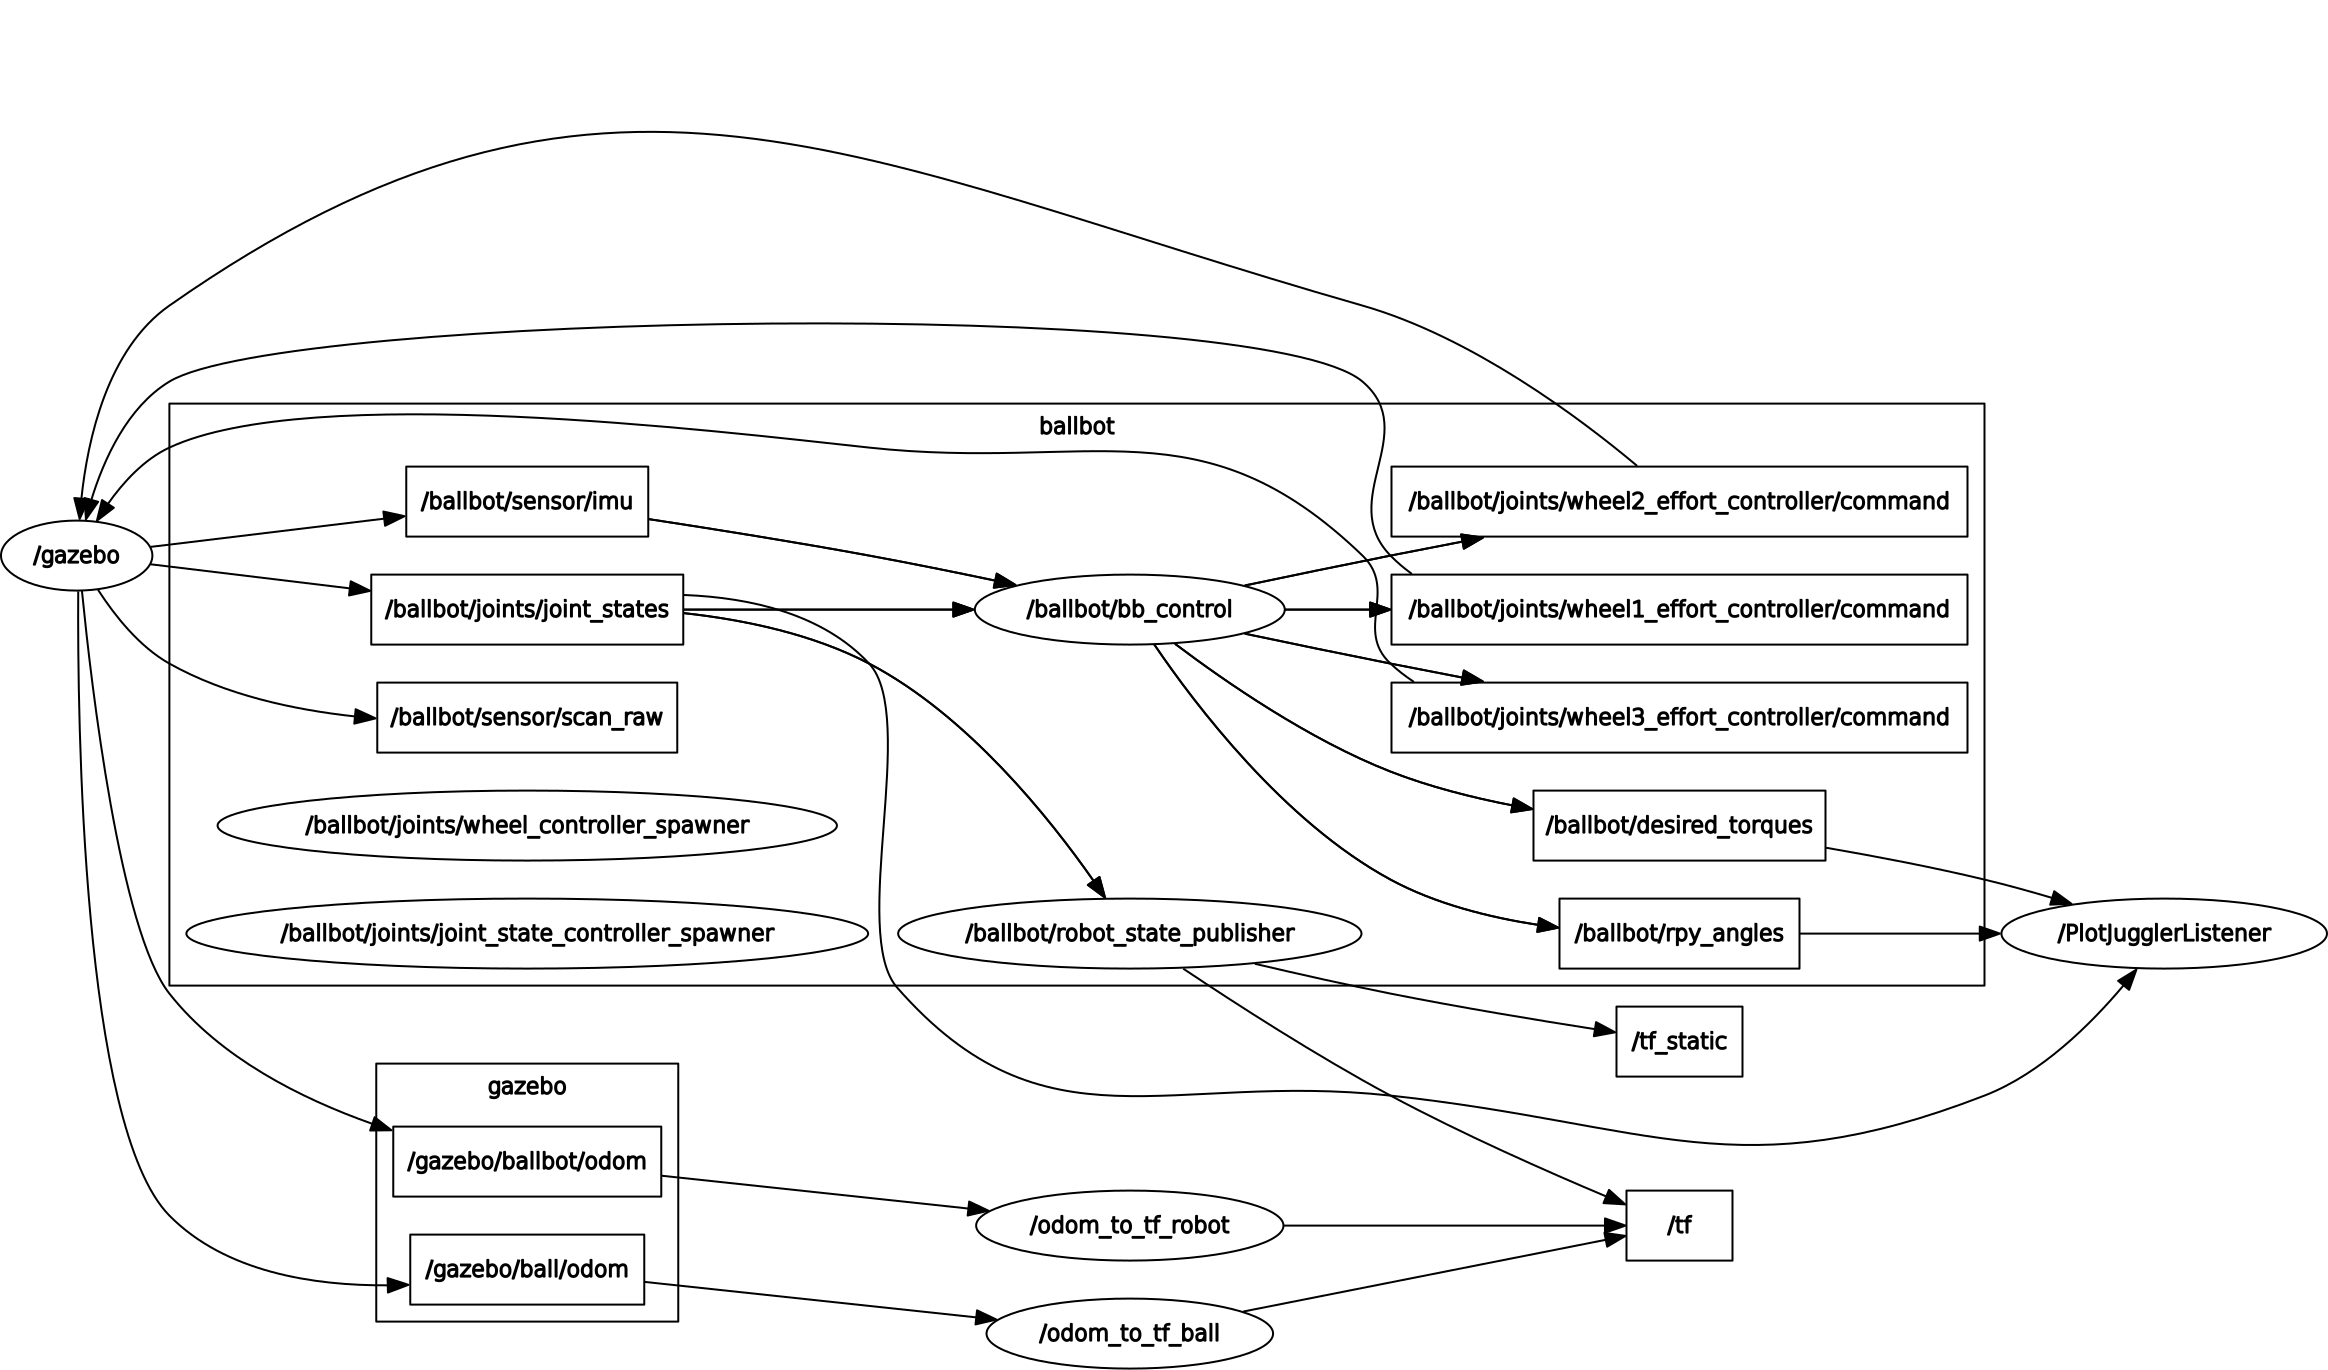
\includegraphics[scale=0.25, angle=90]{./Bilder/Markus/rosgraph.png} }
	\caption{�bersicht aller Teilprogramme(Nodes) und deren Topics, die beim Starten der Simulation aktiv sind und Nachrichten austauschen. Hierbei sind die Nodes mit Ellipsen und die Topics mit Rechtecken gekennzeichnet. Das Bild wurde mit dem ROS Programm rqt\_graph erstellt.}
\end{figure}

\chapter{Simulink Simulationsaufbau} \label{ch:gesamtbild}
\begin{figure}[htbp]%
	{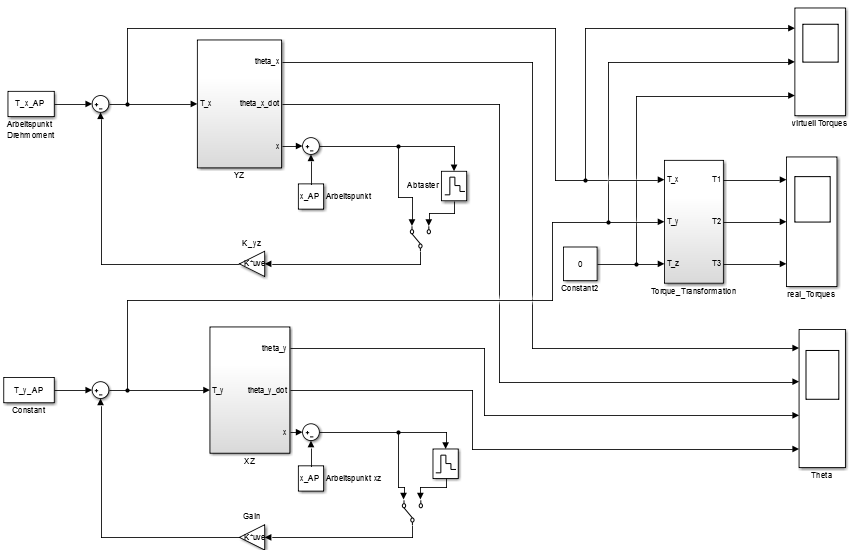
\includegraphics[scale=0.8, angle=90]{./Bilder/Florian/Komplett_System_MATLAB_SIMULINK.PNG} }
	\caption{�bersicht des Simulink Simulationsaufbaus}
\end{figure}




% =================================================================================


%% =================================================================================
%% Abbildungsverzeichnis
%% =================================================================================
%\cleardoublepage
%\phantomsection					% F�r Aufnahme ins Inhaltsverzeichnis
%\addcontentsline{toc}{chapter}{\listfigurename}	% In Inhaltsverzeichnis von
%												% Dokument und pdf aufnehmen
%\listoffigures
%% =================================================================================
%
%% =================================================================================
%% Tabellenverzeichnis
%% =================================================================================
%\cleardoublepage
%\phantomsection					% F�r Aufnahme ins Inhaltsverzeichnis
%\addcontentsline{toc}{chapter}{\listtablename}	% In Inhaltsverzeichnis von
%												% Dokument und pdf aufnehmen
%\listoftables
%% =================================================================================

% =================================================================================
% Literaturverzeichnis
% =================================================================================
\cleardoublepage
\phantomsection					% F�r Aufnahme ins Inhaltsverzeichnis
\addcontentsline{toc}{chapter}{\bibname}	% In Inhaltsverzeichnis von
											% Dokument und pdf aufnehmen
%\bibliographystyle{gerabbrv}	% Verweise nummeriert in eckigen Klammern, alphabetisch sortiert
\bibliographystyle{gerunsrt}	% Verweise nummeriert in eckigen Klammern, nach Erscheinung sortiert


\bibliography{./bib/Literature_flo}	

% Literaturverzeichnis einf�gen, mit Angabe der
								% Bibtex-Datei
% =================================================================================
\end{document}
